\documentclass[11pt, a4paper]{book}
\usepackage[svgnames,table,dvipsnames]{xcolor} % For color names
\usepackage{fontspec} % font selecting commands
\usepackage{tcolorbox} % For colored boxes
\usepackage{graphicx} % For pictures
\usepackage[export]{adjustbox}
\usepackage{polyglossia} % Babel alternative in XeLaTex
\usepackage{fancyhdr} % For page headers
\usepackage[top=2.5cm, bottom=2.5cm, left=3cm, right=2cm]{geometry} % To control page margins
\usepackage{listings} % For source code
\usepackage[colorlinks=true,
            urlcolor=RedOrange,
            unicode=true,
            pdftitle={تعلّم البرمجة بلغة الـC},
            pdfauthor={عدن بلواضح,حمزة عباد,أحمد زبوشي}
            pdfdisplaydoctitle=true]{hyperref} % For hyperlinks and PDF metadata
\usepackage{float}
\usepackage{tabu,booktabs}
\usepackage{bidi}
% Language settings
\setmainlanguage[locale=algeria]{arabic}
\setotherlanguage{english}
\addto\captionsarabic{ % Without this, changes won't take effect, because of Polyglossia
  \renewcommand{\partname}{الجزء}
  \renewcommand{\chaptername}{الفصل}
}
% Font settings
\defaultfontfeatures{Ligatures=TeX}
\newfontfamily\arabicfont[Script=Arabic, Scale=1.2]{Amiri} % An arabic font
\newfontfamily\englishfont[Script=Latin]{Liberation Sans} % Font used for latin text in the document
\newfontfamily\arabicfonttt{Liberation Mono} % Monospace font, for displaying codes
% Boxes definitions
\tcbset{boxrule=0mm, arc=2pt}
\newtcolorbox{question}{colback=blue!70!green!10, colframe=blue!80!green!5, fontupper=\itshape} % Used for question boxes
\newtcolorbox{critical}{colback=red!20, colframe=red!50} % Used for critical warning boxes
\newtcolorbox{warning}{colback=yellow!20, colframe=yellow!50} % Used for warning boxes
\newtcolorbox{information}{colback=blue!5!green!20, colframe=blue!10!green} % Used for information boxes
\newcommand\InlineCode[1]{\fcolorbox{LightGray}{Snow}{\ttfamily \LR{#1}}}
% Titles settings (Make them orange)
\makeatletter
\let\oldchapter\chapter
\newcommand{\@chapterstar}[1]{\cleardoublepage\phantomsection\addcontentsline{toc}{chapter}{#1}{\color{green!30!blue!80}\oldchapter*{#1}}}
\newcommand{\@chapternostar}[1]{{\color{green!30!blue!80}\oldchapter{#1}}}
\renewcommand{\chapter}{\@ifstar{\@chapterstar}{\@chapternostar}}
\let\oldpart\part
\newcommand{\@partstar}[1]{\cleardoublepage\phantomsection\addcontentsline{toc}{part}{#1}{\color{orange}\oldpart*{#1}}}
\newcommand{\@partnostar}[1]{{\color{orange}\oldpart{#1}}}
\renewcommand{\part}{\setcounter{chapter}{0}\@ifstar{\@partstar}{\@partnostar}}
\let\oldsection\section
\newcommand{\@sectionstar}[1]{\phantomsection\addcontentsline{toc}{section}{#1}{\color{orange}\oldsection*{#1}}\sectionmark{#1}}
\newcommand{\@sectionnostar}[1]{{\color{orange}\oldsection{#1}}}
\renewcommand\section{\@ifstar{\@sectionstar}{\@sectionnostar}}
\makeatother
% Pictures settings
\graphicspath{{Pictures/}} % Folder of pictures
\newcommand\Picture[2][]{ % This command automatically centers the picture and fits its size to the page. It supports captions too.
  \begin{center}
    \includegraphics[max size={0.8\textwidth}{0.5\textheight}]{#2}\\
    #1
  \end{center}
}
% Paragraphs settings
\setlength{\parskip}{4mm plus 2mm minus 2mm} % Spacing between paragraphs (+/-)
% Page header and footer settings
\setlength{\headheight}{15pt}
\pagestyle{fancy}
\renewcommand{\chaptermark}[1]{ \markboth{{\chaptername~\thechapter.~#1}}{} }
\renewcommand{\sectionmark}[1]{ \markright{#1} }
\fancyhead{}
\fancyhead[OL]{\rightmark}
\fancyhead[ER]{\leftmark}
\setlength{\footskip}{1.5cm}
% Fixing the issues of the numbering
\renewcommand{\thepart}{\Alph{part}}
\renewcommand{\thechapter}{\Alph{part}.\arabic{chapter}}
\renewcommand{\thesection}{\Alph{part}.\arabic{section}.\arabic{chapter}}
\renewcommand{\thesubsection}{\Alph{part}.\arabic{subsection}.\arabic{section}.\arabic{chapter}}
\renewcommand{\thesubsubsection}{\Alph{part}.\arabic{subsubsection}.\arabic{subsection}.\arabic{section}.\arabic{chapter}}
\setcounter{secnumdepth}{1}
% Global settings for code and console
\lstset{frame=single, basicstyle=\ttfamily, breaklines=true, showlines, aboveskip=\parskip}
% C source code
\lstdefinestyle{C}{language=C, showstringspaces=false, numbers=left,
        keywordstyle=\bfseries\color{RoyalBlue}, commentstyle=\itshape\color{Gray},
        numberstyle=\color{Gray}, stringstyle=\color{Crimson},
        directivestyle=\color{DarkOrange},
        deletekeywords={return,if,else,switch,for,while,do,const,static,sizeof},
    	morekeywords={SDL_Surface,Uint32,SDL_Rect,SDL_Event,SDL_TimerID,SDL_NewTimerCallback,TTF_Font,SDL_Color,
    	FMOD_SYSTEM,FMOD_RESULT,FMOD_SOUND,FMOD_CHANNEL,FMOD_CHANNELGROUP,FMOD_BOOL},
        morekeywords=[2]{return,if,else,switch,for,while,do,const,static,sizeof}, keywordstyle=[2]\bfseries\color{Magenta},
        morekeywords=[3]{printf,scanf,fprintf,fscanf,fputc,fgetc,fputs,fgets,fopen,fclose,fseek,ftell,rewind,srand,rand,
        time,SDL_Delay,SDL_GetTicks,SDL_AddTimer,SDL_RemoveTimer,TTF_OpenFont,TTF_CloseFont,TTF_Init,TTF_GetError,TTF_Quit,
        malloc,free,SDL_CreateRGBSurface,SDL_FreeSurface,SDL_BlitSurface,SDL_LoadBMP,SDL_WM_SetIcon,IMG_Load,SDL_GetError,
        SDL_Init,SDL_Quit,SDL_SetVideoMode,SDL_WM_SetCaption,SDL_FillRect,SDL_Flip,SDL_MapRGB,SDL_SetAlpha,SDL_SetColorKey,
    	SDL_PollEvent,SDL_WaitEvent,SDL_EnableKeyRepeat,SDL_ShowCursor,SDL_WarpMouse,TTF_RenderText_Blended,
    	TTF_SetFontStyle,sprintf,TTF_RenderText_Shaded,FMOD_System_Create,FMOD_System_Init,FMOD_System_Close,
    	FMOD_System_Release,FMOD_System_CreateSound,FMOD_System_PlaySound,FMOD_Sound_Release,FMOD_System_GetChannel,
    	FMOD_System_GetMasterChannelGroup,FMOD_Sound_SetLoopCount,FMOD_Channel_GetPaused,FMOD_Channel_SetPaused,
    	FMOD_Sound_Release,FMOD_ChannelGroup_GetPaused,FMOD_ChannelGroup_SetPaused},
        keywordstyle=[3]\color{RoyalBlue},
}
\lstnewenvironment{Csource}{\lstset{style=C}\setLTR}{\unsetLTR}
% Console
\lstnewenvironment{Console}{\setLTR}{\unsetLTR}
% Table settings
\setlength{\tabulinesep}{2pt}
\setlength{\arrayrulewidth}{2pt}
\taburulecolor{White}
\newenvironment{Table}[1]{ % Accepts 1 parameter which is the number of columns
\taburowcolors[2] 2{LightGray!40 .. LightGray!80}
\begin{center}
  \begin{tabu}{*{#1}{|r}|}
    \toprule
    \rowfont{\bfseries\color{White}}
    \rowcolor{OrangeRed}
    \everyrow{\hline}
}{
  \end{tabu}
\end{center}
}
\newenvironment{Table*}[1]{
\taburowcolors[1] 2{LightGray!40 .. LightGray!80}
\begin{center}
  \begin{tabu}{*{#1}{|r}|}
    \toprule
    \everyrow{\hline}
}{
  \end{tabu}
\end{center}
}

\title{تعلّم البرمجة بلغة الـC}
\begin{document}
  \chapter*{تقديم}
إن التحرّر الفكري في بداية القرن العشرين أدّى إلى توسّع في البحوث العلمية التي شملت كل الميادين لاسيّما التكنولوجية منها كعلوم الحاسوب. هذه الأخيرة أعقبتها ثورة في لغات البرمجة التي تعتبر ركيزة أساسية تقوم عليها البرامج. من بين هذه اللغات نجد لغة الـ\textenglish{C}،
إذ تعتبر من أقوى لغات البرمجة و أكثرها شيوعاً، فهي مستلهمة من طرف لغتي
 \textenglish{B}
 و
 \textenglish{BCPL}
حيث تمّ تطويرها في عام 1972 من طرف
\textenglish{Ken Thompson}
و
 \textenglish{Dennis Ritchie}،
و في ظرف سنة واحدة توسّعت لتكون عِـماد نظام التشغيل
\textenglish{UNIX}
بنسبة
90\%
ثم تم توزيعها في العام المـُوالي رسمياً عبر الجامعات لتصبح بذلك لغة برمجة عالمية. و اشتهرت لغة الـ\textenglish{C}
 كونـُها لغة عالية المستوى، لها مُترجم سريع و فعّال. كما أنها لغة برمجية نقّالة، هذا يعني أن أي برنامج يحترم المعيار
\textenglish{AINSI}
يمكن أن يتمّ تشغيله على أيّة منصّة تحتوي على مترجم
\textenglish{C}
 دون أيّة تخصيصات.

يعتبر هذا الكتاب بوابة سهلة لكلّ مبتدئ لتعلّم لغة الـ\textenglish{C}
خطوة بخطوة بدءً من الأساسيات وصولاً إلى تطوير ألعاب ثنائية الأبعاد و التحكّم في هياكل البيانات الأكثر تعقيداً. الكتاب مرفق بجملة من التمارين و الأعمال التطبيقية المحلولة التي تساعد على هضم المفاهيم المكتسبة و تطبيقها على أيّ مشكل برمجي مهما كان نوعه. و لأن الكثير من لغات البرمجة تعتمد أساساً على الـ\textenglish{C}
كالـ\textenglish{Java}
و الـ\textenglish{C++}\chapter*{تقديم}
إن التحرّر الفكري في بداية القرن العشرين أدّى إلى توسّع في البحوث العلمية التي شملت كل الميادين لا سيّما التكنولوجية منها كعلوم الحاسوب. هذه الأخيرة أعقبتها ثورة في لغات البرمجة التي تعتبر ركيزة أساسية تقوم عليها البرامج. من بين هذه اللغات نجد لغة \textenglish{C}،
إذ تعتبر من أقوى لغات البرمجة وأكثرها شيوعًا، فهي مستلهمة من طرف لغتي
 \textenglish{B}
 و
 \textenglish{BCPL}
حيث تمّ تطويرها في عام 1972 من طرف
\textenglish{Ken Thompson}
و
 \textenglish{Dennis Ritchie}،
و في ظرف سنة واحدة توسّعت لتكون عِـماد نظام التشغيل
\textenglish{UNIX}
بنسبة
90\%
ثم تم توزيعها في العام المـُوالي رسميًا عبر الجامعات لتصبح بذلك لغة برمجة عالمية. واشتهرت لغة \textenglish{C}
 كونـُها لغة عالية المستوى، لها مُترجم سريع و فعّال. كما أنها لغة برمجية نقّالة، هذا يعني أن أي برنامج يحترم المعيار
\textenglish{AINSI}
يمكن أن يتمّ تشغيله على أيّة منصّة تحتوي على مترجم
\textenglish{C}
 دون أيّة تخصيصات.

يعتبر هذا الكتاب بوابة سهلة لكلّ مبتدئ لتعلّم لغة \textenglish{C}
خطوة بخطوة بدءً من الأساسيات وصولًا إلى تطوير ألعاب ثنائية الأبعاد والتحكّم في هياكل البيانات الأكثر تعقيدًا. الكتاب مرفق بجملة من التمارين والأعمال التطبيقية المحلولة التي تساعد على هضم المفاهيم المكتسبة وتطبيقها على أيّ مشكل برمجي مهما كان نوعه. ولأن الكثير من لغات البرمجة تعتمد أساسًا على \textenglish{C}
مثل \textenglish{Java}
و \textenglish{C++}
و \textenglish{C\#}
(لغات برمجية غرضية التوجّه) وحتى
\textenglish{PHP}
(لغة لبرمجة المواقع) فإن تعلّم لغة \textenglish{C}
 سيساعد على تعلّم أيّة لغة برمجية كانت. تبقى الإرادة وحبّ العمل والشغف المفاتيح الرئيسية للنجاح والوصول إلى الاحترافية.

\vfill

\hfill\parbox{0.3\textwidth}{\centering
عدن بلواضح

\vspace{1em}
الجزائر\\[0.5em]
في
24 ذو القعدة 1438\\[0.3em]
الموافق لـ17 أوت 2017
%\Hijritoday\\[0.3em]
%الموافق لـ\today

}


و الـ\textenglish{C\#}
(لغات برمجية غرضية التوجّه) و حتى
\textenglish{PHP}
(لغة لبرمجة المواقع) فإن تعلّم لغة الـ\textenglish{C}
 سيساعد على تعلّم أيّة لغة برمجية كانت. تبقى الإرادة و حبّ العمل و الشغف المفاتيح الرئيسية للنجاح و الوصول إلى الاحترافية.

\vfill

\hfill\parbox{0.3\textwidth}{\centering
عدن بلواضح

\vspace{1em}
الجزائر\\[0.5em]
في
24 ذو القعدة 1438\\[0.3em]
الموافق لـ17 أوت 2017
%\Hijritoday\\[0.3em]
%الموافق لـ\today

}


  \chapter*{مقدّمة}

\vspace{-0.6em}
تحبّ تعلّم البرمجة لكن لا تعرف من أين تبدأ ؟ هذه الدروس لتعليم لغة الـ\textenglish{C}
للمبتدئين قد جُعلت خصّيصاً من أجلك !

\vspace{-0.1em}
لغة الـ\textenglish{C}
هي لغة لا مفرّ منها، أُستلهمَت منها العديد من اللغات الأخرى. تمّ اختراعها في السبعينات و لا تزال مستعملة لحدّ الآن في البرمجة النظامية و عالم الروبوتات. تعتبر لغة الـ\textenglish{C}
لغة معقّدة، لكن إن استطعت تعلّمها ستكوّن لك قاعدة برمجية صلبة !

\vspace{-0.1em}
في هذه الدروس، ستبدأ باكتشاف مبدأ عمل الذاكرة، المتغيرات، الشروط و الحلقات. ثم ستقوم باستعمال كلّ ما تعلّمته في إنشاء واجهات رسومية بالاستعانة بالمكتبة
\textenglish{SDL}
 (ألعاب فيديو، تسجيلات صوتية \dots). أخيراً، ستتعلّم كيف تتعامل مع هياكل البيانات الأكثر شيوعاً من أجل تنظيم المعلومات في الذاكرة : قوائم متسلسلة، مكدّسات، طوابير، جداول تجزئة \dots

\vspace{-0.1em}
التحق بي في هذه الدروس من أجل اكتشاف البرمجة بلغة الـ\textenglish{C} !

\begin{figure}[H]
	\centering
	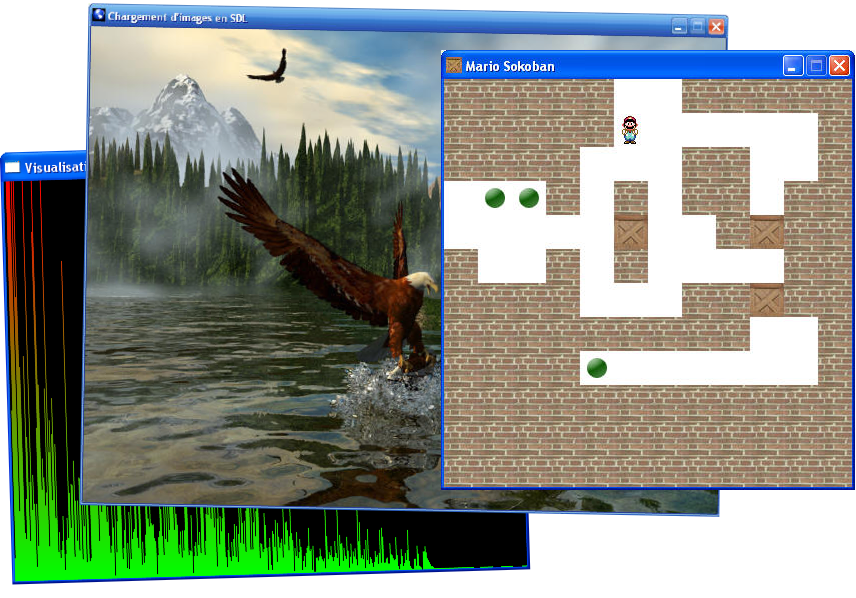
\includegraphics[height=0.4\textheight]{Introduction_original}\\
\small بعض الإنجازات الّتي سنقوم بها في هذا الكتاب
\end{figure}

\vfill
\hfill\parbox{0.3\textwidth}{\centering \textenglish{Mathieu Nebra}\\[0.2em]
مؤسس مشارك لموقع
\href{http://openclassrooms.com/}{\textenglish{OpenClassrooms}}
}

  \part{أساسيّات البرمجة بلغة الـ\textenglish{C}}
  \chapter{قلت برمجة ؟}
\section{ما هي البرمجة؟}
\begin{question}
  ما الذي تعنيه كلمة "بَرْمَجَ"؟
\end{question}

لن أتعبك وأعطيك أصل كلمة "بَرْمَجَ"، لكنني سأختصر كل شيء في جملة: البرمجة تعني إنشاء برامج حاسوب. وهذه البرامج التي تنشئها تأمر الجهاز بالقيام بتعليمات وأفعال معيّنة.
حاسوبك الخاص يحتوي على كثير من هذه البرامج وبمختلف أنواعها:

\begin{itemize}
  \item الآلة الحاسبة تعتبر برنامجاً.
  \item معالج النصوص يعتبر برنامجاً أيضاً.
  \item وكذلك برنامج المحادثة.
  \item ألعاب الفيديو هي برامج كذلك.
\end{itemize}

\Picture[\caption{نسخة عن لعبة \textenglish{MetalSlug} الشهيرة تم إنشاؤها من طرف العضو \href{http://www.siteduzero.com/membres-294-176405.html}{\textenglish{joe87}}}]{Chapter_I-1_MetalSlug}
باختصار البرامج موجودة في كل جهاز، وهي التي تعطي الحاسوب قدرته على إنجاز مختلف المهام التي تُخوَّل إليه. يمكنك أن تنشئ برنامج تشفير أو لعبة ثنائية / ثلاثية الأبعاد باستخدام لغة برمجة مثل \textenglish{C}.

ملاحظة: لم أقل أن إنشاء لعبة يتم برمشة عين، لقد قلت فقط بأنه شيء ممكن، لكن كن متأكداً، سوف يتطلب ذلك جهدا كبيراً!

وبما أننا في بداية الطريق، فإّننا لن نقوم بإنشاء لعبة ثلاثية الأبعاد! لكنّنا سنبدأ بكيفية عرض نص على الشاشة، طبعا ستقول ما علاقة هذا بإنشاء الألعاب؟ لكن ثِق بي، هذا الأمر ليس بسيطا كما يبدو!

بالطبع هذا ليس شيئا مُبهراَ، ولكن يجب علينا أن نبدأ من هنا؛ وشيئا فشيئا يمكنك أن تنشئ برامج معقّدة أكثر. فالهدف من هذا الدرس هو أن أعرفك على كل ما يتعلق بهذه اللغة.

\section{البرمجة، بأي لغة يا ترى؟}
حاسوبك هو آلة غريبة جداً، هذا أقل ما يمكن أن نقوله عنه. يمكننا أن نخاطبه فقط بالصفر والواحد، فمثلا إذا طلبنا منه حساب 3+5 فيمكن لهذا أن يعطينا نتيجة كالتالي (هذه ليست ترجمة دقيقة ولكنها تشبه ما يحدث بالفعل):\\
\InlineCode{0010110110010011010011110}

ما تَرَاه هنا يسمى اللغة الثنائية
(\textenglish{Binary language})
أو لغة الآلة
(\textenglish{Machine language})،
وحاسوبك لا يفهم سوى هذه اللغة، وكما تلاحظ، هذه اللغة غير مفهومة على الإطلاق!

مشكلتنا الآن:
\begin{question}
  كيف يمكننا التعامل مع حاسوب لا يفهم سوى اللغة الثنائية؟
\end{question}

حاسوبك لا يتحدث الإنجليزية، ولا العربية، ولا أي لغة غير هذه اللغة، ولكنها صعبة جدا لدرجة أن حتى أكبر خبراء الحاسوب لا يستخدمونها.
لهذا قام بعض مهندسي الحواسيب باختراع لغات يمكن أن تُتَرجَمَ إلى اللغة الثنائية، لكن الشيء الأصعب هو إنشاء البرامج الّتي تقوم بهذه الترجمة. ولحسن الحظ فقد قاموا بهذا العمل نيابة عنا. هذه البرامج تقوم بترجمة الأوامر الّتي تكتبها (مثلا: "أُحسب 3+5") إلى شيء يشبه هذا:
\InlineCode{0010110110010011010011110}.

هذا المخطط يلخص ما كنت أشرح:

\Picture{Chapter_I-1_Translation}

\section{قليل من المفردات}
حتّى الآن كنت أتحدّث إليك بكلمات بسيطة، لكن يجب أن تعلم أنه في المعلوماتية توجد مصطلحات علمية لكل ما ذكرت. طوال هذا الدرس، سوف تتعلم استخدام المفردات المناسبة. هذا سيفيدك كثيرا خصوصا عندما تتحدث مع مبرمجين آخرين، حيث أنك سوف تتفاهم معهم بكل سهولة.

نعود إلى الحديث عن المخطط السابق في المستطيل الأول قلت أن "برنامجك مكتوب بلغة مُبَسَّطة"، في الواقع هذا النوع من اللغات يُعرف باسم لغات البرمجة عالية المستوى (\textenglish{High-level programming languages}). هناك مستويات عديدة من لغات البرمجة، وكلما كان مستوى اللغة أعلى كانت أقرب إلى اللغة الحقيقية وكان استخدامها أسهل. إذن، اللغات عالية المستوى سهلة الاستخدام لكنها تتضمن بعض السلبيّات سوف نتعرّف عليها لاحقا.

توجد العديد من لغات البرمجة، وهي متفاوتة المستوى، منها:
\begin{itemize}
  \item \textenglish{C}
  \item \textenglish{C++}
  \item \textenglish{Java}
  \item \textenglish{Visual Basic}
  \item \textenglish{Delphi}
  \item و العديد غيرها
\end{itemize}

كما تلاحظ، لم أرتبها حسب مستوياتها، لذلك لا تعتقد أن اللغة الأولى في القائمة هي الأسهل أو العكس. عموما، لائحة اللغات الموجودة طويلة جدا لدرجة أنه لا يمكنني كتابتها كلها هنا.

مصطلح آخر يجب تذكّره هو
\underline{الشفرة المصدرية}
(\textenglish{Source code})،
 وهي ببساطة الشفرة الخاصة ببرنامجك الذي تكتبه بلغة عالية المستوى والذي يتم ترجمته فيما بعد إلى اللغة الثنائية.

 ثم يأتي دور البرنامج الذي يحوّل هذه اللغة عالية المستوى إلى اللغة الثنائية، هذا النوع من البرامج يعرف باسم
 \underline{المترجم}
  أو
  \underline{المصنّف}،
 والعملية الّتي يقوم بها تسمى
 \underline{الترجمة}
 أو
 \underline{التصنيف}.

\begin{information}
  يوجد لكل لغة عالية المستوى مترجم خاص، وهذا شيء منطقي، فاللغات مختلفة فيما بينها، فلا يمكننا ترجمة لغة
\textenglish{C}
بنفس الطريقة الّتي نترجم بها
\textenglish{Delphi}
مثلا.
  بعض اللغات مثل
\textenglish{C}
تملك العديد من المترجمات، فمنها من هو مكتوب من طرف
\textenglish{Microsoft}
، و منها من
\textenglish{GNU}
، إلخ… سوف نتعرّف على كل هذا في الدرس القادم.
  لحسن الحظ، هذه المترجمات متطابقة تقريبا (رغم وجود اختلافات طفيفة بينها سوف نتعرف عليها لاحقا).
\end{information}

أخيرا، البرنامج الثنائي المنشئ بواسطة المترجم يسمى الملف
\underline{القابل للتنفيذ}
أو
\underline{التنفيذي}
(\textenglish{Executable}).
 لهذا السبب تملك البرامج
 (على الأقل برامج
 \textenglish{Windows})
 الامتداد
\textenglish{.exe}
 والذي هو اختصار كلمة
 \textenglish{EXEcutable}.

 نعود إلى مخططنا السابق، وهذه المرة سنستخدم المصطلحات الصحيحة:

 \Picture{Chapter_I-1_Compilation}

 \section{لماذا نختار تعلّم \textenglish{C}؟}
 كما قلت سابقا، يوجد كثير من اللغات عالية المستوى، فلماذا ينبغي علينا أن نبدأ بإحداها على وجه الخصوص؟ سؤال عظيم!

على أية حال يجب علينا أن نختار بأي لغة سنبدأ البرمجة عاجلا أم آجلا، وبالتالي لديك الخيار في البدء بـ:
\begin{itemize}
  \item \textbf{لغة ذات مستوى عالي جدّا}:
 وتكون سهلة جدّا أوعامة، نذكر من بينها
 \textenglish{Python}، \textenglish{Ruby}، \textenglish{Visual Basic}،
 وغيرها. هذه اللغات تسمح بكتابة برامج بشكل أسرع. عامّة تحتاج لأن تُرفق معها ملفات مُسَاعِدة لكي تعمل (كَمُفَسِّرٍ مثلا).
  \item \textbf{لغة ذات مستوى منخفض قليلا}:
هي أكثر صعوبة نوعا ما، ولكن مع لغة مثل
\textenglish{C}
 سوف تتعلم كثيرا عن البرمجة وحول طريقة عمل حاسوبك. ستكون بعد ذلك قادراً على تعلّم لغة برمجة أخرى إن أردت وبكل يُسْرٍ.
\end{itemize}

من ناحية أخرى،
\textenglish{C}
لغة برمجة واسعة الإنتشار، أُستخدمت في برمجة العديد من البرامج التي تعرفها. حتى أنها كثيرا ما تدرّس في الدراسات العليا في مجال المعلوماتية.
هذه هي الأسباب الّتي جعلتني أتحمّس لتعليمك لغة
\textenglish{C}
بالتحديد. لم أقل أنّه يجب عليك أن تبدأ بها، لكنّي قلت إنه خيار جيّد لكي أقدّم لك معرفة صلبة في هذا الدرس.

\begin{information}
  بعض لغات البرمجة موجّهة أكثر للشبكة العنكبوتية
 (\textenglish{Web})
 مثل
 \textenglish{PHP}
 أكثر منها من إنشاء البرامج المعلوماتية.
\end{information}

سوف أفترض في هذا الكتاب أنّ هذه هي لغة برمجتك الأولى وأنّه لم يسبق لكم أن برمجت من قبل. فإن كنت قد برمجت قليلا من قبل فلا مضرّة في أن تعيد من الصفر.

\begin{question}
  ما هو الفرق بين
  \textenglish{C}
  و
  \textenglish{C++}
  ؟
\end{question}

هاتان اللغتان قريبتان جدّا من بعضهما، وكلاهما مستخدمتان بكثرة. ولكي تعرف كيف نشأتا يجب عليك أن تدرس التاريخ قليلا:
\begin{itemize}
  \item في البداية، عندما كانت الحواسيب تَزِنُ أطنانا وتشغل مكانا قَدْرُهُ حجم منزلك، تمّ إختراع لغة برمجة تسمّى
\textenglish{Algol}.
  \item بعدها تطوّرت الأمور أكثر واختُرعَت لغة برمجة جديدة عُرِفَتْ باسْمِ
\textenglish{CPL}
 والّتي تطوّرت فيما بعد إلى لغة
\textenglish{BCPL}
 ثم أخذت إسم اللغة
\textenglish{B}.
  \item مع مضيّ الزمن توصّل الخبراء إلى ابتكار اللغة
\textenglish{C}
 وقد تمّ إدخال بعض التعديلات عليها إلّا أنها لا تزال من أحد اللغات الأكثر استخداما اليوم.
  \item وبعد زمن، أراد الخبراء أن يضيفوا بعض الأشياء إلى
\textenglish{C}
، يمكن اعتبارها نوعا من التحسينات. والنتيجة كانت بما يعرف بلغة
\textenglish{C++}
، وهي لغة
\textenglish{C}
 مع إضافات تمكّننا من البرمجة بطريقة مختلفة.
\end{itemize}

\begin{information}
  الـ
\textenglish{C++}
ليست أحسن من الـ
\textenglish{C}
، هي فقط تمكننا من البرمجة بطريقة مختلفة وتساعد المبرمج على تنظيم شفرة برنامجه. رغم ذلك هي تشبه الـ
\textenglish{C}
كثيرا. وإن كنت تنوي تعلّم الـ
\textenglish{C++}
فيما بعد فَسَوْفَ تجد ذلك سهلا.
\end{information}

ولو اعتُبرت
\textenglish{C++}
 تطويرا لـ
\textenglish{C}
 فإن هذا لا يعني أنه يجب استخدام
\textenglish{C++}
 فقط لإنشاء البرامج. لغة
\textenglish{C}
 ليست لغة عجوزا منسيّة، بالعكس هي مستخدمة بكثرة اليوم. بل إنها أساس أنظمة التشغيل الكبيرة مثل
\textenglish{Unix }
(ومنه
\textenglish{GNU/Linux}
 و
\textenglish{Mac OS}) و
\textenglish{Windows}.

\section{هل البرمجة صعبة؟}
هذا سؤال يعذّب روح كل من يريد تعلّم البرمجة! هل يجب أن تكون أستاذ رياضيات كبير درس 10 سنوات من التعليم العالي حتّى تبدأ البرمجة؟

الجواب هو لا بالطبع. كل ما تحتاج إليه هو معرفة العمليات الأربع الأساسية:
\begin{itemize}
  \item الجمع
  \item الطرح
  \item الضرب
  \item القسمة
\end{itemize}
هذا ليس مخيفا! سوف أشرح لك في درس لاحق كيف يقوم الحاسوب بهذه العمليات الأساسية في برامجك.

باختصار، لا توجد صعوبات غير قابلة للحلّ. في الواقع، هذا يعتمد على طبيعة برنامجك، فإذا كنت تريد إنشاء برنامج تشفير فيجب عليك معرفة بعض الأشياء في الرياضيات، وإن كان برنامجك يقوم بالرسم ثلاثي الأبعاد فيجب أن تكون لديك بعض المعرفة بالهندسة الفضائية.

كل حالة تعامل بطريقة خاصّة. ولكن لتعلّم لغة
\textenglish{C}
 نفسها لا تحتاج إلى أيّة معارف قبليّة.

\begin{question}
  إذن أين هو الفخ؟ وأين تكمن الصعوبة؟
\end{question}

يجب أن تعرف كيف يعمل الحاسوب، لتفهم ما الّذي نقوم به في C. من هذا المنطلق، كن متيقّنا أنّي سأعلّمك كلّ هذا شيئا فشيئا.

اعلم أن للمبرمج صفات أيضا مثل:
\begin{itemize}
  \item الصبر: البرنامج لا يعمل عادة من أوّل محاولة، يجب أن تكون مثابراً.
  \item حسّ المنطق: صحيح أنّك لست بحاجة إلى أن يكون لديك مستوى جيّد في الرياضيّات، لكنّ هذا لا يمنع من التفكير وتحليل المشكلات بالمنطق.
  \item الهدوء: فيجب عليك ألّا تضرب حاسوبك بالمطرقة، فهذا لن يجعل برنامجك يعمل!
\end{itemize}

  \chapter{الحصول على الأدوات اللازمة}

بعد تجاوزنا لفصل تمهيدي مليئ بالثرثرة سوف نبدأ بالدخول في صلب الموضوع. سوف نجيب عن السؤال التالي : "ما هي البرامج التي نحتاج إليها للبدء في البرمجة ؟".

لا يوجد شيء صعب في هذا الفصل، سوف نأخذ وقتنا للتأقلم على هذه البرامج الجديدة.

اغتنم الفرصة ! في الفصل التالي سنبدأ حقّا في البرمجة و لن يكون هناك وقت للقيلولة !

\section{الأدوات اللازمة للمبرمج}

إذن ما هي الأدوات التي نحتاج إليها ؟
إذا تابعت الفصل السابق جيّدا، فستعرف واحدا على الأقل !

هل تعلم عمّا أتحدّث ؟ حقّا لا ؟

حسنا، نحن نتحدّث عن
\textbf{المترجم}
الذي يمكّن من ترجمة لغة الـ\textenglish{C}
إلى اللغة الثنائيّة !

كما قلت لك في الفصل الأوّل، يوجد العديد من المترجمات للغة الـ\textenglish{C}.
سنرى أن اختيار المترجم ليس أمرا معقّدا في حالتنا هذه.

ما الذي نحتاج إليه أيضا ؟ لن أتركك تخمّن كثيرا و سأعطيك القائمة :

\begin{itemize}
  \item \textbf{محرّر نصوص }
(\textenglish{Text Editor})
لكتابة الشفرة المصدرية الخاصّة بالبرنامح. نظريّا برنامج تحرير نصوص بسيط مثل
\textenglish{Notepad}
على
\textenglish{Windows}
أو
\textenglish{vi}
على
\textenglish{Unix}
يكفي، لكن من الأحسن استخدام محرّر نصوص ذكيّ يقوم بتلوين الشفرة المصدرية لكي يسهّل عليك العمل.
  \item \textbf{مترجم}
  لتحويل الشفرة المصدرية إلى ملف ثنائي.
  \item \textbf{المنقّح}
(\textenglish{Debugger})
لمساعدك على كشف الأخطاء في برنامجك. لسوء الحظ، لم نتمكّن بعد من ابتكار "المصحّح" الّذي يصحّح أخطائك لوحده. لكن، إن أحسنت استخدام المنقّح، يمكنك ببساطة إيجاد الأخطاء.
\end{itemize}

وجود مكتشف الأخطاء لا يعنى أن تتصرف بتهوّر و تسرع في كتابة برنامج مليء بالأخطاء، بل تريّث و كن هادئاً.

من الآن لدينا خياران :

\begin{itemize}
  \item إمّا أن نحصل على البرامج الثلاثة متفرّقة و هذه هي الطريقة الأكثر تعقيدا، و لكنّها تعمل. على
\textenglish{GNU/Linux}
تحديدا، عدد كبير من المبرمجين يفضّلون استخدام كلّ برنامج على حدة. لن أشرح هذه الطريقة هنا، بل سأتحدّث عن الطريقة الأسهل.
  \item أو أن تحصل على برنامج "ثلاثة في واحد" يتضمّن محرّر النصوص و المترجم و المنقّح. هذا النوع من البرامج يعرف باسم "بيئات التطوير المتكاملة"
(\textenglish{Integrated Development Environments})
و تسمّى اختصارا
\textenglish{IDE}.
\end{itemize}

يوجد العديد من بيئات التطوير. بداية، قد تواجه صعوبة في اختيار البيئة الملائمة لك. الشيء الأكيد هو : أي بيئة مهما كانت ستحقق لك العمل المطلوب.

\subsection{اختيار البيئة الخاصة بك}

بدا لي أنه من الأفضل أن أريك بعضا من البيئات الشهيرة و المجانيّة في نفس الوقت. شخصيّا، أنا أستخدمها جميعا و أختار في كل يوم  واحدا منها.

\begin{itemize}
  \item أحد هذه البيئات الّتي أفضّلها هو
\textbf{\textenglish{Code::Blocks}}.
هو مجّاني و يعمل على أغلب أنظمة التشغيل. أنصح كلّ مبتدئ أن يختاره للبدء (و في ما بعد أيضا إذا شعرت أنّه يلائمك جيّدا !).

يعمل على أنظمة التشغيل
\textenglish{Windows}،
\textenglish{Mac OS}
و
\textenglish{GNU/Linux}.
  \item الأكثر شهرة على
\textenglish{Windows}
هو الّذي أنشأته
\textenglish{Microsoft}،
إنّه
\textbf{\textenglish{Visual C++}}.
هو برنامج مدفوع (و باهظ الثمن) لكن لحسن الحظّ توجد نسخة مجانية منه تسمّى
\textbf{\textenglish{Visual Studio Express}}
(أنا أستخدم النسخة القديمة
\textbf{\textenglish{Visual C++ Express}}
في هذا الكتاب). و هي ممتازة جدّا (بينها و بين النسخة المدفوعة فوارق طفيفة). إنه برنامج كامل و يملك منقّحا قويّا.

يعمل على
\textenglish{Windows}
فقط.
  \item على
\textenglish{Mac OS X}
يمكنك استخدام
\textbf{\textenglish{Xcode}}
الّذي يفترض أن يكون متوفّرا على قرص تثبيت النظام. يناسب كثيرا مبرمجي
\textenglish{Mac}.

يعمل على
\textenglish{Mac OS X}
فقط.
\end{itemize}

\begin{information}
  ملاحظة لمستخدمي
  \textenglish{GNU/Linux} :
  يوجد العديد من البيئات لهذا النظام، و لكن المبرمجين المحترفين قد يفضّلون تجاوز البيئات و القيام بالترجمة "يدويّا"، و هو شيء أصعب قليلا. نحن سنبدأ باستخدام بيئات تطويرية. لذلك أنصحك بثبيت
  \textenglish{Code::Blocks}
  إن كنت على
  \textenglish{GNU/Linux}
  لكي تتمكن من متابعة شروحاتي.
\end{information}

\begin{question}
من هي البيئة الأفضل من بين كلّ بيئات التطوير هذه؟
\end{question}

كل واحدة من هذه البيئات تمكنك من البرمجة و متابعة بقيّة الكتاب من دون أيّة مشاكل. بعضها كامل أكثر من ناحية المميزات، و أخرى سهلة الإستخدام أكثر، ولكن في كلّ الأحوال البرامج الّتي تنشؤها تكون ذاتها أيّا كانت البيئة التي اِخْتَرْتها. فهذا الخيار ليس بالأهمّية الّتي تعتقدها.

في هذا الكتاب سوف أستخدم
\textenglish{Code::Blocks}.
فإن أردت الحصول على نفس لقطات الشاشة خاصّتي، خصوصا لكي لا تضيع في البداية، أنصحك بِدَايَةً بتثبيت
\textenglish{Code::Blocks}.

\section{\textenglish{Code::Blocks} (\textenglish{Windows, Mac OS X, GNU/Linux})}

\textenglish{Code::Blocks}
هي بيئة تطوير متكاملة حرّة و مجانيّة، متوفّرة للـ\textenglish{Windows}،
\textenglish{Mac}
و
\textenglish{GNU/Linux}.

حاليّا
\textenglish{Code::Blocks}
متوفّر بالإنجليزيّة فقط. لكن هذا ليس أمرا يدعوك إلى تجنّب استخدامه ! فنحن قلّما نحتاج إلى العمل بقوائم واجهته، فلغة
\textenglish{C}
هي الّتي تهمّنا.

كن على علم أنه عندما تبرمج سوف تقابل عادة توثيقا بالإنجليزية. هذا سبب آخر يدفعك للتدرّب على استخدام هذه اللغة.

\subsection{تنزيل \textenglish{Code::Blocks}}

توجّه إلى صفحة تنزيل
\textenglish{Code::Blocks}

\url{http://www.codeblocks.org/downloads/binaries}

ثمّ نزّل الملف الذي يناسب نظامك :

\begin{itemize}
  \item إذا كنت تستخدم
\textenglish{Windows}،
اذهب إلى القسم
"\textenglish{Windows}"
في أسفل الصفحة. نزّل البرنامج الّذي يحوي
\InlineCode{mingw}
في اسمه (مثلا :
\InlineCode{codeblocks-10.05mingw-setup.exe}).
النسخة الأخرى لا تحوي مترجما، لن تتمكن في حال استخدمتها من ترجمة برامجك !
  \item إذا كنت تستخدم
\textenglish{GNU/Linux}،
اختر الحزمة الّتي تناسب توزيعتك.

  \item إذا كنت تستخدم
\textenglish{Mac}،
اختر الملف الأحدث في القائمة، مثلا :
\InlineCode{codeblocks-10.05-p2-mac.zip}.

\end{itemize}

\begin{critical}
أقول و أكرّر : إذا كنت تستخدم
\textenglish{Windows}
فيجب عليك تنزيل النسخة الّتي يتضمَن اسمها كلمة
\textenglish{mingw}
لأنّه إذا اخترت النسخة الخاطئة فلن تتمكّن من ترجمة برامجك فيما بعد !
\end{critical}

التثبيت بسيط و سريع.  أترك جميع الخيارات كما هي و شغّل البرنامج. سوف تظهر لك نافذة شبيهة بهذه :

\begin{figure}[H]
	\centering
	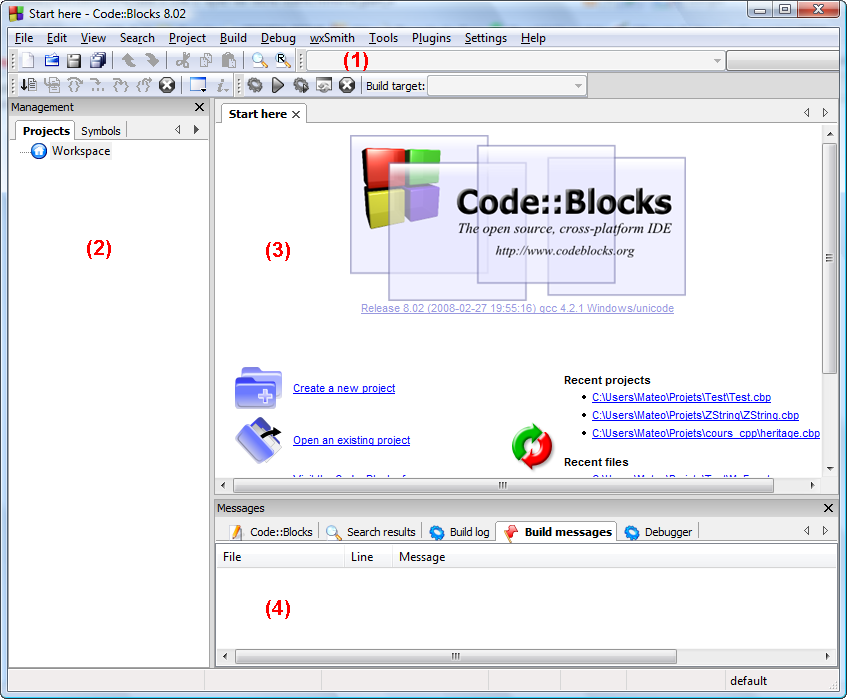
\includegraphics[width=\textwidth]{Chapter_I-2_CodeBlocks}
\end{figure}

نميّز أربعة أقسام رئيسية في واجهة البرنامج، و هي مرقّمة في الصورة :

\begin{enumerate}
  \item شريط الأدوات
(\textenglish{Toolbar}) :
يحتوي على كثير من الأزرار و لكنّنا سوف نستخدم بعضها فقط باستمرار، سأعود للحديث عن هذا فيما بعد.
  \item قائمة ملفات المشروع : توجد بيسار النافذة، تحتوي على كلّ الملفات المصدريّة المتعلقة بالبرنامج الذي تعمل عليه. تكون فارغة في البداية لأننا لم ننشئ أي ملف لحد الآن. سوف نبدأ بملأها خلال خمس دقائق من الآن بتقدّمك في هذا الفصل.
  \item المنطقة الرئيسية : هنا المساحة التي تكتب فيها الشفرة المصدرية الخاصة ببرنامجك بلغة الـ\textenglish{C}.
  \item منطقة الإشعار : و يدعوها البعض "منطقة الموت"، هنا تُعْرَضُ أخطاء الترجمة إذا كانت شفرة البرنامج تحوي خطأً ما. هذا الشيء يحدث كثيرا !
\end{enumerate}

ما يهمّنا الآن هو قسم محدد من شريط الأدوات. تجد فيه الأزرار التالية (بهذا الترتيب) :
\InlineCode{Compile}،
\InlineCode{Execute}،
\InlineCode{Compile \& Execute}،
\InlineCode{Recompile everything}
تذكّرهم جيّدا لأننا سنستخدمهم بانتظام.

\begin{figure}[H]
	\centering
	
\includegraphics{Chapter_I-2_Compile-toolbar}
\end{figure}

و هذا شرح عمل كلّ واحد من هذه الأزرار :

\begin{itemize}
  \item \textbf{\textenglish{Compile}} :
كل ملفّات الشفرة المصدرية الّتي كتبتها يتم ارسالها إلى المترجم الّذي يقوم بإنشاء الملف التنفيذي في حالة عدم وجود أخطاء. أمّا في حالة العثور على أخطاء (و هذا سيحدث عاجلا أم آجلا~!) فلن يتمّ إنشاؤه بل يعرض رسائل خطأ في منطقة الإشعار.
  \item \textbf{\textenglish{Execute}} :
يقوم بتشغيل آخر ملف تنفيذي تمّت ترجمته. يعني أنك ستستخدم هذا الزر لاختبار برامجك الّتي أنشأتها. طبعا يجب عليك ترجمة البرنامج قبل تشغيله. يمكننا أيضا استخدام الزرّ الثالث.
  \item \textbf{\textenglish{Compile \& Execute}} :
لا يجب أن تكون عبقريا لكي تعرف أنّه ليس إلا مجموع الزرّين السابقين. في الواقع هذا هو الزرّ الّذي ستستخدمه أكثر. في حالة ما إذا حدثت أخطاء في الترجمة لن يتمّ تشغيل البرنامج بل ستُعرض قائمة جميلة من الأخطاء التي يجب عليك تصحيحها أوّلا !
  \item \textbf{\textenglish{Recompile everything}} :
 عندما نستخدم
\textbf{\textenglish{Compile}}
يقوم
\textenglish{Code::Blocks}
في الحقيقة بترجمة الملفات الّتي عدّلتها فقط. أحيانا -فقط أحيانا- قد تحتاج إلى إعادة ترجمة جميع الملفّات. سنتحدّث لاحقا عن فائدة هذا الزر و أيضا عن كيفية عمل الترجمة بمزيد من التفصيل. حاليا لكي لا تختلط الأمور عليك يمكنك أن تعتبر أنّه غير مهمّ.
\end{itemize}

\begin{information}
أنصحك باستخدام اختصارات لوحة المفاتيح بدلا من الضغط على الأزرار، لأنّه شيء نكرّره كثيرا. تذكّر خصوصا أنّه يمكنك الضغط على
\InlineCode{F9}
بدل الزر
\InlineCode{Compile \& Execute}.
\end{information}

\subsection{إنشاء مشروع جديد}

لإنشاء مشروع جديد إذهب إلى قائمة
\InlineCode{File}
ثمّ
\InlineCode{New}
ثمّ
\InlineCode{Project}.
من النافذة الّتي تظهر اختر
\InlineCode{Console application}.

\begin{figure}[H]
	\centering
	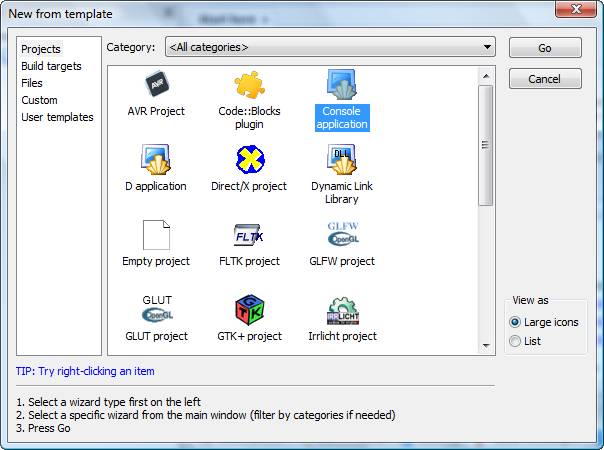
\includegraphics[width=0.8\textwidth]{Chapter_I-2_CodeBlocks-New-project}
\end{figure}

\begin{information}
كما تَرَى،
\textenglish{Code::Blocks}
يقترح عليك إنشاء عدد معتبر من أنواع البرامج الّتي تستخدم مكتبات
(\textenglish{Libraries})
معروفة مثل
\textenglish{SDL}
للـ\textenglish{2D}
و
\textenglish{OpenGL}
للـ\textenglish{3D}
و
\textenglish{Qt}
و
\textenglish{wxWidgets}
لإنشاء النوافذ الرسوميّة. حاليّا، هذه الأيقونات ليست سوى للزينة لأنّ المكتبات السابقة غير مثبّتة على حاسوبك لهذا لا يمكنك أن تجعلها تعمل. سوف نعود لهذه الأنواع الأخرى لاحقا. في هذه الأثناء لا يمكننا سوى أن نستخدم الـ\textenglish{Console}
لأنّك لا تملك بعد المستوى اللازم لانشاء أنواع أخرى من البرامج.
\end{information}

أنقر على
\InlineCode{Go}
لانشاء المشروع الجديد. ثم أنقر على
\InlineCode{Next}
فالصفحة الأولى ليس مهمّة. بعدها سيأتيك اختيار بين لغتي الـ\textenglish{C}
أو الـ\textenglish{C++}،
اختر الـ\textenglish{C}.

\begin{figure}[H]
	\centering
	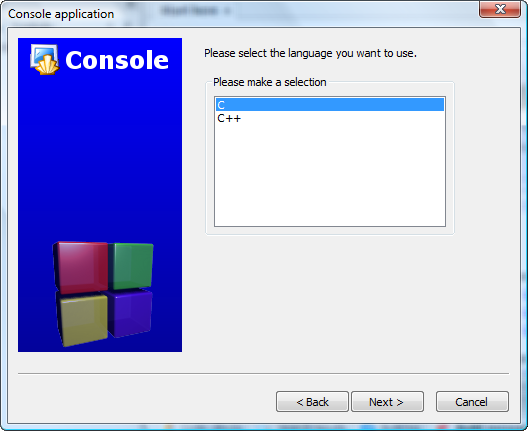
\includegraphics[width=0.8\textwidth]{Chapter_I-2_CodeBlocks-C}
\end{figure}

سيُطْلَبُ منك الآن إدخال اسم المشروع، و كذلك مسار المجلّد الذي تختاره لحفظ الملفّات فيه.

\begin{figure}[H]
	\centering
	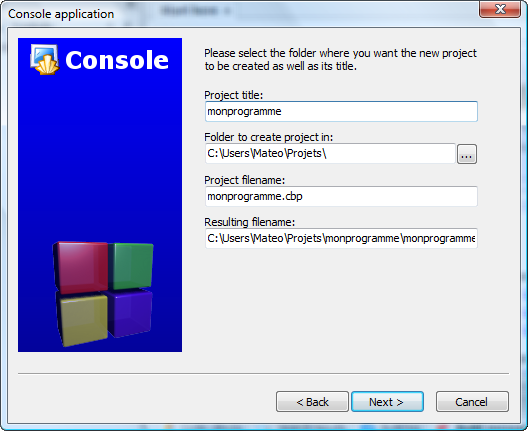
\includegraphics[width=0.8\textwidth]{Chapter_I-2_CodeBlocks_project-path}
\end{figure}

آخر خطوة تُطلب منك هي ، كيف ينبغي أن يترجم البرنامج، يمكنك ترك الخيارات على حالها، لن يكون لهذا أي تأثير على ما سنقوم به الآن (تأكّد أن إحدى الخانتين
"\textenglish{Release}"
أو
"\textenglish{Debug}"
تكون محدّدة على الأقل).

\begin{figure}[H]
	\centering
	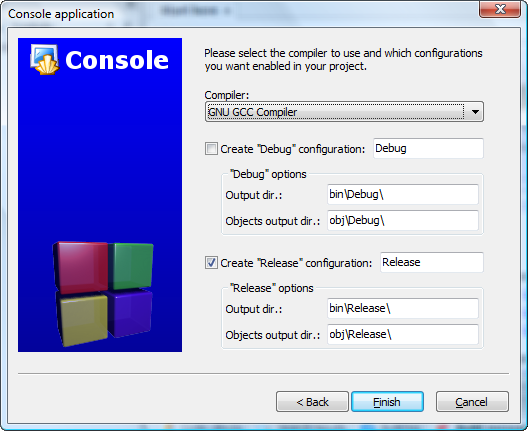
\includegraphics[width=0.8\textwidth]{Chapter_I-2_CodeBlocks_Compiler}
\end{figure}

إضغط على
\InlineCode{Finish}،
إنتهى !\\
لقد قام
\textenglish{Code::Blocks}
بإنشاء المشروع الأوّل و ملئه ببعض الشفرة المصدرية.

في الخانة الخاصة بالمشاريع على اليسار، قم بتوسيعها بالضغط على
'\InlineCode{+}'
لكي تظهر قائمة الملفات في المشروع. سيكون لديك على الأقل ملف يسمّى
\InlineCode{main.c}.
هذا هو كلّ شيء !

\section{\textenglish{Visual C++} (\textenglish{Windows} فقط)}

بعض التذكيرات حول
\textenglish{Visual C++} :

\begin{itemize}
  \item إنها البيئة التطويرية الخاصة بـ\textenglish{Microsoft}.
  \item برنامج مدفوع في الأصل، لكن توجد نسخة مجّانية منه تسمّى \textenglish{Visual C++ Express}.
  \item تمكّن من البرمجة باستخدام كلتا اللغتين
\textenglish{C}
و
\textenglish{C++}
(و ليس فقط
\textenglish{C++}
كما يوحي الاسم).
\end{itemize}

طبعا ستقوم بتحميل النسخة المجانية
\textenglish{Visual C++ Express}
(احذر، هو غير متوافق مع
\textenglish{Windows 7}
إلّا بداية من النسخة 2010) :

\begin{figure}[H]
	\centering
	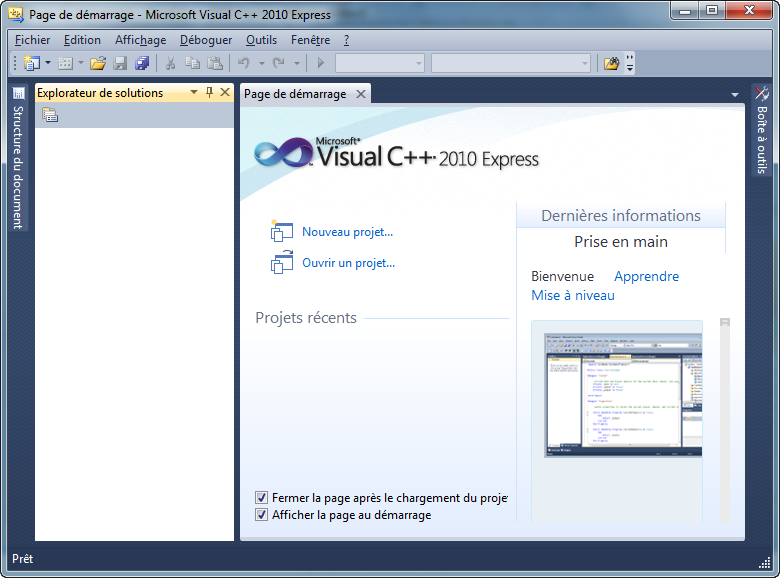
\includegraphics[width=\textwidth]{Chapter_I-2_Visual-Cpp}
\end{figure}

\begin{question}
ما الفرق بين هذه النسخة و النسخة "الحقيقيّة" ؟
\end{question}

لا تحتوي على محرّر موارد يسمح لك برسم الصور، الأيقونات أو النوافذ. هذا لا يهمّنا لأنّنا لن نحتاج إلى هذه الوظائف في هذا الكتاب. وجود هذه الوظائف أمر مستحسن لكنّه ليس لازما.

للتنزيل، زر موقع
\textenglish{Visual C++}.

\url{https://msdn.microsoft.com/fr-fr/express/aa975050.aspx}

و اختر تنزيل
\textenglish{Community 2015}
و اختر لغتك المفضّلة.

\subsection{التثبيت}

التثبيت سهل. سوف يقوم البرنامج بتحميل آخر نسخة من الأنترنت تلقائيا.\\
أنصحك بترك الخيارات كما هي.

بعد ذلك سيطلب منك التسجيل في غضون 30 يوما. لا تقلق، إنه سريع و مجاني لكن يجب القيام بذلك.

اضغط على الرابط المُعطى لك، ستدخل موقع
\textenglish{Microsoft}.
سجّل دخولك باستخدام
\textenglish{Windows Live ID}
(المكافئ لحساب
\textenglish{Hotmail}
أو
\textenglish{MSN})
أو قم بإنشاء واحد إذا لم يكن لديك، ثم أجب بعد ذلك على الأسئلة.

سيتم إعطاؤك في النهاية مفتاح تفعيل. انسخ هذا المفتاح في القائمة
\InlineCode{?}
ثم
"تسجيل المنتج".

\subsection{إنشاء مشروع جديد}

لإنشاء مشروع جديد، إذهب إلى قائمة
"ملف"
(\InlineCode{File})
ثمّ
"جديد"
(\InlineCode{New})
ثم
"مشروع"
(\InlineCode{Project}).
اختر
\InlineCode{Win32}
في العمود الأيسر ثمّ
\InlineCode{Win32 Console Application}.
ثمّ أدْخِل اسم مشروعك.

\begin{figure}[H]
	\centering
	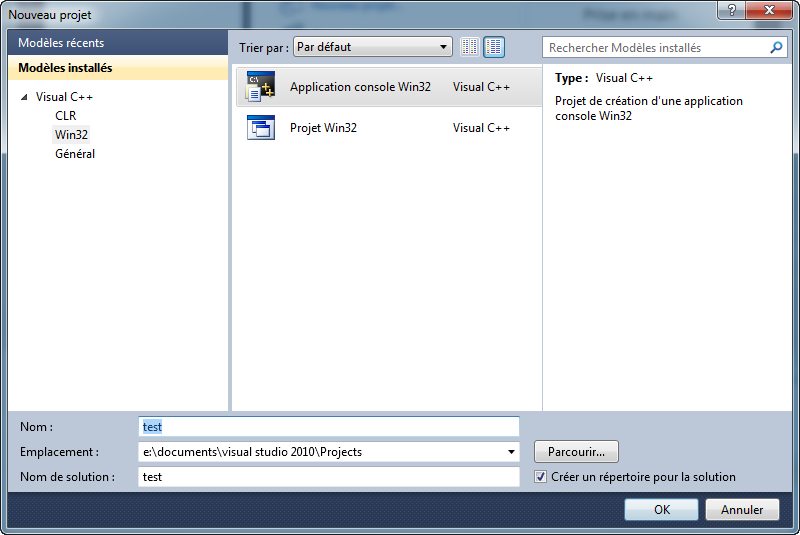
\includegraphics[width=0.8\textwidth]{Chapter_I-2_Visual-Cpp-New-project}
\end{figure}

وافق، ستظهر لك نافذة جديدة.

\begin{figure}[H]
	\centering
	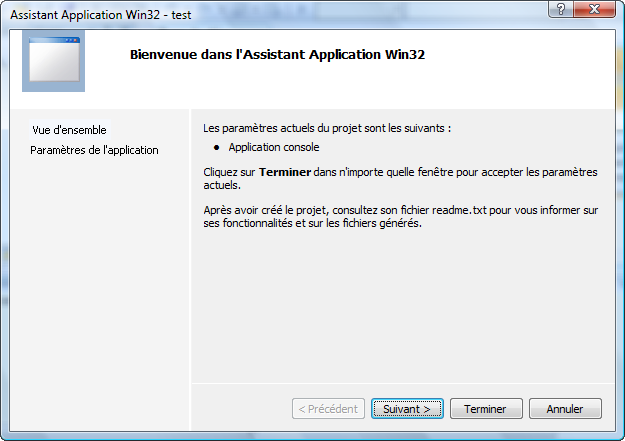
\includegraphics[width=0.8\textwidth]{Chapter_I-2_Visual-Cpp-Welcome}
\end{figure}

هذه النافذة لا تحوي أيّ شيء مهمّ، تابع فقط.

\begin{figure}[H]
	\centering
	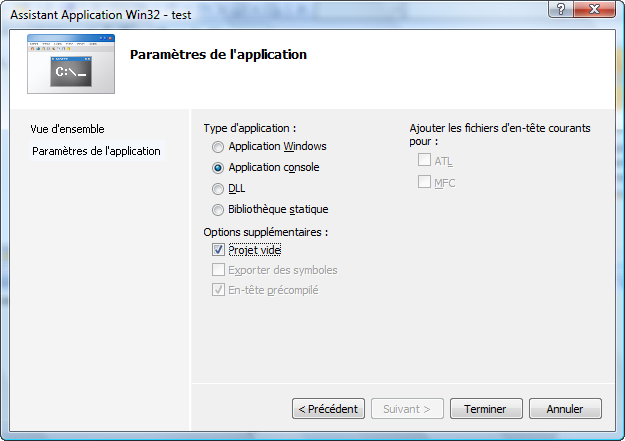
\includegraphics[width=0.8\textwidth]{Chapter_I-2_Visual-Cpp-Parameters}
\end{figure}

اختر
\InlineCode{Console application}
و تأكّد من إنشاء مشروع فارغ عن طريق تحديد
\InlineCode{Empty project}،
ثم اضغط على
"إنهاء"
(\InlineCode{Finish}).

\subsection{إضافة ملف مصدري جديد}

مشروعك فارغ لحدّ الآن. لإضافة ملف مصدري، اضغط باليمين على
"الملفات المصدرية"
(\InlineCode{Source files})
الموجود على اليسار، ثمّ اختر
"إضافة"
(\InlineCode{Add})
ثمّ
"عنصر جديد"
(\InlineCode{New element}).

\begin{figure}[H]
	\centering
	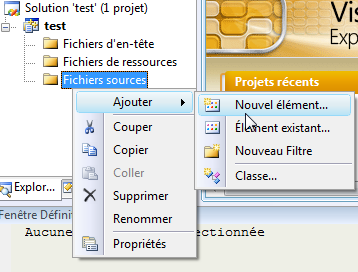
\includegraphics[width=0.5\textwidth]{Chapter_I-2_Visual-Cpp-New-source}
\end{figure}

اختر
\InlineCode{Visual C++}
على اليسار ثمّ
\InlineCode{C++ File}
(أعلمُ أنّنا لا ندرس
\textenglish{C++}
و لكن ليس لهذا أهميّة هنا). أدْخِل اسم الملف :
\InlineCode{main.c}

\begin{figure}[H]
	\centering
	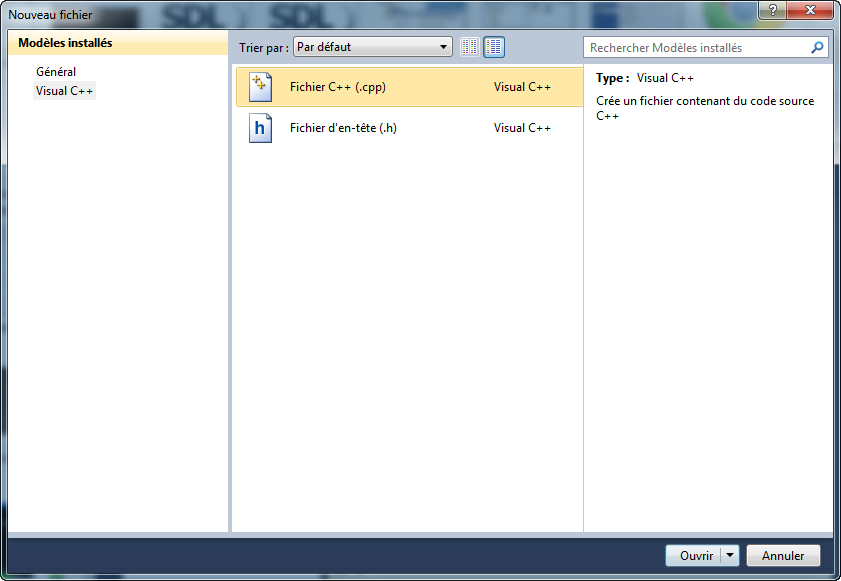
\includegraphics[width=0.8\textwidth]{Chapter_I-2_Visual-Cpp-New-file}
\end{figure}


ثم اضغط على
"إضافة"
(\InlineCode{Add}).
سيتم إنشاء ملفّ فارغ. أنصحك بحفظه بسرعة باسم
\InlineCode{main.c}.

انتهى، يمكنك الآن أن تبدأ في كتابة الشفرة.

\subsection{النافذة الرئيسيّة}

لنرى ما هي أهمّ أقسام النافذة الرئيسيّة في
\textenglish{Visual C++ Express}.

\begin{figure}[H]
	\centering
	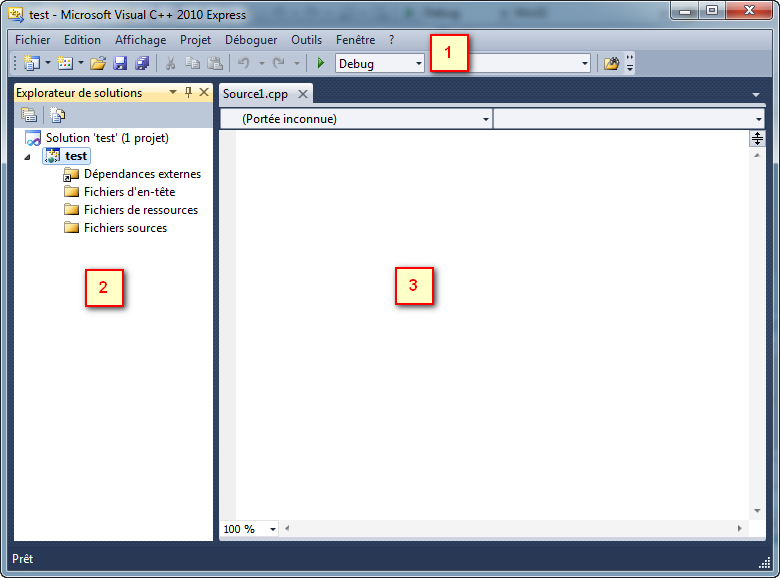
\includegraphics[width=\textwidth]{Chapter_I-2_Visual-Cpp-main}
\end{figure}

هذه النافذة تشبه مثيلتها في
\textenglish{Code::Blocks}.
و لكن رغم ذلك سوف نعيد رؤية معنى كلّ جزء.

\begin{enumerate}
  \item شريط الأدوات : فيه أزرار اعتيادية. لكن كما ترى لا يوجد أيّ زرّ للترجمة. يمكنك إضافته عن طريق النقر باليمين على هذا الشريط و اختيار
"تنقيح"
(\InlineCode{Debug})
و
"توليد"
(\InlineCode{Generate})
من القائمة.

كلّ هذه الأزرار لديها ما يكافئها في القوائم
\InlineCode{Debug}
و
\InlineCode{Generate}.
استخدام
\InlineCode{Generate}
ينشئ الملف التنفيذي (أي أنها تعني الترجمة). إذا استخدمت
\InlineCode{Debug / Execute}
فسوف يقترح عليك الترجمة قبل التشغيل. إختصارات لوحة المفاتيح :
\InlineCode{F7}
لتوليد المشروع و
\InlineCode{F5}
لتشغيله.
  \item هذه المساحة جدّ مهمّة، إذ أنها تحتوي على الملفات الخاصة بمشروعك. أنقر على
"مستكشف الحلول"
(\InlineCode{Solution explorer})
في الأسفل إن لم يكن فُعِل من قبل. سوف ترى أنّه قد تمّ إنشاء مجلّدات لفصل أنواع الملفّات المختلفة (مصدريّة، رأسيّة و موارد). سنتعرف لاحقا على مختلف أنواع الملفات التي تكوّن المشروع.
  \item المساحة الرئيسية : التي نعدّل فيها الملفّات المصدريّة.
\end{enumerate}

أكملنا جولتنا في
\textenglish{Visual C++}.
يمكنك إلقاء نظرة على
الخيارات
إن أردت لكن لا تأخذ من وقتك ثلاث ساعات هناك ! لأنه يوجد كثير منها.

\section{\textenglish{Xcode} (\textenglish{Mac OS X} فقط)}

هناك الكثير من البيئات التطويرية المتوافقة مع
\textenglish{Mac}
على غرار
\textenglish{Code::Blocks}
طبعا.\\
سأقدم لك البيئة الأكثر شهرة في الماك و هي
\textenglish{Xcode}.

\subsection{\textenglish{Xcode}،
 أين أنت ؟}

أغلب مستخدمي
\textenglish{Mac OS X}
ليسوا مبرمجين. لقد فهمت
\textenglish{Apple}
هذا، لذلك لم تثبّته افتراضيا مع النظام.\\
لحسن الحظ، لكلّ من يريد أن يبرمج، كلّ شيء جاهز.
\textenglish{Xcode}
متوفّر على
\textenglish{MacAppStore}.
ابدأ بأخذه من هناك.

أنصحك أيضا بإلقاء نظرة على الموقع الخاص بالمطوّرين لـ\textenglish{Apple}.

\url{https://developer.apple.com/}

سوف تجد هناك كمّا هائلا من من المعلومات المهمّة للتطوير على
\textenglish{Mac}.
يمكنك منه تحميل العديد من البرامج للتطوير.\\
لا تتردّد في التسجيل في
\textenglish{ADC} (\textenglish{Apple Development Connection})،
إنه مجاني و يساعدك على تتبع كل ما هو جديد.

\subsection{تشغيل \textenglish{Xcode}}

أوّل شيء يمكننا فعله هو إنشاء مشروع جديد، فلنبدأ بهذا. إذهب إلى
"ملف "
(\InlineCode{File})
ثمّ
"مشروع جديد"
(\InlineCode{New Project}).
ستفتح لك نافذة اختيار المشروع.

\begin{figure}[H]
	\centering
	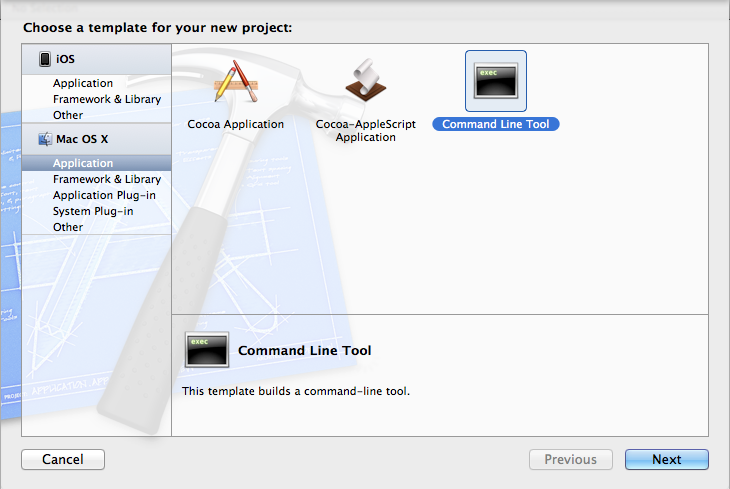
\includegraphics[width=0.8\textwidth]{Chapter_I-2_Xcode-New-project}
\end{figure}

اختر
\InlineCode{Application}
من اليسار ثمّ
\InlineCode{Command Line Tool}.
اضغط بعدها على
\InlineCode{Next}.
سوف يُطلب منكم بعدها حفظ مشروعك (كلّ مشروع يجب أن يحفظ منذ البداية) و اسمه. ضعه في المجلّد الّذي تريد.

بمجرّد إنشائه، سيتّم عرض مشروعك على شكل مجلّد يحتوي على العديد من الملفّات في الـ\InlineCode{Finder}.
الملف الّذي يملك الامتداد
\InlineCode{.xcodeproj}
يوافق ملف المشروع. إنه الملف الذي عليك اختياره في المرة القادمة لفتح مشروعك.

\subsection{نافذة التطوير}

في
\textenglish{Xcode}،
عندما تختار
\InlineCode{main.c}
تظهر لك نافذة شبيهة بهذه :

\begin{figure}[H]
	\centering
	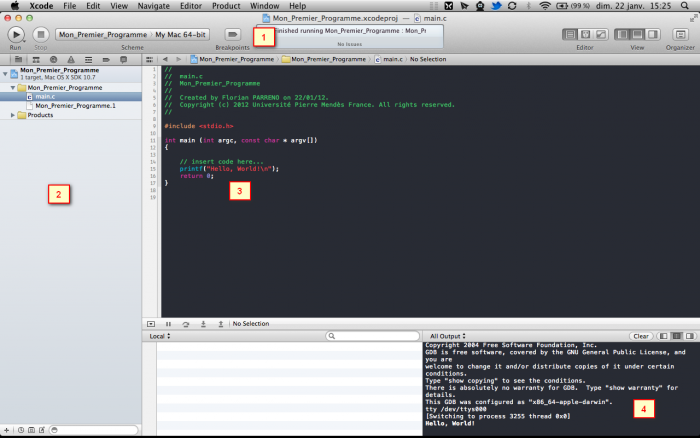
\includegraphics[width=\textwidth]{Chapter_I-2_Xcode-main}
\end{figure}

الواجهة مقسمة إلى أربعة أقسام، مرقمة هنا من 1 إلى 4 :

\begin{enumerate}
  \item الجزء الأوّل هو شريط الأزرار في الأعلى. أهمّ زرّ فيه هو
"تشغيل"
(\InlineCode{Run})
وظيفته تشغيل البرنامج.
  \item الجزء اليسار مخصص للتمثيل الشُجيري لمشروعك الخاص. بعض الأقسام تحتوي على الأخطاء، التحذيرات، إلخ. يقوم
\InlineCode{Xcode}
تلقائيّا بنقلك إلى القسم المهم. و هو الذي يحمل اسم المشروع.
  \item الجزء الثالث تتغيّر وظيفته حسب ما قمت بتحديده في الجزء الأيسر. و هنا يعرض محتوى الملف
\InlineCode{main.c}.
  \item أخيرا، الجزء الرابع يُظهر نتائج تشغيل البرنامج على الشاشة عندما تقوم بتشغيل البرنامج.
\end{enumerate}

\subsection{إضافة ملفّ جديد}

في البداية، لن تملك سوى ملف مصدري واحد و هو
\InlineCode{main.c}،
و لكن لاحقا عندما نتقدم في الدروس سأطلب منك إنشاء ملفات مصدريّة بنفسك، عندما تصبح برامجنا أكبر.

لإنشاء ملفّ جديد، اذهب إلى قائمة
\InlineCode{File}
ثمّ
\InlineCode{New File}.
سيطلب منك إدخال نوع الملف الذي تريد إنشاءه. توجّه إلى قائمة
\InlineCode{Mac OS X}
و اختر
\InlineCode{C and C++}
ثمّ
\InlineCode{C File}.
لاحظ هذه الصورة.

\begin{figure}[H]
	\centering
	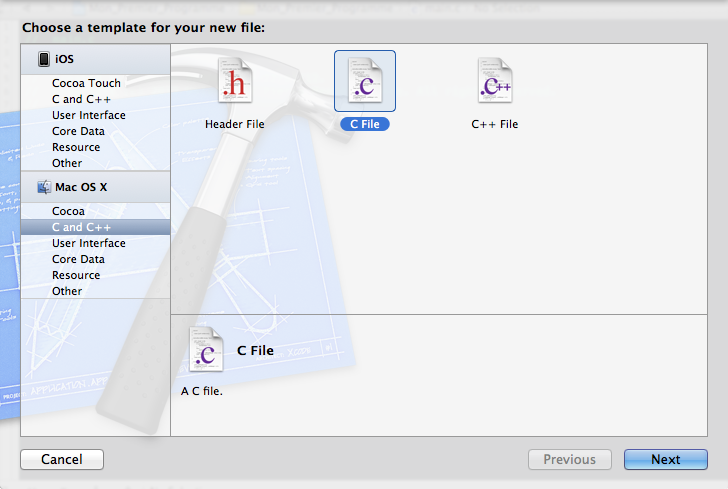
\includegraphics[width=0.8\textwidth]{Chapter_I-2_Xcode-C}
\end{figure}

يجب عليك إعطاء اسم لملفّك الجديد. امتداده يجب أن يبقى
\InlineCode{.c}.
أحيانا -كما سنرى لاحقا- يجب عليك أيضا إنشاء ملفّات بامتداد
\InlineCode{.h}.
الخانة
\InlineCode{Also create file.h}
مخصّصة لهذا الغرض. حاليّا هذا الخيار لا يهمّنا.

انقر بعدها على
\InlineCode{Finish}.
انتهى ! أصبح في مشروعك ملفٌ آخر غير الملف
\InlineCode{main.c}،
هنيئا لك فقد أصبحت الآن جاهزاً للبرمجة على الـ\InlineCode{Mac}.

\section*{ملخّص}

\begin{itemize}
  \item المبرمجون يحتاجون إلى ثلاثة أدوات : محرّر نصوص، مترجم و منقّح.
  \item من الممكن تثبيت هذه الأدوات منفصلة، لكنّه من المعتاد البوم الحصول على حُزمةٍ ثلاثة-في-واحد نسميها بيئة التطوير المتكاملة.
  \item \textenglish{Code::Blocks}،
\textenglish{Visual C++}،
و
\textenglish{Xcode}
تعدّ من بين بيئات التطوير الأكثر شهرة.
\end{itemize}

  \chapter{برنامجك الأوّل}

لقد قمنا بتحضير كلّ شيء إلى حد الآن ويمكننا أن نبدأ قليلا من البرمجة. مع نهاية هذا الفصل ستكون قد نجحت في إنشاء أوّل برنامج لك.

لكي أصدقك القول، سيظهر البرنامج بالأبيض والأسود ولن يقوم بشيء سوى إلقاء التحيّة. يبدو عديم الفائدة، لكنّه برنامجك الأوّل وأؤكّد لك أنّك ستكون فخورا به.

\section{كونسول أو نافذة ؟}

لقد تحدثنا سابقا عن فكرة برامج الكونسول وبرامج النوافذ في الفصل السابق. البيئة التطويرية تطلب منا تحديد أي نوع من البرامج نريد أن ننشئها. ولقد قلنا إننا سننشئ برامج من نوع كونسول.

يوجد نوعان من البرامج، لا أكثر :

\begin{itemize}
  \item ،برامج بنوافذ
  \item برامج تعمل في الكونسول.
\end{itemize}

\subsection{البرامج الّتي تملك نوافذ}

هي البرامج التي نعرفها جميعا. هذا مثال على برنامج من نوع نافذة، مثل الرسام.

\begin{figure}[H]
	\centering
	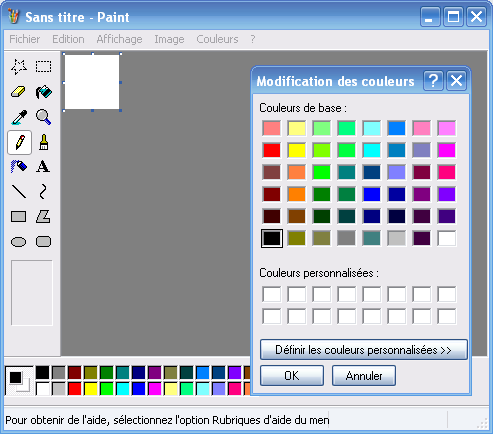
\includegraphics[width=0.6\textwidth]{Chapter_I-3_Paint}
\end{figure}

أعتقد أنّك تحب إنشاء برامج كهذه، لكنّ هذا ليس في مقدورك حاليا. في الواقع، إنشاء برامج بنوافذ هو أمر ممكن بلغة \textenglish{C}، لكنّ بالنسبة لمبتدئ، هذا أمر معقّد جدّا. كبداية، يستحسن إنشاء برامج الكونسول.

\begin{question}
  لكن ماذا يعنى برنامج
\textenglish{Console}
؟
\end{question}

\subsection{البرامج الّتي تعمل في الكونسول}

برامج الكونسول هي أول ما ظهر من برامج. في ذلك الوقت، شاشات الحواسيب لم تكن سوى بالأبيض والأسود، ولم تكن فعّالة لكي تتمكّن من رسم النوافذ كما هو الحال مع حواسيبنا حاليّا.

مرّ الزمن بسرعة وزادت شعبية الويندوز نظراً لبساطته إلى أن نسي كثير من الناس ما هي الكونسول.

لديّ خبر جيّد لك !
\textbf{الكونسول لم تمت بعد} !
 في الواقع،
\textenglish{GNU/Linux}
 قد أعاد الكونسول إلى الحياة. هذه صورة لكونسول على
\textenglish{GNU/Linux}.

\begin{figure}[H]
	\centering
	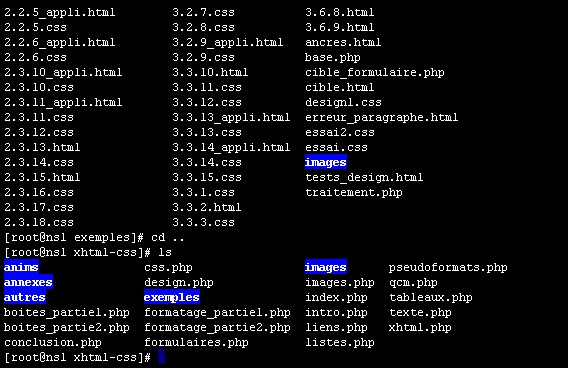
\includegraphics[width=0.6\textwidth]{Chapter_I-3_Console}
\end{figure}

مرعب ! صحيح ؟ لكن على الأقل عرفت ما هي الكونسول، وهذه بعض الملاحظات :

\begin{itemize}
  \item اليوم، يمكننا عرض الألوان في الكونسول. ليس كلّ شيء بالأبيض والأسود كما تتخيّل.
  \item الكونسول هو الأسهل من ناحية البرمجة بالنسبة للمبتدئين.
  \item أداة عالية الإمكانيّات إذا عرفنا كيف نستخدمه.
\end{itemize}

كما قلت لك، إنشاء برامج كونسول أمر سهل جدّا وملائم للمبتدئين (وهذا عكس برامج النوافذ). ليكن في علمك أيضا أنّ الكونسول قد تطوّرت وبإمكانها عرض الألوان، ولا شيء يمنعك من إضافة صورة خلفيّة لها.

\begin{question}
  وفي الويندوز ألا توجد
\textenglish{Console}
 ؟
\end{question}

بلى، لكنّها مخفيّة لو صح القول. يمكنك فتحها بالذهاب إلى "إبدأ"
(\InlineCode{Start})
 ثمّ "ملحقات"
(\InlineCode{Accessories})
 ثمّ "موجه الأوامر"
(\InlineCode{Command prompt})
 أو بالذهاب إلى "إبدأ" ثمّ "تشغيل"
(\InlineCode{Run})
 واكتب فيها
\InlineCode{cmd}
 واضغط على "موافق".

\begin{figure}[H]
	\centering
	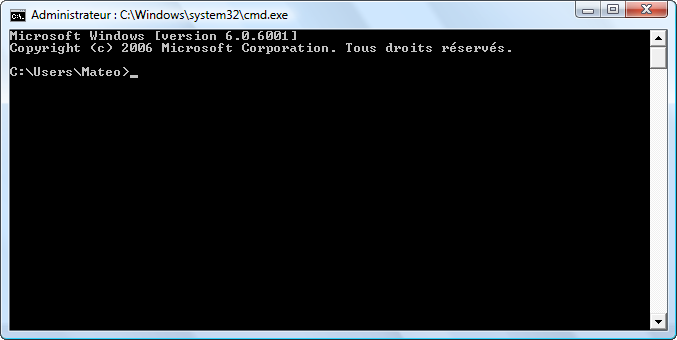
\includegraphics[width=0.6\textwidth]{Chapter_I-3_Console-Windows}
\end{figure}

إذا كنت تستخدم نظام ويندوز، فاعلم بأن أولى برامجك ستكون في نوافذ شبيهة بهذه. أنا لم أختر البداية هكذا لجعلك تشعر بالملل، بل لتعليمك الأساسيّات اللازمة لكي تتمكّن لاحقا من إنشاء النوافذ.

إذن فلتكن متيقّناً، بمجرّد أن تصل إلى المستوى اللازم لإنشاء النوافذ، سوف أعلّمك كيف تفعل ذلك.

\section{الحدّ الأدنى من الشفرة المصدرية}

من أجل أي برنامج، يجب كتابة قدر معيّن من الشفرة المصدرية. هذه الشفرة لا تقوم بشيء خاصّ لكنّها ضروريّة. هذه الشفرة التي سنكتشفها الآن ستكون أساس أغلب برامجك الّتي ستكتبها بلغة \textenglish{C}.

\subsection{أطلب من البيئة التطويرية الخاصة بك تزويدك بالحد الأدنى من الشفرة المصدرية}

لقد لاحظت أن طريقة إنشاء مشروع جديد تختلف من بيئة تطويرية إلى أخرى. إليك تذكيراً بسيطا : في برنامج
\textenglish{Code::Blocks}
 (الذي سنستخدمه في هذا الكتاب)، عليك التوجه نحو
\InlineCode{File}
 ثمّ
\InlineCode{New}
 ثمّ
\InlineCode{Project}
 ثم تختار
\InlineCode{Console Application}
 وبعدها اللغة
\textenglish{C}.
سيولّد لك الحد الأدنى من الشفرة المصدرية
 \textenglish{C}
 التي تحتاجها. ها هي :

\begin{Csource}
#include <stdio.h>
#include <stdlib.h>

int main()
{
    printf("Hello world!\n");
    return 0;
}

\end{Csource}

\begin{information}
لاحظ أنّه يوجد سطر فارغ في نهاية الشفرة. يفترض أن ينتهي كل ملف مكتوب بلغة
\textenglish{C}
هكذا. إن لم تفعل ذلك، فهذه ليست بمشكلة، لكن توقّع أن يعرض لك المترجم تحذيراً
(\textenglish{Warning}).
\end{information}

علماً أنّ السطر :
\begin{Csource}
int main()
\end{Csource}
\dots
بإمكانه أن يُكتب كالتالي :

\begin{Csource}
int main(int argc, char *argv[])
\end{Csource}

كلتا العبارتين تحملان نفس المعنى لكن الثانية، الأكثر تعقيدا، هي الأكثر شيوعا، لذلك فإنّنا سنستخدمها في الفصول القادمة.\\
إستخدامنا للشكل الأوّل أو الثاني لا يغيّر شيئا بالنسبة لنا. لذلك لا داعي لإضاعة الوقت هنا، خصوصاً أنّك لا تملك المستوى اللازم لفهم ما تعنيه.

إذا كنت تستخدم بيئة تطويرية أخرى فقم بنسخ هذه الشفرة المصدرية وألصقها في الملف \InlineCode{main.c} ليكون لديكم نفس الشفرة.

أخيرا، قم بحفظ عملك في المشروع. أعلم أننا لم نقم بشيء حتّى الآن لكن من الجيّد التعوّد على الحفظ في كلّ مرّة.

\subsection{تحليل أسطر الشفرة المصدرية السابقة}
قد تبدو لك الشفرة المصدرية السابقة أنّها كاللغة الصينيّة، أنا أتخيّل ذلك ! في الواقع هي تسمح بإنشاء برنامج كونسول يعرض نصّا على الشاشة. يجب تعلّم كيفيّة قراءة كلّ هذا.

فلنبدأ بأوّل سطرين :
\begin{Csource}
#include <stdio.h>
#include <stdlib.h>
\end{Csource}

هذان السطران يبدآن بعلامة
\InlineCode{\#}.
وهي أسطر خاصّة تُعرف باسم
\textbf{توجيهات المعالج القبلي}
(\textenglish{Preprocessor directives}). اسم معقّد، أليس كذلك ؟ هذه الأسطر تتمّ قراءتها من طرف البرنامج المسمّى بالمعالج القبلي، وهو برنامج يتمّ تشغيله في بداية الترجمة.

ما رأيناه سابقا كان مخطّطا بسيطا لعمليّة الترجمة. لكنّ في الواقع، هناك الكثير من المراحل التي تحدث في هذه العمليّة. سنقوم بتفصيل هذا لاحقا. حاليّا عليك فقط تذكّر وضع هذين السطرين أعلى كلّ ملفّاتك.

\begin{question}
  حسنا لكن ماذا يعنيه هذان السطران ؟ أريد أن أعرف !
\end{question}

كلمة
 \InlineCode{include}
 بالإنجليزيّة تعني "تضمين". هذان السطران يقومان بتضمين ملفّات في المشروع، أي إضافة هذه الملفّات من أجل عمليّة الترجمة. هناك سطران وبالتالي هناك ملفان يتمّ تضمينهما في المشروع وهما بالترتيب :
\InlineCode{stdio.h}
 و
\InlineCode{stdlib.h}.
هذان الملفّان موجودان بالفعل على حاسوبك وهما ملفّان مصدريّان جاهزان، سوف تعرف مستقبلا أنّنا نسميها
\textbf{مكتبات}
(\textenglish{Libraries}).
 هذه الملفّات تحتوي الشفرة المصدرية اللازمة لعرض نصّ على الشاشة.

 بدون هذين الملفّين، كتابة نصّ على الشاشة سيكون أمرا مستحيلاً. فالحاسوب لا يعرف فعل أي شيء مبدئيا.

 باختصار، السطران الأول والثاني يقومان بتضمين المكتبات التي ستساعدنا في إظهار نصّ على الشاشة بكلّ سهولة.

 نمر للتالي، باقي الأسطر :
 
\begin{Csource}
int main()
{
    printf("Hello world!\n");
    return 0;
}
\end{Csource}

ما تراه هنا هو ما نسميه بـ\textbf{التابع}
أو
\textbf{الدالّة}
(\textenglish{Function}).
 البرنامج في لغة
\textenglish{C}
 يتكوّن من مجموعة دوال. حاليّا برنامجنا لا يحوي سوى دالّة واحدة.

الدالّة تمكّننا من تجميع مجموعة من الأوامر. الغرض من تجميع الأوامر هو جعلها تقوم بوظيفة ما. مثلا يمكننا إنشاء دالّة باسم
 \InlineCode{open\_file}
 وجعلها تحتوي التعليمات التي تشرح للحاسوب كيفيّة فتح ملف.

 دون الدخول في تفاصيل إنشاء الدالّة (الوقت مبكّر، سوف نتحدّث عن الدوال في وقت لاحق) لنحلّل رغم ذلك أجزائه الكبيرة. السطر الأوّل يحتوي اسم الدالّة، إنّه الكلمة الثانية.\\
 أجل، اسم دالّتنا هو
\InlineCode{main}
والذي يعني
"الرئيسية"
. وتشغيل البرنامج دائما يبدأ من الدالة
\InlineCode{main}.

للدالّة بداية ونهاية، وهي محدودة بالحاضنتين
\InlineCode{\{}
و
\InlineCode{\}}.
محتوى الدالّة موجود بين هاتين الحاضنتين. إن كنت قد تابعت جيداً فقد عرفت أنّ الدالّة مشكّلة من سطرين :

\begin{Csource}
printf("Hello world!\n");
return 0;
\end{Csource}

هاته الأسطر في الداخل نسميها
\textbf{التعليمات}
(\textenglish{Instructions})
 (هذه إحدى المصطلحات الّتي يجب عليك حفظها). كلّ تعليمة تمثّل أمراً بالنسبة للحاسوب. فكلّ واحدة منها تطلب منه فعل شيء محدّد.

 كما قلت لك، بتجميع ذكيّ للتعليمات في الدالّة يمكننا إنشاء أجزاء برنامج جاهزة للاستخدام. باستخدام التعليمات المناسبة يمكننا إنشاء دالّة
 \InlineCode{open\_file}
 كما شرحت لك قبل قليل، و أيضا دالّة
\InlineCode{move\_character}
 في لعبة فيديو، على سبيل المثال.

 البرنامج في الواقع ما هو إلّا تتابع لتعليمات : إفعل هذا و إفعل ذاك. أنت تعطي أوامر للحاسوب و هو يقوم بتنفيذها.

 \begin{critical}
هامّ جدّا : لا بدّ أن تنتهي كلّ تعليمة بفاصلة منقوطة
"\InlineCode{;}"
. بهذا يمكن التفريق بين ما إذا كانت هذه تعليمة أم لا. إذا نسيت وضع فاصلة منقوطة نهاية تعليمة ما، فلن تتمّ ترجمة برنامجك.
 \end{critical}

 السطر الأول :
 \InlineCode{printf("Hello world!\\n");}
 يطلب إظهار الرسالة
 "\textenglish{Hello world!}"
  على الشاشة. عندما يصل برنامجك إلى هذا السطر، فسوف يقوم بعرض هذه الرسالة ثمّ المرور إلى التعليمة التالية.

  التعليمة التالية هي
\InlineCode{return 0;}
 و هي تخبرنا أنّ الدالّة
\InlineCode{main}
 قد انتهت و تطلب منه إعادة 0.

 \begin{question}
   لماذا يقوم برنامجي بإعادة العدد 0 ؟
 \end{question}

 في الواقع، كلّ برنامج عندما ينتهي يُرجع قيمة معينة. على سبيل المثال، ليقول أنّ كلّ شيء سار على ما يرام. عمليّا، 0 يعني  أنّ كلّ شيء سار على ما يرام، و كلّ قيمة أخرى تدلّ على حدوث خطأ. في أغلب الأحيان هذه القيمة لا تُستخدم ، لكن يجب رغم ذلك استعمالها.\\
 كان يمكن أن يعمل برنامجك بدون
 \InlineCode{return 0}
، لكن يمكننا القول أن وضعها يعتبر أمراً أكثر نظافة و أكثر جدّية.

إلى هنا نكون قد فصّلنا قليلا في عمل هذه الشفرة المصدرية.

طبعا، نحن لم ندرس كلّ شيء بعمق، و قد تكون لديك بعض الأسئلة عالقة في ذهنك. كن على يقين بأنك ستجد لها أجوبة شيئا فشيئا مع تقدّمنا في الكتاب. لا يمكنني أن أطلعك على كلّ شيء من البداية، لأنّ هناك كثيراً من الأشياء لاستيعابها.

إليك ما يلي : بما أنني في حال جيّدة، سأقوم بوضع مخطّط يضمّ المصطلحات الّتي تعلّمناها في هذا الفصل.

\begin{figure}[H]
	\centering
	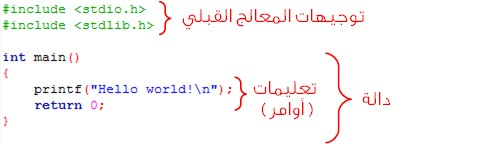
\includegraphics[width=0.8\textwidth]{Chapter_I-3_HelloWorld}
\end{figure}

\subsection{لنجرّب برنامجنا}

كلّ ما سنقوم به الآن هو ترجمة المشروع ثمّ تشغيله (اضغط على
\InlineCode{Build \& Run}
 إذا كنت على
\textenglish{Code::Blocks}).
سيطلب منك حفظ مشروعك إذا لم تقم بذلك من قبل.

\begin{critical}
  إن لم تنجح الترجمة و ظهر لك خطأ مثل :\\
\InlineCode{"My-program - Release" uses an invalid compiler. Skipping...}\\\InlineCode{Nothing to be done...}
فهذا يعني أنّك نزلت نسخة
\textenglish{Code::Blocks}
 دون
\InlineCode{mingw}
 (المترجم)، عد و نزّل النسخة التي تحتوي على
\InlineCode{mingw}.
\end{critical}

بعد بُرهة، يظهر برنامجك كما في الصورة :

\begin{figure}[H]
	\centering
	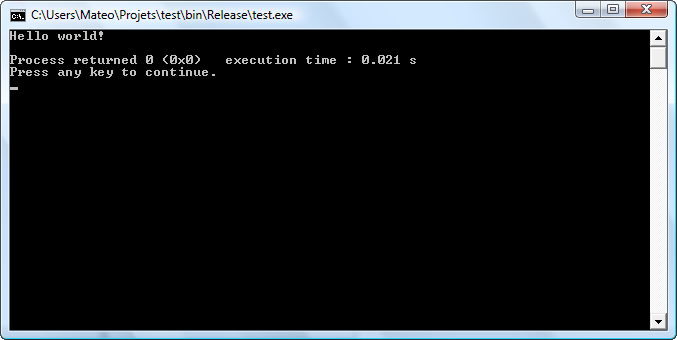
\includegraphics[width=0.8\textwidth]{Chapter_I-3_HelloWorld-run}
\end{figure}

البرنامج يُظهر
"\textenglish{Hello world!}"
 (في السطر الأوّل).\\
الأسطر الّتي أسفله تمّ توليدها من طرف
\textenglish{Code::Blocks}
 وتدلّ على أنّ البرنامج قد تمّ تشغيله بنجاح كما أنها تعطي الوقت الذي استغرقه البرنامج في التشغيل.

 سيطلب منك الضغط على إحدى المفاتيح لإغلاق النافذة. أعلم أن الأمر لم يكن ممتعا جدّا. لكنه برنامجك الأوّل، وهذه لحظة ستتذكرها طيلة حياتك ! ألا تعتقد ذلك ؟

\section{كتابة رسالة على الشاشة}

من الآن سنقوم بإدخال التعديلات على الشفرة المصدرية السابقة. مهمّتك، إن قبلتها : عرض رسالة
"\textenglish{Bonjour}"
 على الشاشة.

\begin{question}
  كيف يمكنني اختيار النص الّذي سيظهر على الشاشة ؟
\end{question}

الأمر بسيط جدا، إذا بدأت من الشفرة التي رأيناها سابقاً، فسيكون عليك استبدال
"\textenglish{Hello world!}"
 بـ"\textenglish{Bonjour}"
 في السطر الذي يستدعي
\InlineCode{printf}.

كما قلت من قبل،
\InlineCode{printf}
 هي
\textbf{تعليمة}
 وهي تعطي أمراً للحاسوب : "قم بعرض هذه الرسالة على الشاشة".\\
يجب أن تعرف أيضا أن
\InlineCode{printf}
 هي دالّة كُتِبَت من قبل من طرف مبرمجين قبلك.

\begin{question}
   أين توجد هذه الدالّة ؟ أنا لا أرى سوى الدالّة \InlineCode{main} !
\end{question}

هل تذكر هذين السطرين ؟

\begin{Csource}
#include <stdio.h>
#include <stdlib.h>
\end{Csource}

قلت لك من قبل أنهما يمكنان البرنامج من إضافة مكتبات. المكتبات في الحقيقة هي ملفّات تحوي أطنانا من الدوال جاهزة للإستخدام. هذه الملفات
(\InlineCode{stdio.h} و \InlineCode{stdlib.h})
 تحوي أغلب الدوال الأساسية التي قد نحتاجها في برنامج ما.
\InlineCode{stdio.h}
 بحد ذاته يحوي دوال تمكّن من عرض أشياء على الشاشة (مثل
 \InlineCode{printf})
 و أيضا الطلب من المستخدم إدخال شيء ما (هذه دوال سنتعرّف عليها لاحقا).

\subsection{لنقل مرحبا للسيّد}

في دالّتنا
\InlineCode{main}
نستدعي الدالّة
 \InlineCode{printf}.
 أي أن لدينا دالّة تستدعي أخرى (هنا
\InlineCode{main}
تستدعي
\InlineCode{printf}).
سترى أن هذا ما يحدث دائما في لغة
\textenglish{C}
: دالّة تحتوي تعليمات تستدعي دوال أخرى، وهكذا.

إذن، لاستدعاء دالّة يكفي كتابة اسمها متبوعا بقوسين، ثم فاصلة منقوطة.

\begin{Csource}
printf();
\end{Csource}

هذا جيد، لكنه غير كاف. يجب أن نُعلم البرنامج بما يجب أن يكتبه في الشاشة. لفعل هذا يجب أن نعطي
\InlineCode{printf}
النص المطلوب عرضه. لفعل هذا نقوم بوضع النص داخل علامات الإقتباس المزدوجة بين القوسين.\\
في حالتنا هذه سنكتب تماما :

\begin{Csource}
printf("Bonjour");
\end{Csource}

آمل ألا تكون قد نسيت رمز الفاصلة المنقوطة في النهاية، وأذكّرك أنّها مهمّة جدا لأنّها تدلّ على نهاية التعليمة.\\
هذه هي الشفرة المصدرية التي يجب أن تحصل عليها :

\begin{Csource}
#include <stdio.h>
#include <stdlib.h>

int main()
{
    printf("Bonjour");
    return 0;
}
\end{Csource}

لدينا إذن تعليمتان تطلبان من الحاسوب القيام بهذين الأمرين بهذا الترتيب :
\begin{enumerate}
  \item عرض
"\textenglish{Bonjour}"
على الشاشة.
  \item نهاية الدالّة
\InlineCode{main}
، إعادة 0. البرنامج يتوقّف.
\end{enumerate}

هذا ما يظهر على شاشتك :

\begin{figure}[H]
	\centering
	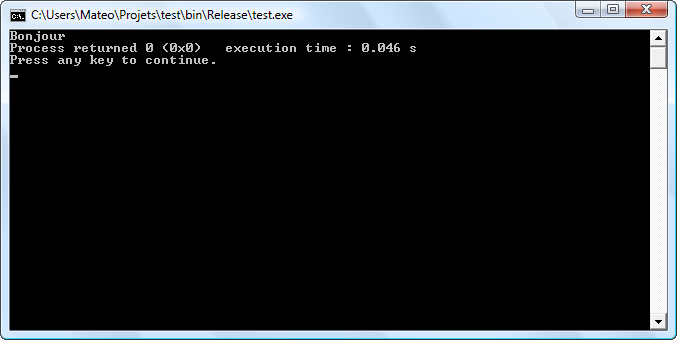
\includegraphics[width=0.8\textwidth]{Chapter_I-3_Good-Morning}
\end{figure}

كما ترى، السطر الذي يحتوي الرسالة يكون ملتصقاً قليلا بباقي النص، على خلاف ما رأيناه سابقا.\\
أحد الحلول الممكنة هو إضافة رمز للعودة إلى السطر بعد
 "\textenglish{Bonjour}"
 (كما لو أنّنا ضغطنا على المفتاح
\InlineCode{Enter}).

ولكن ضغط المفتاح
\InlineCode{Enter}
 في الشفرة المصدرية لن يعمل كما تتوقع، لهذا يجب استخدام المحارف الخاصّة
(\textenglish{Special characters}).

\subsection{المحارف الخاصّة}

المحارف أو الرموز الخاصّة هي محارف تمكّن من تعريف عودة إلى السطر، جدولة، إلخ.\\
من السهل التعرّف عليها، فهي مكوّنة من محرفين. الأوّل هو الشَرْطَةُ المائلة الخلفية 
(\textbackslash) (\textenglish{Backslash})
والثاني يكون رقما أو حرفا. إليك محرفين خاصّين قد تحتاجهما كثيرا :

\begin{itemize}
  \item \InlineCode{\textbackslash n} :
 العودة إلى السطر.
 \item \InlineCode{\textbackslash t} :
 الجدولة (فراغ كبير في نفس السطر).
\end{itemize}

في حالتنا هذه، يكفي أن نكتب
\InlineCode{\textbackslash n}
 لإنشاء العودة إلى السطر. إذن، إذا أردنا أن نضع عودة إلى السطر بعد
\textenglish{Bonjour}
، فيكفي أن نكتب :

\begin{Csource}
printf("Bonjour\n");
\end{Csource}

وسيفهم حاسوبك أنّ عليه كتابة
"\textenglish{Bonjour}"
 ويعود إلى السطر.

\begin{figure}[H]
	\centering
	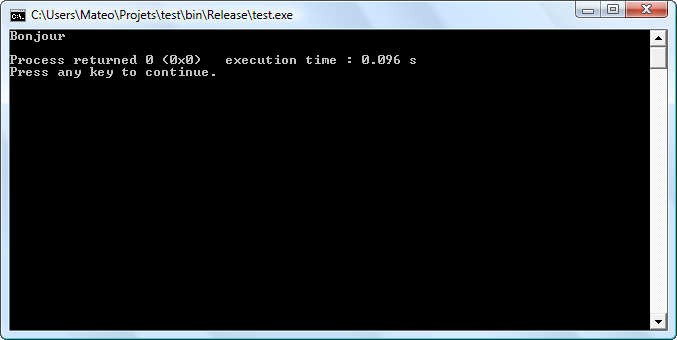
\includegraphics[width=0.8\textwidth]{Chapter_I-3_Good-Morning-backslash-n}
\end{figure}

\begin{information}
  يمكنك الكتابة بعد
\InlineCode{\textbackslash n}
بدون أيّة مشكلة. كلّ ما تكتبه بعد
\InlineCode{\textbackslash n}
 سيوضع في السطر الجديد. يمكنك إذن التدرّب على كتابة :
\InlineCode{printf("Good morning\textbackslash nGood bye\textbackslash n");}\\
و سيتمّ عرض
"\textenglish{Good morning}"
على السطر الأوّل و
"\textenglish{Good bye}"
على السطر الثاني.
\end{information}

\subsection{متلازمة \textenglish{Gérard}}

\begin{question}
  مرحبا، اسمي
\textenglish{Gérard}
و قد حاولت تعديل برنامجك ليقول
"\textenglish{Bonjour Gérard}"،
و لكنّي ألاحظ أنّ حرف
\textenglish{é}
 لا يظهر بشكل جيّد
\dots
 مالّذي عليّ فعله ؟
\end{question}

أوّلا، مرحبا بك
\textenglish{Gérard}
. هذا سؤال جيّد. لكن لديّ خبر سيّء لك. الكونسول الخاصة بـ\textenglish{Windows}
لا تمكّن من عرض الحروف الّتي تحوي علامات النطق الصوتي مثل
\textenglish{é}
، خلافا لكونسول
\textenglish{GNU/Linux}
التي تفعل. لديّ حلّان لهذه المشكلة :

\begin{itemize}
  \item \textbf{استخدم
\textenglish{GNU/Linux}}
. هذا حلّ جذريّ بعض الشيء. أحتاج إلى درس كامل لأعلّمك كيف تعمل على
\textenglish{GNU/Linux}
. إذا لم يكن لديك المستوى، إنس هذا الخيار حاليّا.
  \item \textbf{لا تستخدم الحروف الّتي تحوي علامات النطق الصوتي}.
للأسف إنّه الحل الّذي قد يكون عليك اختياره. الكونسول الخاصة بـ\textenglish{Windows}
لها عيوبها. يجب عليك التعوّد على عدم كتابة مثل هذه الحروف. لكن مستقبلا قد تنشئ برامج بنوافذ ولن تعاني من هذا المشكل. لذلك أنصحك بالصبر على هذه المشكلة حاليّا، فبرامجك المستقبلية "الاحترافية" لن يكون فيها هذا المشكل.
\end{itemize}

لكيلا تنزعج، يمكنك الكتابة دون استخدام الحروف التي تملك علامات النطق الصوتي :

\begin{Csource}
printf("Bonjour Gerard\n");
\end{Csource}

نشكر صديقنا
\textenglish{Gérard}
لتنبيهنا على هذه المشكلة !

\section{التعليقات، مهمّة جدا !}

قبل ختم هذا الفصل الأوّل "الحقيقي" في البرمجة، يجب أن أعرّفك على
\textbf{التعليقات}
(\textenglish{Comments})
. أيّا كانت لغة البرمجة الّتي تستخدمها، ستكون لديك القدرة على إضافة التعليقات للشفرة المصدرية الخاصة بك.

ولكن ما الذي يعنيه "التعليق"؟\\
هذا يعني إمكانية وضع نصّ في وسط برنامجك لشرح دوره، مثلاً : ما الذي يفعله هذا السطر، إلخ. هذا بالفعل أمر ضروريّ، لأنّه حتّى لو كنت عبقرياً في البرمجة، ستكون بحاجة إلى وضع ملاحظات هنا وهناك. هذا يمكنك من :

\begin{itemize}
  \item العثور على ما تبحث عنه بسهولة في الشفرة المصدرية عندما تعود إليه بعد مدّة. من الطبيعيّ أن ننسى كيف تعمل البرامج الّتي كتبناها بعد مدّة. إن توقّفت عن البرمجة لأيّام ثمّ عدت فستكون بحاجة إلى التعليقات لإيجاد ما تريد في شفرة كبيرة جدّا.
  \item إذا أعطيت مشروعك لأحد غيرك (وهو لا يعرف شيئا عن الشفرة المصدرية الخاصة بك)، فالتعليقات تمكّنه من التآلف مع مشروعك بسرعة.
  \item وأخيرا، ستسمح لي بإضافة شروحات وملاحظات حول الشفرة المصدرية في هذه الدروس. وهذا سيفيدك في فهم ما الذي يعنيه كلّ سطر.
\end{itemize}

توجد طريقتان لإضافة تعليق. وهذا يعتمد على طول التعليق المراد إدراجه :

\begin{itemize}
  \item إذا كان تعليقك
\textbf{قصيرا}
: فيمكن كتابته على سطر واحد، ولا يحتوي سوى كلمات قليلة. في هذه الحالة، عليك كتابة شرطتين مائلتين
(\InlineCode{//})
متبوعين بتعليقك. على سبيل المثال :

\begin{Csource}
// This is a comment.
\end{Csource}

بإمكانك إضافة تعليق وحده على السطر، أو على يمين تعليمة معينة. وهذا أمر مهمّ جدّا، لأنّ بهذه الطريقة يمكننا تحديد ما الذي يعنيه السطر الّذي كُتب بجانبه. مثال :

\begin{Csource}
printf("Bonjour"); // This instruction displays 'Bonjour' on the screen
\end{Csource}

  \item  إذا كان تعليقك
\textbf{طويلا}:
لديك الكثير لتقوله، تريد كتابة الكثير من الجمل على كثير من الأسطر. في هذه الحالة، يجب عليك كتابة شفرة تشير إلى "بداية التعليق" وأخرى تشير إلى "نهاية التعليق":

  \begin{itemize}
    \item لبدء التعليق : أكتب شرطة مائلة متبوعة بنجمة 
    (\InlineCode{/*}).
    \item لإنهاء التعليق : أكتب نجمة متبوعة بشرطة مائلة 
    (\InlineCode{*/}).
  \end{itemize}

  يمكنك كتابة هذا على سبيل المثال :
  
  \begin{Csource}
/* This is
a comment
written on several lines */
  \end{Csource}
\end{itemize}
فلنعد إلى الشفرة المصدرية التي تُظهر
"\textenglish{Bonjour}"
على الشاشة ونضيف إليها بعض التعليقات للتدرّب :

\begin{Csource}
/*
Below, the directives of preprocessor.
These lines allow you to add files to your program,
files that we call libraries. Thanks to these libraries, we are ready to use functions for display.
for example, a message on screen.
*/

#include <stdio.h>
#include <stdlib.h>

/*
Following, you have the principal function of the program, called main.
All programs start with this function.
Here, all what does my function is displaying "Bonjour" on the screen.
*/

int main()
{
  printf("Bonjour"); // This instruction displays 'Bonjour' on the screen
  return 0;          // The program returns 0 then it stops.
}
\end{Csource}

هذا هو برنامجنا مع إضافة بعض التعليقات، نعم هو يبدو أكبر نوعا ما، لكنّه في الحقيقة مكافئ للبرنامج السابق. عند الترجمة، كلّ التعليقات يتمّ تجاهلها من طرف المترجم. هذه التعليقات لا تظهر في البرنامج النهائي، فهي تصلح فقط للمبرمجين.

عادة لا نقوم بوضع تعليق لكلّ سطر. لقد قلت وأكرر أنّه من المهم وضع التعليقات في الشفرة المصدرية، لكن يجب عليك معرفة القدر اللازم من التعليقات الواجب وضعه، وضع تعليق في كلّ سطر قد لا يفيد في شيء، بل يضيّع الوقت فقط. مثلا، أنت تعرف أن وظيفة
\InlineCode{printf}
هي عرض نصّ على الشاشة، فلا حاجة لوضع تعليق يشرح ذلك في كلّ مرّة.

من الأحسن التعليق عن عدد من الأسطر دفعة واحدة. هذا يفيد في ذكر وظيفة مجموعة من التعليمات المتتابعة. فيما بعد إن أراد المبرمج إضافة مزيد من التفاصيل في تعليماته، فسيكون بمستوى ذكاء يسمح له بفعل ذلك.

\textbf{تذكر إذن}:
يجب أن تكون التعليقات لإرشاد المبرمج في شفرته المصدرية. حاول التعليق عن مجموعة من الأسطر دفعة واحدة بدل التعليق عن كلّ سطر على حدة.

وإليك هذه المقولة من
\textenglish{IBM} :

\begin{center}
  \itshape\Large
  'إذا قرأت التعليقات الموجودة في برنامج و لم تفهم مبدأ عمله، قم برميه !'
\end{center}

\section*{ملخّص}

\begin{itemize}
  \item البرامج يمكنها التفاعل مع المستخدم عن طريق الكونسول أو عن طريق النافذة.
  \item من السهل على المبرمج في برامجه الأولى استخدام
\textbf{الكونسول}،
رغم أنّ هذه قد تكون غير محبوبة لدى المبتدئ، فهذا لا يمنع من استخدام النوافذ في الجزء الثالث من هذا الكتاب.
  \item البرنامج يتكوّن من
\textbf{تعليمات}
 تنتهي دائما بفاصلة منقوطة.
  \item الدالة
\InlineCode{main}
 (التي تعني الرئيسيّة) هي الدالة الّتي يبدأ بها تنفيذ البرنامج. إنّها الدالة الوحيدة الإجبارية في البرنامج، لا يمكن لأي برنامج أن يُترجم بدونها.
 \item \InlineCode{printf}
 هي دالة تمكننا من عرض رسالة على الشاشة.
 \item \InlineCode{printf}
موجودة في
\textbf{مكتبة}
 تحتوي على كثير من الدوال الأخرى الجاهزة للاستخدام.
\end{itemize}

  \chapter{عالم المتغيّرات}

تعلّمت كيفية إظهار نصّ على الشاشة. جيد، لكنّ هذا ليس شيئا مهماً. هذا لأنك لا تعرف بعد ما يدعى بـ
\underline{المتغيّرات}
(\textenglish{Variables})
في البرمجة.

فائدة هذه المتغيرات هي تمكين الحاسوب من حفظ أعداد في الذاكرة. سنبدأ ببعض الشرح حول ذاكرة الحاسوب وكيفيّة عملها. قد يبدو هذا بسيطا جدّا للبعض، لكنّي أفترض أنّك لا تعرف شيئا عن ذاكرة الحاسوب.

\section{أمر متعلق بالذاكرة}
ما سأعلمك في هذا الدرس هو أمر له علاقة مباشرة بذاكرة حاسوبك.

كل إنسان حيّ له ذاكرة. الأمر عينه بالنسبة للحاسوب، لكن الحاسوب له أنواع عديدة من الذاكرة.

\begin{question}
  لم يملك الحاسوب أنواع عديدة من الذاكرة، واحدة يمكنها أن تكفي، أليس الأمر كذلك؟
\end{question}
كلّا: المشكلة أننا نحتاج ذاكرة سريعة (لاسترجاع المعلومات بسرعة) وفي نفس الوقت كبيرة (لحفظ بيانات كثيرة) قد تضحك إن أخبرتك أننا حتى اليوم لم نتمكن من صنع ذاكرة بهذه المواصفات. أو بالأحرى الذاكرة السريعة باهظة الثمن لذلك لا يتم إنتاج الكثير منها.

لذلك نجد في الحواسيب الحديثة ذاكرة سريعة جدا لكنها ليس ذات سعة كبيرة، وأخرى ذات سعة كبيرة جدّا لكنها غير سريعة.

\subsection{الأنواع المختلفة من الذاكرة}
كي أوضح لك الصورة أكثر، إليك أنواع الذاكرة الموجودة في الحاسوب، من الأسرع إلى الأبطأ:
\begin{enumerate}
  \item السجلات (
\textenglish{Registers}
): ذاكرة سريعة جدّا، موجودة داخل المعالج.
  \item ذاكرة التخبئة (
\textenglish{Cache memory}
): تمثل همزة وصل بين السجلات والذاكرة الحية.
  \item ذاكرة الوصول العشوائي (
\textenglish{Random access memory}
): وهي الذاكرة التي نستخدمها كثيرا، وتدعى اختصارا
\textenglish{RAM}.
  \item القرص الصلب (
\textenglish{Hard disk}
): والذي تعرفه بالطبع، نستعمله لحفظ الملفات.
\end{enumerate}
كما قلت لك، لقد رتبتها من الأسرع (السجلات) إلى الأبطأ (القرص الصلب)، وإن كنت قد تابعت جيدا فقد فهمت أن الذاكرة الأصغر هي الأسرع والأبطأ هي الأكبر.\\
السجلات لا تسع إلا لحمل بضعة أعداد أما القرص الصلب فيمكنه تخزين ملفات ضخمة.

\begin{information}
   عندما أقول ذاكرة بطيئة فهذا بالنسبة لحاسوبك، ففي نظر الحاسوب استغراق 8 ميلي ثانية للوصول إلى القرص الصلب يعتبر زمنا طويلا جدّا!
\end{information}

ما الذي يجب أن أتذكره من كل هذا؟\\
أردت أن أخبرك أننا في الدروس القادمة سوف نستخدم ذاكرة الوصول العشوائي كثيرا. سنتعلم أيضا كيفية القراءة والكتابة في الملفات على القرص الصلب (ليس الآن، لا يزال الوقت مبكّرا على هذا). أمّا بخصوص السجلّات وذاكرة التخبئة فلن نتعامل معهما مطلقا، فالحاسوب هو من سيهتم بأمرهما.

\begin{information}
  في لغات البرمجة منخفضة المستوى، كلغة التجميع (
\textenglish{Assembly language}
) نتعامل مباشرة مع السجلّات، لقد درستها، ويمكنني أن أقول لك أن القيام بعملية ضرب بسيطة يتطلب مجهودا! لحسن الحظ ففي لغة
\textenglish{C}
 (وفي أغلب اللغات الأخرى) الأمر أسهل من ذلك بكثير.
\end{information}

يجب إضافة شيء مهمّ آخر: القرص الصلب هو الوحيد الذي يمكنه حفظ المعلومات بشكل دائم.
\textbf{كل أنواع الذاكرات الأخرى مؤقتة، فبمجرد إطفاء الحاسوب تفقد كل محتواها}!

لحسن الحظ فعند إعادة تشغيل الحاسوب يقوم القرص الصلب بتذكيرها بمحتواها.

\subsection{صورة لذاكرة الوصول العشوائي}
نظرا لأننا سنستعمل ذاكرة الوصول العشوائي خلال لحظات، فمن الأفضل أن أريها لكم (مؤطر بالأحمر):
\Picture{Chapter_I-4_Computer}
لا أطلب منك معرفة كيفية عملها، لكن أردت فقط أن أريك مكانها داخل جهازك. وهذه صورة مقربة لإحدى أشرطتها:
\Picture{Chapter_I-4_RAM}
وهي تدعى اختصارا
\textbf{\textenglish{RAM}}
، لذلك لا تحتر إن سميتها هكذا لاحقا. بالنسبة للذاكرات الأخرى (السجلات والتخبئة) فهي صغيرة لدرجة أنه لا يمكن رؤيتها بالعين المجرّدة.

\subsection{مخطط ذاكرة الوصول العشوائي}
عرض المزيد من الصور لن يفيدك كثيرا، لكن يجب عليك فهم كيف تعمل من الداخل، لذلك سأقدم لك هذا المخطط البسيط الذي يمثل هندسة ذاكرة الوصول العشوائي:
\Picture{Chapter_I-4_RAM-Schema}

كما ترى، يمكننا أن نميز عمودين:
\begin{itemize}
  \item هناك
\textbf{العناوين}
: هي أعداد تسمح للحاسوب بتحديد موضع القيم في الـ
\textenglish{RAM}
. نبدأ بالعنوان 0 وننتهي بالعنوان 3,448,765,900,126 وبعض الأجزاء. لا أعلم بالضبط كم عدد العناوين الموجودة في الـ
\textenglish{RAM}
، لكني أعرف أنها كثيرة جدا. إضافة إلى ذلك، هذا أمر يتعلق بكمية الذاكرة الموجودة في جهازك، فكلما زادت الذاكرة زادت معها العناوين وصار بإمكاننا تخزين معلومات أكثر.
  \item عند كل عنوان يمكننا تخزين
\textbf{قيمة}
(عدد). حاسوبك يقوم بتخزين هذه الأعداد في ذاكرة الوصول العشوائي لكي يتمكن من تذكرها. ولا يمكننا تخزين سوى عدد واحد عند كل عنوان.
\end{itemize}

لا يمكن للذاكرة الحية تخزين شيء سوى الأعداد.

\begin{question}
  لكن كيف يمكننا تخزين الكلمات؟
\end{question}

سؤال جيد. في الواقع حتى الحروف ليست سوى أعداد في نظر الحاسوب! الجملة هي مجرد تتابع لأعداد.\\
يوجد جدول يوافق بين الأعداد والحروف، جدول يقول مثلا بأن العدد 67 يوافق الحرف
\textenglish{Y}
. لن أدخل في التفاصيل أكثر، ستكون لنا فرصة للرجوع إلى هذا لاحقا.

فلنعد إلى مخططنا، الأمور بسيطة جدا: إذا أراد الحاسوب تذكر العدد 5 (الذي قد يمثل عدد الأرواح المتبقية لشخصية في لعبة) فسوف يضعه في مكان ما في الذاكرة أين يتوفر مكان شاغر ويحفظ العنوان الموافق (مثلا 3,062,199,902). لاحقا، عندما يريد معرفة هذا العدد فسيذهب إلى خانة الذاكرة التي تحمل العنوان رقم 3,062,199,902 وسيجد القيمة 5.

هذه آلية عمل الذاكرة بشكل عام. قد يكون الأمر لا زال غامضا في ذهنك حاليا (ما فائدة تخزين عدد إن كان علينا تذكر عنوانه بدلا من ذلك؟) لكن كل شيء سيتضح مع بقية الدروس، أنا أعدك!

\section{التصريح عن متغير}
صدّقني هذه المقدّمة القصيرة عن الذاكرة ستكون مهمّة أكثر مما تعتقد. الآن يمكننا العودة إلى البرمجة.

إذن، ما هو
\underline{المتغير}
(\textenglish{Variable}) ؟\\
إنه معلومة صغيرة نخزنها مؤقتا في الذاكرة الحية. ببساطة يمكننا القول إن المتغير هو قيمة يمكن أن تتغير أثناء اشتغال البرنامج. مثلا عددنا 5 الذي ذكرناه سابقا يمكن أن يتناقص بمرور الزمن. إذا وصل إلى العدد 0 فسنعرف أن اللاعب قد خسر.

في برامجنا سيكون هناك الكثير من المتغيرات. ستراها في كلّ مكان.

في لغة السي، المتغير يتميز بشيئين:
\begin{itemize}
  \item \underline{قيمة}
: هو العدد الذي يحويه، 5 مثلا.
  \item \underline{اسم}
: وهو الذي يمكننا من معرفة المتغيّر. في البرمجة لن يكون علينا تذكّر عناوين الذاكرة. بدلا من ذلك علينا فقط استخدام أسماء المتغيرات. المترجم هو من سيقوم بتحويل الأسماء إلى عناوين.
\end{itemize}

\subsection{إعطاء اسم للمتغير}
في لغة البرمجة
\textenglish{C}
كل متغير يجب أن يملك اسما خاصا به. ومن أجل متغيرنا الذي يحوي عدد الأرواح المتبقية للاعب يمكننا أن نسميه
"\textenglish{Number of lives}"
أو شيء من هذا القبيل.

للأسف توجد بعض الشروط، لا يمكنك تسمية المتغير كيفما شئت:
\begin{itemize}
  \item لا يجب أن يحتوي الاسم سوى على الحروف الصغيرة والكبيرة والأرقام
(\InlineCode{abcABC012}).
  \item يجب أن يبدأ الاسم بحرف.
  \item المسافات ممنوعة. بدلا من ذلك يمكننا استخدام الحرف المعروف باسم
\textenglish{underscore}
 (\InlineCode{\_}).
إنه الحرف الخاص الوحيد غير الحروف والأرقام الذي يمكن استعماله في اسم متغير.
  \item لا يمكنك استخدام حروف غير الحروف الإنجليزية.
\end{itemize}

وأخيرا يجب أن تعرف أن لغة
\textenglish{C}
 تفرّق بين الحروف الصغيرة والكبيرة. ولثقافتك، نقول إن
\textenglish{C}
 حساسة لحالة الأحرف
(\textenglish{Case sensitive}).
كمثال، الأسماء
\InlineCode{width}
 أو
\InlineCode{WIDTH}
 أو
\InlineCode{WiDth}
تعتبر أسماء متغيرات مختلفة، حتى لو كانت تعني لنا الأمر نفسه.

هذه أمثلة عن أسماء متغيرات صالحة:
\InlineCode{numberOfLives}،
\InlineCode{name}،
\InlineCode{surname}،
\InlineCode{phone\_number}،
\InlineCode{phoneNumber}.

لكل مبرمج طريقة خاصة في كتابة أسماء المتغيرات. خلال هذا الدرس سأريك طريقتي:
\begin{itemize}
  \item أبدأ دائما بحرف صغير.
  \item إن كان في الاسم أكثر من كلمة أضع حرف كبيرا في بداية كلّ كلمة.
\end{itemize}

أطلب منك كتابة أسماء متغيراتك بنفس الطريقة التي أتبعها، هذا لكي نكون على تفاهم.

\begin{critical}
  أيّا كان اختيارك، فعليك دائما إعطاء أسماء واضحة لمتغيراتك. كان بإمكاننا اختصار
\InlineCode{numberOfLives}
إلى
\InlineCode{nol}
مثلا. هذا أقصر في الكتابة، لكنه أقل وضوحا عندما تعيد قراءة الشفرة المصدرية. فأنصحك بإعطاء أسماء أطول لمتغيراتك إن كان ذلك يحسّن فهمها.
\end{critical}

\subsection{أنواع المتغيرات}
حاسوبنا كما نعلم ليس سوى آلة كبيرة جدا للحساب. لا يجيد التعامل سوى مع الأعداد. لكن يوجد أنواع كثيرة من الأعداد:
\begin{itemize}
  \item الأعداد الصحيحة الموجبة (الطبيعية) مثل :45، 398، 7650.
  \item الأعداد العشرية، أي التي تحوي فاصلة عشرية: 75.909، 1.7741، 9810.7.
  \item الأعداد الصحيحة السالبة: -87، -916.
  \item الأعداد العشرية السالبة: -76.9، -100.11.
\end{itemize}

حاسوبك المسكين بحاجة للمساعدة! عندما تطلب منه تخزين عدد، يجب أن تذكر له نوعه. هذا ليس لأنّه لا يمكنه التعرف عليه تلقائيّا، ولكن للتنظيم ولعدم أخذ كميات كبيرة من الذاكرة بدون فائدة.

عندما تصرّح عن متغيّر فسيكون عليك تحديد نوعه. إليك أنواع المتغيرات الأساسية في لغة \textenglish{C}:

\begin{Table}{3} % The number of columns is required (here is 3)
  النوع & الحد الأدنى & الحد الأقصى\\
  \LR{\ttfamily signed char} & $-128$ & $127$ \\
  \LR{\ttfamily int} & $-32,768$ & $32,767$ \\
  \LR{\ttfamily long} & $-2147483648$ & $2147483647$ \\
  \LR{\ttfamily float} & $-1 \times 10^{37}$ & $1 \times 10^{37}-1$\\
  \LR{\ttfamily double} & $-1 \times 10^{37}$ & $1 \times 10^{37}-1$\\
\end{Table}

\begin{warning}
  القيم المعروضة هنا تمثل الحد الأدنى المضمون من طرف اللغة. في الحقيقة قد تتمكن من تخزين أعداد أكبر من هذه. في كلّ الأحوال من المستحسن تذكّر هذه القيم عندما تختار نوع متغيراتك.
\end{warning}

\begin{information}
  للعلم أنّي لم أعرض جميع الأنواع هنا، بل الأساسية منها فقط.
\end{information}

الأنواع الثلاثة الأولى
(\InlineCode{char}، \InlineCode{int}، \InlineCode{long})
تسمح يتخزين الأعداد الصحيحة (1،2،3،4،...).\\
النوعان الأخيران
(\InlineCode{float}، \InlineCode{double})
يسمحان بتخزين الأعداد العشرية (13.8, 16.911…).

سترى أنّنا نتعامل من الأعداد الصحيحة معظم الوقت لأنّها سهلة الإستخدام.

\begin{critical}
  احذر في الأعداد العشرية من استخدام الفاصلة، حاسوبك لا يستخدم سوى النقطة. لذلك لا تكتب
$54,9$
 بدل
$54.9$!
\end{critical}

هذا ليس كلّ شيء، توجد أنواع أخرى تعرف بـ
\InlineCode{unsigned}
 (عديمة الإشارة) تصلح لتخزين الأعداد الموجبة فقط. يجب إضافة كلمة
\InlineCode{unsigned}
إلى النوع لاستخدامها.

\begin{Table*}{2}
  \LR{\ttfamily unsigned char} & من
$0$
 إلى
$255$ \\
  \LR{\ttfamily unsigned int} & من
$0$
إلى
$65,535$ \\
  \LR{\ttfamily unsigned int} & من
$0$
إلى
$4,294,967,295$\\
\end{Table*}

كما ترى، مشكلة الأنواع عديمة الإشارة هي عدم القدرة على تخزين الأعداد السالبة، لكن الشيء الإيجابي هي أنّها توفّر لنا ضعف حجم التخزين لكلّ نوع موافق (مثلا
\InlineCode{signed char}
يتوقّف عند 127، بينما
\InlineCode{unsigned char}
يمتد إلى 255.

\begin{information}
  تلاحظون أنّ النوع
\InlineCode{char}
قد تمّ إدراجه إمّا مع الكلمة المفتاحية
\InlineCode{signed}
،أو مع الكلمة المفتاحية
\InlineCode{unsigned}
لكن لا يوضع وحده أبدا. السبب بسيط: هذا النوع يمكن أن يكون بإشارة أو بدون إشارة حسب الحواسيب. لذلك أنصحكم بتحديد أي واحد منهما تريدون حسب نوع القيمة المراد تخزينها.
\end{information}

\begin{question}
  لم توجد ثلاثة أنواع من المتغيرات الصحيحة ؟ ألا يكفي نوع واحد ؟
\end{question}

بلى، و لكن إنشاء أنواع متعدّدة هدفه الاقتصاد من استهلاك الذاكرة. فعندما نطلب من الحاسوب حجز مساحة لمتغيّر من نوع
\InlineCode{char}
فهذا سيكون أقل من المساحة المستهلكة لو إخترنا متغيّرا من نوع
\InlineCode{int}.

كان هذا مهمّا جدّا عندما كانت الحواسيب محدودة الذاكرة. أمّا اليوم فحواسيبنا بها ذاكرات كبيرة جدّا فلم يعد هذا يمثّل مشكلة. إذا احترت أيّ واحد من الأنواع تستخدم، فاختر
\InlineCode{int}
للأعداد الصحيحة (أو
\InlineCode{double}
للعشرية).

باختصار، نقوم بالتفريق خاصّة بين الأعداد الصحيحة و العشريّة
\begin{itemize}
  \item بالنسبة للأعداد الصحيحة، نستعمل عادة
\InlineCode{int}.
  \item بالنسبة للأعداد العشريّة نستعمل عادة
\InlineCode{double}.
\end{itemize}

\subsection{التصريح عن متغيّر}
ها قد بدأنا. الآن سنقوم بإنشاء برنامج كونسول نسميه "\textenglish{variables}".\\
 سنتعلم كيف نصرّح عن متغيّر، أي
 \textbf{الطلب من الحاسوب إذنا باستخدام شيء من ذاكرة الوصول العشوائي}.

 التصريح سيكون سهلا الآن، يجب علينا فقط أن نتّبع الترتيب التالي :
 \begin{enumerate}
   \item نحدّد نوع المتغيّر المراد إنشائه.
   \item نترك فراغا.
   \item نحدد اسم المتغيّر.
   \item و أخيرا، يجب ألاّ ننسى أبدا وضع الفاصلة المنقوطة.
 \end{enumerate}

 مثلا، إذا أردنا إنشاء المتغيّر
\InlineCode{numberOfLives}
 من نوع
\InlineCode{int}
سنكتب السطر التالي :
\begin{Csource}
int numberOfLives;
\end{Csource}

هذا كل ما في الأمر، وإليك بعض الأمثلة الغبيّة لملاحظة الشكل:
\begin{Csource}
int mathMark;
double moneySumReceived;
unsigned int numberOfReadersWhoAreReadingALongVariableName;
\end{Csource}
حسنا، أعتقد أنّك فهمت المبدأ الآن !

ما فعلناه للتو يسمّى
\underline{تصريحا عن متغيّر}
(\textenglish{Declaring a variable})
(هذا مصطلح يجب حفظه). يمكنك وضع التصريحات في بدايات الدوال. و بما أن لدينا دالّة وحيدة فقط
(الدالة
\InlineCode{main})
فسنصرّح المتغيّر هكذا :
\begin{Csource}
#include <stdio.h>
#include <stdlib.h>

int main(int argc, char *argv[]) // Equivalent to int main()
{
  int numberOfLives;

  return 0;
}
\end{Csource}
إن قمتم بتشغيل البرنامج فستلاحظ بدهشة ... أنّه لا يقوم بشيء.

\subsection{بعض التوضيحات}
في الواقع، هناك أشياء تحدث، لكنّك لا تراها. عندما يصل البرنامج إلى سطر التصريح عن المتغيّر فإنّه يطلب من الحاسوب بهدوء أن يعطيه شيئا من ذاكرة الوصول العشوائي.\\
إن تم كلّ شيء على أحسن حال (و هذا ما يقع في غالب الأحيان) فإن الحاسوب يوافق على هذا الطلب.
المشكل الوحيد الذي يمكن أن يقع هو امتلاء الذاكرة، لكنّ هذا أمر نادر الحدوث، من الذي سيملؤ الذاكرة بمتغيرات
\InlineCode{int}
 ؟

لذلك كن متيقناً أنه سوف يتم إنشاء المتغيرات بنجاح.

\begin{information}
  معلومة صغيرة : إن كان لديك عدد من المتغيّرات بنفس النوع تريد التصريح عنها، فمن غير الضروري كتابة سطر لكلّ متغيّر. يكفي فصل أسماء المتغيّرات عن بعضها بفواصل على نفس السطر، مثلا :
\InlineCode{int numberOfLives, level, playerAge;}.
هذا ينشئ ثلاثة متغيّرات أسماؤها على التوالي :
\InlineCode{numberOfLives}، \InlineCode{level}
و
\InlineCode{playerAge}.
\end{information}

و الآن يجب علينا إعطاء قيمة للمتغيّر الذي أنشأناه.

\subsection{إسناد قيمة إلى متغيّر}
هذا أمر سهل للغاية فإن أردنا أن نعطي قيمة لمتغيرنا
\InlineCode{numberOfLives}
فيكمننا ببساطة كتابة هذا
\begin{Csource}
numberOfLives = 5;
\end{Csource}
لن نفعل شيئا بعد هذا. ستضع إسم المتغير، إشارة تساوي ، بعدها القيمة التي تريد أن تضعها بالداخل، في هذه الحالة سنعطي القيمة 5 للمتغير
\InlineCode{numberOfLives}
. برنامجنا الكامل سيكون هكذا :
\begin{Csource}
#include <stdio.h>
#include <stdlib.h>

int main(int argc, char *argv[]) // Equivalent to int main()
{
  int numberOfLives;
  numberOfLives = 5;

  return 0;
}
\end{Csource}
هنا أيضا لا شيء يُعرض على الشاشة، كلّ شيء يحدث في الذاكرة.\\
في أعماق الحاسوب هناك خانة ذاكرة تأخذ القيمة 5. أليس شيئا رائعا ؟

يمكننا أن نستمتع بتغيير القيمة :
\begin{Csource}
int numberOfLives;
numberOfLives = 5;
numberOfLives = 4;
numberOfLives = 3;
\end{Csource}
في هذا المثال، المتغير سيأخذ القيمة 5 ثم 4 ثم 3. و بما أنّ الحاسوب سريع جدّا ففي أقلّ من رمشة عين يأخذ المتغيّر القيم 5 ثمّ 4 ثمّ 3 ثمّ ينتهي البرنامج.

\subsection{قيمة متغيّر جديد}
هناك سؤال مهمّ يجب أن أطرحه عليك :
\begin{question}
  عند التصريح عن متغيّر، أيّ قيمة تكون فيه ؟
\end{question}
عندما يقرأ الحاسوب هذا السطر
\begin{Csource}
int numberOfLives;
\end{Csource}
فسيحجز مكانا في الذاكرة لهذا المتغيّر، لكن ما هي قيمته في هذه اللحظة ؟\\
هل يملك قيمة افتراضيّة ؟ (0 مثلا).

الجواب هو لا، لا و لا ثمّ لا ! لا توجد قيمة افتراضيّة. المكان محجوز لكنّ القيمة لا تتغيّر. لا يتمّ حذف ما يوجد في خانة الذاكرة. ستكون قيمة متغيّرك هي نفس القيمة التي كانت موجودة من قبل في تلك الخانة، و
\textbf{يمكن أن تكون أيّ شيء} !

إن لم يتم تغيير هذا المكان من الذاكرة من قبل، فقد تكون قيمته 0، لكنّ هذا ليس مؤكّدا، قد يأخد متغيّرك القيمة 363 أو 18، و هذا يدلّ على بقايا برنامج قد استخدم هذه الخانة من قبل.\\
و لهذا كي لا تعترضنا المشاكل لاحقا يجب تهيئة المتغير عند التصريح عنه، في لغة
\textenglish{C}
هذا أمر ممكن حيث أنّ كل ما يجب القيام به هو الدمج بين التصريح و تعيين قيمة المتغير في نفس التعليمة كالتالي :
\begin{Csource}
int numberOfLives = 5;
\end{Csource}
هنا يتمّ  التصريح عن المتغيّر ثمّ إسناد قيمة 5 له بطريقة مباشرة.\\
الشيء الإيجابي هنا أننا متأكدون من أنّ المتغيّر يحمل القيمة 5 مبدئيّا.

\subsection{الثوابت}
قد نريد أحيانا إنشاء متغيّر يحمل قيمة ثابتة طوال وقت تشغيل البرنامج. هذا يعني أنّه بمجرّد التصريح عنه، فإنّه يحافظ على قيمته و لا يمكن لأحد تغيير قيمته التي يحويها.

هذا النوع الخاص من المتغيّرات يسمى الثوابت (\textenglish{Constants})، طبعا هذا لأنّ قيمتها تبقى ثابتة.

للتصريح عن ثابت، تكفي إضافة كلمة
\InlineCode{const}
قبل نوع المتغيّر. و لكن يجب إعطاء الثابت قيمة بمجرّد التصريح عنه، لأنّه لاحقا سيكون الوقت متأخّرا و لن نتمكّن من تغيير قيمته.

مثال على التصريح بثابت :
\begin{Csource}
const int INITIAL_NUMBER_OF_LIVES = 5;
\end{Csource}
\begin{information}
  ليس من الضروري أن يكون اسم الثابت مكوّنا من أحرف كبيرة فقط، لكنّ هذا يساعدنا على التفريق بينها و بين المتغيّرات. لاحظ أيضا أننا نستخدم الرمز
\_
 بدلا من الفراغ.
\end{information}
بغضّ النظر عن هذا، الثابت يستعمل بشكل عادي كالمتغير ، يمكنك عرض قيمته إن أردت. الفرق الوحيد هو أنّه إذا حاولت تغيير قيمة الثابت في برنامجك فسينبّهك المترجم إلى وجود خطأ.

أخطاء الترجمة تعرض أسفل الشاشة (في المكان الذي أسميه "منطقة الموت" هل تتذكر ؟)، في هذه الحالة سيقوم المترجم بعرض رسالة تشبه التالي :\\
\InlineCode{[Warning] assignment of read-only variable 'INITIAL\_NUMBER\_OF\_LIVES'}

\section{عرض محتوى متغير}
نحن نعرف كيف نعرض نصّا على الشاشة باستخدام الدالة
\InlineCode{printf}.\\
الآن سنتعلم كيف نعرض القيمة الخاصة بالمتغير باسخدام نفس الدالة.

سنستخدم الدالة
\InlineCode{printf}
بنفس الطريقة، باستثناء أننا سنقوم بإضافة رمز خاص في المكان الّذي نريد عرض قيمة المتغيّر فيه. مثلا :
\begin{Csource}
printf("You have %d lives left");
\end{Csource}
هذا الرمز الخاص ما هو إلّا
\InlineCode{\%}
 متبوعا بحرف (
\InlineCode{'d'}
في هذا المثال). هذا الحرف يبيّن ما الذي سنقوم بعرضه.
\InlineCode{'d'}
تعني أننا سنعرض قيمة متغيّر من نوع
\InlineCode{int}.\\
توجد حروف أخرى عديدة، لكن من أجل التبسيط فسنكتفي بهذه :
\begin{Table}{2}
الشكل & النوع المنتظر\\
\LR{\ttfamily \%d} & \LR{\ttfamily int}\\
\LR{\ttfamily \%ld} & \LR{\ttfamily long}\\
\LR{\ttfamily \%f} & \LR{\ttfamily float}\\
\LR{\ttfamily \%f} & \LR{\ttfamily double}\\
\end{Table}
\begin{information}
  لاحظوا أنّ الشكل المستخدم لعرض
\InlineCode{float}
و
\InlineCode{double}
هو نفسه.
\end{information}
سأعلّمك رموزا أخرى في الوقت المناسب، حاليّا تذكّر هذه فقط.

شارفنا على الإنتهاء. حددنا موضع كتابة عدد صحيح، لكننا لم نذكر ما هو ! يجب علينا أن نحدد للدالة
\InlineCode{printf}
المتغيّر الذي نريد عرض قيمته.\\
لفعل ذلك، أكتب اسم المتغيّر بعد علامات الاقتباس بعد وضع فاصلة :
\begin{Csource}
printf("You have %d lives left", numberOfLives);
\end{Csource}
\InlineCode{\%d}
 سيتمّ استبداله بقيمة المتغيّر المكتوب بعد الفاصلة، أي
\InlineCode{numberOfLives}.\\
فلنجرّب هذا في برنامج :
\begin{Csource}
#include <stdio.h>
#include <stdlib.h>

int main(int argc, char *argv[])
{
  int numberOfLives = 5; // The player has 5 lives in the beginning.

  printf("You have %d lives left\n", numberOfLives);
  printf("**** B A M ****\n"); // A big blow on his head.
  numberOfLives = 4; // Life lost
  printf("Sorry, only %d lives are remaining now !\n\n", numberOfLives);

  return 0;
}
\end{Csource}
يمكن أن يكون البرنامج قاعدة للعبة فيديو (ينقصه الخيال فقط).\\
هذا البرنامج يعرض على الشاشة :
\begin{Console}
You have 5 lives left
**** B A M ****
Sorry, only 4 lives are remaining now !

\end{Console}
يجب أن تفهم ما الذي يحدث في البرنامج :
\begin{enumerate}
  \item في البداية يملك اللاعب 5 أرواح، نعرض هذا في
\InlineCode{printf}.
  \item  بعدها يتلقى اللاعب ضربة على رأسه (في مكان
\textenglish{BAM}).
  \item بعدها لا يبقى له سوى 4 أرواح، نعرض هذا أيضا باستخدام
\InlineCode{printf}.
\end{enumerate}
كان ذلك سهلا !

\subsection{عرض عدّة متغيّرات باستخدام
\texttt{printf}
واحدة
}
يمكن عرض قيم متغيرات عديدة بنفس الدالة
\InlineCode{printf}.
يكفي فقط أن تضع
\InlineCode{\%d}
أو
\InlineCode{\%f}
 في الأمكنة المناسبة، ثم تحديد المتغيّرات الموافقة بنفس الترتيب، مفصولة عن بعضها البعض بفواصل.

مثال :
\begin{Csource}
printf("You have %d lives and you are in the level n° %d", numberOfLives, level);
\end{Csource}
\begin{warning}
  يجب عليك تحديد المتغيّرات بالترتيب الصحيح،
\InlineCode{\%d}
الأولى توافق المتغيّر الأوّل
(\InlineCode{numberOfLives})
و
\InlineCode{\%d}
الثانية توافق المتغيّر الثاني
(\InlineCode{level}).
إذا أخطأت في الترتيب، فلن يكون للجملة أيّ معنى.
\end{warning}
حسنا، فلنقم بتجربة صغيرة الآن. لاحظ أنني قد حذفت توجيهات المعالج القبلي (أعني تلك السطور التي تبدأ برمز
\InlineCode{\#}
)، أنا أفترض أنك تضعها في كلّ مرّة الآن :
\begin{Csource}
int main(int argc, char *argv[])
{
  int numberOfLives = 5, level = 1;

  printf("You have %d lives and you are in the level n° %d", numberOfLives, level);

  return 0;
}
\end{Csource}
و هذا يعرض لكم :
\begin{Console}
You have 5 lives and you are in the level n° 1
\end{Console}

  \chapter{حسابات سهلة}

كما قلت لك في الدرس السابق : جهازك ماهو إلا آلة حاسبة كبيرة. سواء كنت تسمع الموسيقى، تشاهد فلماً أو تلعب لعبة، فإن الحاسوب ينجز الحسابات طيلة الوقت.

هذا الدرس سيساعدك على التعرف على معظم الحسابات التي يقوم بها الجهاز. سنعيد استعمال ما نحن بصدد تعلّمه عن عالم المتغيرات. الفكرة هي أننا سنقوم بعمليات على المتغيرات : نجمعها، نضربها، نخزّن النتائج في متغيرات أخرى، الخ.

حتى و إن لم تكن من هواة الرياضيات، فإن هذا الدرس إلزامي و لا مفرّ منه.

\section{الحسابات القاعدية}

بالرغم من قدرة الجهاز الواسعة إلا أنه في الأساس يتعمد في حساباته على عمليات بسيطة للغاية و هي :

\begin{itemize}
  \item الجمع،
  \item الطرح،
  \item القسمة،
  \item الضرب،
  \item الترديد
(\textenglish{modulo})
(سأشرح لاحقا ما الّذي يعنيه إذا لم تكن تعرفه الآن).
\end{itemize}

إن كان بودك القيام بحسابات أكثر تعقيدا (كالأسس و اللوغاريثم و ماشابه)، يجب عليك إذا برمجتها أو بمعنى آخر :
\textbf{توضح للجهاز كيف يقوم بها}.\\
لحسن الحظ، سترى لاحقاً في هذا الفصل أنه توجد مكتبة في لغة الـ\textenglish{C}،
تحتوي على دوال رياضية جاهزة. لن يكون عليك إعادة كتابتها إلا إذا أردت فعل ذلك تطوّعيا أو كنت أستاذ رياضيات.

لنبدأ بالعملية الأسهل و هي الجمع.\\
طبعا في الجمع نحتاج الرمز +.\\
يجب وضع نتيجة الجمع في متغير و لهذا سنقوم بإنشاء متغير اسمه مثلا
\InlineCode{result}
من نوع
\InlineCode{int}
و نقوم بالحساب :

\begin{Csource}
  int result = 0;
  result = 5 + 3;
\end{Csource}

لا يجب أن تكون محترفا في الحساب الذهني لتعرف أن النتيجة ستكون 8 بعد تشغيل البرنامج.\\
بالطبع البرنامج لن يظهر أية نتيجة باستعمال هذه الشفرة المصدرية. إذا أردت معرفة محتوى المتغير
\InlineCode{result}
عليك باستعمال الدالة
\InlineCode{printf}
التي تجيد كيفية استخدامها جيداً الآن :

\begin{Csource}
  printf("5 + 3 =  %d", result);
\end{Csource}

و هذا ما سيظهر على الشاشة :

\begin{Console}
  5 + 3 = 8
\end{Console}

و هكذا ننهى عملية الجمع بسهولة.\\
الأمر مماثل بالنسبة للعمليات الأخرى، نحتاج تغيير الرمز ليس إلا :

\begin{Table}{2}
  العمليّة & الرمز\\
  الجمع & \texttt{+}\\
  الطرح & \texttt{-}\\
  الضرب & \texttt{*}\\
  القسمة & \texttt{/}\\
  الترديد & \texttt{\%}\\
\end{Table}

إذا كنت قد استعملت من قبل الآلة الحاسبة الخاصة بحاسوبك، فيفترض بك أن تكون متعوّدا على هذه الإشارات. لا يوجد أي شيء صعب بخصوصها باستثناء القسمة و الترديد اللذان سأشرحهما فيما يلي بالتفصيل.

\subsection{القسمة}

ينجز الحاسوب عملية القسمة بشكل طبيعيّ عندما لا يوجد أي باق. مثلا العملية
\InlineCode{6 / 2}
تعطينا النتيجة 3، النتيجة صحيحة. حتّى الآن، لا مشكلة.

لكن لو نأخذ الآن عملية قسمة بباقٍ مثل
\InlineCode{5 / 2}
\dots
نتوقع أن النتيجة ستكون 2.5، و لكن أنظر إلى ما تعطيه الشفرة :

\begin{Csource}
int result = 0;
result = 5 / 2;
printf("5 / 2 =  %d", result);
\end{Csource}

\begin{Console}
  5 / 2 = 2
\end{Console}

هناك مشكل كبير، فنحن نتوقّع أن نحصل على القيمة 2.5، لكن الحاسوب أعطى القيمة 2 !

هل يا ترى أجهزتنا غبية لهذه الدرجة ؟\\
في الواقع، يقوم الجهاز بعملية قسمة صحيحة (إقليدية) أي أنه يحتفظ بالجزء الصحيح فقط الذي هو 2.

\begin{question}
  هه أنا أعرف السبب ! لأن المتغير
  \InlineCode{result}
  الذي استخدمناه هو من نوع
  \InlineCode{int} !
  لو استخدمنا النوع
  \InlineCode{double}
  لاستطاع تخزين العدد العشري !
\end{question}

لا، ليس هذا هو السبب ! جرب  نفس االشفرة بتغيير نوع النتيجة إلى
\InlineCode{double}
و ستجد بأننا نتحصّل على نفس النتيجة 2 لأن طرفا العملية من نوع
\InlineCode{int}
فإن الحاسوب سيعيد نتيجة من نوع
\InlineCode{int}.

إن أردنا أن يظهر لنا الجهاز القيمة الصحيحة، يجب أن نغير العددين 2 و 5 إلى عددين عشريين كالتالي : 2.0 و 5.0 (قيمتهما هي نفسها لكن الجهاز سيعتبرهما عددين عشريين، و بالتالي هو يظن بأنه يقوم بقسمة عددين عشريين) :

\begin{Csource}
  double result = 0;
  result = 5.0 / 2.0;
  printf("5 / 2 =  %f", result);
\end{Csource}

\begin{Console}
  5 / 2 = 2.500000
\end{Console}

هنا العدد صحيح بالرغم من وجود عدة أصفار في نهاية العدد، لكنّ القيمة تبقى نفسها.

فكرة القسمة الإقليدية التي يقوم بها الحاسوب مهمة، تذكّر أنه بالنسبة للحاسوب :

\begin{itemize}
  \item 5 / 2 = 2،
  \item 10 / 3 = 3،
  \item 4 / 5 = 0.
\end{itemize}

هذا مفاجئ بعض الشيء، لكنّها طريقته في التعامل مع الأعداد الصحيحة.

إن أردت الحصول على نتيجة عشريّة، فيجب أن يكون حدّا العملية عشريّين :

\begin{itemize}
  \item 5.0 / 2.0 = 2.5،
  \item 10.0 / 3.0 = 3.33333،
  \item 4.0 / 5.0 = 0.8.
\end{itemize}

يمكن القول أن الجهاز يطرح على نفسه السؤال : "كم يوجد من 2 في العدد 5 ؟" طبعا يوجد 2 فقط.

و لكن أين الباقي من العملية ؟ لأنني لما أقول 5 هي أثنين من 2 ، يبقى 1 طبعا، كيف لنا أن نسترجعه ؟\\
هنا يتدخل الترديد الذي كلمتك عنه.

\subsection{الترديد}

هو عبارة عن عملية حسابية تسمح بالحصول على باقي عملية القسمة، و هي عملية غير معروفة مقارنة بالعمليات الأربع الأخرى، لكن الجهاز يعتبرها من العمليات القاعدية، و يمكن اعتبارها حلا لمشكل قسمة الأعداد الطبيعية.

كما قلت لكم الترديد يمثل بالرمز
\InlineCode{\%}.\\
إليكم بعض الأمثلة :

\begin{itemize}
  \item 5 \% 2 = 1،
  \item 14 \% 3 = 2،
  \item 4 \% 2 = 0.
\end{itemize}

الترديد
\InlineCode{5 \% 2}
هو باقي العملية
\InlineCode{5 / 2}
مما يعني أن الجهاز يقوم بالعملية
\InlineCode{5 = 2 * 2 + 1}
حيث أن 1 هو الباقي و الذي يقوم بإرجاعه الترديد.

نفس الشيء بالنسبة للعملية
\InlineCode{14 \% 3}،
العملية هي
\InlineCode{14 = 3 * 4 + 2}
(الترديد يعطي القيمة  2). أخيرا، من أجل
\InlineCode{4 \% 2}،
القسمة تامة، فلا يوجد باقي، لهذا يعطي الترديد القيمة 0.

حسنا، لا يوجد ما يمكنني إضافته بخصوص عملية الترديد. كان هذا فقط شرحا لمن لا يعرفها.

لدي خبر جيد آخر، و هو أننا أتممنا كلّ عمليات الحساب القاعدية و تخلصنا من درس الرياضيات !

\subsection{عمليات على المتغيرات}

الشيء الجيد هو أنه بعد أن تعلمت كيف تستخدم العمليات القاعدية، يمكنك الآن أن تتعلّم كيفية القيام بهذه العمليات على المتغيرات.\\
لا شيء يمكنه منعك من كتابة الشفرة التالية :

\begin{Csource}
  result = number1 + number2;
\end{Csource}

هذا السطر يعمل على جمع المتغيرين
\InlineCode{number1}
و
\InlineCode{number2}
ثم يخزن النتيجة في المتغير
\InlineCode{result}.

هنا بدأت الامور الممتعة تظهر، و حقيقة، مستواك الحالي يسمح لك ببرمجة آلة حاسبة بسيطة. نعم، نعم، أؤكّد لك ذلك !

تخيل وجود برنامج يطلب من المستخدم إدخال عددين، ثم يقوم بتخزينهما في متغيرين، ثم يجمع هذين المتغيرين و يخزن النتيجة في متغير اسمه
\InlineCode{result}.
لم يبق سوى إظهار النتيجة على الشاشة في وقت لا يتمكّن فيه المستخدم حتى من تخمين النتيجة.

حاول كتابة هذا البرنامج البسيط، إنّه سهل و سيكون تدريبا لك !

إليك الجواب :

\begin{Csource}
int main(int argc, char * argv[])
{
  int result = 0, number1 = 0, number2 = 0;

  // We request the two numbers from the user :

  printf("Enter the first number : ");
  scanf("%d", &number1);
  printf("Enter the second number : ");
  scanf("%d", &number2);

  // We calculate the result:

  result = number1 + number2;

  // We display the result on the screen:

  printf("%d + %d = %d\n", number1, number2, result);

  return 0;
}
\end{Csource}

\begin{Console}
  Enter the first number : 30
  Enter the second number : 25
  30 + 25 = 55
\end{Console}

بدون أن تشعر، لقد أنشأت أول برنامج لك ذو فائدة. إنّه قادر على جمع عددين و إظهارا النتيجة على الشاشة~!

يمكنك التجريب باستخدام أعداد أخرى (يجب ألا تتجاوز الحد الأقصى لتحمّل نوع الـ\InlineCode{int})
و سيقوم الحاسوب بالحساب بشكل سريع جداً لا يتجاوز بعض أجزاء من المليار من الثانية !

أنصحك أيضاً بتجريب العمليات الأخرى (الطرح، القسمة و الضرب) لكي تتدرب. لن يكون هذا متعبا إلّا بقدر تغيير إشارة أو اثنتين. يمكنك أيضاً إضافة متغير ثالث و جمع ثلاثة متغيرات دفعة واحدة. سيشتغل البرنامج دون مشاكل :

\begin{Csource}
result = number1+ number2+ number3;
\end{Csource}

\section{الاختصارات}

كما وعدتك، لا توجد عمليات أخرى لنتعلّمها اليوم لأن هذه هي كلّ العمليات الموجودة ! بهذه العمليات البسيطة يمكنك برمجة أي شيء تريده. أعلم أنّه يصعب عليك التصديق لو قلت لك أن لعبة ثلاثية الأبعاد ليست في النهاية سوى مجموعة من عمليات الجمع و الطرح
\dots
لكنها الحقيقة.

توجد طرق في لغة الـ\textenglish{C}
تسمح لنا باختصار كتابة بعض العمليات. لماذا نستعمل هذه الإختصارات ؟ لأننا نحتاج في غالب الأحيان من كتابة عمليات مكرّرة. ستفهم ما أريد قوله حينما ترون ما نسمّيه بالزيادة.

\subsection{الزيادة (\textenglish{Incrementation})}

في غالب الأحيان ستضطر إلى إضافة الرقم 1 إلى محتوى متغير. و بالتقدّم في برنامجك، تكون لديك متغيرات يزيد محتواها في كلّ مرة بـ1.

نفترض أن لديك متغيرا يحمل اسم
\InlineCode{number}،
هل تعرف كيف تضيف له 1 دون أن تعرف محتواه ؟

إليك ما يجب عليك فعله :

\begin{Csource}
number = number + 1;
\end{Csource}

ما الذي يحصل هنا ؟ نقوم بالحساب
\InlineCode{number + 1}
ثم نخزن الناتج في المتغير
\InlineCode{number} !
و منه فإن كان المتغير يحمل القيمة 4 فهو بعد العملية يحمل القيمة 5. لو أنه كان يحمل القيمة 8، فهو الآن يحمل القيمة 9، الخ.

هذه العملية تتكرر كثيرا. و بما أن المبرمج شخص كسول، سيتعبه أمر كتابة اسم المتغير مرتين في نفس التعليمة (نعم هذا أمر متعب !). لهذا تم اختراع اختصار لهذه العملية بما نسميه بـ\textbf{الزيادة }
(\textenglish{incrementation})
التعليمة أسفله تعطي تماما نفس نتيجة التعليمة السابقة :

\begin{Csource}
  number++;
\end{Csource}

هذا السطر له نفس وظيفة السطر السابق الذي كتبناه قبل قليل، أليس مختصرا و قصيرا ؟ إنه يعني "إضافة 1 لمتغير". يكفي إذا أن نرفق باسم المتغير
\InlineCode{number}
الاشارة + مرتين، مع عدم نسيان الفاصلة المنقوطة الخاصة بنهاية التعليمة.

هذه العملية ستساعدنا كثيرا مستقبلا لأننا سنضطر للقيام بعملية الزيادة كثيرا.

\begin{information}
إذا كنت دقيق الملاحظة، كنت لتلحظ أن إشارتي
++
متواجدتان أيضاً في اسم اللغة
\textenglish{C++}.
أنت الآن قادر على أن تفهم السر وراء ذلك ! الـ\textenglish{C++}
تعني أننا نتكلم عن لغة الـ\textenglish{C}
"مع زيادة". عمليّا، يسمح لنا الـ
\textenglish{C++}
بالبرمجة بطريقة مختلفة، لكن لا يعني أنه "أفضل" من الـ\textenglish{C}.
هو فقط مختلف.
\end{information}

\subsection{الإنقاص (\textenglish{Decrementation})}

إنّها بكلّ بساطة عكس عملية الزيادة، فهي تقوم بإنقاص 1 من متغير.\\
بالرغم من أن عملية الزيادة هي أكثر استعمالاً إلا أن عملية الإنقاص تبقى شائعة أيضا.

إليكم كيف ننقص 1 من متغير بالشكل "الطويل" :

\begin{Csource}
  number = number - 1;
\end{Csource}

و في شكلها المختصر :

\begin{Csource}
  number--;
\end{Csource}

ربّما كان بإمكانك تخمين ذلك وحدك ! بدل وضع إشارة
\InlineCode{++}
نضع إشارة
\InlineCode{{-}{-}}.
إذا كان محتوى المتغير هو 5 فسيصبح بعد الإنقاص يساوي 4.

\subsection{الإختصارات الأخرى}

توجد اختصارات أخرى تعمل بنفس المنطلق. هذه الاختصارات تصلح لكل العمليات القاعدية :
\InlineCode{+}
\InlineCode{-}
\InlineCode{*}
\InlineCode{/}
\InlineCode{\%}.
هي تساعدنا على تجنب تكرار نفس اسم المتغير في نفس التعليمة.\\
لضرب محتوى المتغير في 2 مثلا نقوم بالتالي :

\begin{Csource}
  number = number * 2;
\end{Csource}

و بالشكل المختصر :

\begin{Csource}
  number *= 2;
\end{Csource}

بالطبع إن كان للمتغير القيمة 5 قبل إجراء العملية فسيحمل الآن 10 بعد هذه التعليمة.\\
بالنسبة لباقي العمليات القاعدية، فالمبدأ نفسه. إليك برنامجا صغيرا كمثال :

\begin{Csource}
int number = 2;
number += 4; // number = 6 ...
number -= 3; // ... number = 3
number *= 5; // ... number = 15
number /= 3; // ... number = 5
number %= 3; // ... number = 2 (because 5 = 1 * 3 + 2)
\end{Csource}

\textit{(لا تتذمر فبعض الحسابات الذهنيّة لن تقتل شخصاً !)}

الشيء الجيد هنا أنه يمكننا استعمال اختصارات على كلّ العمليات القاعدية، فيمكننا أن نجمع، نطرح، نضرب أيّ عدد.\\
هي اختصارات عليك تعلّمها إن كان البرنامج الذي تكتبه يحتوي الكثير من التعليمات المكرّرة.

تذكّر أيضاً أن عملية الزيادة هي الاختصار الأكثر استعمالاً.

\section{المكتبة الرياضياتيّة}

في لغة الـ\textenglish{C}
هناك دائما ما نسميه بالمكتبات القياسية
(\textenglish{standard libraries})،
 و هي المكتبات التي تستخدم على الدوام. إنّها مكتبات قاعدية تستخدم كثيرا.

أذكرك بما قلت سابقا، المكتبة هي مجموعة دوال جاهزة. هذه الدوال تمت كتابتها من طرف مبرمجين قبلك، و هي تساعدك على تجنب إعادة اختراع العجلة في كلّ برنامج جديد.

في الواقع، العمليات الخمس القاعدية الّتي رأيناها هي أقلّ من أن تكون كافية. إذا لم تفهم هذا، فربّما قد تكون صغيرا في السنّ أو لم تتعلّم الكثير عن الرياضيّات في حياتك. المكتبة الرياضياتيّة تحوي العديد من الدوال الأخرى الّتي قد تحتاجها.


أعطيك مثالا، لغة الـ\textenglish{C}
لا تحتوي على عملية الأس ! كيف نحسب المربع ؟ يمكنك كتابة العملية
\texttt{5\$\^{}2\$}
في برنامجك لكن الجهاز لن يفهمها أبداً لأنّه لا يعرف مالّذي تعنيه هذه، إلا إن قمت بشرح العملية له باستخدام المكتبة الرياضياتيّة !

يمكننا الاستعانة بالدوال الجاهزة في المكتبة الرياضياتيّة، لكن لا تنس كتابة توجيهات المعالج القبلي الخاصة بها في بداية كل برنامج :

\begin{Csource}
  #include <math.h>
\end{Csource}

ما إن تكتب السطر السابق حتّى تصبح قادراً على استخدام كل الدوال المتوفرة في هذه المكتبة.

لديّ نيّة في عرضها لكم الآن.\\
حسنا، بما أنّه يوجد الكثير منها، فلا يمكنني إنشاء قائمة كاملة هنا. من جهة لأنّ هذا سيكون كثيرا للفهم، و من ناحية أخرى، فأصابعي  المسكينة ستذوب قبل إنهاء كتابة هذا الفصل ! سأريكم إذن الدوال الرئيسيّة فقط، أي الّتي تبدو أكثر أهميّة.

\begin{information}
ربّما قد لا يكون لديك مستوى  الرياضيات اللازم لفهم ما تفعله هذه الدوال. إن كان هذا هو حالك، فلا تقلق. قم بالقراءة فقط، فهذا لن يضرّك فما يلي.\\
على الرغم من ذلك، أقدّم لك نصيحة مجّانيّة : كن منتبها في دروس الرياضيات، لا نقول هذا من دون سبب، هذا سيفيدك في النهاية.
\end{information}

\subsection{\texttt{fabs}}

هذه الدالة تحسب القيمة المطلقة للرقم، و نرمز لها بالشكل التالي : |x|.\\
القيمة المطلقة لعدد هو قيمته الموجبة :

\begin{itemize}
  \item إعطاء العدد 52- للدالة يجعلها ترجع القيمة 52،
  \item إعطاء العدد 52 للدالة يجعلها تعيد 52.
\end{itemize}

باختصار، تعيد دائما العدد الموجب الموافق لما أعطيته لها.

\begin{Console}
double absolute = 0, number = -27;
absolute = fabs(number); // absolute = 27
\end{Console}

هذه الدالّة تعيد
\InlineCode{double}،
لذا فالمتغيّر
\InlineCode{absolute}
يجب أن يكون من نوع
\InlineCode{double}.

\begin{information}
هناك دالة اخرى مماثلة لـ\InlineCode{fabs}
تسمى
\InlineCode{abs}،
نجدها في
\InlineCode{stdlib.h}.\\
إنّها تعمل بنفس طريقة الأولى إلا أنها تعمل مع الأعداد الصحيحة، فهي تعيد
\InlineCode{int}.
\end{information}

\subsection{\texttt{ceil}}

هذه الدالّة تعطي أول عدد طبيعي بعد العدد العشري الذي نعطيه لها. يمكن القول أنها تدوّر العدد دائما إلى العدد الذي يعلوه في الجزء الصحيح.\\
لو نعطيها مثلا العدد 26.512 فستعطينا العدد 27.

الدالة تعمل بنفس الطريقة و تعيد
\InlineCode{double}
أيضا :

\begin{Csource}
double above = 0, number = 52.71;
above = ceil(number); // above = 53
\end{Csource}

\subsection{\texttt{floor}}
هذه عكس السابقة، تعيد العدد الأقل مباشرة في الجزء الصحيح.\\
إذا أعطيتها مثلا العدد 37.91 تعطيني العدد 37 يعني الحزء الصحيح.

\subsection{\texttt{pow}}

هذه خاصة بحساب قوى عدد (الأسس). يجب أن تعطيها قيمتين، الأولى هي العدد الذي تريد إجراء العملية عليه و الثانية هي القوة الّتي يجب رفع العدد إليها. هذا مخطط الدالة :

\begin{Csource}
pow(number, power);
\end{Csource}

كمثال : "2 قوة 3" (الّتي نكتبها عادة
\texttt{2\^{}3}
على الحاسوب) هو الحساب
2 * 2 * 2
الّذي يعطي النتيجة 8 :

\begin{Csource}
double result = 0, number = 2;
result = pow(number, 3); // result = 2^3 = 8
\end{Csource}

\subsection{\texttt{sqrt}}

هذه الدالة تحسب الجذر التربيعي لعدد، تعيد
\InlineCode{double}.

\begin{Csource}
double result = 0, number = 100;
result = sqrt(number); // result = 10
\end{Csource}

\subsection{\texttt{sin}، \texttt{cos}، \texttt{tan}}

إنّها الدوال المثلثية الثلاث الشهيرة.\\
طريقة عملها هي نفسها، تعيد
\InlineCode{double}.

هذه الدوال تأخذ قيما بـ\textbf{الراديان}
(\textenglish{radians}).

\subsection{\texttt{asin}، \texttt{acos}، \texttt{atan}}

و هي الدوال
\textenglish{arcsin}، \textenglish{arccos}، \textenglish{arctan}،
دوال مثلثية أخرى.\\
تُستخدم بنفس الطريقة و تعيد
\InlineCode{double}
أيضا.

\subsection{\texttt{exp}}

هذه الدالة تحسب قيمة الدالة الأسيّة ذات الأساس
\textenglish{e}
لعدد معين.\\
تعيد
\InlineCode{double}.

\subsection{\texttt{log}}

هذه الدالة تحسب اللوغاريتم النيبيري لعدد معين. (الّذي نرمز له أيضا بـ"\textenglish{ln}")

\subsection{\texttt{log10}}

هذه الدالة تحسب اللوغاريتم ذو الأساس 10 لعدد.

\section*{ملخّص}

\begin{itemize}
  \item الحاسوب ما هو سوى
\textbf{آلة حاسبة كبيرة}
: كل ما يجيد فعله هو القيام بالعمليّات.
  \item العمليات التي يجيدها الحاسوب
\textbf{قاعدية جدا}
: الضرب، القسمة، الجمع، الطرح و الترديد (باقي القسمة).
  \item بالإمكان
\textbf{إجراء عمليات على المتغيرات}،
الحاسوب سريع جداً في هذا النوع من العمليات.
  \item \textbf{الزيادة}
(\textenglish{incrementation})
هي عملية إضافة الرقم 1 إلى متغير. نكتبها
\InlineCode{variable++}.
  \item \textbf{الإنقاص}
(\textenglish{decrementation})
هي عملية طرح الرقم 1 من متغير. نكتبها
\InlineCode{variable{-}{-}}.
  \item لزيادة عدد العمليات التي يمكن للحاسوب القيام بها، نستعمل
\textbf{المكتبة الرياضيّاتيّة}
(أي
\InlineCode{\#include math.h})
  \item تحتوي هذه المكتبة على
\textbf{دوال رياضيّاتيّة متقدّمة}
كالأسّ و الجذر و اللوغاريثم و غيرها.
\end{itemize}

  \chapter{الشروط}

لقد رأينا فيما سبق بأن هناك العديد من لغات البرمجة. بعضها متشابه : الكثير منها مستلهم من الـ\textenglish{C}.

في الواقع، لغة  الـ\textenglish{C}
أُنشئت منذ زمن طويل، و هذا جعلها نموذجا للّغات الجديدة.

لغات البرمجة تختلف في بعض الأمور، لكن هناك مبادئ لا يمكن أن تخلو منها أية لغة برمجية. لقد رأينا كيف ننشؤ المتغيّرات، كيف نقوم بالحسابات، و الآن سنمرّ إلى 
\textbf{الشروط}.\\
من دون استعمال الشروط، برامجنا ستقوم دائما بنفس العمل !

\section{الشرط
\texttt{if \dots else}}

الشروط تسمح لنا بأن نقوم باختبارات على المتغيرات. مثلا يمكننا القول، "إن كان المتغيّر 
\InlineCode{machine}
يساوي 50، يجب أن نقوم بكذا و كذا. و لكن من المؤسف عدم إمكانية اختبار سوى المساواة ! يجب أيضا اختبار ما إن كان المتغيّر، أقل من 50، أقل أو يساوي 50، أكبر، أكبر أو يساوي
\dots
لا تقلق، في الـ\textenglish{C}
كل شيء مُعَد !

لدراسة الشرط 
\InlineCode{if \dots else}
يجب أن نتبع المخطط التالي :
\begin{itemize}
\item نتعلم بعض الرموز قبل البدأ،
\item الشرط 
\InlineCode{if}،
\item الشرط 
\InlineCode{else}،
\item الشرط
\InlineCode{else if}،
\item كثير من الشروط في مرة واحدة،
\item بعض الأخطاء لنتجنبها.
\end{itemize}

قبل أن نرى كيف نكتب شرطا من النوع
\InlineCode{if \dots else}
في الـ\textenglish{C}، يجب أن تعرف ثلاثة رموز أساسية. هذه الرموز ضرورية لإنشاء الشروط.

\subsection{بعض الرموز للتعلّم}

الجدول التالي يحوي رموز لغة الـ\textenglish{C} الّتي
\textbf{يجب حفظها عن ظهر قلب} :

\begin{Table}{2}
\texttt{{=}{=}} & يساوي\\
\texttt{>} & أكبر\\
\texttt{<} & أصغر\\
\texttt{<=} & أصغر أو يساوي\\
\texttt{>=} & أكبر أو يساوي\\
\texttt{!=} & لا يساوي\\
\end{Table}

\begin{critical}
انتبه جيدا، هناك رمزا مساواة
\InlineCode{{=}{=}}
لنقوم باختبار المساواة. فالمبتدؤون يقومون غالبا باقتراف خطأ وضع إشارة واحدة
\InlineCode{=}،
و هذا لديه معنى مختلف في الـ\textenglish{C}. سأذكّرك بهذا لاحقا.
\end{critical}

\subsection{\texttt{if} بسيط}

فلنبدأ، لنقم باختبار بسيط، يقول للحاسوب : إن كان المتغير يساوي كذا فلنقم بكذا.

في الإنجليزيّة، كلمة "إذا" تُتَرجم إلى
\InlineCode{if}.
و هذا ما الّذي نستخدمه في لغة الـ\textenglish{C} لإنشاء اختبار.\\
أكتب إذن
\InlineCode{if}
ثم الأقواس و في داخلها الشرط.

بعد ذلك افتح حاضنة
\InlineCode{\{}
و اغلقها لاحقا
\InlineCode{\}}.
كلّ ما يوجد بين الحاضنتين سيتمّ تشغيله فقط في حالة تحقق الشرط.

هذا يعطينا إذن :
\begin{Csource}
if (/* Your condition */)
{
	// Instructions to execute
}
\end{Csource}

في مكان التعليق
"\textenglish{Your condition}"
سنكتب شرطا للتحقّق من متغيّر.\\
كمثال سنحاول أن نقوم بختبار متغيّر
\InlineCode{age}
لاحتواء العمر. سنختبر ما إن كان المستعمل راشدا أم قاصرا استنادا إلى 
\textbf{إذا ما كان عمره يساوي أو أكبر من 18} :

\begin{Csource}
if (age >= 18)
{
	printf("You are major !");
}
\end{Csource}

\InlineCode{>=}
يعني "أكبر أو يساوي"، كما رأينا في الجدول السابق.

\begin{information}
عندما لا يكون هناك سوى تعليمة واحدة بين الحاضنتين، يمكننا أن نتخلى عنهما. لكني أفضل أن تضعوما دائما من اجل قراءة أفضل للشفرة.
\end{information}

\subsubsection{جرّب هذه الشفرة}
لكي نجرّب الشفرات السابقة و نفهم كيف يعمل الـ\InlineCode{if}، يجب أن نضعه داخل الدالة
\InlineCode{main}
و لا ننس التصريح بالمتغير 
\InlineCode{age}
و إعطاؤه قيمة ابتدائية.

هذا قد يبدو بديهيّا للبعض، و لكنّ كثيرا من القرّاء قد ضاعوا في هذه الأسطر و هذا ما دفعني لإضافة هذا الشرح. هذه شفرة كاملة يمكنك تجريبها :

\begin{Csource}
#include <stdio.h>
#include <stdlib.h>
int main(int argc, char *argv[])
{
	int age = 20;
	
	if (age >= 18)
	{
		printf("You are major !\n");
	}
	return 0;
}
\end{Csource}

هنا،
\InlineCode{age}
يساوي 20 إذن سيتم عرض
"\textenglish{You are major !}".\\
جرّب تغيير القيمة إلى 15 مثلا، سيصبح الشرط خاطئاً و بالتالي لن يُعرض شيء هذه المرّة.

استخدم هذه الشفرة لتجريب الأمثلة اللاحقة في هذا الفصل.

\subsubsection{مسألة نظافة}

الطريقة الّتي تفتح بها الحاضنات ليست مهمّة. سيعمل برنامجك إن كتبت كلّ شيء على نفس السطر. مثال :

\begin{Csource}
if (age >= 18) { printf("You are major !"); }
\end{Csource}

و على الرغم من أنّه ممكن، فهذا أمر
\textbf{غير منصوح به مطلقا}.\\
في الواقع، الكتابة على نفس السطر تجعل شفرتك صعبة القراءة. إذا لم تتعوّد من الآن على تهوية شفرتك، فلاحقا عندما تكتب شفرات كبيرة فستضيع بالتأكيد !

حاول عرض شفرتك بنفس طريقتي : حاضنة على سطر، ثمّ التعليمات (مسبوقة بجدولة 
(\textenglish{tabulation}))،
 ثمّ حاضنة الإغلاق على سطر آخر.

\begin{information}
توجد طرق عديدة لعرض الشفرة بشكل جيّد. هذا لا يغيّر في عمل البرنامج شيئا، لكنّها مسألة "نمط معلوماتيّ" إن أردت. إذا رأيت الشفرة شخص آخر معروضة بشكل مختلف قليلا، فهذا لأنّه يبرمج بنمط مختلف. الهدف من هذا كلّه هو أن تبقى الشفرة مهوّاة و مقروءة.
\end{information}

\subsection{الـ\texttt{else}
لكي نقول : و إلا}

الآن و بما أنّك تعرف كيف تقوم باختبار بسيط، سنذهب بعيدا : إن لم يعمل الشرط (كان خاطئا)، فسنطلب من الحاسوب تشغيل تعليمات أخرى.

هذا يشبه ما يلي : إن كان المتغير يساوي كذا فلنقم بكذا، و إلا فلنقم بكذا.

يكفي أن نضيف
\InlineCode{else}
بعد الحاضنة الأخيرة لأوامر الـ\InlineCode{if}،
مثلا :
\begin{Csource}
if (age >= 18)
{
	printf("You are major !");
}
else {
	printf("You are minor !");
}
\end{Csource}

الأمر سهل : إن كان المتغيّر
\InlineCode{age}
أكبر من أو يساوي 18 سنكتب على الشاشة 
"\textenglish{You are major !}"،
و إن لم يكن الأمر كذلك فسنكتب 
"\textenglish{You are minor !}".

\subsection{\texttt{else if}
لكي نقول : و إلا فإذا}

سنرى كيف نقوم بـ"إذا" و "إلّا". يمكن أيصا القيام بـ"و إلاّ فإذا" للقيام باختبار آخر في حالة ما إذا لم ينجح الأوّل. هذا الاختبار يوضع بين
\InlineCode{if}
و
\InlineCode{else}.

يمكن ترجمة ذلك بما يلي : إن كان المتغير يساوي كذا، فافعل كذا و إلا فإن كان يساوي كذا، فافعل كذا و إلا (جميع الحالات المتبقية)، افعل كذا.

الترجمة بلغة
\textenglish{C} :

\begin{Csource}
if (age >= 18)
{
	printf("You are major !");
}
else if (age > 4)
{
	printf("Well you're not too young anyway...");
}
else
{
	printf("Aga gaa aga gaaa");
	// Baby language, you can’t understand !
}
\end{Csource}

الجهاز يقوم بالاختبارات التالية بالترتيب :
\begin{itemize}
\item سيختبر الـ\InlineCode{if}
الأول، إن كان الشرط محققا، فسيقوم بتنفيذ التعليمات الموجودة بين الحاضنتين الأولتين.
\item إن لم يكن الشرط الأول محققا (يعني أننا في الـ\InlineCode{else if})
سيختبر الشرط الثاني، إن كان هذا الأخير محققا فإنه سينفذ التعليمات الموجودة بين الحاضنتين الثانيتين.
\item في حالة ما لم يكن الشرط الأول محققا و لا حتى الثاني، فإنه سينفذ التعليمات الموجودة بين الحاضنتين الأخيرتين.
\end{itemize}

\begin{information}
الـ\InlineCode{else}
و الـ\InlineCode{else if}
ليسلا ضروريّين. لإنشاء شرط، فقط
\InlineCode{if}
هو الضروري (هذا منطقي، و إلّا فكيف سيكون هناك شرط !).
\end{information}

لا حظ أنّه يمكننا أن نستعمل الكمّ الّذي نريده من الـ\InlineCode{else if}.

\subsection{عدّة شروط في مرّة واحدة}

قد يكون من المهم القيام بعدّة اختبارات في شرط واحد. مثلا، قد تريد اختبار ما إن كان العمر أكبر من 18 و العمر أصغر من 25.\\
لهذا علينا بتعلم رموز جديدة :

\begin{Table}{2}
الرمز & المعنى\\
\texttt{\&\&} & و \\
\texttt{||} & أو \\
\texttt{!} & لا (عكس الشرط)\\
\end{Table}

\subsubsection{الاختبار بالواو (\textenglish{and})}

لنختبر إن كان العمر في نفس الوقت أكبر من 18 و أقل من 25 يجب كتابة :

\begin{Csource}
if (age > 18 && age < 25)
\end{Csource}

\InlineCode{\&\&}
يعنيان "و". بالعربية هذا يعني : "إذا كان العمر أكبر من 18 و إذا كان العمر أصغر من 25".

\subsubsection{الاختبار بالأو (\textenglish{or})}

لاستخدام "أو"، يجب كتابة الرمزين
\InlineCode{||}.
لكتابة الرمز 
\InlineCode{|}،
نضغط في لوحة المفاتيح على
\InlineCode{Alt Gr} + \InlineCode{6}
(باعتبار أن تخطيط لوحة المفاتيح
\textenglish{AZERTY}
فرنسي). 

فلنعتبر برنامجا بسيطا، يختبر ما إن كان الشخص قادراً على فتح حساب بنكي او لا. فلكي يكون قادراً على ذلك يجب أن لا يكون شابّا كثيرا (فلنقل مثلا، ليس تحت 30 سنة) أو لديه الكثير من المال :

\begin{Csource}
if (age > 30 || argent > 100000)
{
	printf("Welcome to PicsouBank !");
}
else
{
	printf("Get out of my sight, miserable!");
}
\end{Csource}

الاختبار سيكون ناجحا فقط إذا كان الشخص بعمر أكبر من 30 سنة، أو على الأقل يملك مبلغاً أكبر من 100000 دينار مثلاً.

\subsubsection{الإختبار بـلا (\textenglish{not})}

الرمز الموافق لهذا الاختبار هو علامة التعجّب (!). في علوم الحاسوب، علامة التعجّب تعني "لا". يجب  وضع هذه العلامة من أجل عكس الشرط لقول  "إن لم يكن هذا صحيحا" :
\begin{Csource}
if (!(age < 18))
\end{Csource}

يمكن أن نترجم هذا إلى "إن كان الشخص غير قاصر". لو حذفنا
\InlineCode{!}
فسيعكس المعنى : "إن كان الشخص قاصرا".
\subsection{بعض الأخطاء التي يرتكبها المبتدؤون}

\subsubsection{لا تنس الإشارتين \texttt{==}}

مثلما قلت سابقا، لكي نختبر ما إن كان العمر يساوي 18 نكتب :

\begin{Csource}
if (age == 18)
{
	printf("You have just become major !");
}
\end{Csource}

\textbf{لا تنس}
وضع علامتي "يساوي" داخل
\InlineCode{if}،
هكذا :
\InlineCode{==}.

إن وضعت علامة 
\InlineCode{=}
واحدة فإن المتغير 
\InlineCode{age}
سيأخذ القيمة 18 (مثلما تعلمنا ذلك سابقا في درس المتغيرات). نحن نريد أن نختبر قيمة المتغير و ليس تغييرها فاحذر ! الكثير يقع في هذا الخطأ و بالتأكيد فبرامجهم لن تعمل بالشكل المطلوب !

\subsubsection{الفاصلة المنقوطة الزائدة}

بعض المبتدئين يقومون بإضافة فاصلة منقوطة في نهاية سطر الـ\InlineCode{if}، و لكن الـ\InlineCode{if} هو شرط و لا نضع فاصلة منقوطة إلّا في نهاية تعليمة. الشفرة التالية لن تعمل كما هو متوقّع لأنّه يوجد
\InlineCode{;}
في نهاية الشرط.

\begin{Csource}
if (age == 18); // Note the semicolon that mustn't be here
{
	printf("You are just major !");
}
\end{Csource}

\section{المتغيرات المنطقية (\textenglish{boolean})، أساس الشروط}
سندخل الآن في تفاصيل عمل شرط من نوع
\InlineCode{if... else}.\\
في الشروط نعتمد كثيراً على نوع آخر من أنواع البيانات نسميه الـ\textbf{\textenglish{boolean}}.

\subsection{بعض الأمثلة البسيطة للفهم}

سنبدأ ببعض التجارب قبل أن نقدّم هذا المفهوم. إليك شفرة مصدريّة بسيطة جدّا أقترح عليك تجريبها :

\begin{Csource}
if (1);
{
	printf("It is true !");
}
else
{
	printf("It is false !");
}
\end{Csource}

النتيجة : 

\begin{Console}
It is true !
\end{Console}

\begin{question}
لكن، لم نضع شرطا داخل
\InlineCode{if}،
هذا عدد فقط. مالّذي يعنيه ؟ لا معنى لهذا.
\end{question}

بلى، ستفهم. استبدل الواحد بالـصفر :

\begin{Csource}
if (0);
{
	printf("It is true !");
}
else
{
	printf("It is false !");
}
\end{Csource}

النتيجة :
\begin{Console}
It is false !
\end{Console}

حاول الآن استبدال الصفر بأي عدد صحيح، مثل 4، 15، 226، -10، -36، إلخ. النتيجة دائما :
"\textenglish{It is true !}".

\paragraph{ملخّص اختباراتنا}


إذا وضعنا 0، الاختبار سيعتبر خاطئا، أمّا إن وضعنا 1 أو أيّ عدد آخر، فالاختبار سيكون صحيحا.

\subsection{الشرح واجب}

في الواقع أنه في كلّ مرة تقوم فيها باختبار شرط، فإن الشرط سيقوم بارجاع القيمة 1 إن كان صحيحاً و القيمة 0 إن كان خاطئاً.

مثلا بالنسبة لهذا الشرط الّذي هو 
\InlineCode{age >= 18} :

\begin{Csource}
if (age >= 18)
\end{Csource}

لنفرض أن
\InlineCode{age}
كان 23. إذن، الشرط صحيح، و الحاسوب "سيستبدل" بطريقة ما
\InlineCode{age >= 18}
بالقيمة 1.\\
بعد ذلك، سيحصل الحاسوب (في رأسه) على
\InlineCode{if (1)}.
عندما يكون العدد 1، كما رأينا، فسيعتبره صحيحا.

بالمثل، إذا كان الشرط خاطئا، فسيستبدل
\InlineCode{age >= 18}
بالعدد 0، فالشرط خاطئ، و الحاسوب سيقرأ تعليمات
\InlineCode{else}.

\subsection{فلنجرب مع متغير}

فلنجرّب الآن شيئا آخر : وضع نتيجة الشرط في متغير، إن هذا الأمر ممكن مادام معتبراً من طرف الحاسوب كتعليمة.

\begin{Csource}
int age = 20;
int major = 0;

major = age >= 18;
printf("Major equals : %d\n", major);
\end{Csource}

كما تلاحظ فإن الشرط
\InlineCode{age >= 18}
أعطى 1 و بالتالي فإن المتغير 
\InlineCode{major}
أخذ القيمة 1 يعني صحيح. يمكنك التأكد بالـ\InlineCode{printf}.

قم بنفس الاختبار مع وضع
\InlineCode{age == 10}.
هذه المرّة،
\InlineCode{major}
سيكون 0.

\subsection{المتغير
\texttt{major}
متغير منطقي}

تذكّر هذا جيّدا : نقول عن متغيّر نجعله يأخذ القيم 1و 0 أنّه
\textbf{متغيّر منطقيّ}
(\textenglish{boolean}).

و هذا كما يلي :

\begin{itemize}
	\item 0 = خطأ،
	\item 1 = صحيح.
\end{itemize}

في الواقع 0 يمثّل خطأ، و كلّ الأعداد الأخرى تعني صحيح (كما رأينا سابقا). و لكن من أجل تبسيط الأمور، لن نستخدم سوى 0 و 1 لقول إن كان الشرط صحيحا أو خاطئا.

في لغة
\textenglish{C}
 لا يوجد نوع
\InlineCode{boolean}.\\
على الرغم من ذلك، يمكننا تغطية ذلك باستعمال النوع
\InlineCode{int}.

\subsection{المتغيرات المنطقية في الشروط}

عادة، نقوم باختبار
\InlineCode{if}
على متغيّر منطقيّ :

\begin{Csource}
int major = 1;
if (major)
{
	printf("You are major !");
}
else {
	printf("You are minor !");
}
\end{Csource}

بما أن المتغير
\InlineCode{major}
يساوي 1 فإن الشرط محقق و بالتالي سيظهر على الشاشة :
"\textenglish{You are major !}".

و هذا عمليّ جدّا، فالشرط أصبح مفهوما بشكل أفضل، فنقرأ
\InlineCode{if (major)}،
و الّذي يعني "إن كنت بالغاً". الشروط على المتغيّرات المنطقيّة هي إذن سهلة للقراءة و الفهم، ما دمت قد أعطيت أسماء واضحة لمتغيّراتك كما طلبت منك من البداية.

يمكننا أيضا أن نجد شفرة كالتالي :

\begin{Csource}
if (major && boy)
\end{Csource}

يعني "إن كان الشخص راشدا و ذكراً". في هذه الحالة، المتغير 
\InlineCode{boy}
أيضا هو متغير منطقي، يساوي 1 إذا كان الشخص ولداً و 0 إذا كان بنتاً. أعتقد أنك فهمت المقصود.

باختصار، المتغيرات المنطقية تسمح لنا بمعرفة ما إن كان الاختبار صحيحاً أم خاطئاً.\\
هذا مهمّ جدّا و ما شرحته لك سيمكّنك من فهم كثير من الأمور الّتي ستأتي لاحقا.

\begin{question}
سؤال صغير : إن كتبنا :
\InlineCode{if (major == 1)}
فسيعمل، أليس كذلك ؟
\end{question}

هذا صحيح، لكن مبدأ المتغيّرات هي أن نستطيع اختصار عبارة الشرط و جعلها أكثر قابليّة للقراءة. اعترف أنّ
\InlineCode{if (major)}
تُفهم أحسن، لا ؟

\paragraph{تذكّر إذن}
إذا كان متغيّرك يحمل عددا (مثل العمر)، قم باختبار من الشكل
\InlineCode{if (variable == 1)}.\\
بالمقابل،إذا كان المتغيّر منطقياّ، (أي إمّا 0 أو 1 لقول صحيح أو خطأ)، قم باختبار من الشكل
\InlineCode{if (variable)}.

\section{الشرط \texttt{switch}}

الشرط
\InlineCode{if \dots else}
الّذي رأيناه، هو أكثر أنواع الشروط استخداما.\\
في الواقع، لا يوجد 36 طريقة لكتابة شرط في الـ\textenglish{C}.
الـ\InlineCode{if \dots else}
يُمكّن من التعامل مع كلّ الحالات.

مع ذلك،
\InlineCode{if \dots else}
يبدو قليلا \dots تكراريّا. فلنر هذا المثال :

\begin{Csource}
if (age == 2)
{
	printf("Hello baby !");
}
else if (age == 6)
{
	printf("Hello kid !");
}
else if (age == 12)
{
	printf("Hello young !");
}
else if (age == 16)
{
	printf("Hello teenager !");
}
else if (age == 18)
{
	printf("Hello adult !");
}
else if (age == 68)
{
	printf("Hello grandpa !");
}
else
{
	printf("I have no words ready for your age");
}
\end{Csource}

\subsection{بناء \texttt{switch}}

المبرمجون يكرهون الأشياء التكراريّة، لقد رأينا ذلك من قبل.

إذن، من أجل تجنّب التكرار في اختبار قيمة متغيّر وحيد، فقد اخترعوا تعليمة مثل
\InlineCode{if \dots else}.
هذه التعليمة الخاصّة تدعى
\InlineCode{switch}.
إليكم مثالا نقوم فيه باستعمال
\InlineCode{switch}.
على المثال السابق :

\begin{Csource}
switch (age)
{
	case 2 :
	printf("Hello baby !");
	break;
	
	case 6 :
	printf("Hello kid !");
	break;
	
	case 12 :
	printf("Hello young !");
	break;
	
	case 16 :
	printf("Hello teenager !");
	break;
	
	case 18 :
	printf("Hello adult !");
	break;
	
	case 68 :
	printf("Hello grandpa !");
	break;
	
	default :
	printf("I have no words ready for your age");
}
\end{Csource}


استلهم من مثالي لإنشاء
\InlineCode{switch}
الخاصة بك. نستخدمها نادرا، لكنّها عمليّة كثيرا لأنّها تجعلنا نكتب قدرا أقل (قليلا) من الشفرة.

الفكرة هي أن نكتب 
\InlineCode{switch (myVariable)}
 لكي نقول : سنقوم باختبار حول قيمة المتغير
\InlineCode{myVariable}.
ثم نقوم بفتح حاضنتين نغلقهما في الأسفل.

بعد ذلك، في داخل الحاضنتين، تتعامل مع كل الحالات :
\InlineCode{case 2}، \InlineCode{case 4}، \InlineCode{case 5}، \InlineCode{case 45}، \dots

يجب عليك في نهاية كل حالة، أن تضع التعليمة 
\InlineCode{break;}.
إن لم تفعل فإن الحاسوب سينتقل لقراءة التعليمات الموالية التي هي  من المفروض محجوزة للحالات الأخرى ! أي أن التعليمة 
\InlineCode{break;}
تجبر الحاسوب على الخروج من الحاضنتين.

في النهاية،
\InlineCode{default}
هي مثابة الـ\InlineCode{else}
الذي تعرفه جيداً الآن. أي أنه إن لم يساوي المتغير أي من الحالات المذكورة فإن الحاسوب يقوم بتشغيل الحالة
\InlineCode{default}.

\subsection{التحكم بـقائمة بواسطة الـ\texttt{switch}}

الـ\InlineCode{switch}
يُستخدم بكثرة لإنشاء قوائم في الكونسول.\\
أعتقد أنّه الوقت المناسب لبعض التطبيق !

\subsubsection{إلى العمل !}

نريد أن نظهر في الكونسول قائمة للمستعمل، نستخدم
\InlineCode{printf}
لعرض مختلف الخيارات المتوفّرة. كل اختيار يرافقه رقم، و على المستعمل أن يدخل رقم الاختيار الذي يريد.\\
هذا على سبيل المثال ما يجب أن يظهر :

\begin{Console}
=== Menu ===
1. Royal Cheese
2. Mc Deluxe
3. Mc Bacon
4. Big Mac
Your choice ?
\end{Console}

\paragraph{مهمّتك (إن قبلتها)}
ستقوم بإظهار القائمة بالإستعانة بـ\InlineCode{printf} 
و ستستعمل 
\InlineCode{scanf}
لاسترجاع اختيار المستعمل  في متغيّر
\InlineCode{choice}
و من ثمّ تستعمل
\InlineCode{switch}
لتختبر الإختيار الذي قام به المستعمل. و في النهاية حسب الحالة ستقول للمستعمل ماذا اختار، هل اختار
"\textenglish{Big Mac}"
أو
"\textenglish{Mc Bacon}"
مثلا.

هيّا، إلى العمل !

\subsubsection{تصحيح}

هذا هو التصحيح (أتمنّى أنّك قد وجدته بنفسك !) :

\begin{Csource}
#include <stdio.h>
#include <stdlib.h>
int main(int argc, char *argv[])
{
	int choiceMenu;
	
	printf("=== Menu ===\n\n");
	printf("1. Royal Cheese\n");
	printf("2. Mc Deluxe\n");
	printf("3. Mc Bacon\n");
	printf("4. Big Mac\n");
	printf("\nYour choice ? ");
	scanf("%d", &choiceMenu);
	
	printf("\n");
	
	switch (choiceMenu)
	{
		case 1:
		printf("You have chosen the Royal Cheese. Good choice !");
		break;
		case 2:
		printf("You have chosen the Mc Deluxe. Berk, too much sauce...");
		break;
		case 3:
		printf("You have chosen the Mc Bacon. Well, it goes ;o)");
		break;
		case 4:
		printf("You have chosen the Big Mac. You must be very hungry!");
		break;
		default:
		printf("You haven't specified a correct number. You shall not eat anything!");
		break;
	}
	
	printf("\n\n");
	
	return 0;
}
\end{Csource}
و هذا هو العمل !

أتمنى أنك لم تنس الـ\InlineCode{default}
 في نهاية الـ\InlineCode{switch} !
في الواقع، عندما تبرمج يجب عليك التفكير في كلّ الحالات،  فحتّى لو طلبت عددا بين 1 و 4، فسيأتيك دائما أحمق ليكتب 10 أو حتّى "مرحبا"،  و هذا ليس ما كنت تنتظره. 

باختصار، عليك دائما أن تكون حذرا و لا تثق في المستخدم، لأنّه يمكنه إدخال أيّ شيء. يجب عليك اختبار حالة
\InlineCode{default}
أيضاً أو 
\InlineCode{else}
في الشروط التي تنشؤها بالـ\InlineCode{if}.

\begin{information}
أنصحك أن تألف عمل القوائم في الكونسول، لأنّنا سننشئ عادة برامج فيها و ستحتاجها حتما.
\end{information}

\section{الثلاثيات : الشروط المختصرة}

توجد طريقة أخرى لإنشاء الشروط، أكثر ندرة.

هذا ما يعرف بـ\textbf{العبارات الثلاثيّة}.\\
في الواقع، هي تشبه
\InlineCode{if \dots else}،
باستثناء أنها تكتب على سطر واحد !

و لأنّ إعطاء مثال واحد أحسن من كتابة خطاب طويل، فسوف أعطيكم نفس الشرط مرّتين : الأولى باستخدام
\InlineCode{if \dots else}،
و الثانية مطابقة لها باستخدام عبارة ثلاثيّة.
\subsection{شرط \texttt{if \dots else} معروف}

فلنفرض أنّه لدينا متغيّرا منطقيّا
\InlineCode{major}
يأخذ القيمة 1 إن كان الشخص راشداً و 0 إن كان قاصراً.\\
نريد تغيير قيمة المتغيّر 
\InlineCode{age}
حسب المتغيّر المنطقي، نضع فيها 18 إن كان راشدا و 17 إن كان قاصرا. أوافقك الرأي على أنّه مثال غبيّ، و لكنّه يسمح لنا بفهم آلية عمل العبارات الثلاثيّة.

هكذا يكون باستعمال الـ\InlineCode{if \dots else} :

\begin{Csource}
if(major)
	age = 18;
else
	age = 17;
\end{Csource}

\begin{information}
تلاحظ أنني قمت بنزع الحاضنتين لأنه لا توجد سوى تعليمة واحدة داخل 
\InlineCode{if}
و أخرى داخل 
\InlineCode{else}،
كما قد شرحت لك سابقا.
\end{information}

\subsection{نفس الشرط بالثلاثيّة}

هذه الشفرة تقوم تماما بنفس عمل الشفرة السابقة، لكنّها مكتوبة بالشكل الثلاثي : 

\begin{Csource}
age = (major)? 18 : 17;
\end{Csource}

الثلاثيات تسمح، بسطر واحد، بتغيير قيمة متغيّر حسب شرط معيّن. هنا، الشرط هو
\InlineCode{major}
ببساطة، و لكن كان بالإمكان وضع أي شرط مهما كان طوله. تريد مثالا آخرا ؟\\ 
\InlineCode{authorization = (age >= 18) ? 1 : 0;}.

علامة الإستفهام تمكّن من قول "هل هو راشد ؟". إن كان الأمر كذلك فنضع القيمة 18 في
\InlineCode{age}،
و إلّا (النقطتان تعنيان
\InlineCode{else}
هنا) نضع القيمة 17.

الثلاثيّات ليست ضروريّة جدّا، شخصيّا، لا أستخدمها إلّا قليلا لأنّها تجعل قراءة الشفرة أكثر صعوبة نوعا ما. لكن يجب عليكم دراستها تحسّبا ليوم تقعون فيه على شفرة مليئة بالثلاثيّات !

\section*{ملخّص}

\begin{itemize}
	\item \textbf{الشروط}
	أمور قاعدية في البرمجة، و باستخدامها 
	\textbf{نتخّذ قرارات}
	 على حسب قيمة متغيّر ما.
	\item الكلمات المفتاحية
	 \InlineCode{if}،
	 \InlineCode{else}،
	 \InlineCode{else if}
	 تعني -على التوالي- إذا، و إلا ، و إلا فإذا. يمكننا استعمال
	 \InlineCode{else if}
	 بالقدر الذي نريد.
	 \item \textbf{المتغير المنطقي}
	 هو متغير يشير إذا ما كان الشيء صحيحا أو خاطئاً، الصفر يعني خطأ و الواحد يعني صحيح (أي قيمة مختلفة عن 0 تعتبر صحيح). نستخدم النوع
	 \InlineCode{int}
	 للتصريح عن هذه المتغيّرات لأنها ليست سوى أعدادا في الواقع.
	 \item الـ\InlineCode{switch}
	 هي بديل للـ\InlineCode{if}،
	  تستخدم عندما نريد دراسة حالات قيمة متغيّر ما. يسمح بجعل الشفرة أكثر وضوحاً إذا كنتم تريدون اختبار عدد معتبر من الحالات. إذا كنتم تستخدمون كثيرا من
	 \InlineCode{else if}
	 فهذه عادة ما تكون إشارة إلى أن 
	 \InlineCode{switch}
	 تكون أحسن في جعل الشفرة أسهل للقراءة.
	 \item \textbf{الثلاثيات} 
	 هي شروط مختصرة جدّا تسمح بإعطاء قيمة لمتغيّر حسب نتيجة اختبار. نستخدمها بشكل قليل لأنها قد تجعل الشفرة أقل وضوحاً.
\end{itemize}

  \chapter{الحلقات التكرارية}

بعدما تعلمنا كيف ننشؤ شروطا بلغة 
\textenglish{C}،
سنكتشف معاً 
\underline{الحلقات التكراريّة} (\textenglish{loops}).
ما هي الحلقة ؟ هي تقنية تسمح بتكرار نفس التعليمات عدة مرات. و ستساعدنا كثيرا من الآن و صاعدا خاصة في العمل التطبيقي الأوّل الذي ينتظرنا بعد هذا الفصل.

استرخ : هذا الفصل سيكون سهلاً. لقد تعرفنا سابقا على ما تعنيه المتغيّرات المنطقية
(\textenglish{booleans})
و الشروط 
(\textenglish{conditions})
في الفصل السابق، و بذلك كنا قد تخلصنا من عمل كبير. من الآن فصاعداً ستكون الأمور سلسة أكثر و لن يكون في العمل التطبيقي القادم الكثير من المشاكل.

فلننتهز الفرصة، لأننا لن نتأخر في الدخول في الجزء الثاني من الكتاب. سيكون من الجيّد لك أن تنتبه !

\section{ماهي الـحلقة ؟}

كما قلت سابقاً : هي عبارة عن تعليمة تسمح لنا بتكرار نفس التعليمات عدة مرات. 

تماما مثل الشروط، توجد طرق عديدة لإنشاء الحلقات. و لكن مهما اختلفت الطرائق فالهدف واحد : تكرار تعليمات لعدد معيّن من المرات. \\
لدينا في لغة 
\textenglish{C}
ثلاثة أنواع من الحلقات :
\begin{itemize}
	\item \InlineCode{while}
	\item \InlineCode{do \dots while}
	\item \InlineCode{for}
\end{itemize}
في جميع الحالات يبقى المخطط نفسه :

\Picture{Chapter_I-7_Loop}
و هذا ما سيحصل بالترتيب :

\begin{enumerate}
	\item الجهاز يقرأ التعليمات من الأعلى إلى الأسفل كالعادة.
	\item ما إن يصل لنهاية الحلقة يتوجه نحو التعليمة الأولى.
	\item يعيد بعدها قراءة التعليمات كلها من الأعلى إلى الأسفل.
	\item يصل لنهاية الحلقة و يعاود الرجوع للأول من جديد و هكذا \dots
\end{enumerate}

المشكلة في هذا النظام هو أننا إن لم نقم بإيقافه، فالجهاز قادر على تكرار نفس التعليمات إلى مالانهاية ! و لن يتذمّر، أنت تعرف : هو يفعل ما تأمره أنت بفعله \dots يمكنه أن يعلق في حلقة غير منتهية، و هذا النوع من الحالات يعتبر مصدر خوف  بالنسبة للمبرمجين.

و هنا نجد \dots الشروط ! فعندما ننشئ حلقة نقوم دائما بتعريف شرطها. هذا الشرط يعني "كرّر الحلقة دون توقف مادام هذا الشرط صحيحا".

كما قلت فهناك عدة طرق للقيام بذلك و سنبدأ من دون تأخير بإنشاء حلقة من نوع 
\InlineCode{while}
في الـ\textenglish{C}.

\section{الحلقة \texttt{while}}

هكذا نشكل حلقة 
\InlineCode{while} :

\begin{Csource}
while (/* Condition */)
{
	// The instructions that we want to repeat
}
\end{Csource}

لا يوجد أبسط من هذا. الكلمة 
\InlineCode{while}
تعني "مادام" ، لذا نقول للجهاز: مادام الشرط صحيحا، كرر التعليمات المتواجدة بين الحاضنتين.

أقترح عليك أن نقوم باختبار بسيط : سنطلب من المستعمل ادخال العدد 47، مادام لم يقم بإدخاله، نطلب منه إعادة إدخاله مجدداً \dots و لن يتوقف البرنامج حتى يقوم المستعمل بإدخال العدد 47 (نعم أعرف، إنه عمل شيطاني) :

\begin{Csource}
int entredNumber = 0;
while (entredNumber != 47)
{
	printf("Enter the number 47 ! ");
	scanf("%d", &entredNumber);
}
\end{Csource}

أنظر إلى الاختبار الذي قمت به، للعلم أنني تعمدت الخطأ ثلاث مرات :

\begin{Console}
Enter the number 47 ! 10
Enter the number 47 ! 27
Enter the number 47 ! 40
Enter the number 47 ! 47
\end{Console}

يتوقف البرنامج بعد إدخال العدد 47.\\
 هذه الحلقة 
\InlineCode{while}
 ستتكرر مادام المستعمل لم يدخل العدد 47، لا يوجد أسهل من هذا.
 
الآن لنجعل الأمر ممتعاً أكثر : نريد من الحلقة أن تتوقف بعد عدد معين من التكرارات.\\
لهذا سنستعين بمتغير
\InlineCode{counter}
الذي سيأخذ القيمة 0 في بداية البرنامج ثم نقوم 
\textbf{بزيادته}،
 هل تتذكر ما قلناه في الدرس السابق حول الزيادة 
(\textenglish{incrementation}) ؟
 التي تنص على إضافة 1 لمتغير حينما نكتب
\InlineCode{variable++}.

إقرأ جيدا الشفرة المصدرية التالية و حاول التمعن فيها و فهمها :

\begin{Csource}
int counter = 0;
while (counter < 10)
{
	printf("Hello !\n");
	counter++;
}
\end{Csource}

النتيجة :

\begin{Csource}
Hello !
Hello !
Hello !
Hello !
Hello !
Hello !
Hello !
Hello !
Hello !
Hello !
\end{Csource}

البرنامج يكرر عشر مرات العبارة
"\textenglish{Hello !}"

\begin{question}
كيف يعمل هذا بالتحديد ؟
\end{question}

\begin{enumerate}
	\item في البداية لدينا متغير 
	\InlineCode{counter}
	مهيّأ على القيمة الإبتدائية 0.
	\item الحلقة 
	\InlineCode{while}
تأمر بالتكرار مادامت قيمة المتغير
\InlineCode{counter}
أصغر من 10. بما أن قيمة المتغير 
\InlineCode{counter}
هي 0 في البداية، فإننا ندخل في الحلقة لأن الشرط محقق.
	\item نقوم بإظهار الرسالة 
	"\textenglish{Hello !}"
على الشاشة باستخدام الدالة 
\InlineCode{printf}.
	\item نقوم بزيادة قيمة المتغير 
	\InlineCode{counter}
بفضل التعليمة 
	\InlineCode{counter++;}.
كان المتغير
\InlineCode{counter}
يحمل القيمة 0، أمّا الآن فهو يحمل القيمة 1.
	\item نصل لنهاية الحلقة (حاضنة الإغلاق) : نعيد العملية من جديد و نتأكد ما إن كان الشرط محققاً أي ما إن كانت قيمة المتغير أصغر من 10 ؟ في هذه الحالة نعم لأن المتغير
	\InlineCode{counter}
	يحمل القيمة 1 و هي أصغر من 10 إذا سنمرّ بنفس التعليمة داخل الحاضنتين.
\end{enumerate}

و هكذا دواليك،
\InlineCode{counter}
تصبح 1، 2، 3، \dots، 8، 9 ثمّ 10. حينها يصيح الشرط 
\InlineCode{counter < 10}
غير محقق، و عندها نخرج من الحلقة.

و يمكننا ملاحظة أن قيمة المتغير
\InlineCode{counter}
 تزيد في كلّ مرة بواحد. يمكننا التأكّد بـ\InlineCode{printf} :

\begin{Csource}
int counter = 0;
while (counter < 10)
{
	printf("counter = %d\n", counter);
	counter++;
}
\end{Csource}

\begin{Csource}
counter = 0
counter = 1
counter = 2
counter = 3
counter = 4
counter = 5
counter = 6
counter = 7
counter = 8
counter = 9
\end{Csource}

إن كنت قد فهمت المثال السابق فقد فهمت كلّ شيء !\\
يمكنك الاستمتاع بتجربة أعداد أكبر من 10 ( مثلا 100 أو أي عدد آخر). كان هذا سيفيدني كثيرا في صغري لكتابة العقوبات الّتي كان يجب عليّ تكرارها مائة مرّة.

\subsection{احذر من الحلقات غير المنتهية ! }

عندما تنشئ حلقة فـ\textbf{تأكّد دائما من جعلها قادرة على التوقف في لحظة معينة !}
إن كان الشرط محققاً دائماً، فلن يتوقف البرنامج أبداً ! و هذا مثال على حلقة غير منتهية :

\begin{Csource}
while (1)
{
	printf("Infinite loop\n");
}
\end{Csource}

تذكر ما قلناه بخصوص القيم المنطقية 
(\textenglish{booleans}) :
فصحيح = 1 و خاطئ = 0. هنا، الشرط محقق دائماً و بهذا فإن البرنامج سيستمرّ في كتابة العبارة 
"\textenglish{Infinite loop}"
بدون توقّف !

\begin{information}
لإيقاف برنامج كهذا في الويندوز، ليس هناك حلّ سوى الضغط على الزر 
\InlineCode{X}
الملوّن بالأحمر في أعلى النافذة بينما على مستخدمي اللينكس الضغط على
\InlineCode{Ctrl} + \InlineCode{C}
للخروج من البرنامج.
\end{information}
\textbf{\textbf{\textbf{}}}
لكن توخ الحذر. تجنب دائما الوقوع في الحلقات غير المنتهية، بالرغم من أنها قد تكون مفيدة في بعض الحالات، خصوصا في برمجة ألعاب الفيديو، هذا ما سنراه لاحقاً.
  \chapter{عمل تطبيقي : "أكثر أو أقل"، لعبتك الأولى}

نصل اليوم إلى أول عمل تطبيقي. الهدف هو أن أريك أنك قادر على برمجة الكثير من الأشياء بما علّمتك إياه. لأنه في الواقع، الجانب النظري للغة أمر جيّد لكننا إن كنا لا نعرف كيف نطبّق ما تعلّمناه بشكل سلس فلا داعي لإهدار وقتنا بتعلم المزيد.

صدّق أو لا تصدّق، يسمح لك مستواك الآن ببرمجة أول برنامج ممتع. إنّه لعبة كونسول (أذكّرك بأننا سنصل للبرامج بنافذة لاحقا). مبدأ عمل اللعبة سهل للغاية، وسهل البرمجة، و لهذا اخترتها لتكون موضوع أول عمل تطبيقي لك.

\section{تجهيزات و نصائح}

\subsection{مبدأ عمل البرنامج}

قبل كلّ شيء، سأشرح عمل برنامجنا. إنّه لعبة صغيرة نسمّيها "أكثر أو أقل".

مبدأ عمل اللعبة  هو التالي.

\begin{enumerate}
	\item الجهاز يختار عشوائيا عددا من 1 إلى 100.
	\item يطلب منك أن تخمن عددا و بالتالي ستختار بدورك عددا من 1 إلى 100.
	\item يقوم الجهاز بمقارنة العدد الذي كتبته بالعدد "الغامض" الّذي حصل عليه عشوائيّا، ثم يقول لك ما إن كان العدد الغامض أصغر أو أكبر من العدد الذي اخترته أنت.
	\item ثم يقوم الجهاز بإعادة طلب العدد منك.
	\item ثم يقول لك ما إن كان العدد الغامض أصغر أو أكبر من العدد الذي اخترته أنت.
	\item و هكذا تستمر العملية حتى تجد أنت ذلك العدد.
\end{enumerate}
و الهدف من اللعبة هو أن تجد العدد الغامض في أقل عدد ممكن من المحاولات بالطبع.

و هذه "لقطة شاشة" مما يجب أن تكون عليه اللعبة في طور التنفيذ :

\begin{Console}
What's the number ? 50
Greater !
What's the number ? 75
Greater  !
What's the number ? 85
Lesser !
What's the number ? 80
Lesser !
What's the number ? 78
Greater !
What's the number ? 79
Bravo, you have found the mysterious number !!!
\end{Console}

\subsection{اختيار عدد عشوائي}

\begin{question}
لكن كيف يختار الجهاز عددا عشوائياً ؟ أنا لا أجيد فعل هذا !
\end{question}

صحيح، نحن لا نجيد كيفية توليد عدد عشوائي. و يجب القول أن طلب ذلك من الحاسوب ليس أمراً سهلاً~: هو يجيد القيام بعمليات حسابية، لكن أن يستخرج عدداً عشوائيا، هذا أمر لا يجيد فعله !

في الواقع، لـ"محاولة" الحصول على عدد عشوائيّ، يجب القيام بحسابات معقّدة للحاسوب، و هذا ما يعود في النهاية إلى القيام بحسابات !

لكي نفعل هذا، نميز حلين.
\begin{itemize}
	\item إما أن نطلب من المستعمل أن يقوم باختيار عددٍ عشوائي في بداية اللعبة بواسطة الدالة 
	\InlineCode{scanf}.
	هذا يستلزم لاعبين : واحد يقوم بإدخال العدد الغامض و الآخر يحاول تخمينه بعد ذلك.
	\item نجرّب طريقة ثانية لجعل الجهاز يختار وحده العدد. الشيء الجيّد هنا هي أنّك ستتمكن من لعب اللعبة لوحدك. أمّا الشيء السيّء هو \dots أنّني مضطرّ لأن أشرح لك كيف تقوم بذلك !
\end{itemize}

طبعا سنقوم بالاختيار الثاني و لكن إن أردت تجريب الحل الأول فيما بعد فلا شيء يمنعك.

لاختيار عدد عشوائي نستعمل الدالة 
\InlineCode{rand}.
و هي دالة تسمح باختيار عدد بطريقة عشوائية. لكنّنا نريد عدداً بين 1 و 100 مثلا (لأننا إن لم نعرف الحدود فستصبح اللعبة معقّدة جدّا).

للقيام بذلك، سنستخدم العبارة التالية (لا يمكنني أن أطلب منك تخمينها هي أيضاً !) :

\begin{Csource}
srand(time(NULL));
mysteriousNumber = (rand() % (MAX - MIN + 1)) + MIN;
\end{Csource}

السطر الأول (الذي بـه
\InlineCode{srand})
يسمح بتهيئة مولَد الأرقام العشوائية. نعم الأمر صعب قليلاً كما أخبرتك.
\InlineCode{mysteriousNumber}
هو متغير سيحمل العدد العشوائي المختار.

\begin{warning}
التعليمة 
\InlineCode{srand}
لا يجب أن تشغّل إلا مرة واحدة (في بداية البرنامج). فيجب وضع 
\InlineCode{srand}
مرة واحدة في البداية، و مرة واحدة فقط. \\
بعدها يمكنك استعمال القدر الذي تريده من الدالة 
\InlineCode{rand}
لاختيار العدد العشوائي. و لكن 
\underline{يجب ألّا}
 يقرأ جهازك التعليمة
\InlineCode{srand}
مرتين، لا تنس ذلك.
\end{warning}

\InlineCode{MAX}
و 
\InlineCode{MIN}
هما ثابتان، الأول هو العدد الأقصى (100) و الثاني هو العدد الأدنى (1)، و أنصحك بتعريف الثابتين في بداية البرنامج هكذا :

\begin{Csource}
const int MAX = 100, MIN = 1;
\end{Csource}

\subsection{تضمين المكتبات اللازمة}

كي يشتغل برنامجك بشكل صحيح، يجب أن تقوم بتضمين المكتبات 
\InlineCode{stdlib}
و 
\InlineCode{stdio}
و 
\InlineCode{time}
(الأخيرة تستعمل من أجل الأعداد العشوائية).\\
يجب إذن أن يبدأ برنامجك بالتالي :

\begin{Csource}
#include <stdio.h>
#include <stdlib.h>
#include <time.h>
\end{Csource}

\subsection{يكفي شرحا !}

حسنا، سأتوقف هنا لأنه لو أكملت سأعطيك الشفرة الخاصة ببرمجة اللعبة كاملة !

\begin{information}
لتوليد الأعداد العشوائية، اضطررت لإعطائك شفرة "جاهزة" دون أن أشرح كيف تعمل بالضبط. عادة، لا أحبّ فعل هذا، لكن لا يوجد خيار هنا لأنني لا أريد تعقيد الأشياء كثيرا حاليّا.\\
تأكّد أنه ستتعلم فيما يلي الكثير من المفاهيم التي ستسمح لك بفهم هذه الأشياء بنفسك.
\end{information}

باختصار، أنت تعرف الكثير. لقد شرحت لك المبدأ و أعطيتك صورة عن البرنامج لحظة التشغيل.\\
بعد كل هذا أنت قادر على كتابة البرنامج لوحدك.

حان وقت العمل ! بالتوفيق !

\section{التصحيح !}
توقف ! من الآن سأجمع الأوراق.

سأعطيك طريقتي الخاصة لحلّ التطبيق. بالطبع هناك طرائق جيّدة عديدة لفعل ذلك. إن كانت لديك شفرة مصدريّة تختلف عن شفرتي و كانت تشتغل، فمن المحتمل أن تكون جيّدة أيضاً.

\subsection{تصحيح "أكثر أو أقل"}

 هذا هو التصحيح الذي أقترحه :
 
\begin{Csource}
#include <stdio.h>
#include <stdlib.h>
#include <time.h>
int main ( int argc, char** argv )
{
	int mysteriousNumber = 0, inputNumber = 0;
	const int MAX = 100, MIN = 1;
	// Generation of random number
	srand(time(NULL));
	mysteriousNumber = (rand() % (MAX - MIN + 1)) + MIN;
	
	do
	{
		// We request the number
		printf("What's the number? ");
		scanf("%d", &inputNumber );
		// We compare between inputNumber and mysteriousNumber
		if (mysteriousNumber > inputNumber )
		printf("Greater !\n\n");
		else if (mysteriousNumber < inputNumber )
		printf("Lesser !\n\n");
		else
		printf ("Bravo, you have found the mysterious number !!!\n\n");
	} while (inputNumber != mysteriousNumber);
	return 0;
}
\end{Csource}

\subsection{الملف التنفيذي و الشفرة المصدرية}

 لمن يريد ذلك، اللعبة و الشفرة المصدرية متوفّران للتنزيل من هنا :

\textenglish{\url{https://openclassrooms.com/uploads/fr/ftp/mateo21/plusoumoins.zip} \mbox{(7 Ko)}}

\begin{information}
الملف التنفيذي 
(\InlineCode{.exe})
مترجم للويندوز، لذا إن كنت تستخدم نظام تشغيل آخر فيجب عليك إعادة ترجمة البرنامج ليشتغل عندك.
\end{information}

يوجد مجلّدان، واحد فيه الملف التنفيذي (مترجم للويندوز، أكرّر) و آخر فيه ملفات الشفرة المصدرية.

في حالة "أكثر أو أقل"، المصادر بسيطة جدّا : يوجد فقط الملف
\InlineCode{main.c}.\\
لا تفتح هذا الملفّ مباشرة، افتح أوّلا البيئة التطويرية الّتي تفضّلها، ثم أنشئ مشروعا جديداً من نوع 
\textenglish{Console}
و قم باستيراد الملف 
\InlineCode{main.c}.
يمكنك ترجمة البرنامج من جديد للتجريب كما يمكنك التعديل عليه إن أردت.

\subsection{الشرح}

سأشرح الآن الشفرة المصدريّة الخاصة بي بدءً من الأعلى :

\subsubsection{توجيهات المعالج القبلي}

هي الأسطر التي تبدأ بعلامة 
\InlineCode{\#}
في الأعلى. و هي تقوم بتضمين المكتبات التي نحتاج إليها.\\
أعطيتها لك جاهزة أعلاه، لذلك فإن استطعت ارتكاب خطأ هنا، فأنت قويّ جدّا !

\subsubsection{المتغيرات}

لم نحتج الكثير منها.\\
احتجنا فقط واحدا للعدد الذي يدخله المستعمل
(\InlineCode{inputNumber}) 
و ثانٍ لكي نسمح للجهاز بتوليد عدد عشوائي 
(\InlineCode{mysteriousNumber}).

قمت بتعريف الثوابت كما ذكرت في بداية هذا الفصل. الشيء الجيد أيضاً هو إمكانية تحديد صعوبة اللعبة (بوضع أعلى قيمة هي 1000 مثلا)، يكفي أن نعدّل على هذا السطر و نعيد ترجمة البرنامج.

\subsubsection{الحلقة}

لقد اخترت الحلقة 
\InlineCode{do \dots while}.
نظريّا، حلقة 
\InlineCode{while}
بسيطة يمكنها أن تقوم بالمهمة أيضا، لكنّي وجدت بأن استخدام 
\InlineCode{do \dots while}
منطقيّ أكثر. 

لماذا ؟  لأنه إن كنت تتذكر، 
\InlineCode{do \dots while}
هي حلقة تسمح لنا بتشغيل التعليمات بين الحاضنتين على الأقل مرّة واحدة. و نحن سنطلب من المستعمل إدخال العدد الغامض لمرة واحدة على الأقل أيضاً (فالمستعمل غير قادر على تخمين العدد في أقل من محاولة واحدة، إلا إن كان شخصاً خارقاً !).

في كلّ دورة من الحلقة نطلب من المستعمل إدخال عدد. نقوم بتخزين القيمة في المتغير 
\InlineCode{inputNumber}.\\
بعدها، نقارن المتغير السابق بالمتغير 
\InlineCode{mysteriousNumber}.
هنا نجد ثلاثة احتمالات :

\begin{itemize}
	\item يكون العدد الغامض أكبر من العدد الذي أدخله المستعمل و بالتالي تظهر على الشاشة العبارة
	"\textenglish{Greater !}".
	\item يكون العدد الغامض أصغر من العدد الذي أدخله المستعمل و بالتالي تظهر على الشاشة العبارة
	"\textenglish{Lesser !}".
	\item يكون العدد الغامض لا أكبر و لا أصغر من الّذي أدخله المستعمل، أي أنّه مساوٍ بالضرورة ! و بالتالي تظهر على الشاشة العبارة
	"\textenglish{Bravo, you have found it !}".
\end{itemize}

يجب أن تضع شرطا للحلقة. و هذا سهل للإيجاد : نعيد تشغيل الحلقة 
\textbf{مادام العدد الذي تم إدخاله لا يساوي العدد الغامض}.\\
و ما إن يتم إدخال العدد المطلوب تتوقف الحلقة و بالتالي ينتهى البرنامج هنا.

\section{أفكار للتحسين}

لم تعتقد أنّي أريد للعمل التطبيقي أن ينتهي هنا ؟ أنا أصرّ على أن تقوم بتحسين البرنامج، من أجل التدريب. و لتتأكد بأنه مع التدريب ستتطور قدراتك ! من يعتقد أنه يقرأ الدروس و لا يطبّق ما جاء فيها فهو مخطئ، أقولها و أكررها !

لقد عرفت أنّه لديّ خيال واسع، و حتى بكونه برنامجاً سهلاً فأنا أملك أفكارا لتطويره !

لكن احذر هذه المرة فلن أعطيك التصحيح، عليك أن تتدبّر أمرك بنفسك ! فإن كانت لديك حقّا مشاكل، فيمكنك زيارة منتديات 
\href{http://www.siteduzero.com/forum-81-126-langage-c.html}{\textenglish{OpenClassrooms}}
من أجل طلب المساعدة من الآخرين.

\begin{itemize}
	\item \textbf{ضع عدادا للمحاولات}،
	و هو متغير نقوم بزيادة قيمته في كلّ مرة عندما لا يجد المستعمل الرقم الغامض. بمعنى آخر في كل مرة يعود فيها البرنامج لتشغيل الحلقة، و عند انتهاء اللعبة تقوم بإظهار عدد المحاولات للاعب هكذا مثلا :
	"\textenglish{Bravo ! you have found in 3 tries only !}".
	\item في هذا البرنامج، عندما يجد اللاعب العدد الغامض يتوقف البرنامج، لماذا لا نجعل البرنامج يسأله ما إن أراد 
	\textbf{جولة ثانية} ؟\\
	إذا أردت تطبيق الفكرة فيجب عليك وضع حلقة تشمل تقريبا كل برنامجك. و هذه الحلقة تتكرر 
	\underline{مادام}
	اللاعب لم يطلب إيقاف البرنامج، و أنصحك بإضافة متغير منطقي اسمه مثلا
	\InlineCode{continuePlaying}
ذي قيمة ابتدائية مساوية لـ1. إذا طلب اللاعب إيقاف البرنامج، تُغيّر القيمة لـ0 و يتوقف البرنامج.
	\item \textbf{أنشئ وضع لاعبين} !
	 يعني بالإضافة إلى وضع اللاعب الواحد، ضع إمكانية اشتراك لاعبين !\\
	 لهذا عليك بصنع قائمة
	 (\textenglish{menu})
	 في البداية لتطلب من المستخدم اختيار لاعب واحد أو لاعبين إثنين. الفرق بين الوضعين هو توليد العدد الغامض، ففي الحالة الأولى نستعمل الدالة 
	 \InlineCode{rand}
	 و في الحالة الثانية نستعمل الدالة
	 \InlineCode{scanf} !
	 \item \textbf{إنشاء مستويات مختلفة لصعوبة اللعبة}.
	  يمكنك وضع قائمة في البداية ليختار المستخدم فيه المستوى و هذا مثال :
	 \begin{itemize}
	 	\item 1 = بين 1 و 100،
	 	\item 2 = بين 1 و 1000،
	 	\item 3 = بين 1 و 10000.
	 \end{itemize}
 لفعل هذا يجب التعديل على الثابت
 \InlineCode{MAX}.
 بطبيعة الحال لا يمكننا أن نسميه ثابتا إن كانت قيمته تتغير أثناء البرنامج ! قم بتغيير اسم هذا المتغير إلى 
 \InlineCode{maximumNumber}
 (و لا تنس نزع الكلمة المفتاحية 
 \InlineCode{const}
 لأنه ببقاءها يبقى ثابتا !). تتغير قيمة هذه المتغير حسب المستوى المختار.
\end{itemize}

ستساعدك هذه التحسينات على الإشتغال قليلاً. لا تتردد في إيجاد أفكار أخرى لتطوير هذه اللعبة، أعلم أنّه يوجد ! و لا تنس أن المنتديات في خدمتك في حالة واجهت صعوبات.

  \chapter{الدوال}

ننتهي من الجزء الأول من الكتاب (المبادئ) بهذها المفهوم المهم الذي يتكلّم عن الدوال في لغة
\textenglish{C}.
كل البرامج في لغة  
\textenglish{C}
ترتكز على المبدأ الذي سأشرحه في هذا الفصل.

سوف نتعلم هيكلة برامجنا وتقسيمها لعدة أجزاء، تقريباً كما لو كنّا نلعب لعبة
\textenglish{Lego}.\\
البرامج الكبيرة في لغة 
\textenglish{C}
ماهي إلا تجميعات لأجزاء صغيرة من الشفرات المصدرية، و هذه الأجزاء هي بالضبط ما نسمّيه \dots بالدوال !

\section{إنشاء و استدعاء دالة}

رأينا في الدروس السابقة بأن برامج الـ\textenglish{C}
تبدأ بدالة تدعى 
\InlineCode{main}.
لقد أعطيتك مخططاً تلخيصيّاً لتذكيرك ببعض الكلمات المفتاحية :

\Picture{Chapter_I-9_main}

في الأعلى، نجد توجيهات المعالج القبلي (اسم معقد سأرجع لشرحه في وقت لاحق). من السهل التعرّف على هذه التوجيهات : هي تبدأ بإشارة 
\InlineCode{\#}
و هي غالباً توضع في أعلى الملف المصدري.

لقد قلت لك بأن البرنامج في الـ\textenglish{C}
يبدأ بالدالة
\InlineCode{main}.
 أؤكد لك، هذا صحيح ! إلا أننا في هذه الحالة بقينا داخل الدالة 
\InlineCode{main}
و لم نخرج أبداً منها. أعد قراءة الشفرات المصدرية في الدروس السابقة و سترى : لقد بقينا دائما داخل الحاضنتين الخاصتين بالدالة الرئيسية.

\begin{question}
حسنا، هل من السيء فعل ذلك ؟
\end{question}

لا، هذا ليس "سيئا". لكن ذلك خلاف ما يفعله المبرمجون بلغة
\textenglish{C}
حقيقة.\\
بل و إن كل البرامج تقريباً لا تكون مكتوبة فقط داخل  حاضنتي الدالة 
\InlineCode{main}.
لحدّ الآن كانت البرامج التي نكتبها صغيرة و لهذا فهي لم تطرح أي مشكل، لكن تخيّل معي برامج ضخمة تحتوي على آلاف الأسطر من الشفرة المصدرية ! لو كانت كلّ الأسطر مكتوبة داخل حاضنتي الدالة الرئيسية لأصبحنا في السوق.

سنتعلّم الآن كيف ننظّم عملنا. سنبدأ بتقسيم برامجنا إلى قطع صغيرة (تذكّر فكرة
\textenglish{Lego}
الّتي حدّثتك عنها قبل قليل). كلّ قطعة تسمّى
\underline{دالّة}.

الدالة تقوم بتنفيذ تعليمات و تقوم بإرجاع نتيجة. هي عبارة عن 
\textbf{قطعة من الشفرة المصدرية} 
تعمل على القيام بمهمة معينة.\\
نقول بأن الدالة تملك قيمة الإدخال و قيمة الإخراج. المخطط التالي يمثل المبدأ الذي تعمل به الدالة :

\Picture{Chapter_I-9_function-io}

حينما نقوم باستدعاء دالة، نمرّ بثلاثة خطوات.

\begin{enumerate}
	\item \textbf{الإدخال}
	: نقوم بإدخال المعلومات إلى الدالة (بإعطائها معلومات تعمل عليها).
	\item \textbf{الحسابات}
	: تقوم الدالة بعمل حسابات على المعلومات التي تم ادخالها.
	\item \textbf{الإخراج}
	: بعد أن تنتهي الدالة من الحسابات تعطينا النتيجة على شكل قيمة الإخراج أو الإرجاع.
\end{enumerate}

يمكن أن نتصوّر دالة تسمى
\InlineCode{triple}
تضرب العدد في 3. بالطبع الدوال في الغالب هي أكثر تعقيداً من هذا.

\Picture{Chapter_I-9_triple-io}

هدف الدوال إذا هو تبسيط الشفرة المصدرية، لكي لا نضطر إلى إعادة كتابة نفس الشفرة المصدرية عدّة مرات على التوالي.

أُحْلُم قليلاً : لاحقاً، سننشئ مثلا دالة اسمها
\InlineCode{showWindow}
تقوم بفتح نافذة في الشاشة. ما إن نكتب الدالة (المرحلة الأصعب)، لن يتبقّ لنا سوى القول "أيتها الدالة
\InlineCode{showWindow}،
أظهري لي النافذة !". يمكننا أيضاً كتابة دالة
\InlineCode{moveCharacter}
تهدف إلى تحريك شخصية ما في اللعبة، الخ.

\subsection{مخطط دالة}

لقد تكوّنت لديك فكرة على الطريقة التي تعمل بها الدالة 
\InlineCode{main}.\\
و مع ذلك يجب أن أريك كيف نقوم بإنشاء دالة. 

الشفرة المصدرية التالية تمثّل دالة تخطيطياً. هذا نموذج للحفظ :

\begin{Csource}
type functionName(parameters)
{
	// We write the instructions here
}
\end{Csource}

أنت تعرف شكل الدالة
\InlineCode{main}.\\
إليك ما عليك فهمه بخصوص المخطط.

\begin{itemize}
	\item \InlineCode{type}
	 (نوع قيمة الإخراج) : 
	هو نوع الدالة. مثل المتغيرات، للدوال أنواعها الخاصة. هذا النوع يعتمد على القيمة التي ترجعها الدالة : إن كانت الدالة ترجع عدداً عشرياً، فسنضع بالتأكيد الكلمة المفتاحية 
	\InlineCode{double}،
	أما إن كانت ترجع عدداً صحيحاً، سنضع النوع 
	\InlineCode{int}
	أو 
	\InlineCode{long}
	مثلا. و لكن يمكن أيضاً إنشاء دوال لا ترجع أي شيء !
	هناك إذا نوعان من الدوال :
	\begin{itemize}
		\item دوال ترجع قيمة : تعطيها أحد الأنواع الّتي نعرفها كـ\InlineCode{int}
		أو 
		\InlineCode{char}
		أو 
		\InlineCode{double}،
		إلخ.
		\item دوال لا ترجع أية قيمة : نعطيها نوعا خاصا يدعى 
		\InlineCode{void}
		(و الذي يعني الفراغ).
		\item \InlineCode{functionName} :
		هو اسم الدالة. يمكنك أن تسمي الدالة مثلما تريد لطالما تحترم القواعد التي تتبعها في تسمية المتغيرات (لا للأحرف التي تحتوي على العلامات الصوتية
		(\textenglish{accents})،
		لا فراغات، إلخ).
		\item \InlineCode{parameters} :
		(هي قيم الإدخال) : داخل قوسين، يمكنك أن تبعث معاملات للدالة. هي القيم التي ستعمل بها الدالة.
		\begin{information}
			يمكنك أن تبعث القدر الذي تريد من المعاملات. كما يمكنك ألا تبعث أية معامل، و لكن نادراً ما يُستخدم هذا.
		\end{information}
		
		مثلاً، بالنسبة للدالة 
		\InlineCode{triple}،
		أنت تبعث عدداً كمعامل. الدالة "تسترجع" العدد و تضربه في العدد 3. تقوم بعد ذلك بإرجاع نتيجة حساباتها.
		\item بعد ذلك، نجد 
		\textbf{الحاضنتين}
		اللّتان تشيران إلى بداية الدالة و نهايتها. داخل الحاضنتين، تضع التعليمات التي تريدها. بالنسبة للدالة 
		\InlineCode{triple}،
		يجب أن تكتب التعليمات التي توافق ضرب قيمة الإدخال في العدد 3.
	\end{itemize}
\end{itemize}
الدالة إذا هي عبارة عن آلية تتلقّى قيم إدخال (المعاملات) و ترجع قيمة إخراج.

\subsection{إنشاء دالة}

فلنرى مثالا تطبيقيّا دون مزيد من التأخير : الدالة 
\InlineCode{triple}
التي حدثتك عنها منذ قليل. فلنقل أن هذه الدالة تتلقّى عدداً صحيحاً من نوع 
\InlineCode{int}
و أنها تُرجع عدداً صحيحاً أيضاً من نوع 
\InlineCode{int}.
هذه الدالة تضرب العدد الذي نعطيها في 3 :

\begin{Csource}
int triple (int number)
{
	int result=0;
	result=number*3; // We multiply the input number by 3
	return result; // We return the result as an output value
}
\end{Csource}

هاهي أول دالة لك ! شيء مهمّ للغاية : كما ترى، الدالة من نوع 
\InlineCode{int}.
فهي مجبرة على  أن ترجع قيمة من نوع
\InlineCode{int}.

داخل القوسين، نجد المتغيرات التي تتلقّاها الدالة. الدالة 
\InlineCode{triple}
تتلقّى متغيرا من نوع 
\InlineCode{int}
يسمى 
\InlineCode{number}.

السطر الذي يشير إلى أن الدالة تقوم بـ"إرجاع قيمة" هو السطر الذي يحتوي على الكلمة المفتاحية 
\InlineCode{return}.
هذا السطر يوجد في العادة في نهاية الدالة، بعد الحسابات.

\begin{Csource}
return result;
\end{Csource}

هذه الشفرة المصدرية تعني للدالة : "توقّفي و أرجعي العدد 
\InlineCode{result}".
\underline{يجب أن}
يكون هذا المتغير
\InlineCode{result}
من نوع
\InlineCode{int}،
لأن الدالة تقوم بإرجاع قيمة من نوع
\InlineCode{int}
كما قلت في الأعلى.

صرّحت عن (= أنشأت) المتغير 
\InlineCode{result}
في الدالة 
\InlineCode{triple}.
هذا يعني أنه لا يستخدم إلا داخل هذه الدالة و ليس داخل أخرى كالـدالة
\InlineCode{main}
مثلا. أي أنه متغير خاص بالدالة 
\InlineCode{triple}.

لكن هل هذه هي الطريقة الأقصر لكتابة الدالة
\InlineCode{triple} ؟\\
لا، يمكننا كتابة محتوى الدالة في سطر واحد كالتالي :

\begin{Csource}
int triple (int number)
{
	return number*3;
}
\end{Csource}

هذه الدالة تقوم بنفس المهمة التي تقوم بها الدالة السابقة، هي فقط أسرع من ناحية كتابتها. عموماً، الدوال التي تكتبها تحتوي الكثير من المتغيرات من أجل إجراء الحسابات عليها، نادرة هي الدوال القصيرة مثل
\InlineCode{triple}.

\subsection{العديد من المعاملات، لا معاملات}

\subsubsection{العديد من المعاملات}

الدالة
\InlineCode{triple}
تحوي معاملاً واحد، لكن من الممكن إنشاء دوال تقبل العديد من المعاملات.\\
مثلا، دالة 
\InlineCode{addition}
لجمع عددين
\InlineCode{a}
و 
\InlineCode{b} :

\begin{Csource}
int addition (int a, int b)
{
	return a+b;
}
\end{Csource}

يكفي تفريق المعاملات بفاصلة كما ترى.

\subsubsection{لا معاملات}

بعض الدوال، نادرة أكثر، لا تأخذ أية معامل كقيمة إدخال. هذه الدوال تقوم بنفس الشيء في غالب الأحيان. في الواقع، إذا لم تكن لديها أعداد تعمل عليها، فمهمة هذه الدوال هي القيام بوظائف معينة، كإظهار رسالة على الشاشة. و أيضاً، سيكون نفس النص الذي تظهره في كلّ مرة لأن الدالة لا تتلقّى أيّ معامل قد يكون قادرا على تغيير سلوكها !

تخيل دالة
\InlineCode{hello}
تقوم بإظهار الرسالة
"\textenglish{Hello}"
على الشاشة:

\begin{Csource}
void hello ()
{
	printf("Hello");
}
\end{Csource}

لم أضع أي شيء داخل الأقواس لأن الدالة لا تتلقّى أي معامل.\\
بالإضافة إلى ذلك، استعملت النوع 
\InlineCode{void}
الذي كلّمتك عنه أعلاه.

بالفعل، كما ترى فالدالة لا تحتاج إلى التعليمة 
\InlineCode{return}
لأنها لا ترجع أي شيء. الدالة التي لا ترجع أي شيء هي دالة من النوع
\InlineCode{void}.

\subsection{استدعاء دالة}

سنقوم الآن بتجريب الشفرة المصدرية للتمرّن قليلاً مع ما تعلّمناه.\\
سنستعمل الدالة 
\InlineCode{triple}
لضرب عدد في 3.

لحد الآن، أطلب منك كتابة الدالة 
\InlineCode{triple}
\underline{قبل}
الدالة 
\InlineCode{main}.
فإذا وضعتها بعدها، فلن يشتغل البرنامج. سأشرح لك هذا لاحقاً.

إليك الشفرة المصدرية التالية :

\begin{Csource}
#include <stdio.h>
#include <stdlib.h>
int triple(int number)
{
	return 3 * number;
}   
int main(int argc, char *argv[])
{
	int inputNumber = 0, tripleNumber = 0;
	
	printf("Enter a number... ");
	scanf("%d", &inputNumber);
	
	tripleNumber = triple(inputNumber);
	printf("The number's triple = %d\n", tripleNumber);
	
	return 0;
}
\end{Csource}

يبدأ البرنامج بالدالة 
\InlineCode{main}
كما تعلم.\\
نطلب من المستعمل إدخال عدد. نبعث هذا العدد كإدخال للدالة 
\InlineCode{triple}،
ثم نسترجع النتيجة في المتغير 
\InlineCode{tripleNumber}.
أنظر بشكل خاص السطر التالي:

\begin{Csource}
tripleNumber = triple(inputNumber);
\end{Csource}

داخل القوسين، نبعث المتغير كمدخل للدالة 
\InlineCode{triple}،
إنه العدد الذي ستعمل به الدالة. هذه الدالة تقوم بإرجاع قيمة، هذه القيمة نسترجعها في المتغير 
\InlineCode{tripleNumber}.
نأمر إذا الحاسوب في هذا السطر : "اُطلب من الدالة 
\InlineCode{triple}
ضرب العدد
\InlineCode{inputNumber}
في 3 و تخزين النتيجة في المتغير 
\InlineCode{tripleNumber}".

\subsubsection{نفس الشرح على شكل مخطط}

ألازالت لديك صعوبات في فهم المبدأ الذي تعمل به الدالة ؟\\
لا تقلق ! أنا متأكد أنك ستفهم بالمخططات.

هذه الشفرة المصدرية التي تحتوي على تعليقات سَتُريك في أي ترتيب يتم تنفيذ التعليمات. إبدأ إذا بقراءة السطر المرقّم 1 ثم 2، إلخ (أعتقد أنك فهمت) :

\begin{Csource}
#include <stdio.h>
#include <stdlib.h>
int triple(int number) // 6
{
	return 3 * number; // 7
}   
int main(int argc, char *argv[]) // 1
{
	int inputNumber = 0, tripleNumber = 0; // 2
	
	printf("Enter a number... "); // 3
	scanf("%d", &inputNumber); // 4
	
	tripleNumber = triple(inputNumber); // 5
	printf("The number's triple = %d\n", tripleNumber); // 8
	
	return 0; // 9
}
\end{Csource}

إليك ما يحدث سطراً بسطر :

\begin{enumerate}
	\item يبدأ البرنامج من الدالة
	\InlineCode{main}.
	\item يقرأ التعليمات في الدالة واحدة تلو الأخرى بالترتيب.
	\item يقرأ التعليمة الخاصة بالدالة
	\InlineCode{printf}.
	\item يقرأ أيضاً التعليمة الخاصة بالدالة 
	\InlineCode{scanf}.
	\item يقرأ التعليمة
	\dots
	آه نحن نستدعي الدالة 
	\InlineCode{triple}،
	يجب إذا أن نقفز إلى أول سطر من محتوى هذه الدالة في الأعلى.
	\item نقفز إلى الدالة
	\InlineCode{triple}
	 ثم نقوم باسترجاع المعامل
	\InlineCode{number}.
	\item نقوم بالحسابات و ننتهي من الدالة. الكلمة المفتاحية 
	\InlineCode{return}
	تعني أن الدالة قد انتهت و تسمح بتحديد النتيجة التي سترجعها الدالة.
	\item نرجع للدالة 
	\InlineCode{main}
	إلى التعليمة الموالية.
	\item نصل إلى 
	\InlineCode{return}
	و منه تنتهي الدالة
	\InlineCode{main}
	و ينتهي البرنامج.
\end{enumerate}

إذا فهمت في أي ترتيب يتم تنفيذ التعليمات فيه، فقد فهمت المبدأ. الآن يجب أن تفهم بأن الدالة تستقبل معاملات كمداخل و ترجع قيمة كمخرج.

\Picture{Chapter_I-9_triple-call}

\paragraph{ملاحظة :}

ليس الأمر نفسه بالنسبة لكل الدوال. أحياناً، لا تأخذ دالة أية معامل كإدخال، و بالعكس أحياناً تأخذ الكثير من المعاملات كإدخال (لقد شرحت لك هذا سابقاً).\\
أيضاً، يمكن لدالة أن ترجع قيمة كما يمكنها ألا ترجع أي شيء (و في هذه الحالة لا يكون هناك
\InlineCode{return}).

\subsubsection{فلنجرب هذا البرنامج}

هذا مثال عن تنفيذ البرنامج :

\begin{Console}
Enter a number... 10
The number's triple = 30
\end{Console}

\begin{information}
لست مضطراً أن تخزن النتيجة في متغير ! يمكنك أن تعطي النتيجة المُرجعة من طرف الدالة 
\InlineCode{triple}
إلى دالة أخرى و كأن التعليمة
\InlineCode{triple(inputNumber)}
في حدّ ذاتها متغير.
\end{information}
لاحظ هذا جيداً، هي نفس الشفرة المصدرية لكن هناك تغيير آخر على مستوى 
\InlineCode{printf}.
بالإضافة إلى ذلك، لم نقم بالتصريح عن المتغير 
\InlineCode{tripleNumber}
و الذي لا يفيدنا في أي شيء الآن :

\begin{Csource}
#include <stdio.h>
#include <stdlib.h>
int triple(int number)
{
	return 3 * nombre;
}
int main(int argc, char *argv[])
{
	int inputNumber = 0, tripleNumber = 0و
	
	printf("Enter a number... ");
	scanf("%d", &inputNumber);
	// The result returned by the function is directly sent to printf without being saved in a variable
	printf("The number's triple = %d\n", triple(inputNumber));
	
	return 0;
}
\end{Csource}

كما ترى، استدعاء الدالة 
\InlineCode{triple}
يتم داخل الدالة 
\InlineCode{printf}.\\
ماذا يفعل الجهاز حينما يصل إلى هذا السطر من الشفرة المصدرية ؟

الأمر سهل، يجد أن السطر يبدؤ بـ\InlineCode{printf}،
فسيقوم إذا باستدعاء الدالة 
\InlineCode{printf}.
يبعث إلى هذه الأخيرة كل المعاملات التي كتبناها. أول معامل هو النص الذي نريد طباعته و الثاني هو عدد.\\
يجد الجهاز بأنه قبل أن يبعث عددا إلى الدالة 
\InlineCode{printf}
عليه أولا استدعاء الدالة 
\InlineCode{triple}.
هذا ما يقوم به~: يستدعي 
\InlineCode{triple}،
يقوم بالحسابات و ما إن يتلقّ النتيجة حتّى يبعثها للدالة 
\InlineCode{printf} !

هذه الحالة تمثّل نوعاً ما تداخل الدوال. الشيء الذي نستنتجه من هذا هو أنه بإمكان دالة أن تستدعي دالة أخرى !\\
هذا هو مبدأ البرمجة بلغة
\textenglish{C} !
كلّ شيء مركّب مع الأشياء الأخرى، كما في لعبة
\textenglish{Lego}.

في النهاية، سيبقى الشيء الأصعب هو كتابة الدوال. ما إن تكتبها، لن يبق عليك سوى استدعائها دون أن تلقي بالا على العمليات التي تجري بداخلها. هذا سيسمح لك بتبسيط كتابة برامجك بشكل كبير. و صدّقني ستحتاج إلى هذه المبادئ كثيراً !

  \part{تقنيات متقدّمة في لغة الـ\textenglish{C}}
  \chapter{البرمجة المجزّأة
(\textenglish{Modular programming})}
في هذه المرحلة الثانية، سنكتشف مبادئ متقدّمة في لغة الـ
\textenglish{C}
 لن أخفي عليك، هذه المرحلة صعبة الفهم و تحتاج منك التركيز. في نهاية المرحلة، ستكون قادراً على تدبّر أمرك في معظم البرامج المكتوبة بلغة السي. في المرحلة التي تليها نتعلّم كيف نفتح نافذة، كيف ننشئ لعبة ثنائية الأبعاد... الخ

لحدّ الآن عملنا في ملف واحد سمّيناه
\InlineCode{main.c}
. كان أمراً مقبولاً لحدّ الآن لأن برامجنا كانت صغيرة، لكنها ستصبح في القريب العاجل مركّبة من عشرات، لن أقول من مئات الدوال، و إن كنت تريد وضعها كلّها في نفس الملف، فإن هذا الأخير سيصبح ضخماً جداً. لهذا السبب تم اختراع ما نسمّيه بالبرمجة المجزّأة. المبدأ سهل: بدل أن نضع كل الشفرة المصدرية في ملف واحد
\InlineCode{main.c}
، سنقوم بتفريقها إلى عدة ملفات.

\section{النماذج (\textenglish{prototypes})}
لحدّ الآن، كنت عندما تنشئ دالة، أطلب منك وضعها قبل الدالة الرئيسية
\InlineCode{main}
. لماذا؟

لأن للترتيب أهمية حقيقية هنا: فإن قمت بوضع الدالة قبل الـ
\InlineCode{main}
في الشفرة المصدرية، سيقرؤها الجهاز و يتعرف عليها. حينما تقوم باستدعاء الدالة داخل الـ
\InlineCode{main}
، سيعرفها الجهاز و يعرف أيضاً أين يبحث عليها.\\
بالعكس، لو تضع الدالة بعد الـ
\InlineCode{main}
، لن يعمل البرنامج لأن الجهاز لم يتعرّف بعد على الدالة. جرّب ذلك و سترى.
\begin{question}
  لكنه تصميم سيّء نوعاً ما، أليس كذلك ؟
\end{question}
أنا متفق معك! لكن انتبه المبرمجون لهذه النقطة قبلك و عملوا على حلّ المشكل.

بفضل ما سأعلمك إياه الآن، ستتمكن من الدوال في أي ترتيب كان في الشفرة المصدرية، هكذا لن تقلق من هذه الناحية.

\subsection{استعمال النموذج للتصريح عن دالة}
سنقوم بتصريح دوالنا للحاسوب، و هذا بكتابة ما نسميه بـ
\textbf{النماذج}
.لا تنبهر بهذا الاسم، إنه يخبّئ معلومة بسيطة جداً.

تأمل في السطر الأول من دالتنا
\InlineCode{rectangleSurface}
\begin{Csource}
double rectangleSurface(double width, double height)
{
	return width * height;
}
\end{Csource}
قم بنسخ السطر الأول
(\InlineCode{double rectangleSurface...})
المتواجد أعلى الشفرة المصدرية (مباشرة بعد تعليمات التضمين
\InlineCode{\#include}
). أضف
\textbf{فاصلة منقوطة}
في نهاية هذا السطر.\\
و هكذا يمكنك أن تضع الدالة الخاصة بك
\InlineCode{rectangleSurface}
بعد الدالة
\InlineCode{main}
ان أردت !

هذا ما يجب أن تكون عليه الشفرة المصدرية :
\begin{Csource}
#include <stdio.h>
#include <stdlib.h>
// The next line represents the prototype of the function rectangleSurface :
double rectangleSurface(double width, double height);
int main(int argc, char *argv[])
{
	printf("width = 5 and height = 10. Surface = %f\n", rectangleSurface(5, 10));
	printf("width = 2.5 and height = 3.5. Surface = %f\n", rectangleSurface(2.5, 3.5));
	printf("width = 4.2 and height = 9.7. Surface = %f\n", rectangleSurface(4.2, 9.7));

	return 0;
}
// Now, we can put our function wherever we want in the source code:
double rectangleSurface(double width , double height )
{
	return width * height ;
}
\end{Csource}
الشيء الذي تغيّر هنا هو إضافة النموذج أعلى الشفرة المصدرية.\\
النموذج هو عبارة عن إشارة للجهاز، يوحي إليه بوجود دالة تسمى
\InlineCode{rectangleSurface}
و التي تأخذ معاملات إدخال معينة و تُرجِع مخرج من نوع أنت من تحدده.  هذا يساعد الجهاز على تنظيم نفسه.

بفضل ذلك السطر، يمكنك الآن وضع دوالك في أي ترتيب كان دون أي تفكير زائد.

أكتب دائما النموذج الخاص بدوالك. البرامج التي ستكتبها من الآن و صاعداً ستصبح أكثر تعقيداً و تستعمل الكثير من الدوال: من الأحسن أن تتعلّم منذ الآن العادة الجيدة  بوضع نموذج لكل دالة في الشفرة المصدرية.

كما ترى، الدالة
\InlineCode{main}
لا تملك أي نموذج، و كمعلومة فهي الوحيدة التي لا تملك نموذجاً ! لأن الجهاز يعرفها (فهي نفسها مكررة في جميع البرامج).

عليك أن تعرف أنه في سطر النموذج، لست مضطراً إلى تحديد المعاملات التي تتلقاها الدالة كمدخل. الجهاز يحتاج أن يتعرّف إلى نوع المداخل فقط.

يمكننا أن نكتب ببساطة :
\begin{Csource}
double rectangleSurface (double, double);
\end{Csource}
و مع ذلك، فالطريقة التي أريتك إياها أعلاه تعمل أيضاً. الشيء الجيد فيها هو أن كلّ ما عليك فعله هو نسخ و لصق السطر الأول الخاص بالدالة مع إضافة فاصلة منقوطة (طريقة سهلة و سريعة).
\begin{critical}
  لا تنس
\underline{أبدا}
وضع فاصلة منقوطة بعد النموذج، هذا يمكّن الحاسوب من التفريق بين النموذج و بداية الدالة.\\
إن لم تفعل، ستعترضك أخطاء غير مفهومة أثناء عملية الترجمة.
\end{critical}

\section{الملفات الرأسية
(\textenglish{headers})}
لحدّ الآن لا نملك غير ملف مصدري واحد في مشروعنا و هو الذي كنّا نسمّيه
\InlineCode{main.c}.

\subsection{عدة ملفات في مشروع واحد}
تطبيقياً، برامجك لن تكون مكتوبة في ملف واحد
\InlineCode{main.c}.
بالطبع يمكن فعل ذلك، لكن لن يكون من الممتع أن تتجوّل في ملف به 10000 سطر (شخصياً أعتقد هذا). و لهذا فإنه في العادة ننشئ العديد من الملفات في المشروع الواحد.
\begin{question}
  عفوا ... ماهو المشروع ؟
\end{question}
لا ! هل نسيت بسرعة ؟ سأعيد الشرح لأنه من اللازم أن نتّفق على هذا المصطلح.

المشروع هو مجموع الملفات المصدرية الخاصة ببرنامجك. لحد الآن برنامجنا لم تتكون إلا من ملف واحد. و يمكنك التحقق من هذا بالنظر في البيئة التطويرية الخاصة بك، غالبا ما يظهر المشروع في القائمة على اليسار (الصورة الموالية):
\Picture{Chapter_II-1_Project}
كما يمكنك رؤيته في يسار الصورة، هذا المشروع ليس مكوّنا إلا من الملف
\InlineCode{main.c}.

إسمح لي الآن أن أُرِيَكَ صورة لمشروع حقيقي ستقوم به في وقت لاحق من الدروس : لعبة سوكوبان (الصورة الموالية) :
\Picture{Chapter_II-1_Project-Sokoban}
كما ترى، هناك ملفات عديدة. هذا ما يكون عليه المشروع الحقيقي، أي تتواجد به ملفات عديدة في القائمة اليسارية  يمكن التعرّف على الملف
\InlineCode{main.c}
من بين القائمة و الذي يحتوي الدالة
\InlineCode{main}.
بصورة عامة في برامجي، لا أضع إلّا الدالة
\InlineCode{main}
في الـملف
\InlineCode{main.c}.
لمعلوماتك، هذا ليس أمراً إجبارياً، كل واحد ينظّم ملفاته بالشكل الذي يريد. لكن لكي تتبعني جيّداً أنصحك بفعل ذلك.
\begin{question}
  لكن لم يجب عليّ إنشاء ملفات عديدة ؟ و كم من ملف يجب علىّ أن أنشئ في مشروعي ؟
\end{question}
هذا يبقى اختيارك أنت، في الغالب نجمع في نفس الملف المصدري الدوال التي تشترك في الموضوع الذي تعالجه. و هكذا ففي الملف
\InlineCode{editeur.c}
جمعت كلّ الدوال الخاصة ببناء المستوى، و في الملف
\InlineCode{jeu.c}
قمت بتجميع الدوال الخاصة باللعبة نفسها و هكذا ...

\subsection{الملفات
\texttt{\textenglish{.c}}
و
\texttt{\textenglish{.h}}}
كما يمكنك أن تلاحظ، يوجد نوعان مختلفان من الملفات في الصورة السابقة.
\begin{itemize}
  \item \textbf{ملفات ذات الإمتداد
\texttt{\textenglish{.c}}}
: الملفات المصدرية، تحتوي الدوال نفسها.
  \item \textbf{ملفات ذات الإمتداد
\texttt{\textenglish{.h}}}
: تسمى الملفات الرأسية و هي تحتوي النماذج الخاصة بالدوال.
\end{itemize}
عموما، انه لمن النادر وضع نماذج في الملفات من صيغة
\InlineCode{.c}
مثلما فعلنا للتوّ في الـملف
\InlineCode{main.c}
(إلا إذا كان برنامجك صغيرا).

من أجل كل ملف
.\InlineCode{c}
هناك ملف مكافئ له، و الذي يحتوي نماذجا للدوال الموجودة في الملف
\InlineCode{.c}
، تمعّن في الصورة السابقة.
\begin{itemize}
  \item هناك
\InlineCode{editeur.c}
(الشفرة الخاصة بالدوال) و
\InlineCode{editeur.h}
(ملف النماذج الخاصة بالدوال).
  \item هناك
\InlineCode{jeu.c}
و
\InlineCode{jeu.h}.
  \item إلخ...
\end{itemize}
\begin{question}
  لكن كيف يعرف الحاسوب بأن نماذج الدوال موجودة في ملف آخر خارج الملف
\InlineCode{.c}
؟
\end{question}
يجب عليك تضمين الملف الرأسي
\InlineCode{.h}.
مستعيناً بتوجهات المعالج القبلي.\\
كن مستعداً لأنّي سأعطيك الكثير من المعلومات في وقت قصير.

كيف نقوم بتضمين ملف رأسي ؟ أنت تجيد فعل ذلك لأنك قمت بذلك من قبل.

أنظر مثالاً من بداية الملف
\InlineCode{jeu.c} :
\begin{Csource}
#include <stdlib.h>
#include <stdio.h>
#include "jeu.h"
void play(SDL_Surface* screen)
{
// ...
\end{Csource}
التضمين يتم عن طريق توجيهات المعالج القبلي
\InlineCode{\#include}
التي يجدر بك أن تكون قد تعلّمتها من قبل.\\
تمعن في التالي :
\begin{Csource}
#include <stdlib.h>
#include <stdio.h>
#include "jeu.h" // We include jeu.h
\end{Csource}
قمنا بتضمين ثلاثة ملفات من صيغة
\InlineCode{.h}
و هي :
\InlineCode{stdio}، \InlineCode{stdlib} و \InlineCode{jeu}.\\
لاحظ الفرق : الملفات التي قمت بإنشاءها ووضعها في الـمجلّد الخاص بمشروعك يجب أن تكون مضمّنة مع اشارات الاقتباس
(\InlineCode{"jeu.h"})
بينما ملفات المكتبات (التي توجد عادة في البيئة التطويرية الخاصة بك) تكون مضمّنة بعلامات الترتيب
(\InlineCode{<stdio.h>}).

تستعمل إذا :
\begin{itemize}
  \item علامتي الترتيب
\InlineCode{< >}
: لتضمين الملفات المتواجدة في المجلّد
\InlineCode{include}
الخاص بالبيئة التطويرية.
  \item علامتي الاقتباس
\InlineCode{" "}
 : لتضمين  الملفات المتواجدة في مجلّد المشروع (و غالبا بجانب الملفات
\InlineCode{.c}).
\end{itemize}
الأمر
\InlineCode{\#include}
يطلب إدخال محتوى ملف معيّن في الملف
\InlineCode{.c}
فهي تعليمة تقول :"أدخل الملف
\InlineCode{jeu.h}
هنا" مثلا .

\begin{question}
  و في الملف
\InlineCode{jeu.h}
ماذا نجد ؟
\end{question}
لا نجد إلا نماذج خاصة بدوال الملف
\InlineCode{jeu.c}
!
\begin{Csource}
void play(SDL_Surface* screen);
void movePlayer(int map[][NB_BLOCS_HEIGHT], SDL_Rect *pos, int direction);
void moveBox(int *firstBox, int *secondeBox);
\end{Csource}
هكذا يعمل المشروع الحقيقي !
\begin{question}
  ما الهدف من وضع نماذج في ملفات من نوع
  \InlineCode{.h}
  ؟
\end{question}
السبب بسيط للغاية، عندما تستدعي دالة في الشفرة المصدرية الخاصة بك، ينبغى لجهازك أن يكون متعرفا عليها من قبل، و يعرف كم من المعاملات تستعمل...الخ. إن هذا هو الهدف وراء وجود النماذج، انه دليل الاستخدام الخاص بالدالة بالنسبة للجهاز.

كلّ هذا هو مسألة تنظيم، عندما تضع نماذجك في ملفات
\InlineCode{.h}
(ملفات رأسية) مضمّنة في أعلى الملفات
\InlineCode{.c}
، سيعرف جهازكم طريقة استخدام الدوال الموجودة في الملف ما إن يبدأ في قراءته.

عند القيام بهذا، لن يكون عليك القلق حيال الترتيب الذي ستكون عليه دوالك في الملفات
\InlineCode{.c}.
اذا كنت قمت الآن بإنشاء برنامج صغير يحتوي على دالتين أو ثلاث يمكنك أن تفكّر أنه من الممكن للبرنامج أن يتشغل دون وجود النماذج، لكن هذا لن يستمر ذلك طويلا ! فما إن يكبر البرنامج و إن لم تنظّم النماذج في ملفات رأسيّة فستفشل الترجمة دون أدنى شك.
\begin{information}
  عندما تستدعي دالة متواجدة في الملف
  \InlineCode{functions.c}
  إنطلاقا من الملف
  \InlineCode{main.c}
  سيكون عليك تضمين النماذج الخاصة بالملف
  \InlineCode{functions.c}
  في الملف
  \InlineCode{main.c}
  يجب إذن وضع
  \InlineCode{\#include "functions.h"}
  في أعلى الـملف
  \InlineCode{main.c}.\\
  تذكر هذه القاعدة : "في كلّ مرة تستدعي الدالة
  \textenglish{X}
  في ملف، يجب عليك إدراج نموذج هذه الدالة في ملفكم" هذا ما يسمح للـمترجم بمعرفة ما إن كنت قد استدعيتها بشكل صحيح.
\end{information}
\begin{question}
  كيف أقوم بإضافة ملفات
\InlineCode{.c}
 و
\InlineCode{.h}
 إلى مشروعي ؟
\end{question}
هذا راجع للـبيئة التطويرية التي تستخدمها. لكن المبدأ هو نفسه في جميع البرامج :
\InlineCode{File} / \InlineCode{New} / \InlineCode{Source File}\\
هذا يسمح بإنشاء ملف جديد فارغ. هذا الملف ليس حاليا من النوع
\InlineCode{.c}
ولا
\InlineCode{.h}
أنت من يحدد ذلك أثناء عملية حفظ الملف. قم إذن بحفظه (حتّى و إن كان لا يزال فارغا !) و هنا يطلب منكم إدخال اسم للملف، يمكنك هنا اختيار صيغة الملف :
\begin{itemize}
  \item إذا سميته
\InlineCode{file.c}
فسيكون بامتداد
\InlineCode{.c}.
  \item إذا سميته
\InlineCode{file.h}
فسيكون بامتداد
\InlineCode{.h}.
\end{itemize}
هذا سهل. قم بحفظ الملف في المجلّد أين تتواجد باقي الملفات الخاصة بمشروعك (نفس المجلّد أين يتواجد الملف
\InlineCode{main.c}). عموما كل ملفات المشروع تقوم بحفظها في نفس المجلّد سواء كانت ذات صيغة
\InlineCode{.c}
أو
\InlineCode{.h}.

مجلّد المشروع في النهاية سيكون مثل هذا :
\Picture{Chapter_II-1_Project-Sokoban-Folder}
الملف الذي أنشأته محفوظ لكن لم تتم إضافته إلى مشروعك بعد !\\
لإضافته قم بالنقر يمينا على القائمة أيسر الشاشة (الخاصة بملفات المشروع) و اختر
\InlineCode{Add files}
كالتالي :
\Picture{Chapter_II-1_Project-Add-File}
ستظهر لك نافذة تطلب منك اختيار الملفات التي تريد أن تدخلها للمشروع، اختر الملف الذي قمت بإنشاءه، للتو، و سيتم إدخاله أخيرا في المشروع.  ستجده حاضراً في القائمة اليسارية !

\subsection{الـ
\texttt{include}
الخاصّة بالمكتبات النموذجية}
يفترض أنّ لديكم سؤالا يدور في رؤوسكم الآن...\\
إذا ضمّنا الملفات
\InlineCode{stdio.h}
و
\InlineCode{stdlib.h}
فهذا يعني أنهما موجودان في مكان ما و يمكننا البحث عنهما، أليس كذلك ؟

نعم بالطبع !\\
يفترض أنهما مسطبان في المكان الذي تتواجد به البيئة التطويرية الخاصة بك، بالنسبة للبيئة
\textenglish{Code::Blocks}
أجدهم هنا :

\InlineCode{C:\textbackslash Program Files\textbackslash CodeBlocks\textbackslash MinGW\textbackslash include}

على العموم يجب البحث عن مجلد يحمل اسم
\InlineCode{include}.\\
بداخله تجد كمّا هائلا من الملفات، و هي ملفات رأسية
(\InlineCode{.h})
خاصة بمكتبات نموذجية أي مكتبات متوفرة في كل مكان (سواء في الويندوز أو الماك أو اللينكس...)، و ستجد داخلها الملفات
\InlineCode{stdio.h}
و
\InlineCode{stdlib.h}
مع ملفّات أخرى.

يمكنك فتحها إذا أردت، لكن ستتفاجئ بالعديد من الأشياء التي لم أدرّسها لك من قبل خاصة بما يتعلق ببعض توجيهات المعالج القبلي. يمكنك أن تلاحظ بأن الملف مليء بنماذج لدوال نموذجية مثل
\InlineCode{printf}.
\begin{question}
  حسناً، الآن عرفت أين أجد نماذج الدوال النموذجية لكن ألا يمكنني رؤية الشفرة المصدرية الخاصة بالدوال ؟ أين هي الملفات
\InlineCode{.c}
؟
\end{question}
إنها غير موجودة أساسا ، لأنها مترجمة (إلى ملفات ثنائية
(\textenglish{binary files})
يعني إلى لغة الحاسوب). و لهذا فإنه من المستحيل أن تقرأها.

يمكنك إيجاد الملفات المترجمة في المجلّد المسمى
\InlineCode{lib}
(و الذي هو اختصار لكلمة
\InlineCode{library}
أي مكتبة)، بالنسبة لي هي موجودة في المسار :

\InlineCode{C:\textbackslash Program Files\textbackslash CodeBlocks\textbackslash MinGW\textbackslash lib}

ملفات المكتبات المترجمة لها الصيغة
\InlineCode{.a}
في البيئة
\textenglish{Code::Blocks}
و التي تستخدم
\InlineCode{mingw}
كمترجم. و لها صيغة
\InlineCode{.lib}.
في برنامج
\textenglish{Visual C++}
الذي يستخدم المترجم
\InlineCode{Visual}.
لا تحاولوا قراءتها لأنها غير قابلة للقراءة من طرف إنسان عادي.

باختصار، يجب عليك أن تضمّن الملفات الرأسية
\InlineCode{.h}
في الملفات
\InlineCode{.c}
تتمكن من استخدام الدوال النموذجية مثل
\InlineCode{printf}
و كما تعرف فالجهاز على اطلاع على النماذج فهو يعرف ما إن كنت قد طلبت الدوال بشكل صحيح (إن لم تنس أحد المعاملات مثلا).

\section{الـترجمة المنفصلة}
الآن و بعدما عرفت أن المشروع مبنى على أساس ملفات مصدرية عديدة، يمكننا الدخول الآن في تفاصيل عملية الترجمة فلحد الآن لم نر سوى مخطط مبسط عنها.

سأعطيك الآن مخططا مفصلا عنها و من المستحسن أن تحفظه عن ظهر قلب :
\Picture{Chapter_II-1_Compilation-Schema}
هذا مخطط حقيقي عمّا يجري بالضبط أثناء التجميع و سأشرحه لكم :
\begin{enumerate}
  \item \textbf{المعالج القبلي} :
المعالج القبلي هو برنامج ينطلق قبل عملية الترجمة و هو مخصص للقيام بتشغيل تعليمات نطلبها منه عن طريق ما سميناه بتوجيهات المعالج القبلي، و هي الأسطر الشهيرة التي تبدأ يإشارة
\InlineCode{\#}.

لحد الآن توجيهة المعالج القبلي الوحيدة الّتي نعرفها هي
\InlineCode{\#include}
و الّتي تسمح بإدراج ملف في ملف آخر. طبعا للمعالج القبلي مهام اخرى سنتعرف إليها لاحقا لكن ما يهمنا الآن هو ما أعطيتك إياه.
لمعالج القبلي يقوم إذن بـ"استبدال" أسطر
\InlineCode{\#include}
بملفات أخرى نحددها، فهو يضمّن داخل كل الملفات
\InlineCode{.c}
الملفات
\InlineCode{.h}
التي نعينها و نطلب منه تضمينها في السابقة.
  \item \textbf{الترجمة} : هذه الخطوة المهمة التي تسمح بتحويل ملفاتك إلى شفرات ثنائية مفهومة للحاسوب. فالمترجم ييقوم بتجميع الملفات
\InlineCode{.c}
واحدا بواحدا حتى ينهيها جميعها، و لضمان ذلك يجب أن تكون كل الملفات موجزدة في المشروع (بحيث تظهر في القائمة اليسارية).

سيقوم المترجم بتوليد ملف
\InlineCode{.o}
أو
\InlineCode{.obj}
و هذا راجع لنوع المترجم و هي ملفات ثنائية مؤقتة، و على أي حال تحذف هذه الملفات في نهاية الـترجمة و لكن بتعديل الخيارات يمكنك الإبقاء عليها لكن لكن يكون هناك من داع.
  \item \textbf{إنشاء الروابط} :
محرر الروابط
(\textenglish{Linker})
هو برنامج يعمل على جمع الملفات الثنائية من نوع
\InlineCode{.o}
في ملف واحد كبير : الملف التنفيذي النهائي ! هذا الملف يحمل الصيغة
\InlineCode{.exe}
في الويندوز. إن كنت تملك نظام تشغيل آخر فسيأخذ الصيغة المناسبة له.
\end{enumerate}
و هكذا تكون قد تعرفت على الطريقة الحقيقية لعمل الترجمة. كما قلتها و أكررها المخطط أعلاه مهم للغاية، فهو يفرق بين مبرمج يقوم بجمع و نسخ الشفرة المصدرية دون فهم و بين مبرمج يعرف تماما ما عليه فعله !

معظم الأخطاء تحدث في الـترجمة و قد تأتي من محرر الروابط و هذا يعني أنه لم يتمكن من تجميع كل الملفات
\InlineCode{.o}
بطريقة صحيحة (ربمّا لفقدان إحداها).

لا يزال المخطط أعلاه غير كامل، إذ أن المكتبات لم تظهر فيه ! إذن كيف تحدث العملية عندما نستخدم مكتبات برمجية ؟

تبقى بداية المخطط هي نفسها، لكن يقوم محرر الروابط بأعمال اخرى، سيقوم بتجميع ملفاتك
\InlineCode{.o}
(المؤقتة) مع مكتبات جاهزة تحتاجها (
\InlineCode{.a}
أو
\InlineCode{.lib}
وفقا للمترجم) :
\Picture{Chapter_II-1_Compilation-Schema-Libraries}
هكذا ننتهي و يكون مخططنا هذه المرة كاملا، ملفاتك من المكتبات
\InlineCode{.a}
(أو
\InlineCode{.lib})
يتم تجميعها في الملف التنفيذي مع الملفات
\InlineCode{.o}.

فبهذه الطريقة نتحصل في النهاية على برنامج كامل
100\%
و الذي يحتوي كل التعليمات اللازمة للجهاز لتشرح له كيف يعرض نصّا !\\
كمثال، الدالة
\InlineCode{printf}
توجد في ملف
\InlineCode{.a}
و طبعا سيتم تجميعها مع الشفرة المصدرية الخاصّة بنا في الملف التنفيذي.

لاحقا سنتعلم كيف نستخدم المكتبات الرسومية التي نجدها أيضا في ملفات
\InlineCode{.a}
و تعطي للجهاز تعليمات خاصة بكيفية إظهار نافذة على الشاشة كمثال. لكن طبعا، لن ندرسها الآن ، كلّ شيء في وقته.

\section{نطاق الدوال و المتغيرات}
لننهي هذا الدرس، يجب أن أطلعكم عما يسمى بـ
\textbf{نطاق}
المتغيرات و الدوال، سنعرف إمكانية الوصول للدوال و المتغيرات، يعني متى يمكننا استدعاؤها.

\subsection{المتغيرات الخاصة بدالة}
عندما تصرّح عن متغير في داخل دالة يتم حذف هذا المتغير من الذاكرة مع نهاية الدالة.
\begin{Csource}
int triple(int number)
{
	int result = 0; // The variable result is created in the memory
	result = 3 * number;
	return result;
} // The function finished, the variable result is destroyed
\end{Csource}
كلّ متغير تم التصريح عنه في دالة، لا يكون موجودا سوى حينما تكون الدالة في طور الإشتغال.\\
لكن ماذا يعني هذا تحديدا ؟ أنه لا يمكن الوصول إليه من خلال  دالة اخرى !
\begin{Csource}
int triple(int number);
int main(int argc, char *argv[])
{
	printf("The triple of 15 = %d\n", triple(15));
	printf("The triple of 15 = %d",  result); // Error
	return 0;
}

int triple(int number)
{
	int result = 0;
	result = 3 * number;
	return result;
}
\end{Csource}

في الدالة الرئيسية أحاول الوصول إلى المتغير
\InlineCode{result}
و بما أن هذا المتغير تم التصريح عنه داخل الدالة
\InlineCode{triple}
فطبعا لا يمكنني الوصول إليه من خلال الدالة
\InlineCode{main} !

\textbf{تذكّر جيّدا}
: كل متغير تم التصريح عنه داخل دالة، لا يسرى مفعوله إلا في داخل هذه الدالة نفسها ! و نقول أن المتغير محلّي
(\textenglish{local}).

\subsection{المتغيرات الشاملة
(\textenglish{global variables})
: فلتتجنّبها}
\subsubsection{متغير شامل قابل للوصول إليه من خلال كلّ الملفات}
إنه من الممكن التصريح عن متغير يمكن الوصول إليه من خلال كل الدوال من ملفات المشروع.
سأريك كيفية فعل ذلك كي تعرف بأنه أمر موجود، لكن عموما تجنب القيام بذلك.
د يظهر أنها ستسهل لك التعامل مع الشفرة المصدرية لكن قد يؤدي بك هذا لوجود العديد من المتغيرات التي يمكننا الوصول إليها من كلّ مكان مما سيصعّب عليك عملية إدارتها.

للتصريح عن متغير
\underline{شامل}
(\textenglish{global})،
يجب أن تقوم بذلك خارج كلّ الدوال، يعني في أعلى الملف، و عموما بعد أسطر الـ
\InlineCode{\#include}.
\begin{Csource}
#include <stdio.h>
#include <stdlib.h>

int result = 0; // Declaration of a global variable
void triple(int number ); // Prototype of the function
int main(int argc, char *argv[])
{
	triple(15); // We call the function triple which is going to modify the variable result
	printf("The triple of 15 = %d\n", result); // We can access to the variable result
	return 0;
}

void triple(int number)
{
	result = 3 * number;
}
\end{Csource}
في هذا المثال، الدالة
\InlineCode{triple}
لا تُرجع أي شيء
(\InlineCode{void}).
إنها تقوم بتعديل قيمة المتغير الشامل
\InlineCode{result}
التي يمكن للدالة
\InlineCode{main}
أن تسترجعه.

المتغير
\InlineCode{result}
يمكن الوصول إليه من خلال كل الملفات في المشروع و منه يمكننا مناداتها من خلال
\underline{كلّ}
دوال البرنامج.
\begin{warning}
  هذا شيء يجب ألا يتواجد في برامج الـ
\textenglish{C}
الخاصة بك. من المستحسن استعمال التعليمة
\InlineCode{return}
لإرجاع النتيجة بدل التعديل عليه كمتغير شامل.
\end{warning}

\subsubsection{متغير شامل قابل للوصول إليه من خلال ملف واحد}
المتغير الشامل الذي أريتك إياه قبل قليل يمكن الوصول إليه من خلال كل الملفات الخاصة بالمشروع.\\
يمكننا جعل متغيّر شامل مرئيا فقط في الملف الذي تتواجد به. و لكنه يبقى متغيرا شاملا على أية حال حتى و إن كنا نقول أنه ليس كذلك إلا على الدوال المتواجدة في ذات الملف و ليس على كل دوال البرنامج.

لإنشاء متغير شامل مرئي في ملف واحد نستعمل الكلمة المفتاحية
\InlineCode{static}
قبله :
\begin{Csource}
static int result = 0;
\end{Csource}

\subsubsection{متغير ساكن
(\textenglish{static})
بالنسبة لدالة}
حذار: الأمر حساس هنا قليلاً. إن استعملت الكلمة المفتاحية
\InlineCode{static}
عند التصريح عن متغير في داخل دالة، فهذا معنى آخر غير الخاص بالمتغيرات الشاملة.\\
في هذه الحالة، لا يتم حذف المتغير الساكن مع نهاية الدالة، بل حينما نستدعي الدالة مرّة أخرى، سيحفظ المتغير قيمته مثلا :
\begin{Csource}
int triple(int number)
{
	static int result = 0; // The first time when the variable is created
	result = 3 * number;
	return result;
} // when we exit the function, the variable is not destroyed
\end{Csource}
ماذا يعني هذا بالضبط ؟\\
يعني أنه يمكننا استدعاء الدالة لاحقا و يبقى المتغير
\InlineCode{result}
محتفظا بنفس القيمة الاخيرة.

و هذا مثال آخر للفهم أكثر :
\begin{Csource}
int increment();

int main(int argc, char *argv[])
{
	printf("%d\n", increment());
	printf("%d\n", increment());
	printf("%d\n", increment());
	printf("%d\n", increment());

	return 0;
}

int increment()
{
	static int number= 0;

	number++;
	return number;
}
\end{Csource}
\begin{Console}
1
2
3
4
\end{Console}
هنا، في المرة الأولى التي نطلب فيها الدالة
\InlineCode{increment}،
يتم انشاء المتغير
\InlineCode{number}.
ثم نقوم بزيادة 1 إلى قيمته. و ما إن تنتهي الدالة لا يمسح المتغير.

عندما نطلب الدالة للمرة الثانية، يتم ببساطة قفز السطر الخاص بالتصريح بالمتغير، و لا نقوم بإعادة إنشاء المتغير بل فقط نعيد استعمال المتغير الذي أنشأناه سابقا. عندما يأخذ المتغير القيمة 1، تصبح قيمته 2 ثم 3 ثم 4 ... الخ.

هذا النوع من المتغيرات ليس مستعملا بكثرة، لكن يمكنه مساعدتك في بعض الأحيان و لهذا ذكرته في الدرس.

\subsubsection{الدوال المحلية لملف}
لانهاء حديثنا عن المتغيرات و الدوال،  نتكلم قليلا حول نطاق الدوال. من المفروض، عندما تنشئ دالة، و التي هي شاملة بالنسبة لكل البرنامج، يمكن الوصول إليها من أي ملف
\InlineCode{.c}.

قد تحتاج أحياناً إلى إنشاء دوال يمكن الوصول إليها فقط في الملفات التي تتواجد بها، و للقيام بذلك، أضف الكلمة المفتاحيّة
\InlineCode{static}
قبل الدالة كالتالي :
\begin{Csource}
static int triple(int number)
{
	// Instructions
}
\end{Csource}
و لا تنس النموذج أيضا :
\begin{Csource}
static int triple(int number);
\end{Csource}
انتهى ! دالتك الساكنة
\InlineCode{triple}
لا يمكن مناداتها إلا من داخل دوال تنتمى لنفس الملف (مثلا
\InlineCode{main.c}).
إذا حاولت مناداة الدالة
\InlineCode{triple}
من خلال دالة أخرى من ملف آخر (مثلا
\InlineCode{display.c})،
لن يشتغل البرنامج لأن
\InlineCode{triple}
وقتها لن تكون مرئية.

لنلخص كلّ شيء يتعلّق بنطاق المتغيرات :
\begin{itemize}
  \item المتغير الذي يتم التصريح عنه داخل دالة يتم حذفه في نهاية الدالة مباشرة . لا يمكن أن يكون مرئيا إلا داخل هذه الدالة.
  \item المتغير الذي  يتم التصريح عنه في داخل دالة بالكلمة المفتاحية
\InlineCode{static}،
لا يحذف في نهاية الدالة لكنه يحتفظ بقيمته ما دام البرنامج يعمل.
  \item المتغير الذي يتم التصريح عنه خارج الدوال يسمى متغيرا شاملا
(\textenglish{global})،
يكون مرئيا في كلّ الدوال و في كلّ ملفات المشروع.
  \item  المتغير الشامل المصرّح عنه بالكلمة المفتاحية
\InlineCode{static}
مرئي فقط في الملف الّذي يتواجد به، و لا يكون مرئيا في دوال باقي الملفات.
\end{itemize}
و بالمثل، هذه هي النطاقات الممكنة للدوال :
\begin{itemize}
  \item الدالة الّتي يتم التصريح عنها عادياً تكون مرئية في كل ملفات المشروع، يمكننا طلبها إذا من أي ملف كان.
  \item إذا أردنا أن تكون الدالة مرئية فقط في الملف الذي تتواجد به فيجب إضافة الكلمة المفتاحيّة
\InlineCode{static}
قبلها.
\end{itemize}

\section*{ملخّص}
\begin{itemize}
  \item البرنامج يحتوي العديد من الملفات
\InlineCode{.c}.
كقاعدة عامة، لكل ملف
\InlineCode{.c}
ملف مرافق له يحمل الإمتداد .h (الذي يعني ملفّا رأسيّا
\textbf{\textenglish{header}}).
الـ
\InlineCode{.c}
يحوي الدوال بينما
\InlineCode{.h}
يحوي
\textbf{النماذج}،
أي توقيعات هذه الدوال.
  \item يتم تضمين محتوى الملفات
\InlineCode{.h}
في اعلى الملفات
\InlineCode{.c}
بالاستعانة ببرنامج يسمّى
\textbf{المعالج القبلي}.
  \item يتم تحويل الملفات
\InlineCode{.c}
إلى ملفات ثنائية
\InlineCode{.o}
من طرف
\textbf{المترجم}.
  \item يتم تجميع الملفات
\InlineCode{.o}
في ملف تنفيذي
(\InlineCode{.exe})
من طرف
\textbf{محرر الروابط
(\textenglish{Linker})}.
  \item المتغير الّذي يتم التصريح عنه داخل دالة غير قابل للوصول إلا من داخل هذه الدالة. نتكلّم هنا عن
\textbf{نطاق المتغيرات}.
\end{itemize}

  \chapter{المؤشّرات}
لقد حان الوقت لنكتشف المؤشرات. خذ نفسا عميقا قبل أن تقرر قراءة هذا الدرس لأنه لن يكون درساً للهو و المرح. تمثل المؤشرات واحداً من المبادئ الأكثر أهمية و حساسية في لغة الـ\textenglish{C}
. و إن كنت أصرّ على أهميتها فهذا  لأنه لا يمكنك البرمجة بـ\textenglish{C}
دون معرفتها و فهمها جيّدا. المؤشرات موجودة في كلّ مكان، و لقد استعملتها من قبل دون أن تعلم بذلك.

كثير من المتعلّمين يصلون إلى المؤشرات و يواجهون صعوبات في فهمها. سنعمل على ألا يكون الأمر مماثلا بالنسبة لك. ضاعف التركيز و خذ الوقت اللازم لفهم المخططات التي سأقدمها لك في هذا الفصل.

\section{مشكل مضجر بالفعل}
واحد من أكبر المشاكل مع المؤشرات هي أنّه بالإضافة إلى أنها صعبة الاستيعاب قليلا بالنسبة للمبتدئين، فإن المتعلّم لا يعرف ما هي أهميتها و فيما يمكننا استعمالها.

يمكنني أن أقول لك بأن "المؤشرات لا يمكن الاستغناء عنها في أي برنامج
\textenglish{C}
، صدقني !"، لكنّي أعرف أن هذه الحجّة ليست كافية لك.

سأطرح عليك مشكلاً لا يمكنك حلّه إلا باستخدام المؤشرات. سيكون هذا الخيط الأحمر في هذا الفصل. سنعود إليه في نهاية هذا الفصل و سنترون حلّه باستعمال ما تعلّمتموه في هذا الفصل.

إليك المشكل: أريد كتابة دالة تقوم بإرجاع قيمتين مختلفتين. ستجيبني "هذا مستحيل !". بالفعل، الدالة لا يمكنها ارجاع سوى قيمة واحدة.
\begin{Csource}
int function()
{
	return value;
}
\end{Csource}
اذا استخدمنا
\InlineCode{int}
ترجع لنا قيمة من نوع
\InlineCode{int}
(بفضل التعليمة
\InlineCode{return}).

يمكننا ايضا كتابة دالة لا تُرجع اية قيمة باستخدام الكلمة المفتاحية
\InlineCode{void}.
\begin{Csource}
void function()
{

}
\end{Csource}
لكن إرجاع قيمتين مختلفتين في نفس الوقت... هذا أمر مستحيل لأنه لا يمكننا استعمال تعليمتي
\InlineCode{return}.

لنفرض أنني أريد كتابة دالة أعطيها كمدخل عددا من الدقائق. تقوم الدالة بإرجاع عدد الساعات و الدقائق المواقفة لها.
\begin{itemize}
  \item إذا أعطيت القيمة 45  الدالة ترجع 0 ساعة و 45 دقيقة.
  \item إذا أعطيت القيمة 60 الدالة ترجع القيمة  1 ساعة و 0 دقائق.
	\item إذا أعطيت القيمة 90 الدالة ترجع القيمة  1 ساعة و 30 دقائق.
\end{itemize}
نكن مجانين و لنجرّب ذلك :
\begin{Csource}
#include <stdio.h>
#include <stdlib.h>

/* I put the prototype at the top.
Because it's a short code, I don't put it in a .h file.
In a real program I would have put the prototype
in a separate .h file of course */

void minutesDevision(int hours, int minutes);

int main(int argc, char *argv[])
{
	int hours = 0, minutes = 90;

/* We have a variable "minutes" equals to 90.
   after calling the function, I want from the variable
“hours" to take the value 1 and from my variable
"minutes" to take the value 30 */

	minutesDivision(hours, minutes);
	printf("%d hours and %d minutes", hours, minutes);
	return 0;
}

void minutesDevision(int hours, int minutes)
{
	hours = minutes / 60;  // 90 / 60 = 1
	minutes = minutes % 60; // 90 % 60 = 30
}
\end{Csource}
النتيجة :
\begin{Console}
0 hours and 90 minutes
\end{Console}
لم تشتغل ! ما الأمر يا ترى ؟
في الواقع، عندما نبعث متغيرا إلى دالة، يتم إنشاء نسخة من المتغير، و لهذا فالمتغير
\InlineCode{hours}
في الدالة
\InlineCode{minutesDevision}
هو ليس نفسه الذي في الدالة
\InlineCode{main} !
إنه فقط نسخة !

الدالة
\InlineCode{minutesDevision}
تقوم بعملها. ففي داخلها المتغيران
\InlineCode{hours}
و
\InlineCode{minutes}
يحملان القيمتين الصحيحتين : 1 و 30.

لكن بعد ذلك، تتوقف الدالة مباشرة عند الوصول إلى الحاضنة الغالقة، مثلما تعلمنا سابقا: المتغيرات الخاصة بدالة يتم حذفها مباشرة عند انتهاء الدالة. اذن النسخ عن المتغيرات
\InlineCode{minutes}
و
\InlineCode{hours}
تُمسح.
نرجع بعد ذلك للدالة
\InlineCode{main}.
و التي فيها متغيراتنا
\InlineCode{minutes}
و
\InlineCode{hours}
تحملان القيمتين 0 و 90. لقد فشلنا !
\begin{information}
	لاحظ إذن،بما أن الدالة تقوم بنسخ المتغيرات التي نعطيها لها، لست مضطراً لستمية متغيراتك بنفس الأسماء التي تحملها في الـدالة الرئيسية
\InlineCode{main}.
و بالتالي يمكنك ببساطة كتابة :

\InlineCode{void minutesDivision(int h, int m)}\\
\InlineCode{h}
للساعات و
\InlineCode{m}
للدقائق.\\
إن كانت متغيراتك لم تسمّى بنفس الطريقة في الدالة و في
\InlineCode{main}
فهذا لا يطرح أيّ مشكل !
\end{information}


باختصار، يمكنك إعادة المشكل في كلّ الاتجاهات. يمكنك محاولة بعث قيمة باستخدام الدالة (باستخدام
\InlineCode{return}
و باستخدام النوع
\InlineCode{int}
للدالة) ، لكن لا يمكنك إعادة أكثر من قيمة واحدة من بين القيمتين، هذا مشكل مطروح إذن. كما لا يمكنك استعمال متغيرات شاملة لأن هذا أمر غير مستحسن إطلاقا.

حسناً المشكل لازال مطروحاً، كيف يمكننا حلّه باستخدام المؤشرات ؟

\section{الذاكرة، مسألة عنوان}
\subsection{تذكير بالمكتسبات القبليّة}
سأعود بك قليلاً إلى الوراء، هل تتذكر درس المتغيرات ؟

أيّا كانت إجابتك، أنصحك بأن تعود إلى ذلك الفصل و تقرأ منه الجزء الذي يحمل عنوان (مسألة ذاكرة). هناك مخطط مهم جداً سأقترحه عليك من جديد (الصورة الموالية) :
\Picture{Chapter_II-2_RAM-Schema}
هكذا نقوم تقريباً بتمثيل الذاكرة الحية (الرام) الخاصة بالحاسوب.

يجب قراءة المخطط سطراً بسطر، السطر الأول يمثل "الخانة" الخاصة بأول الذاكرة. لكل خانة رقم، هذا الرقم يمثل
\textbf{عنوانها}
(تذكّر هذا المصطلح جيدا). تحتوي الذاكرة على عدد كبير جداً من العناوين تبدأ من الرقم 0 و تنتهي بالرقم
\textit{(ضع رقماً كبيراً جداً هنا)}.
عدد العناوين التي تتوفر عليها تعتمد على حجم الذاكرة التي يحتوي عليها الجهاز الخاص بك.

في كلّ عنوان يمكننا تخزين عدد واحد فقط. لا يمكننا تخزين عددين في نفس العنوان.

الذاكرة ليست مصنوعة سوى لتخزين الأعداد. لا يمكنها تخزين لا حروف و لا جُمل. و للتخلص من هذا المشكل تم اختراع جدول يقوم بالربط بين الحروف و الأعداد. يقول الجدول مثلاً :"العدد 89 يمثّل الحرف
\textenglish{Y}".
سنعود في درس لاحق إلى عملية التحكّم في الحروف. حاليّا، سنتكفي بالتكلّم عن عمل الذاكرة.

\subsection{عنوان و قيمة}
حينما تنشئ متغيراً
\InlineCode{age}
من نوع
\InlineCode{int}
مثلا، بكتابة :
\begin{Csource}
int age = 10;
\end{Csource}
يطلب البرنامج من نظام التشغيل (الويندوز مثلا) الإذن لاستعمال جزء من الذاكرة. نظام التشغيل يجيب بالإشارة إلى أي عنوان سيسمح لك بتخزين العدد.

هنا تكمن أحد أهم وظائف نظام التشغيل : نقول أنه يحجز الذاكرة للبرامج. يمكننا القول أنه هو القائد، يتحكم في كلّ برنامج و يتأكد من أن هذا الأخير له الإذن لاستعمال الذاكرة في المكان الذي يطلبه.
\begin{information}
إن هذا هو السبب الرئيسي في توقف البرامج عن العمل : إذا حاول برنامجك الوصول إلى مكان غير مسموح له بالوصول إليه في الذاكرة، سيرفض نظام التشغيل و يوقف تشغيله بشكل عنيف (لأنه القائد هنا). بينما يتلقّى المستعمل نافذة خطأ تحتوي على رسالة تشير بأن البرنامج يحاول القيام بعملية غير لائقة.
\end{information}
لنعد للمتغير
\InlineCode{age}
. تم تخزين القيمة 10 في مكان ما من الذاكرة، لنقل مثلاً في العنوان رقم 4655.\\
ما يحدث (و هذا دور المترجم) هو أن الكلمة
\InlineCode{age}
يتم تعويضها بالعنوان 4655 لحظة التنفيذ. مما يعني أنه في كلّ مرة قمت فيها بكتابة الكلمة
\InlineCode{age}
في الشفرة المصدرية، يتم تعوضيها بـ4655، و بهذا يرى الجهاز إلى أي عنوان في الذاكرة عليه الذهاب. و منه يجيب بكلّ فخر بأن المتغير
\InlineCode{age}
يحتوي القيمة 10.

نحن نعرف إذا كيف نسترجع قيمة متغير، يكفي بكلّ بساطة أن نكتب الكلمة
\InlineCode{age}
في الشفرة المصدرية. إذا أردنا إظهار السنّ، يمكننا استعمال الدالة
\InlineCode{printf} :
\begin{Csource}
printf("The value of variable age is : %d", age);
\end{Csource}
النتيجة على الشاشة :
\begin{Console}
The value of variable age is : 10
\end{Console}
لا شيء جديد لحدّ الآن.

\subsection{الخبر المثير لليوم}
أنت تعرف كيف تظهر قيمة متغير، لكن هل تعرف أنه بإمكاننا أيضا إظهار عنوانه ؟

لكي نُظهر عنوان متغير، نستعمل الإشارة
\InlineCode{\%p}
(الحرف
\textenglish{p}
مأخوذ من الكلمة
\textenglish{pointer})
في الدالة
\InlineCode{printf}.
أي أننا لن نبعث للدالة
\InlineCode{printf}
المتغير في حدّ ذاته لكن نبعث لها عنوانه. و لفعل هذا، يجب عليك استعمال الإشارة
\InlineCode{\&}
أمام المتغير
\InlineCode{age}
كما طلبت منك أن تفعل مع الدالة
\InlineCode{scanf}
من قبل دون أن أشرح لك لماذا.

أكتب إذا:
\begin{Csource}
printf("The address of the variable age is  : %p", &age);
\end{Csource}
النتيجة :
\begin{Console}
The address of the variable age is : 0023FF74
\end{Console}
ما تراه هنا هو عنوان المتغير
\InlineCode{age}
في اللحظة التي طلبتُ فيها تنفيذ البرنامج من طرف حاسوبي. نعم نعم 0023FF74 هو رقم، هو فقط مكتوب في النظام الست عشري
(\textenglish{hexadecimal})
عوض النظام العشري الذي تعوّدنا عليه. لو تقوم بتعويض
\InlineCode{\%p}
بـ
\InlineCode{\%d}
فإنه سيظهر لك رقما عشريا كما تعوّدنا.
\begin{information}
	إذا شغّلت البرنامج على حاسوبك فمن المؤكّد أن تحصل على عنوان آخر. الأمر يعتمد على المكان في الذاكرة، البرامج المشتغلة، إلخ.
فيستحيل أن تتوقع العنوان الّذي سيتم تخزين المتغيّر فيه.
إذا قمت بتشغيل البرنامج عدة مرات الواحدة تلو الأخرى قد تتحصل على نفس النتيجة كون الذاكرة لم تتغير في ذلك الزمن القصير.
لكن بالمقابل إن أعدت تشغيل الحاسوب فستتحصل بكل تأكيد على نتائج مختلفة.
\end{information}
إلى أين أريد الوصول بكلّ هذا ؟ أريدك أن تتذكّر التالي:
\begin{itemize}
	\item \InlineCode{age} : تعني قيمة المتغير.
	\item \InlineCode{\&age} : تعني عنوان المتغير.
\end{itemize}
عند استخدام
\InlineCode{age}
سيقرأ الحاسوب قيمة المتغيّر في الذاكرة. أمّا عند استخدام
\InlineCode{\&age}
فسيعيد العنوان الذي يوجد فيه المتغيّر.

\section{إستعمال المؤشرات}
لحدّ الآن، قمنا فقط بإنشاء متغيرات تحتوي على أعداد. الآن سنتعلّم كيف ننشئ متغيرات تحتوي على عناوين: هذا ما نسميه بالمؤشرات.
\begin{question}
	لكن … العناوين هي أعداد أيضاً، أليس كذلك ؟ هذا يعني أننا سنخزن أعداداً دائما !
\end{question}
هذا صحيح، لكن لهذه الأعداد معنى آخر : هي تشير إلى عنوان متغير آخر في الذاكرة.

\subsection{إنشاء مؤشّر}
لإنشاء متغير من نوع مؤشّر، يجب علينا أن نضيف الرمز
\InlineCode{*}
أمام إسم المتغير :
\begin{Csource}
int *myPointer;
\end{Csource}
\begin{information}
	لاحظ أنه يمكننا أيضا أن نكتب
\InlineCode{int* myPointer;}
لهذا نفس المعنى. لكن الطريقة الأولى هي المفضّلة. في الواقع، إن كنت تريد التصريح عن العديد من المؤشرات في نفس السطر، سيكون عليك أن تعيد كتابة النجمة أمام كل اسم :
\InlineCode{int *pointer1, *pointer2, *pointer3;}
\end{information}
كما قلت لك، من المهمّ أن تقوم بإعطاء قيم إبتدائية للمتغيرات منذ البداية، و ذلك بإعطائها القيمة 0 مثلا ! إنه من المهم أكثر أن تفعل نفس الشيء مع المؤشرات.\\
لتهيئة مؤشّر، نعطيه قيمة افتراضية، لا نستعمل غالبا القيمة 0 و لكن الكلمة المفتاحية
\InlineCode{NULL}
(أكتبها بأحرف كبيرة).
\begin{Csource}
int *myPointer = NULL;
\end{Csource}
هنا لدينا مؤشر يحمل القيمة الإبتدائية
\InlineCode{NULL}.
هكذا ستعرف لاحقاً في البرنامج أن المؤشر لا يحتوي على أي عنوان.

ما الذي يحصل؟ ستقوم هذه الشفرة المصدرية بحجز خانة في الذاكرة كما لو أننا أنشأنا متغيراً عادياً. الشيء الذي يتغير هو أن المؤشر سيحتوي عنوانا. عنوان متغير آخر.

لم لا عنوان المتغير
\InlineCode{age}
؟ أنت تعرف الآن كيف تشير إلى عنوان متغير في مكان قيمته (باستعمال الرمز
\InlineCode{\&})،
هيا بنا إذن ! هذا ما عليك كتابته :
\begin{Csource}
int age = 10;
int *PointerOnAge = &age;
\end{Csource}
السطر الأول يعني : "أنشئ متغيرا من نوع
\InlineCode{int}
يحمل القيمة 10". السطر الثاني يعني "أنشئ متغيراً من نوع مؤشّر قيمته هي عنوان المتغير
\InlineCode{age}".

يقوم إذا السطر الثاني بمهمّتين معاً. لكي لا تختلط عليك الأمور، إعلم أنه يمكننا تقسيم السطر إلى سطرين :
\begin{Csource}
int age = 10;
int *PointerOnAge; // 1) means “I create the pointer”
PointerOnAge = &age; // 2) means the pointer “PointerOnAge contains the address of age”
\end{Csource}
يمكنك الملاحظة أنه لا يوجد في لغة الـ\textenglish{C}
نوع نسميه
"\textenglish{pointer}"
كالنوع
\InlineCode{int}
و
\InlineCode{double}.
أي أنه لا يمكننا أن نكتب :
\begin{Csource}
pointer PointerOnAge;
\end{Csource}
في مكان هذا، نستعمل الرمز
\InlineCode{*}
، و لكن نستمر في كتابة
\InlineCode{int}.
ماذا يعني هذا ؟ في الواقع يجب أن نشير إلى نوع المتغير الذي سيحوي عنوانه المؤشر. بما أن المؤشر
\InlineCode{PointerOnAge}
سيحتوي عنوان المتغير
\InlineCode{age}
(الذي هو من نوع
\InlineCode{int})،
إذا فالمؤشر يجب أن يكون من نوع
\InlineCode{int*}
! إذا كان المتغير من نوع
\InlineCode{double}
فإنه يجب عليّ أن أكتب
\InlineCode{double *myPointer}.

\textbf{إصطلاح}
: نقول بأن المؤشّر
\InlineCode{PointerOnAge}
يؤشّر على المتغير
\InlineCode{age}.

المخطط التالي يلخّص ما يحصل في الذاكرة :
\Picture{Chapter_II-2_RAM-Schema-Pointer}
في هذا المخطط، تم تعويض المتغير
\InlineCode{age}
بالعنوان 177450 (أنت ترى بأن قيمته هي 10)، و المؤشّر
\InlineCode{PointerOnAge}
تم تعويضه بالعنوان 3 (هذه محض صدفة).

حينما يتم إنشاء المؤشر، يقوم نظام التشغيل بحجز خانة في الذاكرة كما فعل مع المتغير
\InlineCode{age}.
الشيء المختلف هنا هو أن المتغير
\InlineCode{PointerOnAge}
له معنى آخر. أنظر للمخطط جيداً : قيمته هي عنوان المتغير
\InlineCode{age}.

هذا، عزيزي القارئ، هو السرّ المطلق من وراء كتابة البرامج في لغة الـ\textenglish{C}.
بهذا نحن ندخل في عالم المؤشرات العجيب !
\begin{question}
	و ... ما هي فائدة هذا ؟
\end{question}
هذا لا يقوم بتحويل الحاسوب إلى آلة صنع القهوة، طبعا. لكن الآن لدينا المؤشر
\InlineCode{PointerOnAge}
يحتوي عنوان المتغير
\InlineCode{age}.

فلنحاول رؤية ما يحتويه المؤشر بالإستعانة بالدالة
\InlineCode{printf} :
\begin{Csource}
int age = 10;
int *PointerOnAge = &age;
printf("%d", PointerOnAge);
\end{Csource}
\begin{Console}
177450
\end{Console}
هذا ليس مفاجئاً، نحن نطلب قيمة
\InlineCode{PointerOnAge}
و قيمته هي عنوان المتغير
\InlineCode{age}
(أي 177450).\\
ماذا نفعل لكي نطلب قيمة المتغير المتواجدة في العنوان الذي يشير إليه المؤشّر
\InlineCode{PointerOnAge}
؟ يجب أن نضع الرمز
\InlineCode{*}
أمام إسم المؤشّر :
\begin{Csource}
int age = 10;
int *PointerOnAge = &age;
printf("%d, *PointerOnAge);
\end{Csource}
\begin{Console}
10
\end{Console}
ها قد وصلنا ! بوضع الرمز
\InlineCode{*}
أمام إسم المؤشّر، يمكننا الوصول إلى قيمة المتغير
\InlineCode{age}.

لو استعملنا الرمز
\InlineCode{\&}
أمام اسم المؤشّر، سنتحصل على العنوان الذي يتواجد به المؤشّر (هنا الرقم 3).
\begin{question}
	ماذا نربح هنا ؟ لقد نجحنا في تعقيد الأمور لا أكثر. لم نكن نحتاج إلى مؤشّر لنظهر قيمة المتغير
\InlineCode{age} !
\end{question}
هذا السؤال (الذي لا مفر من طرحه) شرعي، حاليّا الهدف ليس واضحا، لكن قليلاً بقليل، و مع تقدّم الدروس، ستفهم بأن كلّ هذه المبادئ لم يتم اختراعها من أجل تعقيد الأمور بكلّ سذاجة.

المهم هو أن تفهم المبدأ الآن و بعده ستتوضح الأمور لوحدها رويداً رويداً.

\subsection{ما يجب تذكّره}
هذا ما يفترض أن تكون قد فهمته و يجب عليك تذكره لباقي الدرس :
\begin{itemize}
	\item بالنسبة لمتغير كالمتغير
\InlineCode{age} :
	\begin{itemize}
		\item \InlineCode{age} تعني: "أريد قيمة المتغير
\InlineCode{age}"
		\item \InlineCode{\&age}
تعني: "أريد العنوان الذي يتواجد به المتغير
\InlineCode{age}"
	\end{itemize}
	\item بالنسبة لمؤشّر كالمؤشر
\InlineCode{PointerOnAge} :
	\begin{itemize}
		\item \InlineCode{PointerOnAge}
تعني: "أريد قيمة
\InlineCode{PointerOnAge}"
(هذه القيمة هي عنوان).
		\item \InlineCode{*PointerOnAge}
تعني : "أريد قيمة المتغير المتواجد في العنوان الذي يحتويه المؤشر
\InlineCode{PointerOnAge}".
	\end{itemize}
\end{itemize}
اكتفِ بفهم و حفظ النقاط الأربع السابقة، قم باختبارات و تأكد أنها تعمل. المخطط التالي سيعينك على فهم هذه النقاط :
\Picture{Chapter_II-2_RAM-Schema-Pointer2}
\begin{warning}
إحذر في عدم الخلط بين مختلف تفسيرات النجمة ! حينما تصرّح عن مؤشّر، فّإن النجمة تشير إلى أننا بصدد إنشاء مؤشر :
\InlineCode{int *PointerOnAge;}
بينما لما نكتبها بجانب اسم المؤشر بكتابة :
\InlineCode{printf("\%d", *PointerOnAge);}
فهذا يعني: أريد قيمة المتغير التي يشير إليها المؤشر
\InlineCode{PointerOnAge}.
\end{warning}
كل هذه المعلومات مبدئية. يجب أن تعرفها و الأهمّ أن تتعلّمها عن ظهر قلب. لا تتردّد في قراءة و إعادة قراءة ما قدّمته لك. لا يمكنني أن أعاتبك إذا لم تفهم من المرّة الأولى، و هذا ليس أمرا مخجلا. عادة ما تحتاج لعدّة أيّام لكي تفهمها جيّدا و بضعة شهور لتفهم كلّ شيء.

إذا كنت تشعر بأنك ضائع قليلاً، فكر في الأشخاص المحترفين في البرمجة:  لا أحد منهم فهم مبدأ عمل المؤشرات من المرّة الأولى. و إن كان هذا الشخص موجوداً، أطلب منك أن تقدّمه لي الآن.

\section{إرسال مؤشّر إلى دالة}
أهم فائدة للمؤشرات (لكنها ليست الوحيدة) هي أنه بامكاننا ارسالها إلى دالة كي تقوم بتعديل مباشر على قيمة متغير في الذاكرة لا لنسخة منها كما رأينا سابقاً.

كيف يعمل هذا ؟ هناك الكثير من الطرق لفعل هذا. إليك مثالاً :
\begin{Csource}
void triplePointer(int *numberPointer);

int main(int argc, char *argv[])
{
	int number = 5;

	triplePointer(&number); // We send the address of number to the function
	printf("%d", number); // We display the variable number. The function has directly modified its value because it knows the address of the variable

	return 0;
}

void triplePointeur(int *numberPointer)
{
	*numberPointer *= 3; // We multiply by 3 the value of number
}
\end{Csource}
\begin{Console}
15
\end{Console}
الدالة
\InlineCode{triplePointer}
تأخذ معاملا من نوع
\InlineCode{int*}
(أي مؤشّر على
\InlineCode{int}).\\
إليك ما يحدث بالترتيب، إنطلاقاً من بداية الدالة
\InlineCode{main} :
\begin{enumerate}
	\item يتم إنشاء متغير
\InlineCode{number}
في الدالة
\InlineCode{main}،
نُسنِد له القيمة 5، أنت تعرف هذا.
	\item نستدعي الدالة
\InlineCode{triplePointer}
و نرسل لها كمعامل عنوان المتغير
\InlineCode{number}.
	\item تتلقّى الدالة
\InlineCode{triplePointer}
المتغير في المؤشر
\InlineCode{numberPointer}.
داخل الدالة
\InlineCode{triplePointer}
، لدينا إذن المؤشر
\InlineCode{numberPointer}
الذي يؤشر على المتغير
\InlineCode{number}.
	\item و الآن بما أنه لدينا مؤشر على المتغير
\InlineCode{number}،
يمكننا تغيير قيمة المتغير
\InlineCode{number}
مباشرة في الذاكرة ! يكفي استعمال
\InlineCode{numberPointer*}
للإشارة إلى المتغير
\InlineCode{number} !
كمثال، نقوم باختبار بسيط : نضرب المتغير في الرقم 3.
	\item يالعودة إلى
\InlineCode{main}،
يحتوي المتغير
\InlineCode{number}
القيمة 15 لأن الدالة
\InlineCode{triplePointer}
قامت بتعديل قيمته مباشرة.
\end{enumerate}
بالطبع، كان بإمكاني استعمال
\InlineCode{return}
بسيط كما تعلمنا القيام بذلك في الدرس الخاص بالدوال. لكن الهدف هنا، هو أنه بهذه الطريقة، أي باستعمال المؤشرات، يمكننا تعديل قيم الكثير من المتغيرات في الذاكرة (يمكننا إذا "إرجاع" الكثير من القيم !). لسنا محدودين بقيمة واحدة يعد الآن !
\begin{question}
	ما الفائدة الآن من استعمال
\InlineCode{return}
في دالة إذا كان بإمكاننا استعمال المؤشرات لتعديل قيم المتغيرات ؟
\end{question}
هذا يعتمد عليك و على برنامجك.القرار لك. يجب أن تعرف أن تعليمة
\InlineCode{return}
مستعملة بكثرة في لغة الـ\textenglish{C}.
غالباً نستعملها لإرجاع شفرة الخطأ : الدالة ترجع القيمة 1 (صحيح) إذا اشتغل كل شيء على ما يُرام، و 0 (خطأ) إذا حدث خطأ ما أثناء تشغيل البرنامج.

\subsection{طريقة أخرى لإرسال مؤشر إلى دالة}
في الشفرة المصدرية التي رأيناها، لم يكن هناك مؤشر في الدالة
\InlineCode{main}،
و إنما فقط متغير
\InlineCode{number}.
المؤشر الوحيد كان في الدالة
\InlineCode{triplePointer}
(من نوع
\InlineCode{int*}).

يجب ان تعرف أنه هناك طريقة أخرى لكتابة الشفرة المصدرية السابقة، وذلك بإضافة مؤشر في الدالة
\InlineCode{main} :
\begin{Csource}
void triplePointer(int *numberPointer);

int main(int argc, char *argv[])
{
	int number = 5;
	int *pointer = &number; // pointer get the address of number
	triplePointer(pointer); // We send pointer ( the address of number ) to the function
	printf("%d", *pointeur);
	return 0;
}

void triplePointer(int *numberPointer)
{
	*numberPointer *= 3; // We multiply by 3 the value of number
}
\end{Csource}
قارن بين الشفرتين المصدريتين السابقتين، ستجد بأن هناك اختلافا بينهما، لكن النتيجة واحدة :
\begin{Console}
15
\end{Console}
ما يهم، هو بعث عنوان المتغير
\InlineCode{number}
إلى الدالة. لكن المؤشر يحمل عنوان المتغير
\InlineCode{number}،
فهذا جيد من هذه الناحية ! نحن فقط نقوم بالأمر بطريقة مختلفة بإنشاء المؤشر في الدالة
\InlineCode{main}.\\
في الدالة
\InlineCode{printf}
(فقط من أجل التمرين)، أُظهر محتوى المتغير
\InlineCode{number}
بكتابة
\InlineCode{*pointer}.
لاحظ أنه في مكان هذا، يمكنني كتابة
\InlineCode{number}
: ستكون النتيجة هي نفسها لأنّ
\InlineCode{*pointer}
و
\InlineCode{number}
يشيران إلى نفس الخانة بالذاكرة.

في البرنامج "أكثر أو أقل"، استعملنا مؤشراً دون أن نعرف بذلك. كان ذلك عند استدعاء الدالة
\InlineCode{scanf}.
بالفعل، دور هذه الدالة هو قراءة ما كتبه المستعمل في لوحة المفاتيح و إرجاع النتيجة. لكي تتمكن الدالة من تغيير محتوى المتغير مباشرة أي تضع بها الكلمة أو الجملة التي تمت كتابتها في لوحة المفاتيح، احتاجت لعنوان المتغير :
\begin{Csource}
int number = 0;
scanf("%d", &number);
\end{Csource}
تعمل الدالة بمؤشر على المتغير
\InlineCode{number}
و بهذا يمكنها تغيير قيمته مباشرة.\\
كما رأينا الآن، يمكننا إنشاء مؤشر و نبعثه للدالة
\InlineCode{scanf} :
\begin{Csource}
int number = 0;
int *pointer = &number;
scanf("%d", pointer);
\end{Csource}
إنتبه كي لا تضع الرمز
\InlineCode{\&}
امام اسم مؤشر في الدالة
\InlineCode{scanf} !
هنا
\InlineCode{pointer}
يحتوي هو نفسه عنوان المتغير
\InlineCode{number}،
لذا أنت لا تحتاج لوضع
\InlineCode{\&} !
إذا فعلت هذا فإنك ستبعث العنوان الذي يتواجد به المؤشر : و لكننا بحاجة لعنوان
\InlineCode{number} !

\section{من الذي قال "مشكل مضجر بالفعل" ؟}
اقتربنا من نهاية الدرس، حان الوقت لإيجاد الخيط الأحمر. إذا كنت قد فهمت الدرس، فأنت قادر على حلّ المشكل. الآن، ما الذي تقوله. حاول حل المشكل و إليك الحل للمقارنة :
\begin{Csource}
void minutesDivision(int* hoursPointer, int* minutesPointer);

int main(int argc, char *argv[])
{
	int hours = 0, minutes = 90;
	// We send the addresses of hours and minutes
	minutesDivision(&hours, &minutes);
	// This time, the values are modified !
	printf("%d hours and %d minutes", hours, minutes);
	return 0;
}

void minutesDivision(int* hoursPointer, int* minutesPointer)
{
	/* Don’t forget the put a star next to the pointer’s name ! so you can modify the value of the variable and not its address ! You don’t want to divide addresses, do you ? */
	*hoursPointer = *minutesPointer / 60;
	*minutesPointer = *minutesPointer % 60;
}
\end{Csource}
النتيجة :
\begin{Csource}
1 hours and 30 minutes
\end{Csource}
لا شيء يجب أن يفاجئك في هذه الشفرة المصدرية. كما أفعل في كلّ مرة، سأشرح ما يحصل هنا خطوة بخطوة لأتأكد من أن جميع القرّاء قد فهموا المبدأ. إنه درس مهم و لهذا عليك أن تبذل حهدا كبيراً لتفهم كما أفعل انا من أجلكم !
\begin{itemize}
	\item يتم انشاء المتغيرين
\InlineCode{hours}
و
\InlineCode{minutes}
في الدالة
\InlineCode{main}.
	\item نرسل للدالة
\InlineCode{minutesDevision}
عنواني المتغيرين
\InlineCode{hours}
و
\InlineCode{minutes}.
	\item تقوم الدالة
\InlineCode{minutesDevision}
باسترجاع قيمتي المتغيرين في مؤشرين يدعيان
\InlineCode{hoursPointer}
و
\InlineCode{minutesPointer}.
لاحظ أنه لا يهم الإسم هنا أيضاً. كان بإمكاني تسميتهما
\InlineCode{m}
و
\InlineCode{h}،
أو حتى
\InlineCode{hours}
و
\InlineCode{minutes}
لم أقم بهذا لكي لا تخلط بين المتغيرين الخاصين بالدالة الرئيسية مع هذين المؤشرين اللذان يختلفان معهما.
	\item تقوم الدالة
\InlineCode{minutesDivision}
بتعديل مباشر لقيمتي المتغيرين
\InlineCode{hours}
و
\InlineCode{minutes}
في الذاكرة لأنها تملك عنوانيهما في مؤشرين. الشيء الوحيد الذي يمكنه أن يشكل مشكلا و يجب أن أبقيه ببالي هو وضع النجمة أمام اسمي المؤشرين إذا أردت أن أغير قيمتي المتغيرين
\InlineCode{hours}
و
\InlineCode{minutes}.
إذا لم نفعل هذا، فإننا سنغير العنوانين الموجودين في المؤشرين، و هذا لا ينفع في شيء.
\end{itemize}
\begin{information}
	كثير من القرّاء سيشيرون إلى أنه يمكن حل المشكل دون اللجوء إلى المؤشرات. نعم هذا صحيح لكي سيظطرنا لتجاوز القواعد التي وضعناها معاً. يمكننا استعمال المتغيرات الشاملة (و كما قلتُ هذا شيء سيء)، و يمكننا أيضاً وضع الدالة
\InlineCode{printf}
داخل الدالة
\InlineCode{minutesDivision}
(لكننا نحن نريد وضع الإظهار في الدالة الرئيسية). هذا يعني انه يمكننا دائما حل المشكل باعتماد طرق غير لائقة مما يجعلك تشك في الفائدة من المؤشرات. لكن تأكد من أنك ستجد بأن استعمال المؤشرات أمر بديهي مع التقدم في الدروس.
\end{information}

\section*{ملخّص}
\begin{itemize}
	\item كل متغير يتم تخزينه في
\textbf{عنوان}
معين من الذاكرة.
	\item تشبه
\textbf{المؤشرات}
المتغيرات لكنها مخصصة لتخزين العناوين التي تتواجد بها المتغيرات في الذاكرة.
	\item إذا وضعنا الرمز
\InlineCode{\&}
أمام اسم متغير فإننا نتحصل على العنوان الذي يتواجد به المتغير، مثلا :
\InlineCode{\&age}.
	\item إذا وضعنا الرمز
\InlineCode{*}
امام إسم مؤشر نتحصل على قيمة المتغير التي يؤشّر عليها المؤشّر.
	\item تعتبر المؤشرات إحدى المبادئ الأساسية في لغة الـ\textenglish{C}، تبدو صعبة في البداية لكن عليك أن تفهمها لأن الكثير من المبادئ الأخرى تقوم عليها.
\end{itemize}

  \chapter{الجداول}
هذا الدرس هو ملحق مباشر للدرس المتعلق بالمؤشرات، و سيعلّمك أهميتها أكثر. إن كنت تعتقد بأنك قادر على تفادي المؤشرات فأنت مخطئ ! هي في كلّ مكان في لغة الـ\textenglish{C}. لقد حذّرتك !

سنتعلم في هذا الدرس كيف ننشئ متغيرات من نوع "جداول". الجدوال مهمّة للغاية في لغة الـ\textenglish{C} لأنها تساعد في تنظيم سلسلة من القيم.

نبدأ هذا الدرس ببعض الشروحات و التفسيرات حول كيفية عمل الجداول في الذاكرة (سأقدم لك الكثير من المخططات التفسيرية). هذه المقدمات حول الذاكرة مهمة جداً : ستساعدك في في معرفة عمل الجداول. فمن المستحسن أن يعرف المبرمج ما يقوم به كي يتحكم في برامجه أكثر، أليس كذلك ؟

  \chapter{السلاسل المحرفيّة}
السلاسل المحرفيّة (\textenglish{Strings}) هي اسم صحيح
\textit{برمجيّا}
لتسمية ... النصّ، ببساطة !\\
السلسلة المحرفيّة هي إذن نصّ يمكننا حفظه على شكل متغيّر في الذاكرة. بهذه الطريقة يمكننا تخزين اسم المستخدم.

كنت قد قلت من قبل أن الحاسوب لا يفهم إلا الأعداد، فما هو السحر الذي يفعله المبرمجون للتعامل مع النصوص ؟ إنّعم ماكرون، سوف ترى !

\section{النوع \texttt{char}}
في هذا الفصل سنعطي أهمية خاصة للنوع
\InlineCode{char}.
إن كنت تتذكّر جيداً فهذا النوع يسمح بخزين الأعداد المحصورة بين
$-127$
و
$128$.

\begin{information}
  النوع
\InlineCode{char}
 يسمح بتخزين الأعداد، لكننا غالبا لا نستخدمه في لغة الـ\textenglish{C}
من أجل ذلك.
عادة، حتّى لو كان العدد صغيرا، فإنّنا نخزنه في
\InlineCode{int}.
بالطبع، هذا سيأخذ  شيئا أكبر من الذاكرة، لكن في هذه الأيّام، ليست الذاكرة ما ينقص الحواسيب فعلا.
\end{information}
إذا فالنوع
\InlineCode{char}
مستعمل لتخزين ... "حرف" ! إحذر، لقد قلت :
\underline{حرف واحد}.

و لأنّ الذاكرة لا يمكنها تخزين شيء سوى الأعداد، فلقد تمّ اختراع جدول يقوم بالتحويل بين الحروف و الأعداد. هذا الجدول يخبرنا مثلا أنّ العدد 65 مكافئ للحرف
\textenglish{A}.

لغة
\textenglish{C}
تسمح لنا بالقيام بالتحويل بين الحرف و العدد الموافق له. للحصول على العدد الموافق لحرف، يكفي كتابته بين علامتي تنصيص، هكذا :
\InlineCode{'A'}.
عند الترجمة، سيتم استبدال
\InlineCode{'A'}
بالقيمة الموافقة.

فلنجرّب :
\begin{Csource}
int main(int argc, char *argv[])
{
	char letter = 'A';
	printf("%d\n", letter );
	return 0;
}
\end{Csource}
نعلم إذن أن الحرف
\textenglish{A}
يمثل بالعدد 65،
\textenglish{B}
بـ66،
\textenglish{C}
بـ67، إلخ.\\
جرّبوا بالأحرف الصغيرة و سترون أن القيم مختلفة. في الواقع، الحرف
\InlineCode{'a'}
ليس مطابقا لـ\InlineCode{'A'}،
الحاسوب يقوم بالتفريق بين الحروف الصغيرة و الكبيرة (نقول أنّه يحترم حالة الحرف).

أغلب الحروف "الأساسيّة" مشفّرة بين $0$ و $127$. يوجد جدول يقوم بالتحويل بين الأعداد و الحروف : الجدول
\textenglish{ASCII}
(ينطق "أسكي"). الموقع
\href{http://www.asciitable.com/}{AsciiTable.com}
مشهور لعرض هذا الجدول لكنّه ليس الوحيد، يمكننا أن نجده على ويكيبيديا و مواقع أخرى أيضا.

\subsection{إظهار محرف}
كما نعلم فلإظهار أي شيء على الشاشة نستعمل الدالة
\InlineCode{printf}،
هذه الدالة قادرة أيضا على إظهار محرف على الشاشة و ذلك باستعمال الرمز :
\InlineCode{\%c}
(\textenglish{c} تعني \textenglish{character})
كالتالي :
\begin{Csource}
int main(int argc, char *argv[])
{
	char letter = 'A';
	printf("%c\n", letter);
	return 0;
}
\end{Csource}
\begin{Console}
A
\end{Console}
حسنا، لقد تعلّمنا كيف نظهر حرفا في الشاشة.

يمكننا أيضا أن نطلب من المستعمل أن يقوم بإدخال حرف عن طريق لوحة المفاتيح، و ذلك بالإستعانة بالدالة
\InlineCode{scanf}،
و هذا بوضع الرمز
\InlineCode{\%c}
دائماً، كالتالي :
\begin{Csource}
int main(int argc, char *argv[])
{
	char letter = 0;
	scanf("%c", &letter);
	printf("%c\n", letter);
	return 0;
}
\end{Csource}
إن كتبت الحرف
\textenglish{B}
فسأتحصّل على :
\begin{Console}
B
B
\end{Console}
أوّل
\textenglish{B}
هو الّذي كتبته، أمّا الثاني فهو المعروض من طرف
\InlineCode{printf}.

هذا تقريبا ما يجب عليك أن تتذكره بخصوص النوع \InlineCode{char}.
تذكّر جيّدا :
\begin{itemize}
  \item  النوع
\InlineCode{char}
يخزّن الأعداد من
$-128$
إلى
$127$،
بينما النوع
\InlineCode{unsigned char}
يسمح بتخزين الأعداد من
$0$
إلى
$255$.
  \item يستخدم الحاسوب جدولا للتحويل بين الحروف و الأعداد، الجدول
\textenglish{ASCII}.
  \item يمكن استخدام
\InlineCode{char}
لتخزين حرف
\underline{واحد}.
  \item \InlineCode{'A'}
يتمّ استبدالها أثناء الترجمة بالقيمة الموافقة (65 مثلا). نستخدم إذن علامات التنصيص للحصول على قيمة حرف.
\end{itemize}

\section{السلاسل المحرفيّة هي جداول من نوع \texttt{char}}
مثلما يشير العنوان. في الواقع، فإن السلسلة المحرفيّة ما هي إلا عبارة عن جدول من نوع
\InlineCode{char}.
مجرّد جدول بسيط.

إن قمنا بإنشاء جدول :
\begin{Csource}
char string[5];
\end{Csource}
و قمنا بوضع الحرف
\InlineCode{'H'}
في
\InlineCode{'string[0]'}،
الحرف
\InlineCode{'e'}
في
\InlineCode{'string[1]'}...
فيمكننا تكوين سلسلة محرفيّة، أي نصّ.

المخطط التالي يعطيك فكرة عن كيفيّة تخزين السلسلة في الذاكرة (إحذر : في الحقيقة الأمر أصعب بقليل مما هو ظاهر، سأشرح ذلك لاحقا).
\Picture{Chapter_II-4_String-Memory}
كما نرى فهذا جدول يتكون من 5 خانات في الذاكرة ليمثل الكلمة
'\textenglish{Hello}'.
في المخطط اخترت تمثيل الحروف بين علامتي تنصيص  لأبيّن أنه يتمّ تخزين عدد و ليس حرف. في الحقيقة، دائما في الذاكرة، يتمّ تخزين الأعداد الموافقة لهذه الحروف.

سلسلة المحارف لا تحتوي فقط على الحروف، في الواقع المخطط السابق غير كامل !
السلسلة المحرفيّة
\textbf{تحتوي بالضرورة محرفا خاصّا في النهاية}،
يسمّى "محرف نهاية السلسلة". هذا المحرف يكتب
\InlineCode{\textbackslash 0}.
\begin{question}
  لماذا يجب أن تنتهي السلسلة المحرفيّة بـ\InlineCode{\textbackslash 0} ؟
\end{question}
ببساطة لكي يعرف الحاسوب أين تنتهي السلسلة. المحرف
\InlineCode{\textbackslash 0}
يقول : "توقّف، لا يوجد المزيد لقرائته!".

لذلك، كي نخزن الكلمة
'\textenglish{Hello}'
 لا نحتاج إلى جدول من 5
\InlineCode{char}
و إنما من 6 !\\
في كلّ مرة تقوم فيها بإنشاء سلسلة محرفيّة، يجب عليك أن تفكّر في حجز مكان لمحرف نهاية السلسلة. يجب دائما إضافة خانة لتخزين هذا المحرف
\InlineCode{\textbackslash 0}،
هذا ضروريٌ !

نسيان محرف نهاية السلسلة
\InlineCode{\textbackslash 0}
هو مصدر أخطاء موجعة في لغة
\textenglish{C}.
لهذا فأنا أكرر هذا التحذير أكثر من مرّة.

المخطط التالي هو الأصحّ في تمثيل السلسلة المحرفيّة
'\textenglish{Hello}'
في الذاكرة.
\Picture{Chapter_II-4_String-Memory2}
كما ترى، السلسلة تحوي 6 محارف لا 5، يجب أن يكون الأمر كذلك. السلسلة تنتهي بـ\InlineCode{\textbackslash 0}،
محرف نهاية السلسلة يسمح للحاسوب بمعرفة أين تنتهي السلسلة.

اعتبر المحرف
\InlineCode{\textbackslash 0}
شيئا إيجابيّا لك. بفضله ليس عليك تذكر حجم الجدول الذي خزنته لأنّه يدلّ على مكان توقّف الجدول. يمكنك أن تمرّر جدول
\InlineCode{char}
دون الحاجة إلى استخدام متغيّر يدلّ على حجمه.\\
هذا الأمر صالح فقط للسلاسل المحرفيّة، (أي النوع
\InlineCode{char*}
الذي يمكننا أيضا كتابته على النحو
\InlineCode{char[]}).
بالنسبة للأنواع الأخرى من الجداول، عليك أن تحفظ حجم الجدول في مكان ما.

\subsection{إنشاء و تهيئة سلسلة محرفيّة}
إن أردنا إنشاء جدول
\InlineCode{string}
يحتوي النصّ
'\textenglish{Hello}'،
يمكننا استعمال الطريقة اليدويّة و لكنّها غير فعّالة :
\begin{Csource}
char string[6]; // A table of  6 chars used to store H-e-l-l-o + \0
string[0] = 'H';
string[1] = 'e';
string[2] = 'l';
string[3] = 'l';
string[4] = 'o';
string[5] = '\0';
\end{Csource}
هذه الطريقة تعمل. يمكننا التحقق من ذلك باستعمال
\InlineCode{printf}.

لاستخدام
\InlineCode{printf}
يجب أن نستعمل الرمز
\InlineCode{\%s}
(\textenglish{s}
تعني
\textenglish{string}،
أي "سلسلة محارف" بالانجليزية). هذه هي الشفرة الكاملة التي تنشئ السلسلة
'\textenglish{Hello}'
في الذاكرة :
\begin{Csource}
#include <stdio.h>
#include <stdlib.h>

int main(int argc, char *argv[])
{
	char string[6]; // A table of 6 chars used to store H-e-l-l-o + \0
	// Initializing the string (writing the letters one by one in the memory)
	string[0] = 'H';
	string[1] = 'e';
	string[2] = 'l';
	string[3] = 'l';
	string[4] = 'o';
	string[5] = '\0';
	// Displaying the string thanks to the %s in the function printf
	printf("%s", string);
	return 0;
}
\end{Csource}
النتيجة :
\begin{Console}
Hello
\end{Console}
تلاحظ أن القيام بتخزين النص حرفا بحرف في الجدول
\InlineCode{string}
أمر متعب للغاية. لتهيئة سلسلة محرفيّة توجد لحسن الحظ  طريقة أبسط بكثير :
\begin{Csource}
int main(int argc, char *argv[])
{
	char string[] = "Hello"; // The table’s size is automatically calculated
	printf("%s", string);
	return 0;
}
\end{Csource}
\begin{Console}
Hello
\end{Console}
كما تلاحظ في السطر الأول ترى أنني أنشأت متغيّرا من نوع
\InlineCode{char[]}،
كان بإمكاني كتابة
\InlineCode{char*}
أيضاً، النتيجة ستكون نفسها.

عندما تكتب بين علامتي اقتباس (" ") النص الذين تريد تخزينه في الجدول، يقوم الحاسوب بحساب الحجم اللازم. أي أنّه سيحسب عدد الحروف و يضيف 1 من أجل المحرف
\InlineCode{\textbackslash 0}.
يبدأ بعدها في تخزين حروف الكلمة
'\textenglish{Hello}'
واحدا واحدا في الذاكرة و في النهاية يضيف
\InlineCode{\textbackslash 0}
تماما كما فعلنا يديويّا منذ قليل.\\
باختصار، هذا أمر عمليّ أكثر.

و مع ذلك فهناك مشكل : هذا الأمر لا يعمل إلّا مع التهيئة ! لاحقا في الشفرة لا يمكنك كتابة :
\begin{Csource}
string = "Hello";
\end{Csource}
هذه التقنيّة محجوزة للتهيئة فقط. بعد هذا، يجب أن نقوم بالتعديل على المحارف يدويّا في الذاكرة واحداً واحداً كما فعلنا في البداية.

  \chapter{المعالج القبلي}
بعد كل المعلومات المتعبة التي تلقّيتها في الدروس حول الجداول، النصوص و المؤشرات، فسنقوم بالتوقف قليلا. لقد تعلّمت أشياء جديدة كثيرة في الفصول السابقة، لن يكون لديّ مانع من نسترجع أنفاسنا قليلا.

هذا الفصل يتحدّث عن المعالج القبلي، هذا البرنامج الّذي يعمل مباشرة قبل الترجمة.\\
لا تخطئ : المعلومات التي به ستكون مهمّة لك. لكنّها ستكون أقل تعقيداً من الّتي تعلّمتها مؤخّراً.

\section{الـ\texttt{include}}
كما شرحت لكم في الفصول الأولى من الكتاب، نجد في الشفرات المصدريّة سطورا خاصّة تسمّى بـ\textbf{توجيهات المعالج القبلي} (\textenglish{Preprocessor directives}).\\
هذه السطور لديها الخاصيّة التالية : تبدأ دائما بالرمز
\InlineCode{\#}.
لذا فمن السهل التعرّف عليها.

التوجيهة الوحيدة التي رأيناها لحدّ الآن هي
\InlineCode{\#include}.\\
هذه التوجيهة تسمح لنا بتضمين محتوى ملف في آخر. قلت لكم هذا من قبل.\\
نحن نحتاجها في تضمين الملفات ذات الصيغة
\InlineCode{.h}
كملفات
\InlineCode{.h}
الخاصّة بالمكتبات
(\InlineCode{stdlib.h}، \InlineCode{stdio.h}، \InlineCode{string.h}، \InlineCode{math.h}...)،
و أيضاً ملفات
\InlineCode{.h}
الخاصّة بنا.

لنضمّن ملفاً ذو صيغة
\InlineCode{.h}
موجوداً في نفس المجلّد الذي ثبتنا فيه الـ\textenglish{IDE}
(أي البيئة التطويرية كالـ\textenglish{Code::Blocks}
مثلا)، نستعمل علامات الترتيب
\InlineCode{< >}
كالتالي :
\begin{Csource}
#include <stdlib.h>
\end{Csource}
بينما لتضمين ملفّ
\InlineCode{.h}
موجود في المجلّد الذي به مشروعنا، فسنقوم يذلك باستخدام علامتي الترتيب كالتالي :
\begin{Csource}
#include "myfile.h"
\end{Csource}
في الحقيقة، المعالج القبلي يتمّ تشغيله قبل الترجمة. يبحث في كلّ ملفاتك عن توجيهات المعالج القبلي، تلك الأسطر المشهورة التي تبدأ بـ\InlineCode{\#}.\\
عندما يجد التوجيهة
\InlineCode{\#include}،
يقوم بإدراج محتوى الملفّ في مكان وجود
\InlineCode{\#include}.


افترض أن لديّ ملفّا
\InlineCode{file.c}
يحتوي الشفرة الخاصة بالدوال التي كتبتها، و لدي ملف
\InlineCode{file.h}
يحتوي نماذج الدوال التي هي موجودة بالملف
\InlineCode{file.c}،
يمكن تلخيص ذلك بالمخطط التالي.
\Picture{Chapter_II-5_file-c-file-h}
كل محتوى الملف
\InlineCode{file.h}
سيتم وضعه داخل الملف
\InlineCode{file.c}
في مكان التوجيهة
\InlineCode{\#include "file.h"}.

تخيّل أن لدينا في الملف
\InlineCode{file.c}
التالي :
\begin{Csource}
#include "file.h"

int myFunction(int something, double stupid)
{
  /* The code of the function */
}
void anotherFunction(int value)
{
  /* The code of the function */
}
\end{Csource}
و في الملف
\InlineCode{file.h} :
\begin{Csource}
int myFunction(int something, double stupid);
void anotherFunction(int value);
\end{Csource}
عندما يمر المعالج القبلي بهذه الشفرة، قبل أن تتم ترجمة الملف
\InlineCode{file.c}،
سيضع كما قلت محتوى الملف
\InlineCode{file.h}
 في الملف
\InlineCode{file.c}.
في النهاية، يعني أن الملف
\InlineCode{file.c}
\textit{قُبَيْل}
الترجمة سيحتوي التالي :
\begin{Csource}
int myFunction(int something, double stupid);
void anotherFunction(int value);

int myFunction(int something, double stupid)
{
  /* The code of the function */
}
void anotherFunction(int value)
{
  /* The code of the function */
}
\end{Csource}
محتوى
\InlineCode{.h}
تمّ ادخاله مكان
\InlineCode{\#include}.

هذا ليس بالأمر المعقد لفهمه، و لعلّ بعض القراء يشكك في أن الأمر يحصل بهذه الطريقة.\\
مع هذه الشروحات الإضافيّة، أتمنّى أنّ الجميع يوافقني.
الـ\InlineCode{\#include}
لا تفعل أي شيء سوى إحضار محتوى ملف و تضمينه في آخر، من المهمّ فهم هذا الأمر جيّدا.
\begin{information}
  إن كنّا قد قررنا وضع النماذج في ملفّات
\InlineCode{.h}
بدل ملفّات
\InlineCode{.c}،
فهذا من المبدأ.
بالطبع، كان بإمكاننا وضع نماذج الدوال في أعلى الملفات
\InlineCode{.c}
بأنفسنا (قد نفعل هذا أحيانا في بعض البرامج الصغيرة)، لكن لأسباب تنظيميّة، من المنصوح به جدّا وضع النماذج في ملفّات
\InlineCode{.h}.
 عندما يكبر برنامجك و يصبح لديك الكثير من ملفّات
\InlineCode{.c}
يعتمدون على نفس
\InlineCode{.h}،
ستكون سعيدا لأنّك لن تظطرّ إلى نسخ و لصق النماذج الخاصّة بنفس الدوال عدّة مرّات !
\end{information}

\section{الـ\texttt{define}}
سنتعرف الآن على توجيهة معالج جديدة و هي
\InlineCode{\#define}.

هذه التوجيهة تسمح بالتصريح عن
\textbf{ثابت معالج قبلي}.
هذا يسمح بإرفاق قيمة بعبارة.\\
إليكم مثالا :
\begin{Csource}
#define INITIAL_NUMBER_OF_LIVES 3
\end{Csource}
يجب أن تكتب بالترتيب :
\begin{itemize}
  \item الـ\InlineCode{define}.
  \item الكلمة التي تريد ربط القيمة بها.
  \item قيمة الكلمة.
\end{itemize}
احذر : رغم التشابه (خصوصا في الاسم الذي اعتدنا كتابته بحروف كبيرة)، فهذه مختلفة كثيرا عن الثوابت التي تعلّمناها حتّى الآن، مثل :
\begin{Csource}
const int INITIAL_NUMBER_OF_LIVES = 3;
\end{Csource}
الثوابت تأخذ حيّزا في الذاكرة. حتى و إن لم تتغير قيمتها فإن العدد 3 مخزّن في مكان ما من الذاكرة. هذا ليس هو الحال مع ثوابت المعالج القبلي !

كيف تعمل ؟ في الواقع، الـ\InlineCode{\#define}
تستبدل في شفرتك المصدريّة كلّ الكلمات بقيمتهم الموافقة. هذا تقريبا مثل عمليّة البحث و الاستبدال
(\textenglish{Search/Replace})
الموجودة في برنامج
\textenglish{Word}
مثلا. إذن السطر :
\begin{Csource}
#define INITIAL_NUMBER_OF_LIVES 3
\end{Csource}
يستبدل في الملف كلّ
\InlineCode{INITIAL\_NUMBER\_OF\_LIVES}
بالعدد 3.

هذا مثال على ملف
\InlineCode{.c}
قبل مرور المعالج القبلي :
\begin{Csource}
#define INITIAL_NUMBER_OF_LIVES 3
int main(int argc, char *argv[])
{
	int lives = INITIAL_NUMBER_OF_LIVES;
  /* Code ... */
\end{Csource}
و بعدما يمرّ المعالج القبلي :
\begin{Csource}
int main(int argc, char *argv[])
{
	int lives = 3;
  /* Code ... */
\end{Csource}
قبل الترجمة، كلّ
\InlineCode{\#define}
يتمّ استبدالها بالقيمة الموافقة. المترجم "يرى" الملفّ بعد مرور المعالج القبلي، حيث تكون الاستبدالات قد تمت.
\begin{question}
ما الفائدة بالنسبة للثوابت التي رأيناها حتّى الآن ؟
\end{question}
كما قلت لك، هي لا تأخذ مكانا في الذاكرة. هذا منطقيّ، نظرا لأنّه عند الترجمة لا يتبقّى سوى الأعداد في الشفرة المصدريّة.

توجد فائدة أخرى و هي أنّ الاستبدال يتمّ في كامل الملف حيث توجد
\InlineCode{\#define}.
إن قمت بتعريف ثابت في الذاكرة داخل دالّة، فلن يكون صالحا إلّا داخل تلك الدالّة، ثمّ يتمّ حذفه بعد نهايتها.
بينما بالـنسبة لـ\InlineCode{\#define}
فإنها تُطبّق على كلّ دوال الملف، و هذا قد يكون عمليّا جدّا في بعض الحالات.

هل من مثال واقعيّ لاستخدام
\InlineCode{\#define} ؟\\
هذا ما لن تتأخّر هن فعله. عندما تفتح نافذة في
\textenglish{C}، قد تحتاج إلى تعريف ثوابت المعالج القبلي لتحديد أبعاد النافذة :
\begin{Csource}
#define WINDOW_WIDTH 800
#define WINDOW_HEIGTH 600
\end{Csource}
الفائدة هي أنّه إن أردت تغيير حجم الواجهة (لأنّها تبدو لك صغيرة جدّا)، فيكفي أن تغيّر
\InlineCode{\#define}
و تعيد ترجمة الشفرة.

لاحظ أنّ
\InlineCode{\#define}
تكون عادة في ملفات
\InlineCode{.h}
مع نماذج الدوال (بامكانك أن ترى
\InlineCode{.h}
الخاصّة بالمكتبات مثل
\InlineCode{stdlib.h}،
ستجد الكثير من
\InlineCode{\#define}).\\
\InlineCode{\#define}
إذن هي "مسهّلات وصول"، يمكنك تعديل حجم نافذه عن طريق تعديل
\InlineCode{\#define}
بدل الذهاب للبحث في الدوال عن الموضع الذي تفتح فيه النافذة لتعديل الأبعاد. هذا ربح وقت للمبرمج.

كملخّص، ثوابت المعالج القبلي تسمح بـ"إعداد" برنامجك قبل ترجمته. إنّها أشبه بطريقة إعدادات صغيرة.

\subsection{الـ\texttt{define} من أجل حجم جدول}
نستخدم كثيرا
\InlineCode{\#define}
من أجل تعريف حجم الجداول. نكتب مثلا :
\begin{Csource}
#define MAX_SIZE 1000
int main(int argc, char *argv[])
{
	char string1[MAX_SIZE], string2[MAX_SIZE];
	// ...
\end{Csource}
\begin{question}
  و لكن... كنت أعتقد أنّه لا يمكننا وضع متغيّر أو ثابت بين القوسين المربعين أثناء تعريف جدول ؟
\end{question}
نعم هذا صحيح، لكنّ
\InlineCode{MAX\_SIZE}
ليس متغيّرا و لا ثابتا. في الواقع لقد قلت لك، المعالج القبلي يحوّل الملف قبل الترجمة إلى :
\begin{Csource}
int main(int argc, char *argv[])
{
	char string1[1000], string2[1000];
	// ...
\end{Csource}
و هذا شيء صحيح.

بتعريف
\InlineCode{MAX\_SIZE}
بهذه الطريقة، يمكنك استخدامها لإنشاء جداول ذات حجوم محدّدة. إذا صارت في المستقبل غير كافية، فليس عليك سوى تعديل سطر
\InlineCode{\#define}،
إعادة الترجمة، و جداول
\InlineCode{char}
تأخذ القيمة الجديدة الّتي حددتها.

\subsection{الحسابات في الـ\texttt{define}}
من الممكن القيام بحسابات صغيرة في الـ\InlineCode{\#define}.\\
مثلا، هذه الشفرة تنشئ ثابتا
\InlineCode{WINDOW\_WIDTH}،
و آخر
\InlineCode{WINDOW\_HEIGHT}،
ثمّ ثالثا
\InlineCode{PIXELS\_NUMBER}،
الذي يحوي عدد البيكسلز المعروضة داخل النافذة (الحساب بسيط : العرض $\times$ الطول).
\begin{Csource}
#define WINDOW_WIDTH 800
#define WINDOW_HEIGHT 600
#define PIXELS_NUMBER (WINDOW_WIDTH * WINDOW_HEIGHT)
\end{Csource}
قيمة
\InlineCode{PIXELS\_NUMBER}
يتمّ استبدالها قبل الترجمة بالشفرة التالية :
\InlineCode{(WINDOW\_WIDTH * WINDOW\_HEIGHT)}،
أي (800*600)، و تعطينا 480000.
ضع دائما حساباتك بين قوسين كما أفعل من باب الاحتياط لكي تعزل العمليّة.

يمكنك القيام بكل العمليات القاعدية التي تعرفها : جمع (+)، طرح (-)، ضرب (*)، قسمة (/)، ترديد (\%).

\subsection{الثوابت مسبقة التعريف}
بالإضافة إلى الثوابت التي أنت عرّفتها، فإنه توجد ثوابت معرّفة من قِبَل المعالج القبلي.

كل من هذه الثوابت تبدأ و تنتهي برمزين
\textenglish{underscore} \InlineCode{\_}
(تجده في لوحة المفاتيح تحت الرقم 8 أعلى اللوحة بالنسبة للتخطيط
\textenglish{AZERTY}).
\begin{itemize}
  \item \InlineCode{\_\_LINE\_\_} : يعطي رقم السطر الحالي من الشفرة.
  \item \InlineCode{\_\_FILE\_\_} : يعطي إسم الملف الحالي.
  \item \InlineCode{\_\_DATE\_\_} : يعطي تاريخ ترجمة الشفرة.
  \item \InlineCode{\_\_TIME\_\_} : تعطي وقت ترجمة الشفرة.
\end{itemize}
قد تكون هذه الثوابت مفيدة للتحكم في الأخطاء، مثال :
\begin{Csource}
printf("Error in the line n° %d of the file %s\n", __LINE__, __FILE__);
printf("This file has been compiled on %s at %s\n", __DATE__, __TIME__);
\end{Csource}
\begin{Console}
Error in the line n° 9 of the file main.c
This file has been compiled on 13 Jan 2006 at 19:21:10
\end{Console}

  \chapter{أنشئ أنواع متغيرات خاصّة بك}

تسمح لغة الـ\textenglish{C}
بالقيام بشيء يعتبر قوياً جداً : و هو أن ننشئ أنواعاً خاصة بنا، "أنواع متغيّرات مخصّصة". سنرى نوعين : الـهياكل
(\textenglish{Structures})
و التعدادات
(\textenglish{Enumerations}).

 إن إنشاء أنواع خاصّة بنا يعتبر أمراً ضروريا خاصة إذا أردنا إنشاء برامج أكثر تعقيداً.

الأمر ليس  (لحسن الحظّ) بالصعب، لكن ركّز جيّدا لأننا سنستعمل الهياكل كل الوقت انطلاقا من الفصل القادم.\\
يجب أن تعلم أنّ المكتبات تنشئ غالبا أنواعها الخاصّة. لن يمرّ وقت كثير حتّى تستخدم نوعا يدعى "ملف"، و بعده بقليل، أنواع أخرى مثل "نافذة"، "صوت"، "لوحة مفاتيح"، إلخ.

\section{تعريف هيكل}

الهيكل هو تجميع لعدد من المتغيرات التي يمكن لها أن تحمل أنواعا مختلفة. على عكس الجداول التي ترغمنا على استعمال خانات من نفس النوع في كلّ الجدول، بإمكانك تعريف هيكل يحمل الأنواع :
\InlineCode{long}، \InlineCode{char}، \InlineCode{int}
و
\InlineCode{double}
في مرّة واحدة.

الهياكل في أغلب الأحيان معرّفة في ملفات
\InlineCode{.h}
مثلما رأينا مع
\InlineCode{\#define}
و نماذج الدوال. هذا مثال عن هيكل :

\begin{Csource}
struct StructureName
{
	int variable1;
	int variable2;
	int anotherVariable;
	double decimalNumber;
};
\end{Csource}

لتعريف هيكل، يجب علينا أن نبدأ بالكلمة المفتاحية
\InlineCode{struct}،
متبوعة باسم الهيكل (مثلا
\InlineCode{File}
أو
\InlineCode{Screen}).

\begin{information}
  شخصيّا لديّ عادة في تسمية هياكلي بنفس قواعد تسمية المتغيّرات، باستثناء أنّي أجعل أوّل حرف كبيرا للتفريق. هكذا، عندما أرى الكلمة
\InlineCode{captainAge}
في شفرتي، أعلم أنّها متغيّر لأنّها تبدأ بحرف صغير. عندما أرى
\InlineCode{AudioPart}
فأعلم أنّها هيكل (نوع مخصّص) لأنّها تبدأ بحرف كبير.
\end{information}

بعد ذلك، نفتح حاضنة لنغلقها لاحقاً تماما مثل الدوال.

\begin{critical}
  احذر، الأمر خاصّ هنا : بالنسبة للهياكل، يجب أن تضع بعد الحاضنة النهائية فاصلة منقوطة. هذا أمر إجباري. إن لم تفعله فستتوقّف الترجمة.
\end{critical}

و الآن، ماذا نضع داخل الحاضنتين ؟\\
هذا سهل، سنضع المتغيرات التي يتكون منها الهيكل، و عادة ما يتكون الهيكل من "مُتَغَيِّريْن داخِلِيَيْن" على الأقل، و إلا فلن يحمل معنى كبيرا.

كما ترى، فإنشاء نوع متغيّرات مخصّص ليس بالأمر الصعب. كلّ الهياكل ماهي إلّا "تجميعات" لمتغيّرات من أنواع قاعديّة مثل
\InlineCode{long}، \InlineCode{int}، \InlineCode{double}،
إلخ. لا توجد معجزة، إنّ نوعا
\InlineCode{File}
مثلاً ما هو إلا مجموعة من الأعداد القاعديّة !

\subsection{مثال عن هيكل}

تخيل أنك تريد إنشاء متغيّر لكي يٌخزّن إحداثيات نقطة في معلم الشاشة. ستحتاج بالتأكيد إلى هيكل كهذا عندما تبدأ في برمجة ألعاب ثنائية الأبعاد في الجزء التالي من الكتاب، هذه إذن فرصة للتقدّم قليلا.

إذا كانت كلمة "علم الهندسة" تُحدث ظهور بُقَع غير مفهومة على كامل وجهك، فالمخطّط التالي سيذكّرك قليلا بأساسيّات الأبعاد الثنائيّة (\textenglish{2D}).

\begin{figure}[H]
	\centering
	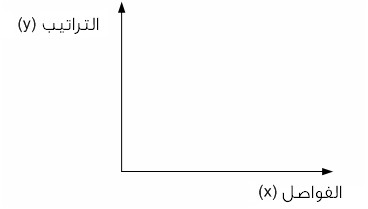
\includegraphics[width=0.4\textwidth]{Chapter_II-6_Axis}
\end{figure}

عندما نعمل في
\textenglish{2D}
لدينا محوران : محور الفواصل (من اليسار إلى اليمين) و محور التراتيب (من الأسفل إلى الأعلى). من العادة أن نرمز للفواصل بمتغيّر يدعى
\InlineCode{x}
و للتراتيب بـ\InlineCode{y}.

هل يمكنك كتابة هيكل
\InlineCode{Coordinates}
يسمح بتخزين كلّا من الفاصلة
(\InlineCode{x})
و الترتيبة
(\InlineCode{y})
لنقطة ما~؟\\
هيّا، هيّا، الأمر ليس صعبا :

\begin{Csource}
struct Coordinates
{
	int x; // Abscissas
	int y; // Ordinates
};
\end{Csource}

هيكلنا يسمّى
\InlineCode{Coordinates}
و هو متكوّن من متغيرين
\InlineCode{x}
و
\InlineCode{y}
أي الفاصلة
(\textenglish{Abscissa})
و الترتيبة
(\textenglish{Ordinate}).

إن أردنا، يمكننا بسهولة إنشاء هيكل
\InlineCode{Coordinates}
من أجل
\textenglish{3D} :
يكفي فقط إضافة متغيّر ثالث (مثلا
\InlineCode{z})
يدلّ على الارتفاع. بهذا سيكون لدينا هيكل لإدارة النقاط الثلاثيّة الأبعاد في الفضاء~!

\subsection{جدول داخل هيكل}

يمكن للهياكل أن تحتوي على جداول. هذا جيّد، إذ يمكننا أن نضع داخلها جداول
\InlineCode{char}،
(سلاسل محرفيّة) بدون أيّة مشاكل.\\
فلنتخيل هيكلاً
\InlineCode{Person}
و الذي يحتوي على معلومات عن شخص :

\begin{Csource}
struct Person
{
	char firstName[100];
	char lastName[100];
	char address[1000];
	int age;
	int boy; // Boolean : 1 = boy, 0 = girl
};
\end{Csource}

هذا الهيكل متشكّل من 5 متغيرات داخليّة، الثلاث الأولى هي سلاسل محرفيّة لتخزين الاسم، اللقب و العنوان.\\
المتغيران الأخيران يخزّنان عُمر و جنس الشخص. الجنس هو متغيّر منطقي، 1 = صحيح = ولد و 0 = خطأ = بنت.

يمكن لهذا الهيكل أن يساعدنا في كتابة برنامج مذكّرة عناوين. يمكنك بالطبع إضافة القدر الذين تريد من المتغيرات داخل الهيكل من أجل إتمامها إذا أردت. لا يوجد حدّ لعدد المتغيّرات في هيكل.

\section{استعمال هيكل}

و الآن، بما أن الهيكل معرّف في ملف
\InlineCode{.h}،
سنتمكّن من استعماله في دالة موجودة بملف
\InlineCode{.c}.\\
أنظر كيف نقوم بإنشاء متغير من نوع
\InlineCode{Coordinates}
(الهيكل الّذي عرّفناه سابقا) :
\begin{Csource}
#include "main.h" // Including the files that contains the prototypes and structures
int main(int argc, char *argv[])
{
	struct Coordinates point; // Creating a variable "point" of type Coordinates
	return 0;
}
\end{Csource}
هكذا نكون قد أنشأنا متغيراً
\InlineCode{point}
من نوع
\InlineCode{Coordinates} !
هذا المتغير سيحمل داخله مركّبين (متغيرين داخليين) :
\InlineCode{x}
و
\InlineCode{y}
(فاصلته و ترتيبته).

\begin{question}
  هل من اللازم أن نضع الكلمة المفتاحية
\InlineCode{struct}
عند تعريف المتغير ؟
\end{question}

نعم، فهذا يسمح للحاسوب بأن يفرّق بين نوع عادي (مثل
\InlineCode{int})
و نوع مخصّص.\\
المبرمجون وجدوا أنه من المتعب جدّا أن يكتبوا في كلّ مرة الكلمة
\InlineCode{struct}
في كلّ تعريف لمتغيّر مخصّص.
لمعالجة هذا المشكل، اخترعوا تعليمة خاصّة : الـ\InlineCode{typedef}.

\subsection{الـ\texttt{typedef}}

لنعد إلى الملف
\InlineCode{.h}
الذي يحمل تعريف هيكلنا من نوع
\InlineCode{Coordinates}.
سنضيف تعليمة اسمها
\InlineCode{typedef}
و الّتي تفيد في إعطاء اسم مستعار
(\textenglish{alias})
لهيكل، أي كتابة شيء مكافئ لكتابة آخر.

إذا، سنضيف سطرا يبدأ بـ\InlineCode{typedef}
قبل تعريف الهيكل مباشرة :

\begin{Csource}
typedef struct Coordinates Coordinates;
struct Coordinates
{
	int x;
	int y;
};
\end{Csource}

هذا السطر متكون من ثلاثة أجزاء :

\begin{itemize}
  \item \InlineCode{typedef} :
  تعني أننا سنقوم بإنشاء اسم مستعار لهيكل.
  \item \InlineCode{struct Coordinates} :
  هو اسم الهيكل الذي سنقوم بانشاء اسم مستعار له (أي "مكافئ").
  \item \InlineCode{Coordinates} :
  هو الاسم المكافئ.
\end{itemize}

ببساطة، هذا السطر يقول : "كتابة
\InlineCode{Coordinates}
مكافئ لكتابة
\InlineCode{struct Coordinates}".
بفعل هذا، لن يكون عليك كتابة الكلمة
\InlineCode{struct}
عند كلّ تعريف لمتغيّر من نوع
\InlineCode{Coordinates}.
يمكننا العودة إلى
\InlineCode{main}
و كتابة فقط :

\begin{Csource}
int main(int argc, char *argv[])
{
	 Coordinates point; // The computer understands that we are talking about "struct Coordinates" thanks to typedef
   return 0;
}
\end{Csource}

أنصحك أن تستعمل الـ\InlineCode{typedef}
مثلما فعلت أنا هنا من أجل
\InlineCode{Coordinates}.
أغلب المبرمجين يفعلون هذا. هذا يسمح لهم بعدم كتابة
\InlineCode{struct}
في كلّ مرّة. المبرمج الجيّد هو مبرمج كسول ! أي أنه يكتب أقل ما يمكن.

\subsection{تغيير مركّبات هيكل}

و الآن بعدما قمنا بإنشاء متغيّرنا
\InlineCode{point}،
نريد أن نغيّر إحداثيّاته.\\
كيف نصل إلى
\InlineCode{x}
و
\InlineCode{y}
الموجودة في المتغير
\InlineCode{point}
؟ هكذا :

\begin{Csource}
int main(int argc, char *argv[])
{
	Coordinates point;
	point.x = 10;
	point.y = 20;
	return 0;
}
\end{Csource}

بهذا نكون قد غيّرنا قيمة
\InlineCode{point}،
بإعطائه الفاصلة 10 و الترتيبة 20. نقطتنا أصبحت في الوضعية (10؛20) (هذا هو الترميز الرياضياتي للإحداثيّات).

لكي نتمكن من الوصول إلى مركّب في الهيكل، يجب كتابة :

\begin{Csource}
  variable.componentName
\end{Csource}

النقطة هي التي تفرّق بين المتغير و المركّب.

إن أخذنا الهيكل
\InlineCode{Person}
الذي رأيناه منذ قليل و نطلب الاسم و اللقب فسنفعل هكذا :

\begin{Csource}
int main(int argc, char *argv[])
{
	Person user;
	printf("What's your last name ? ");
	scanf("%s", user.lastName);
	printf("What's your first name ? ");
	scanf("%s", user.firstName);
	printf("You are %s %s", user.firstName, user.lastName);
	return 0;
}
\end{Csource}

\begin{Console}
What's your last name ? Dupont
What's your first name ? Jean
You are Jean Dupont
\end{Console}

نرسل المتغير
\InlineCode{user.lastName}
إلى الدالة
\InlineCode{scanf}،
و التي ستكتب مباشرة في
\InlineCode{user}.\\
نفعل نفس الشيء مع
\InlineCode{firstName}،
يمكننا فعل ذلك أيضا مع العنوان، العمر و الجنس، لكنّي لا أرغب بتكرار ذلك (يحب أن أكون مبرمجا !).

يمكن فعل هذا بدون معرفة الهياكل، فقط بإنشاء متغيّر
\InlineCode{lastName}
و آخر
\InlineCode{firstName}.\\
لكن الفائدة هنا هي أنه بهذه الطريقة يمكننا أن ننشئ متغيرا آخر من نوع
\InlineCode{Person}
و يكون لديه هو أيضا اسمه الخاص، لقبه الخاص، إلخ. يمكننا إذن فعل هذا :

\begin{Csource}
Person player1, player2;
\end{Csource}

و هكذا نخزّن معلومات كلّ لاعب. كلّ لاعب سيكون لديه اسمه الخاص، لقبه الخاص، إلخ.

يمكننا أن نفعل ما هو أفضل : يمكننا تعريف جدول من
\InlineCode{Person} !\\
القيام بهذا سهل :

\begin{Csource}
Person players[2];
\end{Csource}

و بعدها يمكننا الوصول إلى لقب اللاعب المتواجد بالخانة الأولى مثلا، هكذا :

\begin{Console}
players[0].lastName
\end{Console}

الفائدة من استعمال الجدول هنا، هو أنها بامكاننا استعمال حلقة لنقرأ المعلومات الخاصة باللاعب 1 و اللاعب 2 بدون الاضطرار إلى إعادة الشفرة مرّتين. يكفي تصفّح الجدول
\InlineCode{players}
و طلب كلّ مرّة اللقب، الاسم، العنوان \dots

\paragraph{تمرين :}
قم بتعريف جدول من نوع
\InlineCode{Person}،
و اقرأ المعلومات الخاصة بكلّ لاعب باستخدام حلقة. إبدأ بجدول ذي خانتين، و إن كان ذلك ممتعا، حاول تكبير العدد لاحقا.\\
في النهاية، عليك بإظهار المعلومات التي أخذتها من كلّ لاعب.

\subsection{تهيئة هيكل}

بالنسبة للهياكل، مثل كلّ المتغيرات، الجداول و المؤشّرات، فنحن نفضّل أن نعطيها قيما ابتدائية كي نضمن أنّها لن تحوي "قيما عشوائية". في الواقع، أعيد تذكيرك، المتغير الّذي يتمّ إنشائه يأخذ القيمة الموجودة في الذاكرة حيث تمّ وضعه. أحيانا تكون هذه القيمة $ 0 $، و أحيانا بقايا برنامج مرّ قبلك، لذلك ستكون قيمته شيئا لا معنى له، مثل
$-84570$.

للتذكير، هكذا نقوم بالتهيئة :

\begin{itemize}
  \item  المتغير : نعطيه القيمة 0 (الحالة الأبسط).
  \item المؤشّر : نجعل قيمته
\InlineCode{NULL}.
بالمناسبة فـ\InlineCode{NULL}
هي
\InlineCode{\#define}
موجود في مكتبة
\InlineCode{stdlib.h}
و هي عادة 0، لكنّنا نستمرّ في استخدام
\InlineCode{NULL}
للمؤشرات لكي نبيّن أنّها مؤشّرات و ليست متغيّرات عاديّة.
  \item الجدول : نضع كلّ خاناته على القيمة 0.
\end{itemize}

بالنسبة للهياكل، فالتهيئة شبيهة بتلك الخاصّة بالجدول. في الواقع، يمكننا القيام بها عند التصريح عن المتغيّر :

\begin{Csource}
Coordinates point = {0, 0};
\end{Csource}

و هذا يعرّف بالترتيب :
\InlineCode{point.x = 0}
و
\InlineCode{point.y = 0}.
لنعد إلى الهيكل
\InlineCode{Person}
(الذي يحتوي سلاسل محرفيّة). يمكننا أن نعطي قيمة ابتدائية للسلاسل بكتابة فقط
\InlineCode{""}
(لا شيء ببن علامتي الاقتباس). لم أعلمك هذا الشيء في الفصل الخاصّ بالسلاسل، لكنّ الوقت ليس متأخّرا على تعلّمها.
يمكننا إذن تهيئة على الترتيب
\InlineCode{firstName}،
\InlineCode{lastName}،
\InlineCode{address}،
\InlineCode{age}،
و
\InlineCode{boy}
هكذا :

\begin{Csource}
Person user= {"", "", "", 0, 0};
\end{Csource}

رغم ذلك، أنا لا أستخدم هذه التقنيّة كثيرا. أفضّل أن أرسل متغيّري، مثلا
\InlineCode{point}،
إلى دالّة
\InlineCode{initializeCoordinates}
تقوم بالتهيئات من أجلي على متغيري.\\
لفعل هذا، يجب إرسال مؤشّر نحو متغيري. في الواقع، إن أرسلت فقط المتغيّر، سيتم إنشاء نسخة عنه (مثل أيّ متغيّر عادي) و تعديل قيم النسخة لا قيم المتغيّر. راجع الخيط الأحمر من فصل المؤشرات إن نسيت كيف يعمل هذا الأمر.

يجب إذن تعلّم كيفيّة استخدام المؤشرات على الهياكل. الأمور بدأت تصعب قليلا !

\section{مؤشّر نحو هيكل}

المؤشّر على الهيكل يتمّ إنشائه بنفس طريقة إنشاء مؤشّر على
\InlineCode{int}
أو
\InlineCode{double}
أو أيّ نوع قاعديّ آخر :

\begin{Csource}
Coordinates* point = NULL;
\end{Csource}
بهذا نكون قد عرّفنا مؤشّرا نحو
\InlineCode{Coordinates}
اسمه
\InlineCode{point}.\\
و لأن التذكير لن يضرّ أحدا، أعيد إخبارك بأنه من الممكن وضع النجمة أمام اسم المتغيّر، فهذه الكتابة مكافئة تماما للسابقة~:

\begin{Csource}
Coordinates *point = NULL;
\end{Csource}

أنا أفعل هكذا كثيرا، لأنه لتعريف عدّة مؤشرات على سطر واحد، سيكون علينا وضع النجمة أمام اسم كل واحد منها :

\begin{Csource}
Coordinates *point1 = NULL, *point2 = NULL;
\end{Csource}

\subsection{إرسال هيكل إلى دالة}

الشيء الذي يهمّنا هنا، هو كيفيّة إرسال مؤشر هيكل إلى دالة كي تقوم هذه الأخيرة بتعديل محتواه.

هذا ما سنقوم به في هذا المثال، سنقوم بإنشاء متغير من نوع
\InlineCode{Coordinates}
في
\InlineCode{main}،
و نرسل عنوانه إلى
\InlineCode{initializeCoordinates}.
دور هذه الدالة هو إعطاء القيمة 0 لعناصر الهيكل.

دالتنا
\InlineCode{initializeCoordinates}
ستأخذ معاملا واحدا : مؤشر نحو هيكل من نوع
\InlineCode{Coordinates}
(أي
\InlineCode{*Coordinates}).

\begin{Csource}
int main(int argc, char *argv[])
{
	Coordinates myPoint;
	initializeCoordinates(&myPoint);
	 return 0;
}
void initializeCoordinates(Coordinates* point)
{
	// Initializing each member of the structure here
}
\end{Csource}

متغيري
\InlineCode{myPoint}
تم إنشاؤه في
\InlineCode{main}.\\
نقوم يارسال عنوانه إلى الدالة
\InlineCode{initializeCoordinates}
الّتي تسترجعه على شكل متغيّر يسمّى
\InlineCode{point}
(كان بإمكاننا تسميته كما شئنا، هذا الأمر ليس له أيّ تأثير).

الآن بما أنّنا داخل الدالة
\InlineCode{initializeCoordinates}،
سنقوم يتهيئة قيم المتغير
\InlineCode{point}
واحدة بواحدة.\\
يجب عدم نسيان وضع النجمة أمام اسم المؤشر للوصول إلى المتغير. إن لم تفعل، فأنت تخاطر بتغيير العنوان، و ليس هذا ما نريد فعله.

و لكن هاهي مشكلة \dots لا يمكننا القيام مباشرة بهذا :

\begin{Csource}
void initializeCoordinates(Coordinates* point)
{
	*point.x = 0;
	*point.y = 0;
}
\end{Csource}

سيكون ذلك سهلا جدّا \dots لماذا لا يمكننا القيام بهذا ؟
لأنّ النقطة تطبّق على
\InlineCode{point}
فقط و ليس على
\InlineCode{*point}.
لكنّ ما نريده هو الوصول إلى
\InlineCode{*point}
لتغيير قيمته.\\
لحلّ هذا المشكل، يجب وضع الأقواس حول
\InlineCode{*point}،
هكذا ستطبّق النقطة على
\InlineCode{*point}
و ليس فقط على
\InlineCode{point} :

\begin{Csource}
void initializeCoordinates(Coordinates* point)
{
	(*point).x = 0;
	(*point).y = 0;
}
\end{Csource}

هذه الشفرة تعمل، يمكنك تجريبها. المتغير من نوع
\InlineCode{Coordinates}
تمّ إرساله إلى الدالة التي هيّأت
\InlineCode{x}
و
\InlineCode{y}
على 0.

\begin{information}
في لغة الـ\textenglish{C}،
نهيّئ عادة هياكلنا بالطريقة الّتي رأيناها سابقا. بالمقابل، في لغة الـ\textenglish{C++}،
التهيئة تكون في الغالب داخل "دوال".
إن لغة
\textenglish{C++}
ليست سوى "تحسين خارق" للهياكل. كثير من الأشياء تبدأ من هذا و أحتاج إلى كتاب كامل لأتحدّث عنها (كلّ شيء في وقته).
\end{information}

\subsection{اختصار عمليّ و مستعمل بكثرة}

سترى أننا سنستعمل كثيراً مؤشرات نحو هياكل. بصراحة، يجب أن أعترف لك بأنّه
في لغة الـ\textenglish{C}
نستخدم  المؤشرات نحو الهياكل أكثر من استعمال الهياكل وحدها. لهذا فعندما أقول لك بأنّ المؤشرات ستظلّ تتبعك حتّى إلى قبرك، فأنا لا أقولها تقريبا من أجل المزاح !

بما أن المؤشرات نحو الهياكل مستعملة بكثرة، نجد أنفسنا نستعمل هذه الكتابة كثيرا :
\begin{Csource}
(*point).x = 0;
\end{Csource}

مرّة أخرى، المبرمجون وجدوا هذه الكتابة طويلة جدّا. الأقواس حول
\InlineCode{*point}،
يا لها من بلوى~! إذن، بما أن المبرمجين أشخاص كسالى (لقد قلت هذا سابقا على ما أعتقد)، فقد اخترعوا هذا الاختصار :

\begin{Csource}
point->x = 0;
\end{Csource}

هذا الاختصار يتمّ كتابته بمطّة
\InlineCode{-}
متبوعة بعلامة ترتيب
\InlineCode{>}.

كتابة
\InlineCode{point->x}
هو إذن مكافئ
\underline{تماما}
لكتابة
\InlineCode{(*point).x}.

\begin{warning}
  لا تنس أننا لا نستطيع استعمال السهم إلا مع المؤشرات.\\
إن كنت تعمل على المتغير مباشرة، يجب عليك استخدام النقطة كما رأينا في البداية.
\end{warning}

لنعد إلى دالتنا
\InlineCode{initializeCoordinates}
يمكننا كتابتها بالشكل التالي :

\begin{Csource}
void initializingCoordinates(Coordinates* point)
{
	point->x = 0;
	point->y = 0;
}
\end{Csource}

و تذكّر جيّدا اختصار السهم، سنستعمله كثيراً من الآن. و خاصّة لا تخلط بين السهم و "النقطة". السهم مخصّص للمؤشّرات، "النقطة" مخصّصة للمتغيّرات. استخدم هذا المثال الصغير للتذكّر :

\begin{Csource}
int main(int argc, char *argv[])
{
	Coordinates  myPoint;
	Coordinates *pointer = &myPoint;
	myPoint.x = 10; // We work on a variable, we use the "dot"
	pointer->x = 10; // We work on a pointer, we use the arrow
	return 0;
}
\end{Csource}

نغيّر قيمة
\InlineCode{x}
إلى 10 بطريقتين مختلفتين، هنا : الطريقة الأولى هي بالعمل مباشرة على المتغير، و الطريقة الثانية باستعمال المؤشر.

\section{التعدادات}

التعدادات هي طريقة مختلفة قليلاً لنعرّف نوع متغيرات خاص بنا.

التعداد ليس متكوّنا من "مركّبات"  كما هو الحال مع الهياكل. و إنما هو مجموعة من "القيم الممكنة" لمتغيّر. التعداد سيأخذ إذن خانة واحدة في الذاكرة و هذه الخانة تأخذ قيمة واحدة من مجموع القيم التي قمت بتعريفها (واحدة فقط في كلّ مرّة).
هذا مثال عن تعداد :
\begin{Csource}
typedef enum Volume Volume;
enum Volume
{
	LOW, MEDIUM, HIGH
};
\end{Csource}
تلاحظ أننا نستعمل
\InlineCode{typedef}
هنا أيضا، مثلما رأينا لحد الآن.

لكي نقوم بتعريف تعداد نستعمل الكلمة المفتاحية
\InlineCode{enum}.
اسم التعداد هنا هو
\InlineCode{Volume}.
إنّه نوع مخصّص قمنا بتعريفه يمكن له أن يأخذ واحدة من الثلاث قيم الّتي وضعناها : إما
\InlineCode{LOW}
أو
\InlineCode{MEDIUM}
أو
\InlineCode{HIGH}.

يمكننا إذن أن نعرّف متغيرا اسمه
\InlineCode{music}
من نوع
\InlineCode{Volume}
لتخزين مستوى صوت الموسيقى.\\
يمكننا تهيئة الموسيقى على المستوى
\InlineCode{MEDIUM} :
\begin{Csource}
Volume music = MEDIUM;
\end{Csource}
يمكننا لاحقاً في الشفرة، أن نغيّر قيمة مستوى الصوت و وضعها إمّا على
\InlineCode{HIGH}
أو على
\InlineCode{LOW}.

\subsection{إرفاق قيم التعداد بأعداد}
قد لاحظت أنّي كتبت القيم الممكنة بأحرف كبيرة. هذا يفترض به أن يذكّرك بالثوابت و
\InlineCode{\#define}،
أليس كذلك ؟

في الواقع، إنّ هذا مشابه كثيرا و لكنّه ليس نفس الشيء.\\
المترجم يقوم تلقائيا بارفاق قيم التعداد بأعداد موافقة لها.


في حالة تعدادنا
\InlineCode{Volume}،
\InlineCode{LOW}
سيتم ارفاقها بالقيمة 0،
\InlineCode{MEDIUM}
بالقيمة 1،
و
\InlineCode{HIGH}
بالقيمة 2.\\
الإرفاق يتمّ تلقائيّا انطلاقا من 0.

خلافا لـ\InlineCode{\#define}،
فالمترجم هو من يرفق
\InlineCode{MEDIUM}
بـ1 مثلا، وليس المعالج القبلي. لكنّ هذا سيكون تقريبا مكافئا له.\\
بطبيعة الحال، عندما هيّئنا المتغيّر
\InlineCode{music}
على
\InlineCode{MEDIUM}،
فإنّنا قد وضعنا القيمة 1 في خانة الذاكرة الموافقة.

\begin{question}
عمليّا، هل يهمّنا أن نعرف أنّ
\InlineCode{MEDIUM}
تساوي 1،
\InlineCode{HIGH}
تساوي 2، إلخ. ؟
\end{question}

لا. فهذا حقيقة لا يعنينا. المترجم هو من سيقوم تلقائيّا بإرفاق العدد المناسب إلى كلّ قيمة. بفضل هذا، ليس عليك سوى كتابة :
\begin{Csource}
if (music == MEDIUM)
{
	// Play music with medium volume
}
\end{Csource}
لا يهمّ ما هي قيمة
\InlineCode{MEDIUM}،
ستترك المترجم يهتمّ بالأعداد.

الفائدة من كلّ  هذا ؟  هي أنها تجعل الشفرة قابلة للقراءة جيّدا. في الواقع، أيّ شخص يمكنه بسهولة قراءة
\InlineCode{if}
السابق (نفهم جيّدا أنّ الشرط يعني "إن كانت الموسيقى بمستوى صوت متوسّط").

\subsection{ارفاق قيمة محددة}
حاليّا، كان المترجم هو من يقرّر إرفاق العدد 0 ثم 1، 2، 3
 بالترتيب.\\
من الممكن طلب إرفاق قيمة محدّدة لكلّ عنصر من التعداد.

ما الفائدة التي يمكن تحصيلها من هذا ؟ حسنا فلنفرض أنّه في حاسوبك، الصوت يتم تحديده بقيمة بين 0 و 100 (0 = لا صوت، 100 = 100\%
من الصوت)، فسيكون من الجيد ارفاق قيمة محدّدة بكلّ عنصر :
\begin{Csource}
typedef enum Volume Volume;
enum Volume
{
	LOW = 10, MEDIUM = 50, HIGH = 100
};
\end{Csource}
هنا، المستوى
\InlineCode{LOW}
يوافق 10\%
من المستوى، المستوى
\InlineCode{MEDIUM}
يوافق 50\%،
إلخ.\\
يمكننا بسهولة إضافة بعض القيم الأخرى مثل
\InlineCode{MUTE}.
نرفق في هذه الحالة
\InlineCode{MUTE}
بالقيمة \dots 0 ! لقد فهمت.

\section*{ملخّص}

\begin{itemize}
  \item الهيكل هو نوع بيانات مخصّص يمكنك إنشاؤه و استخدامه في برامجك. يجب عليك تعريفه، عكس الأنواع القاعديّة مثل
\InlineCode{int}
و
\InlineCode{double}
الّتي نجدها في كلّ البرامج.
  \item الهيكل يتكوّن من "متغيّرات داخليّة" تكون عادة من أنواع قاعديّة مثل
\InlineCode{int}
و
\InlineCode{double}،
و أيضا من الجداول.
  \item نستطيع الوصول إلى أحد مركّبات الهيكل بفصل اسم المتغيّر و المركّب بنقطة :
\InlineCode{player.firstName}.
  \item إذا كنّا نتعامل مع مؤشر نحو هيكل و أردنا الوصول إلى أحد مركّباته، نستخدم السهم بدل النقطة :\\
\InlineCode{playerPointer->firstName}.
  \item التعداد هو نوع مخصّص يمكنه فقط أخذ إحدى القيم المسبقة التعريف :
\InlineCode{LOW}،
\InlineCode{MEDIUM}
أو
\InlineCode{HIGH}
مثلا.
\end{itemize}

  \chapter{قراءة و كتابة الملفات}
المشكل مع استعمال المتغيّرات، هو أنها موجودة فقط في الذاكرة العشوائية
\textenglish{RAM}.
بخروجنا من البرنامج، كلّ المتغيّرات يتم حذفها من الذاكرة و لن يصبح ممكنا إستعادة قيمها. كيف يمكننا إذن أن نحتفظ بأحسن العلامات التي تحصّلنا عليها في لعبة ؟ كيف يمكننا إنشاء محرر نصوص إذا كان كلّ النصّ  المكتوب يختفي بمجرّد إيقاف البرنامج ؟

لحسن الحظّ يمكننا القراءة من الملفاّت و كذا الكتابة فيها في لغة
\textenglish{C}.
هذه الملفّات مُخزّنة في القرص الصلب
(\textenglish{Hard disk})
الخاص بالحاسوب : الشيء الإيجابيّ إذن هو أنها تبقى محفوظة، حتّى عند إيقاف البرنامج أو الحاسوب.

للقراءة من الملفات و الكتابة فيها، سنحتاج إلى استعمال كلّ ما درسناه حتّى الآن : المؤشرات، الهياكل، السلاسل المحرفيّة، الخ.

\section{فتح و غلق ملف}
للقراءة و الكتابة في الملفّات، سنستعمل دوالاً معرّفة في المكتبة
\InlineCode{stdio}
التي استعملناها سابقاً.\\
نعم، هذه المكتبة تحتوي على الدالتين
\InlineCode{scanf}
و
\InlineCode{printf}
اللتان نعرفهما جيّدا ! لكن ليس هذا فحسب : يوجد بها الكثير من الدوال الأخرى، خصوصا التي تعمل على الملفات.

\begin{information}
  كل المكتبات التي استعملناها حتّى الآن
(\InlineCode{stdlib.h}، \InlineCode{stdio.h}، \InlineCode{math.h}، \InlineCode{string.h}...)
تشكّل ما نسميه بالمكتبات القياسية
(\textenglish{standard libraries})،
و هي مكتبات تأتي تلقائيا مع البيئة التطويرية التي تستخدمها و لديها الميزة في أنّها تعمل على كل أنظمة التشغيل. بالإمكان استعمالها في أيّ مكان، سواء كنت في
\textenglish{Windows}،
أو
\textenglish{GNU/Linux}
أو
\textenglish{Mac}
أو غير ذلك.
المكتبات القياسيّة ليست كثيرة و لا تمكّننا من القيام بأكثر من بعض الأمور الأساسيّة، كما فعلنا لغاية الآن. للحصول على وظائف أكثر تقدّما، كفتح النوافذ، يجب تحميل و تثبيت مكتبات جديدة. سنرى ذلك قريبا !
\end{information}

تأكّد إذن، للبدأ، أن تقوم بتضمين المكتبتين
\InlineCode{stdio.h}
و
\InlineCode{stdlib.h}
على الأقل أعلى ملفكم
\InlineCode{.c} :

\begin{Csource}
#include <stdlib.h>
#include <stdio.h>
\end{Csource}

هاتان المكتبتان ضروريتان و أساسيّتان لدرجة أنّي أنصحك بتضمينهما في كلّ البرامج التي تكتبها في المستقبل، أيّا كانت.

حسناً و بعدما قمنا بتضمين المكتبتين، يمكننا أن ننطلق في بالأمور الجدّيّة. إليك الخطوات التي يجب إتّباعها دائماً حينما تريد العمل على ملف، سواء للقراءة منه أو للكتابة فيه :
\begin{itemize}
  \item نقوم بمناداة دالة
\textbf{فتح الملف}
\InlineCode{fopen}
التي تقوم بإرجاع مؤشّر نحو هذا الملف.
  \item \textbf{نتأكّد من نجاح عمليّة الفتح}
(أي إن كان الملفّ موجودا) باختبار قيمة المؤشر الذي أرجعته الدالة. فإن كان المؤشر يساوي
\InlineCode{NULL}،
فهذا يعني أنّ فتح الملف لم ينجح، في هذه الحالة لا يمكننا الإكمال (يجب أن نظهر رسالة خطا).
  \item إذا تم الفتح بنجاح (أي أن قيمة المؤشر تختلف عن
\InlineCode{NULL})،
سنستمتع
\textbf{بالكتابة على الملف أو القراءة منه}،
و ذلك باستخدام دوال سنراها لاحقاً.
  \item بمجرّد أن
\textbf{ننهي العمل على الملف}،
يجب تذكّر "غلقه" باستعمال الدالة
\InlineCode{fclose}.
\end{itemize}
سنتعلّم كخطوة أولى كيف نستخدم
\InlineCode{fopen}
و
\InlineCode{fclose}،
حينما تتعلّم هذا، سنتعلّم كيف نقرأ محتواه و نكتب نصّا فيه.

\subsection{\texttt{fopen} : فتح ملف}
في فصل السلاسل المحرفيّة، كنا نستعين بنماذج الدوال مثل "دليل استخدام". هذا ما يفعله المبرمجون غالبا : يقرؤون نموذج دالة و يفهمون كيف يستخدمونها. مع ذلك، أعلم أنّنا بحاجة إلى بعض الشروحات البسيطة !

لهذا فلنرى قليلاً نموذج
\InlineCode{fopen} :

\begin{Csource}
FILE* fopen(const char* fileName, const char* openMode);
\end{Csource}

هذه الدالة تنتظر معاملين :
\begin{itemize}
  \item اسم الملف الذي نريد فتحه.
  \item أسلوب فتح الملف، أي دلالة تذكر ما الّذي تريد فعله : القراءة من الملف، أو الكتابة فيه، أو كليهما.
\end{itemize}

هذه الدالة ترجع... مؤشّرا على
\InlineCode{FILE} !
إنّه مؤشّر على هيكل من نوع
\InlineCode{FILE}.
هذا الهيكل متواجد في المكتبة
\InlineCode{stdio.h}.
يمكنك فتح الملف لترى مما يتكوّن النوع
\InlineCode{FILE}،
لكن هذا ليس ما يهمّنا.

\begin{question}
  لكن لِمَ اسم الهيكل كله بأحرف كبيرة؟ اعتقدت أن الأسماء بالأحرف الكبيرة حجزناها للثوابت و لـ\InlineCode{\#define} ؟
\end{question}

هذه "القاعدة"، أنا من قمت بتحديدها (و كثير من المبرمجين يتيعونها)، و لكنّها لم تكن أبدا مفروضة. و يبدو أنّ من برمجوا
\InlineCode{stdio.h}
لا يتبعون نفس القواعد !\\
هذا لا يجب أن يشوّشك كثيرا. سوف ترى أنّ المكتبات الّتي سندرسها لاحقا تتبّع نفس القواعد التي أتّبعها، أي أن اسم الهيكل يبتدئ فقط بحرف واحد كبير.

لنعد إلى دالتنا
\InlineCode{fopen}،
إنها تقوم بارجاع
\InlineCode{FILE*}.
إنه من المهم جدّا استرجاع هذا المؤشّر كي نتمكّن لاحقاً من القراءة و الكتابة في الملف.  و لهذا سنقوم بإنشاء مؤشّر على
\InlineCode{FILE}،
في بداية دالتنا
(\InlineCode{main}
مثلا) :

\begin{Csource}
int main(int argc, char *argv[])
{
	FILE* file = NULL;
	return 0;
}
\end{Csource}

لقد هيّأنا المؤشّر على
\InlineCode{NULL}
من البداية. أذكّرك بأنّ هذه قاعدة أساسيّة أن تهيّأ كلّ المؤشّرات على
\InlineCode{NULL}
إنّ لم تكن لديك قيمة أخرى لإعطائها. إن لم تفعل ذلك، فأنت تزيد كثيرا خطر وجود أخطاء لاحقا.

\begin{information}
  إنه ليس ضرورياً أن تكتب
\InlineCode{struct FILE* file = NULL}،
لأن منشئي
\InlineCode{stdio.h}
قد وضعوا
\InlineCode{typedef}
كما علّمتك منذ مدّة قصيرة.
لاحظ أن شكل الهيكل قد يتغيّر من نظام تشغيل إلى آخر (لا تملك بالضرورة نفس المركّبات في كل الأنظمة). لهذا فلن نعدّل محتوى
\InlineCode{FILE}
مباشرة (لا نقوم بـ\InlineCode{file.element}
مثلا). بل سنكتفي باستدعاء دوال، تتعامل مع
\InlineCode{FILE}
نيابة عناً.
\end{information}

الآن سنقوم بمناداة الدالة
\InlineCode{fopen}،
و استرجاع القيمة الّتي تعيدها في المؤشر
\InlineCode{file}.
و لكن قبل هذا يجب أن اشرح لك كيف تستخدم المعامل الثاني
\InlineCode{openMode}.
في الواقع، هناك شفرة تدلّ للحاسوب على أنك تريد أن تفتح الملف بوضع القراءة فقط، الكتابة فقط أو الاثنين معاً.\\
هذه هي أوضاع فتح الملف المختلفة :
\begin{itemize}
  \item \textbf{\textenglish{"r"} :
قراءة فقط
(\textenglish{read only})}.
يمكنك قراءة محتوى الملف، و لكن لا يمكنك الكتابة فيه.
\textit{يجب أن يكون الملف موجوداً من قبل}.
  \item \textbf{\textenglish{"w"} :
كتابة فقط
(\textenglish{write only})}.
يمكنك الكتابة في الملف، لكن لا يمكنك قراءة محتواه.
\textit{إذا لم يكن الملف موجوداً من قبل، فإنه سيتم إنشاؤه}.
  \item \textbf{\textenglish{"a"} :
إلحاق
(\textenglish{append})}.
يمكنك الكتابة في الملف، إنطلاقا من نهايته.
\textit{إن لم يكن الملف موجوداً، فسيتم إنشاؤه}.
  \item \textbf{\textenglish{"r+"} :
قراءة و كتابة
(\textenglish{read and write})}.
يمكنك القراءة من الملف و الكتابة فيه.
\textit{يجب أن يكون الملف موجوداً من قبل}.
  \item \textbf{\textenglish{"w+"} :
قراءة و كتابة مع مسح المحتوى أوّلا}.
سيتم تفريغ الملف من محتواه أولاً، ثم بإمكانك الكتابة فيه و قراءة محتواه بعد ذلك.
\textit{إن لم يكن الملف موجوداً من قبل، سيتم إنشاؤه}.
  \item \textbf{\textenglish{"a+"}
إلحاق مع القراءة / الكتابة في آخر الملف}.
يمكنك القراءة و الكتابة إنطلاقا من نهاية الملف.
\textit{إن لم يكن موجوداً، سيتم إنشاؤه}.
\end{itemize}

لمعلوماتك، أنا عرضت لك بعضا من أوضاع فتح ملف. في الحقيقة، يوجد ضعفها !
من أجل كل وضع رأيناه هنا، إن أضفت
\InlineCode{"b"}
بعد المحرف الأول
(\InlineCode{"rb"}، \InlineCode{"wb"}، \InlineCode{"ab"}، \InlineCode{"rb+"}، \InlineCode{"wb+"}، \InlineCode{"ab+"})،
فإن الملف سيتم فتحه بالوضع الثنائي
(\textenglish{binary}).
هذا وضع خاص قليلاً فلن ندرسه هنا. في الواقع وضع النص يختصّ بتخزين... النص، تماما كما يوحي الاسم (فقط المحارف القابلة للعرض). أما الوضع الثنائي، يسمح بتخزين المعلومات
بايتا بايتا
(\textenglish{Byte by byte})
(أرقام بشكل أساسي). هذا مختلف كثيرا. على أي حال فطريقة العمل هي تقريبا نفس الّتي سنراها هنا.

شخصياً، أستعمل كثيراً الأوضاع :
\InlineCode{"r"}
(قراءة)،
\InlineCode{"w"}
(كتابة)،
\InlineCode{"r+"}
(قراءة و كتابة في آن واحد). وضع
\InlineCode{"w+"}
خطر قليلاً لأنه يقوم بمسح محتوى الملف مباشرة، بدون أن يطلب التأكيد قبل القيام بذلك. إن هذا الوضع ليس مفيداً إلا إذا أردنا أن نعيد تهيئة الملف أوّلا.
وضع الإلحاق
(\InlineCode{"a"})
يمكنه أن يفيد في بعض الحالات، إذا كنت تريد إضافة معلومات إلى نهاية الملف.

\begin{information}
  إن كنت تريد قراءة ملفّ، فمن المستحسن وضع
\InlineCode{"r"}.
بالطبع، الوضع
\InlineCode{"r+"}
يعمل أيضا، لكن بوضع
\InlineCode{"r"}
فأنت تضمن أنّ الملفّ لا يمكن تعديله، هذا نوع من الحماية.
\end{information}

إن كتبت دالةً
\InlineCode{loadLevel}
(لتحميل مستوى في لعبة مثلا)، الوضع
\InlineCode{"r"}
كافٍ، أما إن أردت أن كتابة دالةٍ
\InlineCode{saveLevel}
(لحفظ المستوى) فستستعمل الوضع
\InlineCode{"w"}.

الشفرة التالية ستفتح الملف
\InlineCode{test.txt}
في وضع
\InlineCode{"r+"}
(قراءة و كتابة) :

\begin{Csource}
int main(int argc, char *argv[])
{
	FILE* file = NULL;
	file = fopen("test.txt", "r+");
	return 0;
}
\end{Csource}

المؤشّر
\InlineCode{file}
يصبح إذن مؤشراً على الملف
\InlineCode{test.txt}.

\begin{question}
  أين يجب أن يكون الملف
\InlineCode{test.txt}
؟
\end{question}

يجب أن يكون في نفس المجلّد الذي يتواجد به الملف التنفيذي
(\InlineCode{.exe}).\\
من أجل متطلّبات هذا الفصل، أطلب منك أن تقوم بإنشاء ملف
\InlineCode{test.txt}
في نفس المساؤ الذي به
\InlineCode{.exe}،
مثلما أفعل أنا (الشكل الموالي).

\Picture{Chapter_II-7_Files}

كما ترى فأنا أستعمل  حاليّا بيئة التطوير
\textenglish{Code::Blocks}
الأمر الذي يفسّر وجود ملف المشروع بصيغة
\InlineCode{.cbp}
(في مكان الصيغة
\InlineCode{.sln}
إن كنت تستعمل
\InlineCode{Visual C++}
مثلاً). باختصار، الأمر المهم هو أن برنامجي
(\InlineCode{tests.exe})
موجود في نفس مجلّد الملف الذي نريد قرائته أو كتابته
(\InlineCode{test.txt}).

\begin{question}
  هل يجب أن يكون الملف بصيغة
\InlineCode{.txt} ؟
\end{question}

لا، الأمر يعود إليك في اختيار صيغة الملف عندما تفتحه. أي أنه بإمكانك أن تخترع صيغتك الخاصّة
\InlineCode{.level}
لحفظ مستويات ألعابك مثلاً.

\begin{question}
  هل من الواجب أن يكون الملف الذي نريد فتحه في نفس دليل الملف التنفيذي ؟
\end{question}

لا أيضا. يمكنه أن يكون داخل مجلّد بذات الدليل :

\begin{Csource}
  file = fopen("directory/test.txt", "r+");
\end{Csource}

هنا، الملف
\InlineCode{test.txt}
في مجلّد  داخليّ اسمه
\InlineCode{directory}.
هذه الطريقة التي نسميها
\textit{المسار النسبي}
عمليّة أكثر. هكذا، يمكن للبرنامج أن يعمل أينما كان مثبّتا.

من الممكن أيضا فتح ملفّ أينما كان في القرص الصلب. في هذه الحالة يجب كتابة المسار الكامل (ما نسميه
\textit{المسار المطلق}) :

\begin{Csource}
  file = fopen("C:\\Program Files\\Notepad++\\readme.txt", "r+");
\end{Csource}

هذه الشفرة تفتح الملف
\InlineCode{readme.txt}
الموجود بـ\InlineCode{C:\textbackslash Program Files\textbackslash Notepad++}.

\begin{warning}
  تعمّدت استعمال شرطتبن خلفيّتين
\InlineCode{\textbackslash}
  كما تلاحظ. في الواقع، إن كتبت اشارة واحدة، سيعتقد الحاسوب أنني أريد أن استخدم رمزا خاصا (مثل الـ\InlineCode{\textbackslash n}
أو الـ\InlineCode{\textbackslash t}).
لكتابة شرطة خلفيّة في سلسلة، يجب كتابتها إذن مرّتين ! هكذا يمكن أن يفهم أنّك تريد استخدام الرمز
\InlineCode{\textbackslash}.
\end{warning}

المشكل مع المسارات المطلقة، هو أنها لا تعمل إلا مع نظام معيّن، فهي ليست حلّا محمولا إذن. أي أنه لو كنت تعمل على
\textenglish{GNU/Linux}
لكان عليك كتابة مسار كهذا مثلا :

\begin{Csource}
  file = fopen("/home/mateo/directory/readme.txt", "r+");
\end{Csource}

لهذا فأنا أنصحك بكتابة مسارات نسبية. لا تستعمل المسارات المطلقة إلا في حالة كان البرنامج مخصص لنظام تشغيل معيّن، ليعدّل على ملف معيّن في القرص الصلب.

\subsection{اختبار فتح ملف}
المؤشّر
\InlineCode{file}
يجب أن يحوي عنوان الهيكل من نوع
\InlineCode{FILE}،
و الذي نستعمله كواصف
(\textenglish{descriptor})
للملف. هذا الواصف تم تحميله من أجلك في الذاكرة من طرف الدالة
\InlineCode{fopen}.
بعد هذا، هناك احتمالان :

\begin{itemize}
  \item إمّا أن تنجح عملية الفتح، فسنتمكن من المواصلة (أي البدء في القراءة و الكتابة في الملف).
  \item إمّا ألّا تنجح لأن الملف ليس موجوداً أو أنه مستخدم من طرف برنامج آخر. في هذه الحالة، سنتوقف عن العمل على الملف.
\end{itemize}

مباشرة بعد فتح الملف، يجب التأكد ما إن تمت العملية بنجاح، أم لا. هذا أمر بسيط : إذا كانت قيمة المؤشر تساوي
\InlineCode{NULL}،
فإن الفتح قد فشل. إن كانت قيمته تساوي شيئا غير
\InlineCode{NULL}،
فقد تم الفتح بنجاح.\\
سنتبع إذن هذا المخطط التالي :

\begin{Csource}
int main(int argc, char *argv[])
{
	FILE* file = NULL;
	file = fopen("test.txt", "r+");
	if (file != NULL)
	{
    		// We can read or write in the file
	}
	else
	{
    		// We display an error message if we want
    		printf("Can't open the file test.txt");
	}
	return 0;
}
\end{Csource}

إفعل هذا دائما عند فتح أي ملف. إن لم تفعل و الملف غير موجود، فأنت تخاطر بتوقّف البرنامج بعدها.

  \chapter{الحجز الحيّ للذاكرة
(\textenglish{Dynamic memory allocation})}

كل المتغيّرات التي أنشأناها لحد الآن تمّ إنشاؤها تلقائيّا من طرف المترجم الخاصّ بلغة
\textenglish{C}.
لقد كانت الطريقة البسيطة. رغم ذلك، توجد طريقة يدوية أكثر لإنشاء متغيّرات و نسمّيها بالحجز الحيّ
(\textenglish{Dynamic allocation}).

من بين فوائد الحجز الحيّ هو السماح لبرنامج بحجز مكان لازم لتخزين جدول في الذاكرة لا يُعرف حجمه قبل بداية الترجمة. في الواقع، حتّى الآن، كان حجم جداولنا ثابتاً في الشفرة المصدريّة. بعد قراءة هذا الفصل، ستستطيع إنشاء جداول بطريقة أكثر مرونة !

من الضروري أن تتقن التعامل مع المؤشرات لتتمكّن من قراءة هذا الفصل ! إن كانت لديك بعض الشكوك حول المؤشرات، أنصحك بالذهاب لإعادة قراءة الفصل الموافق قبل البدأ.

عندما نقوم بالتصريح عن متغيّر، فإننا نقول أننا
\textbf{طلبنا حجز مكان في الذاكرة} :

\begin{Csource}
int myNumber = 0;
\end{Csource}

عندما يصل المترجم إلى سطر مشابه للسطر السابق، يقوم بالأمور التالية :
\begin{itemize}
  \item يقوم البرنامج بطلب إذن من نظام التشغيل
(\textenglish{Windows}، \textenglish{GNU/Linux}، \textenglish{Mac OS}...)
ليحجز شيئا من الذاكرة.
  \item يستجيب نظام التشغيل بإعطاء البرنامج عنوان الخانة حيث يمكنه تخزين المتغيّر (يعطيه العنوان الّذي حجزه له).
  \item عندما تنتهي الدالّة، المتغيّر يتم حذفه من الذاكرة. برنامجك يقول لنظام التشغيل : "أنا لم أعد بحاجة إلى المكان في الذاكرة الّذي حجزته في ذلك العنوان، شكرا ! التاريخ لا يحدّد إن كان البرنامج قد قال فعلا "شكرا" لنظام التشغيل، لكنّ هذا في مصلحته لأنّ نظام التشغيل هو الّذي يتحكم في الذاكرة !
\end{itemize}

لحد الآن كل الأمور كانت تلقائيّة. عندما نصرّح عن متغير فإن نظام التشغيل يتمّ استدعاءه تلقائياً من طرف البرنامج.
ما رأيك إذا بفعل هذا بطريقة يدوية ؟ ليس لأننا نريد أن نستمتع بفعل شيء معقّد، بل لأننا أحيانا نظطرّ لفعل ذلك !

في هذا الفصل سنقوم بـ :
\begin{itemize}
  \item دراسة كيف تعمل الذاكرة (نعم، مرّة أخرى !) لنعرف ما الحجم الذي يحجزه كل متغيّر حسب نوعه.
  \item ثمّ ندخل في موضوعنا الأساسي : سنرى كيف نطلب من نظام التشغيل يدويّا أن يحجز لنا مكانا في الذاكرة. هذا ما سنسميه الحجز الحيّ للذاكرة.
  \item و أخيراً، سنكتشف الفائدة من القيام بالحجز الحيّ بتعلّم إنشاء جدول ذو حجم غير معروف إلّا عند اشتغال البرنامج.
\end{itemize}

\section{حجم المتغيرات}
بحسب نوع المتغير التي نريد إنشاءه
(\InlineCode{int}،
\InlineCode{char}،
\InlineCode{float}...)
فنحن نحتاج إلى حجم معيّن من الذاكرة.

في الواقع، لتخزين عدد من
$-128$
إلى
$127$
(\InlineCode{char})
لن نحتاج إلا إلى بايت واحد من الذاكرة. هذا حجم صغير للغاية.\\
بالمقابل،
\InlineCode{int}
يحجز عادة حوالي 4 بايتات من الذاكرة. بينما
\InlineCode{double}
يحجز 8 بايتات.

المشكل هو ... أن هذا ليس دائما صحيحا. هذا يعتمد على الأجهزة : فقد يكون
\InlineCode{int}
يحجز 8 بايتات. من يعلم ؟\\
هدفنا هنا أن نتعرّف كم يحجز كلّ نوع من حجم في الذاكرة على حاسوبك.

توجد وسيلة سهلة جدّا لمعرفة هذا : استعمال العامل
\InlineCode{sizeof()}.\\
على عكس الظاهر، فهو ليس دالة، بل عبارة عن إحدى الوظائف الأساسية من لغة الـ\textenglish{C}،
يجب عليك فقط أن تضع بين القوسين النوع الذي تريد تحليله.\\
لمعرفة حجم
\InlineCode{int}،
يجب كتابة التالي :

\begin{Csource}
sizeof(int)
\end{Csource}

عند الترجمة، سيتم استبدال هذه الشفرة بعدد : عدد البايتات الّتي يحجزها
\InlineCode{int}
في الذاكرة. بالنسبة لي،
\InlineCode{sizeof(int)}
تساوي 4، و هذا يعني أنّ
\InlineCode{int}
يأخذ 4 بايتات. بالنسبة لك، ستكون نفس القيمة على الأرجح، لكنّها ليست قاعدة. جرّب لترى، بعرض القيمة عن طريق
\InlineCode{printf}
مثلا :

\begin{Csource}
printf("char : %d bytes\n", sizeof(char));
printf("int : %d bytes\n", sizeof(int));
printf("long : %d bytes\n", sizeof(long));
printf("double : %d bytes\n", sizeof(double))
\end{Csource}

بالنسبة لي ، هذا يظهر على الشاشة :

\begin{Csource}
char : 1 bytes
int : 4 bytes
long : 4 bytes
double : 8 bytes
\end{Csource}

لم أختبر كل الأنواع الّتي نعرفها، أتركك لتجرّب أحجام الأنواع الأخرى.

أنت تلاحظ أن
\InlineCode{int}
و
\InlineCode{long}
يحجزان نفس الحجم من الذاكرة. إنشاء
\InlineCode{long}
يعود تماما إلى إنشاء
\InlineCode{int}،
هذا يأخذ 4 بايتات من الذاكرة.

\begin{information}
في الواقع، النوع
\InlineCode{long}
هو مكافئ لنوع نسميه
\InlineCode{long int}،
و الذي هو مكافئ لنوع...
\InlineCode{int}
نفسه. باختصار، فإن هذه أسماء كثيرة مختلفة لأجل أشياء ليست بالكبيرة، في النهاية ! امتلاك أنواع مختلفة كثيرة كان أمرا مهمّا  في الوقت الذي لمّ تكن الحواسيب تملك كثيرا من ذاكرة. كنا نبحث دائما لاستخدام الحدّ الأدنى من الذاكرة باستخدام النوع المناسب.\\
اليوم، هذا لم يعد مفيدا كثيرا لأنّ ذاكرة الحاسوب صارت كبيرة جدّا. بالمقابل، هذه الأنواع لا تزال مفيدة إذا كنت تنشئ برامج للأنظمة المضمّنة
(\textenglish{Embedded systems})
حيث الذاكرة المتوفّرة أقل. أظن مثلا في البرامج الموجّهة للهواتف المحمولة، الأليّات، إلخ.
\end{information}

\begin{question}
هل بإمكاننا أن نُظهر حجم نوع مخصّص قمنا نحن بإنشائه (هيكل) ؟
\end{question}

نعم !
\InlineCode{sizeof()}
تعمل مع الهياكل أيضا !

\begin{Csource}
typedef struct ِCoordinates ِCoordinates ;
struct ِCoordinates
{
	int x;
	int y;
};
int main(int argc, char *argv[])
{
	printf("ِCoordinates  : %d bytes\n", sizeof(ِCoordinates));
	return 0;
}
\end{Csource}

\begin{Console}
Coordinates : 8 bytes
\end{Console}

كلما احتوى الهيكل من مركّبات كلّما أخذ حجما أكثر من الذاكرة. الأمر منطقي تماما، أليس كذلك ؟

\subsection{طريقة أخرى للنظر إلى الذاكرة}
لحد الآن، كل المخططات التي قدّمتها لك عن الذاكرة لم تكن دقيقة. سنجعلها أخيرا دقيقة حقا و صحيحة بما أننا تعلّمنا الآن كم يأخذ كل نوع من حجم بالذاكرة.

إن صرّحنا عن متغير من نوع
\InlineCode{int} :

\begin{Csource}
int number = 18;
\end{Csource}

و
\InlineCode{sizeof(int)}
يعطينا 4 بايت على حاسوبنا، هذا يعني أن المتغير يحجز 4 بايت في الذاكرة !

لنفترض أن المتغير
\InlineCode{number}
محجوز بالعنوان
$1600$
من الذاكرة. سيكون لدينا إذا المخطط التالي للذاكرة :

\Picture{Chapter_II-8_RAM-Schema-int}

هنا، يمكننا فعلاً أن نرى بأن المتغير
\InlineCode{number}
من النوع
\InlineCode{int}
يحجز 4 بايت من الذاكرة.
فهو يبدأ من العنوان
$1600$
و ينتهي عند العنوان
$1603$،
المتغير القادم لن يتم تخزينه إلا إبتداءً من العنوان
$1604$ !

إن جربنا نفس الشيء مع
\InlineCode{char}،
فالمتغير لن يأخذ سوى بايت واحد في الذاكرة (الشكل التالي) :

\Picture{Chapter_II-8_RAM-Schema-char}

تخيّل الآن جدولا من
\InlineCode{int} !\\
كل "خانة" من الجدول ستحجز 4 بايت. إن كان الجدول يحوي مثلاً  100 خانة :

\begin{Csource}
int table[100];
\end{Csource}

سنحجز إذن
$100 * 4 = 400$
بايت في الذاكرة.

\begin{question}
ماذا لو كان الجدول فارغاً، هل سيحجز 400 بايت ؟
\end{question}

نعم بالطبع ! فالمكان  في الذاكرة قد تمّ حجزه، و لا يملك أي برنامج الحقّ في استخدام هذه الخانات (غير هذا البرنامج). بمجرّد التصريح عن متغيّر، سيأخذ مكانه مباشرة المكان في الذاكرة.

لاحظ لو أننا ننشئ جدولا من نوع
\InlineCode{Coordinates} :

\begin{Csource}
Coordinates table[100];
\end{Csource}

سيستخدم هذه المرّة
$8 * 100 = 800$
بايت.

من المهمّ الفهم الجيّد لهذه الحسابات البسيطة لنواصل بقيّة الفصل.

\section{الحجز الحيّ للذاكرة}
فلندخل إلى صلب الموضوع. سأذكّرك بهدفنا : تعلّم كيفيّة طلب الذاكرة يدوياً.

سنحتاج إلى تضمين المكتبة
\InlineCode{stdlib.h}.
إن كنت قد اتّبعت نصائحي، فقد ضمّنتها في كلّ برامجك. هذه المكتبة تحتوي على دالّتين سنحتاج إليهما :
\begin{itemize}
  \item \InlineCode{malloc} ("\textenglish{Memory ALLOcation}"
بمعنى "حجز الذاكرة") : تطلب الإذن من نظام التشغيل لاستخدام الذاكرة.
  \item \InlineCode{free}
(تحرير) : تسمح للإشارة لنظام التشغيل بأننا لم نعد بحاجة إلى الذاكرة الّتي طلبناها. المكان في الذاكرة تمّ تحريره، يستطيع برنامج آخر الآن استخدامها عند الحاجة.
\end{itemize}

عندما تقوم بحجز يدوي للذاكرة، فعليك اتباع الخطوات التالية :
\begin{enumerate}
  \item استدعاء
\InlineCode{malloc}
من أجل طلب الذاكرة.
  \item اختبار القيمة التي تم ارجاعها من طرف
\InlineCode{malloc}
لمعرفة ما إن نجح نظام التشغيل في حجز الذاكرة.
  \item ما إن ننتهي من استخدام الذاكرة، يجب علينا تحريرها باستعمال
\InlineCode{free}.
إن لم نفعل هذا، فسنتعرّض لتسريبات ذاكرة، أي أنّ البرنامج يخاطر بحجز كثير من الذاكرة مع أنّه ليس بحاجة إلى كلّ هذا المكان.
\end{enumerate}

هل تذكّرك هذه الخطوات الثلاث بفصل الملفات ؟ نعم يجب أن تفعل ! المبدأ واحد تماما : نحجز، نختبر إن نجح الحجز، ثمّ نحرر عندما ننتهي من الاستعمال.

\subsection{\texttt{malloc}
لنطلب الإذن لحجز الذاكرة}
نموذج الدالة
\InlineCode{malloc}
هزليّ جدّا، سترى :

\begin{Csource}
void* malloc(size_t numberOfNecessaryBytes);
\end{Csource}

الدالة تأخذ معاملا واحدا : عدد البايتات الّتي يجب حجزها. هكذا، يكفي أن كتابة
\InlineCode{sizeof(int)}
لحجز مكان من أجل تخزين
\InlineCode{int}.

و لكنّ الشيء الذي يثير الفضول، هو القيمة التي ترجعها الدالة : إنّها تعيد ...
\InlineCode{void*} !
إذا لازلت تتذكّر فصل الدوال، كنت قد قلت لك بأن الكلمة
\InlineCode{void}
تعني "الفراغ" و نستعملها لنشير إلى أن الدالة لا تُعيد أية قيمة.

إذن هنا، لدينا دالة تُعيد ... "مؤشّراً نحو فراغ" ؟ هذه نكتة جيدة !\\
يبدو أن هؤلاء المبرمجين لديهم حسّ فكاهي متطوّر.

كن متأكّدا، يوجد سبب. في الحقيقة، هذه الدالة تعيد عنوان الخانة التي حجزها نظام التشغيل من أجل متغيّرك. إن استطاع النظام إيجاد مكان لك في العنوان
$1600$،
فالدالة ستعيد مؤشّرا يحوي العنوان
$1600$.

المشكل هو أن الدالة
\InlineCode{malloc}
لا تعرف نوع المتغير التي نريد إنشاءه. في الواقع، أنت لا تعطيها سوى معامل واحد : عدد البايتات في الذاكرة الّتي تحتاجها. فإذا طلبت 4 بايت، فهذا يمكن أن يعني
\InlineCode{int}
أو ربما
\InlineCode{long}
مثلا !

بما أنّ
\InlineCode{malloc}
لا تعرف أيّ نوع يجب عليها أن تعيد، فهي تعيد النوع
\InlineCode{void*}.
سيكون مؤشّرا نحو
\textit{أيّ نوع كان}.
يمكننا أن نقول أنّه مؤشّر جامع.

لننتقل إلى التطبيق.\\
إذا كنت أريد الاستمتاع بإنشاء متغير من نوع
\InlineCode{int}
يدويّا في الذاكرة، يجب أن أشير للـ\InlineCode{malloc}
أنني أحتاج إلى
\InlineCode{sizeof(int)}
بايت في الذاكرة.\\
أسترجع قيمة
\InlineCode{malloc}
في مؤشر على
\InlineCode{int} :

\begin{Csource}
int* allocatedMemory = NULL; // Create a pointer on int
allocatedMemory = malloc(sizeof(int)); // The function malloc puts the allocated address in the pointer.
\end{Csource}

في نهاية هذه الشفرة،
\InlineCode{allocatedMemory}
هو مؤشّر يحتوي على عنوان حجزه نظام التشغيل لك، لنقل مثلا القيمة
$1600$
للاكمال من مخططاتي السابقة.

\subsubsection{اختبار المؤشّر}
الدالة
\InlineCode{malloc}
أعادت في المتغير
\InlineCode{allocatedMemory}
عنوان الخانة التي تم حجزها بالذاكرة. هناك احتمالان :
\begin{itemize}
  \item إذا نجح الحجز، فالمؤشّر سيحتوي عنوانا.
  \item إذا فشل الحجز، فالمؤشّر سيحتوي العنوان
\InlineCode{NULL}.
\end{itemize}

إنه من النادر أن تفشل عملية حجز الذاكرة، لكن هذا ممكن. تخيّل أنك تطلب حجز 34
\textenglish{Go}
من الذاكرة العشوائية، في هذه الحالة، ستفشل عملية الحجز على أغلب الظن.

من المستحسن دائماً أن نختبر ما إن تمت العملية بنجاح. سنفعل هذا : إن فشل الحجز، فهذا يعني أن المساحة الحرّة من الذاكرة العشوائية لم تكن كافية (هذه حالة حرجة). في حالة كهذه، يجب إيقاف البرنامج فورا لأنّه، على أية حال، لن يكون قادراً على الاستمرار بشكل عاديّ.

سنستعمل دالة قياسيّة لم يسبق لنا رؤيتها حتّى الآن :
\InlineCode{exit()}.
هذه الأخيرة توقف البرنامج فورا. إنّها تأخذ معاملا : القيمة الّتي يجب إعادتها من طرف البرنامج (هذا في الحقيقة يوافق الـ\InlineCode{return}
الخاص بالـ\InlineCode{main}).

\begin{Csource}
int main(int argc, char *argv[])
{
	int* allocatedMemory = NULL;
	allocatedMemory = malloc(sizeof(int));
	if (allocatedMemory == NULL) // If the allocation has failed
	{
    exit(0); // Stop the program
	}
	// Else, we can continue the program normally.
	return 0;
}
\end{Csource}

إذا كان المؤشر مختلفا عن
\InlineCode{NULL}،
يمكن للبرنامج أن يواصل العمل، و إلا فيجب إظهار رسالة خطأ أو حتّى إنهاء البرنامج لأنّه لن يتمكّن من الاستمرار بشكل صحيح إن لّم يكن هناك مكان في الذاكرة.

\subsection{\texttt{free} :
تحرير الذاكرة}
مثلما استعملنا الدالة
\InlineCode{fclose}
لنغلق ملفاً لم نعد في حاجة إليه، سنستعمل الدالة
\InlineCode{free}
من أجل تحرير الذاكرة التي لم نعد بحاجة إليها.

\begin{Csource}
void free(void* pointer);
\end{Csource}

الدالة
\InlineCode{free}
بحاجة فقط إلى عنوان الذاكرة المراد تحريرها. سنرسل لها إذن مؤشّرنا، أي
\InlineCode{allocatedMemory}
في مثالنا.\\
إليكم المخطط الكامل و النهائي، مشابه بشكل كبير لما رأينا في الفصل الخاص بالملفات :

\begin{Csource}
int main(int argc, char *argv[])
{
	int* allocatedMemory = NULL;
	allocatedMemory = malloc(sizeof(int));
	if (allocatedMemory == NULL) // Verify if the memory has been allocated
	{
		exit(0); // Error: Stop everything !
	}
	// We can use the memory here
	free(allocatedMemory); // No need for the memory anymore, free it.
	return 0;
}
\end{Csource}

\subsubsection{مثال استخدام واقعي}
سنبرمج شيئا درسناه منذ زمن طويل : الطلب من المستخدم تزويدنا بعُمره ثمّ عرضه له. الشيء المختلف عمّا كنّا نفعله سابقا هو أن المتغيّر هنا سيتمّ حجزه يدويا (نقول أيضا حيويّا) و ليس تلقائيّا كالسابق. إذن نعم، في المرّة الأولى، الشفرة أصعب قليلا. لكن قم بالمجهود اللازم لفهمها جيّدا، هذا ضروريّ :

\begin{Csource}
int main(int argc, char *argv[])
{
	int* allocatedMemory = NULL;
	allocatedMemory = malloc(sizeof(int)); // Allocation of the memory
	if (allocatedMemory == NULL)
	{
		exit(0);
	}
	// Using the memory
	printf("How old are you ? ");
	scanf("%d", allocatedMemory);
	printf("You are %d years old\n", *allocatedMemory);
	free(allocatedMemory); // Freeing the memory
	 return 0;
}
\end{Csource}

\begin{Console}
How old are you  ? 31
You are 31 years old
\end{Console}

\begin{warning}
حذار : بما أن
\InlineCode{allocatedMemory}
هو مؤشّر، فلا نستعمله بنفس الطريقة التي نستعمل بها متغيّرا حقيقيّا. للحصول على قيمة المتغير يجب وضع نجمة أمامه :
\InlineCode{*allocatedMemory}
(لاحظ
\InlineCode{printf}).
بينما للحصول على العنوان، يكفي فقط أن كتابة اسم المؤشّر
\InlineCode{allocatedMemory}
(لاحظ
\InlineCode{scanf}).\\
كلّ هذا تم شرحه في فصل المؤشّرات. رغم ذلك، أعرف أن هذا سيأخذ وقتا و من الممكن أن تخلط بينهما. إن كانت هذه حالتك، فعليك بإعادة قراءة فصل المؤشّرات، فهو أساسي.
\end{warning}

لنعد إلى الشفرة. لقد قمنا بحجز حيّ لمتغيّر من نوع
\InlineCode{int}.
في النهاية، ما كتبناه يعود تماما لاستخدام الطريقة
"التلقائيّة" الّتي نعرفها الآن جيّدا :

\begin{Csource}
int main(int argc, char *argv[])
{
	int myVariable = 0; // Allocation of the memory (automatically)
  // Using the memory
	printf("How old are you ? ");
	scanf("%d", &myVariable);
	printf("You are %d years old\n", myVariable);
	return 0;
} // Freeing the memory (automatically at the end of the function)
\end{Csource}

\begin{Console}
How old are you ? 31
You are 31 years old
\end{Console}

كملخص، لدينا طريقتان لإنشاء متغير، أي لحجز الذاكرة. إمّا أن نقوم بذلك :
\begin{itemize}
  \item تلقائيّا : هي الطريقة الّتي تعرفها و التي استعملناها لغاية الآن.
  \item يدويا (حيويّا) : هي الطريقة الّتي أعلّمكم إيّاها في هذا الفصل.
\end{itemize}

\begin{question}
أنا أجد أن الطريقة الحيّة معقّدة و بلا فائدة !
\end{question}

أكثر تعقيدا... بالتأكيد. لكن بدون فائدة، لا ! أحيانا نكون مجبرين على حجز الذاكرة يدويّا كما سنرى الآن.

  \chapter{برمجة لعبة
الـ\textenglish{Pendu}}
أكرر دائما : التطبيق شيء ضروريّ. هو ضروريّ لك لأنك اكتشفت كثيرا من المفاهيم النظرية و، أيّا كان ما تقول، لن تفهمها حقّا بدون تطبيق.

في هذا العمل التطبيقي، أقترح عليك إنشاء لعبة الـ\textenglish{Pendu}.
و هي لعبة حروف تقليديّة يتمّ فيها تخمين كلمة سريّة حرفا بحرف. و الـ\textenglish{Pendu}
سيكون إذن لعبة في الكونسول بلغة
\textenglish{C}.

الهدف هو جعلك تستخدم كلّ ما تعلّمته حتّى الآن : المؤشرات، السلاسل المحرفيّة، الملفات، الجداول... باختصار، الأشياء الجيّدة فقط !

\section{التعليمات}
سأقوم بشرح قواعد الـ\textenglish{Pendu}
الواجب إنشاءه. سأعطيك هنا التعليمات، أي سأشرح لك بدقّة كيف يجب أن تعمل اللعبة التي ستُنشئها.

أعتقد أن الجميع يعرف
الـ\textenglish{Pendu}،
أليس كذلك ؟ هيّا، تذكير صغير لا يمكن أن يحدث ضررا : هدف الـ\textenglish{Pendu}
هو إيجاد الكلمة المخبّأة في أقلّ من عشر محاولات (يمكنك تغيير العدد الأقصى لتغيير صعوبة اللعبة، بالطبع !).

\subsection{سريان الجولة}
فلنفترض أن الكلمة المخبّأة هي \textenglish{RED}.\\
ستقوم باقتراح حرف على الحاسوب، مثلا الحرف
\textenglish{A}.
سيتأكّد الحاسوب ما إن كان هذا الحرف موجوداً في الكلمة المخفيّة.

\begin{information}
تذكّر : هناك دالة جاهزة في
\InlineCode{string.h}
تقوم بالبحث عن حرف في كلمة ! و بالطبع أنت لست مجبراً على استخدامها (شخصيّا، أنا لم أفعل).
\end{information}

إنطلاقاً من هنا، يوجد احتمالان :
\begin{itemize}
  \item الحرف موجود بالفعل في الكلمة : سنكشف مكان الحرف في الكلمة.
  \item الحرف غير موجود في الكلمة (هذا هو الحال هنا، لأن
\textenglish{A}
ليس موجوداً في الكلمة
\textenglish{RED}) :
سنخبر اللاعب بأن الحرف هذا غير موجود في الكلمة، و سننقص عدد المحاولات المتبقّية. عندما لا تتبق أية محاولة (0 محاولة)، ستنتهي اللعبة و سنخسر.
\end{itemize}

\begin{information}
في لعبة
\textenglish{Pendu}
"حقيقة"، يفترض وجود شخص يتأسّف في كلّ مرّه نخطئ فيها. في الكونسول، سيكون من الصعب كثيرا رسم شخص يتأسّف بواسطة لاشيء غير النص،  لذا سنكتفي بعرض جملة بسيطة مثل "بقي لك
\textenglish{X}
محاولات قبل الموت الأكيد".
\end{information}

فلنفرض الآن أن اللاعب أدخل الحرف
\textenglish{D}.
هذا الحرف موجود في الكلمة المخفيّة، لهذا لن نقوم بإنقاص عدد المحاولات المتبقّية للاعب. سنقوم بإظهار الكلمة مع الحروف الّتي تم إيجادها، أي شيء كهذا :

\begin{Console}
Secret word : **D
\end{Console}

إذا أدخل اللاعب فيما بعد الحرف
\textenglish{R}،
و بما أنّه موجود في الكلمة، سنضيف الحرف إلى قائمة الحروف التي تم إيجادها و يتم إظهار الكلمة مع الحروف الّتي تمّ اكتشافها :

\begin{Console}
Secret word : R*D
\end{Console}

\subsubsection{حالة وجود حرف مكرر}
في بعض الكلمات، يمكن أن نجد حرفاً مكرراً مرتين أو ثلاث، أو ربّما أكثر !\\
مثلا : يوجد إثنان من
\textenglish{Z}
في كلمة
\textenglish{PUZZLE}،
و كذلك يوجد ثلاثة
\textenglish{E}
في كلمة
\textenglish{ELEMENT}.

ماذا علينا أن نفعل في حالة كهذه ؟ قواعد
\textenglish{Pendu}
واضحة : إذا أدخل اللاعب الحرف
\textenglish{E}،
كلّ حروف
\textenglish{E}
في كلمة
\textenglish{ELEMENT}
يجب أن تظهر دفعة واحدة :

\begin{Console}
Secret word : E*E*E**
\end{Console}

يعني أنه ليس على اللاعب أن يدخل 3 مرات الحرف
\textenglish{E}
ليتم إكتشاف كل تكرار له في الكلمة.

\subsubsection{مثال عن جولة كاملة}
هذا ما ستبدو عليه جولة كاملة في الكونسول عند انتهاء البرنامج :

\begin{Console}
Welcome !
You have 10 remaining tries
What's the secret word ? ****
Suggest a letter : B
You have 9 remaining tries
What's the secret word ? ****
Suggest a letter : F
You have 9 remaining tries
What's the secret word ? F***
Suggest a letter : D
You have 9 remaining tries
What's the secret word ? F**D
Suggest a letter : O
You win ! The secret word is  : FOOD
\end{Console}

\subsubsection{قراءة حرف من الكونسول}
قراءة حرف من الكونسول هي أكثر تعقيداً ممّا تبدو.\\
بديهيّا، لاسترجاع محرف، يفترض أنّك تفكّر في :

\begin{Csource}
scanf("%c", &myLetter);
\end{Csource}

و تماما، هذا جيّد.
\InlineCode{\%c}
تعني أننا ننتظر محرفاً، و الذي سنقوم بتخزينه في
\InlineCode{myLetter}
(متغيّر من نوع
\InlineCode{char}).


كل شيء يعمل جيداً... ما دمنا لم نقم بـ\InlineCode{scanf}
مرّة اخرى. يمكنك تجريب الشفرة التالية :

\begin{Csource}
int main(int argc, char* argv[])
{
 	char myLetter = 0;
 	scanf("%c", &myLetter);
 	printf("%c", myLetter);
 	scanf("%c", &myLetter);
 	printf("%c", myLetter);
 	return 0;
}
\end{Csource}

يفترض بهذه الشفرة أن تطلب حرفاً و تظهره، و ذلك لمرّتين.\\
جرّب. ما الذي يحصل ؟ تدخل حرفا، نعم، و لكن... البرنامج يتوقّف مباشرة بعدها، فهو لا يطلب منك المحرف الثاني ! و كأنه تم تجاهل
\InlineCode{scanf}
الثانية.

\begin{question}
ما الذي حصل ؟
\end{question}

في الواقع، حينما تدخل نصاً في الكونسول، فإن كل ما قمت بإدخاله يتمّ تخزينه في الذاكرة، بما في ذلك الزر
\texttt{Enter}
(\InlineCode{\textbackslash n}).

لذلك، في أوّل مرّة تدخل فيها حرفا
(\textenglish{A}
مثلاً) ثمّ تضغط على
\textit{\textenglish{Enter}}
فإن الحرف
\textenglish{A}
هو من يتم إعادته من طرف
\InlineCode{scanf}.
بينما في المرّة الثانية،
\InlineCode{scanf}
سيعيد
\InlineCode{\textbackslash n}
الموافق لـ\textit{\textenglish{Enter}}
الّذي أدخلته سابقا !

لتجنب هذا، من الأحسن أن نكتب بأنفسنا دالتنا الخاصّة الصغيرة
\InlineCode{readCharacter()} :

\begin{Csource}
char readCharacter()
{
  char character = 0;
  character = getchar(); // Read the first character
  character = toupper(character); // Convert the character to uppercase
  // Read other characters until reaching \n (to erase them)
  while (getchar() != '\n') ;
  return character; // Return the first character that have been read
}
\end{Csource}

هذه الدالة تستخدم
\InlineCode{getchar()}
الّتي هي دالة من
\InlineCode{stdio}
و هذا يعود تماماً إلى كتابة\\
\InlineCode{scanf("\%c", \&letter);}.
الدالة
\InlineCode{getchar()}
تقوم بإرجاع المحرف الذي قام اللاعب بإدخاله.

بعد ذلك، أستعمل أيضاً الدالة القياسيّة التي لم تسنح لنا فرصة تعلّمها في كتابنا :
\InlineCode{toupper()}.
هذه الدالّة تحوّل الحرف المعطى إلى كبير
(\textenglish{Uppercase}).
هكّذا، اللعبة ستعمل حتى إن أدخل اللاعب حروفاً صغيرة. يجب تضمين
\InlineCode{ctype.h}
لتستطيع استخدام هذه الدالة (لا تنس ذلك !).

تأتي بعد ذلك المرحلة الأكثر أهمية : و هي أن نقوم بمسح المحارف التي يمكن أن نكون قد أدخلناها. في الواقع، بإعادة استدعاء
\InlineCode{getchar}
نحصل على المحرف الثاني الّذي تمّ إدخاله (مثلا
\InlineCode{\textbackslash n}).\\
ما أقوم به بسيط و يأخذ سطرا واحدا : أستدعي الدالة
\InlineCode{getchar}
في حلقة تكرارية حتى الوصول إلى
\InlineCode{\textbackslash n}.
تتوقف الحلقة إذن، و هذا يعني أننا "قرأنا" كلّ المحارف الأخرى، سيتمّ إذن إفراغها من الذاكرة. نقول أنّنا
\textbf{نفرغ المتغير المؤقت
(\textenglish{Buffer})}.

\begin{question}
لماذا توجد فاصلة منقوطة في نهاية الـ\InlineCode{while}
و لماذا لا نرى أية حاضنة ؟
\end{question}

في الواقع، استعملت حلقة تكرارية لا تحتوي على تعليمات (التعليمة الوحيدة، هي
\InlineCode{getchar}
داخل القوسين). الحاضنتان ليستا ضروريّتين نظرا لأنه ليس لدينا ما نفعله غير
\InlineCode{getchar}.
لهذا أضع فاصلة منقوطة لتعويض الحاضنتين. هذه الفاصلة المنقوطة تعني "لا تفعل شيئاً في كلّ دورة للحلقة". هذا أمر غريب قليلا، لكنها تقنيّة يجب معرفتها، تقنيّة يستعملها المبرمجون لانشاء حلقات بسيطة و قصيرة.

اعلم أنّ الـ\InlineCode{while}
كان بالإمكان كتابتها هكذا :

\begin{Csource}
while (getchar() != '\n')
{

}
\end{Csource}

لا يوجد شيء داخل الحاضنتين، إنّها تطوّعيّة، نظرا لأنّه ليس هناك شيء آخر لفعله. تقنيّتي الّتي تقتضي وضع فاصلة منقوطة فقط أبسط من تلك الخاصّة بالحاضنتين.

أخيرا، تقوم الدالة
\InlineCode{readCharacter}
بإرجاع المحرف الأوّل الذي قمنا بقراءته : المتغيّر
\InlineCode{character}.

خلاصة القول، في شفرتك، لا تستعمل :

\begin{Csource}
scanf("%c", &myLetter);
\end{Csource}

و إنما استعمل بدل ذلك دالّتنا الرائعة :

\begin{Csource}
myLetter = readCharacter();
\end{Csource}

  \chapter{إدخال نصّ بشكل أكثر أمانا}

إدخال النصوص في لغة الـ\textenglish{C}
هي من أكثر الأمور حساسية. أنت تعرف الدالة
\InlineCode{scanf}
التي تعرّفنا عليها في الدروس الأولى. ستقول : و أيّ الأدوات ستكون أكثر سهولة و طبيعية منها ؟ لكن جهّز نفسك، بعد هذا الدرس ستقول عنها أي شيء باستثناء "بسيطة".

الذين سيستعملون برنامجك هم بطبيعة الحال بشر. فهناك منهم من يخطئ في كتابة شيء، بينما هناك من يتعمّدون إرباك برنامجك بمعلومات غير منتظرة. فإن طلبت من المستعمل : ما هو عُمرك ؟ من يضمن لك بأنه لن يجيبك بـ:" إسمي فلان و أنا من البلد فلان" ؟

الهدف من هذا الدرس هو تعريفك إلى بعض المشاكل التي يمكن أن نواجهها أثناء استعمالنا للدالة
\InlineCode{scanf}،
و تقديم دالة بديلة أكثر أماناً و هي
\InlineCode{fgets}.

\section{حدود الدالة \texttt{scanf}}

هذه الدالة التي نستعملها جميعاً من الدروس الأولى في الكتاب، هي سلاح ذو حدين :

\begin{itemize}
  \item سهلة الاستعمال حينما نكون في مستوى "مبتدئ" ، و لهذا السبب عرّفتك بها.
  \item لكن الطريقة التي تعمل بها معقّدة و يمكن أن تكون خطيرة في بعض الحالات.
\end{itemize}

ألا يبدو الأمر متناقضا ؟ فإن الدالة
\InlineCode{scanf}
سهلة الاستعمال و في نفس الوقت أكثر تعقيداً مما نتصور، سأريك الحدود التي يمكن لهذه الدالة أن تصل إليها و ذلك بتقديم مثالين واقعيين.

\subsection{إدخال سلسلة محارف تحتوي على فراغات }

لنفرض أننا طلبنا من المستعمل أن يقوم بإدخال سلسلة محارف في الكونسول، و هو يقوم بكتابة فراغ في سلسلته~:

\begin{Csource}
  #include <stdio.h>
  #include <stdlib.h>
  int main(int argc, char *argv[])
  {
  	char name[20] = {0};
  	printf("What's your name ? ");
  	scanf("%s", name);
  	printf("Ah ! Your name is %s !\n\n", name);
  	return 0;
  }
\end{Csource}

\begin{Console}
  What's your name ? Mathieu Nebra
  Ah ! Your name is Mathieu !
\end{Console}

\begin{question}
لماذا اختفت الكلمة
"\textenglish{Nebra}"
؟
\end{question}

ذلك لأن الدالة
\InlineCode{scanf}
تتوقف عن القراءة حينما تصل إلى فراغ، أو رجوع إلى السطر أو محرف جدولة
(\textenglish{tabulation}).
يعني أنك غير قادر على قراءة سلسلة محرفيّة تحتوي على فراغات.

\begin{information}
  في الواقع، الكلمة
  "\textenglish{Nebra}"
  لازالت مخزّنة في الذاكرة، في  شيء نسميه بالمتغير المؤقّت
  (\textenglish{buffer})،
  المرة القادمة عندما نستدعي الدالة
  \InlineCode{scanf}
  فهي ستقوم بقراءة الكلمة
  "\textenglish{Nebra}"
    وحدها الموجودة في المتغير المؤقت.
\end{information}

يمكننا استعمال الدالة
\InlineCode{scanf}
بشكل يسمح لها بقراءة الفراغات، لكن الأمر معقّد جدّا. لمن يصرّ على ذلك، يمكنك إيجاد دروس مفصّلة على الويب، مثل الدرس الأجنبي المتوفّر على هذا الرابط :

\url{http://xrenault.developpez.com/tutoriels/c/scanf/}

\subsection{إدخال سلسلة محارف طويلة للغاية}

يوجد مشكل آخر، أكثر خطورة، و هو
\textbf{تجاوز الذاكرة}.

في الشفرة التي رأيناها، يوجد السطر التالي :

\begin{Csource}
  char name[5] = {0};
\end{Csource}

ترى أنني قمت بحجز 5 خانات من أجل الجدول المسمّى
\InlineCode{name}
الذي هو من نوع
\InlineCode{char}.
يعني أننا قادرون على تخزين كلمة من 4 محارف، بينما الحرف الأخير فهو محجوز لعلامة نهاية السلسلة
\InlineCode{\textbackslash 0}.\\
إذا نسيت كلّ هذا فراجع درس السلاسل المحرفية.

المخطط التالي يمثل المكان الذي هو محجوز للكلمة التي عرّفناها :

\Picture{Chapter_II-10_array}

ماذا لو كتبنا عددا كبيرا من المحارف بالنسبة للمساحة المتوقّعة لتخزين المتغير ؟

\begin{Console}
What's your name ? Patrice
Ah ! Your name is Patrice !
\end{Console}

ستقول أن كل شيء على ما يرام لكن الواقع أنك بصدد مواجهة أكبر كابوس لدى المبرمجين !

لقد قمنا بـ\emph{تجاوز في الذاكرة}،
 هذا ما نسميه بـ\emph{\textenglish{buffer overflow}}
بالإنجليزية.

كما ترى في المخطط التالي، لقد حجزت 5 خانات لكي تقوم باستعمال 8، ما الذي قامت به الدالة
\InlineCode{scanf}~؟
 لقد قامت بمواصلة الكتابة في الذاكرة وكأن شيئاً لم يحدث ! فلقد استغلّت خانات ليس لها الحق في الكتابة فيها.

\Picture{Chapter_II-10_array_patrice}

الذي جرى في الحقيقة، هو أن المحارف الزائدة تسببت في مسح معلومات من الذاكرة و استبدالها بهذه المحارف. هذا ما نسميه بالـ\emph{\textenglish{buffer overflow}}.

\Picture{Chapter_II-10_array_overflow}

\begin{question}
  لم الأمر خطير ؟
\end{question}

دون الدخول في التفاصيل، لأنه بإمكاننا البدء في محادثة  قدر 50 صفحة و لا نتوقف أبداً، فلنقل بأنه إن لم يقم البرنامج بالتحكم في حالات كهذه، فالمستعمل سيقوم بكتابة ما يحلو له و تخريب المعلومات المتواجدة في الخانات التالية من الذاكرة. أي أنه قادر على كتابة شفرة في تلك الخانات و برنامجك سيقوم بتشغيل تلك الشفرات و كأنها تابعة له، و هذا ما نسميه بالهجوم عبر المتغير المؤقت
\textenglish{buffer overflow attack}،
نوع من الهجومات المعروفة عند القراصنة، و لكنه صعب التحقيق.\\
إذا كنت مهتماً بهذا الموضوع، يمكنك قراءة المقال التالي من ويكيبيديا ( حذار، إنّه مع ذلك معقد جدا ) :

\url{http://fr.wikipedia.org/wiki/D%C3%A9passement_de_tampon}

الهدف من هذا الفصل هو تأمين قراءة البيانات و ذلك بمنع المستعمل من تجاوز الذاكرة و إحداث
\textenglish{buffer overflow}.
بالطبع كان بإمكاننا تعريف جدول كبير للغاية ( 10.000 خانة ) لكن هذا لا يحلّ المشكل فالشخص الذي يريد الوصول إلى الذاكرة ما عليه سوى إدخال سلسلة يتجاوز طولها 10.000 محرف و سيعمل هجومه كما يريد.

الشيء المحزن هو أن معظم المبرمجين لا ينتبهون دائما لهذه الأخطاء، و لو أنهم قاموا بكتابة الشفرة من المرة الأولى بشكل نظيف و صحيح، لما ظهرت كثير من الثغرات من التي نتحدّث عنها اليوم.

  \part{إنشاء ألعاب \textenglish{2D} في \textenglish{SDL}}
  \chapter{تثبيت الـ\textenglish{SDL}}

ابتداءً من الآن، إنتهت الدروس النظرية ! لأننا سنمرّ إلى مرحلة مهمّة، و سنستمتع بالتطبيق بالاستعانة بمكتبة نسميها
\underline{\textenglish{SDL}}.

في الفصول السابقة كنا قد تطرّقنا تقريباً لكلّ أساسيات اللغة
\textenglish{C}،
لكن تبقى هناك دائماً بعض التفاصيل الصعبة نوعاً ما لنكتشفها. سأقول لك بأنه يُمكن لهذا الكتاب أن يتوقّف هنا مخبرا إيّاك : "نعم لقد تعلّمت البرمجة بلغة 
\textenglish{C}"،
لكني متأكّد بأن الجميع سيشاركني الرأي لو قلت بأن المُبرمج سيحسّ نفسه دائماً مبتدئاً مادام لم "يخرج" من الكونسول !

الـ\textenglish{SDL}
هي مكتبة تُستخدم خاصّة لإنشاء ألعاب ثنائية الأبعاد. سنتعرّف في هذا الفصل على هذه المكتبة و نتعلّم كيف نقوم بتثبيتها.

نسمي هذا النوع من المكتبات بمكتبات الطرف الثالث 
(\textenglish{Third party libraries}).
يجب أن تعرف أنه يوجد نوعان من المكتبات :

\begin{itemize}
	\item \textbf{المكتبة القياسية}
	(\textenglish{Standard library}) :
	و هي المكتبة القاعدية التي تعمل على كلّ أنظمة التشغيل (من هنا تم استنباط الكلمة 
	\textenglish{standard})
	و هي تسمح بالقيام بأمور بسيطة كـ\InlineCode{printf}.
	هذه المكتبات يتمّ تسطيبها تلقائيّا عند تثبيتك للبيئة التطويرية و المترجم.
	
	خلال الجزئين الأوّلين من هذا الكتاب، كناّ قد استعملنا المكتبة القياسيّة فقط
(\InlineCode{stdlib.h}، \InlineCode{stdio.h}، \InlineCode{string.h}، \InlineCode{time.h} \dots).
	لم نقم بدراستها بالتفصيل لكنّا جرّبنا منها جزءً كبيراً. إن كنت تريد معرفة المزيد عن هذا النوع من المكتبات أجْرِ بحثاً في 
	\textenglish{Google}،
	مثلاً بكتابة
	"\textenglish{C standard library}"،
	و ستجد نماذج الدوال في هذه المكتبة، بالإضافة إلى شرح قصير حول دور كلّ دالة.
	\item \textbf{مكتبات الطرف الثالث}
	(\textenglish{Third party libraries}):
	هي مكتبات لا يتم تثبيتها تلقائيا. و إنّما يجب عليك تنزيلها من الأنترنت و تثبيتها بنفسك على حاسوبك.

	على عكس المكتبات القياسية، التي تكون بسيطة نسبيّا و تحتوي على عدد قليل من الدوال، فإنه توجد الآلاف من مكتبات الطرف الثالث، و التي تمت كتابتها من طرف مبرمجين آخرين. بعضها جيّدة، و أخرى أقل، بعضها مدفوع، و بعضها الآخر مجاني، إلخ. الأمر المثالي هو إيجاد مكتبة جيّدة و مجانية في نفس الوقت !
\end{itemize}

إنه لمن المستحيل أن أضع لك درساً يشرح كل المكتبات الموجودة. حتّى لو أمضيت حياتي كلّها 24 ساعة / 24، لن أستطيع !\\
لذا سأقدّم لك مكتبة واحدة فقط مكتوبة بالـ\textenglish{C} و مُستعملة من طرف مبرمجين مثلك. 

هذه المكتبة تدعى 
\textit{\textenglish{SDL}}.
السؤال المطروح هو لماذا اخترت هذه المكتبة بالضبط ؟ ما الذي يميّزها عن باقي المكتبات ؟\\
هذه أسئلة سأبدأ في الإجابة عليها إنطلاقاً من الآن.

\section{لماذا نختار الـ\textenglish{SDL} ؟}

\subsection{اختيار مكتبة ليس بالأمر السهل !}

كما قلت لك الآن، توجد الآلاف من المكتبات للتنزيل.\\
بعضها بسيط، و بعضها كبير جداً لدرجة أن درساً كهذا لا يكفي أن يشرحها كلّها !

الاختيار صعب. لكنّي اخترت هذه المكتبة، التي هي نوعاً ما سهلة الاستعمال، كبداية. ستكون هذه إذا أوّل مكتبة تقوم باستعمالها (إذا لم نحسب المكتبة القياسية).

إنه من الواضح أن أغلب القرّاء يريدون معرفة كيفية فتح نوافذ، إنشاء لعبة، إلخ. و لكن إن كنت تحب الكونسول فيمكننا الاستمرار فيها لوقت أطول، إذا أردت، لا ؟ إذا لدينا هنا بعض الفضول ! \\
أودّ كثيراً أن أريك كيف تعمل كلّ هذه الأمور، لكننا سنحاول أن نتطرّق إليها خطوة بخطوة، و بالنسبة للأعمال التطبيقية، فلدينا عملان تطبيقيان لهذا الجزء من الكتاب !

لقد اخترت لك مكتبة سهلة و قوية، ستكون كبداية لك في تحقيق (تقريبا) أحلامك المتعلّقة بالواجهة الرسومية، و من دون تعب (حسناً، كلّ شيء نسبيّ بالطبع !).
\subsection{الـ\textenglish{SDL}، اختيار جيّد !}

سنقوم الآن بدراسة هذه المكتبة. لماذا اخترتها هي و ليس أخرى ؟

\Picture{Chapter_III-1_SDL}

\begin{itemize}
	\item \textbf{هي مكتبة مكتوبة بلغة
	\textenglish{C}} :
	 أي أنه بإمكان المبرمجين أن يستعملوها في برامجهم المكتوبة بالـ\textenglish{C}.
	 و كما هو الحال بالنسبة لأغلب المكتبات المكتوبة بالـ\textenglish{C}،
	 يمكن استعمالها في لغة الـ\textenglish{C++}
	 بالإضافة إلى لغات برمجية أخرى.
	 \item \textbf{هي مكتبة حُرّة و مجانية} :
و هذا كي لا تضطرّ لدفع أي ثمن مقابل استعمالك ما سأقدّمه لك في بقيّة الكتاب. على عكس ما قد نعتقد، إيجاد مكتبة جيدة و مجانية ليس أمراً صعباً كثيراً، فقد انتشرت كثيراً في أيامنا هذه. المكتبة الحرة هي ببساطة مكتبة يمكنك الحصول على الشفرة المصدرية الخاصة بها. في حالتنا هذه، رؤية الشفرة ليس مُهمّا بالنسبة لنا. لكن كونها حرة يفتح لنا الباب من أجل ميزات أخرى أهمّها المداومة (أي أنه إن توقف صاحب المكتبة عن تطويرها، يُمكن لمبرمجين آخرين أن يكملوا عمله)، بالإضافة إلى مجّانيّتها غالبا. هذا يعني عدم إمكانيّة اختفاء المكتبة في يوم من الأيام.
	 \item \textbf{يُمكنك إنشاء برامج تجارية ذات ملكية خاصة بفضل هذه المكتبة}.
	 قد أكون قد تسرّعت بهذا الكلام، لكنّه يجب اختيار مكتبة حرّة تمنحك الحريّة الأقصى. الحقيقة أنه يوجد نوعان من المكتبات الحُرة :
	 
	 \begin{itemize}
	 	\item المكتبات تحت 
	 	\textbf{رخصة \textenglish{GPL}} :
	 	 مكتبات مجانية، و يمكنك رؤية الشفرة المصدرية الخاصة بها، لكن بشرط أن تقوم أنت كذلك بنشر الشفرة المصدرية الخاصة بالبرنامج الذي أنشأته باستخدامها.
	 	\item المكتبات تحت 
	 	\textbf{رخصة \textenglish{LGPL}} :
	 	مثل سابقتها، لكن ليس عليك أن تنشر الشفرة المصدرية الخاصة بالبرنامج. أي أنه يمكنك بها إنشاء برامج مملوكة.
	 \end{itemize}
 	
 	\begin{information}
بالرغم من أنه يمكنك قانونيّا عدم نشر الشفرة المصدرية الخاصة بالبرنامج، إلا أنني أنصحك بذلك. فبهذا يمكنك أن تأخذ رأي المبرمجين الأكثر تمرّساً منك. و هذا يسمح لك بالتحسّن. بعد هذا، فإن إنشاء برنامج حُر أو ذو ملكية خاصة، يرجع لطبيعة تفكير كل شخص. لن أدخل في نقاش بخصوص هذا الموضوع، لكن فلتعلم أن كلّ النوعين له مميزاته و مساوءه.
 	\end{information}

 	\item هي مكتبة
 	\textbf{متعددة المنصّات} 
 	(\textenglish{Multi-platform}) :
 	سواء كنت على
 	\textenglish{Windows}،
 	\textenglish{\mbox{Mac OS X}}
 	أو
 	\textenglish{\mbox{GNU/Linux}}،
 	ستعمل لديك هذه المكتبة. و الحقيقة أن هذه نقطة قوّة يراها المبرمجون بالمكتبة : يمكنها أن تعمل على عدد كبير جداً من أنظمة التشغيل، فعلى غرار 
 	 	\textenglish{Windows}،
 	\textenglish{\mbox{Mac OS X}}
 	و
 	\textenglish{\mbox{GNU/Linux}}،
 	فهي تشتغل أيضاً على 
 	\textenglish{Atari}، \textenglish{Amiga}، \textenglish{Symbian}، \textenglish{Dreamcast} \dots
 	إلخ. أي أنه بالإمكان لبرامجك أن تعمل حتى على أجهزة 
 	\textenglish{Atari}
 	القديمة ! مع ذلك يجب القيام ببعض التعديلات و ربّما استخدام مترجم خاص. لن أدخل في التفاصيل هنا.
 	\item أخيرا، فإن هذه المكتبة تسمح لك بالقيام بالكثير من 
 	\textbf{الأمور الممتعة}
 	التي سنتعرّف إليها من خلال الفصول القادمة. لا أقول أنّ مكتبة رياضيّاتيّة قادرة على حلّ معادلات من الدرجة الرابعة ليست ممتعة، لكنّي سأركّز على أن يكون هذا الدرس سهلا قدر الإمكان لكيّ يحثّك على البرمجة.
\end{itemize}

هذه المكتبة ليست مخصصة فقط لإنشاء ألعاب الفيديو. سأعترف بأن معظم البرامج التي تمت كتابتها بهذه المكتبة، هي عبارة عن ألعاب، لكن هذا لا يعني أنك مجبر لاستعمالها من أجل ذلك. كما نعلم، كلّ شيء ممكن بالعمل و الاجتهاد. كنت قد رأيت من قبل محرر نصوص تمت برمجته بالـ\textenglish{SDL}،
على الرغم من أنّه هناك مكتبات أخرى أحسن لهذا الغرض. إن كنت تريد برمجة واجهة رسومية تقليديّة تسمح بإظهار نافذة، زر، قائمة، إلخ. فأنا أنصحك إذا بالتوجّه إلى المكتبة 
\textenglish{GTK+}.

\subsection{الإمكانيات المتاحة بالـ\textenglish{SDL}}

المكتبة
\textenglish{SDL}
هي مكتبة منخفضة المستوى. هل تتذكر أول الكتاب حينما حدّثتك عن لغات البرمجة عالية المستوى و لغات البرمجة منخفضة المستوى ؟ هذا ينطبق على المكتبات أيضاً.

\begin{itemize}
	\item \textbf{المكتبات منخفضة المستوى} : 
	تحتوي على دوال قاعدية جدّا. يوجد عدد قليل من هذه الدوال لأنّه يمكننا القيام بكلّ شيء بها. و هذه الدوال لبساطتها تكون سريعة جدّا. لهذا فالبرامج المنشأة بهذا النوع من المكتبات تكون عادة الأسرع.
	\item \textbf{المكتبات عالية المستوى} : 
	تحتوي على الكثير من الدوال التي تسمح بالقيام بالكثير من المهام. هذا يجعلها أبسط من ناحية الاستخدام.
	
	لكن هذا النوع من المكتبات يكون عادة "كبيرا"، و ليس من السهل دراستها و معرفتها بأكملها. كما أنها قد تكون أثقل من المكتبات منخفضة المستوى (لكنّ هذا قد لا يكون واضحا).
\end{itemize}

على العموم، لا يمكننا القول بأن "مكتبة منخفضة المستوى هي أحسن من مكتبة عالية المستوى" أو العكس. فكلّ منهما لها مميزات و مساوئ. الـ\textenglish{SDL}
التي سنقوم بدراستها، تنتمي إلى المكتبات منخفضة المستوى.

يجب إذا أن تتذكر بأن الـ\textenglish{SDL}
تقدّم دوالا قاعدية. يمكنك إذا الرسم بيكسلا ببيكسل، رسم مستطيل أو إظهار صور. هذا كلّ شيء، و صدّقني أنّ هذا كافٍ.

\begin{itemize}
	\item بتحريك صورة، يمكنك أن تقوم بتحريك شخصيّة.
	\item بإظهار العديد من الصور الواحدة تلو الأخرى بسرعة، يمكنك إنشاء تحريك
	(\textenglish{Animation}).
	\item بوضع العديد من الصور، الواحدة بجنب الأخرى، يكون باستطاعتك إنشاء لعبة حقيقيّة.
\end{itemize}

كمثال عن لعبة تم صنعها بالـ\textenglish{SDL}،
اعلم أنّ اللعبة الشهيرة
"\textenglish{Civilisation : Call to power}"،
تم دعمها في نظام اللينكس لاحقاً باستخدام الـ\textenglish{SDL}.

\Picture{Chapter_III-1_Game}

يجب أن تعلم أنّ جودة اللعبة تعود إليك و إلى الفريق الذي تعمل معه. إن كان لديك مصمم موهوب، فيمكنك صنع لعبة أجمل.

الشيء الوحيد الذي يحدّ الـ\textenglish{SDL}
هو أنها تقتصر على الألعاب ثنائية الأبعاد، و لم تُنشأ من أجل الألعاب ثلاثية الأبعاد. هذه أمثلة على ألعاب يمكن تحقيقها بالـ\textenglish{SDL}
(ليست سوى قائمة صغيرة، كلّ شيء ممكن مادام ثنائيّ الأبعاد) :

\begin{itemize}
	\item \textenglish{Breakout}
	\item \textenglish{Bomberman}
	\item \textenglish{Tetris}
	\item ألعاب المنصّات :
	\textenglish{Super Mario Bros}، \textenglish{Sonic}، \textenglish{Rayman}، \dots
	\item \textenglish{RPG} ثنائية الأبعاد :
	\textenglish{Zelda}،
	الأجزاء الأولى للعبة
	\textenglish{Final Fantasy}،
	إلخ.
\end{itemize}
لا يمكن وضع لائحة كاملة، الأمر يعود فقط للقدرة على التخيّل. و صدّقني بأنك قادر على برمجة ألعاب فائقة الروعة. فلقد رأيت أحد القرّاء ينشئ تهجينا بين
\textenglish{Breakout}
و
\textenglish{Tetris}.

فلنعد إلى الأرض و لنمسك خيط هذا الفصل. سنقوم الآن بتسطيب المكتبة، لنتمكّن من التقدّم في العمل.

\section{تنزيل الـ\textenglish{SDL}}

الموقع الرسمي للمكتبة 
\textenglish{SDL}
سيصبح قريبا الوجهة الّتي نقصدها كثيرا. هناك، يوجد كلّ ما تحتاجه، بدءً من المكتبة نفسها و مرورا إلى التوثيق 
(\textenglish{Documentation})
الخاص بها.

\url{http://www.libsdl.org/}

إذهب إلى اللائحة
\textenglish{Download}
المتواجدة على يسار الصفحة الرئيسية للموقع.\\
اختر النسخة الأحدث الّتي تجدها
(\textenglish{SDL 1.2}
عندما كتبت هذه السطور).

صفحة التنزيل مجزّأة إلى عدة أجزاء. 

\begin{itemize}
	\item \textbf{الشفرة المصدرية}
	(\textenglish{Source code}) :
هنا يمكنك تحميل الشفرة المصدرية الخاصة بالمكتبة. أدري أن القراء فضوليون ليعرفوا كيف تعمل المكتبة من الداخل، لكنّ هذا لن يفيدنا. الأسوأ هو أنّه سيقوم بإلهائك عن هدفنا الرئيسي.
	\item \textbf{مكتبات وقت التشغيل}
	(\textenglish{Runtime libraries}) :
	هي الملفات التي تحتاج إلى تقديمها مع الملف التنفيذي حين تريد أن تعطي برنامجك لشخص آخر. بالنسبة للويندوز، أنا أتكلم عن الملف 
	\InlineCode{SDL.dll}.
	هذا الأخير يجدر به أن يتواجد إما :
	
	\begin{itemize}
		\item بنفس المجلّد الذي يحتوي الملف التنفيذي
		(أنا أنصحك بهذا). الأحسن دائما هو أن تعطي الـ\textenglish{DLL}
		مع الملف التنفيذي و تبقيهم في نفس المجلد. إذا وضعت الـ\textenglish{DLL}
		في المجلّد الخاص بالويندوز، لن يكون عليك إلحاق الـ\textenglish{DLL}
		مع كلّ مجلّد يحتوي البرنامج
		\textenglish{SDL}.
		و مع ذلك قد تحدث بعض المشاكل في حال ما قمت بمسح نسخة أحدث من الـ\textenglish{DLL}.
		\item في المجلّد
		\InlineCode{C:\textbackslash Windows}.
	\end{itemize}
	
	\item \textbf{مكتبات التطوير}
	(\textenglish{Development libraries}) :
	هي الملفات
	\InlineCode{.a}
	(أو
	\InlineCode{.lib}
	بالنسبة للـ\textenglish{Visual})
	و الملفات 
	\InlineCode{.h}
	التي تسمح بإنشاء برامجك
	\textenglish{SDL}.
	هذه الملفات ليست مفيدة إلا بالنسبة إليك أنت فقط المبرمج. أي أنه ليس عليك تقديمها مع ملفات البرنامج حين تنتهي من هذا الأخير.
\end{itemize}

إذا كنت تعمل في الويندوز، فسأعطيك ثلاثة نسخ، و ذلك حسب المترجم الخاص بك :

\begin{itemize}
	\item \textenglish{VC6} :
	بالنسبة للذين يستخدمون النسخ القديمة غير المجانية من
	\textenglish{Visual studio}
	(لا أعتقد أن هناك من القرّاء من لازال يستعمل هذه النسخ). ستجد فيها على أي حال الملفات
	\InlineCode{.lib}.
	\item \textenglish{VC8} :
	 بالنسبة للذين يستعملون 
	\textenglish{Visual Studio 2005 Express}
	أو نسخة أحدث، ستجد فيها الملفات
	\InlineCode{.lib}.
	\item \textenglish{mingw32} :
	بالنسبة للذين يستعملون 
	\textenglish{Code::Blocks}
	(ستجدون فيها إذا الملفات
	\InlineCode{.a}).
\end{itemize}

الشيء الخاص هنا، هو أن "مكتبات التطوير" تحتوي كل الملفات
\InlineCode{.h}
و الملفات
\InlineCode{.a}
(أو
\InlineCode{.lib})
بالطبع، لكنها تحتوي أيضاً الملف 
\InlineCode{SDL.dll}
و ملفات التوثيق الخاصة بالـ\textenglish{SDL} !\\
باختصار، كلّ ما عليك تنزيله هو "مكتبات التطوير"، فكلّ ما تحتاجه يتواجد بداخلها.

\begin{critical}
لا تخطئ في الرابط ! قم باختيار الـ\textenglish{SDL}
في قسم
"\textenglish{Development libraries}"
و ليس من قسم
"\textenglish{Source code}" !
\end{critical}

\begin{question}
ما هو التوثيق 
(\textenglish{Documentation}) ؟
\end{question}

التوثيق هو قائمة تحوي اللائحة الكاملة للدوال الخاصة بمكتبة معيّنة. و كل هذه الملفات تكون مكتوبة بالانجليزية (حتى لو كان كاتبوها مبرمجين فرنسيين). هذا سبب آخر يدفعك للتقدّم في لغة
\textenglish{Shakespeare} !

محتوى ملفات التوثيق  ليس عبارة عن درس، بل هي عادة موجزة. الشيء الإيجابي بالنسبة لدرس، هي أنّها تحتوي قائمة لكل الدوال الموجودة،  فهي إذا المرجع للمبرمج.\\
في كثير من الأحيان ستجد مكتبات بدون دروس تشرح كيفية عملها. و هنا لا يبقى لك سوى التوثيق الّذي نسميه عادة
"\textenglish{doc}"،
و يجب عليك تدبّر أمرك بهذا فقط (حتّى لو كان هذا صعبا أحيانا عندما تبدأ من دون أيّة مساعدة). المبرمج الحقيقيّ هو من يتمكّن من إيجاد ضالّته في الـ"\textenglish{doc}".

لحدّ الآن، أنت لست بحاجة إلى التوثيق الخاص بالـ\textenglish{SDL}
لأنني أنا من سيشرح لك كيفية عملها. لكن بما أنني غير قادر على أن أشرح لك كل الدوال التي بها، ستحتاج إلى قراءة التوثيق لاحقا. 

ملفّات التوثيق توجد أصلاً في الحزمة
"\textenglish{Development libraries}"
كما سبق و ذكرت، لكن بإمكانك تنزيلها وحدها من القائمة
\InlineCode{Documentation} / \InlineCode{Downloadable}.\\
أنصحك أن تجمع ملفات
\textenglish{HTML}
الخاصة بالتوثيق في مجلّد خاصّ (اسمه مثلاً
\InlineCode{Doc SDL})
ثم إنشاء اختصار إلى الفهرس
\InlineCode{index.html}.
و الهدف من هذا هو الوصول إلى هذه الملفات بشكل أسرع حينما تحتاج إليها.

\section{إنشاء مشروع \textenglish{SDL} : \textenglish{Windows}}

تثبيت مكتبة قد يكون أكثر صعوبة قليلاً مما تعوّد عليه الجميع. هنا لا يوجد تثبيت تلقائيّ يطلب منك أن تنقر "التالي"، "التالي"، "التالي"، "إنتهى".

الحقيقة أن تثبيت مكتبة أمر صعب على المبتدئين. لكن لأقوم برفع المعنويات فإن تسطيب مكتبة 
\textenglish{SDL}
أمر سهل جداً مقارنة بتسطيب مكتبات أخرى أتيحت ليّ فرصة استخدامها من قبل (هناك من يتم إعطاؤك منها الشفرة المصدرية فقط، بينما أنت تتولى أمر الترجمة !).

و الحقيقة أن كلمة "تثبيت" ليست الملائمة هنا. لن نقوم بتثبيت أي شيء، فقط نريد أن نصل إلى الكيفية التي ننشئ فيها مشروع 
\textenglish{SDL}
في البيئة التطويرية الخاصة بنا.\\
ستختلف كيفية التعامل حسب البيئة التطويرية التي تستعملها. سأقوم بتقديم الطريقة الخاصة بكلّ بيئة من بيئات التطوير التي قدّتمها في بداية الكتاب، و هكذا كي يستطيع الجميع المتابعة.

سأعرض الآن كيف ننشئ مشروع
\textenglish{SDL}
في كلّ واحد من البيئات الثلاث السابقة.

\subsection{تسطيب الـ\textenglish{SDL} في \textenglish{Code::Blocks}}

\subsubsection{استخراج ملفات الـ\textenglish{SDL}}

افتح الملف المضغوط
"\textenglish{Development Libraries}"
الذي قمت بتنزيله.\\
هذا الملف هو بامتداد
\InlineCode{.zip}
بالنسبة للـ\textenglish{Visual}
و 
\InlineCode{.tar.gz}
بالنسبة للـ\textenglish{mingw32}
(يلزمك برنامج مثل 
\textenglish{Winrar}
أو
\textenglish{7-Zip}
لكي تقوم بفك الضغط عن الملفات ذات الصيغة 
\InlineCode{.tar.gz}).

الملف المضغوط يحتوي العديد من المجلّدات الداخلية، و هذه هي الملفات التي تهمّنا :

\begin{itemize}
	\item \InlineCode{bin} :
	يحتوي الملف 
	\InlineCode{.dll}
	الخاص بالـ\textenglish{SDL}.
	\item \InlineCode{docs} :
	يحتوي الملفات التوثيقيّة الخاصة بالـ\textenglish{SDL}.
	\item \InlineCode{include} :
	يحتوي الملفات الرأسية
	\InlineCode{.h}.
	\item \InlineCode{lib} :
	يحتوي الملفات 
	\InlineCode{.lib}
	(أو
	\InlineCode{.a}
	بالنسبة لـ\textenglish{Code::Blocks})
\end{itemize}

يجب عليك استخراج كل الملفات و المجلّدات الداخلية ووضعها في مكان ما بالقرص الصلب لحاسوبك، يمكنك مثلا وضعها في مجلد خاص بـ\textenglish{SDL}
داخل مجلّد الـ\textenglish{Code::Blocks}.

\Picture{Chapter_III-1_SDL-folder}

بالنسبة لي فإن المسار هو التالي :

\InlineCode{C:\textbackslash Program Files (x86)\textbackslash CodeBlocks\textbackslash SDL-1.2.13}

احفظ المسار الذي به البرنامج، ستحتاج إليه عندما تريد تعديل إعدادات 
\textenglish{Code::Blocks}
لاحقا.

و الآن، علينا بالقيام بخطوة بسيطة، لتسهيل الأمور علينا، توجّه إلى المسار
\InlineCode{include/SDL}
(في حالتي، هو متواجد بـ\InlineCode{C:\textbackslash Program Files (x86)\textbackslash CodeBlocks\textbackslash SDL-1.2.13\textbackslash include\textbackslash SDL})،
قم بنسخ الملفات الرأسية
\InlineCode{.h}
 في المجلّد الأب، (أي في :\\ 
\InlineCode{C:\textbackslash Program Files (x86)\textbackslash CodeBlocks\textbackslash SDL-1.2.13\textbackslash include}).

\Picture{Chapter_III-1_SDL-h-copy}
\Picture{Chapter_III-1_SDL-h-past}

ها قد تم تسطيب المكتبة، فلنقم الآن بتعديل إعدادات
\textenglish{Code::Blocks}.

\subsubsection{إنشاء مشروع \textenglish{SDL}}

افتح
\textenglish{Code::Blocks}
و قم بانشاء مشروع جديد.

\Picture{Chapter_III-1_CodeBlocks-New-Project}

عوض أن تقوم باختيار 
\textenglish{Console Application}
كما جرت العادة، اختر 
\textenglish{SDL project}.

\Picture{Chapter_III-1_SDL-Project}

النافذة الأولى لا جدوى منها، قم بتجاوزها بالضغط على "التالي"

(\textenglish{Next}).

\Picture{Chapter_III-1_SDL-Project-Welcome}

سيُطلب منك أن تقوم بإدخال اسم المشروع، قم بذلك كالعادة :

\Picture{Chapter_III-1_SDL-Project-path}

الآن يجب اختيار المسار الذي ثبتنا فيه المكتبة :

\Picture{Chapter_III-1_SDL-path}

اضغط على الزر الذي يأخذ شكل مربّع به ثلاث نقاط، ستظهر لك النافذة التالية :

\Picture{Chapter_III-1_SDL-path-select}

قم باختيار المسار (بالنسبة لي هو
\InlineCode{C:\textbackslash Program Files (x86)\textbackslash CodeBlocks\textbackslash SDL-1.2.13}).

قد تظهر لك في مكان النافذة السابقة هذه النافذة :

\Picture{Chapter_III-1_SDL-path-select-2}

املأ الحقل
\textenglish{base}
بنفس الطريقة السابقة، ثمّ اضغط على زر الخروج، و ستلاحظ أن المسار قد تم تسجيله كالتالي :

\Picture{Chapter_III-1_SDL-path-filled}

اضغط على
\textenglish{Next}،
 ستظهر لك نافذة اختيار المترجم، قم باختيار الأوضاع
\textenglish{Realease}
أو
\textenglish{Debug}
(هذا لا يهم).

أخيرا اضغط على "إنهاء"
(\textenglish{Finish}).
 سيتم إنشاء المشروع التجريبي :
 
\Picture{Chapter_III-1_SDL-test-project}

يحتوي المشروع على ملفين 
\InlineCode{main.cpp}
و ملف
\InlineCode{.bmp}
قبل أن تحاول القيام بالترجمة. يجب القيام بخطوة أخيرة (عليك القيام بها دائما)، و هي نسخ الملف 
\InlineCode{SDL.dll}
من ملفات المكتبة (الّذي يفترض أن يكون في المسار 
\InlineCode{C:\textbackslash Program Files (x86)\textbackslash CodeBlocks\textbackslash SDL-1.2.13\textbackslash bin\textbackslash SDL.dll})
و ضعه في المجلّد الخاص بالمشروع.

\Picture{Chapter_III-1_SDL-DLL-copy}
\Picture{Chapter_III-1_SDL-DLL-past}

أخرج من 
\textenglish{Code::Blocks}
و أعد الدخول إليه، ثم قم بترجمة البرنامج المُقترح مسبقاً. يفترض أن تظهر النافذة التالية :

\Picture{Chapter_III-1_SDL-test-window}

إذا ظهرت لك النافذة السابقة، فهنيئا لك، المكتبة مثبتة بشكل جيد !

\begin{information}
إن ظهرت لك الرسالة 
"\textenglish{The application can't start because the file SDL.dll is missing}"
أي أنه لا يمكن تشغيل البرنامج، لأن ملف 
\InlineCode{SDL.dll}
غير موجود، فهذا يعني أنك لم تقم بنسخ الملف الأخير في ملفات المشروع كما طلبت منك !\\
و كما قلت، إن كنت تريد تسليم المشروع إلى أصدقائك، عليك بارفاق الملف التنفيذي 
\InlineCode{.exe}
بالملف 
\InlineCode{SDL.dll}،
بينما أنت لست بحاجة إلى إعطائهم الملفات 
\InlineCode{.h}
و
\InlineCode{.a}
الّتي لا تهم أحدا سواك.
\end{information}

\begin{tcolorbox}[breakable,title=ملاحظات مترجمة الكتاب,colback=orange!20,colframe=orange!70,fontupper=\footnotesize,coltitle=white,fonttitle=\large]
كلّ الشرح الموجود في هذا الجزء يعطي الطريقة الّتي استخدمتها مترجمة الكتاب لتشغيل البرنامج في حالة ما لم تعمل الطريقة السابقة (الأصليّة). هذا يعني أنّ هذه الفقرات التالية ليست موجودة في الكتاب الفرنسي الأصلي، و إنّما هي مساهمة شخصيّة من المترجمة.
\tcblower

إن لم يشتغل البرنامج و لازال المترجم يشير دائما إلى عدم وجود الملف 
\InlineCode{SDL.dll}،
فجرب نسخ هذا الأخير و لصقه في المجلدين 
\textenglish{Debug}
و 
\textenglish{Release}
من مجلّد المشروع، أي في نفس المكان الذي يتواجد به الملف التنفيذي.

أريد أن أنوّهك بأن المشروع الذي تم انشاؤه هو خاص باللغة 
\textenglish{C++}
(لأنها اللغة التي يتم اختيارها تلقائيا من بيئة التطوير، كون أن هذه الأخيرة تم تطويرها للعمل بلغة الـ\textenglish{C++})،
سنقوم إذا بتحويل هذا المشروع من
\textenglish{C++}
إلى 
\textenglish{C}
ببساطة.\\
توجّه إلى ملفات المشروع، ستجد الملف
\InlineCode{main.cpp}
قم بتغيير اسمه إلى
\InlineCode{main.c}.

\Picture{Chapter_III-1_SDL-rename}

أدخل الآن إلى
\textenglish{Code::Blocks}،
ستظهر لك على الأرجح النافذة التالية :

\Picture{Chapter_III-1_SDL-keep-open}

اضغط على الزر "لا"
(\textenglish{No}).

توجه إلى القائمة اليسارية، و قم بالنقر باليمين على الملف
\InlineCode{main.cpp}
و اختر حذفه من المشروع :

\Picture{Chapter_III-1_SDL-remove-cpp}

اضغط على اسم المشروع، و اطلب إضافة ملف جديد :

\Picture{Chapter_III-1_SDL-add}

اختر الملف
\InlineCode{main.c}
من ملفات المشروع :

\Picture{Chapter_III-1_SDL-mainc}

ستظهر لك نافذة أخرى، قم باختيار
\textenglish{Next}،
ثم انقر على "موافق"
(\textenglish{OK}).

\Picture{Chapter_III-1_SDL-selection}

أنقر باليمين مجددا على الملف 
\InlineCode{main.c}
و اختر "خصائص" 
(\textenglish{Properties}) :

\Picture{Chapter_III-1_SDL-file-properties}

توجه إلى القائمة
\textenglish{Advanced}،
ستجد
\textenglish{Compiler variable}،
غيّرها من
\textenglish{CPP}
إلى
\textenglish{CC}
كالتالي :

\Picture{Chapter_III-1_SDL-file-properties-advanced}

اضغط بعد ذلك على
\textenglish{OK}
هذا ما سيبدو عليه المشروع الجديد :
\Picture{Chapter_III-1_SDL-new-file}

ضع الشفرة التالية بدل الشفرة السابقة :

\begin{Csource}
#include <stdlib.h> 
#include <stdio.h> 
#include <SDL/SDL.h>
int main(int argc, char *argv[]) 
{ 
	SDL_Init(SDL_INIT_VIDEO); 
	SDL_SetVideoMode(640, 480, 32, SDL_HWSURFACE); 
	return EXIT_SUCCESS; 
}
\end{Csource}

و أخيراً، من القائمة العلوية، اختر هدف البناء 
\InlineCode{Release}.

\Picture{Chapter_III-1_SDL-build-target}

يمكنك ترجمة البرنامج، ستظهر لك نافذة و تختفي فجأة، لا تقلق، سنعالج ذلك لاحقاً، أنا أهنّئك، كل شيء يعمل بشكل جيد جدا.

\end{tcolorbox}

يمكنك مسح الملف 
\InlineCode{.bmp}
لأننا لسنا بحاجة إليه. بالنسبة للملف 
\InlineCode{main.c}، 
يمكنك الآن استبدال محتواه بالشفرة التالية :

\begin{Csource}
#include <stdlib.h>
#include <stdio.h>
#include <SDL/SDL.h>
int main(int argc, char *argv[])
{
	return 0;
}
\end{Csource}
إنها شفرة مبدئية، تشبه الشفرات التي تعوّدنا عليها (تضمين
\InlineCode{stdlib.h}
و
\InlineCode{stdio.h}
ثم 
\InlineCode{main}).
الشيء الوحيد الذي تغيّر هو تضمين الملف
\InlineCode{SDL.h}.
إنّه ملف رأسيّ يستكلف نفسه بتضمين كل الملفات الرأسية الخاصة بالمكتبة 
\textenglish{SDL}.

\subsection{إنشاء مشروع \textenglish{SDL} في \textenglish{Visual C++}}

\subsubsection{استخراج ملفات الـ\textenglish{SDL}}

من الموقع الرسمي، قم بتنزيل آخر نسخة من المكتبة من قسم
"\textenglish{Development Libraries}"
و اختر نسخة
\textenglish{Visual C++ 2005 Service Pack 1}.

افتح الملف
\InlineCode{.zip}.\\
إنه يحتوي  على التوثيق (في المجلد
\InlineCode{docs})،
 الملفات
\InlineCode{.h}
(في المجلد
\InlineCode{include})، 
و الملفات
\InlineCode{.lib}
(في المجّلد
\InlineCode{lib})
المكافئة للملفات
\InlineCode{.a}
بالنسبة لمترجم
\textenglish{Visual}.
ستجد أيضاً الملف 
\InlineCode{SDL.dll}
في المجلّد
\InlineCode{lib}.

\begin{itemize}
	\item انسخ الملف
	\InlineCode{SDL.dll}
	إلى مجلّد المشروع.
	\item انسخ الملفات
	\InlineCode{.lib}
	إلى المجلّد 
	\InlineCode{lib}
	الخاص بـ\textenglish{Visual C++}.
	بالنسبة لي، أنا أتكلم عن المجلّد
	
	\InlineCode{C:\textbackslash Program Files (x86)\textbackslash Microsoft Visual Studio 8\textbackslash VC\textbackslash lib}.
	
	\item انسخ الملفات
	\InlineCode{.h}
	إلى المجلّد
	\InlineCode{includes}
	الخاص بـ\textenglish{Visual C++}.
	أنشئ مجلّدا
	\InlineCode{SDL}
	في المجلد
	\InlineCode{includes}
	لجمع الملفات
	\InlineCode{.h}
	الخاصة بالـ\textenglish{SDL}
	فيه. بالنسبة لي، سأضع تلك الملفات في المجلد :
	
	\InlineCode{C:\textbackslash Program Files (x86)\textbackslash Microsoft Visual Studio 8\textbackslash VC\textbackslash include\textbackslash SDL}.

\end{itemize}

\subsubsection{إنشاء \textenglish{SDL} مشروع جديد}

في الـ\textenglish{Visual C++}
أنشئ مشروعاً من نوع 
\textenglish{Application console Win32}.
سمّه مثلاً
\InlineCode{testsdl}
ثم اضغط على "موافق".

ستفتح نافذة مساعدة. توجه إلى 
\textenglish{Application parameters}
و تأكد من أن الخانة
\InlineCode{Empty project}
مختارة.

\Picture{Chapter_III-1_VisualCpp-Assistant}

لقد تمّ إنشاء المشروع إذا. إنّه فارغ. أضف إليه ملفاً جديداً و ذلك بالنقر على
\InlineCode{Source files}
ثم
\InlineCode{Add}
ثم
\InlineCode{New element} :

\Picture{Chapter_III-1_VisualCpp-Add}

حينما تفتح نافذة جديدة، أطلب إنشاء ملف جديد من نوع
\InlineCode{C++ File (.cpp)}،
قم بتسميته
\InlineCode{main.c}.
بوضعك للامتداد
\InlineCode{.c}
فإن الـ\textenglish{Visual}
سيقوم بانشاء ملف
\textenglish{C}
و ليس
\textenglish{C++}.

أكتب (أو انسخ/ألصِق) الشفرة المبدئية الذي وضعتها أعلاه، في الملف الجديد الذي أنشأته.

\subsubsection{تخصيص مشروع \textenglish{SDL} في \textenglish{Visual C++}}

التعديل على المشروع أصعب قليلاً مما هو الحال مع الـ\textenglish{Code::Blocks}،
لكن بقليل من التركيز، ستتمكن من فعله. توجّه إلى خصائص المشروع من
\InlineCode{Project} / \InlineCode{testsdl properties}.

\begin{itemize}
	\item في القسم
	\InlineCode{C / C++} / \InlineCode{Code generation}
	عدّل قيمة الـ\InlineCode{Runtime Libraries}
	إلى\\
	\InlineCode{DLL multithread (/MD)}.
	\item في القسم 
	\InlineCode{C / C++} / \InlineCode{Advanced}
	اختر
	\InlineCode{Compilation as}
	و ضع القيمة\\
	\InlineCode{Compile as C code (/TC)}
	(و إلا فإن
	\textenglish{Visual}
	سيترجم البرنامج كأنه ملف
	\textenglish{C++}
	و ليس كملف
	\textenglish{C}).
	\item في القسم  
	\InlineCode{Link editor} / \InlineCode{Input}
	عدّل قيمة الـ\InlineCode{Additional dependencies}
	لكي تضيف
	\InlineCode{SDL.lib}
	و
	\InlineCode{SDLmain.lib}.
	\item في القسم
	\InlineCode{Link editor} / \InlineCode{System}
	عدّل قيمة الـ\InlineCode{Sub-System}
	إلى الـ\InlineCode{Windows}.
\end{itemize}

\Picture{Chapter_III-1_VisualCpp-project-properties}

قم بالضغط على "موافق" لحفظ التغييرات.\\
يمكنك الآن الترجمة و ذلك بالذهاب إلى
\InlineCode{Generate}
ثم
\InlineCode{Generate solution}.

ستجد الملف التنفيذي الذي يتواجد بمجلد المشروع (أو بمجلد داخلي يسمى
\InlineCode{Debug})
و لا تنس أنه على الملف
\InlineCode{SDL.dll}
أن يتواجد في نفس المجلّد الذي يتواجد به الملف التنفيذي. أنقر مرّتين على
\InlineCode{.exe}،
 إذا سار كلّ شيء على ما يرام، فلن يحصل أيّ شيء، و إلّا فسيحدث خطأ إذا لم يكن الملف
\InlineCode{SDL.dll}
في نفس المجلّد.

\section{إنشاء مشروع \textenglish{SDL} : \textenglish{Mac OS} (\textenglish{Xcode})}

فلتقم بتنزيل النسخة 1.2 من الـ\textenglish{SDL}،
و ذلك من خلال الجزء
"\textenglish{Download}"
أسفل يسار الموقع، كالتالي :
\Picture{Chapter_III-1_SDL-Mac-Download}

في أسفل الصفحة ستجد قسماً يدعى 
"\textenglish{Runtime Libraries}".
نزّل الملف الذي يتناسب مع هندسة معالج جهازك
(\textenglish{Intel} أو \textenglish{PowerPC})،
 هذا ما ستوضحه الصورة الموالية. إن كنت تريد معرفة هندسة المعالج، يمكنك الذهاب إلى القائمة 
"\textenglish{Apple}"
في أعلى اليسار، و النقر على 
"\textenglish{About this Mac}".
في السطر 
"\textenglish{Processor}"
ستجد إما
\textenglish{Intel} أو \textenglish{PowerPC}.

\Picture{Chapter_III-1_SDL-Mac-Download-version}

حينما يتم تنزيل الملف، انقر عليه مرتين، يفترض أن يفتح لوحده. ستجد بهذا المجلّد مجلّدا
\InlineCode{SDL.framework}
قم بنسخه و لصقه في المجلد 
\InlineCode{/Library/Frameworks}.

إنتهى، المكتبة مسطّبة الآن !\\
ستجد مجلّدا آخر اسمه 
\InlineCode{devel-lite}
أتركه مفتوحا، سنعود إليه لاحقاً.

الآن قم بانشاء مشروع جديد
"\textenglish{Cocoa Application}"،
اضغط على
"\textenglish{Next}".
في 
\InlineCode{Product Name}
قم بتسمية المشروع (كـ"\textenglish{SDL}"
مثلاً). و في 
\InlineCode{Company Identifier}،
ضع ما تريد (كاسم مستعار لك مثلا). أترك الباقي كما هو ثم اضغط على 
"\textenglish{Next}".
اختر أين تريد وضع المشروع. سيتم إنشاء مجلّد بطريقة تلقائية و ليس عليك إنشاء واحد بنفسك ووضع ملفات المشروع بداخله.

ما إن يتم إنشاء المشروع، قم بالتخلص من الملفات التي لا تحتاجها :
\InlineCode{AppDelegate.h}، \InlineCode{AppDelegate.m}، \InlineCode{MainMenu.xib}، \InlineCode{InfoPlist.strings}، \InlineCode{main.m} و \InlineCode{Credits.rtf} :

\Picture{Chapter_III-1_SDL-project-unused-files}

اختر المشروع من التفرع الشجري اليساري (القسم
\InlineCode{Install SDL}
من الصورة الموالية) في الشجرة الثانية اختر اسم مشروعك من قسم 
\InlineCode{PROJECT}
و ليس من
\InlineCode{TARGETS} :

\Picture{Chapter_III-1_Xcode-SDL-project}

يمكنك أيضاً تغيير الـ\textenglish{localisation}
من 
\InlineCode{English}
إلى 
\InlineCode{French}.
اختر 
\InlineCode{English}،
أنقر على
\InlineCode{-}
للمسح و على 
\InlineCode{+}
لإضافة 
\InlineCode{French}،
هذا يعود إليك و لست مضطراً للقيام بذلك.

سنقوم الآن بتخصيص المشروع على نظام
\textenglish{32 bits}
( لأن المكتبة لا تشتغل على أنظمة
\textenglish{64 bits})،
و سنقوم بإضافة المسارات من أجل الـ\textenglish{frameworks}،
و للملفات الرأسية أيضاً. اضغط على
\InlineCode{Build Settings}
ثم 
\InlineCode{All}
ثم في 
\InlineCode{Architectures}
انقر على
\InlineCode{64-bit Intel}
 و اختر
\InlineCode{32-bit Intel} :

\Picture{Chapter_III-1_Xcode-SDL-build-setting}

ما إن تفعل ذلك، اختر
\InlineCode{LLVM GCC 4.2}
من السطر
\InlineCode{Compiler for C/C++/Objective-C}.

\Picture{Chapter_III-1_Xcode-gcc}

اذهب إلى منطقة البحث في أعلى اليمين، و اكتب
"\textenglish{search paths}"،
يجدر بك أن تجد سطرين مهمّين بالنسبة لنا و هما
\InlineCode{Header search paths}
و 
\InlineCode{Framework search paths}.
انقر مرتين على الجهة اليمنى للسطر 
\InlineCode{Framework search paths}
أنقر على علامة
\InlineCode{+}
 و أضف المسار
\InlineCode{/Library/Frameworks}.
بالنسبة للسطر 
\InlineCode{Header Search paths}
أضف المسار\\
\InlineCode{/Library/Frameworks/SDL.framework/Headers}.

\Picture{Chapter_III-1_Xcode-SDL-framework}

اختر الآن "هدفك"، و هذه المرة من قسم 
\InlineCode{TARGETS} :

\Picture{Chapter_III-1_Xcode-SDL-target}

توجه إلى 
\InlineCode{Summary}،
في المنطقة
\InlineCode{Application Category}
يمكنك وضع ما تشاء، لن يغير هذا شيئا كبيراً، لأنه ينفع من أجل الـ\textenglish{AppStore}
فقط. عدّل السطر 
\InlineCode{Main Interface}
و ضع 
"\textenglish{SDLMain}".
بالنسبة للـ\InlineCode{App Icon}
فاسمه يدل عليه، فهو يسمح لك بتحديد أيقونة لبرنامجك. يكفي سحب ثم تحرير الصورة المُراد استعمالها كأيقونة. بالنسبة للمنطقة 
\InlineCode{Linked Frameworks and Libraries}
سنقوم بإضافة الـ\textenglish{framework}
الخاص بنا
\InlineCode{SDL.framework}،
أنقر على
\InlineCode{+}
في منطقة البحث ، أكتب 
"\textenglish{SDL}"،
حين تجده في القائمة، أنقر على 
\InlineCode{Add}،
إن لم تجده فهذا يعني أنك لم تقم بوضعه في المجلّد المناسب 
(\InlineCode{/Library/Frameworks}).

\begin{information}
الأيقونات في
\textenglish{Mac OS}
هي بصيغة
\InlineCode{.icns}.
إن استعملت صيغة أخرى فستلاحظ أن الأيقونة لا تظهر. إن أردت تحويل صيغة صورة عادية إلى أيقونة استعمل برنامج 
\textbf{\textenglish{Icon Composer}}.
المتواجد في المجلد
\InlineCode{/Developer/Applications/Utilities}،
يكفي أن تسحب الأيقونة إلى المربع المخصص لها ثم تحفظها.
\end{information}

في المنطقة 
\InlineCode{Info}
يمكننا أن نشير إلى العديد من المعلومات في البرنامج، يمكنك الإطلاع عليها أكثر من خلال قراءة الملفات التوثيقية الخاصة بـ\textenglish{Apple}.
الشيء الوحيد الذي يمكنك التعديل عليه هو 
\InlineCode{Localization}
من 
\InlineCode{en}
إلى 
\InlineCode{fr}،
كما يمكنك تعديل الـ\InlineCode{Copyright}
و وضع ما تريد.

توجّه الآن إلى 
\InlineCode{Build Phases}
و انقر على 
\InlineCode{Add Build Phase} / \InlineCode{Copy Files}
في أسفل يمين النافذة، اضغط على 
\InlineCode{Copy Files}
و غيّره إلى 
\InlineCode{Copy frameworks into app}.
في 
\InlineCode{Destination}
اختر
\InlineCode{Frameworks}
لتضيف الخاصة بك، قم بسحبها من التفرع الشجري اليساري و افلاتها في المنطقة
\InlineCode{Build phase}،
كما يظهر بالصورة  :

\Picture{Chapter_III-1_Xcode-drop-framework}

أنصحك بترتيب كل الـ\textenglish{frameworks}
الخاص بك في مجلد 
\InlineCode{Framework}
و هذا لكي يسهل عليك إيجادها.\\
و أيضاً بالنسبة للشفرات المصدرية، أنصحك بترتيبها في مجلدات ليسهل الوصول إليها. لإنشاء مجلد انقر باليمين على الشجرة اليسارية و اختر
\InlineCode{New Group}
ثم اسحب الملفات إلى داخلها.

سنقوم الآن بإضافة الملفات
\InlineCode{SDLMain.h}
و 
\InlineCode{SDLMain.m}،
توجه إلى المجلد 
\InlineCode{devel-lite}
المفتوح مسبقا و قم بإضافة الملفين إلى المشروع. إذا ظهرت لك نافذة تحديد خصائص النسخ، قم باختيار\\
\InlineCode{Copy items into destination group's folder (if needed)}.

آخر شيء : أنشئ ملفا
\InlineCode{main.c}.
توجه إلى القائمة 
\InlineCode{File} / \InlineCode{New} / \InlineCode{New File}
ثم إلى 
\InlineCode{C and C++}، 
اختر
\InlineCode{C File}
ثم
"\textenglish{Next}".
قم بتسمية الملف و هاقد أكملت.

\section{إنشاء مشروع \textenglish{SDL} :  \textenglish{GNU/Linux}}

لمن يستعملون بيئة تطويرية من أجل الترجمة، فعليهم بتغيير خواص المشروع (فالعملية مشابهة لما كنت قد شرحت). بالنسبة لمن يستعمل
\textenglish{Code::Blocks}،
فالطريقة هي نفسها التي شرحتها سابقاً.

\begin{question}
 ماذا عن الذين يقومون بترجمة الشفرات يدويا ؟
\end{question}

قد يوجد بين القراء من اعتاد على ترجمة الشفرات يدويا بالاستعانة بـ\textenglish{Makefile}
(ملف يساعد على عملية الترجمة).\\
إذا كانت هذه حالتك، فأدعوك لتحميل
\textenglish{Makefile}
الّذي يُمكن أن يُستخدم لترجمة مشاريع الـ\textenglish{SDL}.

\url{http://www.siteduzero.com/uploads/fr/ftp/mateo21/makefile_sdl}

الشيء الوحيد المختلف، هو إضافة المكتبة
\textenglish{SDL}
إلى محرّر الروابط
(\InlineCode{LDFLAGS}).
يجدر بك أن تكون قد نزّلت المكتبة و ثبّتها في مجلّد ملفات المترجم، بنفس طريقة
\textenglish{Windows}
(المجلدان
\InlineCode{include/SDL}
و 
\InlineCode{lib}).

بعد ذلك يجب عليك أن تكتب الأوامر التالية في الكونسول :

\begin{Console}
make      	# To compile the project
make clean	# To delete compilation files (useless .o files)
make mrproper	# To delete all files except source ones
\end{Console}

\section*{ملخّص}

\begin{itemize}
	\item الـ\textenglish{SDL}
	مكتبة منخفضة المستوى، تسمح بإنشاء نوافذ و التعامل مع الرسوميات
	\textenglish{2D}.
	\item المكتبة ليست مسطّبة تلقائيا في الحاسوب، يجب عليك أن تنزّلها بنفسك و تقوم بتخصيص البيئة التطويرية لتعمل معها.
	\item المكتبة حرة و مجّانية، مما يسمح باستعمالها السريع و الدائم.
	\item توجد آلاف المكتبات الأخرى، و كثير منها ذو جودة عالية جداً. و قد تم اختيار المكتبة 
	\textenglish{SDL}
	لبقيّة هذا الكتاب لأجل سهولتها. لمن يريد بناء واجهات رسومية بنوافذ، أزرار و قوائم، فأنا أنصحه بالمكتبة 
	\textenglish{GTK+}
	مثلا.
\end{itemize}

  \chapter{إنشاء نافذة و مساحات}

في الفصل السابق، قمنا بالإلمام حول أهم المميزات التي تمنحها المكتبة 
\textenglish{SDL}.
يجدر بك أن تكون قد ثبتّ المكتبة، و تعلّمت كيفية إنشاء مشروع جديد يشتغل بشكل جيد.  على الرغم من أنّه كان فارغا.

سندخل في مضمون موضوعنا في هذا الفصل. سنقوم بتطبيق أساسيات لغة الـ\textenglish{C}
مع
\textenglish{SDL}.
كيف يتم تحميل الـ\textenglish{SDL} ؟
كيف يتم فتح نافذة بالأبعاد التي نريد ؟ كيف نرسم داخل النافذة ؟

لدينا أمور كثيرة لنعرفها، فهيّا بنا !

\section{تحميل و إيقاف الـ\textenglish{SDL}}

العديد من المكتبات المكتوبة بلغة الـ\textenglish{C}،
تستلزم أن يتم تحميلها ثم غلقها حين ننتهي منها، و ذلك لاستعمال دوال محددة. المكتبة
\textenglish{SDL}
من بين هذه المكتبات. 

بالفعل، فالمكتبة تحتاج أن يتم تحميل عدد معيّن من المعلومات إلى الذاكرة العشوائية لتستطيع أن تشتغل بشكل صحيح. يتم هذا التحميل بشكل حيّ باستعمال الدالة 
\InlineCode{malloc}
(إنّها مهمّة جدّا هنا !). و كما تعلم فإن قلت
\InlineCode{malloc}،
سأقول كذلك
\InlineCode{free} !\\
يجب عليك تحرير الذاكرة التي حجزتها و لم تعد بحاجة إليها. إن لم تفعل، فالبرنامج يمكن أن يأخذ حيّزاً كبيراً من الذاكرة بدون فائدة، و يمكن لذلك أحيانا أن يدرّ بنتائج كارثية. تخيّل القيام بحلقة غير منتهية من
\InlineCode{malloc}
دون قصد، في بضع ثوان ستسدّ كلّ الذاكرة !

هاهما الدالتان الأولتان الخاصّتان بالـ\InlineCode{SDL}
اللتان يجب عليك أن تعرفهما :
\begin{itemize}
	\item \InlineCode{SDL\_Init} :
	تحميل المكتبة في الذاكرة العشوائية (باستخدام الـ\InlineCode{malloc}).
	\item \InlineCode{SDL\_Quit} :
	تحرير المكتبة من الذاكرة (باستعمال الـ\InlineCode{free}).
\end{itemize}

أي أن أوّل شيء يجب أن تقوم به في البرنامج هو استدعاء
\InlineCode{SDL\_Init}،
و آخر شيء هو استدعاء
\InlineCode{SDL\_Quit}.

\subsection{\texttt{SDL\_Init} : تحميل المكتبة \textenglish{SDL}}

الدالة
\InlineCode{SDL\_Init}
تستقبل معاملا. إذ يجب أن يتم تحديد أي جزء من المكتبة نريد تحميله.

\begin{question}
آه حقّا ! هل الـ\textenglish{SDL}
تتكون من كثير من الأجزاء ؟
\end{question}

نعم بالطبع ! فهناك جزء من المكتبة يتعامل مع الشاشة، و آخر يتعامل مع الصوت، إلخ.

توفّر لنا المكتبة عدداً من الثوابت التي تسمح لنا بتحديد اسم الجزء الذي نريد تحميله من المكتبة.

\begin{Table}{2}
الثابت & الشرح \\
\texttt{SDL\_INIT\_VIDEO} &
تحميل الجزء الخاص بالعرض (الفيديو)، إنه الجزء الذي نحمله غالباً.\\
\texttt{SDL\_INIT\_AUDIO} &
تحميل الجزء الخاص بالصوت، هذا ما يسمح لك مثلا بتشغيل الموسيقى مثلا.\\
\texttt{SDL\_INIT\_CDROM} &
تحميل الجزء الخاص بقارئ القرص المضغوط، و ذلك للتحكم به.\\
\texttt{SDL\_INIT\_JOYSTICK} &
تحميل الجزء الخاص بجهاز التحكم 
\textenglish{Joystick}.\\
\texttt{SDL\_INIT\_EVERYTHING} &
تحميل كل الأجزاء التي ذكرتها سابقا.\\
\end{Table}

إذا استدعيت الدالة بهذا الشكل

\begin{Csource}
SDL_Init(SDL_INIT_VIDEO);
\end{Csource}

فإن نظام العرض سيتم تحميله في الذاكرة، فيمكنك أن تفتح نافذة و ترسم فيها، إلخ.\\
كل ما قمنا به هو إعطاء عدد إلى الدالة 
\InlineCode{SDL\_Init}
بالاستعانة بثابت. أنت لا تعرف أي عدد هو، و هذا أمر جيد. إذ أنك غير مجبر على حفظ العدد، بل التعبير عنه باسم الثابت فقط. 

الدالة 
\InlineCode{SDL\_Init}
تقرأ العدد و هكذا تحدد الأنظمة الواجب تحميلها.

الآن لو تكتب :

\begin{Csource}
SDL_Init(SDL_INIT_EVERYTHING);
\end{Csource}

ستقوم بتحميل كل أنظمة الـ\textenglish{SDL}،
لا تقم بهذا إلا في حالة كنت بالفعل تحتاج إلى كلّ شيء، ليس جيداً إثقال الحاسوب بوحدات لا فائدة منها.

\begin{question}
ماذا لو أردت تحميل الصوت و الفيديو فقط. هل يجدر بي استخدام
\InlineCode{SDL\_INIT\_EVERYTHING} ؟
\end{question}

لن تستعمل
\InlineCode{SDL\_INIT\_EVERYTHING}،
من أجل تحميل وحدتين، هذا جنون ! لحسن الحظ، يمكننا تجميع الخيارات بواسطة الرمز
\InlineCode{|}.

\begin{Csource}
// Loading the video and the audio
SDL_Init(SDL_INIT_VIDEO | SDL_INIT_AUDIO);
\end{Csource}

كما يمكنك وضع ثلاثة دون مشاكل :

\begin{Csource}
// Loading the video, the audio and the timer
SDL_Init(SDL_INIT_VIDEO | SDL_INIT_AUDIO | SDL_INIT_TIMER);
\end{Csource}

\begin{information}
هذه "الخيارات" التي نبعثها للدالة 
\InlineCode{SDL\_Init}
نسميها بـ\textit{الأعلام}
(\textenglish{Flags}).
هذه الكلمة نستعملها كثيراً في علوم الحاسوب.\\
تذكّر إذا أن الإشارة
\InlineCode{|}
خاصة بدمج الخيارات. إنها تشبه الإضافة إلى حدّ ما.
\end{information}

\subsection{\texttt{SDL\_Quit} : إيقاف المكتبة \textenglish{SDL}}

هذه الدالة سهلة الاستعمال لأنها لا تحتاج إلى أي معامل :

\begin{Csource}
SDL_Quit();
\end{Csource}

كل الأنظمة سيتم إيقافها و يتم تحرير الذاكرة.\\
باختصار، هذه الدالة أداة للخروج من المكتبة بشكل نظيف، و لنقل للخروج من برنامجك.

\subsection{نموذج عن برنامج \textenglish{SDL}}
باختصار، هذا ما يبدو عليه برنامج
\textenglish{SDL}
في نسخته الأبسط :

\begin{Csource}
#include <stdlib.h>
#include <stdio.h>
#include <SDL/SDL.h>
int main(int argc, char *argv[])
{
	SDL_Init(SDL_INIT_VIDEO); // Starting the SDL (Here we load the video system)
	SDL_Quit(); // Stopping the SDL (Freeing the memory).
	return 0;
}
\end{Csource}

هذا نموذج عن برنامج بسيط، عبارة عن مخطط لبرامج
\textenglish{SDL}
التي نكتبها. في الواقع، البرنامج الحقيقي يكون ممتلأً كثيرا إذ يحتوي عدّة استدعاءات لدوال، تقوم بدورها بمزيد من الاستدعاءات.\\
الأمر المهمّ في النهاية، هو أنّ
\textenglish{SDL}
يجب أن تُحمّل في البداية و تُغلق عندما لا تصبح بحاجة إليها.

\subsection{معالجة الأخطاء}

الدالة 
\InlineCode{SDL\_Init}
تقوم بإرجاع قيمة :

\begin{itemize}
	\item $ -1 $ : في حال وجود خطأ.
	\item $ 0 $ : في حالة عدم وجود أي خطأ.
\end{itemize}

لست مجبراً، لكن يمكنك اختبار القيمة المُرجعة. قد تكون طريقة جيّدة لمعالجة الأخطاء في برنامجك، و هذا ما سيساعدك على حلّها.

\begin{question}
لكن كيف أقوم بإظهار الخطأ الحادث ؟
\end{question}

سؤال وجيه ! ليس لدينا كونسول الآن، كيف نخزّن و نعرض رسائل الخطأ ؟

هناك حلّان :
\begin{itemize}
	\item يمكننا التعديل على خاصيات المشروع، لكي نسمح له باستعمال الكونسول أيضاً. سنتمكّن في هذه الحالة من استخدام الدالة 
	\InlineCode{printf})،
	\item أو نكتب الأخطاء في ملف. تستخدم الدالة
	\InlineCode{fprintf}.
\end{itemize}

لقد اخترت أن نكتب في ملف. و بهذا فإن العمل على ملف يحتاج إلى فتح هذا الأخير بـ\InlineCode{fopen}
و غلقه بـ\InlineCode{fclose}،
و الأمر أقلّ سهولة من استعمال الـ\InlineCode{printf}.\\
لحسن الحظ، هناك طريقة أسهل و هي استعمال مخرج الأخطاء القياسي.

يوجد متغير 
\InlineCode{stderr}
معرّف في 
\InlineCode{stdio.h}
يقوم بالتأشير نحو المنطقة التي يُمكن أن يُكتب فيها الخطأ. غالبا في الويندوز، هذه المنطقة عبارة عن ملف يحمل الاسم 
\InlineCode{stderr.txt}.
بينما في اللينكس فإن الأخطاء غالباً ما يتم إظهارها على الكونسول. هذا المتغير يتم إنشاؤه تلقائيّا في بداية البرنامج و يتم حذفه في نهايته، أي أنك لست مجبراً على استعمال 
\InlineCode{fopen}
و
\InlineCode{fclose}.\\
يمكنك استعمال الدالة
\InlineCode{fprintf}
على 
\InlineCode{stderr}
بدون استعمال  
\InlineCode{fopen}
و 
\InlineCode{fclose} :

\begin{Csource}
#include <stdlib.h>
#include <stdio.h>
#include <SDL/SDL.h>
int main(int argc, char *argv[])
{
	if (SDL_Init(SDL_INIT_VIDEO) == -1) // Starting the SDL, if there's an error :
	{
		fprintf(stderr, "Error while initializing SDL : %s\n", SDL_GetError()); // Writing the error
		exit(EXIT_FAILURE); // We exit the program
	}
	SDL_Quit();
	return EXIT_SUCCESS;
}
\end{Csource}

ما الجديد في هذه الشفرة المصدرية ؟

\begin{itemize}
	\item لقد كتبنا الخطأ الذي وجدناه في
	\InlineCode{stderr}.
	الرمز 
	\InlineCode{\%s}
	يسمح للـ\textenglish{SDL} 
	بالإشارة إلى تفاصيل الخطأ : الدالة 
	\InlineCode{SDL\_GetError}
	في الحقيقة تقوم بإرجاع آخر خطأ
	\textenglish{SDL}.
	\item نخرج باستعمال الـ\InlineCode{exit()}.
	لحدّ الآن لا يوجد شيء جديد مقارنة بما جرت العادة، ستلاحظ أنني استعمل الثابت 
	\InlineCode{EXIT\_FAILURE}
	كقيمة يقوم البرنامج الرئيسي بإرجاعها، بينما استعملت في النهاية الثابت 
	\InlineCode{EXIT\_SUCCESS}
	في مكان الـ0.\\
	ما الذي قمت به ؟ لقد قمت بتحسين الطريقة التي تعودنا أن نكتب بها الشفرة. لقد استخدمت اسم الثابت الّذي يعني "خطأ" و الذي هو نفسه بالنسبة لجميع أنظمة التشغيل. بينما الأعداد تختلف من نظام إلى آخر.\\
	لهذا فإن الملف
	\InlineCode{stdlib.h}
	تسمح باستعمال ثابتتين (معرّفي 
	\InlineCode{\#define}) :
	
	\begin{itemize}
		\item \InlineCode{EXIT\_FAILURE} :
		قيمة يتم إرجاعها في حالة وجود خطأ ما في البرنامج.
		\item \InlineCode{EXIT\_SUCCESS} :
		قيمة يتم إرجاعها في حالة عدم وجود أي خطأ.
	\end{itemize}
	
	باستعمال أسماء الثوابت بدلاً من قيمها، ستضمن بأنك قد بعثت القيمة الصحيحة.\\
	لماذا ؟ لأن الملف
	\InlineCode{stdlib.h}
	يتغيّر حسب نظام التشغيل الّذي أنت عليه، لذا فقيم الثوابت ستتأقلم مع النظام من دون أنّ نحتاج إلى تغيير شيء !  و هذا ما يجعل لغة الـ\textenglish{C}
	متوافقة مع كلّ أنظمة التشغيل (بافتراض أنّك تبرمج بالطريقة الصحيحة باستخدام الأدوات المتوفّرة، كما فعلنا هنا).

\begin{information}
	استعمال أسماء الثوابت لا يعود علينا بكثير من النفع الآن، لكن من الأحسن استعمالها. سنقوم بذلك انطلاقاً من الآن.
\end{information}
\end{itemize}

\section{فتح نافذة}

حسناً، لقد تم فتح و غلق المكتبة بنجاح. الخطوة التالية التي يريد تعلّمها الجميع هي كيفية فتح نافذة ! 

لكي نبدأ، تأكد من أن لديك
\InlineCode{main}
تشبه هذه :

\begin{Csource}
int main(int argc, char *argv[])
{
	if (SDL_Init(SDL_INIT_VIDEO) == -1)
	{
		fprintf(stderr, "Error while initializing SDL");
		exit(EXIT_FAILURE);
	}
	SDL_Quit();
	return EXIT_SUCCESS;
}
\end{Csource}

هذه هي حالتك لو اتبعت جيداً من بداية الفصل. حاليّا، كلّ ما سنقوم بتحميله هو نظام العرض
(\InlineCode{SDL\_INIT\_VIDEO})،
هذا ما يهمّنا.
\subsection{اختيار وضع العرض}

أول شيء نقوم به بعد 
\InlineCode{SDL\_Init}،
هو تحديد وضع العرض الذي نريد استعماله، أي الدقة
(\textenglish{Resolution})،
عدد الألوان بالإضافة إلى خصائص أخرى.

من أجل هذا سنستعمل الدالة
\InlineCode{SDL\_SetVideoMode}
التي تستقبل 4 معاملات :

\begin{itemize}
	\item عرض النافذة التي نريدها
	(\textenglish{pixels})،
	\item طول النافذة التي نريدها
	(\textenglish{pixels})،
	\item عدد الألوان القابلة للعرض
	(\textenglish{bits/pixel})،
	\item الخيارات (الأعلام).
\end{itemize}

لا أعتقد أن طول و عرض النافذة يحتاجان إلى شرح، بينما عدد الألوان و الأعلام هما المعاملان الأكثر أهميّة.

\begin{itemize}
	\item \textbf{عدد الألوان} : 
	هو العدد الأقصى للألوان التي يمكن أن تظهر في النافذة. إن كنت من عشاق ألعاب الفيديو، ستكون معتاداً على هذا الأمر. فإن قيمة 
	\textenglish{32 bits/pixel}
	تسمح بإظهار ملايير الألوان، بينما إنه من الممكن أن نختار قيمة أقل كـ\textenglish{16 bits/pixel}
	(تسمح بعرض 65536 لون) أو حتى 
	\textenglish{8 bits/pixel}
	(تسمح بعرض 256 لون مختلف)، هذا الأمر مفيد حينما تريد برمجة تطبيقات من أجل جهاز بسيط كالـ\textenglish{PDA}
	أو الهاتف المحمول.
	\item الخيارات : تماما مثل الـ\InlineCode{SDL\_Init}،
	علينا باستعمال أعلام من أجل تعريف خصائص. هذه أهم الأعلام التي يمكنك استعمالها (يمكنك استعمال العديد منها، يتم التفريق بينها باستعمال الرمز
	\InlineCode{|}) :
	\begin{itemize}
		\item \InlineCode{SDL\_HWSURFACE} :
المعطيات سيتم حفظها في في الذاكرة الرسومية للبطاقة
\textenglish{3D}.
الشيء الجيد : إنها الذاكرة الأكثر سرعة. الشيء السيّء : يصعب إيجاد مساحة شاغرة في هذا النوع من الذاكرة مقارنة بالأخرى 
(\InlineCode{SDL\_SWSURFACE}).
		\item \InlineCode{SDL\_SWSURFACE} :
المعطيات يتم حفظها في ذاكرة النظام (أي في الـ\textenglish{RAM})،
الشيء الجيد : يوجد الكثير من المكان في هذه الذاكرة. الشيء السيء : أقل سرعة و أقل كفاءة.
		\item \InlineCode{SDL\_RESIZABLE} :
		ستصبح مقاييس أبعاد النافذة قابلة للتعديل، لأنها ليست كذلك تلقائيا.
		\item \InlineCode{SDL\_NOFRAME} :
		لن يصبح للنافذة أية حواش أو شريط علوي لكتابة عنوان النافذة.
		\item \InlineCode{SDL\_FULLSCREEN} :
		نمط الشاشة الكاملة. لن تستطيع رؤية أية نافذة أخرى لأن نافذة البرنامج الحالي تهيمن على كلّ الشاشة، مع تعديل دقّة الشاشة في حالة الضرورة.
		\item \InlineCode{SDL\_DOUBLEBUF} : وضع 
		\textenglish{double buffering}،
		تقنية مستعملة بكثرة في برمجة الألعاب ثنائية الأبعاد. تقضي بأن يكون تحرّك الأشياء على الشاشة مرناً، لأنه إن لم يكن كذلك، سيكون التحرّك سيئاً، سأشرح هذا الأمر بالتفصيل لاحقاً.
	\end{itemize}
\end{itemize}

إذا كتبت الشفرة المصدرية التالية :

\begin{Csource}
SDL_SetVideoMode(640, 480, 32, SDL_HWSURFACE);
\end{Csource}

فإنه سيقوم بفتح نافذة ذات أبعاد
$640 \times 480$،
 و بعدد ألوان
\textenglish{32 bits/pixel}
(ملايير الألوان)، و ستم تحميل النافذة على الذاكرة الرسوميّة (إنّها الأسرع، لذلك نفضّل استعمالها).

كمثال آخر، لو نأخذ :

\begin{Csource}
SDL_SetVideoMode(400, 300, 32, SDL_HWSURFACE | SDL_RESIZABLE | SDL_DOUBLEBUF);
\end{Csource}

هذه الشفرة تفتح نافذة مقاييس  أبعادها قابلة للتعديل، بأبعاد ابتدائية 
$400 \times 300$،
و بعدد ألوان 
\textenglish{32 bits/pixel}
كما أن تقنية 
\textenglish{double buffering}
مفعّلة.

هذه أوّل شفرة مصدرية بسيطة يمكنك تجريبها :

\begin{Csource}
#include <stdlib.h>
#include <stdio.h>
#include <SDL/SDL.h>
int main(int argc, char *argv[])
{
	SDL_Init(SDL_INIT_VIDEO);
	SDL_SetVideoMode(640, 480, 32, SDL_HWSURFACE);
	SDL_Quit();
	return EXIT_SUCCESS;
}
\end{Csource}

لقد اخترت أن أسحب معالجة الأخطاء لتبسيط الشفرة، لكن بالنسبة لك، يجب عليك أن تكتب برامج كاملة و أخذ كلّ الاحتياطات اللازمة لمعالجة الأخطاء.

قم بتجريب الشفرة.
ما الذي يحصل ؟ تظهر النافذة و تختفي بسرعة البرق.\\
الحقيقة أن استدعاء الدالة
\InlineCode{SDL\_SetVideoMode}
يليه مباشرة استدعاء الدالة
\InlineCode{SDL\_Quit}
التي تقوم بإنهاء كلّ شيء.

\subsection{توقيف البرنامج للحظات}

\begin{question}
ما العمل كي تقوم النافذة بالانتظار و لا تختفي مباشرة ؟
\end{question}

يجب أن نفعل ما تفعله جميع البرامج، سواء كانت ألعابا أو غير ذلك، حلقة تكرارية غير منتهية. في الواقع، بمساعدة حلقة غير منتهية بسيطة سنمنع البرنامج من التوقف. لكن هذه الطريقة فعالة جدّا لدرجة أنّه لا يمكننا إيقاف البرنامج (إلا إذا أجبرناه باستدعاء المعالج، لكنّها تبقى طريقة عنيفة لإنهاء عمل برنامج).

هذه شفرة تعمل، لكنّي أدعوك إلى
\textbf{عدم تجريبها}،
أعطيها لك فقط كشرح :

\begin{Csource}
int main(int argc, char *argv[])
{
	SDL_Init(SDL_INIT_VIDEO);
	SDL_SetVideoMode(640, 480, 32, SDL_HWSURFACE);
	while(1);
	SDL_Quit();
	return EXIT_SUCCESS;
}
\end{Csource}

أنت تعرف الـ\InlineCode{while(1);} :
إنّها الحلقة التكرارية غير المنتهية. بما أن 1 يساوي القيمة المنطقية "صحيح" (تذكّر المتغيرات المنطقية)، فإن الشرط صحيح دائما و بالتالي فستدور الحلقة إلى الأبد مع عدم وجود وسيلة لإيقافها. هذا ليس حلّا جيّدا.

لكي نتمكن من توقيف النافذة كي لا تختفي فجأة بدون اللجوء إلى حلقة غير منتهية، سنستعمل دالتي الّتي أنشأتها و سميتها
\InlineCode{pause} :

\begin{Csource}
void pause()
{
	int cont = 1;
	SDL_Event event;
	while (cont)
	{
		SDL_WaitEvent(&event);
		switch(event.type)
		{
			case SDL_QUIT:
			cont = 0;
		}
	}
}
\end{Csource}

لن أشرح لك تفاصيل الدالة الآن. فهذه الدالّة تحتاج إلى ما نسميه بمعالجة الأحداث الّتي سأشرحها في الفصل القادم. فإن شرحت لك كلّ شيء الآن فقد تختلط عليك الأمور ! ثِق في دالّتي الخاصّة بالتوقيف، ستتعرف على طريقة عملها قريباً.

هذا مثال عن شفرة مصدرية كاملة، يمكنك (أخيراً) تجريبها :

\begin{Csource}
#include <stdlib.h>
#include <stdio.h>
#include <SDL/SDL.h>
void pause();
int main(int argc, char *argv[])
{
	SDL_Init(SDL_INIT_VIDEO); // We initialize the SDL
	SDL_SetVideoMode(640, 480, 32, SDL_HWSURFACE);
	pause(); // We pause the program
	SDL_Quit(); // We stop the SDL
	return EXIT_SUCCESS; // We close the program
}
void pause()
{
	int cont = 1;
	SDL_Event event;
	while (cont)
	{
		SDL_WaitEvent(&event);
		switch(event.type)
		{
			case SDL_QUIT:
			cont = 0;
		}
	}
}
\end{Csource}

ستلاحظ أنني وضعت نموذج الدالة
\InlineCode{pause}
في أعلى البرنامج كي لا أضطرّ لعرض أكثر من ملف.\\
لقد قمت باستدعاء الدالة 
\InlineCode{pause}
و هي تقوم بالدخول في حلقة تكرارية غير منتهية أذكى من السابقة. هذه الحلقة تنتهي حينما تنقر على الزر الأحمر 
\InlineCode{X}
أعلى النافذة !

الصورة التالية هي عبارة عن النافذة التي نحصل عليها حين نترجم الشفرة المصدرية السابقة (النافذة ذات أبعاد
$640 \times 480$).

\begin{figure}[H]
	\centering
	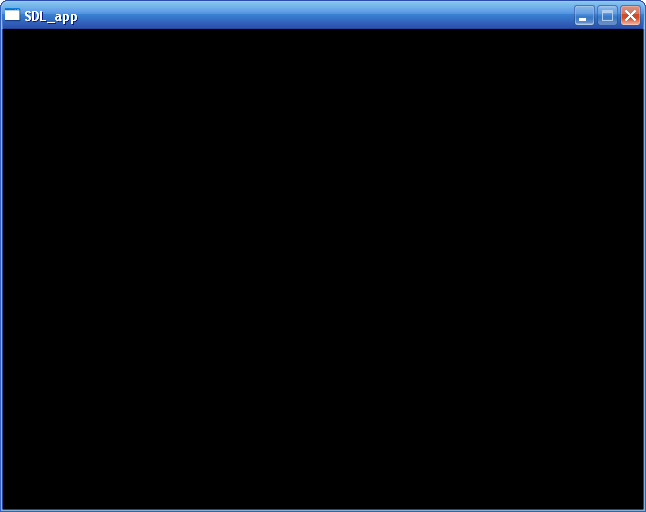
\includegraphics[width=0.8\textwidth]{Chapter_III-2_Empty-window}
\end{figure}

ها قد وصلنا !

إن أردت، قم بوضع العَلم الذي يسمح بتعديل مقاييس النافذة. للعِلْم، في ألعاب الفيديو نفضّل النوافذ ذات الأبعاد الثابتة (لأنه يسهل التعامل معها)، إذا فلنترك النافذة ثابتة كما هي الآن.

\begin{warning}
احذر من العَلَم 
\InlineCode{SDL\_FULLSCREEN}
الخاص بوضع الشاشة الكاملة، و من العَـلم 
\InlineCode{SDL\_NOFRAME}
الذي يقوم بإخفاء حواشي النافذة. بما أنّه لن يكون هناك شريط للعنوان، فلن نكون قادرين على الخروج من البرنامج، إلا بالاستعانة بالمعالج !\\
تريّث قليلاً حتى نتعلّم معالجة الأحداث (في الفصول القادمة) و ستتمكن بعدها من الخروج من النافذة بطريقة أقل عنفاً من استدعاء المعالج.
\end{warning}

\subsection{تغيير عنوان النافذة}

لحدّ الآن، النافذة أخذت عنوانا تلقائيا (و هو 
\InlineCode{SDL\_app}
في الصورة السابقة).\\
هل تريد تغييره ؟

إن الأمر بسيط للغاية، يكفي استعمال الدالة
\InlineCode{SDL\_WM\_SetCaption}.\\
هذه الدالة تأخذ معاملين : المعامل الأول هو العنوان الذي تريد إعطاءه للنافذة، و المعامل الثاني هو العنوان الذي تريد إعطاءه للأيقونة.

خلافاً لما يعتقده الجميع، تغيير اسم الأيقونة لا يعني تغيير صورة الأيقونة التي تظهر أعلى يسار النافذة. هذا لا يعمل دائما (حسب معرفتي، قد يعطي نتائج على الـ\textenglish{GNU/Linux}
في بيئة الـ\textenglish{Gnome}).
شخصياً، أنا أبعث القيمة
\InlineCode{NULL}
إلى الدالة. على أية حال، يمكننا تغيير شكل الأيقونة التي تظهر أعلى يسار النافذة، لكننا سنتعلّم ذلك في الفصل القادم، لأنّ هذا الأمر ليس بمستواك بعد.

هذه نفس الـ\InlineCode{main}
السابقة، مع إضافة الدالة
\InlineCode{SDL\_WM\_SetCaption} :

\begin{Csource}
int main(int argc, char *argv[])
{
	SDL_Init(SDL_INIT_VIDEO);
	SDL_SetVideoMode(640, 480, 32, SDL_HWSURFACE);
	SDL_WM_SetCaption("My super SDL window !", NULL);
	pause();
	SDL_Quit();
	return EXIT_SUCCESS;
}
\end{Csource}

\begin{information}
لاحظ بأنني استعملت القيمة 
\InlineCode{NULL}
للمعاملات غير المهمة بشكل كبير. بالنسبة للـ\textenglish{C}،
يجب أن يتم إعطاء قيم لكل المعاملات التي تستقبلها الدوال، حتى لو كانت هذه المعاملات غير مهمة لك، فأعطها
\InlineCode{NULL}
كما فعلت أنا هنا. بينما الـ\textenglish{C++}
تسمح بألا نعطي أساساً قيمة لبعض المعاملات الاختياريّة عندما نستدعي الدوال.
\end{information}

للنافذة الآن عنوان.

\begin{figure}[H]
	\centering
	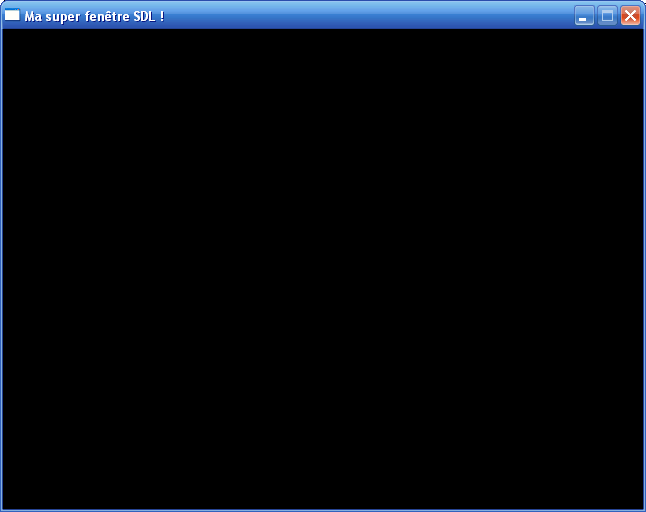
\includegraphics[width=0.8\textwidth]{Chapter_III-2_Window-title}
\end{figure}

\section{التعامل مع المساحات}

لحد الآن تمكّنا من فتح نافذة ذات خلفيّة سوداء. ما نريد الآن هو أن نملأها ببعض الأشياء، أي أن "نرسم" فيها.

كما قلت لك في الفصل السابق، فإن المكتبة
\textenglish{SDL}
هي مكتبة منخفضة المستوى، أي أنها لا توفّر لنا سوى دوال قاعدية، بسيطة جداً.\\
الصراحة هي أن الشكل الوحيد الذي تسمح لنا الـ\textenglish{SDL}
برسمه هو المستطيل ! كلّ ما سنقوم به هو جمع بعض المستطيلات في نافذة. نسمّي هذه المستطيلات بـ\textbf{المساحات}
(\textenglish{Surfaces})،
المساحة هي الوحدة الرسومية القاعدية في الـ\textenglish{SDL}.

\begin{information}
إنه من الممكن أن نرسم أشياء أخرى، مثل الدوائر و المثلثات، إلخ. و لكن لكي نفعل ذلك، يجب أن نكتب بأنفسنا الدوال الّتي تمكّن من فعل ذلك، برسم تلك الأشكال بيكسلا ببيكسل، و إما أن نستعمل مكتبة أخرى إلى جانب الـ\textenglish{SDL}.
الأمر معقّد نوعاً ما، لكن لا تقلق، ستجد بأننا لسنا بحاجة إلى كلّ هذا في التطبيق.
\end{information}

\subsection{مساحتك الأولى : الشاشة}

في كل برامج الـ\textenglish{SDL}،
توجد على الأقل مساحة عمل واحدة و هي ما نسميه بالشاشة 
(\textenglish{Screen})،
و هي مساحة توافق كل النافذة، أي كلّ المساحة السوداء التي تظهر بالنافذة.

في الشفرة المصدرية، كل مساحة يتم تخزينها في متغير من نوع
\InlineCode{SDL\_Surface}.
نعم، إنه نوع بيانات تم إنشاؤه من طرف الـ\textenglish{SDL}
(هذا المتغير عبارة عن هيكل).

بما أن أول مساحة ننشئها هي الشاشة، فهيا بنا :

\begin{Csource}
SDL_Surface *screen = NULL;
\end{Csource}

تلاحظ أنني قمت بإنشاء مؤشّر. لماذا أفعل هذا ؟ لأن الـ\textenglish{SDL}
هي من ستقوم بحجز مكان في الذاكرة من أجل مساحتنا. المساحة بالفعل ليس لها بالضرورة دائما نفس الحجم و لهذا فعلى الـ\textenglish{SDL}
أن تقوم بحجز حيّ من أجلنا (هنا، هذا يعتمد على حجم النافذة التي فتحناها).

لم أقل لك هذا من قبل، لكن الدالة
\InlineCode{SDL\_SetVideoMode}
تقوم بإرجاع قيمة ! ستقوم بإرجاع مؤشّر نحو المكان بالذاكرة المخصص لمساحة الشاشة.\\
ممتاز، يمكننا إذا استرجاع المؤشّر في المتغير 
\InlineCode{screen} :

\begin{Csource}
screen = SDL_SetVideoMode(640, 480, 32, SDL_HWSURFACE);
\end{Csource}

المؤشّر الآن يمكن أن يساوي إحدى القيمتين :

\begin{itemize}
	\item \InlineCode{NULL} :
	المتغير 
	\InlineCode{screen}
	سيساوي
	\InlineCode{NULL}
	إذا فشلت الدالة
	\InlineCode{SDL\_SetVideoMode}
	في تحميل أسلوب العرض الذي تم طلبه. و هذا يحصل حينما يتم اختيار دقة جد عالية أو عدد كبير جداً من الألوان، أكبر من أقصى عدد يتحمله جهازك.
	\item قيمة أخرى : إذا كانت القيمة مختلفة عن 
	\InlineCode{NULL}،
	فهذا يعني أن الـ\textenglish{SDL}
	قامت بحجز المكان، كل شيء على ما يرام !
\end{itemize}

إنه من المستحسن هنا أن تتم معالجة الأخطاء، تماما مثلما فعلنا حينما أردنا تحميل الـ\textenglish{SDL}،
هاهي إذا الدالة

الكاملة بإضافة معالجة الأخطاء للـ\InlineCode{SDL\_SetVideoMode}.

\begin{Csource}
int main(int argc, char *argv[])
{
	SDL_Surface *screen = NULL; // The pointer which stores the surface of the screen
	SDL_Init(SDL_INIT_VIDEO);
	screen = SDL_SetVideoMode(640, 480, 32, SDL_HWSURFACE); // We try to open the window
	if (screen  == NULL) // If we can't, we note it and we exit.
	{
		fprintf(stderr, "Impossible to load the video mode : %s\n", SDL_GetError());
		exit(EXIT_FAILURE);
	}
	SDL_WM_SetCaption("My super SDL window !", NULL);
	pause();
	SDL_Quit();
	return EXIT_SUCCESS;
}
\end{Csource}

الرسالة التي تتركها لنا الدالة
\InlineCode{SDL\_GetError}،
مفيدة من أجل معرفة ما الّذي لم يعمل.

\begin{information}
حكاية صغيرة : مرة أخطأت بينما أردت أن أفتح نافذة بأسلوب الشاشة الكاملة 
(\textenglish{Full screen})،
في عوض أن أطلب الدقة
$1024 \times 768$
كتبت بالخطأ 
$10244 \times 768$،
لم أفهم لماذا لم يتم التحميل، لأنّي لم أنتبه إلى أنني كتبت 4 مرّتين (ربما كنت متعباً). و لحل المشكل ألقيتُ نظرة على الملف 
\InlineCode{stderr.txt}،
توجهت إلى رسالة الخطأ و اكتشفت بأن الدقة التي طلبتها مرفوضة (شيء يثير الفضول أليس كذلك~؟).
\end{information}

\subsection{تلوين مساحة}

لا توجد 36 طريقة لملء مساحة، الحقيقة أنه توجد طريقتان :

\begin{itemize}
	\item إما أن يتم تلوين المساحة بلون موحّد.
	\item إما أن يتم ملؤها عن طريق تحميل صورة.
\end{itemize}

\begin{information}
يمكنك في الحقيقة الرسم في المساحة بيكسلا ببيكسل، لكن هذه الطريقة معقّدة، لن نراها هنا.
\end{information}

سنرى أولا كيف نقوم بتلوين مساحة بلون موحّد. في الفصل القادم سنتعلّم كيف نقوم بتحميل صورة.

الدالة التي تسمح بتلوين النافذة بلون موحّد هي
\InlineCode{SDL\_FillRect}
(العبارة 
\InlineCode{FillRect}
تعني ملء مستطيل بالإنجليزيّة). هذه الدالة تستقبل 3 معاملات و هي :

\begin{itemize}
	\item مؤشّر نحو المساحة التي نريد التلوين عليها (مثلا
	\InlineCode{screen}).
	\item الجزء من المساحة الذي نريد تلوينه، إذا أردت تلوين كل المساحة (و هذا الّذي نريده) فلتكن قيمة المؤشر 
	\InlineCode{NULL}.
	\item اللون الذي نريد أن نلوّن به المساحة.
\end{itemize}

كملخّص :

\begin{Csource}
SDL_FillRect(surface, NULL, color);
\end{Csource}

\subsubsection{التحكم في الألوان بالـ\textenglish{SDL}}

في الـ\InlineCode{SDL}
كل لون مخزن في عدد من نوع
\InlineCode{Uint32}.

\begin{question}
إذا كان عدداً، لماذا إذا لم نستعمل ببساطة النوع
\InlineCode{int}
أو النوع
\InlineCode{long} ؟
\end{question}

الـ\InlineCode{SDL}
هي مكتبة متعددة المنصات، و كما تعلم فحجم الـ\InlineCode{int}
يتغير من نظام تشغيل إلى آخر. لهذا فإن الـ\InlineCode{SDL}
تقوم باستخدام أعداد من أنواع جديدة، هذه الأنواع الجديدة تحجز نفس المكان بالذاكرة في كل أنظمة التشغيل.\\

هناك مثلاً :

\begin{itemize}
	\item \InlineCode{Uint32} :
عدد صحيح بحجم
\textenglish{32 bits}
أي
\textenglish{4 octets}
(للتذكير :
\textenglish{1 octet = 8 bits}).
	\item \InlineCode{Uint16} :
عدد صحيح مشفر على
\textenglish{16 bits} (\textenglish{2 octets}).
	\item \InlineCode{Uint8} :
عدد طبيعي مشفر على
\textenglish{8 bits} (\textenglish{1 octet}).
\end{itemize}
لن تستعمل المكتبة سوى
\InlineCode{typedef}
لتقوم بتغيير قيمة العدد على حسب نظام التشغيل. إذا كنت فضولياً، فألق نظرة على الملف
\InlineCode{SDL\_types.h}.

لن نتأخر في التعامل مع كل هذا، فالتفاصيل لا تهم حالياً. كل ما عليك تذكره هو أن النوع
\InlineCode{Uint32}
لا يخزن إلا عددا صحيحاً ليس إلا، مثل
\InlineCode{int}.

\begin{question}
لكن كيف أعرف أي عدد يوافق اللون الّذي أريد ؟
\end{question}

هناك بالفعل دالة من أجل ذلك :
\InlineCode{SDL\_MapRGB}،
هذه الأخيرة تستقبل 4 معاملات :

\begin{itemize}
	\item صيغة الألوان : هذه الصيغة تعتمد على عدد
	\textenglish{bits/pixel}
	التي قد طلبتها بالـ\InlineCode{SDL\_SetVideoMode}.
	يمكنك استرجاع القيمة فهي موجودة في المتغير الداخلي
	\InlineCode{screen->format}.
	\item كمية الأحمر في اللون.
	\item كمية الأخضر في اللون.
	\item كمية الأزرق في اللون.
\end{itemize}

قد لا يعرف البعض بأن كل الألوان يتم تشكيلها عن طريق خلط الألوان : أزرق، أحمر و أخضر.\\
كل كمية تتدرج من العدد 0 (لا يوجد لون) إلى العدد 255 (كل اللون موجود). أي أننا لو كتبنا :

\begin{Csource}
SDL_MapRGB(screen->format, 255, 0, 0)
\end{Csource}

فاللون المتشكل سيكون أحمرا. لا وجود للأخضر و لا للأزرق، أما لو نكتب :
\begin{Csource}
SDL_MapRGB(screen->format, 0, 0, 255)
\end{Csource}
اللون سيكون أزرقا، بينما لو نكتب :
\begin{Csource}
SDL_MapRGB(screen->format, 255, 255, 255)
\end{Csource}

اللون سيكون أبيضا لأننا دمجنا كل الألوان، لو أنك تريد تشكيل اللون الأسود، فلتجعل كل القيم على 0.

\begin{question}
ألا يمكننا استعمال لون آخر غير هذه الألوان ؟
\end{question}

كلّا، يمكنك ذلك لو أنك تقوم بمزج الألوان بشكل ذكي. للمساعدة في ذلك، توجه إلى برنامج
\textenglish{Paint}
ثم إلى
\InlineCode{Colors} / \InlineCode{Modify the colors}،
انقر على
\InlineCode{Define the colors}
ثم
\InlineCode{Custom}.\\
هنا، اختر اللون الّذي يلائمك. أنظر إلى الصورة التالية :

\begin{figure}[H]
	\centering
	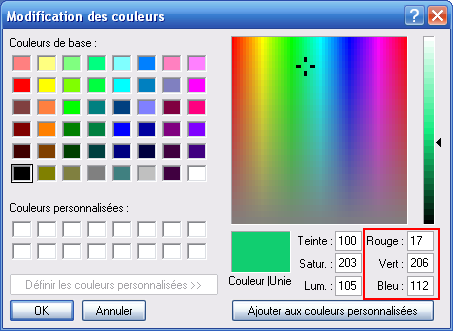
\includegraphics[width=0.7\textwidth]{Chapter_III-2_Colors}
\end{figure}

مركّبات اللون متواجدة في أسفل يمين النافذة. كما ترى فقد اخترت لونا أخضر مزرقّا، و هو يتكوّن من 17 من الأحمر، 206 من الأخضر، و 112 من الأزرق.
\subsubsection{تلوين الشاشة}

الدالة
\InlineCode{SDL\_MapRGB}
تقوم بإرجاع عدد من نوع
\InlineCode{Uint32}
يوافق اللّون المختار.\\
يمكننا إذا تعريف متغير باسم
\InlineCode{blueGreen}
يحوي الشفرة الخاصة لاسترجاع هذا اللون :

\begin{Csource}
Uint32 blueGreen = SDL_MapRGB(screen->format, 17, 206, 112);
\end{Csource}

ليس من الضروري المرور دائما على متغير لتخزين اللون المراد استعماله (إلا إن كنت تحتاجه فعلا في برنامجك).\\
يمكنك مباشرة إعطاء القيمة التي تم ارجاعها من طرف الدالة
\InlineCode{SDL\_MapRGB}
إلى الدالة
\InlineCode{SDL\_FillRect}.

لو نريد أن نملأ الشاشة باللون الأخضر المزرق، يمكننا كتابة :

\begin{Csource}
SDL_FillRect(screen , NULL, SDL_MapRGB(screen->format, 17, 206, 112));
\end{Csource}

لقد قمنا باستدعاء دالة خلال استدعاء دالة أخرى، أعتقد أنك تعرف بأن الأمر ممكن و لا يسبب أيّ مشاكل في لغة
\textenglish{C}.

\subsubsection{تحديث الشاشة}

لقد اقتربنا من تحقيق الهدف.\\
لقد نسينا أمراً بسيطاً : و هو الأمر بتحديث الشاشة. بالفعل، فالأمر 
\InlineCode{SDL\_FillRect}
يقوم بتلوين الشاشة، لكن هذا لا يحصل إلا في الذاكرة، إذ يجب أن نطلب من الحاسوب تحديث الشاشة لاستعمال البيانات الجديدة.

من أجل هذا سنستعمل الدالة 
\InlineCode{SDL\_Flip}،
سنتكلم بشكل مفصل عن هذه الدالة لاحقا.\\
الدالة تستقبل معاملا واحدا و هو الشاشة
\InlineCode{screen}.

\subsubsection{فلنلخّص كل شيء !}

هذه دالة
\InlineCode{main}
تقوم بفتح نافذة ملونة باللون الأخضر المزرق :

\begin{Csource}
int main(int argc, char *argv[])
{
	SDL_Surface *screen = NULL;
	SDL_Init(SDL_INIT_VIDEO);
	screen = SDL_SetVideoMode(640, 480, 32, SDL_HWSURFACE);
	SDL_WM_SetCaption("My super SDL window !", NULL);
	// We colorize the screen with blue-green color
	SDL_FillRect(screen, NULL, SDL_MapRGB(screen->format, 17, 206, 112));
	SDL_Flip(screen); 
	pause();
	SDL_Quit();
	return EXIT_SUCCESS;
}
\end{Csource}

هاهي النتيجة :

\begin{figure}[H]
	\centering
	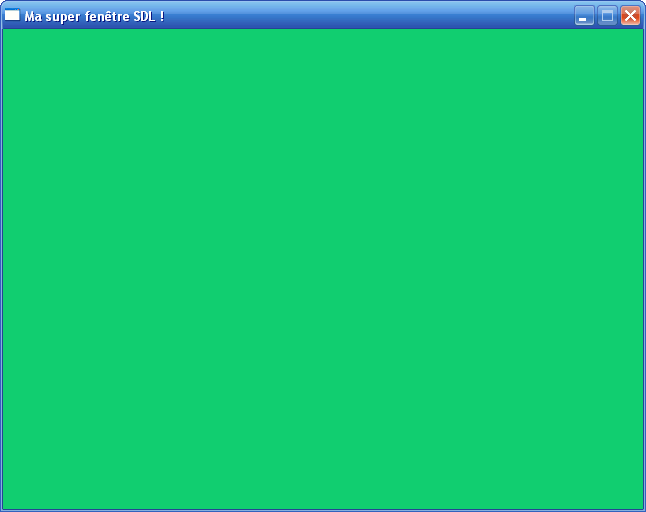
\includegraphics[width=0.8\textwidth]{Chapter_III-2_Window-color}
\end{figure}

\subsection{رسم مساحة أخرى في الشاشة}

النتيجة السابقة جيدة، لكننا لن نتوقف هنا. لحد الآن ليست لدينا سوى مساحة واحدة و هي الشاشة. نحن نريد أن نقوم بالرسم عليها، أي "نلصق" مساحات أخرى عليها بألوان مختلفة.

لهذا يجب علينا إنشاء متغير من نوع
\InlineCode{SDL\_Surface}
للمساحة الجديدة :

\begin{Csource}
SDL_Surface *rectangle = NULL;
\end{Csource}

سنطلب إذا من الـ\InlineCode{SDL}
أن تقوم بحجز مكان في الذاكرة من أجل المساحة الجديدة.\\
من أجل الشاشة كنا قد استعملنا
\InlineCode{SDL\_SetVideoMode}.
لكن هذه الأخيرة لا تعمل إلا على  الشاشة (المساحة الرئيسية)، لا نريد أن نقوم بإنشاء نافذة من أجل كل مستطيل نريد إنشاءه !

توجد إذا دالة أخرى من أجل إنشاء مساحة : 
\InlineCode{SDL\_CreateRGBSurface}.
هذه هي التي سنقوم باستعمالها في كل مرة نريد أن ننشئ مساحة جديدة.

هذه الدالة تستقبل العديد من المعاملات (ثمانية !). لكنني لن أتطرّق إلا للمعاملات التي تهمّنا لحدّ الآن.\\
بما أن لغة 
\textenglish{C}
تُلزمنا بإدخال قيم لكل المعاملات، فإننا سنقوم بوضع القيمة 0 في مكان كل معامل لا يهمّنا.

فلنتأمل قليلا في المعاملات الأربع الأولى (يجدر بها أن تذكّرنا بإنشاء الشاشة).

\begin{itemize}
	\item قائمة الأعلام (الخيارات). لديك الاختيار بين :
	\begin{itemize}
		\item \InlineCode{SDL\_HWSURFACE} :
		المساحة يتم تحميلها في الذاكرة الرسوميّة. و هي تحتوي على مكان أقل مقارنة بالذاكرة الخاصة بالنظام (حقيقة، مع بطاقات الـ\textenglish{3D}
		في أيامنا هذه، قد لا يكون لهذا تأثير)، لكنها ذاكرات سريعة و فعّالة.
		\item \InlineCode{SDL\_SWSURFACE} :
		يتم تحميل المساحة في الذاكرة الخاصة بالنظام، أين يوجد الكثير من المكان، لكن هذا الاختيار سيجبر المعالج على القيام بحسابات أكثر. لو أنك حمّلت المساحة على الذاكرة الرسوميّة، فإن البطاقة 
		\textenglish{3D}
		هي المسؤولة عن القيام بأغلب الحسابات.
	\end{itemize}
	\item عرض المساحة (\textenglish{pixels}).
	\item ارتفاع المساحة (\textenglish{pixels}).
	\item عدد الألوان (\textenglish{bits/pixel}).
\end{itemize}

هكذا إذا نقوم بحجز مكان للمساحة الجديدة في الذاكرة :

\begin{Csource}
rectangle = SDL_CreateRGBSurface(SDL_HWSURFACE, 220, 180, 32, 0, 0, 0, 0);
\end{Csource}

الأربع معاملات الأخيرة تساوي 0، كما قلت لك، لأننا لا نهتم بأمرها حالياً. 

بما أننا قمنا بالحجز اليدوي للذاكرة، فيجب علينا تحريرها باستعمال الدالة 
\InlineCode{SDL\_FreeSurface}
و التي نستعملها قبل 
\InlineCode{SDL\_Quit} :

\begin{Csource}
SDL_FreeSurface(rectangle);
SDL_Quit();
\end{Csource}

\begin{information}
ليس هناك من داعٍ إلى تحرير المساحة
\InlineCode{screen}
باستعمال
\InlineCode{SDL\_FreeSurface}
لأنه يتم تحريرها تلقائياً عند استدعاء
\InlineCode{SDL\_Quit}.
\end{information}

يمكننا الآن تلوين المساحة الجديدة باللون الأبيض مثلا :

\begin{Csource}
SDL_FillRect(rectangle, NULL, SDL_MapRGB(screen->format, 255, 255, 255));
\end{Csource}

\subsubsection{لصق المساحة بالشاشة}

اقتربنا من النهاية، هيا بعض الشجاعة ! المساحة جاهزة، لكن لو تحاول تجريب البرنامج، ستلاحظ أنها لن تظهر على الشاشة، بالفعل إذ أن المساحة
\InlineCode{screen}
هي وحدها التي تم إظهارها. لكي نستطيع رؤية مساحتنا الجديدة يجب أن نقوم بـ\textbf{تسوية}
المساحة، أي لصقها على الشاشة، سنستعمل لأجل هذا الدالة 
\InlineCode{SDL\_BlitSurface}.
 هذه الدالة تنتظر :
 
\begin{itemize}
	\item المساحة التي نريد لصقها (هنا 
	\InlineCode{rectangle}).
	\item معلومة حول الجزء من تلك المساحة الذي نريد لصقه (اختياري). لن يهمنا الأمر الآن فنحن نريد لصق كل المساحة و لهذا فستكون القيمة
	\InlineCode{NULL}.
	\item المساحة التي نريد أن نلصق عليها المساحة الجديدة (في حالتنا هذه نتكلم عن الشاشة 
	\InlineCode{screen}).
	\item مؤشّر نحو متغير يحتوي الإحداثيّات. هذه الإحداثيات تشير إلى المكان الذي نريد أن نلصق عليه المساحة، أي موقعه.
	
للإشارة إلى الإحداثيّات، نحتاج إلى استعمال متغير من نوع 
\InlineCode{SDL\_Rect}.\\
إنّه هيكل يحتوي العديد من المركّبات، إثنتان منها تهمّنا :
	\begin{itemize}
		\item \InlineCode{x} : 
الفاصلة.
		\item \InlineCode{y} : 
الترتيبة. 
	\end{itemize}	
\end{itemize}

يجب أن تعرف أن الإحداثيّة
\InlineCode{(0, 0)}
توافق أقصى نقطة في يسار أعلى الشاشة.\\
أما الإحداثيّة 
\InlineCode{(640, 480)}
فهي توافق النقطة الموجودة في أقصى يمين أسفل الشاشة، و هذا إن كنت قد فتحت نافذة بحجم
$640 \times 480$
مثلي.

هذا المخطط سيساعدك في الفهم  :

\begin{figure}[H]
	\centering
	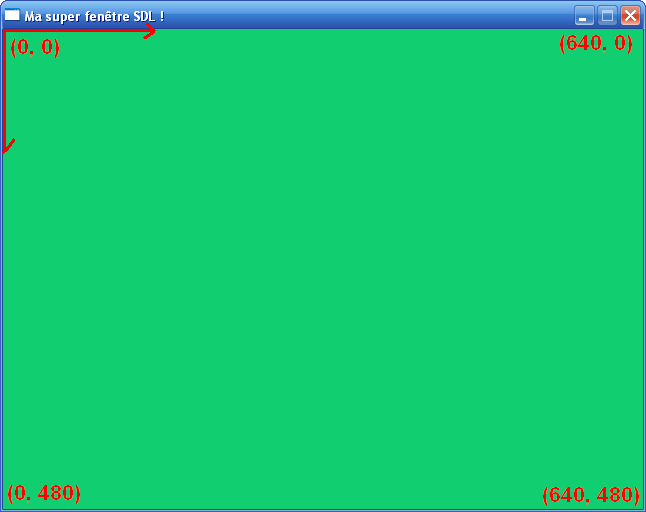
\includegraphics[width=0.8\textwidth]{Chapter_III-2_Window-coordinates}
\end{figure}

إذا كنت قد درست الرياضيات من قبل، فعلى الأرجح لن تضيع بينما تحاول  فهم كيفية العمل. فلننشئ إذا متغيرا 
\InlineCode{position}.
سنعطي القيمة 0 لكل من الفاصلة و الترتيبة و ذلك ليتم لصق مساحتنا (المستطيل) في أعلى يسار النافذة :

\begin{Csource}
SDL_Rect position;
position.x = 0;
position.y = 0;
\end{Csource}

و الآن بما أننا حددنا موقعنا في النافذة، يمكننا تسوية المساحة الجديدة على الشاشة :

\begin{Csource}
SDL_BlitSurface(rectangle, NULL, screen, &position);
\end{Csource}
 
لاحظ أنني استعملت الرمز
\InlineCode{\&}
و ذلك لأنه يجب علينا إرسال عنوان المتغير
\InlineCode{position}.

\subsubsection{تلخيص الشفرة المصدرية}

أعتقد أن وضع الشفرة المصدرية الّتي تلخص ما شرحته لن يكون مضراً :

\begin{Csource}
int main(int argc, char *argv[])
{
	SDL_Surface *screen = NULL, *rectangle = NULL;
	SDL_Rect position;
	SDL_Init(SDL_INIT_VIDEO);
	screen = SDL_SetVideoMode(640, 480, 32, SDL_HWSURFACE);
	// Surface allocation
	rectangle = SDL_CreateRGBSurface(SDL_HWSURFACE, 220, 180, 32, 0,0, 0, 0);
	SDL_WM_SetCaption("My super SDL window !", NULL);
	SDL_FillRect(screen, NULL, SDL_MapRGB(screen->format, 17, 206,112));
	position.x = 0; // The coordinates of the surface will be (0, 0)
	position.y = 0;
	// Filling the surface with white color
	SDL_FillRect(rectangle, NULL, SDL_MapRGB(screen->format, 255,255, 255));
	SDL_BlitSurface(rectangle, NULL, screen, &position); // Sticking the surface on the screen 
	SDL_Flip(screen); // Updating the screen
	pause();
	SDL_FreeSurface(rectangle); // Freeing the surface
	SDL_Quit();
	return EXIT_SUCCESS;
}
\end{Csource}

شاهد النتيجة :

\begin{figure}[H]
	\centering
	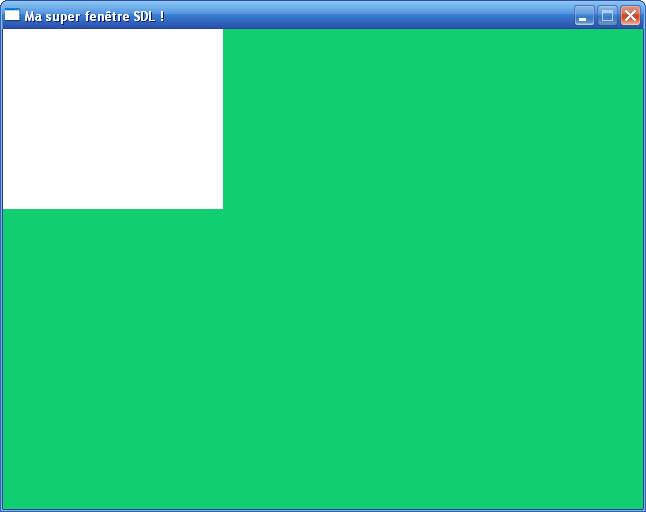
\includegraphics[width=0.8\textwidth]{Chapter_III-2_Colors-paste}
\end{figure}

\subsubsection{مركزةُ المساحة في الشاشة}

نحن نجيد إظهار المساحة في أعلى اليسار. يسهل أيضا موقعتها أسفل يمين الشاشة. ستكون الإحداثيات
\mbox{($640 - 220, 480 - 180$)}،
لأنه يجب إنقاص حجم المستطيل ليتم إظهاره كاملا. 

لكن كيف تتم مركزةُ المستطيل الأبيض ؟ لو تفكّر قليلاً ستجد بأن الحساب
\textit{رياضياتيّ}.
فهنا نعرف الهدف من الرياضيات و الحساب الهندسي !\\
كلّ هذا الأمر بمستوى سهل هنا :

\begin{Csource}
position.x = (640 / 2) - (220 / 2);
position.y = (480 / 2) - (180 / 2);
\end{Csource}

فاصلة المستطيل هي نصف عرض الشاشة
($640 / 2$).
و لكن، بالإضافة إلى هذا، يجب أن يتم إنقاص نصف طول المستطيل أيضاً 
($220 / 2$)،
لأنك إن لم تنقص هذا الحجم، سيكون تمركز المستطيل خاطئاً (جرّب عدم فعل ذلك و ستفهم ما الّذي أعنيه).\\
كذلك بالنسبة للترتيبة مع ارتفاع الشاشة و المستطيل.

النتيجة : المستطيل الأبيض يتمركز بشكل جيد في الشاشة.

\begin{figure}[H]
	\centering
	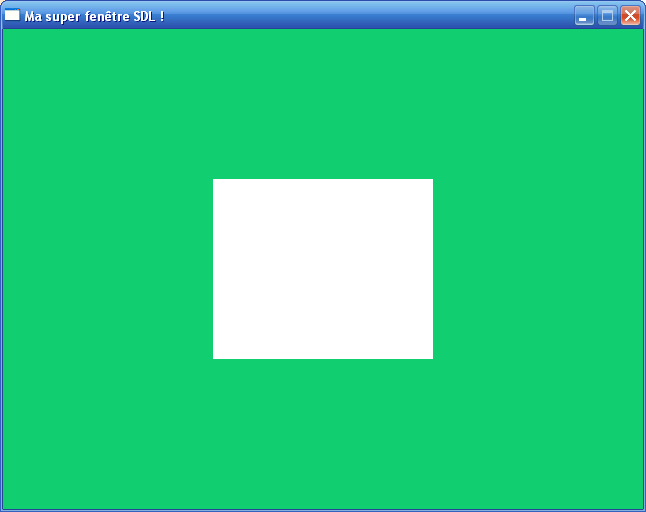
\includegraphics[width=0.8\textwidth]{Chapter_III-2_Window-color-centered}
\end{figure}

\section{تمرين : إنشاء تدرّج لونيّ}

سننهي الفصل بتمرين صغير (مصحّح) متبوع بسلسلة تمارين أخرى (غير مصححة من أجل حثّك على التدريب).

التمرين المصحح ليس صعباً حقّا : ما نريد إنشاءه هو نافذة متدرّجة الألوان عموديا من الأسود إلى الأبيض.\\
سيكون عليك إنشاء 255 مساحة بارتفاع 1 بيكسل. كل مساحة لها لون مختلف أكثر فأكثر سوادا.

هذا ما يجب عليك الحصول عليه في النهاية، صورة مشابهة لهذه :

\begin{figure}[H]
	\centering
	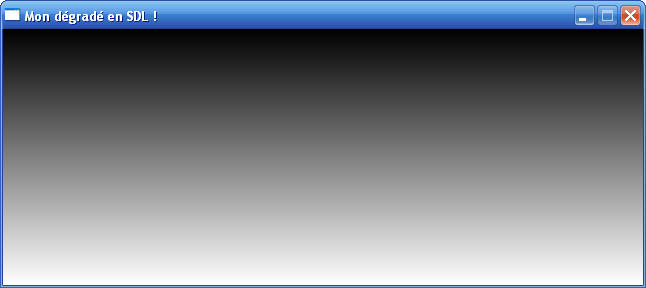
\includegraphics[width=0.8\textwidth]{Chapter_III-2_Window-gradient}
\end{figure}

 إنه أمر جميل، أليس كذلك ؟ الشيء الأجمل هو أن بعض الحلقات التكرارية كافية من أجل تحقيق المطلوب.
 
لفعل ذلك يجب إنشاء 256 مساحة (أي 256 سطر) تحتوي مركبات الألوان (أحمر، أخضر، أزرق) التالية~:

\begin{Csource}
0, 0, 0) // Black
(1, 1, 1) // Gray that is so so close from black
(2, 2, 2) // Gray that is so close from black
...
(128, 128, 128) // Medium gray (to 50 %)
...
(253, 253, 253) // Gray that is so  close from white
(254, 254, 254) // Gray that is so so close from white
(255, 255, 255) // White
\end{Csource}

يجب على أيّ كان أن يعرف أنّه بحاجة إلى حلقة تكراريّة للقيام بهذا (لن تسعد بتكرار 256 سطرا !). و لهذا سنقوم بإنشاء جدول من نوع 
\InlineCode{SDL\_Surface*}
من 256 خانة.

إلى العمل. لديك 5 دقائق !

\subsection{تصحيح !}
 
يجب أولا أن نقوم بتعريف جدول من 256
\InlineCode{SDL\_Surface*}.
سنهيّؤه على
\InlineCode{NULL} :

\begin{Csource}
SDL_Surface *lines[256] = {NULL};
\end{Csource}

سنعرف متغيراً
\InlineCode{i}
من أجل الحلقات 
\InlineCode{for}.

سنغيّر أيضاً ارتفاع النافذة لكي تكون مناسبة للعمل. إذ سنعطيها 256 بيكسلز كارتفاع، و ذلك من أجل عرض كل سطر من بين 256 سطرا.

سنستعمل بعد ذلك حلقة تكرارية
\InlineCode{for}
من أجل حجز مكان لـ256 مساحة الّتي تم إنشاؤها. الجدول سيستقبل 256 مؤشّرا إلى كلّ واحد من المساحات المنشأة :

\begin{Csource}
for (i = 0 ; i <= 255 ; i++)
	lines[i] = SDL_CreateRGBSurface(SDL_HWSURFACE, 640, 1, 32, 0,0, 0, 0);
\end{Csource}

بعد ذلك نقوم بملء و لصق كل مساحة في الشاشة واحدة بواحدة.

\begin{Csource}
for (i = 0 ; i <= 255 ; i++)
{
	position.x = 0; // The lines are to the left (0 abscissa)
	position.y = i; // The vertical position depends on the line's number
	SDL_FillRect(lines[i], NULL, SDL_MapRGB(screen->format, i, i, i)); // Drawing
	SDL_BlitSurface(lines[i], NULL, screen, &position); // Sticking
}
\end{Csource}

 لاحظ أنني استعمل كل الوقت المتغير 
\InlineCode{position}.
إذ ليس لازما أن ننشئ 256 واحدا، لأننا لن نقوم إلا ببعث المتغير إلى الدالة 
\InlineCode{SDL\_BlitSurface}.
يمكننا إذن إعادة استخدامه دون مشاكل.\\
في كلّ مرة أقوم بالتعديل على الترتيبة
(\InlineCode{y})،
لتسوية المساحة على الارتفاع الصحيح. اللون يعتمد في كلّ مرة على قيمة المتغير
\InlineCode{i}
(ستكون
$0, 0, 0$
في أوّل مرّة و $255, 255, 255$ في آخر مرّة).

\begin{question}
لكن لماذا قيمة 
\InlineCode{x}
هي 0 دائماً ؟\\
كيف يمكن للمساحة أن تتلون كليا إذا كانت قيمة الـ\InlineCode{x}
دائما 0 ؟
\end{question}

المتغير
\InlineCode{position}
يشير إلى أي مكان تتواجد فيه المنطقة أعلى اليسار (هنا نتكلم عن السطر). هي لا تحدد عرض المساحة و إنما فقط أين تتواجد المركّبة على الشاشة.\\
بما أن كل الأسطر تبدأ في أقصى يسار النافذة، فستكون الفاصلة مساوية لـ0. حاول وضع فاصلة تساوي 50 لترى ماذا سيعطيك : كل الأسطر ستتنحي إلى اليمين.\\
بما أن المساحة تأخذ 640 بيكسل كطول ، فإن الـ\textenglish{SDL}
تقوم بإنشاء 640 بيكسلا في اتجاه اليمين (من نفس اللون) إنطلاقاً من المركبات التي يشير إليها المتغير 
\InlineCode{position}.

في المخطط التالي أريك مركبات النقطة المتواجدة أعلى يسار الشاشة (وضعية أول سطر) ومركبات النقطة المتواجدة أسفل يسار الشاشة (وضعية آخر سطر).

\begin{figure}[H]
	\centering
	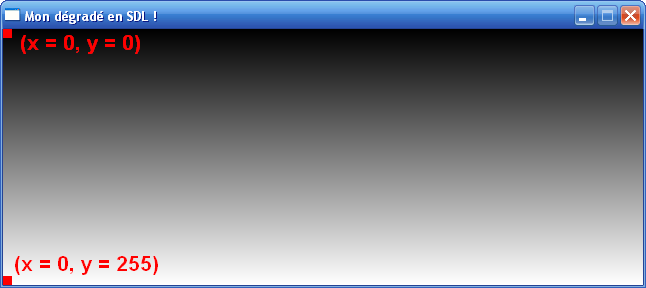
\includegraphics[width=0.8\textwidth]{Chapter_III-2_Window-gradient-coordinates}
\end{figure}

كما ترى، من الأعلى إلى الأسفل، المحور لا يتغير 
(\InlineCode{x}
يبقى مساويا لـ0) بينما 
\InlineCode{y}
وحده يتغير من أجل كل سطر جديد، و بهذا 
\InlineCode{position.y = i;}.

أخيراً لا تنس أنه يجب تحرير الذاكرة من أجل كل مساحة من الـ256 مساحة المنشأة، بمساعدة حلقة بالطبع.

\begin{Csource}
for (i = 0 ; i <= 255 ; i++) // Don't forget to free the 256 surfaces
	SDL_FreeSurface(lines[i]);
\end{Csource}

\subsubsection{ملخّص \texttt{main}}

هذه هي الدالة
\InlineCode{main}
كاملة :

\begin{Csource}
int main(int argc, char *argv[])
{
	SDL_Surface *screen = NULL, *lines[256] = {NULL};
	SDL_Rect position;
	int i = 0;
	SDL_Init(SDL_INIT_VIDEO);
	screen = SDL_SetVideoMode(640, 256, 32, SDL_HWSURFACE);
	for (i = 0 ; i <= 255 ; i++)
		lines[i] = SDL_CreateRGBSurface(SDL_HWSURFACE, 640, 1, 32,0, 0, 0, 0);
	SDL_WM_SetCaption("My SDL gradient !", NULL);
	SDL_FillRect(screen , NULL, SDL_MapRGB(screen ->format, 0, 0, 0));
	for (i = 0 ; i <= 255 ; i++)
	{
		position.x = 0; // The lines are to the left
		position.y = i; // The vertical position depends on the line's number
		SDL_FillRect(lines[i], NULL, SDL_MapRGB(screen->format, i, i, i));
		SDL_BlitSurface(lines[i], NULL, screen, &position);
	}
	SDL_Flip(screen);
	pause();
	for (i = 0 ; i <= 255 ; i++) // Don't forget to free the 256 surfaces
		SDL_FreeSurface(lines[i]);
	SDL_Quit();
	return EXIT_SUCCESS;
}
\end{Csource}

{\large"أريد تمارين للتدريب !"}

لا مشكلة، مولّد التمارين مُشَغّل !

\begin{itemize}
	\item قم بإنشاء تدرج عكسي للألوان، أي من الأبيض للأسود. هذا الأمر لن يكون صعبا للبدأ !
	\item يمكنك أيضاً وضع كلى التدرّجين، من الأبيض للأسود ثم من الأسود للأبيض (ستأخذ النافذة ضعف الارتفاع الحالي).
	\item أكثر صعوبة قليلا، يمكنك وضع تدرج أفقي بدل التدرج العمودي.
	\item حاول إنشاء تدرج ألوان مختلفة عن الأسود و الأبيض. جرب مثلا من الأحمر إلى الأسود، من الأخضر إلى الأسود، و من الأزرق إلى الأسود، ثمّ من الأحمر إلى الأبيض، إلخ.
\end{itemize}

\section*{ملخّص}

\begin{itemize}
	\item يتم تحميل الـ\InlineCode{SDL}
	بواسطة الـ\InlineCode{SDL\_Init}
	في بداية البرنامج، و يتم إيقافها باستعمال
	\InlineCode{SDL\_Quit}
	في النهاية.
	\item الأعلام هي ثوابت يمكن جمعها فيما بينها باستعمال الرمز 
	\InlineCode{|}،
	 و هي تلعب دور الخواص.
	\item تقوم الـ\textenglish{SDL}
	بالتعامل مع المساحات و التي هي عبارة عن مستطيلات من نوع 
	\InlineCode{SDL\_Surface}.
	الرسم على النافذة يتم بالاستعانة بهذه المساحات.
	\item توجد دائما على الأقل مساحة واحدة و التي تحجز كلّ النافذة، و نسميها في أغلب الأحيان الشاشة 
	(\InlineCode{screen}).
	\item ملء مساحة يتم باستعمال
	\InlineCode{SDL\_FillRect}،
	ولصقها في الشاشة يتم باستعمال
	\InlineCode{SDL\_BlitSurface}.
	\item الألوان معرّفة بمزيج من الأحمر، الأزرق و الأخضر.
\end{itemize}

  \chapter{إظهار صور}

لقد تعلّمنا كيف نقوم بتحميل الـ\textenglish{SDL}،
فتح نافذة و التعامل مع المساحات. إنها بالفعل من المبادئ التي تجب معرفتها عن هذه المكتبة. لكن لحدّ الآن لا يمكننا سوى إنشاء مساحات موحّدة اللون، و هذا الأمر بدائي قليلاً.

في هذا الفصل، سنتعلّم كيف نقوم بتحميل صور على مساحات، مهما كانت صيغتها
\textenglish{BMP}،
\textenglish{PNG}
أو حتى 
\textenglish{GIF}
أو 
\textenglish{JPG}.
التحكم في الصور أمر مهم للغاية لأنه بتجميع الصور (نسميها أيضاً 
"\textenglish{sprites}")
نضع اللبنات الأولى في بناء لعبة فيديو.

\section{تحميل صورة \textenglish{BMP}}

الـ\textenglish{SDL}
هي مكتبة بسيطة جداً. فهي لا تستطيع أساسا تحميل سوى صور من نوع
"\textenglish{bitmap}"
(ذات امتداد
\InlineCode{.bmp}).
لا تقلق، فبفضل إضافة خاصّة بالـ\textenglish{SDL}
(المكتبة
\textenglish{SDL\_Image})،
 سنرى بأنه بإمكاننا أيضاً تحميل صور من صيغ أخرى.
 
 للبدأ، سنكتفي الآن بما تسمح لنا به الـ\textenglish{SDL}
 بشكل قاعدي. سنقوم بدراسة تحميل صور
\textenglish{BMP}.

\subsection{الصيغة \textenglish{BMP}}

الصيغة
\textenglish{BMP}
(اختصار لـ\textenglish{bitmap})
هي صيغة صور.\\
الصور الّتي نجدها في الحاسوب مخزّنة في ملفات. يوجد العديد من صيغ الصور، أي العديد من الطرق لتخزين صورة في ملف. على حسب الصيغة، يمكن للصورة أخذ الكثير أو القليل من مساحة القرص الصلب، و تملك جودة أحسن أو أسوء.

الـ\textenglish{Bitmap}
هي صيغة غير مضغوطة (على عكس الـ\textenglish{JPG}، \textenglish{PNG}، \textenglish{GIF}،
إلخ).
فعليّا، هذا يعني الأمور التالية~:

\begin{itemize}
	\item يكون الملف سريعاً جداً من ناحية قراءته، على عكس الصيغ المضغوطة التي يجب أن يتم فك الضغط عنها، مما يكلّفنا بعض الوقت.
	\item جودة الصورة مثالية. بعض الصيغ المضغوطة (أفكّر في الـ\textenglish{JPG}
	خصوصا، لأن الـ\textenglish{PNG}
	و الـ\textenglish{GIF}
	لا يغيّرون في الصورة) تقوم بتخريب جودة الصورة، و هذا ليس هو الحال بالنسبة للـ\textenglish{BMP}.
	\item لكنّ الملف سيكون ضخماً بما أنه ليس مضغوطاً !
\end{itemize}

توجد هناك إذا مزايا و مساوئ.\\
بالنسبة للـ\textenglish{SDL}،
الشيء الجيد هو أن نوع الملف سيكون بسيطا و سهل القراءة. إذا كان عليك تحميل الصور دائما في نفس وقت تشغيل برنامجك، من المستحسن استعمال صور بصيغة 
\textenglish{BMP}.
سيكون حجم الملف ضخما حتما، لكنه يـُحمّل بشكل أسرع من الـ\textenglish{GIF}
مثلاً. سيكون الأمر مهّما إذا كان على برنامجك تحميل الكثير من الصور في وقت قصير.

\subsection{تحميل صورة \textenglish{Bitmap}}

\subsubsection{تنزيل حزمة الصور}

في هذا الفصل سنقوم بالعمل على كثير من الصور. إذا أردت القيام بتجريب الشفرات بينما أنت تقرأ (و هذا ما يجدر بك فعله !)، فأنصحك بتنزيل حزمة الصور التي تحتوي كل الصور التي نحتاج إليها.

\textenglish{\url{https://openclassrooms.com/uploads/fr/ftp/mateo21/pack_images_sdz.zip} (1 Mo)}

بالطبع، يمكنك استعمال صورك الخاصة. يجب عليك فقط أن تعدّل مقاييس النافذة على حسب مقاييس الصورة.

قم بوضع كل الصور في مجلّد المشروع. سنبدأ أولاّ بالعمل على الصورة 
\InlineCode{lac\_en\_montagne.bmp}.
هي عبارة عن لقطة تم استخلاصها من مشهد ثلاثي الأبعاد مأخوذ من البرنامج الممتاز الخاص بنمذجة المناظر الطبيعية
\textenglish{Vue d'Espri 4}،
و الذي تم إيقاف تسويقه. منذ ذلك، تمّ تغيير اسم البرنامج إلى
\textenglish{Vue}
و تم تطويره كثيراً. لمن يريد معرفة المزيد عنه، يمكنه زيارة الموقع :
\url{http://www.e-onsoftware.com/}.

\subsubsection{تحميل صورة في مساحة}

سنقوم باستعمال دالة تقوم بتحميل صورة ذات صيغة
\textenglish{BMP}
و لصقها في مساحة.\\
هذه الدالة تدعى 
\InlineCode{SDL\_LoadBMP}
و سترى أن استعمالها سهل للغاية :

\begin{Csource}
mySurface = SDL_LoadBMP("image.bmp");
\end{Csource}

الدالة
\InlineCode{SDL\_LoadBMP}
تقوم بتعويض دالتين تعرفهما :

\begin{itemize}
	\item \InlineCode{SDL\_CreateRGBSurface} :
	تقوم بحجز مكان في الذاكرة من أجل تخزين مساحة ذات الحجم المطلوب (تكافئ دالة 
	\InlineCode{malloc}).
	\item \InlineCode{SDL\_FillRect} :
	تقوم بملئ الهيكل بلون موحّد.
\end{itemize}
لماذا تقوم الدالة بتعويض هذين الدالتين ؟ الأمر بسيط :
\begin{itemize}
	\item الحجم الذي نقوم بحجزه في الذاكرة  من أجل المساحة يعتمد على حجم الصورة : اذا كان حجم الصورة هو 
	$250 \times 300$
	فستأخذ المساحة نفس الحجم.
	\item من جهة أخرى، يتم ملأ المساحة بيكسلا ببيكسل بمحتوى الصورة 
	\textenglish{BMP}.
\end{itemize}

فلنكتب الشفرة دون أي تأخير :

\begin{Csource}
int main(int argc, char *argv[])
{
	SDL_Surface *screen = NULL, *backgroundImage = NULL;
	SDL_Rect backgroundPosition;
	backgroundPosition.x = 0;
	backgroundPosition.y = 0;
	SDL_Init(SDL_INIT_VIDEO);
	screen = SDL_SetVideoMode(800, 600, 32, SDL_HWSURFACE);
	SDL_WM_SetCaption("Loading the images on SDL", NULL);
	/* Loading a Bitmap image in a surface */	
	backgroundImage = SDL_LoadBMP("lac_en_montagne.bmp");
	/* We blit on the screen */
	SDL_BlitSurface(backgroundImage, NULL, ecran, &backgroundPosition);
	SDL_Flip(screen);
	pause();
	SDL_FreeSurface(backgroundImage); // We free the surface
	SDL_Quit();
	return EXIT_SUCCESS;
}
\end{Csource}

و بهذا أكون قد أنشأت مؤشّراً نحو مساحة
(\InlineCode{backgroundImage})
و نحو كل المركّبات الموافقة لها
(\InlineCode{backgroundPosition}).\\
تم إنشاء المساحة في الذاكرة و ملؤها من طرف الدالة 
\InlineCode{SDL\_LoadBMP}.\\
نقوم بتسويتها على المساحة 
\InlineCode{screen}
و هذا كلّ شيء ! الصورة التالية توضّح النتيجة :

\begin{figure}[H]
	\centering
	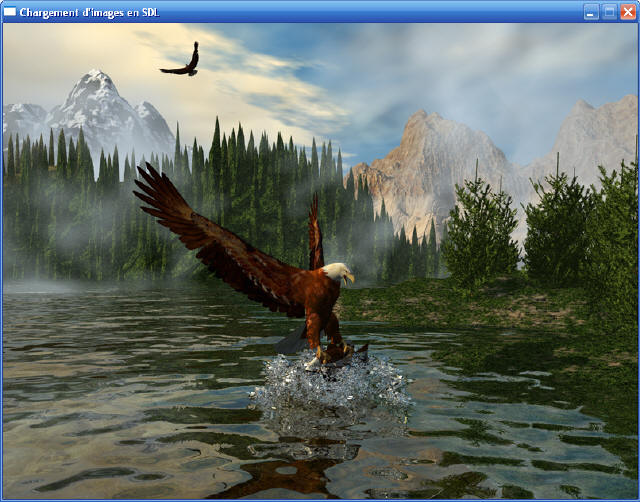
\includegraphics[width=\textwidth]{Chapter_III-3_Window-Image}
\end{figure}

كما ترى، لم يكن الأمر صعباً !

\subsubsection{إرفاق أيقونة بالتطبيق}

بما أننا الآن نجيد تحميل الصور، يمكننا اكتشاف كيفية إرفاق أيقونة بالبرنامج. سيتم إظهار الأيقونة في أعلى يسار النافذة (و أيضاً في شريط المهام). لحدّ الآن نحن لا نملك إلاّ أيقونة افتراضيّة.

\begin{question}
لكن ألا يجدر بأيقونات البرامج أن تكون ذات الامتداد
\InlineCode{.ico} ؟
\end{question}

كلّا، ليس شرطاً ! على كلّ فالامتداد
\InlineCode{.ico}
لا يوجد إلا في نظام
\textenglish{Windows}.
 الـ\textenglish{SDL}
تتعامل مع كلّ أنظمة التشغيل باستعمالها نظاما خاصا بها : المساحة !\\
نعم، أيقونة برنامج 
\textenglish{SDL}
ماهي إلا مساحة بسيطة.

\begin{warning}
يجدر بالأيقونة أن تكون ذات حجم 
$16 \times 16$
بيكسلز. بينما في 
\textenglish{Windows}
يجب أن تكون بحجم
$32 \times 32$
بيكسلز و إلا فستسوء جودتها. لا تقلق إذ يمكن للـ\textenglish{SDL}
"تصغير" أبعاد الصورة لتتمكن من الدخول في 
$16 \times 16$
بيكسلز.
\end{warning}

لإضافة الأيقونة إلى النافذة، نستعمل الدالة 
\InlineCode{SDL\_WM\_SetIcon}.\\
هذه الدالة تأخذ معاملين : المساحة التي تحتوي الصورة التي نريد إظهارها كما أنها تستقبل معلومات حول الشفافية (القيمة 
\InlineCode{NULL}
تعني أننا لا نريد أية شفافية). التحكّم في الشفافية الخاصة بأيقونة معقّد قليلاً (يجب تحديد البيكسلز الشفافة واحدة بواحدة)، لن ندرس ذلك إذا.

سنقوم باستدعاء دالة في استدعاء لأخرى :

\begin{Csource}
SDL_WM_SetIcon(SDL_LoadBMP("sdl_icone.bmp"), NULL);
\end{Csource}
 
تم تحميل الصورة في الذاكرة بواسطة
\InlineCode{SDL\_LoadBMP}
و بعث عنوان المساحة مباشرة إلى
\InlineCode{SDL\_WM\_SetIcon}.

\begin{critical}
يجب أن يتم استدعاء الدالة
\InlineCode{SDL\_WM\_SetIcon}
قبل أن يتم فتح النافذة، أي أنه يجدر بها التواجد قبل
\InlineCode{SDL\_SetVideoMode}
في الشفرة المصدرية.
\end{critical}

هذه هي الشفرة المصدرية الكاملة. ستلاحظ أنني أضفت
\InlineCode{SDL\_WM\_SetIcon}
مقارنة بالشفرة السابقة.

\begin{Csource}
int main(int argc, char *argv[])
{
	SDL_Surface *screen = NULL, *backgroundImage = NULL;
	SDL_Rect backgroundPosition;
	backgroundPosition.x = 0;
	backgroundPosition.y = 0;
	SDL_Init(SDL_INIT_VIDEO);
	/* Loading the icon before SDL_SetVideoMode*/
	SDL_WM_SetIcon(SDL_LoadBMP("sdl_icone.bmp"), NULL);
	screen = SDL_SetVideoMode(800, 600, 32, SDL_HWSURFACE);
	SDL_WM_SetCaption("Loading images on SDL", NULL);
	backgroundImage = SDL_LoadBMP("lac_en_montagne.bmp");
	SDL_BlitSurface(backgroundImage, NULL, screen, &backgroundPosition);
	SDL_Flip(screen);
	pause();
	SDL_FreeSurface(backgroundImage);
	SDL_Quit();
	return EXIT_SUCCESS;
}
\end{Csource}

النتيجة : تم تحميل الصورة و عرضها أعلى يسار النافذة.

\begin{figure}[H]
	\centering
	
\includegraphics[width=0.4\textwidth]{Chapter_III-3_Window-icon}
\end{figure}

\section{التحكم في الشفافية}

\subsection{مشكل الشفافية}

لقد قمنا قبل قليل بتحميل صورة 
\textenglish{bitmap}
في النافذة.\\
لنفرض أننا نريد لصق صورة فوقها. و هذا ما يحصل كثيراً في الألعاب. غالبا اللاعب الذي يتحرّك في الخريطة هو عبارة عن صورة 
\textenglish{bitmap}
تتحرك فوق صورة خلفية.

سنقوم بلصق صورة
\textenglish{Zozor}
(لمن لا يعرفه، فهو شعار
\textenglish{Site du Zéro}
سلف الموقع 
\textenglish{OpenClassrooms}
حاليّا) في المشهد :

\begin{Csource}
int main(int argc, char *argv[])
{
	SDL_Surface *screen = NULL, *backgroundImage = NULL, *zozor = NULL;
	SDL_Rect backgroundPosition, zozorPosition;
	backgroundPosition.x = 0;
	backgroundPosition.y = 0;
	zozorPosition.x = 500;
	zozorPosition.y = 260;
	SDL_Init(SDL_INIT_VIDEO);
	SDL_WM_SetIcon(SDL_LoadBMP("sdl_icone.bmp"), NULL);
	screen = SDL_SetVideoMode(800, 600, 32, SDL_HWSURFACE);
	SDL_WM_SetCaption("Loading images on SDL", NULL);
	backgroundImage = SDL_LoadBMP("lac_en_montagne.bmp");
	SDL_BlitSurface(backgroundImage, NULL, ecran, &backgroundPosition);
	// Loading and blitting Zozor on the screen
	zozor = SDL_LoadBMP("zozor.bmp");
	SDL_BlitSurface(zozor, NULL, screen, &zozorPosition);
	SDL_Flip(screen);
	pause();
	SDL_FreeSurface(backgroundImage);
	SDL_FreeSurface(zozor);
	SDL_Quit();
	return EXIT_SUCCESS;
}
\end{Csource}

لقد قمنا فقط بإضافة مساحة لنخزّن فيها 
\textenglish{Zozor}،
و التي نقوم بلصقها في مكان معيّن من المشهد :

\begin{figure}[H]
	\centering
	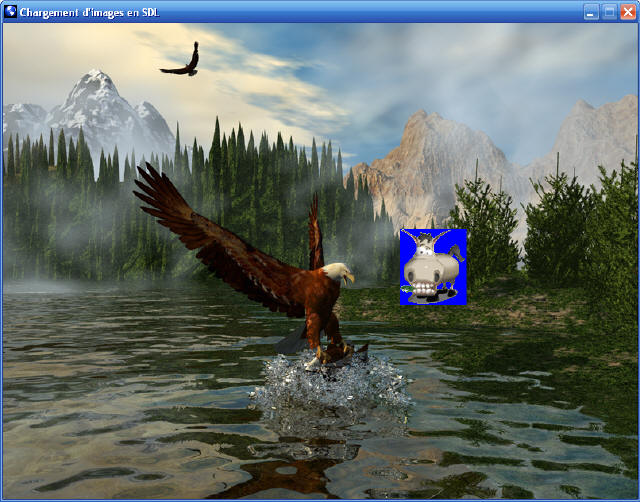
\includegraphics[width=0.8\textwidth]{Chapter_III-3_Window-Image-Zozor}
\end{figure}

يبدو المشهد سيّئا، أليس كذلك ؟

\begin{question}
بالطبع يعود ذلك إلى الخلفية الزرقاء التي هي خلف 
\textenglish{Zozor} !
\end{question}

لأنك تعتقد أنه بوجود خلفية سوداء أو بنّيّة، ربما سيكون المظهر لائقاً أكثر ؟ لا بالطبع، المشكل هنا هو أنه من اللازم أن يكون شكل الصورة عبارة عن مستطيل، أي أنه إذا قمنا بلصقها على المشهد، سنرى خلفيتها، مما يشوّه المظهر.

من حسن الحظّ أن الـ\textenglish{SDL}
تتحكم في الشفافية !

\subsection{جعل صورة شفافة}

\subsubsection{الخطوة 1 : تحضير الصورة}

كبداية، يجب تحضير الصورة التي نريد تسويتها على المشهد.\\
الصيغة 
\textenglish{BMP}
لا تتحكم في الشفافية، على عكس الصيغتين 
\textenglish{GIF}
و 
\textenglish{PNG}.
لهذا يحب علينا أن نجد حلاً آخر. 

يجب استعمال نفس اللون للخلفية على الصورة. هذه الأخيرة ستكون شفافة من طرف الـ\textenglish{SDL}
في وقت التسوية. لاحظ كيف تبدو الصورة
\InlineCode{zozor.bmp}
من ناحية أقرب :

\begin{figure}[H]
	\centering
	
\includegraphics[width=0.2\textwidth]{Chapter_III-3_Zozor}
\end{figure}


الخلفية الزرقاء إذا مـُختارة. لاحظ أنني اخترت اللون الأزرق بشكل عشوائي، كان بإمكاني استعمال اللون الأحمر أو الأصفر مثلاً. الشيء المهم هو أنه يجب على اللون أن يكون وحيداً و موحّدا. لقد اخترت اللون الأزرق لأنه ليس متواجدا في صورة 
\textenglish{Zozor}
لأنني لو اخترت اللون الأخضر، سأخاطر بجعل العشب الذي يتناوله الحمار (أسفل يسار الصورة) شفافاً. 

استعمل إذا أي برنامج كان 
(\textenglish{Paint}، \textenglish{Photoshop}، \textenglish{The Gimp}، \dots
لكلّ واحد منّا ذوقه) لإعطاء خلفية موحّدة للصورة.

\subsubsection{الخطوة 2 : تحديد اللون الشفاف}

لكي نقوم بتحديد اللون الذي يجب أن تجعله
\textenglish{SDL}
شفافاً، يجب أن نستعمل الدالة 
\InlineCode{SDL\_SetColorKey}.
يجب استدعاء هذه الدالة قبل تسوية الصورة.\\
هكذا نقوم بتحويل اللون الذي خلف
\textenglish{Zozor}
إلى الشفاف :

\begin{Csource}
SDL_SetColorKey(zozor, SDL_SRCCOLORKEY, SDL_MapRGB(zozor->format, 0, 0, 255));
\end{Csource}

هناك ثلاثة معاملات :

\begin{itemize}
	\item المساحة التي يجب أن نقوم بتحويلها إلى اللون الشفاف (هنا نتكلم عن 
	\InlineCode{zozor}).
	\item قائمة الأعلام : استعمل 
	\InlineCode{SDL\_SRCCOLORKEY}
	لتفعيل الشفافية، 0 من أجل تعطيلها.
	\item حدد بعد ذلك اللون الذي يجب أن يتم تحويله إلى الشفاف. لقد استعملت
	\InlineCode{SDL\_MapRGB}
	لإنشاء اللون بصيغة عدد
	(\InlineCode{Uint32})
	كما فعلنا بالسابق. كما ترى إنه اللون الأزرق 
	($0, 0, 255$)
	 الّذي سيتم تحويله إلى الشفاف.
	
\end{itemize}

كملخص، نقوم أولا بتحميل الصورة باستعمال
\InlineCode{SDL\_LoadBMP}،
ثمّ نحدد اللون الشفاف باستعمال
\InlineCode{SDL\_SetColorKey}
ثم نقوم بتسوية المساحة باستعمال
\InlineCode{SDL\_BlitSurface}.

\begin{Csource}
zozor = SDL_LoadBMP("zozor.bmp");
SDL_SetColorKey(zozor, SDL_SRCCOLORKEY, SDL_MapRGB(zozor->format, 0, 0, 255));
SDL_BlitSurface(zozor, NULL, screen, &zozorPosition);
\end{Csource}

النتيجة : تم دمج صورة
\textenglish{Zozor}
بشكل ممتاز في المشهد :

\begin{figure}[H]
	\centering
	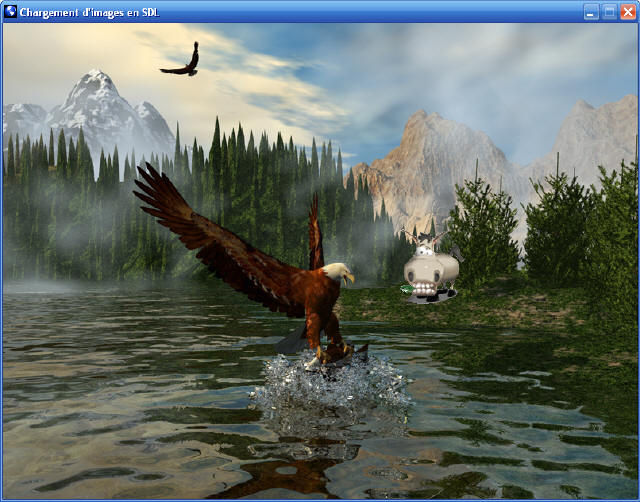
\includegraphics[width=0.8\textwidth]{Chapter_III-3_Window-Image-Zozor-transparent}
\end{figure}

هذه هي التقنية المبدئية التي ستعيد استعمالها كل الوقت في برامجك. تعلّم كيف تتحكم جيداً بالشفافية لأنها من أساسيات صنع لعبة تملك الحدّ الأدنى من الواقعية.

\subsection{الشفافية \textenglish{Alpha}}

هو نوع آخر من الشفافية.\\
لحدّ الآن قمنا بتعريف لون 
\underline{واحد}
شفاف (الأزرق مثلا). هذا اللون لا يظهر في الصورة المُلصقة. 

الشفافية 
\textenglish{Alpha}
توافق شيئاً آخر، إنها تسمح بعمل "مزج" بين صورة و خلفية. هذا نوع من التلاشي.

يمكن تفعيل الشفافية
\textenglish{Alpha}
لمساحة عن طريق الدالة
\InlineCode{SDL\_SetAlpha} :

\begin{Csource}
SDL_SetAlpha(zozor, SDL_SRCALPHA, 128);
\end{Csource}

يوجد هنا ثلاثة معاملات كذلك :

\begin{itemize}
	\item المساحة التي نتكلم عنها (\InlineCode{zozor}).
	\item قائمة الأعلام : ضع
	\InlineCode{SDL\_SRCALPHA}
من أجل تفعيل الشفافية، 0 من أجل تعطيلها.
	\item مهم جدا : قيمة الشفافية 
\textenglish{Alpha}
هي عدد يتراوح بين 0 (صورة شفافة تماماً أي غير مرئية) و 255 (صورة ظاهرة كلياً، و كأن الشفافية
\textenglish{Alpha}
لم تكن موجودة).
\end{itemize}

كلما كان العدد
\textenglish{Alpha}
صغيراً كلما زادت شفافية الصورة و تلاشيها في الخلفية.

هذا مثال عن شفرة تقوم بتطبيق شفافية بقيمة 128 على الصورة
\textenglish{Zozor} :

\begin{Csource}
zozor = SDL_LoadBMP("zozor.bmp");
SDL_SetColorKey(zozor, SDL_SRCCOLORKEY, SDL_MapRGB(zozor->format, 0, 0, 255));
/* Average Alpha transparency (128) : */
SDL_SetAlpha(zozor, SDL_SRCALPHA, 128);
SDL_BlitSurface(zozor, NULL, screen, &zozorPosition);
\end{Csource}

تلاحظ أنني حافظت على شفافية 
\InlineCode{SDL\_SetColorKey}.
يمكن دمج النوعين الاثنين للشفافية معاً.

الجدول التالي يوضّح لك كيف يبدو
\textenglish{Zozor}
باختلاف قيم
\textenglish{Alpha}.

\begin{Table}{2}
\textenglish{Alpha} & النتيجة\\
255 (مرئيّة بالكامل) &
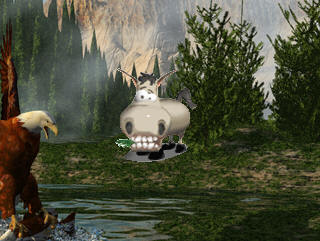
\includegraphics[width=0.25\textwidth]{Chapter_III-3_Window-Image-Zozor-Alpha-255} \\
190 &
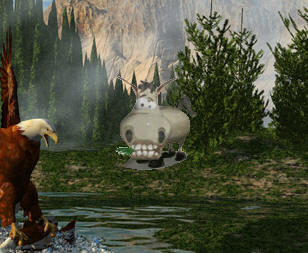
\includegraphics[width=0.25\textwidth]{Chapter_III-3_Window-Image-Zozor-Alpha-190} \\
128 (شفافيّة متوسّطة) &
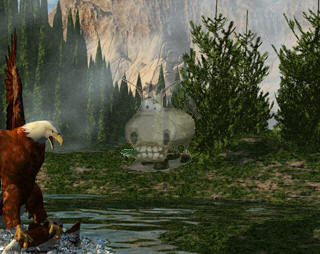
\includegraphics[width=0.25\textwidth]{Chapter_III-3_Window-Image-Zozor-Alpha-128} \\
75 &
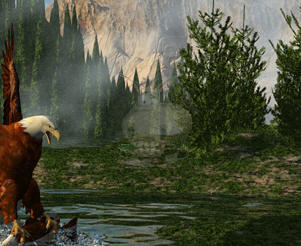
\includegraphics[width=0.25\textwidth]{Chapter_III-3_Window-Image-Zozor-Alpha-75} \\
\end{Table}
\begin{Table*}{2}
0 (غير مرئيّة بالكامل) &
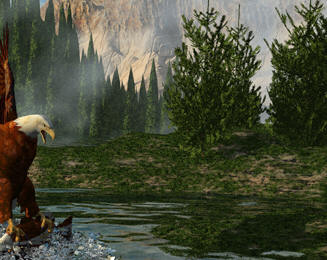
\includegraphics[width=0.25\textwidth]{Chapter_III-3_Window-Image-Zozor-Alpha-0} \\
\end{Table*}


\begin{information}
قيمة الشفافية
\textenglish{Alpha}
128 (شفافية متوسطة) هي قيمة خاصّة و كثيرة الإستعمال بالـ\textenglish{SDL}.
هذا النمط من الشفافية أسرع من ناحية حسابات المعالج مقارنة بالأنماط الأخرى. قد يكون من المهم لك معرفة هذه المعلومة خاصة إن كنت تستعمل الشفافية
\textenglish{Alpha}
بشكل كبير في برامجك.
\end{information}

\section{تحميل صيغ صور أخرى باستعمال الـ\textenglish{SDL\_Image}}

الـ\textenglish{SDL}
لا تتعامل إلا مع الـ\textenglish{bitmap}
(الصيغة
\textenglish{BMP})
كما رأينا.\\
و لكن هذا ليس بمشكل لأن قراءة الصور ذات الصيغة 
\textenglish{BMP}
أسرع بالنسبة للـ\textenglish{SDL}،
و لكن يجب معرفة أنه في أيامنا هذه يتم استعمال صيغ أخرى للصور. بالتحديد الصيغ "المضغوطة" كالـ\textenglish{PNG}،
الـ\textenglish{GIF}
و الـ\textenglish{JPEG}.
لهذا الغرض توجد مكتبة تسمى
\textenglish{SDL\_Image}
و تقوم بالتعامل مع كل صيغ الصور التالية :

\begin{itemize}
	\item \textenglish{TGA}،
	\item \textenglish{BMP}،
	\item \textenglish{PNM}،
	\item \textenglish{XPM}،
	\item \textenglish{XCF}،
	\item \textenglish{PCX}،
	\item \textenglish{GIF}،
	\item \textenglish{JPG}،
	\item \textenglish{TIF}،
	\item \textenglish{LBM}،
	\item \textenglish{PNG}.
\end{itemize}

بالمناسبة فإنه بالإمكان أن تتم إضافة صيغ أخرى للـ\textenglish{SDL}.
و هي المكتبات التي تحتاج إلى الـ\textenglish{SDL}
لكي تعمل. يمكننا تسمية هذا الأمر بالـ\textenglish{add-ons}
(بمعنى "إضافات").
\textenglish{SDL\_Image}
هي واحدة من بين هذه المكتبات.

\subsection{تثبيت الـ\textenglish{SDL\_Image} على \textenglish{Windows}}

\subsubsection{التنزيل}

توجد صفحة خاصة من موقع الـ\textenglish{SDL}
تشير إلى المكتبات التي تستعملها الـ\textenglish{SDL}.
هذه الصفحة تحمل عنوان
"\textenglish{Libraries}".
ستجد رابطاً في القائمة اليسارية.\\
ستلاحظ أن هناك الكثير من المكتبات و أغلبها ليس من طرف المبرمجين الأصليين للـ\textenglish{SDL}.
بل هم مبرمجون عاديون يستعملون الـ\textenglish{SDL}
و يقومون باقتراح مكتباتهم الخاصة لتحسين هذه الأخيرة.

بعض هذه المكتبات مفيد جداً و يستحق إلقاء النظر عليه، و بعضها أقلّ جودة بل ربّما فيه أخطاء. لهذا يجب ترتيب هذه المكتبات حسب أهميتها.

حاول إيجاد
\textenglish{SDL\_Image}
في القائمة، ستدخل إلى الصفحة المخصصة لهذه المكتبة :

\url{https://www.libsdl.org/projects/SDL_image}

نزّل النسخة التي تناسبك من القسم
"\textenglish{Binary}"
(لا تحمّل الملفات المصدرية، لن نحتاجها !).\\
إذا كنت تعمل على
\textenglish{Windows}،
نزّل الملف
\InlineCode{SDL\_image-devel-1.2.10-VC.zip}،
و هذا حتى و إن لم تكن تستعمل البيئة التطويرية 
\textenglish{Visual C++} !

\subsubsection{التثبيت}

في الملف
\InlineCode{.zip}
هذا، ستجد :

\begin{itemize}
	\item \InlineCode{SDL\_image.h} :
	 الملف الرأسي الوحيد الذي تحتاجه الـ\textenglish{SDL\_Image}،
	 قم بلصقه في المسار
	 
	 \InlineCode{C:\textbackslash Program Files\textbackslash CodeBlocks\textbackslash SDL-1.2.13\textbackslash include}
	 
	 بمعنى آخر، إلى جانب الملفات الرأسية للـ\textenglish{SDL}.
	\item \InlineCode{SDL\_image.lib} :
	قم بلصقه في المسار
	
	\InlineCode{C:\textbackslash Program Files\textbackslash CodeBlocks\textbackslash SDL-1.2.13\textbackslash lib}.
	
	أعرف أنك ستخبرني بأن الملفات ذات الامتداد
	\InlineCode{.lib}
	هي محجوزة للبيئة التطويرية
	\textenglish{Visual C++}،
	لكن هذه حالة استثنائية، فالملف 
	\InlineCode{.lib}
	يعمل حتى مع المترجم 
	\textenglish{mingw}.
	\item الكثير من الملفات
	\textenglish{DLL} : 
	قم بوضعها كلها في المجلّد الخاص بالمشروع (أي بجانب الملف 
	\InlineCode{SDL.dll}).
\end{itemize}

بعد ذلك، يجدر بك تغيير خواص المشروع من أجل محرّر الروابط
(\textenglish{Linker})
للملف
\InlineCode{SDL\_image.lib}.

إذا كنت تعمل بالـ\textenglish{Code::Blocks}
مثلاً، توجّه إلى القائمة
\InlineCode{Projects} / \InlineCode{Build options}،
في الفرع
\InlineCode{Linker}
أنقر على الزر 
\InlineCode{Add}
و اختر المسار الذي يتواجد به الملف
\InlineCode{SDL\_image.lib}،
لاحظ الصورة :

\begin{figure}[H]
	\centering
	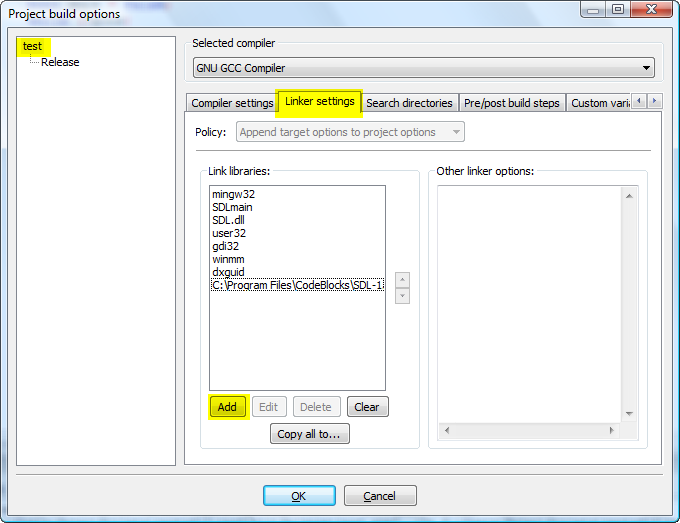
\includegraphics[width=0.8\textwidth]{Chapter_III-3_CodeBlocks-Linker}
\end{figure}

إذا ظهرت لك رسالة تحمل سؤال : 
"\textit{\textenglish{Keep as a relative path ?}}"،
فلتجب بما أردت لأنه لن يغير شيئاً في الوقت الحالي. أنصحك بالإجابة بالسلب، شخصيّا.

بعد ذلك، ما عليك سوى تضمين الملف الرأسي
\InlineCode{SDL\_image.h}
في الشفرة المصدرية. على حسب المكان الذي وضعت فيه الملف
\InlineCode{SDL\_image.h}
سيكون عليك استعمال هذه الشفرة :

\begin{Csource}
#include <SDL/SDL_image.h>
\end{Csource}

أو هذه

\begin{Csource}
#include <SDL_image.h>
\end{Csource}

جرّبهما كليهما، يجدر بأحداهما أن تعمل.

\begin{information}
إذا كنت تعمل بالـ\textenglish{Visual Studio}
فستكون العمليّة نفسها. لأنه إن تمكنت من تثبيت الـ\textenglish{SDL}
لن يصعب عليك تثبيت الـ\textenglish{SDL\_Image}.
\end{information}

\subsection{تثبيت الـ\textenglish{SDL\_Image} على \textenglish{Mac OS X}}


إن كنت تستعمل
\textenglish{Mac OS X}،
نزّل الملف ذا الامتداد
\InlineCode{.dmg}
من موقع الـ\textenglish{SDL}
و ضعه في المجلد\\
\InlineCode{Library/Frameworks}.

اكتب بعد ذلك
"\textenglish{search paths}"
 في حقل البحث الخاص بـ\textenglish{Xcode}.
 اعثر على السطر\\
\InlineCode{Header search paths}،
 انقر مرتين على السطر من اليمين و أضف\\
\InlineCode{/Library/Frameworks/SDL\_image.framework/Headers}.

لم يبق لك سوى إضافة إطار العمل إلى المشروع. الصورة التالية توضح لك كيف يظهر\\
الـ\InlineCode{Header search paths}
بعد تثبيت الـ\textenglish{SDL\_image}.

\begin{figure}[H]
	\centering
	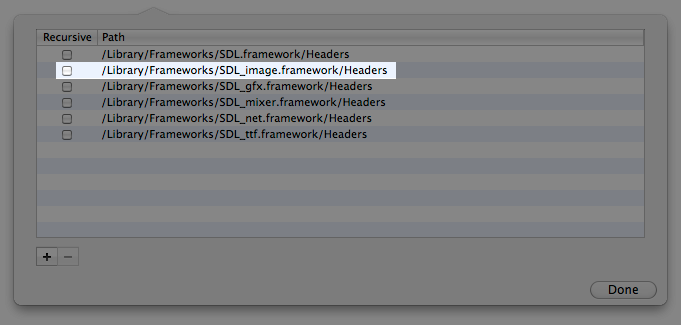
\includegraphics[width=\textwidth]{Chapter_III-3_Xcode-frameworks}
\end{figure}

و بهذا يجب عليك تضمين الملف الرأسي في بداية الكود كالتالي :
\begin{Csource}
#include "SDL_image.h"
\end{Csource}
في عوض استعمال الإشارتين
\InlineCode{< >}
 قم باستعمال الكتابة السابقة فيما سأعطيك لاحقا.

\subsection{تحميل الصور}

الحقيقة أن تثبيت الـ\textenglish{SDL\_image}
أصعب بمئة مرة من استعمالها ! إنه عليك أنت تحديد صعوبة العمل بالمكتبة~! 

توجد دالة وحيدة عليك معرفتها : 
\InlineCode{IMG\_Load}.\\
و هي تستقبل معاملا واحدا : اسم الملف الذي نريد فتحه.

و هذا أمر عملي لأن هذه الدالة تتمكن من تحميل أي نوع من الملفات التي تتعامل معهاالـ\textenglish{SDL\_image}
(\textenglish{JPG}، \textenglish{PNG}، \textenglish{GIF}
و حتى الـ\textenglish{TIF}،
إلخ). إذ تقوم وحدها بتحديد نوع الملف من خلال امتداده.
\begin{question}
بما أن الـ\textenglish{SDL\_Image}
تستطيع أيضاً فتح الصور 
\textenglish{BMP}،
فيمكنك الآن نسيان أمر استعمال الدالة 
\InlineCode{SDL\_LoadBMP}
و استعمال الدالة 
\InlineCode{IMG\_Load}
لتحميل كل أنواع الصور.
\end{question}

شيء جيد آخر : إذا كانت الصورة التي تحمّلها تملك الشفافية (كما هو حال الصور 
\textenglish{PNG}
و
\textenglish{GIF})
 فإنّ
\textenglish{SDL\_Image}
تفعّل تلقائيّا الشفافية من أجل هذه الصورة ! مما يعني عدم وجود داعٍ لاستدعاء الدالة 
\InlineCode{SDL\_SetColorKey}.

سأٌقدّم لك الشفرة المصدرية التي تقوم بتحميل الصورة 
\InlineCode{sapin.png}
و إظهارها.\\
لاحظ جيدا أنني قمت بتضمين
\InlineCode{SDL/SDL\_image.h}
كما أنني لا استدعي الدالة 
\InlineCode{SDL\_SetColorKey}
لأن الصورة
\textenglish{PNG}
التي استعملها شفافة طبيعيّا.\\
سترى أنني أستعمل الدالة 
\InlineCode{IMG\_Load}
في كلّ مكان بالشفرة و ذلك بتعويض الدالة 
\InlineCode{SDL\_LoadBMP}.

\begin{Csource}
#include <stdlib.h>
#include <stdio.h>
#include <SDL/SDL.h>
/* including the header of SDL_image (adapt to your directory) */
#include <SDL/SDL_image.h> 
void pause();
int main(int argc, char *argv[])
{
	SDL_Surface *screen = NULL, *backgoundImage = NULL, *sapin = NULL;
	SDL_Rect backgoundPosition, sapinPosition;
	backgoundPosition.x = 0;
	backgoundPosition.y = 0;
	sapinPosition.x = 500;
	sapinPosition.y = 260;
	SDL_Init(SDL_INIT_VIDEO);
	SDL_WM_SetIcon(IMG_Load("sdl_icone.bmp"), NULL);
	screen = SDL_SetVideoMode(800, 600, 32, SDL_HWSURFACE);
	SDL_WM_SetCaption("Loading images on SDL", NULL);
	backgoundImage = IMG_Load("lac_en_montagne.bmp");
	SDL_BlitSurface(backgoundImage, NULL, screen, &backgoundPosition);
	/* Loading a PNG image with IMG_Load
	We won't have any problem because the PNG image contains the transparency information inside */
	sapin = IMG_Load("sapin.png");
	SDL_BlitSurface(sapin, NULL, screen, &sapinPosition); 
	SDL_Flip(screen);
	pause();
	SDL_FreeSurface(backgroundImage);
	SDL_FreeSurface(sapin);
	SDL_Quit();
	return EXIT_SUCCESS;
} 
void pause()
{
	int cont = 1;
	SDL_Event event;
	while (cont)
	{
		SDL_WaitEvent(&event);
		switch(event.type)
		{
			case SDL_QUIT:
			cont = 0;
		}
	}
}
\end{Csource}

كما يمكننا الملاحظة، فقد تم دمج الصورة مع الخلفية بشكل ممتاز :

\begin{figure}[H]
	\centering
	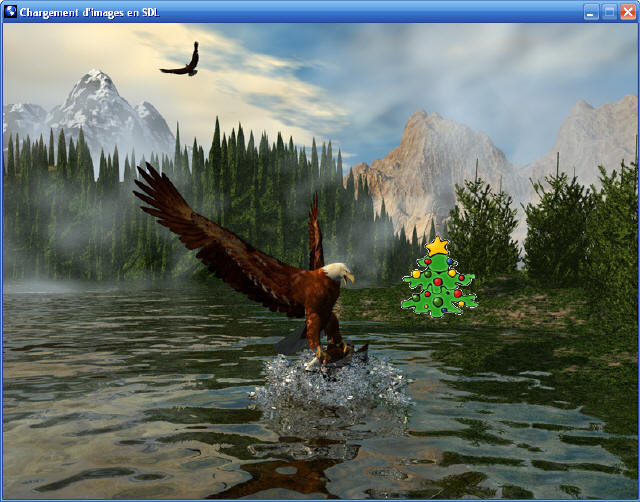
\includegraphics[width=0.8\textwidth]{Chapter_III-3_Window-Image-Sapin}
\end{figure}

\section*{ملخّص}

\begin{itemize}
	\item تسمح الـ\textenglish{SDL}
	بتحميل صور على مساحات. افتراضيّا، هي تسمح بالتعامل مع الصور ذات الصيغة
	\textenglish{BMP}
	باستعمال الدالة
	\InlineCode{SDL\_LoadBMP}.
	\item يمكننا تعريف لون شفاف باستعمال الدالة
	\InlineCode{SDL\_SetColorKey}.
	\item يمكننا جعل الصورة أكثر أو أقل شفافية و ذلك باستعمال الدالة 
	\InlineCode{SDL\_SetAlpha}.
	\item المكتبة
	\textenglish{SDL\_image}
	تسمح بإدخال صور من أيّة صيغة كانت
	(\textenglish{JPG}، \textenglish{PNG}، \dots)
	باستعمال الدالة
	\InlineCode{IMG\_Load}.
	لكن علينا تسطيب هذه المكتبة بالإضافة إلى الـ\textenglish{SDL}.
\end{itemize}

  \chapter{معالجة الأحداث (\textenglish{Event handling})}

معالجة الأحداث هو من أهم الأساسيات في الـ\textenglish{SDL}.\\
و ربّما قد يكون الشطر الأكثر شغفاً لاكتشافه. لأنه انطلاقا من هنا ستبدأ فعلاً في التحكّم في تطبيقك.

كلّ من مرفقات الحاسوب (فأرة، لوحة مفاتيح، \dots) قادرة على إنتاج حدث. سنتعلّم كيف نستقبل كل حدث و نتعامل معه. تطبيقك سيصبح أخيراً تفاعليّا !

فعلياً، ما هو الحدث ؟ الحدث هو عبارة عن إشارة
(\textenglish{signal})
يتم إرسالها عن طريق إحدى مرفقات الحاسوب 
(\textenglish{peripherals})
(أو عن طريق نظام التشغيل بذاته) إلى التطبيق. هذه أمثلة عن بعض الأحداث المألوفة :

\begin{itemize}
	\item حينما يضغط المُستعمل على زر من لوحة المفاتيح.
	\item و أيضاً حينما ينقر بالفأرة.
	\item حينما يحرّك الفأرة.
	\item حينما يقوم بتصغير النافذة.
	\item حينما يطلب إغلاق النافذة.
	\item إلى آخره.
\end{itemize}

الهدف من هذا الفصل هو تعلّم كيفية معالجة الأحداث. يمكنك أخيراً القول للحاسوب : "إذا نقر المستعمل في هذا المكان، قم بفعل كذا، و إن لم يفعل، قم بكذا. إذا حرّك الفأرة، قم بكذا. إذا ضغط على الزر
\InlineCode{Q}،
أوقف البرنامج. إلخ".

\section{مبدأ عمل الأحداث}

لنتعوّد على الأحداث، سنتعلّم كيف نتعامل مع أسهل حدث :
\textbf{طلب غلق البرنامج}.
هذا حدث يـُنتجُ حينما يقوم المستعمل بالنقر على الزر
\InlineCode{X} :

\begin{figure}[H]
	\centering
	
\includegraphics[width=0.05\textwidth]{Chapter_III-4_Close}
\end{figure}

إنه فعلاً الحدث الأكثر سهولة. إضافة على ذلك، هو حدث قد استعملته سابقاً دون أن تعلم بذلك لأنه متواجد في الدالة 
\InlineCode{pause} !\\
بالفعل، دور هذه الدالة هو انتظار المستعمل حتّى يقررّ غلق البرنامج، لأننا لو لم نستعملها كانت النافذة لتظهر و تختفي بسرعة البرق !

\begin{information}
يمكنك من الآن نسيان الدالة
\InlineCode{pause}.
قم بحذفها من الشفرة المصدرية لأننا سنتعلّم كيف نكتب محتواها بأنفسنا.
\end{information}

\subsection{متغيّر الحدث}

لمعالجة الأحداث، ستحتاج إلى التصريح عن متغيّر (واحد فقط، كن متأكدا) من نوع 
\InlineCode{SDL\_Event}.\\
فلتقم بتسميته بالاسم الذي يحلو لك، أنا سأسمّيه 
\InlineCode{event}،
و هي تعني "حدث" بالإنجليزيّة.

\begin{Csource}
SDL_Event event;
\end{Csource}

من أجل اختبارات الشفرة، سنستعمل دالة
\InlineCode{main}
بسيطة للغاية تقوم بإظهار نافذة فقط، مثلما رأينا في الفصول الأولى. هذا ما يجب أن تبدو عليه الدالة
\InlineCode{main} :

\begin{Csource}
int main(int argc, char *argv[])
{
	SDL_Surface *screen = NULL;
	SDL_Event event; // This variable will help us to manage the events
	SDL_Init(SDL_INIT_VIDEO);
	screen = SDL_SetVideoMode(640, 480, 32, SDL_HWSURFACE);
	SDL_WM_SetCaption("Managing the events in SDL", NULL);
	SDL_Quit();
	return EXIT_SUCCESS;
}
\end{Csource}

إذا، هي شفرة بدائية جداً، و هي لا تحوي سوى شيء جديد : تعريف المتغير
\InlineCode{event}
الذي سنستعين به قريباً.

جرّب الشفرة : مثلما توقّعنا، يجدر بالنافذة أن تظهر و تختفي في لحظة.

\subsection{حلقة الأحداث}

حينما نريد انتظار حدث، نستعمل غالباً حلقة. هذه الحلقة التكرارية تستمر في الاشتغال مادُمنا لم نستقبل الحدث المـُراد.\\
يجب علينا أن نستعمل متغيراً منطقياً لكي يحدد لنا ما إن كان علينا البقاء في الحلقة أو الخروج منها.\\
أنشئ هذا المتغير و سمّه مثلا
\InlineCode{cont}\footnote{
إذا كنت تفكّر في تسميته
\InlineCode{continue}
فلا تفعل، لأنّها كلمة مفتاحيّة (محجوزة)، و بالتالي لا يمكن استخدامها كاسم لمتغيّر.} :

\begin{Csource}
int cont = 1;
\end{Csource}

هذا المتغير المنطقي يأخذ القيمة 1 في البداية لأننا نريد للحلقة أن تتكرر مادام المتغير
\InlineCode{cont}
يحمل هذه القيمة (صحيح). ما إن يأخذ المتغير المنطقي القيمة 0 (خطأ)، نخرج من الحلقة و يتوقف البرنامج.

هذا ما تبدو عليه الحلقة :

\begin{Csource}
while (cont)
{
	// Dealing with the event
}
\end{Csource}

هكذا إذاً : لدينا لحدّ الآن حلقة غير منتهية لا تنتهي إلا إذا أخذ المتغير 
\InlineCode{cont}
القيمة 0. الأكثر أهمية هو ما نكتبه في داخل تلك الحلقة.

\subsection{استرجاع الحدث}

الآن سنقوم باستدعاء دالة من الـ\textenglish{SDL}
لكي نتحقق ما إن تم إنتاج حدث.\\
لدينا دالتان للقيام بهذا العمل، لكن كلا منهُما تعمل بطريقة مختلفة عن الأخرى :

\begin{itemize}
	\item \InlineCode{SDL\_WaitEvent} :
	تقوم بانتظار إنتاج حدث. هذه الدالة نقول عنها تعطيلية لأنها توقف عمل البرنامج مادام لم يتم إنتاج أي حدث.
	\item \InlineCode{SDL\_PollEvent} :
	هذه الدالة تقوم بنفس العمل لكنها ليست تعطيلية. لأنها تُخبرنا ما إن تم إنتاج حدث أم لا، فإن لم يكن هناك أي حدث فإنها تعيد التحكّم إلى البرنامج مباشرة.
\end{itemize}

هاتان الدالّتان مهمّتان، لكن في حالتين مختلفتين.\\
لتبسيط الأمور، إذا استعملت 
\InlineCode{SDL\_WaitEvent}
فإن برنامجك لن يـُتعب كثيراً المـُعالج لأنه سيتوقف مـُنتظراً إنتاج حدث.\\
بالمـُقابل، إذا استعملت 
\InlineCode{SDL\_PollEvent}،
سيقوم البرنامج بالعمل على الحلقة
\InlineCode{while}
و استدعاء الدالة 
\InlineCode{SDL\_PollEvent}
بشكل غير معرّف إلى حين إنتاج حدث مُعين. و بهذا تستعمل المُعالج  بنسبة 100
\%.

\begin{question}
لكن ألا يجب أن نستعمل دائماً الدالة 
\InlineCode{SDL\_WaitEvent}
بما أنها لا تستعمل المـُعالج كثيراً ؟
\end{question}

كلّا، لأنه توجد حالات لا يمكن الاستغناء فيها عن الدالة 
\InlineCode{SDL\_PollEvent}.
و هي حالة الألعاب التي يتم فيها تحديث الشاشة حتى و إن لم يكن هناك أي حدث.\\
فلنأخذ مثلاً اللعبة 
\textenglish{Tetris} :
تقوم الكتل بالنزول لوحدها، لا يحتاج المُستعمل إلى إنتاج حدث من أجل حصول هذا الأمر ! لو استعملنا
\InlineCode{SDL\_WaitEvent}،
سيبقى البرنامج مـُعطّلا و لن تتمكّن من تحديث الشاشة لإنزال الكتل !

\begin{question}
ماذا تفعل
\InlineCode{SDL\_WaitEvent}
لكي لا تستهلك من الـمُعالج كثيراً ؟\\
فبعد كل شيء، الدالة مُجبرة على البقاء في حلقة غير منتهية لكي تختبر كلّ الوقت ما إن كان هناك حدث أم لا، أليس كذلك ؟
\end{question}

الحقيقة أنني كنت أطرح هذا السؤال قبل وقت قليل. الإجابة معقّدة قليلاً لأنها تخصّ الطريقة التي يتحكّم فيها النظام بالعمليّات 
(\textenglish{Processes})
(البرامج التي هي في طور الاشتغال).\\
إذا كنت تريد -لكنّي سأتحدّث بسرعة-، بالنسبة للدالة 
\InlineCode{SDL\_WaitEvent}،
عمليّة البرنامج تُوضع في طور الانتظار.\\
إذا فإن البرنامج لا يعمل عليه المعالج بعد تلك اللحظة.\\
سيتم "إيقاظه" من طرف نظام التشغيل حينما يتم إنتاج حدث. يعني أن المعالج سيعود إلى العمل على البرنامج في هذه اللحظة. هذا ما يشرح لِمَا لا يستهلك البرنامج من المعالج شيئا بينما يكون في طور انتظار الحدث.

أدري أن هذه المفاهيم تبدو مجرّدة لك الآن. لكنك لست مُجبراً على فهم كل هذا الآن لأنك ستبدأ في التأقلم مع هذه المعلومات شيئاً في شيئاً مع التطبيق.\\
الآن سنستعمل 
\InlineCode{SDL\_WaitEvent}
لأن البرنامج سيبقى بسيطا باستخدامها. على أي حال فالتعامل مع هاتين الدالتين لن يتغير من واحدة إلى أخرى.

يجب أن تبعث للدالة عنوان المتغير 
\InlineCode{event}
الذي يقوم بتخزين الحدث.\\
بما أن هذا المتغير ليس عبارة عن مؤشّر (أعد رؤية طريقة التصريح به أعلاه)، سنستعمل الاشارة
\InlineCode{\&}
قبل اسم المتغير و ذلك لنُعطي عنوانه :

\begin{Csource}
SDL_WaitEvent(&event);
\end{Csource}

بعد استدعاء هذه الدالة، المتغير
\InlineCode{event}
يحتوي إجبارياً حدثاً ما.

\begin{information}
هذه الحالة ليست نفسها لو استعملنا
\InlineCode{SDL\_PollEvent}
لأن هذه الأخيرة قادرة على أن تُرجع لنا : "لا يوجد أي حدث".
\end{information}

\subsection{تحليل الحدث}

الآن نحن نتوفر على متغير
\InlineCode{event}
يحتوي على معلومات حول الحدث الذي تم إنتاجه.\\
يجب أن نرى المركّب
\InlineCode{event.type}
و نختبر قيمته. غالبا ما نستعمل
\InlineCode{switch}
لاختبار الحدث.

\begin{question}
لكن كيف لنا أن نعرف ما هي القيمة الموافقة للحدث "أغلق البرنامج" مثلا ؟
\end{question}

الـ\textenglish{SDL}
توفّر لنا بعض الثوابت، مما يسهّل كثيراً كتابة البرنامج. هذه الثوابت كثيرة العدد (بقدر وجود أحداث ممكن حصولها في الحاسوب). سنتعرّف على هذه الثوابت بتقدّمنا في هذا الفصل.

\begin{Csource}
while (cont)
{
	SDL_WaitEvent(&event); // Getting the event in "event"
	switch(event.type) // Testing the event's type
	{
		case SDL_QUIT: // If it's a quit event
		cont = 0;
		break;
	}
}
\end{Csource}

هكذا تعمل الشفرة :

\begin{enumerate}
	\item ما إن يتم انتاج حدث، تُرجع الدالة 
	\InlineCode{SDL\_WaitEvent}
	الحدث في المتغير 
	\InlineCode{event}.
	\item نقوم بتحليل نوع الحدث بالاستعانة بـ\InlineCode{switch}.
	نوع الحدث موجود في
	\InlineCode{event.type}.
	\item نختبر بمساعدة 
	\InlineCode{case}
	نوع الحدث. لحدّ الآن، نحن لا نتحقق إلا إذا ما كان الحدث يوافق
	\InlineCode{SDL\_QUIT}
	(طلب إغلاق البرنامج)، لأنّها الحالة الوحيدة التي تهمّنا.
	\item إذا كان الحدث هو 
	\InlineCode{SDL\_QUIT}،
	فهذا يعني أن المستعمل طلب إغلاق البرنامج. في هذه الحالة، نعطي للمتغير المنطقي
	\InlineCode{cont}
	القيمة 0. في الدورة القادمة للحلقة، سيكون الشرط غير محقق، فيتوقف تشغيل البرنامج.
	\item إذا لم يكن الحدث هو 
	\InlineCode{SDL\_QUIT}،
	مما يعني أنه قد حدث شيء آخر : قام المستعمل بالضغط على زر، بالنقر على الفأرة أو ببساطة قام بتحريك الفأرة داخل النافذة. و بما أن هذه الأحداث لا تهمّنا، لن نقوم بمعالجتها. لن نقوم إذا بأي شيء : تقوم الحلقة بالانتقال في كلّ مرة إلى دورة جديدة ننتظر فيها وقوع حدث جديد (بمعنى آخر، نعود إلى النقطة 1).
\end{enumerate}

ما أنا أشرحه لك الآن هو أمر مهم جداً. إذا فهمت هذه الشفرة، فقد فهمت كلّ شيء و سيكون باقي الفصل سهلاً للغاية.

\subsection{الشفرة الكاملة}

\begin{Csource}
int main(int argc, char *argv[])
{
	SDL_Surface *screen = NULL;
	SDL_Event event; // The event's variable
	int cont = 1; // A boolean for the loop
	SDL_Init(SDL_INIT_VIDEO);
	screen = SDL_SetVideoMode(640, 480, 32, SDL_HWSURFACE);
	SDL_WM_SetCaption("Managing the events in SDL", NULL);
	while (cont) // While the variable's value is 
	{            // not equal to 0
		SDL_WaitEvent(&event); // We wait for an event that we recuperate in "event"
		switch(event.type) // Testing the event's type
		{
			case SDL_QUIT: // If it's a quit event
			cont = 0; // We change the boolean value so we go out from the loop.
			break;
		}
	}
	SDL_Quit();
	return EXIT_SUCCESS;
}
\end{Csource}

هاهي الشفرة الكاملة. لا يوجد شيء صعب : إذا قمت بمتابعة الفصل إلى الآن، يجدر بك أن تكون قد فهمت كلّ شيء. على أي حال فقد لاحظت أنّنا لم نقم إلا بإعادة كتابة ما تقوم به الدالة 
\InlineCode{pause}.
قارن هذه الشفرة بما تقوم به الدالة
\InlineCode{pause} :
هو نفس الشيء، إلا أنه في هذه الحالة نقوم بوضع كلّ شيء في الدالة
\InlineCode{main}.
بالطبع، من المستحسن نقل الشفرة إلى دالة أخرى على حدى كـ\InlineCode{pause}،
لأن ذلك سيقلّل من حجم الدالة
\InlineCode{main}
و يجعلها أفضل من ناحية فهم الشفرة.

\section{لوحة المفاتيح}

سنقوم الآن بدراسة الأحداث التي تـُنتج عن طريق لوحة المفاتيح.

إذا فهمت بداية الفصل، فلن تواجه أي مشكل في التعامل مع أي نوع من الأحداث. لا يوجد ماهو أسهل.

لماذا هذا سهل ؟ لأننا الآن فهمنا طريقة عمل الحلقة التكرارية غير المنتهية، كل ما ستقوم بفعله هو إضافة بعض الحالات إلى الـ\InlineCode{switch}
من أجل تحليل أنواع أخرى من الأحداث. لا يفترض أن يكون هذا الأمر صعباً.

\subsection{أحداث لوحة المفاتيح}

يوجد نوعان من الأحداث التي يمكن توليدها عن طريق لوحة المفاتيح :

\begin{itemize}
	\item \InlineCode{SDL\_KEYDOWN} :
حينما يتم بدأ الضغط على زر من لوحة المفاتيح.
	\item \InlineCode{SDL\_KEYUP} :
حينما يتحرر زر لوحة المفاتيح.
\end{itemize}

لماذا يوجد حدثان إثنان ؟\\
لأننا حينما نضغط على زر، يحدث أمران : شدّ الزر إلى الأسفل
(\InlineCode{SDL\_KEYDOWN})
ثمّ تحريره 
(\InlineCode{SDL\_KEYUP}).
تسمح لنا الـ\textenglish{SDL}
بتحليل كل من هذين الحدثين على حدى، و هذا أمر عملي جداً، سترى ذلك.

لحدّ الآن سنكتفي بتحليل الحدث
\InlineCode{SDL\_KEYDOWN}
(الضغط على الزر) :

\begin{Csource}
while (cont)
{
	SDL_WaitEvent(&event);
	switch(event.type)
	{
		case SDL_QUIT:
		cont = 0;
		break;
		case SDL_KEYDOWN: // If we press a button
		cont = 0;
		break;
	}
}
\end{Csource}

إذا ضغطنا على أي زر سيتوقف البرنامج، جرّب ذلك !

\subsection{استرجاع رمز الزر}

معرفة أنه تم الضغط على زر من لوحة المفاتيح هو أمر جيد، لكن معرفة أي الأزرار تم الضغط عليه بالضبط هو أمر أحسن !

يمكننا معرفة الزر الذي تم الضغط عليه بفضل مركّب مركّب مركّب المتغيّر (أوف !) و الذي يُدعى 
\InlineCode{event.key.keysym.sym}.
 هذا المتغير يحتوي قيمة الزر الذي تم الضغط عليه (و هو يعمل حتى في الحين الذي نحرر فيه الزر
\InlineCode{SDL\_KEYUP}).

\begin{information}
الشيء الجيد هو أن الـ\textenglish{SDL}
تسمح باسترجاع هذه القيمة من كل أزرار لوحة المفاتيح و التي تتضمّن على الحروف و الأرقام، و كذلك الأزرار 
\InlineCode{Esc}، \InlineCode{Print scr.}، \InlineCode{Del}، \InlineCode{Enter}، \dots
إلخ.
\end{information}

يوجد ثابت من أجل كل زر في اللوحة. يمكنك الاطلاع على قائمة هذه الثوابت من خلال الملفات التوثيقيّة الخاصة بالـ\textenglish{SDL}،
الّتي من المفترض أنّك قد نزلتها مع المكتبة 
\textenglish{SDL}.\\
إن لم تفعل، فأنصحك بالتوجه إلى موقع المكتبة و تحميل هذه الملفات لأنها مهمّة للغاية.

ستجد قائمة أزرار لوحة المفاتيح في القسم
"\textenglish{Keysym definitions}".
هذه القائمة طويلة جداً و لا يمكنني تقديمها هنا و لهذا عليك تصفح التوثيق من الموقع مباشرة.

\url{http://www.siteduzero.com/uploads/fr/ftp/mateo21/sdlkeysym.html}

هذه الملفات مُحررة باللغة الانجليزية، و هي غير متوفرة بلغة أخرى. إذا كنت تريد البرمجة حقّا، فمن الواجب أن تجيد هذه اللغة لأنّ  كلّ الملفات التوثيقيّة مكتوبة بها، فلا يمكنك أبدا تجاوزها !

يوجد في اللائحة جدولان : واحد كبير (في البداية) و آخر صغير (في النهاية). نحن الآن نهتم بالجدول الأكبر.\\
في العمود الأول تجد الثابت، في العمود الثاني تجد القيمة الموافقة له بالـ\textenglish{ASCII}
و أخيرا في العمود الثالث تجد وصفاً للزر.\\
لاحظ أن بعض الأزرار كـ\InlineCode{Maj}
(\InlineCode{Shift})
لا تملك قيمة
\textenglish{ASCII}
موافقة لها.

فلنأخذ مثلاً الزر
\InlineCode{Esc}.
يمكننا معرفة ما إن كان هذا الزر مضغوطاً كالتالي :

\begin{Csource}
switch (event.key.keysym.sym)
{
	case SDLK_ESCAPE: // Pressing Escape button lets us quit the program
	cont = 0;
	break;
}
\end{Csource}

\begin{information}
أستعمل
\InlineCode{switch}
من أجل الاختبار الأول لكن كان بإمكاني استعمال
\InlineCode{if}
ببساطة.\\
في كلّ مرة أميل إلى الاستعانة بالـ\InlineCode{switch}
حينما أعالج الأحداث لأنني أختبر الكثير من القيم المختلفة (عملياً، يتوفر لدينا الكثير من الحالات في الـ\InlineCode{switch}،
على عكس هذا المثال).
\end{information}

هذه حلقة حدث كاملة يمكنك تجريبها :

\begin{Csource}
while (cont)
{
	SDL_WaitEvent(&event);
	switch(event.type)
	{
		case SDL_QUIT:
		cont = 0;
		break;
		case SDL_KEYDOWN:
		switch (event.key.keysym.sym)
		{
			case SDLK_ESCAPE: 
			cont = 0;
			break;
		}
		break;
	}
}
\end{Csource}

\begin{information}
هذه المرة، يتوقف البرنامج حينما نضغط على الزر
\InlineCode{Esc}
أو إذا نقرنا على الرمز
\InlineCode{X}
أعلى النافذة. و الآن بما أنك تعرف كيف تغلق البرنامج بالضغط على زر معين، أنت مـُخوّل لاستعمال وضع الشاشة الكاملة إذا كان هذا ممتعا لك (استعمل العـَلم
\InlineCode{SDL\_FULLSCREEN}
في الـ\InlineCode{SDL\_SetVideoMode}،
كتذكير).\\
سابقاً كنت قد منعتك من استعمال هذا الأسلوب في العرض خشية أننا لن نتمكن من غلق البرنامج (لأنه لن يظهر لنا زرّ الإغلاق الّذي نضغط عليه لإيقاف البرنامج !)
\end{information}

\section{تمرين : تحريك \textenglish{Zozor} بواسطة لوحة المفاتيح}

أنت الآن قادر على تحريك صورة في النافذة بواسطة لوحة المفاتيح !\\
هذا تمرين مهمّ جداً سيسمح لنا بالتعرف على كيفية استعمال الـ\textenglish{double buffering}
و الاستعمال المتكرر للأزرار.\\
إضافة إلى ذلك، ما أنا بصدد تعليمه لك هو قاعدة كل ألعاب الفيديو التي تُصنع بالـ\textenglish{SDL}.
و لهذا فإن
\textbf{هذا التمرين ليس اختياريا}
! أدعوك لقراءته و محاولة حلّه بشكل جدّي.

\subsection{تحميل الصورة}

في البداية، سنقوم بتحميل صورة. سيكون الأمر بسيطاً : سنعيد استعمال صورة 
\textenglish{Zozor}
المُستعملة في الفصل السابق.\\
أنشئ المساحة
\InlineCode{zozor}،
حمّل الصورة و حوّل خلفيتها إلى اللون الشفاف (أذكرك بأن صيغة الصورة هي 
\textenglish{BMP}).

\begin{Csource}
zozor = SDL_LoadBMP("zozor.bmp");
SDL_SetColorKey(zozor, SDL_SRCCOLORKEY, SDL_MapRGB(zozor->format, 0, 0, 255));
\end{Csource}

بعد ذلك، الشيء الأكثر أهمية، يجب عليك إنشاء متغير من نوع
\InlineCode{SDL\_Rect}
لتقوم بحِفظ مركبات
\textenglish{Zozor}.

\begin{Csource}
SDL_Rect positionZozor;
\end{Csource}

أنصحك بإعطاء قيم ابتدائية للمركبات، ضع مثلا
\InlineCode{x = 0}
و 
\InlineCode{y = 0}
(الوضعية أعلى يسار النافذة) أو قم بـِمـَرْكَـزَة
\textenglish{Zozor}
في وسط النافذة كما قمت بتعليمك هذا من قبل.

\begin{Csource}
// We center Zozor in the screen
zozorPosition.x = screen->w / 2 - zozor->w / 2;
zozorPosition.y = screen->h / 2 - zozor->h / 2;
\end{Csource}

\begin{critical}
يجب عليك تهيئة المتغير 
\InlineCode{zozorPosition}
\textit{بعد}
تحميل المساحتين 
\InlineCode{screen}
و 
\InlineCode{zozor}.
في الواقع، سأستعمل العرض 
\InlineCode{w}
و الارتفاع 
\InlineCode{h}
لهاتين المساحتين من أجل حساب الموقع المركزي لـ\textenglish{Zozor}
في الشاشة، و لهذا كان لازما أن يتم تهيئة هاتين المساحتين من قبل.
\end{critical}

إذا كنت قد تدبّرت أمرك جيّدا، يجدر أن يظهر 
\textenglish{Zozor}
في وسط النافذة.

\begin{figure}[H]
	\centering
	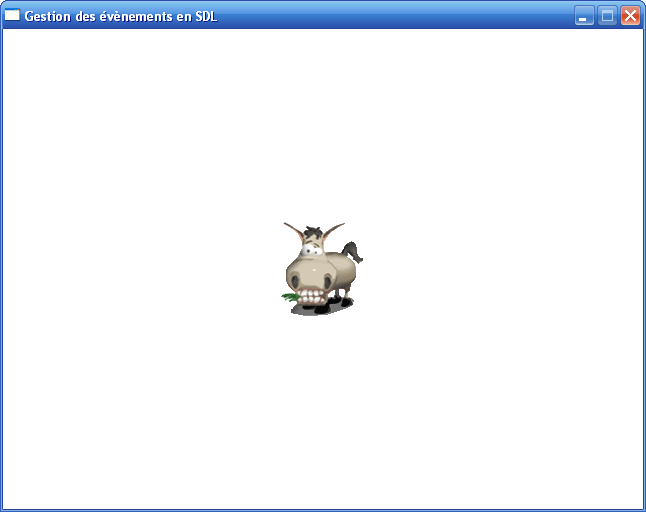
\includegraphics[width=0.8\textwidth]{Chapter_III-4_Window-Zozor}
\end{figure}

لقد اخترت هذه المرة وضع خلفية بيضاء (قمت بـ\InlineCode{SDL\_FillRect})
لكن هذا ليس واجباً.

\subsection{مخطط البرمجة بالأحداث}

حينما تقوم ببرمجة برنامج يتفاعل مع الأحداث (كما سنقوم بفعله الآن)، يجب عليك اتّباع نفس "المخطط" في غالب الأحيان.\\
يجدر بك 
\textit{حفظ هذا المخطط عن ظهر قلب} :

\begin{Csource}
while (cont)
{
	SDL_WaitEvent(&event);
	switch(event.type)
	{
		// Managing the events of type SOMETHING
		case SDL_SOMETHING:
		// Managing the events of type ANOTHERTHING
		case SDL_ANOTHERTHING:
	}
	// We clear the screen
	SDL_FillRect(screen, NULL, SDL_MapRGB(screen->format, 255, 255, 255)); 
	// We do all the necessary SDL_BlitSurface to past the surfaces on the screen
	// We update the display
	SDL_Flip(screen);
}
\end{Csource}

سأقدّم لك أهمّ السطور التي تكوّن الحلقة الرئيسية في برنامج 
\textenglish{SDL}.\\
سنستمر في تشغيل الحلقة مادام لم يتم طلب غلق البرنامج.

\begin{enumerate}
	\item ننتظر حدثاً
	(\InlineCode{SDL\_WaitEvent})
	أو نقوم بالتحقق من وجود حدث لكن لا نقوم بانتظار حدوث واحد 
	(\InlineCode{SDL\_PollEvent}).
	حاليا نكتفي باستعمال 
	\InlineCode{SDL\_WaitEvent}.
	\item نستعمل 
	\InlineCode{switch}
	(كبير) من أجل معرفة نوع الحدث الذي نحن نتعامل معه. نقوم بتحليل الحدث الّذي تلقّيناه ثم نقوم ببعض الحسابات و العمليات.
	\item ما إن نخرج من الـ\InlineCode{switch}،
	نحضّر عرضا جديدا لنقوم بإظهاره.
	\item أول شيء نفعله : نمسح الشاشة باستعمال
	\InlineCode{SDL\_FillRect}.
	إن لم نقم بذلك، ستبقى بعض "آثار" الشاشة السابقة في الشاشة الحالية مما يشوش المظهر.
	\item نقوم بعد ذلك بلصق كل المساحات على الشاشة.
	\item أخيرا، ما إن ننتهي من كل ذلك، نقوم بتحديث العرض من أجل المستعمل و ذلك باستدعاء الدالة
	\InlineCode{SDL\_Flip}.
\end{enumerate}

\subsection{معالجة الحدث \texttt{SDL\_KEYDOWN}}

لنرى الآن كيف نعالج الحدث 
\InlineCode{SDL\_KEYDOWN}.\\
هدفنا هو تحريك 
\textenglish{Zozor}
بواسطة لوحة المفاتيح باستعمال الأسهم التوجيهية. و لهذا سنقوم بتغيير مركباته في الشاشة بدلالة السهم الذي يضغط عليه المستعمل :

\begin{Csource}
switch(event.type)
{
	case SDL_QUIT:
	cont = 0;
	break;
	case SDL_KEYDOWN:
	switch(event.key.keysym.sym)
	{
		case SDLK_UP: // Up arrow
		zozorPosition.y--;
		break;
		case SDLK_DOWN: // Down arrow
		zozorPosition.y++;
		break;
		case SDLK_RIGHT: // Right arrow
		zozorPosition.x++;
		break;
		case SDLK_LEFT: // Left arrow
		zozorPosition.x--;
		break;
	}
	break;
}
\end{Csource}

أين وجدت أسماء الثوابت ؟  لقد وجدتها في التوثيق !\\
لقد اعطيتك قبل قليل الرابط الخاص بالتوثيق الّذي يعطي لائحة كل الأزرارفي لوحة المفاتيح : هنا وجدت ضالّتي. 

ما فعلناه هنا هو أمر بسيط جداً :

\begin{itemize}
	\item إذا ضغطنا على السهم "أعلى"، نقوم بإنقاص الترتيبة 
	(\InlineCode{y})
	الخاصة بـ\textenglish{Zozor}
	ببيكسل واحد من أجل جعله يصعد. لاحظ أننا لسنا مُجبرين على تحريكه ببيكسل واحد، يمكننا تحريكه بـ10 بيكسل في كلّ مرة.
	\item إذا توجهنا إلى الأسفل، سنقوم بزيادة الترتيبة
	(\InlineCode{y})
	لـ\textenglish{Zozor}.
	\item إذا توجهنا لليمين نزيد قيمة الفاصلة 
	(\InlineCode{x}).
	\item إذا توجهنا لليسار نقوم بإنقاص الفاصلة  
	(\InlineCode{x}).
\end{itemize}

و الآن ؟\\
بما أنني أعطيتك التوجيهات و حتى المخطط، يجدر بك أن تكون قادراً على كتابة الشفرة التي تسمح بتحريك
\textenglish{Zozor}
في النافذة !

\begin{Csource}
int main(int argc, char *argv[])
{
	SDL_Surface *screen = NULL, *zozor = NULL;
	SDL_Rect zozorPosition;
	SDL_Event event;
	int cont = 1;
	SDL_Init(SDL_INIT_VIDEO);
	screen = SDL_SetVideoMode(640, 480, 32, SDL_HWSURFACE);
	SDL_WM_SetCaption("Managing events in SDL", NULL);
	// Loading Zozor
	zozor = SDL_LoadBMP("zozor.bmp");
	SDL_SetColorKey(zozor, SDL_SRCCOLORKEY, SDL_MapRGB(zozor->format, 0, 0, 255));
	zozorPosition.x = screen->w / 2 - zozor->w / 2;
	zozorPosition.y = screen->h / 2 - zozor->h / 2;
	while (cont)
	{
		SDL_WaitEvent(&event);
		switch(event.type)
		{
			case SDL_QUIT:
			cont = 0;
			break;
			case SDL_KEYDOWN:
			switch(event.key.keysym.sym)
			{
				case SDLK_UP: // Up arrow
				zozorPosition.y--;
				break;
				case SDLK_DOWN: // down arrow
				zozorPosition.y++;
				break;
				case SDLK_RIGHT: // Right arrow
				zozorPosition.x++;
				break;
				case SDLK_LEFT: // Left arrow
				zozorPosition.x--;
				break;
			}
			break;
		}
		// Clear the screen
		SDL_FillRect(screen, NULL, SDL_MapRGB(screen->format, 255, 255, 255));
		// We put zozor in its new position
		SDL_BlitSurface(zozor, NULL, screen, &zozorPosition);
		// Update the display
		SDL_Flip(screen);
	}
	SDL_FreeSurface(zozor);
	SDL_Quit();
	return EXIT_SUCCESS;
}
\end{Csource}

إنه من الضروري جداً الفهم الجيد لكيفية عمل الحلقة الرئيسية في البرنامج. يجب أن تكون قادراً على كتابتها بنفسك. استعن بالمخطط الذي أعطيتك إياه أعلاه إذا اقتضت الحاجة.

باختصار إذا، توجد حلقة كبيرة تُسمى "الحلقة الرئيسية في البرنامج". و هي لا تتوقف إلا إذا أعطينا للمتغير 
\InlineCode{cont}
القيمة 0.\\
في هذه الحلقة، نقوم أولا باسترجاع حدث لنقوم بمعالجته. نستعمل 
\InlineCode{switch}
من أجل تحديد نوع الحدث. بدلالة الحدث، نقوم بعمليات مختلفة. في حالتنا هذه، نقوم بتحديث مركبات وضعية
\textenglish{Zozor}
من أجل إعطاء انطباع أننا نقوم بتحريكه.

ثم بعد الـ\InlineCode{switch}
يجب عليك تحديث الشاشة كالتالي :

\begin{enumerate}
	\item أولاً، نمسح الشاشة باستعمال
	\InlineCode{SDL\_FillRect}
	(باستعمال لون خلفية يناسبك).
	\item ثم تقوم بتسوية المساحات على الشاشة. هنا، لم أحتج إلى لصق إلا
	\textenglish{Zozor}
	لأننا لا نحتاجه إلا هو كما هو واضح، و من المهم جداً أن نضع
	\textenglish{Zozor}
	في الموضع
	\InlineCode{zozorPosition} !
	لان هذا ما يصنع الفارق~: إذا كنتُ قد حدّثتُ
	\InlineCode{zozorPosition}
	كان
	\textenglish{Zozor}
	ليظهر في مكان آخر و بهذا نعتقد أننا غيّرنا مكانه كليا !
	\item أخيراً، و آخر شيء للقيام به :
	\InlineCode{SDL\_Flip}
	لكي نحدّث الشاشة من أجل المستعمل.
\end{enumerate}

و بهذا نتمكن من تحريك الحيوان إلى أي مكان نريده !

\begin{figure}[H]
	\centering
	\includegraphics[width=0.8\textwidth]{Chapter_III-4_Window-Zozor-moved}
\end{figure}

\subsection{بعض التحسينات}

\subsubsection{تكرار الضغط على الأزرار}

لحد الآن، البرنامج يعمل لكنّه يُلزم تحرّك اللاعب أن يكون بيكسلا في المرّة الواحدة. نحن مُجبَرون على الضغط من جديد على الأسهم إذا أردنا التحرك مرة أخرى ببيكسل. لا أدري بالنسبة لك، لكنني أستمتع أحيانا بالبقاء ضاغطا على نفس الزر وقتا أطول لكي أحرك اللاعب بـ200 بيكسل.

على كل حال، من حسن الحظّ أن الدالة 
\InlineCode{SDL\_EnableKeyRepeat}
موجودة !\\
هذه الدالة تسمح بتفعيل الضغط المتكرر على الأزرار. فهي تحرّض الـ\textenglish{SDL}
على إعادة إنتاج حدث من نوع
\InlineCode{SDL\_KEYDOWN}
إذا بقي المستعمل ضاغطاً على نفس الزر لمدة من الزمن.

يمكنك استدعاء هذه الدالة أينما أردت، لكنني أنصحك باستدعائها قبل الحلقة الرئيسية للبرنامج. يمكن للدالة أخذ معاملين :

\begin{itemize}
	\item المدة (بالميلّي ثانية) التي يجدر بالزر أن يبقى فيها مضغوطاً قبل تفعيل تكرار الضغط على الأزرار.
	\item الأجل (بالميلّي ثانية) بين كل إنتاج لحدث
	\InlineCode{SDL\_KEYDOWN}
	و آخر ما إن يتم تفعيل تكرار الضغط على الأزرار.
\end{itemize}

المعامل الأول يشير إلى مدة الزمن التي يجدر بنا بعدها إنتاج تكرار الضغط على الأزرار في المرة الأولى. أما الثاني فيشير إلى الوقت اللازم ليتم إعادة إنتاج الحدث.\\
شخصياً، و من أجل أسباب ليونة التحرك، أعطي غالباً نفس القيمة للمعاملين. جرّب القيمة 10 ميلّي ثانية :

\begin{Csource}
SDL_EnableKeyRepeat(10, 10);
\end{Csource}

الآن، يمكنك البقاء ضاغطاً على نفس السهم. سترى أنّ هذا أحسن !

\subsubsection{العمل بالـ\textenglish{double buffering}}

انطلاقا من الآن، سيكون من الجيد تفعيل تقنية الـ\textenglish{double buffering}
الخاصة بالـ\textenglish{SDL}.
الـ\textenglish{double buffering}
هي تقنية مستعملة بكثرة في الألعاب. تسمح هذه التقنيّة بتجنب التقطع في الصورة.\\
لِـمَا تتقطع الصورة ؟ لأنه حينما نرسم في الشاشة، المستعمل "يرى" كيف ترسم و بهذا يرى كيف تُمسح الشاشة. حتى وإن جرت العملية بسرعة فإن مخّ الإنسان يلتقط إشارات خفيفة و قد تكون مزعجة.

تقنية الـ\textenglish{double buffering}
تعمل على استخدام "شاشتين" : واحدة حقيقية (التي يراها المستعمل في شاشة الحاسوب) و أخرى افتراضية (هي صورة يقوم الحاسوب بإنشائها في الذاكرة).

هاتان الشاشتان تتناوبان : الشاشة
\textenglish{A}
تظهر في حين تحضّر الشاشة
\textenglish{B}
الصورة القادمة في  الخلفية. لاحظ الصورة التالية :

\begin{figure}[H]
	\centering
	\includegraphics[width=0.8\textwidth]{Chapter_III-4_Double-buffering-1}
\end{figure}

ما إن يتم رسم الصورة في الشاشة الخلفية (الشاشة 
\textenglish{B})،
نقوم بقلب الشاشتين و ذلك باستدعاء الدالة
\InlineCode{SDL\_Flip}.

\begin{figure}[H]
	\centering
	\includegraphics[width=0.8\textwidth]{Chapter_III-4_Double-buffering-2}
\end{figure}

الشاشة
\textenglish{A}
تصبح شاشة خلفية و تقوم بتحضير الصورة القادمة، بينما يتم إظهار الصورة في الشاشة
\textenglish{B}
و يراها المستعمل. النتيجة : لا يوجد تقطع في الصورة !

لتحقيق هذا كل ما عليك فعله هو تحميل وضع العرض بإضافة العَلم 
\InlineCode{SDL\_DOUBLEBUF} :

\begin{Csource}
screen = SDL_SetVideoMode(640, 480, 32, SDL_HWSURFACE | SDL_DOUBLEBUF);
\end{Csource}

لا يوجد شيء آخر لتغييره في الشفرة المصدرية.

\begin{information}
 الـ\textenglish{double buffering}
هي تقنية معروفة جداً في البطاقة الرسومية
(\textenglish{Graphics card})
 للحاسوب. ما أقصده هو أن الجهاز هو من يتحكم في كلّ شيء، و يتم ذلك بسرعة جدّ فائقة.
\end{information}

ستتساءل ربّما لماذا كنا قد استعملنا
\InlineCode{SDL\_Flip}
من قبل دون الـ\textenglish{double buffering} ؟\\
الواقع أن لهذه الدالة وظيفتين :

\begin{itemize}
	\item إذا كانت الـ\textenglish{double buffering}
	مفعّلة، فستتحكم في تناوب الشاشتين.
	\item أما إن كانت غير مفعّلة، فهي تتحكم في تحديث النافذة يدويا. هذه التقنية تعمل في حالة كان البرنامج لا يقدّم حركية كبيرة، و لكن في غالبية الألعاب، أنصحك بتفعيلها.
\end{itemize}

من الآن و صاعداً، سأقوم بتفعيل هذه التقنية في كل الشفرات المصدرية التي أكتبها (لأنها لا تكلف الكثير و تقدم الكثير، فمما نشكي ؟)

إليك الشفرة المصدرية الكاملة التي تسمح باستعمال الـ\textenglish{double buffering}
و تكرار الضغط على الأزرار. إنها مشابهة للشفرة التي رأيناها قبل قليل، لقد قمت فقط بإضافة بعض التعليمات التي نحن بصدد تعلّمها :

\begin{Csource}
int main(int argc, char *argv[])
{
	SDL_Surface *screen = NULL, *zozor = NULL;
	SDL_Rect zozorPosition;
	SDL_Event event;
	int cont = 1;
	SDL_Init(SDL_INIT_VIDEO);
	zozorPosition = SDL_SetVideoMode(640, 480, 32, SDL_HWSURFACE | SDL_DOUBLEBUF); // Double buffering
	SDL_WM_SetCaption("Managing events in SDL", NULL);
	zozor = SDL_LoadBMP("zozor.bmp");
	SDL_SetColorKey(zozor, SDL_SRCCOLORKEY, SDL_MapRGB(zozor->format, 0, 0, 255));
	zozorPosition.x = screen->w / 2 - zozor->w / 2;
	zozorPosition.y = screen->h / 2 - zozor->h / 2;
	SDL_EnableKeyRepeat(10, 10); // Enabling keys repetition
	while (cont)
	{
		SDL_WaitEvent(&event);
		switch(event.type)
		{
			case SDL_QUIT:
			cont = 0;
			break;
			case SDL_KEYDOWN:
			switch(event.key.keysym.sym)
			{
				case SDLK_UP:
				zozorPosition.y--;
				break;
				case SDLK_DOWN:
				zozorPosition.y++;
				break;
				case SDLK_RIGHT:
				zozorPosition.x++;
				break;
				case SDLK_LEFT:
				zozorPosition.x--;
				break;
			}
			break;
		}
		SDL_FillRect(screen, NULL, SDL_MapRGB(screen->format, 255, 255, 255));
		SDL_BlitSurface(zozor, NULL, screen, &zozorPosition);
		SDL_Flip(screen);
	}
	SDL_FreeSurface(zozor);
	SDL_Quit();
	return EXIT_SUCCESS;
}
\end{Csource}

\section{الفأرة}

ربما تعتقد أن التحكّم في الفأرة أمر أكثر تعقيداً من التحكم في لوحة المفاتيح ؟\\
كلا، بل حتّى أن الأمر أسهل، سترى !

سترى بأن الفأرة يمكن لها أن تُنتج ثلاثة أنواع مختلفة من الأحداث.

\begin{itemize}
	\item \InlineCode{SDL\_MOUSEBUTTONDOWN}
	حينما ننقر بالفأرة، و هذا الحدث يوافق اللحظة الذي يكون فيه زر الفأرة مضغوطاً.
	\item \InlineCode{SDL\_MOUSEBUTTONUP} :
	حينما نحرر زر الفأرة. كل هذا يعمل وفقاً لنفس المبدأ التي تعمل به أزرار لوحة المفاتيح : يوجد ضغط للزر ثم تحرير لهذا الأخير.
	\item \InlineCode{SDL\_MOUSEMOTION} :
	حينما نقوم بتحريك الفأرة. في كل مرة تقوم فيها الفأرة بالتحرك في النافذة (هذا لا يتم إلا بيكسلا ببيكسل)، يتم إنتاج الحدث 
	\InlineCode{SDL\_MOUSEMOTION} !
\end{itemize}
 
سنبدأ أولا بالعمل على النقر على الفأرة و بشكل خاص على
\InlineCode{SDL\_MOUSEBUTTONUP}.
لن نعمل مع الـ\InlineCode{SDL\_MOUSEBUTTONDOWN}،
لكنك تعرف بأن الطريقة لا تختلف إلا أن الحدث الأخير يُنتج قبل الحدث الآخر.\\
سنعلم لاحقاً كيف نتعامل مع الحدث
\InlineCode{SDL\_MOUSEMOTION}.

\subsection{معالجة نقرات الفأرة}

سنقوم إذا باستقبال حدث من نوع
\InlineCode{SDL\_MOUSEBUTTONUP}
(النقر بالفأرة) ثم نرى ما يمكننا استرجاعه من معلومات.\\
كالعادة، يجدر بنا إضافة حالة
\InlineCode{case}
في الـ\InlineCode{switch}
كالتالي :

\begin{Csource}
switch(event.type)
{
	case SDL_QUIT:
	cont = 0;
	break;
	case SDL_MOUSEBUTTONUP: // Mouse click
	break;
} 
\end{Csource}

لحد الآن، لا توجد صعوبة كبيرة.

ما هي المعلومات التي يمكن استرجاعها حينما ننقر بالفأرة. لدينا معلومتان :

\begin{itemize}
	\item \textbf{الزر الذي قمنا بالضغط عليه}
	 (الزر الأيسر ؟ الأيمن ؟ الأوسط ؟)،
	\item \textbf{إحداثيات مؤشر الفأرة}
	 لحظة النقر 
	(\textenglish{x}
	و
	\textenglish{y}).
\end{itemize}

\subsubsection{استرجاع زر الفأرة}

يجب أن نرى أولا أي الأزرار تم الضغط عليها . من أجل هذا، يجب تحليل المركب
\InlineCode{event.button.button}
و مقارنة قيمته بإحدى القيم التالية :

\begin{itemize}
	\item \InlineCode{SDL\_BUTTON\_LEFT} :
	الضغط بالزر الأيسر للفأرة.
	\item \InlineCode{SDL\_BUTTON\_MIDDLE} :
	الضغط بالزر الأوسط للفأرة (لا يملكه كل شخص، و هو يمثل غالبا النقر بالعجلة).
	\item \InlineCode{SDL\_BUTTON\_RIGHT} :
	النقر بالزر الأيمن للفأرة.
	\item \InlineCode{SDL\_BUTTON\_WHEELUP} :
	تحريك عجلة الفأرة إلى الأعلى.
	\item \InlineCode{SDL\_BUTTON\_WHEELDOWN} :
	تحريك عجلة الفأرة إلى الأسفل.
\end{itemize}

\begin{information}
الثابتان الأخيران يوافقان تحريك عجلة الفأرة إلى الأعلى و الأسفل. و هما لا يوافقان "النقر" على العجلة كما يمكن أن نعتقد بالخطأ.
\end{information}

سنقوم باختبار سهل لنرى ما إن تم الضغط بالزر الأيمن للفأرة. إذا ضغطنا عليه، نخرج من البرنامج. (أعرف أن هذا ليس بقرار مناسب لكن لكي نجرّب لا أكثر) :

\begin{Csource}
switch(event.type)
{
	case SDL_QUIT:
	cont = 0;
	break;
	case SDL_MOUSEBUTTONUP:
	if (event.button.button == SDL_BUTTON_RIGHT) 
	// We stop the program on right-click with the mouse
		cont = 0;
	break;
}
\end{Csource}

يمكنك التجريب، سترى بأن البرنامج يتوقف حين يتم النقر بالزر الأيمن للفأرة.

\subsubsection{استرجاع إحداثيات الفأرة}

هذه معلومة جد مهمة : إحداثيات مؤشّر الفأرة في حين النقر !\\
سنقوم باستعادتها بواسطة مركّبين (واحد من أجل الفاصلة و آخر من أجل الترتيبة) :
\InlineCode{event.button.x}
و
\InlineCode{event.button.y}.

فلنستمتع قليلاً : سنقوم بلصق 
\textenglish{Zozor}
في الوضعية التي توافق إحداثيات النقطة التي تم النقر عليها بالفأرة.\\
هل هذا صعب ؟ لا أبداً ! حاول فعل ذلك، سترى بأنها لعبة أطفال !

هاهو التصحيح :

\begin{Csource}
while (cont)
{
	SDL_WaitEvent(&event);
	switch(event.type)
	{
		case SDL_QUIT:
		cont = 0;
		break;
		case SDL_MOUSEBUTTONUP:
		zozorPosition.x = event.button.x;
		zozorPosition.y = event.button.y;
		break;
	}
	SDL_FillRect(screen, NULL, SDL_MapRGB(screen->format, 255, 255, 255));
	// We put Zozor in its new position
	SDL_BlitSurface(zozor, NULL, screen, &zozorPosition); 
	SDL_Flip(screen);
}
\end{Csource}

هذه الشفرة تشبه الشفرة التي كتبتُها من أجل أزرار لوحة المفاتيح. هنا الأمر أسهل بكثير : نضع مباشرة قيمة 
\InlineCode{x}
في المتغير  
\InlineCode{zozorPosition.x}
و نفس الشيء بالنسبة لـ\InlineCode{y}.\\
ثم نقوم بلصق
\textenglish{Zozor}
في الإحداثيات الخاصة به، و هاهي النتيجة :

\begin{figure}[H]
	\centering
	\includegraphics[width=0.8\textwidth]{Chapter_III-4_Window-Zozor-moved-mouse}
\end{figure}

إليك تمريناً سهلاً جداً : لحد الآن، نقوم بتحريك
\textenglish{Zozor}
مهما كان زر الفأرة الذي قمنا بضغطه. حاول ألا تحرّكه إلا إذا كان الزر المضغوط هو الأيسر. إذا تم الضغط على الزر الأيمن، يتوقف البرنامج.

\subsection{معالجة تحرّكات الفأرة}

تحرّك الفأرة يقوم بإنتاج حدث من نوع
\InlineCode{SDL\_MOUSEMOTION}.\\
و تيقن أنه يتم إنتاج أحداث بالقدر الذي تتحركه به الفأرة بيكسلا ببيكسل في الشاشة ! لو نحرّك الفأرة 100 بيكسل (هذا ليس كثيرا)، سيكون إذا هناك 100 حدث مـُنتج.

\begin{question}
لكن ألا تقوم هذه العملية بإنتاج الكثير من الأحداث بالنسبة للحاسوب ؟
\end{question}

لا بالتأكيد، تيقّن أنه يستقبل أكثر من ذلك بكثير !

حسناً، هل ما نقوم باسترجاعه مهم هنا ؟\\
إحداثيات الفأرة، بالطبع ! سنجدها في
\InlineCode{event.motion.x}
و
\InlineCode{event.motion.y}.

\begin{warning}
احذر : لن نعمل بنفس المركّبين اللذين استعملناهما من أجل النقر بالفأرة قبل قليل (سابقاً، كانت
\InlineCode{event.button.x}).
المركّبات المُستعملة تكون مختلفة في الـ\textenglish{SDL}
بحسب الحدث.
\end{warning}

سنقوم بتحريك
\textenglish{Zozor}
إلى نفس إحداثيات الفأرة، هنا أيضا. سترى أن العملية فعالة و بسيطة في نفس الوقت !

\begin{Csource}
while (cont)
{
	SDL_WaitEvent(&event);
	switch(event.type)
	{
		case SDL_QUIT:
		cont = 0;
		break;
		case SDL_MOUSEMOTION:
		zozorPosition.x = event.motion.x;
		zozorPosition.y = event.motion.y;
		break;
	}
	SDL_FillRect(screen, NULL, SDL_MapRGB(screen->format, 255, 255, 255));
	SDL_BlitSurface(zozor, NULL, screen, &zozorPosition); 
	SDL_Flip(screen);
}
\end{Csource}

حرّك
\textenglish{Zozor}
في الشاشة، ما رأيك ؟\\
سيتبع طبيعياً الفأرة أينما تتحرّك. هذا أمر جميل، سريع، و مرن (بفضل الـ\textenglish{double buffering}).

\subsection{دوال أخرى من أجل التعامل مع الفأرة}

سنرى دالتين سهلتي الاستعمال لهما علاقة بالفأرة. هاتان الدالتان ستكونان مفيدتين قريباً.

\subsubsection{إخفاء مؤشّر الفأرة}

يمكننا إخفاء مؤشر الفأرة بسهولة تامة، يكفي أن نستدعي الدالة
\InlineCode{SDL\_ShowCursor}
و نُعطيها عَلَماً :

\begin{itemize}
	\item \InlineCode{SDL\_DISABLE} :
	إخفاء مؤشّر الفأرة.
	\item \InlineCode{SDL\_ENABLE} :
	إظهار مؤشر الفأرة.
\end{itemize}
مثلا :

\begin{Csource}
SDL_ShowCursor(SDL_DISABLE);
\end{Csource}

مؤشّر الفأرة سيبقى مختفياً طالما هو داخل النافذة.\\
أنصحك بأن تقوم بإخفائه قبل الحلقة الرئيسية في البرنامج لأنه لا داعي لإخفائه في كلّ دورة للحلقة، مرة واحدة كافية.

\subsubsection{وضع الفأرة في موضع محدد}

يمكننا تحريك مؤشر الفأرة يدويا إلى الإحداثيات التي نريدها في النافذة.\\
نستعمل من أجل هذا
\InlineCode{SDL\_WarpMouse}
و التي تأخذ كمعاملين الإحداثيتان
\InlineCode{x}
و 
\InlineCode{y}
أين يجدر بالمؤشّر أن يتواجد.

مثلا، الشفرة المصدرية التالية تقوم بتحريك الفأرة إلى وسط النافذة :

\begin{Csource}
SDL_WarpMouse(screen->w / 2, screen->h / 2);
\end{Csource}

\begin{information}
حينما تستدعي
\InlineCode{SDL\_WarpMouse}،
يتم إنتاج حدث من نوع
\InlineCode{SDL\_MOUSEMOTION}.
نعم، فالفأرة تحرّكت ! حتى و إن لم يقم المستعمل بذلك، فقد كان هناك تحرّك رغم ذلك.
\end{information}

\section{أحداث النافذة}

النافذة نفسها يمكن لها إنتاج عدد من الأحداث :

\begin{itemize}
	\item حينما يتم تغيير مقاييسها.
	\item حينما يتم إنزالها إلى شريط المهام السُفلي و حينما يتم استعادتها.
	\item حينما تصبح مفعّلة (شاشة أولى) أو حينما تصبح غير مفعلة.
	\item حينما يكون مؤشر الفأرة داخل النافذة أو حينما يخرُج منها.
\end{itemize}

فلنبدأ بدراسة الحالة الأولى : الحدثُ الذي يُنتج حينما يتم تغيير مقاييس النافذة.

\subsection{تغيير مقاييس النافذة}

بشكل افتراضي، تكون مقاييس النافذة غير قابلة للتعديل من طرف المستخدم.\\
أذكّرك بأنه لتغيير ذلك، يجب إضافة العَلم
\InlineCode{SDL\_RESIZABLE}
إلى الدالة
\InlineCode{SDL\_SetVideoMode} :

\begin{Csource}
screen = SDL_SetVideoMode(640, 480, 32, SDL_HWSURFACE | SDL_DOUBLEBUF | SDL_RESIZABLE);
\end{Csource}

ما إن تتم إضافة هذا العَلم، يمكنك تغيير مقاييس النافذة. حينما تقوم بذلك، يتم إنتاج  حدث من نوع
\InlineCode{SDL\_VIDEORESIZE}.

يمكنك استرجاع :

\begin{itemize}
	\item العَرض الجديد من
	\InlineCode{event.resize.w}.
	\item الارتفاع الجديد من
	\InlineCode{event.resize.h}.
\end{itemize}

يمكننا استعمال هذه المعلومات من أجل أن نعمل على أن يكون
\textenglish{Zozor}
متمركزاً دائما في وسط النافذة :

\begin{Csource}
case SDL_VIDEORESIZE:
zozorPosition.x = event.resize.w / 2 - zozor->w / 2;
zozorPosition.y = event.resize.h / 2 - zozor->h / 2;
break;
\end{Csource}

\subsection{مرأى النافذة (\textenglish{Window visibility})}

يتم إنتاج الحدث
\InlineCode{SDL\_ACTIVEEVENT}
حينما يتم تغيير مرأى النافذة.\\
قد يحصل هذا لأسباب كثيرة :

\begin{itemize}
	\item حينما يتم إنزال النافذة إلى شريط المهام السفلي أو استرجاعها.
	\item تواجد مؤشر الفأرة داخل النافذة أو خارجها.
	\item حينما يتم تفعيل النافذة أو إلغاء ذلك.
\end{itemize}

\begin{information}
في البرمجة نتكلم عن
\textit{التركيز}
(\textenglish{Focus}).
حينما نقول أن تطبيقاً يملك التركيز، فهذا يعني أنه يستعمل لوحة المفاتيح أو الفأرة. و أي ضغط على أزرار لوحة المفاتيح أو نقر بالفأرة يتم إرسالها إلى النافذة التي بها التركيز و ليس لأخرى.\\
نافذة واحدة لها الحق في أن يكون لها تركيز في لحظة معيّنة (لا يمكن أن تكون نافذتان كشاشة أولى في آن واحد !)
\end{information}

نظراً لكثرة الأسباب التي يمكن لها أن تسبب وقوع حدث ما، يجب قطعاً معرفة قيمة المتغيرات التالية لمعرفة المزيد :

\begin{itemize}
	\item \InlineCode{event.active.gain} :
تشير ما إن كان الحدث ربحا (1) أو خسارة (0). مثلاً، إذا انتقلت النافذة إلى الخلفية، فهذه خسارة (0) و إذا تم ارجاعها كشاشة أولى فهذا ربح (1).
	\item \InlineCode{event.active.state} :
	هو مزج بين عدة أعلام للإشارة إلى نوع الحدث الذي تم إنتاجه. هذه قائمة الأعلام الممكنة :
	\begin{itemize}
		\item \InlineCode{SDL\_APPMOUSEFOCUS} :
		مؤشّر الفأرة كان بصدد الدخول أو الخروج من النافذة. 
		يجب رؤية قيمة
		\InlineCode{event.active.gain}
		لنعرف ما إن كان قد دخل (ربح = 1) أو خرج (ربح = 0).
		\item \InlineCode{SDL\_APPINPUTFOCUS} :
		قامت النافذة باستقبال تركيز لوحة المفاتيح أو فقده. أي أنها انتقلت للخلفية أو رجعت كشاشة أولى.
		
		مرة أخرى، يجب رؤية قيمة 
		\InlineCode{event.active.gain}
		لنعرف ما إن تم وضع النافذة في الخلفية (ربح = 0) أو في الشاشة الأولى (ربح = 1).
		\item \InlineCode{SDL\_APPACTIVE} :
		تمت عملية
		\textit{أيقنة}
		النافذة، أي أنه تم إنزالُها إلى شريط المهام السفلي (ربح = 0) أو إرجاعها إلى مكانها الأصلي (ربح = 1).
	\end{itemize}
\end{itemize}

أمازلت تتابعني ؟ يجب مقارنة قيم المركّبات
\InlineCode{gain}
و
\InlineCode{state}
لمعرفة ما حصل بالفعل.

\subsubsection{اختبار قيمة الأعلام المدمجة}

\InlineCode{event.active.state}
هي عبارة عن دمج للأعلام. هذا يعني أنه في حدث، يمكن أن يحصل أمران (مثلاً، لو ننزل النافذة إلى شريط المهام، سنفقد تركيز لوحة المفاتيح و الفأرة أيضاً).\\
لهذا، يجب القيام باختبار أكثر تعقيدا من هذا :

\begin{Csource}
if (event.active.state == SDL_APPACTIVE)
\end{Csource}

\begin{question}
لماذا الأمر معقد ؟
\end{question}

لأنه عبارة عن مزج لبيتات 
(\textenglish{bits}).
لن أقوم بطرح درس حول العمليات المنطقية 
\textenglish{bit}
بـ\textenglish{bit}
الآن، لأنّ هذا سيكون كثيرا لهذا الدرس و ليس عليك معرفة الكثير عنها.\\
سأقدم لك شفرة قابلة للتطبيق و التي يجب عليك استعمالها إذا وُجد عَلمً في متغير دون الدخول في التفاصيل. 

لتجريب ما إن تم أي تغيير في التركيز الخاص بالفأرة مثلاً، يجدر بنا كتابة :  

\begin{Csource}
if ((event.active.state & SDL_APPMOUSEFOCUS) == SDL_APPMOUSEFOCUS)
\end{Csource}

لا توجد أخطاء. اِحذر، الأمر دقيق : يجب استعمال إشارة
\InlineCode{\&}
واحدة و اثنتين من
\InlineCode{=}،
و يجب استعمال الأقواس كما فعلت.

الشفرة تعمل بنفس الطريقة بالنسبة للأحداث الأخرى، مثلا :  

\begin{Csource}
if ((event.active.state & SDL_APPACTIVE) == SDL_APPACTIVE)
\end{Csource}

\subsubsection{اختبار الحالة و الربح في آن واحد}

عملياً، ستحتاج مؤكّدا إلى  اختبار الحالة و الربح في آن واحد. هكّذا يمكنك معرفة ما قد حصل بالفعل.

لنفترض أننا نبرمج لعبة تجعل الحاسوب يقوم بالكثير من الحسابات، تريد أن يتوقف البرنامج مؤقّتا تلقائيا عندما يتم إنزال النافذة إلى شريط المهام، ثم عند إعادتها إلى وضعها الأصلي، يُكمل البرنامج عمله تلقائياً. هذا سيجنبنا الحالة التي يستمر فيها البرنامج بالعمل حتى في غياب اللاعب، و سيجنبنا أيضاً جعل المعالج يقوم بالكثير من الحسابات التي لا فائدة منها.

الشفرة التالية تسمح للبرنامج بالتوقف قليلاً و ذلك بتفعيل المتغير المنطقي 
\InlineCode{pause}
(إعطائه القيمة 1). تقوم الشفرة بإكمال عمل البرنامج بتعطيل المتغير المنطقي (إعطائه القيمة 0).

\begin{Csource}
if ((event.active.state & SDL_APPACTIVE) == SDL_APPACTIVE)
{
	if (event.active.gain == 0) // If the window is minimized
		pause = 1;
	else if (event.active.gain == 1) // If the window is restored
		pause = 0;
}
\end{Csource}

\begin{information}
هذه الشفرة ليست كاملة بطبيعة الحال. عليك اختبار قيمة المتغير
\InlineCode{pause}
لمعرفة ما إن كان واجباً القيام بالحسابات في برنامجك أو لا.
\end{information}

سأترك لك القيام باختبارات من أجل الحالات الأخرى (مثلا، التأكد ما إن كان مؤشر الفأرة داخل أو خارج النافذة) يمكنك التدرّب و ذلك بتحريك
\textenglish{Zozor}
إلى اليمين إذا دخل مؤشّر الفأرة إلى النافذة و تحريكه إلى اليسار إذا خرج المؤّشر منها.

\section*{ملخّص}

\begin{itemize}
	\item الأحداث هي عبارة عن إشارات ترسلها إلينا الـ\textenglish{SDL}
	من أجل إطلاعنا على فعل قام به المستعمل : الضغط على زر، تحريك أو النقر بالفأرة، غلق النافذة، إلخ.
	\item يتم استرجاع الأحداث في متغير من نوع
	\InlineCode{SDL\_Event}
	بواسطة الدالة
	\InlineCode{SDL\_WaitEvent}
	(دالة معطِّلة لكن يسهلُ التحكم بها) أو الدالة 
	\InlineCode{SDL\_PollEvent}
	(دالة غير معطِّلة لكن يصعب التحكم بها).
	\item يجب تحليل المركّب
	\InlineCode{event.type}
	من أجل معرفة نوع الحدث الذي تم إنتاجه. نقوم بذلك غالبا داخل 
	\InlineCode{switch}.
	\item ما إن يتم تحديد نوع الحدث، نحتاج غالبا إلى تحليل الحدث بالتفصيل. مثلا، عند الضغط على زر في لوحة المفاتيح
	(\InlineCode{SDL\_KEYDOWN})،
	يجب تحليل المركّب
	\InlineCode{event.key.keysym.sym}
	لمعرفة الزر الذي تم الضغط عليه بالضبط.
	\item تقنية الـ\textenglish{double buffering}
	هي تقنية تسمح بتحميل الصورة التالية في الشاشة الخلفية و إظهارها فقط حينما تكون جاهزة. هذا يسمح بتجنب تقطّع الصورة في الشاشة.
\end{itemize}

  \chapter{عمل تطبيقي : \textenglish{Mario Sokoban}}

المكتبة
\textenglish{SDL}
تقدّم، مثلما رأينا، عددا كبيراً من الدوال الجاهزة للاستعمال. يمكن ألا نستطيع التعوّد عليها في البداية لقلّة التطبيق.

هذا العمل التطبيقي الأول في هذا الجزء من الكتاب سيعطيك فرصة التطبيق و اختبار أشياء لم تسنح لك فرصة تجريبها.
أعتقد أنه بإمكانك التخمين، فهذه المرة لن يكون التطبيق عبارة عن كونسول و إنما سيتحتوي على واجهة رسومية !

ماذا سيكون موضوع هذا العمل التطبيقي ؟ لعبة
\textenglish{Sokoban} !\\
قد لا يعني لك هذا العنوان شيئاً، لكن هذه هي لعبة ذكاء تقليديّة. إنّها تنصّ على دفع صناديق لوضعها في أماكن محددة في متاهة.

\section{مواصفات \textenglish{Sokoban}}

\subsection{بخصوص \textenglish{Sokoban}}

الكلمة
"\textenglish{Sokoban}"
هي كلمة يابانية تعني "صاحب محلّ".\\
إنّها عبارة عن لعبة ذكاء تم اختراعها في الثمانينات بواسطة
\textenglish{Hiroyuki Imabayashi}.
و قد مثّلت برمجة هذه اللعبة تحدّيا كبيراً في ذلك الزمن.

\subsubsection{الهدف من اللعبة}

المبدأ بسيط : تقوم بتحريك شخصية في متاهة. يجدر بالشخصية أن تقوم بدفع صناديق إلى مواقع محددة. لا يمكن للاعب أن يدفع صندوقين في آن واحد.

حتى و إن كان المبدأ مفهوماً و بسيطاً، فهذا لا يعني أن اللعبة في حدّ ذاتها سهلة ! إذ أنه يجب عليك أحيانا تكسير رأسك بالتفكير لحلّ اللغز.

الصورة الموالية تُريك كيف تبدو اللعبة التي سنقوم ببرمجتها :

\begin{figure}[H]
	\centering
	\includegraphics[width=0.6\textwidth]{Chapter_III-5_Mario-Sokoban}
\end{figure}

\subsubsection{لماذا اخترتُ هذه اللعبة بالذات ؟}

لأنها لعبة شعبية، جيدة لأن تكون موضوعاً برمجياً و يمكننا إنشاؤها بواسطة ما تعلّمناه من الفصول السابقة.\\
يجب هنا أن نكون منظّمين. إذ أن الصعوبة لا تكمُن في برمجة اللعبة في حدّ ذاتها لكن في ما إن نظّمنا العمل. و لهذا فسنقوم بتقسيم البرنامج إلى عدّة ملفات
\InlineCode{.c}
بطريقة ذكيّة و نحاول إنشاء الدوال المناسبة.

من أجل هذا الأمر، قررت تغيير الطريقة بالنسبة لهذا العمل  التطبيقي : لن أقدّم لك توجيهات و أقدّم التصحيح في النهاية. بالعكس، سأريك كيف نقوم ببناء المشروع كلّه من الألف إلى الياء.

\begin{question}
ماذا لو كنتُ أريد التدرّب لوحدي ؟
\end{question}

حسناً إذا فلتنطلق لوحدك، هذا أمر جيد !\\
ستحتاج ربّما وقتاً أكثر : لقد استغرقت شخصيا يوماً كاملاً لبرمجة اللعبة، هذا ليس بالوقت الكثير ربّما لأنه جرت العادة أن أقوم بالبرمجة و و أن أتحاشى الوقوع في بعض الأفخاخ المتداولة (لكنّ هذا لم يمنعني من إعادة التفكير عدّة مرّات).

اِعلم بأنه توجد الكثير من الطرق التي يمكن بها برمجة هذه اللعبة. سأعطيك طريقتي في برمجتها : ليست أحسن طريقة و لكنها بالتأكيد ليست أسوء واحدة.\\
سننتهي من هذا التطبيق بقائمة من الإقتراحات لتحسين اللعبة، كما أنني سأعطيك الرابط لتحميل اللعبة و الشفرة المصدرية الكاملة.

أنصحك مجدداً أن تحاول برمجة اللعبة لوحدك، حتى لو استغرقت 3 أو 4 أيام. اِفعل أحسن ما لديك. من المهم جدّا أن تقوم بالتطبيق.

\subsection{المواصفات}

المواصفات هي عبارة عن وثيقة نكتب فيها كل ما يجب على البرنامج أن يستطيع فعله.

هذا ما أقترحه :

\begin{itemize}
	\item يجب أن يتمكن اللاعب من التحرّك في المتاهة و دفع الصناديق.
	\item لا يمكنه أن يدفع صندوقين معاً.
	\item تُربح الجولة إذا تواجدت كلّ الصناديق في الأماكن المخصصة لها.
	\item سيتم حفظ كلّ مستويات اللعبة في ملف، (ليكن مثلا 
	\InlineCode{levels.lvl}).
	\item يجب أن يتم دمج مـُنشئ المستويات 
	(\textenglish{Levels editor})
	في البرنامج ليتمكن أي شخص كان من صنع مستويات خاصة به (هذا ليس أمراً ضرورياً لكنه يعتبر إضافة مميزة !).
\end{itemize}

هذا كافٍ لنعمل كثيراً.

يجب أن تعرف أنه هناك أشياء لا يجيد البرنامج القيام بها، و يجب ذِكرُ هذا الأمر أيضاً.

\begin{itemize}
	\item برنامجنا قادر على التحكّم في مرحلة واحدة في المرّة الواحدة. إن أردت أن تكون اللعبة عبارة عن تتالي جولات، فما عليك سوى برمجة ذلك بنفسك في نهاية هذا العمل التطبيقي.
	\item البرنامج لا يقوم بحساب الوقت المٌستغرق في كلّ جولة (نحن لا نجيد فعل ذلك بعد) و لا يمكنه حساب النقاط.
\end{itemize}

على أي حال، فكلّ الأشياء التي نريد القيام بها (خاصة مـُنشِئ المراحل) تأخذ منا وقتاً لابأس به.

\begin{information}
سأعطيك في نهاية العمل التطبيقي، جملة التحسينات التي تُمكن إضافتها إلى اللعبة. و هذه ليست كلمات في الهواء، لأنّها أفكار طبّقتها أنا شخصيّا في نسخة كاملة من اللعبة  سأقترح عليك تنزيلها.\\
بالمقابل، لن أعطيك الشفرة المصدرية الخاصة بالنسخة الكاملة لأنني أريدك أن تعمل بنفسك و تتدرّب (لن أعطيك كلّ شيء على طبق من فضّة !).
\end{information}

\subsection{الحصول على  الصور اللازمة لللعبة}

في معظم الألعاب ثنائية الأبعاد، أيّا كان نوعها، نسمّي الصور التي تشكّل اللعبة 
\textenglish{\textit{Sprites}}.\\
 في حالتنا، قرّرت إنشاء
\textenglish{Sokoban}
 و وضع الشخصية 
\textenglish{Mario}
لتكون اللاعب الرئيسي فيها (من هنا جاء اسم اللعبة 
\textenglish{Mario Sokoban}).
بما أن 
\textenglish{Mario}
شخصية لها شعبية كبيرة في عالم الألعاب 
\textenglish{2D}،
لن نتعب في الحصول على الـ\textenglish{sprites}
الخاصّة بهذه الشخصيّة. سنحتاج أيضا إلى
\textenglish{sprites}
خاصة بالجدران، الصناديق، الأماكن المستهدفة، إلخ.

إذا بحثت في
\textenglish{Google}
عن
"\textenglish{sprites}"
فستحصل على عدّة نتائج. توجد العديد من المواقع التي توفّر
\textenglish{sprites}
خاصّة بألعاب
\textenglish{2D}
قد تكون لعبتها في السابق.

و هذه هي الّتي سنحتاج إليها :

\begin{Table}{2}
\textenglish{Sprite} & الشرح\\
\includegraphics{Chapter_III-5_Wall}&
جدار\\
\includegraphics{Chapter_III-5_Box}&
صندوق\\
\includegraphics{Chapter_III-5_Box2}&
 صندوق متموضع فوق منطقة مستهدفة\\
\includegraphics{Chapter_III-5_Mario-down}&
بطل اللعبة
(\textenglish{Mario})
باتجاه الأسفل\\
\includegraphics{Chapter_III-5_Mario-right}&
بطل اللعبة باتجاه اليمين\\
\includegraphics{Chapter_III-5_Mario-left}&
بطل اللعبة باتجاه اليسار\\
\includegraphics{Chapter_III-5_Mario-up}&
بطل اللعبة باتجاه الأعلى\\
\end{Table}

الأسهل هو أن تقوم بتحميل الحزمة التي أعددتها لك.

\url{https://openclassrooms.com/uploads/fr/ftp/mateo21/sprites_mario_sokoban.zip}

\begin{information}
كان من الممكن أن أستعمل 
\textenglish{sprite}
واحداً خاصاً باللاعب. كان بإمكاني جعله موجّهاً إلى الأسفل فقط، لكن إضافة امكانية توجيهه في الاتجاهات الأربعة تضيف القليل من الواقعية. و هذا يشكّل تحدّيا آخر لنا !
\end{information}

قمت أيضاً بإنشاء صورة أخرى لتكون عبارة عن الواجهة الأساسية للعبة حين تبدأ، لقد أرفقت لك الصورة بالحزمة الّتي يفترض بك تنزيلها. لاحظ الصورة التالية :

\begin{figure}[H]
	\centering
	\includegraphics[width=0.7\textwidth]{Chapter_III-5_Home}
\end{figure}

ستلاحظ بأن الصور تأخذ صيغا مختلفة. يوجد منها ماهو
\textenglish{GIF}،
ماهو
\textenglish{PNG}
و حتى ماهو
\textenglish{JPEG}.
و لهذا فنحن بحاجة إلى استعمال المكتبة
\textenglish{SDL\_Image}.\\
فكّر في جعل مشروعك يعمل مع الـ\textenglish{SDL}
و الـ\textenglish{SDL\_Image}.
إذا نسيت كيف تفعل ذلك، فراجع الفصول السابقة. إذا لم تقم بتخصيص المشروع بشكل صحيح، سيشير المُترجم بأن الدوال التي تستعملها (مثل
\InlineCode{IMG\_Load})
غير موجودة !

\section{الدالة \texttt{main} و الثوابت}

في كلّ مرة نبدأ بتحقيق مشروع مهمّ، من الواجب أن نقوم بتنظيم العمل في البداية.\\
بشكل عام، أبدأ في إنشاء ملف ثوابت
\InlineCode{constants.h}
إضافة إلى ملف
\InlineCode{main.c}
يحتوي الدالة
\InlineCode{main}
(فقط هذه الدالة). هذه ليست قاعدة لكنها طريقتي الخاصة في العمل، و لكلّ شخص طريقته الخاصة.

\subsection{ملفّات المشروع المختلفة}

أقترح أن نقوم بإنشاء ملفات المشروع كلّه الآن، (حتى و إن كانت فارغة في البداية). هاهي الملفات التي أنشئها إذا :
\begin{itemize}
	\item \InlineCode{constants.h} :
	تعريف الثوابت الشاملة الخاصة بكل البرنامج.
	\item \InlineCode{main.c} :
	الملف الذي يحتوي
	\InlineCode{main}
	(الدالة الرئيسية في البرنامج).
	\item \InlineCode{game.c} :
	الدوال الّتي تسيّر جولة من اللعبة 
	\textenglish{Sokoban}.
	\item \InlineCode{game.h} :
	نماذج الدوال الخاصة بالملف 
	\InlineCode{game.c}.
	\item \InlineCode{editor.c} :
	ملف يحتوي الدول التي تتحكم في مـُنشئ المستويات.
	\item \InlineCode{editor.h} :
	نماذج الدوال الخاصة بالملف 
	\InlineCode{editor.c}.
	\item \InlineCode{files.c} :
	الدوال الخاصّة بقراءة و كتابة ملفّات المستويات (مثل
	\InlineCode{levels.lvl}).
	\item نماذج الدوال الخاصة بالملف 
	\InlineCode{files.c}.
\end{itemize}
سنبدأ بإنشاء ملف الثوابت.

\subsection{الثوابت : \texttt{constants.h}}

هذا محتوى الملف
\InlineCode{constants.h}
الخاص بي :

\begin{Csource}
/*
constants.h
------------

By mateo21, for "Site du Zéro" (www.siteduzero.com)

Role : define some constants for all of the program (window size...)
*/
#ifndef DEF_CONSTANTS
#define DEF_CONSTANTS
#define BLOCK_SIZE 34 // Block size (square) in pixels
#define NB_BLOCKS_WIDTH 12
#define NB_BLOCKS_HEIGHT 12
#define WINDOW_WIDTH BLOCK_SIZE * NB_BLOCKS_WIDTH
#define WINDOW_HIGHT BLOCK_SIZE * NB_BLOCKS_HEIGHT
enum {UP, DOWN, LEFT, RIGHT};
enum {EMPTY, WALL, BOX, GOAL, MARIO, BOX_OK};
#endif
\end{Csource}

ستلاحظ الكثير من النقاط المهمّة في هذا الملف الصغير.

\begin{itemize}
	\item يبدأ الملف بتعليق رأسي. أنصحك بوضع تعليق مماثل في كلّ ملفاتك (مهما كانت صيغتها
	\InlineCode{.c}
	أو
	\InlineCode{.h}).
	بشكل عام، التعليق الرأسي يحوي :
	\begin{itemize}
		\item اسم الملف،
		\item اسم الكاتب (المبرمج)،
		\item مهمّة الملف (أي فائدة الدوال الّتي يحويها)،
		\item لم أقم بهذا هنا، لكن عادة يفترض أيضاً إضافة تاريخ كتابة الملف و تاريخ آخر تعديل عليه. هذا يسمح لك بإيجاد المعلومات بسرعة حينما تحتاج إليها و خاصة حينما يتعلّق الأمر بمشاريع كبيرة.
	\end{itemize}
	\item الملف محمّي ضد التضمينات غير المنتهية. لقد استعملت لذلك التقنية التي تعلّمناها في نهاية فصل المعالج القبلي. هنا، الحماية ليست مهمّة جدّا، لكن جرت العادة أن أستعملها في كلّ ملفاتي
	\InlineCode{.h}
	بدون استثناء.
	\item أخيراً، قلب الملف. ستجد لائحة من 
	\InlineCode{\#define}.
	قمت بتحديد حجم كتلة بالبيكسل (كل
	\textenglish{sprites}
	هي عبارة عن مربّعات ذات حجم 34 بيكسل). أحدد بأن حجم النافذة يساوي 12*12 كتلة كعُرض. و بهذا أقوم بحساب أبعاد النافذة بعملية ضرب ثوابت بسيطة. ما أقوم به هنا ليس ضرورياً، لكنه يعود علينا بالفائدة : إذا أردت لاحقاً مراجعة حجم اللعبة، يكفي أن أقوم بتعديل هذا الملف و إعادة ترجمة المشروع فيعمل مع القيم الجديدة دون أية مشاكل.
	\item أخيراً، قمت بتعريف ثوابت عن طريق تعدادات غير معرّفة، الأمر مختلف قليلاً عمّا تعلّمناه في فصل إنشاء أنواع خاصة بنا. هنا أنا لست أقوم بتعريف نوع خاص بي بل أقوم فقط بتعريف ثوابت. هذا يشبه المعرّفات مع اختلاف بسيط : الحاسوب هو من يقوم بإعطاء عدد لكلّ قيمة (بدءً من 0). و بهذا يكون لدينا : 
	\InlineCode{UP} = 0،
	\InlineCode{DOWN} = 1،
	\InlineCode{LEFT} = 2،
	إلخ. هذا ما سيسمح للشفرة بأن تكون مفهومة لاحقاً، سترى ذلك !
\end{itemize}

باختصار، لقد استعملت :

\begin{itemize}
	\item معرّفات حينما أريد أن أعطي قيمة محددة لثابت (مثلاً 34 بيكسل).
	\item تعدادات حينما تكون قيمة الثابت لا تهمّني. هنا، لا يهمني ما إن كانت القيمة المُرفقة بالعنصر
	\InlineCode{UP}
	هي 0 (كان من الممكن أن تكون 150، هذا لن يغييّر شيئا)، كلّ ما يهمّني هو أن يكون هذا العنصر مختلفا عن
	\InlineCode{DOWN}
	و
	\InlineCode{LEFT}
	و
	\InlineCode{RIGHT}.
\end{itemize}

\subsubsection{تضمين تعريفات الثوابت}

المبدأ ينص على تضمين ملف الثوابت في كلّ الملفات
\InlineCode{.c}.\\
هكّذا، أستطيع استعمال الثوابت في أي مكان من الشفرة المصدرية الخاصة بالمشروع.

يعني أنه عليّ أن أكتب السطر التالي في كل بداية للملفات 
\InlineCode{.c} :

\begin{Csource}
#include "constants.h"
\end{Csource}

\subsection{الدالة \texttt{main} : \texttt{main.c}}

الدالة الرئيسيّة الخاصة بالبرنامج سهلة جداً. هي تقوم بإظهار واجهة اللعبة ثم التوجيه إلى القِسم المناسب.

\begin{Csource}
/*
main.c
------

By mateo21, for "Site du Zéro" (www.siteduzero.com)

Role : game menu. Allow to choose between the editor and the game.
*/
#include <stdlib.h>
#include <stdio.h>
#include <SDL/SDL.h>
#include <SDL/SDL_image.h>
#include "constants.h"
#include "game.h"
#include "editor.h"
int main(int argc, char *argv[])
{
	SDL_Surface *screen = NULL, *menu = NULL;
	SDL_Rect menuPosition;
	SDL_Event event;
	int cont = 1;
	SDL_Init(SDL_INIT_EMPTYO);
	SDL_WM_SetIcon(IMG_Load("box.jpg"), NULL); // The icon must be loaded before SDL_SetVideoMode
	screen = SDL_SetVideoMode(WINDOW_WIDTH, WINDOW_HIGHT, 32,SDL_HWSURFACE | SDL_DOUBLEBUF);
	SDL_WM_SetCaption("Mario Sokoban", NULL);
	menu = IMG_Load("menu.jpg");
	menuPosition.x = 0;
	menuPosition.y = 0;
	while (cont)
	{
		SDL_WaitEvent(&event);
		switch(event.type)
		{
			case SDL_QUIT:
			cont = 0;
			break;
			case SDL_KEYDOWN:
			switch(event.key.keysym.sym)
			{
				case SDLK_ESCAPE: // Want to quit the game
				cont = 0;
				break;
				case SDLK_KP1: // Want to play
				play(screen);
				break;
				case SDLK_KP2: // Want to edit levels
				editor(screen);
				break;
			}
			break;
		}
		// Cleaning the screen
		SDL_FillRect(screen, NULL, SDL_MapRGB(screen->format, 0, 0,0));
		SDL_BlitSurface(menu, NULL, screen, &menuPosition);
		SDL_Flip(screen);
	}
	SDL_FreeSurface(menu);
	SDL_Quit();
	return EXIT_SUCCESS;
}
\end{Csource}

الدالة
\InlineCode{main}
تتكفّل بتهيئة الـ\textenglish{SDL}،
و إعطاء عنوان للنافذة إضافة إلى منحها أيقونة. في نهاية الدالة، يتم استدعاء الدالة 
\InlineCode{SDL\_Quit}
 لإيقاف الـ\textenglish{SDL}
بشكل سليم.

الدالة تقوم بإظهار قائمة يتم تحميلها بواسطة الدالة 
\InlineCode{IMG\_Load}
من المكتبة
\textenglish{SDL\_Image}.

\begin{Csource}
menu = IMG_Load("menu.jpg");
\end{Csource}

تلاحظ أنه، لكي أعطي أبعاداً للنافذة، أستعمل الثابتين
\InlineCode{WINDOW\_WIDTH}
و
\InlineCode{WINDOW\_HIGHT}
المعرّفين في الملف
\InlineCode{constants.h}.

\subsubsection{حلقة الأحداث}

الحلقة غير المنتهية تعالج الأحداث التالية :

\begin{itemize}
	\item \textbf{إيقاف البرنامج}
	(\InlineCode{SDL\_QUIT}) :
	إذا قمنا بطلب غلق البرنامج (النقر على العلامة
	\InlineCode{X}
	أعلى يمين النافذة) فسنعطي القيمة 0 للمتغير
	\InlineCode{cont}
	و تتوقف الحلقة. باختصار، هذا أمر تقليديّ.
	\item \textbf{الضغط على الزر
		\InlineCode{Escape}} :
	إغلاق البرنامج (مثل
	\InlineCode{SDL\_QUIT}).
	\item \textbf{الضغط على الزر
	\InlineCode{1}
	من لوحة الأرقام} :
	انطلاق تشغيل اللعبة (استدعاء الدالة 
	\InlineCode{play}).
	\item \textbf{الضغط على الزر
	\InlineCode{2}
	من لوحة الأرقام} :
	انطلاق تشغيل مُنشئ المراحل (استدعاء الدالة
	\InlineCode{editor}).
\end{itemize}

كما ترى فالأمور تجري بسهولة تامة. إذا ضغطنا على الزر 1، يتم تشغيل اللعبة، ما إن تنتهي اللعبة، تنتهي الدالة
\InlineCode{play}
و نرجع للـ\InlineCode{main}
من أجل القيام بدورة أخرى للحلقة. الحلقة تستمر في الاشتغال مادمنا لم نطلب إيقاف البرنامج.

بفضل هذا التنظيم البسيط جدّا، يمكننا التحكم في الدالة
\InlineCode{main}
و ترك الدوال الأخرى (مثل
\InlineCode{play}
و
\InlineCode{editor})
تهتم بالتحكم في مختلف أجزاء اللعبة.

\section{اللعبة}

فلندخل إلى المرحلة الأكثر أهمية في الموضوع : الدالة 
\InlineCode{play} !\\
هذه هي الدالة الأكثر أهمية في البرنامج، كن متيقّظاً لأن هذه الدالة هي حقّا ما يجدر بك فهمه. لأنك ستجد بعدها بأن مُنشئ المراحل ليس بالصعوبة التي تتخيّلها.

\subsection{المعاملات التي نبعثها للدالة}

الدالة
\InlineCode{play}
تحتاج إلى معامل واحد : المساحة
\InlineCode{screen}.
بالفعل، تم فتح النافذة في الدالة الرئيسية، و لكي تستطيع الدالة
\InlineCode{play}
أن ترسم على النافذة، يجب أن تقوم باسترجاع المؤشّر نحو المساحة
\InlineCode{screen} !

لو تقرأ مجدداً محتوى الدالة الرئيسية، ستجد بأنني قمت باستدعاء الدالة
\InlineCode{play}
و ذلك بإعطائها المؤشّر
\InlineCode{screen} :

\begin{Csource}
play(screen);
\end{Csource}

نموذج الدالة، الذي يمكنك وضعه في الملف
\InlineCode{game.h}،
هو التالي :

\begin{Csource}
void play(SDL_Surface* screen);
\end{Csource}

\begin{information}
الدالة لا تقوم بإرجاع أي شيء (و من هنا الـ\InlineCode{void}).
يمكننا أن نجعلها إن أردنا تُرجع قيمة منطقية تشير إلى ما كنّا قد ربحنا الجولة أم لا.
\end{information}

\subsection{التصريح عن المتغيرات}

تحتاج هذه الدالة إلى كثير من المتغيرات.\\
لم أفكّر في كلّ المتغيرات التي أحتاجها من الوهلة الأولى. هناك من أضفتها لاحقاً و أنا أكتب الشفرة.

\subsubsection{متغيّرات من أنواع معرّفة في الـ\textenglish{SDL}}

لكي نبدأ، هاهي كلّ المتغيرات ذات الأنواع المعرّفة في الـ\textenglish{SDL}
التي نحن بحاجة إليها :

\begin{Csource}
SDL_Surface *mario[4] = {NULL}; // 4 surfaces for the 4 directions of mario
SDL_Surface *wall = NULL, *box = NULL, *boxOK = NULL, *objective = NULL, *level= NULL, *currentMario = NULL;
SDL_Rect position, playerPosition;
SDL_Event event;
\end{Csource}

لقد قمتُ بإنشاء جدول من نوع 
\InlineCode{SDL\_Surface}
يسمّى 
\InlineCode{mario}.
و هو جدول من أربع خانات يقوم بتخزين 
\textenglish{Mario}
في كلّ من الاتجاهات الأربعة (واحد للأسفل، الأعلى، اليمين و اليسار).

توجد بعد ذلك العديد من المساحات الموافقة لكلّ من 
\textenglish{sprites}
التي قمت بتحميلها أعلاه : 
\InlineCode{wall}،
\InlineCode{box}،
\InlineCode{boxOK}
و
\InlineCode{objective}.

\begin{question}
بماذا ينفعنا
\InlineCode{currentMario} ؟
\end{question}

هو عبارة عن مؤشّر نحو مساحة. و هو مؤشّر يؤشّر نحو المساحة الموافقة لـ\textenglish{Mario}
المتّجه نحو الإتجاه الحالي. أي أنه عبارة عن 
\InlineCode{currentMario}
(\textenglish{Mario}
الحالي) الّذي سنقوم بتسويته في الشاشة. إذا رأيت في أسفل الدالة
\InlineCode{play}
ستجد :
\begin{Csource}
SDL_BlitSurface(currentMario, NULL, screen, &position);
\end{Csource}

لا نقوم إذا بلصق عنصر من الجدول
\InlineCode{mario}،
بل المؤشّر
\InlineCode{currentMario}.\\
و بلصق 
\InlineCode{currentMario}،
يعني أننا سنلصق إما
\textenglish{Mario}
نحو الأسفل، أو نحو الأعلى، إلخ.\\
المؤشّر
\InlineCode{currentMario}
يؤشّر نحو إحدى خانات الجدول
\InlineCode{mario}.

ماذا بعد غير هذا ؟\\
متغير
\InlineCode{position}
من نوع
\InlineCode{SDL\_Rect}
سنستعين به من أجل تعريف موضع العناصر التي سنقوم بتسويتها (سنحتاج إليها من أجل كلّ الـ\textenglish{sprites}،
و لا داعي لإنشاء
\InlineCode{SDL\_Rect}
من أجل كلّ مساحة !).
المتغير
\InlineCode{playerPosition}
مختلف : إنه يشير إلى أية خانة من الخريطة يوجد اللاعب. أخيراً، المتغير
\InlineCode{event}
يهتم بتحليل الأحداث.

\subsubsection{متغيّرات "تقليديّة"}

حان الوقت لكي أعرّف متغيرات تقليديّة نوعاً ما من نوع 
\InlineCode{int} :

\begin{Csource}
int cont = 1, remainingGoals = 0, i = 0, j = 0;
int map[NB_BLOCKS_WIDTH][NB_BLOCKS_HEIGHT] = {0};
\end{Csource}

\InlineCode{cont}
و 
\InlineCode{remainingGoals}
هي متغيرات منطقية.\\
\InlineCode{i}
و
\InlineCode{j}
هي متغيرات مُساعِدة ستساعدنا في قراءة الجدول 
\InlineCode{map}.

هنا تبدأ الأمور الهامّة حقّا. لقد قمت فعلياً بإنشاء جدول ذو بُعدين. لم أكلّمك عن هذا النوع من الجداول من قبل، لكنه الوقت المناسب لتتعلّم ما يعنيه. ليس الأمر صعباً، سترى ذلك بنفسك.

لاحظ التعريف عن كثب :

\begin{Csource}
int map[NB_BLOCKS_WIDTH][NB_BLOCKS_HEIGHT] = {0};
\end{Csource}

هو عبارة عن جدول من 
\InlineCode{int}
(أعداد صحيحة) يختلف في كونه يأخذ حاضنتين مربّعتين
\InlineCode{[ ]}.
إذا كنت تتذكر جيداً الملف 
\InlineCode{constants.h}،
 فـ\InlineCode{NB\_BLOCKS\_WIDTH}
و
\InlineCode{NB\_BLOCKS\_HEIGHT}
هما ثابتان يأخذ كلاهما القيمة 12.

هذا الجدول سيتمّ إنشاءه في وقت الترجمة هكذا :

\begin{Csource}
int map[12][12] = {0};
\end{Csource}

\begin{question}
لكن، ماذا يعني هذا ؟
\end{question}

هذا يعني أنه من أجل كلّ "خانة" من
\InlineCode{map}
توجد 12 خانة داخلية.\\
بهذا تكون لدينا المتغيرات التالية :

\begin{Console}
map[0][0]
map[0][1]
map[0][2]
map[0][3]
map[0][4]
map[0][5]
map[0][6]
map[0][7]
map[0][8]
map[0][9]
map[0][10]
map[0][11]
map[1][0]
map[1][1]
map[1][2]
map[1][3]
map[1][4]
map[1][5]
map[1][6]
map[1][7]
map[1][8]
map[1][9]
map[1][10]
...
map[11][2]
map[11][3]
map[11][4]
map[11][5]
map[11][6]
map[11][7]
map[11][8]
map[11][9]
map[11][10]
map[11][11]
\end{Console}

إذا هو جدول من 12 * 12 = 144 خانة !\\
كلّ من هذه الخانات تمثّل خانة في خريطة اللعبة.

الصورة التالية تعطيك فكرة كيف قُمنا بتمثيل الخريطة  :

\begin{figure}[H]
	\centering
	\includegraphics[width=0.6\textwidth]{Chapter_III-5_Map}
\end{figure}

و بهذا فالخانة في أعلى اليسار مخزّنة في
\InlineCode{map[0][0]}.\\
الخانة أعلى اليمين مخزنة في
\InlineCode{map[0][11]}.\\
الخانة أسفل اليمين (آخر خانة) مخزنة في
\InlineCode{map[11][11]}.

حسب قيمة الخانة (و التي هي عدد صحيح)، نعرف أي خانة من النافذة تحتوي جداراً، أو صندوقاً، أو منطقة مستهدفة، إلخ.\\
هنا بالضبط سنستفيد من تعريف التعداد السابق !

\begin{Csource}
enum {EMPTY, WALL, BOX, GOAL, MARIO, BOX_OK};
\end{Csource}

إذا كانت قيمة الخانة تساوي
\InlineCode{EMPTY} (0)
سنعرف بأن هذه المنطقة من الشاشة يجب أن تبقى بيضاء. إذا كانت تساوي
\InlineCode{WALL} (1)
فسنعرف أنه يجب أن نقوم بلصق صورة جدار، إلخ.

\subsection{تهيئات}

\subsubsection{تحميل المساحات}

و الآن، بما أننا قمنا بشرح كل متغيرات الدالة
\InlineCode{play}،
يمكننا البدء في القيام ببعض التهيئات :

\begin{Csource}
// Loading the sprites (Boxes, player...)
wall = IMG_Load("wall.jpg");
box = IMG_Load("box.jpg");
boxOK = IMG_Load("box_ok.jpg");
level = IMG_Load("level.png");
mario[DOWN] = IMG_Load("mario_bas.gif");
mario[LEFT] = IMG_Load("mario_gauche.gif");
mario[UP] = IMG_Load("mario_haut.gif");
mario[RIGHT] = IMG_Load("mario_droite.gif");
\end{Csource}

لا يوجد شيء صعب : نقوم بتحميل الكلّ بواسطة 
\InlineCode{IMG\_Load}.\\
إن كانت هناك حالة خاصّة، فهي تحميل
\textenglish{Mario}.
 إذ أننا نقوم بتحميل 
\textenglish{Mario}
 في كلّ من الإتّجاهات الأربعة في الجدول
\InlineCode{mario}
باستعمال الثوابت : 
\InlineCode{UP}، \InlineCode{DOWN}، \InlineCode{LEFT}، \InlineCode{RIGHT}.
كوننا استعملنا هنا ثوابت فستصبح الشفرة أكثر وضوحاً -كما تلاحظ- . كان بإمكاننا استعمال
\InlineCode{mario[0]}،
لكن من الأفضل و من الأكثر وضوحاً أن نستعمل
\InlineCode{mario[UP]}
مثلاً !

\subsubsection{التوجيه الابتدائيّ لـ\textenglish{Mario} (\texttt{currentMario})}

نهيّئ بعدها
\InlineCode{currentMario}
لكيّ تكون له وجهة ابتدائيّة :
\begin{Csource}
currentMario = mario[DOWN]; // Mario will be headed down when starting the program
\end{Csource}

وجدت أنه من المنطقي أكثر أن أبدأ المرحلة فيما يكون
\textenglish{Mario}
موجّها نحو الأسفل (أي نحونا)، كان بامكانك أن تكتب مثلاً :

\begin{Csource}
currentMario = mario[RIGHT];
\end{Csource}

ستُلاحظ بأن
\textenglish{Mario}
سيكون موجّهاً نحو اليمين في بداية اللعبة.

\subsubsection{تحميل الخريطة}

الآن، يجدر بنا ملئ الجدول ثنائي الأبعاد
\InlineCode{map}.
لحدّ الآن، الجدول لا يحتوي إلا أصفاراً.\\
يجب أن نقرأ المستوى المخزّن في الملف
\InlineCode{levels.lvl} :

\begin{Csource}
// Loading the level
if (!loadLevel(map))
	exit(EXIT_FAILURE); // We stop the game if we couldn't load the level
\end{Csource}

لقد اخترت معالجة تحميل (و حفظ) المستويات بواسطة دوال متواجدة بالملف
\InlineCode{files.c}.\\
هنا ، نستدعي إذا الدالة
\InlineCode{loadLevel}.
سنقوم بدراستها بالتفصيل لاحقا (هي ليست معقدة كثيراً على أي حال). كل ما يهمنا هنا هو معرفة أنه تم تحميل المستوى في الجدول
\InlineCode{map}.

\begin{critical}
إذا لم يتم تحميل المستوى (لأن ملف
\InlineCode{levels.lvl}
غير موجود)، ستُرجع الدالة "خطأ". أمّا في الحالة المعاكسة فتُرجع "صحيح".
\end{critical}

نقوم إذا باختبار نتيجة التحميل بواسطة شرط. إذا كانت النتيجة سلبية (من هنا استعملت إشارة التعجّب لأعبّر عن ضدّ الشرط) يتوقف كلّ شيء : سنستدعي الدالة
\InlineCode{exit}.\\
في الحالة الأخرى، كلّ شيء يعمل بشكل جيّد إذاً و يمكننا المواصلة.

نحن نملك الآن جدولا
\InlineCode{map}
يصف محتوى كلّ خانة : 
\InlineCode{WALL}، \InlineCode{EMPTY}، \InlineCode{BOX}\dots

\subsubsection{البحث عن وضعية الانطلاق لـ\textenglish{Mario}}

يجب الآن أن نعطي قيمة ابتدائية للمتغير
\InlineCode{playerPosition}.\\
هذا المتغير من نوع
\InlineCode{SDL\_Rect}
خاصّ قليلاً. لن نستعين به لتخزين الإحداثيات بالبيكسل و إنما بتخزينه بدلالة الـ"خانات" في الخريطة. و بهذا فإن كانت لدينا :

\InlineCode{playerPosition.x == 11}
و
\InlineCode{playerPosition.y == 11}

فهذا يعني أن اللاعب متواجد في آخر خانة في أسفل يمين الخريطة.\\
يمكنك الرجوع إلى الصورة السابقة لتتوضح لك الأمور أكثر.

سنقوم بالتقدّم داخل الجدول
\InlineCode{map}
و ذلك باستعمال حلقتين. نستعمل المتغير
\InlineCode{i}
للتقدّم في الجدول عمودياً، و نستعمل المتغير
\InlineCode{j}
للتقدّم فيه أفقياً :

\begin{Csource}
// We search for the position of Mario in the beginning of the game
for (i = 0 ; i < NB_BLOCKS_WIDTH ; i++)
{
	for (j = 0 ; j < NB_BLOCKS_HEIGHT ; j++)
	{
		if (map[i][j] == MARIO) // If Mario is in this position
		{
			playerPosition.x = i;
			playerPosition.y = j;
			map[i][j] = EMPTY;
		}
	}
}
\end{Csource}

في كلّ خانة، نختبر ما إن كانت هذه الأخيرة تحتوي
\InlineCode{MARIO}
(أي نقطة انطلاق اللاعب في الخريطة). إذا كانت كذلك، نقوم بتخزين الإحداثيات الحالية (المتواجدة في 
\InlineCode{i}
و
\InlineCode{j})
في المتغير
\InlineCode{playerPosition}.\\
نمسح أيضاً الخانة و ذلك بإعطائها القيمة
\InlineCode{EMPTY}
لكي يتم اعتبارها كخانة فارغة لاحقاً.

\subsubsection{تفعيل تكرار الضغط على الأزرار}

آخر شيء، أمر سهل جداً : سنقوم بتفعيل تكرار الضغط على الأزرار لكي نستطيع التحرّك في الخريطة بترك الزر مضغوطاً.

\begin{Csource}
// Enabeling keys repetition
SDL_EnableKeyRepeat(100, 100);
\end{Csource}

\subsection{الحلقة الرئيسية}

حسناً، لقد قُمنا بتهيئة كلّ شيء، يمكننا الآن العمل على الحلقة الرئيسية.

إنها حلقة تقليديّة تعمل بنفس المخطط الذي تعمل به الحلقات التي رأيناها لحدّ الآن. هي فقط كبيرة قليلاً.

فلنرى عن قرب الـ\InlineCode{switch}
الذي يختبر الحدَث :

\begin{Csource}
switch(event.type)
{
	case SDL_QUIT
	cont = 0;
	break;
	case SDL_KEYDOWN:
	switch(event.key.keysym.sym)
	{
		case SDLK_ESCAPE:
		cont = 0;
		break;
		case SDLK_UP:
		currentMario = mario[UP];
		movePlayer(map, &playerPosition, UP);
		break;
		case SDLK_DOWN:
		currentMario = mario[DOWN];
		movePlayer(map, &playerPosition, DOWN);
		break;
		case SDLK_RIGHT:
		currentMario = mario[RIGHT];
		movePlayer(map, &playerPosition, RIGHT);
		break;
		case SDLK_LEFT:
		currentMario = mario[LEFT];
		movePlayer(map, &playerPosition, LEFT);
		break;
	}
	break;
}
\end{Csource}

إذا ضغطنا على الزر
\InlineCode{Esc}،
فستنتهي اللعبة و نرجع للقائمة الرئيسية.

كما ترى، لا توجد العديد من الأحداث لنعالجها : سنختبر فقط ما إن ضغط اللاعب على الأزرار "أعلى"، "أسفل"،"يمين" أو "يسار" من لوحة المفاتيح.\\
على حسب الزر المضغوط نغيّر اتجاه 
\textenglish{Mario}.
 و هنا يتدخّل المتغير 
\InlineCode{currentMario} !
 إذا ضغطنا السهم الموجه نحو الأعلى إذاً :

\begin{Csource}
currentMario = mario[UP];
\end{Csource}

إذا ضغطنا على السهم الموجّه نحو الأسفل فإذاً :

\begin{Csource}
currentMario = mario[DOWN];
\end{Csource}

الآن، شيء مهمّ جداً : نستدعي الدالة
\InlineCode{movePlayer}.
هذه الدالة ستقوم بتحريك اللاعب في الخريطة إن كان له الحق في فعل ذلك.

\begin{itemize}
	\item مثلاً، لا يمكننا أن نُحرك 
	\textenglish{Mario}
	إلى الأعلى إن كان متواجداً أصلاً في الحافة العلوية للنافذة.
	\item لا يمكننا أيضاً أن نحرّكه للأعلى إن كان فوقه جدار.
	\item لا يمكننا أن نحرّكه للأعلى إن كان فوقه صندوقان.
	\item على العكس، يمكننا تحريكه للأعلى إن تواجد صندوق واحد فوقه.
	\item لكن احذر، لا يمكننا تحريكه للأعلى إن تواجد صندوق واحد فوقه و كان هذا الصندوق متواجد أصلاً في الحافة العلوية للنافذة !
\end{itemize}

\begin{question}
يا إلاهي ! ماهذا السوق ؟
\end{question}

هذا ما نسمّيه بـ\textbf{معالجة الاصطدامات}
(\textenglish{Collisions management}).
و لكي أضمن لك، نحن نقوم بالتعامل مع الاصطدامات البسيطة بما أن اللاعب يتحرّك خانة بخانة و في أربع اتجاهات فقط. في لعبة ثنائية الأبعاد أين يتحرّك اللاعب في كلّ الاتجاهات بيكسلا ببيكسل، يكون التحكّم في الاصطدامات أمرا أصعب. 

لكن هناك ماهو أسوء : الألعاب ثلاثية الأبعاد. التحكم في الإصطدامات في لعبة ثلاثية الأبعاد يُعدّ كابوساً بالنسبة للمبرمجين. لحسن الحظ، توجد مكتبات للتحكّم في الاصطدامات في العوالم ثلاثية الأبعاد و التي تقوم بالكثير من العمل في مكاننا.

لنرجع للدالة
\InlineCode{movePlayer}
و لنركّز . نقوم بإعطائها ثلاثة معاملات :

\begin{itemize}
	\item الخريطة : لكي تستطيع قراءتها و أيضاً التعديل عليها إذا قمنا بتحريك صندوق مثلاً.
	\item وضعية اللاعب : هنا أيضاً، يجب على الدالة قراءة و "ربما" تعديل وضعية اللاعب.
	\item الإتجاه الذي نطلب من اللاعب التوجّه إليه : نستعمل هنا أيضاً الثوابت :
	\InlineCode{UP}، \InlineCode{DOWN}، \InlineCode{LEFT}، \InlineCode{RIGHT}
	من أجل فهم الشفرة بشكل أفضل.
\end{itemize}

سندرس الدالة
\InlineCode{movePlayer}
لاحقاً. كان بإمكاني وضع كلّ الاختبارات داخل الـ\InlineCode{switch}،
لكن بهذا سيصبح كبيراً و ستصعب علينا قراءته. و من هنا نرى الفائدة من تقسيم الشفرة إلى عدّة دوال.

\subsubsection{التسوية، فلنسوّي كلّ شيء}

لقد انتهينا من الـ\InlineCode{switch} :
في هذه الوضعية من البرنامج، قد تكون الخريطة قد تغيّرت و كذا وضعية اللاعب. مهما كان، لقد حان وقت التسوية !

سنبدأ بمسح الشاشة و ذلك بإعطائها لون خلفية أبيض :

\begin{Csource}
// Clearing the screen
SDL_FillRect(screen, NULL, SDL_MapRGB(screen->format, 255, 255, 255));
\end{Csource}

و الآن، نقوم بالتقدّم في الجدول ذو البعدين 
\InlineCode{map}
لكي نعرف أي عنصر سنقوم بتسويته و في أي منطقة من الشاشة.\\
سنستعمل حلقتين كما رأينا سابقاً للتقدّم في الـ144 خانة من الجدول :

\begin{Csource}
// Placing the objects on the screen
remainingGoals = 0;
for (i = 0 ; i < NB_BLOCKS_WIDTH ; i++)
{
	for (j = 0 ; j < NB_BLOCKS_HEIGHT ; j++)
	{
		position.x = i * BLOCK_SIZE;
		position.y = j * BLOCK_SIZE;
		switch(map[i][j])
		{
			case WALL:
			SDL_BlitSurface(wall, NULL, screen, &position);
			break;
			case BOX:
			SDL_BlitSurface(box, NULL, screen, &position);
			break;
			case BOX_OK:
			SDL_BlitSurface(boxOK, NULL, screen, &position);
			break;
			case GOAL:
			SDL_BlitSurface(level, NULL, screen, &position);
			remainingGoals = 1;
			break;
		}
	}
}
\end{Csource}

من أجل كل خانة، نحضّر المتغير
\InlineCode{position}
(من نوع
\InlineCode{SDL\_Rect})
لكي نضع العنصر الحالي في المكان المناسب من الشاشة.\\
العملية جدّ بسيطة :

\begin{Csource}
position.x = i * BLOCK_SIZE;
position.y = j * BLOCK_SIZE;
\end{Csource}

يكفي ضرب
\InlineCode{i}
بـ\InlineCode{BLOCK\_SIZE}
لكي نعرف قيمة
\InlineCode{position.x}.\\
و بهذا، فإن كنا نتواجد في الخانة الثالثة، أي أن
\InlineCode{i} = 2
(لا تنس أن
\InlineCode{i}
يبدأ من 0 !)، نقوم إذاً بالعملية
\mbox{2 * 34 = 68}.
 إذا نقوم بلصق الصورة 68 بيكسلا نحو اليمين في المساحة 
\InlineCode{screen}.\\
نقوم بنفس الشيء بالنسبة للترتيبة
\InlineCode{y}.

بعد ذلك، نطبّق
\InlineCode{switch}
على الخانة التي نقوم بتحليلها من الخريطة.\\
هنا أيضاً، استعمال الثوابت يعتبر شيئاً عملياً و يسمح بقراءة مُثلى للشفرة.\\
نختبر إذا ما إن كانت الخانة تساوي
\InlineCode{WALL}،
في هذه الحالة نقوم بلصق جدار. نفس الشيء بالنسبة للصناديق و المناطق المُستهدفة.

\subsubsection{اختبار الفوز}

تلاحظ أنه قبل استعمال الحلقتين المتداخلتين، نعطي القيمة الإبتدائية 0 للمتغير المنطقي
\InlineCode{remainingGoals}.\\
هذا المتغير المنطقي يأخذ القيمة 1 ما إن نقوم بكشف منطقة مُستهدفة على الخريطة. حينما لا تتبقّى أية منطقة مستهدفة، فهذا يعني أن كل الصناديق متواجدة فوق هذه المناطق (لم تتبقّ سوى صناديق
\InlineCode{BOX\_OK}).

يكفي أن نختبر ما إن كان المتغير المنطقي يحمل القيمة "خطأ"، أي أنه لم تتبقّ أية منطقة مستهدفة.\\
في هذه الحالة، نُعطي القيمة 0 للمتغير
\InlineCode{cont}
من أجل إيقاف الجولة :

\begin{Csource}
// If there's no remaining goal, we win
if (!remainingGoals)
	cont = 0;
\end{Csource}

\subsubsection{اللاعب}

لم يتبقّ سوى تسوية اللاعب :

\begin{Csource}
// We place the player in the right position
position.x = playerPosition.x * BLOCK_SIZE;
position.y = playerPosition.y * BLOCK_SIZE;
SDL_BlitSurface(currentMario, NULL, screen, &position);
\end{Csource}

نحسُب وضعيته (بالبيكسل هذه المرة) و ذلك بالقيام بعملية ضرب بين
\InlineCode{playerPosition}
و
\InlineCode{BLOCK\_SIZE}.
بعد ذلك، نقوم بلصق اللاعب في الوضعية المناسبة.

\subsubsection{القلب !}

لقد قُمنا بكلّ شيء، يكفي أن نُظهر الشاشة للمستعمل :

\begin{Csource}
SDL_Flip(screen);
\end{Csource}

\subsection{نهاية الدالة : إلغاء التحميل}

بعد الحلقة الرئيسية، يجدر بنا القيام بتحرير الذاكرة التي حجزناها للـ\textenglish{sprites}
التي حمّلناها.\\
نقوم أيضا بتعطيل تكرار الضغط على الأزرار و ذلك بإعطاء القيمة 0 للدالة
\InlineCode{SDL\_EnableKeyRepeat} :

\begin{Csource}
// Disabling keys repetition (reset to 0)
SDL_EnableKeyRepeat(0, 0);
// Freeing the used surfaces
SDL_FreeSurface(wall);
SDL_FreeSurface(box);
SDL_FreeSurface(boxOK);
SDL_FreeSurface(level);
for (i = 0 ; i < 4 ; i++)
	SDL_FreeSurface(mario[i]);
\end{Csource}

\subsection{الدالة \texttt{movePlayer}}

هذه الدالة متواجدة أيضاً في الملف 
\InlineCode{game.c}.
هي دالة \dots معقّدة جدّا من ناحية كتابتها. و ربّما هي الدالة الأكثر صعوبة حينما نريد برمجة لعبة
\textenglish{Sokoban}.

\paragraph{تذكير :}
الدالة
\InlineCode{movePlayer}
تختبر ما إن كان لدينا الحق في تحريك اللاعب في الإتجاه المطلوب. تقوم بتحديث وضعية اللاعب
\InlineCode{playerPosition}
و أيضاً بتحديث الخريطة إذا تم تحريك صندوق.

هذا نموذج الدالة :

\begin{Csource}
void movePlayer(int map[][NB_BLOCKS_HEIGHT], SDL_Rect *pos,int direction);
\end{Csource}

هذا النموذج خاص قليلاً. تلاحظ أنني أبعث الجدول
\InlineCode{map}
و أحدد الحجم الخاص بالبُعد الثاني\\
(\InlineCode{NB\_BLOCKS\_HEIGHT}).\\
لماذا هذا ؟

الإجابة معقّدة قليلاً لكي أقوم بمناقشتها في وسط هذا الفصل. لكي نبسّط الأمور، لغة الـ\textenglish{C}
لا تتكهّن بأننا نتحدّث عن جدول ثنائي الأبعاد و أنه يجب أن نعطي على الأقل حجم البُعد الثاني لكي تشتغل الأمور.\\
إذا، حينما تبعث جدولاً ذا بُعدين إلى دالة، يجب أن تحددّ حجم البُعد الثاني للجدول في النموذج. هكذا تعمل الأمور، إن الأمر ضروري.

أمر آخر : تلاحظ أن
\InlineCode{playerPosition}
تُسمى 
\InlineCode{pos}
في هذه الدالة. لقد اخترت اختصار الاسم لكي تسهل كتابته بما أننا سنحتاج إلى كتابته عدّة مرات، لكي لا نتعب.

فلنبدأ باختبار الإتجاه الذي نريد التوجّه إليه و ذلك باستعمال
\InlineCode{switch}
ضخم :

\begin{Csource}
switch(direction)
{
	case UP:
	/* etc */
\end{Csource}

\subsubsection{فلننطلق في رحلة من الاختبارات المجنونة !}

يجب الآن أن نكتب الاختبارات الخاصة بكلّ حالة ممكنة محاولين ألا ننسى أية واحدة. 

هكذا تقوم الخطة التي أعتمدها : أختبر كل الحالات الممكنة للاصطدامات حالة بحالة، و ما إن أكشف عن اصطدام (أي أن اللاعب غير متمكّن من التحرّك) أضع الأمر
\InlineCode{break}
لأخرج من الـ\InlineCode{switch}،
و بهذا أمنع التحرّك.

هذا مثال عن كلّ حالات الاصطدام المتواجدة للاعب يريد التحرّك نحو الأعلى :

\begin{itemize}
	\item اللاعب متواجد أصلاً في أقصى أعلى الخريطة.
	\item يوجد جدار فوق اللاعب.
	\item يوجد صندوقان معاً فوق اللاعب (و هو غير قادر على دفع صندوقين).
	\item يوجد صندوق فوق اللاعب و الصندوق متواجد في الحافة العلوية للخريطة.
\end{itemize}

إذا مرّت كلّ هذه الاختبارات، يمكننا تحريك اللاعب. 

سأريك الاختبارات اللازمة من أجل التحرّك نحو الأعلى. من أجل الحالات الأخرى، يكفي تعديل الشفرة قليلا.

\begin{Csource}
if (pos->y - 1 < 0) // If the player exceeds the screen, we stop
	break;
\end{Csource}

نبدأ بالتحقق ما إن كان اللاعب متواجداً أعلى النافذة. بالفعل، لو نحاول أن نطلب الخانة 
\InlineCode{map[5][-1]}
مثلاً، سيتوقف البرنامج بشكل خاطئ !\\
نبدأ إذا بالتأكد من أننا لن "نتجاوز" الشاشة.

بعد ذلك :

\begin{Csource}
if (map[pos->x][pos->y - 1] == WALL) // If there's a wall, we stop
	break;
\end{Csource}

هنا أيضاً، الأمر بسيط. نتحقق من عدم وجود جدار فوق اللاعب. إذا كان هناك واحد، نتوقّف
(\InlineCode{break}).

بعد ذلك (حافظ على عينيك) : 

\begin{Csource}
// If we want to push a box, we have to verify that there's no wall behind it (or another box, or the world's limit)
if ((map[pos->x][pos->y - 1] == BOX || map[pos->x][pos->y -1] == BOX_OK) && (pos->y - 2 < 0 || map[pos->x][pos->y - 2] == WALL || map[pos->x][pos->y - 2] == BOX || map[pos->x][pos->y - 2] == BOX_OK))
	break;
\end{Csource}

هذا الاختبار الضخم يمكن ترجمته كالتالي : "إذا كان هناك صندوق فوق اللاعب (أو صندوق في الوضعية المناسبة) و إذا كان فوق هذا الصندوق يوجد إما الفراغ (سنتجاوز من الحافّة العلوية لأننا في أقصى الأعلى)، أو صندوق آخر، أو صندوق في الوضعيّة المناسبة : إذاً لا يمكننا التحرّك : خروج
(\InlineCode{break})".

إذا تمكنّا من عبور هذا الإختبار فنحن قادرون على التحرّك، أوووف !\\
نستدعي اولاً دالة تقوم بتحريك الصندوق إن كنا بحاجة إلى ذلك :

\begin{Csource}
// If we are here, so we can move the player
// We verify if there's a box to move first
moveBox(&map[pos->x][pos->y - 1], &map[pos->x][pos->y - 2]);
\end{Csource}

\subsection{تحريك الصناديق : \texttt{moveBox}}

قررت معالجة تحرّك الصناديق باستعمال دالة أخرى لأن الشفرة تبقى نفسها من أجل الإتجاهات الأربعة. يجب فقط أن نتأكّد بأننا قادرون على التحرّك (هذا ما كنتُ بصدد شرحه).\\
سنبعث للدالة معاملين : محتوى الخانة التي نريد الذهاب إليها و محتوى الخانة التي تليها.

\begin{Csource}
void moveBox(int *firstSquare, int *secondSquare)
{
	if (*firstSquare == BOX || *firstSquare == BOX_OK)
	{
		if (*secondSquare == GOAL)
			*secondSquare = BOX_OK;
		else
			*secondSquare = BOX;
		if (*firstSquare == BOX_OK)
			*firstSquare = GOAL;
		else
			*firstSquare = EMPTY;
	}
}
\end{Csource}

هذه الدالة تقوم بتحديث الخريطة و هي تأخذ كمعاملات مؤشّرات نحو الخانات المعنيّة.\\
سأتركك لتقرأها، فهي سهلة للفهم. لا يجب أن ننسى أننا إذا حرّكنا 
\InlineCode{BOX\_OK}.
يجب تعويض المكان الذي كان به بـ\InlineCode{OBJECTIVE}.
و إلا، إذا كان
\InlineCode{BOX}،
 سنعوّض مكانه بـ\InlineCode{EMPTY}.

\subsubsection{تحريك اللاعب}

نعود للدالة
\InlineCode{movePlayer}.\\
نحن هنا في الحالة الصحيحة، سنقوم بتحريك اللاعب.

كيف نفعل ذلك ؟ هذا أمر سهل :

\begin{Csource}
pos->y--; // Finally, we can move up the player (ouf!)
\end{Csource}

يكفي أن ننقِص من الترتيبة (لأن اللاعب يريد الصعود للأعلى).

\subsection{تلخيص}

كملخّص، هاهي كلّ الاختبارات اللازمة من أجل الصعود إلى الأعلى :

\begin{Csource}
switch(direction)
{
	case UP:
	if (pos->y - 1 < 0) // If the player exceeds the screen, we stop
		break;
	if (map[pos->x][pos->y - 1] == WALL) // If there's a wall, we stop
		break;
	// If we want to push a box, we have to verify that there's no wall behind it (or another box, or the world's limit)
	if ((map[pos->x][pos->y - 1] == BOX || map[pos->x][pos->y - 1] == BOX_OK) && (pos->y - 2 < 0 || map[pos->x][pos->y - 2] == WALL || map[pos->x][pos->y - 2] == BOX || map[pos->x][pos->y - 2] == BOX_OK))
		break;
	// If we are here, so we can move the player
	// We verify if there's a box to move first
	moveBox(&map[pos->x][pos->y - 1], &map[pos->x][pos->y - 2]);
	pos->y--; // Finally, we can move up the player (ouf!)
	break;
\end{Csource}

سأترك لك عناء نقل الشفرة و تعديلها من أجل الحالات الأخرى (احذر، عليك ملائمة الشفرة، ليست مطابقة تماما في كلّ مرّة !).

ها قد انتهينا من كتابة شفرة اللعبة !\\
حسناً، قريباً : بقي لنا أن نرى دالة التحميل و حِفظ المستويات.
سنرى بعد ذلك كيف نقوم بكتابة شفرة مُنشئ المستويات. كن متأكّدا، سيكون هذا سريعا !

\section{تحميل و حِفظ المستويات}

الملف
\InlineCode{files.c}
يحتوي على دالتين :

\begin{itemize}
	\item \InlineCode{loadLevel}.
	\item \InlineCode{saveLevel}.
\end{itemize} 
فلنبدأ بتحميل المستوى.

\subsection{تحميل المستوى \texttt{loadLevel}}

هذه الدالة تأخذ معاملا : الخريطة. هنا أيضاً، يجب تحديد مقدار البُعد الثاني للجدول لأننا نتكلم عن جدول ذو بعدين.\\
الدالة تُرجع متغيرا منطقيا : "صحيح" إذا تم التحميل بنجاح، "خطأ" إذا فشل.

النموذج إذا هو :

\begin{Csource}
int loadLevel(int level[][NB_BLOCKS_HEIGHT]);
\end{Csource}

فلنرى بداية الدالة :

\begin{Csource}
FILE* file = NULL;
char fileLine[NB_BLOCKS_WIDTH * NB_BLOCKS_HEIGHT + 1] = {0};
int i = 0, j = 0;
file = fopen("levels.lvl", "r");
if (file == NULL)
	return 0;
\end{Csource}

نقوم بإنشاء جدول للتخزين المؤقّت للنتيجة الخاصة بتحميل المستوى.\\
نفتح الملف بوضع "قراءة فقط"
(\InlineCode{r}).
نوقف الدالة و ذلك بإرجاع القيمة 0 ("خطأ") إذا فشلت عملية فتح الملف. عملية تقليديّة.

الملف
\InlineCode{levels.lvl}
يحتوي على سطر و الذي هو عبارة عن تتالي أرقام. كل رقم يمثّل خانة من المستوى، مثلا :

\begin{Console}
11111001111111111400000111110001100103310101101100000200121110 [...]
\end{Console}

يمكننا إذا قراءة هذا السطر باستعمال
\InlineCode{fgets} :

\begin{Csource}
fgets(fileLine, NB_BLOCKS_WIDTH * NB_BLOCKS_HEIGHT + 1, file);
\end{Csource}

سنقوم بتحليل محتوى
\InlineCode{fileLine}.
نحن نعرف أن أول 12 محرفا تمثل السطر الأول، الـ12 محرفا الموالية تمثل السطر الموالي، إلى آخره.

\begin{Csource}
for (i = 0 ; i < NB_BLOCKS_WIDTH ; i++)
{
	for (j = 0 ; j < NB_BLOCKS_HEIGHT ; j++)
	{
		switch (fileLine[(i * NB_BLOCKS_WIDTH) + j])
		{
			case '0':
			level[j][i] = 0;
			break;
			case '1':
			level[j][i] = 1;
			break;
			case '2':
			level[j][i] = 2;
			break;
			case '3':
			level[j][i] = 3;
			break;
			case '4':
			level[j][i] = 4;
			break;
		}
	}
}
\end{Csource}

بواسطة عملية حسابية بسيطة، نأخذ الحرف الذي يهمّنا في
\InlineCode{fileLine}
و نحلل قيمته.

\begin{warning}
إنها "حروف" مخزّنة في الملف. ما أريد أن أقوله بهذا هو أن 
\InlineCode{'0'}
مخزّن كمحرف
\InlineCode{'0'} \textenglish{ASCII}
و أن قيمته ليست 0 !\\
لنحلل الملف، يجب الاختبار بـ\InlineCode{case '0'}
 و ليس 
\InlineCode{case 0} !
احذر من الخلط بين الحروف و الأرقام !
\end{warning}

يقوم الـ\InlineCode{switch}
بالتحويل : 
\InlineCode{'0'} $ \Leftarrow $ \InlineCode{0}،
\InlineCode{'1'} $ \Leftarrow $ \InlineCode{1}،
 إلخ. يقوم بوضع الكلّ في الجدول
\InlineCode{map}.
الخريطة تسمّى
\InlineCode{level}
في هذه الدالة لكن هذا لا يغيّر أي شيء.

ما إن يتم هذا، يمكننا غلق الملف و إرجاع القيمة 1 لنقول أن كلّ شيء تمّ على ما يُرام.
\begin{Csource}
fclose(file);
return 1;
\end{Csource}

أخيراً، تحميل المستوى من الملف لم يكن معقداً. الفخّ الوحيد الذي وُجب تجنّبه هو التفكير في تحويل القيمة
\textenglish{ASCII} \InlineCode{'0'}
إلى الرقم
\InlineCode{0}
(نفس الشيء بالنسبة لـ\InlineCode{1}، \InlineCode{2}، \InlineCode{3}، \InlineCode{4}، \dots).

\subsection{حِفظ المستوى \texttt{saveLevel}}

هذه الدالة أسهل :

\begin{Csource}
int saveLevel(int level[][NB_BLOCKS_HEIGHT])
{
	FILE* file = NULL;
	int i = 0, j = 0;
	file = fopen("levels.lvl", "w");
	if (file == NULL)
	return 0;
	for (i = 0 ; i < NB_BLOCKS_WIDTH ; i++)
	{
		for (j = 0 ; j < NB_BLOCKS_HEIGHT ; j++)
		{
			fprintf(file, "%d", level[j][i]);
		}
	}
	fclose(file);
	return 1;
}
\end{Csource}

استعملت الدالة
\InlineCode{fprintf}
من أجل "ترجمة" أعداد الجدول إلى حروف
\textenglish{ASCII}.
كانت هنا الصعوبة الوحيدة : تجب عدم كتابة
\InlineCode{0}
و إنما
\InlineCode{'0'}.

\section{مُنـشئ المستويات}

هذا الأخير سهل الكتابة أكثر مما تتخيل.\\
بالمناسبة، هذه تقنية تسمح بزيادة عمر لعبتنا، فلما نتجاهلها ؟

هكذا تسري الأمور :

\begin{itemize}
	\item نستعمل الفأرة لوضع الكتل التي نريدها في النافذة.
	\item النقر باليمين يسمح بمسح الكتلة الذي تتواجد فوقها الفأرة.
	\item النقر باليسار يسمح بوضع شيء على الخريطة. هذا الشيء يكون مخزّناً : افتراضيّا، نقوم بوضع الجدران بالنقر الأيسر للفأرة. يمكننا تغيير الشيء الذي نريد وضعه في الخريطة بالضغط على الأزرار المتواجدة في لوحة الأرقام :
	\begin{enumerate}
		\item جدار.
		\item صندوق.
		\item منطقة مُستهدفة.
		\item مكان انطلاق 
		\textenglish{Mario}.
	\end{enumerate}
	\item بالضغط على
	\InlineCode{S}
	يتم حفظ المستوى.
	\item يمكننا الرجوع إلى القائمة الرئيسية بالضغط على
	\InlineCode{Esc}.
\end{itemize}

\begin{figure}[H]
	\centering
	\includegraphics[width=0.6\textwidth]{Chapter_III-5_Editor}
\end{figure}

\subsection{التهيئات}

بشكل عام، تشبه هذه الدالة، الدالة الخاصة باللعبة. ولذلك فقط بدأت في كتابتها باستعمال "نسخ-لصق" لدالة اللعبة، و بعد ذلك قمتُ بنزع ما لا أحتاجُه و أضفت مميزات جديدة.

هذه كانت البداية :

\begin{Csource}
void editor(SDL_Surface* screen)
{
	SDL_Surface *wall = NULL, *box = NULL, *level = NULL, *mario = NULL;
	SDL_Rect position;
	SDL_Event event;
	int cont = 1, leftClickInProgress = 0, rightClickInProgress = 0;
	int currentObject = WALL, i = 0, j = 0;
	int map[NB_BLOCKS_WIDTH][NB_BLOCKS_HEIGHT] = {0};
	// Loading the objects and the level
	wall = IMG_Load("wall.jpg");
	box = IMG_Load("box.jpg");
	level = IMG_Load("level.png");
	mario = IMG_Load("mario_bas.gif");
	if (!loadLevel(map))
		exit(EXIT_FAILURE);
\end{Csource}

هنا تجد تعريف المتغيرات و التهيئات اللازمة.\\
تلاحظ أنني لا أقوم بتحميل إلا 
\textenglish{Mario}
واحد (المتّجه نحو الأسفل). في الواقع، لن نقوم بتوجيه
\textenglish{Mario}
بلوحة المفاتيح و إنما نحتاج إلى ملصق يمثّل وضعية الانطلاق الخاصة به.

المتغير
\InlineCode{currentObject}
يحفظ الشيء الذي يختاره المُستعمل حالياً. افتراضيّا، هذا الشيء هو
\InlineCode{WALL}.
 أي أننا في البداية إذا نقرنا بالزرّ اليسار سنقوم بوضع جدار، لكن يمكن تغيير هذا بواسطة المستعمل و ذلك بالضغط على 
\InlineCode{1}، \InlineCode{2}، \InlineCode{3}
 أو
\InlineCode{4}.

المتغيرات المنطقية
\InlineCode{leftClickInProgress}
و
\InlineCode{rightClickInProgress}
كما تشير أسماؤها، تسمح بحفظ ما إن كان هناك نقر ياليمين حالياً (أي أن زر الفأرة مضغوط). سأشرح لك المبدأ لاحقاً. على أي حال، هذه التقنية تسمح لنا بإضافة أشياء إلى الخريطة بترك زر الفأرة مضغوطاً، و إلا فسنكون مجبرين على الضغط على الزر عدة مرات من أجل وضع نفس الشيء عدّة مرات في الخريطة في أمكنة مختلفة، و هذا أمر مُتعب قليلا.

أخيراً، يتم تحميل الخريطة المحفوطة حالياً في الملف
\InlineCode{levels.lvl}.
سيكون نقطة انطلاقنا.

\subsection{معالجة الأحداث}

هذه المرة سيكون علينا معالجة كثير من الأحداث المختلفة. هيا بنا، واحداً واحداً.

\subsubsection{\texttt{SDL\_QUIT}}

\begin{Csource}
case SDL_QUIT:
cont = 0;
break;
\end{Csource}

إذا ضغطنا على الزر
\InlineCode{X}،
تتوقف الحلقة و نعود إلى القائمة الرئيسية.\\
ليكن في علمك أن هذا الشيء ليس أحسن حلّ بالنسبة لللاعب : فهو يريد الخروج من اللعبة و ليس الرجوع إلى القائمة الرئيسية. يجب أن نجد حلاً لإيقاف البرنامج و ذلك بإرجاع قيمة خاصّة للدالة الرئيسية مثلاً. سأتركك لتجد حلاً بنفسك.

\subsubsection{\texttt{SDL\_MOUSEBUTTONDOWN}}

\begin{Csource}
case SDL_MOUSEBUTTONDOWN:
if (event.button.button == SDL_BUTTON_LEFT)
{
	// We put the chosen object (wall, box) in the click position
	map[event.button.x / BLOCK_SIZE][event.button.y / BLOCK_SIZE] = currentObject;
	leftClickInProgress = 1; // We put in mind that there's a pushed button
}
else if (event.button.button == SDL_BUTTON_RIGHT) // Right click to erase
{
	map[event.button.x / BLOCK_SIZE][event.button.y /BLOCK_SIZE] = EMPTY;
	rightClickInProgress = 1;
}
break;
\end{Csource}

نبدأ باختبار الزر المضغوط (نرى ما إن كان ضغطاً بالزر الأيسر أو الأيمن) :

\begin{itemize}
	\item إذا كان ضغطا بالزر الأيسر، نقوم بوضع الشيء الحالي
	\InlineCode{currentObject}
	على الخريطة في الموضع الذي تشير إليه الفأرة.
	\item إذا كان ضغطا بالزر الأيمن، نمسح مايوجد في الموضع الحالي للفأرة (نضع 
	\InlineCode{EMPTY}
	كما سبق و قلتُ لك).
\end{itemize}

\begin{question}
كيف نعرف في أي "خانة" من الخريطة نحن متواجدون ؟
\end{question}

نعرف ذلك عن طريق عملية حسابية صغيرة. يكفي أن نأخذ إحداثيات الفأرة
(\InlineCode{event.button.x}
مثلاً) و نقسم هذه القيمة على حجم كتلة
\InlineCode{BLOCK\_SIZE}.\\
هذه قسمة لأعداد صحيحة. و بما أن قسمة الأعداد الصحيحة في لغة 
\textenglish{C}
تُعطي عدداً صحيحا، فنتحصّل بالتأكيد على قيمة توافق خانة من الخريطة.

مثلاً، لو أنني في البيكسل الـ75 من الخريطة (على محور الفواصل
\textenglish{x})،
أقسم هذا العدد على 
\InlineCode{BLOCK\_SIZE}
و التي تساوي هنا 34. 
يكون لدينا هنا :
$$ 75/34=2 $$.
 لا تنس هنا أننا نتجاهل باقي القسمة و نقوم بحفظ الجزء الصحيح فقط لأننا نتكلم عن قسمة أعداد صحيحة.\\
نحن نعلم إذا أننا نتواجد في الخانة رقم 2 (أي الخانة الثالثة لأن الجدول يبدأ من 0، لا تنس ذلك).

مثال آخر : لو أنني في البيكسل العاشر (أي أنني قريب من الحافة)، ستكون لدينا العملية الحسابية التالية :
$$ 10/34=0 $$
أي أننا في الخانة رقم 0  !

بفضل هذه العملية الحسابية البسيطة يمكننا أن نعرف في أي خانة من الخريطة نحن متواجدون.

\begin{Csource}
map[event.button.x / BLOCK_SIZE][event.button.y / BLOCK_SIZE] = currentObject;
\end{Csource}

شيء آخر مهم : إعطاء القيمة 1 للمتغير المنطقي
\InlineCode{leftClickInProgress}
(أو
\InlineCode{rightClickInProgress}
حسب الحالة) يسمح لنا بمعرفة، خلال حدث
\InlineCode{MOUSEMOTION}،
ما إن كان زر الفأرة مضغوطاً خلال الإنتقال.

\subsubsection{\texttt{SDL\_MOUSEBUTTONUP}}

\begin{Csource}
case SDL_MOUSEBUTTONUP: // We disable the boolean which indicates that there's a clicked button
if (event.button.button == SDL_BUTTON_LEFT)
	leftClickInProgress = 0;
else if (event.button.button == SDL_BUTTON_RIGHT)
	rightClickInProgress = 0;
break;
\end{Csource}

الحدث
\InlineCode{MOUSEBUTTONUP}
يقوم ببساطة بإعادة القيمة 0 للمتغير المنطقي. نحن نعرف بأن النقر انتهى و بهذا لا يوجد أي "نقر حالي" بالفأرة.

\subsubsection{\texttt{SDL\_MOUSEMOTION}}

\begin{Csource}
case SDL_MOUSEMOTION:
if (leftClickInProgress) // If we move the mouse and the left button is clicked
{
	map[event.motion.x / BLOCK_SIZE][event.motion.y /BLOCK_SIZE] = currentObject;
}
else if (rightClickInProgress) // The same thing for the right button
{
	map[event.motion.x / BLOCK_SIZE][event.motion.y / BLOCK_SIZE] = EMPTY;
}
break;
\end{Csource}

هنا يمكن لنا رؤية أهمية المتغيرات المنطقية. نختبر حينما نقوم بتحريك الفأرة ما إن كان هناك نقر حالي. إذا كانت هذه هي الحالة، نضع على الخريطة شيئاً ما (أو الفراغ إذا كان نقرا باليمين).\\
هذا يسمحُ لنا بوضع شيء واحد لعدة مرات دون الحاجة إلى إلى النقر في كلّ مرة من أجل كلّ تكرار للشيء، يكفي إذاً أن نُبقي زر الفأرة مضغوطاً بينما نسحبُ هذه الأخيرة.

الأمر واضح : في كلّ مرة نحرّك فيها الفأرة (يكون ذلك ببيكسل واحد)، نختبر ما إن كانت المتغيرات المنطقية مفعّلة. إذا كان الأمر كذلك، نقوم بوضع شيء على الخريطة. و إلاً، لا نقوم بأي شيء.

\paragraph{ملخّص :}
سألخّص التقنية لأنها ستكون مفيدة من أجل برامج أخرى.\\
تسمح هذه التقنية بمعرفة ما إن كان زر الفأرة مضغوطاً بينما يتم تحريك هذه الأخيرة. يمكننا أن نستفيد من هذا الأمر لبرمجة
\textit{السحب و الإفلات}
(\textenglish{Drag and drop}).

\begin{enumerate}
	\item خلال حدث
	\InlineCode{MOUSEBUTTONDOWN} :
	نعطي القيمة 1 للمتغير المنطقي
	\InlineCode{clickInProgress}.
	\item خلال حدث 
	\InlineCode{MOUSEMOTION} :
	نختبر ما إن كان المتغير المنطقي 
	\InlineCode{clickInProgress}
	يساوي "صحيح". إذا كان الأمر كذلك فسنعرف أننا نقوم بالسحب باستخدام الفأرة.
	\item  خلال حدث
	\InlineCode{MOUSEBUTTONUP} :
	نعيد القيمة 0 للمتغير المنطقي
	\InlineCode{clickInProgress}
	لأن النقر قد انتهى (إفلات زر الفأرة).
\end{enumerate}

\subsubsection{\texttt{SDL\_KEYDOWN}}

تسمح أزرار لوحة المفاتيح بتحميل و حفظ المستوى و أيضاً بتغيير الشيء المُختار من أجل النقر اليساري بالفأرة. 

\begin{Csource}
case SDL_KEYDOWN:
switch(event.key.keysym.sym)
{
	case SDLK_ESCAPE:
		cont = 0;
		break;
	case SDLK_s:
		saveLevel(map);
		break;
	case SDLK_c:
		loadLevel(map);
		break;
	case SDLK_KP1:
		currentObject = WALL;
		break;
	case SDLK_KP2:
		currentObject = BOX;
		break;
	case SDLK_KP3:
		currentObject = GOAL;
		break;
	case SDLK_KP4:
		currentObject = MARIO;
		break;
}
break;
\end{Csource}

هذه الشفرة سهلة للغاية. نقوم بتغيير الشيء إذا تم الضغط على الأرقام في اللوحة، نقوم بحفظ المستوى إذا تم الضغط على 
\InlineCode{S}
و نقوم بتحميل آخر مستوى تم حفظه بالنقر على
\InlineCode{C}.

\subsection{وقت اللصق !}

ها نحن ذا : لقد أتتممنا كلّ الأحداث.\\
الآن، لم يتبقّ لنا سوى لصق كل عناصر الخريطة بمساعدة حلقتين متداخلتين. الشفرة التالية تشبه الشفرة التي استعملناها في دالة اللعبة. سأعطيها لك لكنّي لن أعيد شرحها هنا :

\begin{Csource}
// Clearing the screen
SDL_FillRect(screen, NULL, SDL_MapRGB(screen->format, 255, 255, 255));
// Placing the objects in the screen
for (i = 0 ; i < NB_BLOCKS_WIDTH ; i++)
{
	for (j = 0 ; j < NB_BLOCKS_HEIGHT ; j++)
	{
		position.x = i * BLOCK_SIZE;
		position.y = j * BLOCK_SIZE;
		switch(map[i][j])
		{
			case WALL:
			SDL_BlitSurface(wall, NULL, screen, &position);
			break;
			case BOX:
			SDL_BlitSurface(box, NULL, screen, &position);
			break;
			case GOAL:
			SDL_BlitSurface(level, NULL, screen, &position);
			break;
			case MARIO:
			SDL_BlitSurface(mario, NULL, screen, &position);
			break;
		}
	}
}
// Updating the screen
SDL_Flip(screen);
\end{Csource}

لا يجب أن ننسى أن نحرر الذاكرة بعد الانتهاء من الحلقة الرئيسية بالشكل اللازم (باستعمال
\InlineCode{SDL\_FreeSurface}) :

\begin{Csource}
SDL_FreeSurface(wall);
SDL_FreeSurface(box);
SDL_FreeSurface(level);
SDL_FreeSurface(mario);
\end{Csource}

حسناً، انتهينا من التنظيف !

\section*{ملخّص و تحسينات}

حسناً لقد انتهينا من كلّ شيء و حان وقت التلخيص !

\subsection{هيّا فلنلخّص !}

و ماذا سيكون أحسن تلخيص من الشفرة المصدرية الكاملة للعبة مع التعلقيات المفصّلة ؟

بسبب عدم رغبتي في كتابة عشرات الصفحات من الشفرة تشمل كلّ ما رأيناه إلى حدّ الآن، أفضّل أن تقوم بتنزيل الشفرة المصدريّة الكاملة مع الملف التنفيذي (المُترجم للويندوز).

\textenglish{\url{https://openclassrooms.com/uploads/fr/ftp/mateo21/mario_sokoban.zip} (436 Ko)}

الملف
\InlineCode{.zip}
يحتوي :

\begin{itemize}
	\item الملف التنفيذي للويندوز (إذا كنت تعمل على نظام تشغيل آخر، تكفي إعادة الترجمة).
	\item الملفات
	\textenglish{DLL}
	الخاصة بالـ\textenglish{SDL}
	و الـ\textenglish{SDL\_Image}.
	\item كل الصور التي تحتاجها في البرنامج (هي نفسها التي قمت بتحميلها في حزمة
	"\textenglish{sprites}"
	أعلاه).
	\item الملفات المصدرية الكاملة الخاصة بالبرنامج.
	\item الملف
	\InlineCode{.cbp}
	الخاص بمشروع 
	\textenglish{Code::Blocks}.
	إذا أردت فتح المشروع باستعمال بيئة تطويرية أخرى، قم بإنشاء مشروع 
	\textenglish{SDL}،
	أضف إليه يدوياً كل الملفات
	\InlineCode{.h}
	و
	\InlineCode{.c}.
	الأمر ليس صعباً، سترى.
\end{itemize}

تلاحظ أن المشروع يحوي، بالإضافة إلى الملفات
\InlineCode{.h}
و
\InlineCode{.c}،
ملفا مصدريا
\InlineCode{ressources.rc}.
إنه ملف يمكن إضافته للمشروع (فقط على الويندوز) و يسمح بإدخال ملفات في الملف التنفيذي. هنا، استعنت به لإدخال أيقونة في الملف التنفيذي. و هذا يسمح بإعطاء أيقونة للملف التنفيذي مرئية في الويندوز، أنظر الصورة التالية :

\begin{figure}[H]
	\centering
	\includegraphics[width=0.8\textwidth]{Chapter_III-5_Mario-Sokoban-exe}
\end{figure}

اِعترف بذلك، صنع أيقونة من أجل البرنامج أمر أجمل من ترك الأيقونة الافتراضيّة !\\
يمكنك قراءة المزيد عن هذه التقنيّة في درس "إنشاء أيقونة لبرنامجك" المتوفّر على هذا الرابط :

\url{http://www.siteduzero.com/tutoriel-3-14177-creer-une-icone-pour-son-programme.html}

\subsection{حسّن اللعبة !}

ألا ترى بأن هذا البرنامج غير مثالي، و أبعد من أي يكون كذلك ؟\\
هل تريد أفكاراً للتطوير ؟

\begin{itemize}
	\item ينقص
	\textbf{دليل استعمال}،
	حيث يتم إظهار شاشة قبل انطلاق المرحلة و قبل انطلاق مـُنشئ المستويات. نقوم بشرح الأزرار اللازمة لكي يستعملها اللاعب.
	\item في مـُنشئ المستويات، اللاعب لا يعرف أيّ شيء مُختار حالياً. سيكون من الجيّد أن 
	\textbf{الشيء المختار حاليّا}
	يتبع مؤشّر الفأرة. هكذا سيعرف المستخدم مالّذي سيوضع على الخريطة. الأمر سهل للتطبيق، لقد قمنا بجعل
	\textenglish{Zozor}
	يتبع الفأرة في الفصل السابق !
	\item يمكن أن نبدأ مستوى ما بوجود بعض
	\textbf{الصناديق الموضوعة أساساً فوق المناطق المستهدفة}
	(\InlineCode{BOX\_OK}).
	لقد رأيت كثيرا من المستوبات تبدأ بصناديق في مكان مناسب هذا (لا يعني أن المستوى سهل، فقد يكون عليك تحريك الصندوق من مكانه في مرحلة من مراحل الجولة).
	\item في مـُنشئ المستويات أيضاً، يجب أن
	\textbf{نمنع المستعمل من أن يضع موضِعي انطلاق لللاعب في نفس الخريطة} !
	\item حينما ننجح في مُستوى، نرجع مباشرة إلى القائمة الرئيسية. هذا أمر فضّ نوعاً ما، ما رأيك بـ\textbf{إظهار رسالة}
	في وسط الشاشة : "هنيئاً، لقد نجحت في المستوى" ؟
	\item أخيراً، سيكون من الجيد أن يتمكن البرنامج من التحكم في عدة مستويات في المرة الواحدة. سيكون علينا بناء
	\textbf{رحلة لعب تستمر لـ20 مستوى مثلاً}.
	سيكون الأمر أصعب قليلاً من ناحية البرمجة، لكن يمكن القيام به. يجب عليك التعديل في شفرة اللعبة و أيضاً في شفرة مـُنشئ المستويات. أنصحك بأن تضع مستوى واحداً في السطر الواحد بالملف
	\InlineCode{levels.lvl}.
\end{itemize}

كما وعدتك، هذا ممكن، و لقد فعلته ! 
لن أعطيك الشفرة المصدرية الخاصة بهذه التحسينات (أعتقد أنّي أعطيتك الكثير إلى حدّ الآن !)، و لكنّي سأعطيك مباشرة الملف التنفيذي مُترجماً للويندوز و اللينكس.

اللعبة تحتوي على مغامرة من 20 مستوى تختلف صعوبتها (من سهل جداً إلى \dots شديد الصعوبة). \\
لكي أتمكّن من تحقيق بعض المستويات، احتجت لزيارة موقع شخص مهووس بلعبة
\textenglish{Sokoban} :

\url{http://sokoban.online.fr/}

هاهي اللعبة المحسّنة للويندوز و اللينكس :

\textenglish{Windows : \url{https://openclassrooms.com/uploads/fr/ftp/mateo21/mario_sokoban_setup.exe} (656 Ko)}

\textenglish{Linux : \url{https://openclassrooms.com/uploads/fr/ftp/mateo21/mario_sokoban_linux.tar.gz} (64 Ko)}

لقد استعنت بالبرنامج
\textenglish{Inno Setup}
من أجل صنع برنامج التسطيب، يمكنك القراءة بهذا الخصوص على هذا الرابط :

\url{http://www.siteduzero.com/tutoriel-3-14171-creer-une-installation.html}

  \chapter{تحكّم في الوقت !}

لهذا الفصل أهمية كبيرة : سيعلّمك كيف تتحكم في الوقت بالـ\textenglish{SDL}.
 إنه لمن النادر أن نقوم بإنشاء برنامج
\textenglish{SDL}
لا تحتاج إلى دوال خاصة بالتحكم في الوقت، بالرغم من أن لعبة
\textenglish{Mario Sokoban}
كانت حالة خاصة. رغم ذلك، في معظم الألعاب، إدارة الوقت هي شيء أساسيّ.

مثلاً، كيف لك أن تُنشئ لعبة 
\textenglish{Tetris}
أو
\textenglish{Snake} ؟
يجب فعلاً على الكُتل أن تتحرّك كل
\textenglish{X}
ثانية، و هذا ما لا تجيد فعله. على الأقل، قبل أن تقرأ هذا الفصل.

\section{الـ\textenglish{Delay} و الـ\textenglish{Ticks}}

في بادئ الأمر، سنتعلّم كيف نستعمل دالتين بسيطتين جداً :

\begin{itemize}
	\item \InlineCode{SDL\_Delay} :
	تسمح بتوقيف البرنامج مؤقتا لعدد من الميلّي ثواني.
	\item \InlineCode{SDL\_GetTicks} :
	تقوم بإرجاع عدد الميلّي ثواني التي مضت منذ انطلاق تشغيل البرنامج.
\end{itemize}

هاتان الدالّتان سهلتان جداً كما سنرى لكنّ استعمالهما ليس بسيطاً كما يبدو الأمر عليه.

\subsection{\texttt{SDL\_Delay}}

كما قلتُ، تقوم هذه الدالة بإيقاف عمل البرنامج لمدّة محدّدة. حينما يكون البرنامج متوقّفا، نقول أنّه "ينام" 
(\textenglish{sleep}) :
 هو لا يستعمل المُعالج. 
 
 يمكن إذا استعمال 
\InlineCode{SDL\_Delay}
للإنقاص من زمن اشتغال المُعالج 
(\textenglish{Processor}).
لاحظ أنّني سأختصره إلى 
\textenglish{CPU}
و هذا الإختصار متداول و يوافق العبارة 
"\textit{\textenglish{Central Processing Unit}}"
و الّتي تعني "وحدة المعالجة المركزيّة".\\
بفضل الـ\InlineCode{SDL\_Delay}
يمكنك جعل برامجك أقلّ شراهة لموارد المعالج. أي أننا لن نثقل على الحاسوب كثيراً إذا تمّ استخدام هذه الدالة بذكاء.

\begin{information}
هذا كلّه يعتمد على البرنامج الذي تـُنشئه : أحياناً، نجد أنه من المستحسن أن يستعمل البرنامج المعالج بشكل أقلّ، يمكن في نفس الوقت أن يقوم المُستعمل بشيء آخر مثلما هو الحال بالنسبة لقارئ
\textenglish{MP3}
الذي يشتغل في الخلفية ريثما تقوم بالتصفّح عبر الإنترنت.\\
لكن أحياناً، نحتاج للبرنامج أن يستعمل المعالج بنسبة 100\%، و هو الحال بالنسبة لغالبية الألعاب.
\end{information}

لنعد إلى الدالة، هذا نموذجها و هو بسيط للغاية :

\begin{Csource}
void SDL_Delay(Uint32 ms);
\end{Csource}

الأمر واضح، تبعث للدالة عدد الميلّي ثواني التي يجب أن "ينام" البرنامج خلالها. 

مثلاً : إذا أردت أن ينام البرنامج لمدّة ثانية واحدة، يجب عليك كتابة :

\begin{Csource}
SDL_Delay(1000);
\end{Csource}

 
لا تنس أنّها بالميلي ثانية :

\begin{itemize}
	\item 1000 ميلّي ثانية = ثانية.
	\item 500 ميلّي ثانية = نصف ثانية.
	\item 250 ميلّي ثانية = رُبع ثانية.
\end{itemize}

\begin{warning}
لا يمكنك فعل أي شيء في البرنامج بينما هو متوقّف مؤقّتا ! فالبرنامج "النائم" لا يمكن له فعل أي شيء لأنه ليس مفعّلا بالنسبة للحاسوب.
\end{warning}

\subsubsection{مشكل جزئيّة الوقت}

لا، تأكّد بأنني لن أخوض في درس للفيزياء الكميّة في هذا الفصل حول الـ\textenglish{SDL} !
و مع ذلك، أرى بأن هناك أمورا يجب عليك معرفتها : 
\InlineCode{SDL\_Delay}
ليست دالة "مثالية". و هذا ليس خطأها، بل هو خطأ نظام التشغيل 
(\textenglish{Windows}، \mbox{\textenglish{GNU/Linux}}، \mbox{\textenglish{Mac OS X}} \dots).

لماذا يتدخّل نظام التشغيل هنا ؟ ببساطة لأنه هو الذي يتحكّم في البرامج المشغّلة ! فبرنامجك سيقول للنظام : "سأنام، أيقظني بعد ثانية". لكن لن يقوم النظام دائما بإفاقة البرنامج بعد ثانية بالضبط.

في الواقع، قد يكون هناك تأخّر بسيط (تأخر 10 ميلّي ثانية بالتقريب كمعدّل، هذا يختلف حسب الحاسوب). لماذا ؟ لأن
\textenglish{CPU}
لا يمكنه العمل إلا على برنامج واحد في المرّة الواحدة. دور نظام التشغيل يتمثّل في إخبار
\textenglish{CPU}
بخصوص ما يجب أن يتم القيام به و لهذا : "لمدّة 40 ميلّي ثانية ستعملُ على
\InlineCode{firefox.exe}
ثم لمدّة 110 ميلّي ثانية على 
\InlineCode{explorer.exe}،
بعد ذلك، لمدة 80 ميلّي ثانية ستعمل على
\InlineCode{program\_sdl.exe}
ثم عد إلى العمل على
\InlineCode{firefox.exe}
لمدّة 65 ميلّي ثانية
\dots"
نظام التشغيل هو بالفعل عبارة عن قائد الأوركسترا~!

تخيّل الآن أنه لثانية من الزمن، يكون برنامج آخر لازال في طور الإشتغال : يجب أن ينتهي عمله حتى يستطيع برنامجك "استعادة التحكّم" على
\textenglish{CPU}.

ما الذي يجب تذكّره ؟ أن
\textenglish{CPU}
لا يمكنه أن يتحكّم في برنامجين في آن واحد. و لكي يعطي انطباعاً بأنه يُشغّل العديد من البرامج في نفس اللحظة، يقوم بتقسيم الوقت بين هذه البرامج حيث تعملُ دوراً بدور.\\
قَلَّت صحّة هذا الكلام لأن المعالجات "ثنائية النوى" لها القدرة على تشغيل برنامجين في نفس الآن. 

لكن هذه التقنية في التحكّم بالبرامج معقّدة للغاية و لن نحصل على ضمانات بأنّ البرنامج الخاص بنا سيتمّ إيقاظة في ثانية بالضبط من الزمن.

مع ذلك، يعتمد الأمر دائماً على الحاسوب نفسه كما قلتُ سابقاً. عندي، ألاحظ أنّ الدالّة
\InlineCode{SDL\_Delay}
دقيقة جدّا.
\begin{information}
 بسبب مشكل جزئيّة الوقت، لن تتمكّن إذا من إيقاف برنامجك مؤقّتا لوقت قصير جدّا من الزمن، أي أنه لو استعملت 
\InlineCode{SDL\_Delay(1);}
ستكون متأكداً بأن البرنامج لن ينام لـ1 ميلي ثانية و إنما أكثر (حوالي 9 أو 10 ميلي ثانية).
\end{information}

الدالة
\InlineCode{SDL\_Delay}
عمليّة، لكن لا تثق بها كثيراً. فهي لا توقف البرنامج بالمقدار الزمني الذي تحدده أنت بالضبط. \\
هذا ليس راجعاً لكون الدالة غير مُبرمجة جيداً، لكن لأن عمل الجهاز معقّد و لا يمكنه أن يكون دقيقاً من هذه الناحية.

\subsection{\texttt{SDL\_GetTicks}}

هذه الدالة تُرجع عدد الميلي ثواني التي انقضت منذ بدأ عمل البرنامج. و هي عبارة عن مؤشّر للزمن لا يمكن الاستغناء عنه. ستجد بأنها مفيدة لكي تضع مراجع في الزمن، سترى ذلك !

هذا نموذجها :

\begin{Csource}
Uint32 SDL_GetTicks(void);
\end{Csource}

هذه الدالة لا تنتظر أي معامل، و هي تقوم فقط بإرجاع عدد الثواني المنقضية. \\
هذا العدد يتصاعد مع مضي الزمن. لمعلوماتك، التوثيق الخاص بالـ\textenglish{SDL}
يشير إلى أن هذا العدد يصل إلى الحد الأقصى 49 يوما ثم يبدأ العدد من جديد ! لكن يجدر بالبرنامج الذي تكتبه ألا يستمرّ كلّ هذا الوقت و لهذا فلا تقلق من هذه الناحية.

\subsection{إستعمال \texttt{SDL\_GetTicks} لإدارة الوقت}

إذا كانت الدالة
\InlineCode{SDL\_Delay}
سهلة للفهم و للاسعمال، فالأمر ليس عينه بالنسبة لـ\InlineCode{SDL\_GetTicks}.
حان الوقت لنعرف كيف سنستفيد منها.\\
إليك هذا المثال، سنسترجع البرنامج القديم الذي يقوم بإظهار نافدة تحتوي على
\textenglish{Zozor}
(الصورة التالية)~:

\begin{figure}[H]
	\centering
	\includegraphics[width=0.6\textwidth]{Chapter_III-4_Window-Zozor}
\end{figure}

هذه المرة، في عوض التحكّم في حركة
\textenglish{Zozor}
بالفأرة أو بلوحة المفاتيح، سنعتمد فكرة أنه سيقوم بالتحرّك لوحده في الشاشة. لبنسّط الأمور، سنجعله يتحرّك أفقيا في النافذة. 

سنُعيد استعمال نفس الشفرة التي استخدمناها في فصل الأحداث، يجدر بك أن تجيد كتابتها بنفسك دون الحاجة لمُساعدة مني. و إلا،  إذا احتجتها، يمكنك استعادتها من الفصول السابقة.

\begin{Csource}
int main(int argc, char *argv[])
{
	SDL_Surface *screen = NULL, *zozor = NULL;
	SDL_Rect zozorPosition;
	SDL_Event event;
	int cont = 1;
	SDL_Init(SDL_INIT_VIDEO);
	screen = SDL_SetVideoMode(640, 480, 32, SDL_HWSURFACE | SDL_DOUBLEBUF);
	SDL_WM_SetCaption("Gestion du temps en SDL", NULL);
	zozor = SDL_LoadBMP("zozor.bmp");
	SDL_SetColorKey(zozor, SDL_SRCCOLORKEY, SDL_MapRGB(zozor->format, 0, 0, 255));
	zozorPosition.x = screen->w / 2 - zozor->w / 2;
	zozorPosition.y = screen->h / 2 - zozor->h / 2;
	SDL_EnableKeyRepeat(10, 10);
	while (cont)
	{
		SDL_WaitEvent(&event);
		switch(event.type)
		{
			case SDL_QUIT:
			cont = 0;
			break;
		}
		SDL_FillRect(screen, NULL, SDL_MapRGB(screen->format, 255, 255, 255));
		SDL_BlitSurface(zozor, NULL, screen, &zozorPosition);
		SDL_Flip(screen);
	}
	SDL_FreeSurface(zozor);
	SDL_Quit();
	return EXIT_SUCCESS;
}
\end{Csource}

فلنهتم بـ\textenglish{Zozor}.
نريد أن نحرّكه. من أجل هذا، سيكون من الأفضل استعمال 
\InlineCode{SDL\_GetTicks}.
سنحتاج إلى متغيرين : 
\InlineCode{previousTime}
و 
\InlineCode{currentTime}.
يستخدمان من أجل تخزين الوقت الذي تمّ إرجاعه من طرف 
\InlineCode{SDL\_GetTicks}
في لحظات زمنية مختلفة.\\
يكفي أن نحسب الفرق بين 
\InlineCode{currentTime}
و
\InlineCode{previousTime}
لمعرفة الوقت المنقضّي. إذا كان هذا الأخير يساوي 30 ميلي ثانية، نغيّر إحداثيات 
\textenglish{Zozor}.

لنبدأ إذا بإنشاء هذين المتغيرين  :

\begin{Csource}
int previousTime = 0, currentTime = 0;
\end{Csource}

و الآن، في حلقتنا غير المنتهية، نضيف الشفرة المصدرية التالية :

\begin{Csource}
currentTime = SDL_GetTicks();
if (currentTime - previousTime > 30) // If 30 ms have passed
{
	zozorPosition.x++; // We move Zozor
	previousTime = currentTime; // The current time becomes the previous one.
}
\end{Csource}

اِفهم جيّدا ما يحصل :

\begin{enumerate}
	\item نحصل على الوقت المنقضي باستعمال
	\InlineCode{SDL\_GetTicks}.
	\item نقارن هذه القيمة بالوقت الذي تم تسجيله مسبقاً. إذا كان هناك فرق 30 مث على الأقل، إذا\dots
	\item نحرّك
	\textenglish{Zozor}،
	لأننا نريده أن يتحرّك كلّ 30 مث. هنا، نقوم بتحريكه إلى اليمين كلّ 30 مث. \\
	يجب ان نتأكد ما إن كان الوقت المنقضي أكبر من 30 مث، و ليس ما إن كان يساوي تلك القيمة~! لأنه في الواقع سنُخْبَر ما إن كان الوقت المنقضي يساوي على الأقل 30 مث. نحن لسنا متأكدين بأنه سيتمّ تنفيذ الأمر كلّ 30 مث بالضبط.
	\item ثم، و الأمر الذي لا يجب فعلاً نسيانه، نضع قيمة الوقت "الحالي" في الوقت "السابق". بالفعل، تخيّل الدورة القادمة للحلقة : الوقت الحالي يتغيّر و يمكننا مقارنته بالوقت السابق من جديد، أي سنقارن ما إن تم انقضاء 30 مث على الأقل ثم نحرّك
	\textenglish{Zozor}.
\end{enumerate}

\begin{question}
و لكن ماذا يحصل لو أن الحلقة اشتغلت لمدّة أقل من 30 مث ؟
\end{question}

اِقرأ جيداً الشفرة، لا شيء سيحدث !\\
لن ندخل في الشرط، يعني أننا لن نقوم بأي شيء. ننتظر الدورة القادمة للحلقة أين نقوم من جديد باختبار ما إن تم انقضاء 30 مث منذ آخر مرّة قمنا فيها بتحريك 
\textenglish{Zozor}.

هذه الشفرة قصيرة، لكن يجب فهمها ! أعد قراءة شرحي بالعدد اللازم من المرّات لتفهم جيداً لأن هذا الجزء قد يكون الأهم في هذا الفصل.

\subsubsection{تغيير في معالجة بالأحداث}

الشفرة المصدرية الذي كتبناها مثالية إلى حدّ ما إذ ينقصها تفصيل بسيط : الدالة 
\InlineCode{SDL\_WaitEvent}.
كانت هذه الدالة عمليّة إلى حدّ الآن بما أننا لم نتحكّم في الوقت. هذه الدالة توقف البرنامج مؤقّتا (بنفس طريقة
\InlineCode{SDL\_Delay}
تقريباً) ما دام لا يوجد أي حدث.

لكن هنا، لسنا مُضطرين إلى انتظار حدث لنقوم بتحريك
\textenglish{Zozor} !
إذ يجب عليه التحرّك لوحده.\\
و لا يجب عليك الاستمرار في تحريك الفأرة فقط لإنتاج أحداث و منه الخروج من الدالة 
\InlineCode{SDL\_WaitEvent}~!

ماهو الحلّ ؟ 
\InlineCode{SDL\_PollEvent}.\\
لقد قدّمت لك من قبل هذه الدالة : على عكس
\InlineCode{SDL\_WaitEvent}،
تُرجع هذه الدالة قيمة سواء كان هناك حدث أم لا. و نقول بأن الدالة غير مـُعطّـِلة : هي لا توقف البرنامج مؤقّتا لأن الحلقة غير المنتهية ستستمرّ في العمل طوال الوقت.

\subsubsection{الشفرة المصدرية الكاملة}

هذه هي الشفرة النهائية التي بإمكانك تجريبها :

\begin{Csource}
int main(int argc, char *argv[])
{
	SDL_Surface *screen = NULL, *zozor = NULL;
	SDL_Rect zozorPosition;
	SDL_Event event;
	int cont = 1;
	int previousTime = 0, currentTime = 0;
	SDL_Init(SDL_INIT_VIDEO);
	screen = SDL_SetVideoMode(640, 480, 32, SDL_HWSURFACE | SDL_DOUBLEBUF);
	SDL_WM_SetCaption("Gestion du temps en SDL", NULL);
	zozor = SDL_LoadBMP("zozor.bmp");
	SDL_SetColorKey(zozor,SDL_SRCCOLORKEY, SDL_MapRGB(zozor->format, 0, 0, 255));
	zozorPosition.x = screen->w / 2 - zozor->w / 2;
	zozorPosition.y = screen->h / 2 - zozor->h / 2;
	SDL_EnableKeyRepeat(10, 10);
	while (cont)
	{
		SDL_PollEvent(&event); // We use PollEvent and not WaitEvent in order not to block the program
		switch(event.type)
		{
			case SDL_QUIT:
			cont = 0;
			break;
		}
		currentTime = SDL_GetTicks();
		if (currentTime - previousTime > 30) // If 30ms have passed since the final loop iteration
		{
			zozorPosition.x++; // We move Zozor
			previousTime = currentTime; // The current time becomes the previous one for our future calculation.
		}
		SDL_FillRect(screen, NULL, SDL_MapRGB(screen->format, 255, 255, 255));
		SDL_BlitSurface(zozor, NULL, screen, &zozorPosition);
		SDL_Flip(screen);
	}
	SDL_FreeSurface(zozor);
	SDL_Quit();
	return EXIT_SUCCESS;
}
\end{Csource}

يجدُر بك أن ترى
\textenglish{Zozor}
يهتزّ لوحده على الشاشة. هو يتحرّك نحو اليمين. \\
حاول مثلاً تغيير الوقت من 30 مث إلى 15 مث : يجدر بـ\textenglish{Zozor}
أن يتحرّك إلى اليمين بشكل أسرع بمرتين ! في الواقع، هو يتحرّك مرّة كل 15 مث في عوض مرّة كل 30 مث كالسابق.

\subsubsection{استهلاك أقل للـ\textenglish{CPU}}

حالياً، البرنامج يدور في حلقة غير منتهية بسرعة الضوء (حسنا، تقريباً). و لهذا فهو يستهلك 100\% من المعالج. لكي نرى هذا يكفي مثلاُ أن نضغط على 
\InlineCode{CTRL} + \InlineCode{ALT} + \InlineCode{DEL}
(في القائمة
\textenglish{Processes})
في
\textenglish{Windows} :

\begin{figure}[H]
	\centering
	\includegraphics[width=0.4\textwidth]{Chapter_III-6_Process}
\end{figure}

كما يمكنك أن ترى، يتم استعمال
\textenglish{CPU}
بنسبة 100\% من طرف برنامجنا
\InlineCode{testsdl.exe}.\\
لقد قلت لك مسبّقاً : إذا برمجت لعبة (خاصة إذا كانت بنظام شاشة كاملة)، ليس خطيراً أن تستعمل المعالج بنسبة 100\%. لكن إذا كانت لعبة في نافذة مثلاً، يُستحسن استعمال نسبة أقل من
\textenglish{CPU}
لكي نسمح للمستعمل بالقيام بشيء آخر دون أن يُجهد الحاسوب نفسه.

الحل ؟ سنقوم بإعادة الشفرة السابقة، لكننا سنضيف إليه
\InlineCode{SDL\_Delay}
من أجل انتظار الوقت اللازم لكي يصل إلى 30 مث.

يكفي أن نضيف
\InlineCode{SDL\_Delay}
في 
\InlineCode{else} :

\begin{Csource}
currentTime = SDL_GetTicks();
if (currentTime - previousTime > 30) // If 30ms have passed
{
	zozorPosition.x++; // We move Zozor
	previousTime = currentTime; // The current time becomes the previous one for our future calculation
}
else
{
	SDL_Delay(30 - (currentTime - previousTime));
}
\end{Csource}

كيف تعمل الأمور هذه المرة ؟ الأمر بسيط، هناك احتمالان (حسب الشرط) :

\begin{itemize}
	\item إما أنه مضت اكثر من 30 مث منذ قمنا بتحريك
	\textenglish{Zozor}،
	في هذه الحالة نحرّكه.
	\item إما أنه مضى وقت أقل من 30 مث، في هذه الحالة سينام البرنامج بفضل
	\InlineCode{SDL\_Delay}
	ريثما يسمح بوصول الـ30 مث و بهذه العملية الحسابية التي قمتُ بها\\
	\InlineCode{30 - (currentTime - previousTime)}.
	إذا كان الفرق بين الزمن الحالي و الزمن السابق هي 20 مث مثلاً، فسينام البرنامج لـ
	30 - 20 = 10
	مث لكي تصل الـ30 مث.
\end{itemize}

\begin{information}
تذكّر بأن
\InlineCode{SDL\_Delay}
يمكن لها أن تضيف بعض الميلّي ثواني أكثر من المتوقع.
\end{information}

بهذه الشفرة، سينام البرنامج معظم الوقت و بهذا نقلل من استهلاك
\textenglish{CPU}.
لاحظ الصورة التالية :

\begin{figure}[H]
	\centering
	\includegraphics[width=0.4\textwidth]{Chapter_III-6_Process-0}
\end{figure}

يستعمل البرنامج كمعدّل حوالي 0 إلى 1\% من 
\textenglish{CPU}\dots
أحياناً يستعمل أكثر بقليل لكنّه يعود سريعاً إلى 0\%.

\subsubsection{التحكّم في عدد الصور في الثانية}

أنت تتساءل حتماً كيف يمكننا الحدّ من (أو تثبيت) عدد الصور في الثانية (غالباً ما نسمّي هذا
\textenglish{FPS}
اِختصاراً لـ\textenglish{Frames per second})
التي يُظهرها الحاسوب.

حسناً، هذا تماماً ما نحاول فعله ! فهنا نقوم بإظهار صورة جديدة كل 30 مث كمعدّل. علماً أن ثانية واحدة تساوي 1000 مث، لكي نجد عدد الـ\textenglish{FPS}،
يجب أن نقوم بعملية قسمة
1000 / 30 = 33
 صورة في الثانية بالتقريب.
 
بالنسبة لعين الإنسان، نقول عن التحرّك أنه رشيق إذا احتوى على الأقل 25 صورة في الثانية. بـ33 صورة في الثانية إذاً فالتحرّك في البرنامج رشيق تماما و بهذا لن يظهر متشنّجا. 

إذا أردنا صورا أكثر في الثانية، يجب إنقاص حدود الوقت بين صورتين. انتقل من 30 إلى 20 مث و ستصبح العملية :
1000 / 20 = 50 \textenglish{FPS}.

\subsubsection{تمارين}
التحكّم في الوقت ليس أمراً بديهياً، سيكون من الجيد لك أن تتمرّن، ما رأيك ؟ إليك بعض التمارين :

\begin{itemize}
	\item  لحدّ الآن، يتحرّك 
	\textenglish{Zozor}
	في كلّ مرة إلى اليمين إلى أن يختفي من الشاشة. سيكون من الأفضل حينما يصل إلى حافة النافذة أن يعيد التوجّه إلى اليسار. سيكون ذلك أفضل أليس كذلك ؟ لأنه سيعطي انطباعاً أنه يرتدّ.
	
	أنصحك بإنشاء متغير منطقي
	\InlineCode{toTheRight}
	يحمل القيمة "صحيح" إذا كان 
	\textenglish{Zozor}
	يتحرّك نحو اليمين (و "خطأ" إذا كان يتحرّك نحو اليسار). إذا كان المتغير المنطقي يحمل القيمة صحيح، تقوم بتحريك
	\textenglish{Zozor}
	إلى اليمين، و إلا فستقوم بتحريكه إلى اليسار. لا تنس أن تغيّر قيمة المتغير المنطقي ما إن يصل
	\textenglish{Zozor}
	إلى حافة النافذة و ذلك لكي ينطلق في الإتجاه المُعاكس !
	\item بدل أن يقوم 
	\textenglish{Zozor} 
	بالإرتداد من اليمين إلى اليسار، فيمكن تحريكه على قطر النافذة ! يكفيك تغيير 
	\InlineCode{zozorPosition.x}
	و 
	\InlineCode{zozorPosition.y}
	في نفس الوقت. يمكنك رؤية ماذا يُعطينا الأمر لو نقوم بزيادة قيمة 
	\InlineCode{x}
	و إنقاص قيمة 
	\InlineCode{y}
	في نفس الوقت، أو إذا قُمنا بزيادة قيمتيهما معاً، إلخ.
	\item حاول جعل
	\textenglish{Zozor}
	يتوقّف عن التحرّك إذا تمّ الضغط على الزر
	\InlineCode{P}،
	و إذا تم الضغط مجدداً على نفس الزر ينطلق
	\textenglish{Zozor}
	مجدداً. يحتاج الأمر متغيرا منطقيا بسيطا تقوم بتفعيله أو تعطيله.
\end{itemize}

\section{المُؤقـِتات (\textenglish{Timers})}

\begin{warning}
استعمال 
\textit{المُؤقـِتات}
أكثر تعقيداً قليلاً لأننا سنعتمد على مبدأ لم نره لحدّ الآن : المؤشّرات نحو الدوال. استعمال المُؤقـِتات ليس أمراً ضروريا : إذا وجدت بأنها صعبة جداً لتستعملها، يمكنك غضّ النظر عنها دون أي مشكل.
\end{warning}

المُؤقـِتات تشكّل طريقة أخرى لتحقيق ما نحن بصدد رؤيته بالدالة 
\InlineCode{SDL\_GetTicks}.\\
هي تقنية خاصّة نوعاً ما. بعض المبرمجين يجدونها عمليّة، و آخرون لا. هذا يعتمد على ذوقك البرمجي.

ماهو 
\textit{المُؤقـِت} ؟\\
هو نظام يسمح بالطلب من الـ\textenglish{SDL}
أن تستدعي دالة ما كل 
\textenglish{X}
ميلّي ثانية. يمكنك بهذا أن تنشئ دالة 
\InlineCode{moveEnemy()}
تقوم الـ\textenglish{SDL}
باستدعائها تلقائيّا كل 50 مث كي يستطيع العدوّ التحرّك في مجالات معيّنة.

\begin{information}
كما كنت أقول لك الآن، يمكننا القيام بهذا بواسطة
\InlineCode{SDL\_GetTicks}
باستعمال التقنية التي رأيناها أعلاه.\\
ما الفائدة إذا ؟ لنقل أن المُؤقـِتات تفرض علينا هيكلة برامجنا بشكل أفضل على شكل دوال.
\end{information}

\subsection{تهيئة نظام المُؤقـِتات}

لكي نتمكّن من استعمال المُؤقـِتات، يجب علينا تهيئة الـ\textenglish{SDL}
أولاً باستعمال عَـلَم خاص :
\InlineCode{SDL\_INIT\_TIMER}.
يجب عليك إذا استدعاء الدالة
\InlineCode{SDL\_Init}
كالتالي :

\begin{Csource}
SDL_Init(SDL_INIT_VIDEO | SDL_INIT_TIMER);
\end{Csource}

الـ\textenglish{SDL}
جاهزة الآن لاستعمال المُؤقـِتات !

\subsection{إضافة مُؤقـِت}

لنضيف مُؤقـِتاً يجب علينا استدعاء الدالة
\InlineCode{SDL\_AddTimer}.
إليك نموذجها :

\begin{Csource}
SDL_TimerID SDL_AddTimer(Uint32 interval, SDL_NewTimerCallback callback, void *param);
\end{Csource}

توجد في الواقع دالتان تسمحان بإضافة مُؤقـِت في الـ\textenglish{SDL}
هما :
\InlineCode{SDL\_AddTimer}
و
\InlineCode{SDL\_SetTimer}
و هما تقريباً متطابقتان. و مع ذلك،
\InlineCode{SDL\_SetTimer}
هي دالة قديمة موجودة دائماً لأسباب التوافقيّة
(\textenglish{Compatibility}).
حاليّا، إذا أردنا القيام بالأمر بالشكل الجيد، أنصحك باستعمال
\InlineCode{SDL\_AddTimer}.

الدالة تستقبل ثلاثة معاملات :

\begin{itemize}
	\item \textbf{المجال الزمني}
	(بالميلي ثانية) بين كلّ استدعاء للدالة و آخر.
	\item \textbf{اسم الدالة التي نريد استدعاءها}.
	نسمّي هذه بدالة
	\textit{الرد}
	(\textenglish{Callback}) :
	يتكفّل البرنامج باستدعاء الدالة بشكل دوري.
	\item \textbf{المعاملات}
	التي نبعثها لدالة الرد.
\end{itemize}

\begin{question}
كيف يمكن لاسم دالة أن يكون معاملا ؟ اعتقدتُ أن المعاملات لا يمكنها أن تكون إلا أسماء متغيرات~!
\end{question}

في الواقع، يتم أيضاً حْفظ الدوال في الذاكرة خلال تحميل البرنامج. فهي تملك أيضاً عناوين خاصة بها. لهذا، يمكننا أن ننُشئ مؤشّرات نحو دوال ! تكفي كتابة اسم الدالة التي نريد استدعاءها للإشارة إلى عنوانها. و بهذا، ستعرف الـ\textenglish{SDL}
العنوان بالذاكرة الذي يجب أن تذهب إليه لاستدعاء دالة الرد.\\
إذا أردت معرفة المزيد حول المؤشرات نحو الدوال، أدعوك إلى قراءة الدرس التعليمي المكتوب بواسطة العضو 
\textenglish{mleg}
(في الموقع الفرنسي) و الذي يحللّ هذا الموضوع :

\url{http://www.siteduzero.com/tutoriel-3-314203-les-pointeurs-sur-fonctions.html}

تُرجع الدالة
\InlineCode{SDL\_AddTimer}
عدداً خاصاً بالمُؤقـِت 
(\textenglish{ID}).
يجدر بك تخزين هذه النتيجة في متغير من نوع
\InlineCode{SDL\_TimerID}.
هذا سيسمح لك لاحقاً بتعطيل المُؤقـِت : يكفي أن تشير إلى 
\textenglish{ID}
المُؤقـِت و سيتمّ إيقافه.

تسمح لنا الـ\textenglish{SDL}
بتفعيل الكثير من المُؤقـِتات في نفس الوقت. هذا يشرح الفائدة من تخزين هويّة كلّ مُؤقـِت لكيّ نفرق بينها.

سنُنشئ إذا هوية المُؤقـِت :

\begin{Csource}
SDL_TimerID timer; // A variable to save the number of timer
\end{Csource}

ثم نقوم بإنشاء المُؤقـِت :

\begin{Csource}
timer = SDL_AddTimer(30, moveZozor, &zozorPosition); // Starting the timer 
\end{Csource}

هنا، أنشئ مُؤقـِتا يحمل المعاملات التالية :

\begin{itemize}
	\item يتم استدعاؤه كلّ 30 مث.
	\item يقوم باستدعاء دالة الرد المسمّاة 
	\InlineCode{moveZozor}.
	\item يبعث له كمعامل، مؤشّراً نحو وضعية
	\textenglish{Zozor}
	لكي يتمكّن من التعديل عليه.
\end{itemize}

لقد فهمت المبدأ : دور الدالة
\InlineCode{moveZozor}
هو تغيير وضعية
\textenglish{Zozor}
كل 30 مث.

\subsubsection{إنشاء دالة الرد}

احذر : يجب أن تكون حذراً هنا. يجب أن يكون نموذج دالة الرد هو التالي 
\textit{إجباريا} :

\begin{Csource}
Uint32 functionName(Uint32 interval, void *parameter);
\end{Csource}

لكي ننشئ دالة الرد المسمّاة
\InlineCode{moveZozor}،
يجب أن نكتب الدالة كالتالي :

\begin{Csource}
Uint32 moveZozor(Uint32 interval, void *parameter);
\end{Csource}

إليك الشفرة الخاصة بالدالة
\InlineCode{moveZozor}،
إنها معقّدة أكثر مما تبدو عليه :

\begin{Csource}
// Callback function (Will be called every 30 ms)
Uint32 moveZozor(Uint32 interval, void *parameter)
{
	SDL_Rect* zozorPosition = parameter; // Automatic conversion from void* to SDL_Rect*
	zozorPosition->x++;
	return interval;
}
\end{Csource}

 يتم استدعاء الدالة 
\InlineCode{moveZozor}
تلقائيّا كل 30 مث بواسطة الـ\textenglish{SDL}.
تقوم هذه الأخيرة ببعث معاملين تماماً للدالة (لا أكثر و لا أقل) :

\begin{itemize}
	\item \textbf{المجال الزمني}
	الذي يفرّق كل استدعائين للدالة (هنا 30 مث).
	\item \textbf{المعامل "المخصّص"}
	الذي طلبت إعطاءه للدالة .لاحظ، و من المهم جداً، أن هذا المعامل هو عبارة عن مؤشّر نحو
	\InlineCode{void}.
	هذا يعني أنه مؤشّر يؤشّر نحو أي نوع كان : على
	\InlineCode{int}،
	هيكل مخصّص، أو ،مثل هنا، على
	\InlineCode{SDL\_Rect} (\InlineCode{zozorPosition}).\\
لاحظ أيضاً أنه لا يمكن بعث أكثر من معامل مخصّص لدالة الرد. لحسن الحظ، نحن دائماً قادرون على إنشاء أنواع خاصة بنا (أو جداول) و التي ستكون عبارة عن تجميع لمتغيرات نريد بعثها للدالة.
\end{itemize}

المشكل هو أن هذا المعامل هو مؤشّر من نوع غير معروف
(\InlineCode{void})
للدالة. يجب إذا أن نقول للحاسوب أن هذا المعامل هو
\InlineCode{SDL\_Rect*}
(مؤشّر نحو
\InlineCode{SDL\_Rect}).

لفعل ذلك، أنشئ مؤشّرا نحو
\InlineCode{SDL\_Rect}
في دالتي التي تأخذ كمعامل المؤشّر 
\InlineCode{parameter}.

\begin{question}
ما الفائدة من إنشاء مؤشّر \underline{ثانٍ} ليحمل نفس العنوان ؟
\end{question}

الفائدة هي أن
\InlineCode{zozorPosition}
من نوع
\InlineCode{SDL\_Rect*}
بعكس المتغير
\InlineCode{parameter}
الذي كان من نوع
\InlineCode{void*}.

يمكننا إذا الوصول إلى
\InlineCode{zozorPosition->x}
و
\InlineCode{zozorPosition->y}.\\
لو قمت بكتابة
\InlineCode{parametre->x}
أو
\InlineCode{parametre->y}
فالمترجم كان سيرفضها لأنّ متغيّرا من نوع
\InlineCode{void}
لا يملك هذه المركّبات.

بعد ذلك، السطر التالي بسيط : نعدّل قيمة
\InlineCode{zozorPosition->x}
لتحريك
\textenglish{Zozor}
نحو اليمين.

آخر شيء (مهم جداً) : يجب عليك إرجاع المتغير
\InlineCode{interval}.
 هذا يُشير للـ\textenglish{SDL}
بأننا نريد أن نستمر في اعتبار أنه سيتم استدعاء الدالة كل 30 مث.\\
إذا كنت تريد تغيير المجال الزمني لاستدعاء الدالة، يكفي أن تبعث قيمة أخرى (في غالب الأحيان لا نفعل ذلك).

\subsubsection{إيقاف  المُؤقـِت}

لإيقاف المُؤقـِت، الأمر بسيط :

\begin{Csource}
SDL_RemoveTimer(timer); // Stopping the timer
\end{Csource}

 يكفي إذا استدعاء
\InlineCode{SDL\_RemoveTimer}
و ذلك بالإشارة إلى هوية المُؤقـِت الذي نريد إيقافه.\\
هنا أوقف المُؤقـِت مباشرة بعد الحلقة غير المنتهية، في نفس موضع
\InlineCode{SDL\_FreeSurface}.

\section*{ملخّص}

\begin{itemize}
	\item تمكّن الدالة 
	\InlineCode{SDL\_Delay}
	من إيقاف البرنامج مؤقّتا لعدد معين من الميلّي ثواني. هذا يسمح بإنقاص نسبة استعمال المُعالج الذي لن يكون "خلال نوم البرنامج" مستعملاً من طرف هذا الأخير.
	\item يمكننا معرفة عدد الميلّي ثواني المنقضية منذ اشتغال البرنامج باستعمال 
	\InlineCode{SDL\_GetTicks}،
	بواسطة عمليات حسابية بسيطة، يمكننا الاستفادة من هذا لكي نقوم بمعالجة غير مُعطّلة للأحداث بواسطة
	\InlineCode{SDL\_PollEvent}.
	\item المُؤقـِتات تشكّل نظاما يسمح باستدعاء دوالك (المسمّاة بدوال الرد) على مجالات زمنيّة محدّدة. يمكننا التحصل على نفس النتيجة باستعمال
	\InlineCode{SDL\_GetTicks}
	لكن المُؤقـِتات تساعد على هيكلة البرنامج بشكل أفضل و جعله أحسن من ناحية القراءة.
\end{itemize}

  \chapter{كتابة نصوص باستعمال \textenglish{SDL\_ttf}}

يمكنني التكهّن بأن معظم القرّاء قد طرح هذا السؤال من قبل : "و لكن، ألا توجد أي دالة لكي تكتب نصاً على نافذة
\textenglish{SDL} ؟"
حان الوقت لأجيبك : الجواب هو لا.

رغم ذلك، توجد طرق لفعل هذا. يمكننا فقط \dots وضع صور للحروف بجانب بعضها البعض على الشاشة. هذا الأمر يعمل لكنّه ليس عمليا.

لحسن الحظ، يوجد ماهو أبسط : يمكننا استعمال المكتبة
\textenglish{SDL\_ttf}.
إنها مكتبة تتم إضافتها إلى الـ\textenglish{SDL}
تماماً مثل الـ\textenglish{SDL\_image}.
دورها هو إنشاء مساحة
\InlineCode{SDL\_Surface}
إنطلاقا من النص الذي نبعثه لها.

\section{تسطيب \textenglish{SDL\_ttf}}

يجب أن تعرف أنه، مثل
\textenglish{SDL\_image}، \textenglish{SDL\_ttf}
هي مكتبة تحتاج إلى أن تكون المكتبة
\textenglish{SDL}
مثبّتة من قبل. حسناً : إذا كنت إلى حدّ الآن لم تتمكّن من تسطيب المكتبة
\textenglish{SDL}
فهذا أمر شنيع و لهذا فسأعتبر أنك قمت بذلك !

تماما مثل 
\textenglish{SDL\_image}،
فإن المكتبة 
\textenglish{SDL\_ttf}
هي واحدة من المكتبات المُرتبطة بالـ\textenglish{SDL}
الأكثر شعبية (أي أنه يتم تحميلها بكثرة). كما ستُلاحظ، هذه المكتبة مُبرمجة بشكل جيد. ما إن تجيد استعمالها لن يمكنك أن تتوقّف عن ذلك !

\subsection{كيف تعمل \textenglish{SDL\_ttf} ؟}

\textenglish{SDL\_ttf}
لا تقوم بإظهار صور 
\textenglish{bitmap}
لتولّد نصا في مساحات. في الحقيقة، هي طريقة ثقيلة لفعلها و لن يتاح لنا استعمال سوى خط واحد. \\
في الواقع، تستدعي المكتبة
\textenglish{SDL\_ttf}
مكتبةَ أخرى : 
\textenglish{FreeType}.
هي مكتبة قادرة على قراءة ملفات خطوط بصيغة
\InlineCode{.ttf}
لتُخرج منها صورة. تقوم
\textenglish{SDL\_ttf}
باسترجاع هذه الصورة و تحوّلها للـ\textenglish{SDL}
و ذلك بإنشاء مساحة
\InlineCode{SDL\_Surface}.

و بهذا فإن
\textenglish{SDL\_ttf}
تحتاج المكتبة
\textenglish{FreeType}
لكي تشتغل، و إلا فلن تكون قادرة على قراءة ملفات الخطوط
\InlineCode{.ttf}.

إذا كنت تعمل بـ\textbf{\textenglish{Windows}}
و تستعمل، مثلما أفعل، النسخة المُترجمَة للمكتبة، لن تحتاج إلى تحميل أي شيء لأن
\textenglish{FreeType}
مضمّنة من قبل في المكتبة الحيّة
\InlineCode{SDL\_ttf.dll}
و لهذا فليس عليك القيام بأي شيء.

إذا كنت تعمل بالـ\textbf{\textenglish{GNU/Linux}}
أو
\textbf{\textenglish{Mac OS X}}
فمن اللازم أن تعيد ترجمة المكتبة، فتلزمك
\textenglish{FreeType}
لتتم الترجمة. إذهب إذن إلى صفحة تحميل
\textenglish{FreeType} :

\url{http://www.freetype.org/download.html#stable}

لنحمّل الملفات الخاصة بالمطورين.

\subsection{تثبيت \textenglish{SDL\_ttf}}

إذهب إلى  صفحة تحميل 
\textenglish{SDL\_ttf} :

\url{http://www.libsdl.org/projects/SDL_ttf/}

هنا، اختر الملف اللازم من القسم
"\textit{\textenglish{Binary}}".

\begin{information}
في
\textenglish{Windows}،
 لاحظ أنه لا يوجد سوى ملفان بصيغة 
\InlineCode{.zip}
يحملان في نهاية اسميهما اللاحقتين
\InlineCode{win32}
و
\InlineCode{VC6}.
الأولى 
(\InlineCode{win32})
تحتوي الـ\textenglish{DLL}
التي تحتاج إلى تقديمها مع الملف التنفيذي. يجب عليك أيضاً وضع هذه الـ\textenglish{DLL}
في مجلّد المشروع لتستطيع تجريب البرنامج، طبعا.

الثانية 
(\InlineCode{VC6})
تحتوي الملفات 
\InlineCode{.h}
و الملفات
\InlineCode{.lib}
التي تحتاجها للبرمجة. يمكننا أن نفكّر من خلال الاسم أن هذه الملفّات تخص
\textenglish{Visual C++}
فقط، لكن في الحقيقة، و بشكل خاص، الملف
\InlineCode{.lib}
يعمل أيضاً مع
\textenglish{mingw32}،
سيشتغل إذن في الـ\textenglish{Code::Blocks}.
\end{information}

الملف
\InlineCode{.zip}
يحتوي كالعادة مجلد
\InlineCode{include}
و مجلد
\InlineCode{lib}.
قم بوضع محتوى المجلد
\InlineCode{include}
في المسار
\InlineCode{mingw32/include/SDL}،
و محتوى المجلد
\InlineCode{lib}
في المسار 
\InlineCode{mingw32/lib}.

\begin{warning}
 يجدر بك نسخ الملف
\InlineCode{SDL\_ttf.h}
في المجلد
\InlineCode{mingw32/include/SDL}
و ليس في المجلد 
\InlineCode{mingw32/include}
فقط. احذر الخطأ !
\end{warning}

\subsection{تخصيص مشروع من أجل الـ\textenglish{SDL\_ttf}}

بقيت لنا مرحلة واحدة أخيرة : تخصيص المشروع لكي يكون قادراً على استعمال
\textenglish{SDL\_ttf}
بشكل جيد. يجب أن يتم التعديل على خصائص محرّر الروابط لكي يُترجم البرنامج بشكل جيد و ذلك باستعمال
\textenglish{SDL\_ttf}.

لقد تعلّمت من قبل هذه العملية بالنسبة لـ\textenglish{SDL\_image}،
و لهذا سأسرع قليلاً. \\
بما أنني أعمل في الـ\textenglish{Code::Blocks}
سأعطيك العملية الخاصة بهذه البيئة التطويرية. بالنسبة لباقي البيئات، فالطريقة لا تختلف كثيراً عن هذه :

\begin{itemize}
	\item توجّه نحو القائمة
	\InlineCode{Project} / \InlineCode{Build Options}.
	\item في القسم
	\InlineCode{Linker}
	أنقر على الزر الصغير
	\InlineCode{Add}.
	\item أشر إلى المسار الذي يوجد به الملف
	\InlineCode{SDL\_ttf.lib}
	(بالنسبة لي هو في\\
	\InlineCode{C:\textbackslash Program Files\textbackslash CodeBlocks\textbackslash mingw32\textbackslash lib}).
	\item ستظهر لك هذه الرسالة :
	"\textenglish{Keep this as a relative path ?}"
	لا يهمّ ما تختاره لأن الأمر سيشتغل في كلتا الحالتين. أنصحك أن تجيب بالسلب لأن المشروع لن يشتغل لو وضعته في مسار آخر غير المتواجد به لو أنك أجبت بالإيجاب.
	\item وافق على التغييرات بالنقر على 
	\InlineCode{OK}.
\end{itemize}

\begin{question}
ألا نحتاج إلى ربط المكتبة
\textenglish{FreeType}
أيضاً ؟
\end{question}

كلا، مثلما قلتُ فـ\textenglish{FreeType}
مضمّنة في الـ\textenglish{DLL}
الخاصة بـ\textenglish{SDL\_ttf}.
لهذا فلن يكون عليك الإهتمام بها، لأن
\textenglish{SDL\_ttf}
تفعل ذلك الآن.
\subsection{الملفات التوثيقية}

و الآن بما أنك أصبحت مبرمجاً محنّكاً تقريباً، يجدر بك أن تطرح التساؤل التالي : "لكن أين هو التوثيق ؟" إن لم تطرح هذا السؤال فهذا يعني أنّك لازلت لم تصبح بعد مبرمجاً محنّكاً.

يوجد بالطبع دروس تفصّل في كيفية عمل المكتبات، مثل هذا الكتاب، و لكن :

\begin{itemize}
	\item لن أستطيع أن أضع لك فصلاً حول كل المكتبات الموجودة (حتى لو أمضيت حياتي كلّها في ذلك، لن يكفيني الوقت !). و لهذا يجب عاجلاً أم آجلا قراءة التوثيق و يجدر بك أن تتعوّد على ذلك من الآن !
	\item من جهة أخرى، في غالب الأحيان تكون المكتبة معقّدة نوعاً ما و تحتوي كثيراً من الدوال. لن أتمكن من تقديم كلّ هذه الدوال في هذا الفصل لأنه سيكون بذلك طويلاً جداً !
\end{itemize}

من الواضح جداً أن التوثيق يكون كاملا و يلمّ بكل حفايا المكتبة، و لهذا أفضّل أن أعطيك من الآن رابط صفحة التوثيق الخاصة بـ\textenglish{SDL\_ttf} :

\url{http://sdl.beuc.net/sdl.wiki/SDL_ttf}

التوثيق متوفّر بصيغ مختلفة : 
\textenglish{HTML}
على الشبكة، 
\textenglish{HTML}
مضغوطة،
\textenglish{PDF}،
إلخ. خذ النسخة التي تناسبك.

ستجد بأن
\textenglish{SDL\_ttf}
مكتبة بسيطة جداً : يوجد بها قليل من الدوال (حوالي 40 - 50، نعم إنها قليلة !). يجدر بهذا أن تكون إشارة (للمبرمجين المحنّكين من ضمن القرّاء) إلى أن هذه المكتبة سهلة و ستستطيع التعامل معها سريعاً.

هيا، حان الوقت لنتعلّم كيف نستخدم
\textenglish{SDL\_ttf}
الآن !

\section{تحميل \textenglish{SDL\_ttf}}

\subsection{التضمين}

قبل كلّ شيء، يجب تضمين الملف الرأسي التالي قبل كلّ استعمال لهذه المكتبة :

\begin{Csource}
#include <SDL/SDL_ttf.h>
\end{Csource}

إذا صادفت أخطاء ترجمة الآن، تأكد بأنك وضعت الملف
\InlineCode{SDL\_ttf.h}
في المجلّد
\InlineCode{mingw32/include/SDL}
و ليس في 
\InlineCode{mingw32/include}
فقط.

\subsection{تشغيل \textenglish{SDL\_ttf}}

تماما مثل الـ\textenglish{SDL}،
تحتاج
\textenglish{SDL\_ttf}
أن ُتشغّل في بداية الشفرة وتُوقّف في نهايتها.\\
توجد دالتان تشبهان كثيراً الدالتين الخاصتين بالـ\textenglish{SDL} :

\begin{itemize}
	\item \InlineCode{TTF\_Init} :
	تقوم ببدء تشغيل
	\textenglish{SDL\_ttf}.
	\item \InlineCode{TTF\_Quit} :
	توقّف
	\textenglish{SDL\_ttf}.
\end{itemize}

\begin{information}
ليس واجباً أن يتم بدء تشغيل
\textenglish{SDL}
قبل
\textenglish{SDL\_ttf}.
\end{information}

 لكي تقوم ببدء تشغيل
\textenglish{SDL\_ttf}
(نقول أيضاً تهيئة)، يجب أن نستدعي الدالة
\InlineCode{TTF\_Init}.
هذه الأخيرة لا تحتاج إلى أن تستقبل أي معامل و هي تقوم بإرجاع القيمة
$-1$
إن حدث أي خطأ.

يمكنك البدء في تشغيل
\textenglish{SDL\_ttf}
ببساطة كالتالي :

\begin{Csource}
TTF_Init();
\end{Csource}

إذا أردت أن تتأكد ما إن كان قد حدث خطأ أم لا، جرّب الشفرة التالية :

\begin{Csource}
if(TTF_Init() == -1)
{
	fprintf(stderr, "Error initializing TTF_Init : %s\n", TTF_GetError());
	exit(EXIT_FAILURE);
}
\end{Csource}
إذا كان هناك خطأ في تشغيل
\textenglish{SDL\_ttf}،
سيتم إنشاء ملف
\InlineCode{stderr.txt}
(في
\textenglish{Windows}
على الأقل) يحتوي على رسالة تشرح الخطأ.\\
للذين يطرحون السؤال : الدالة
\InlineCode{TTF\_GetError}
تقوم بإرجاع آخر رسالة خطأ للـ\textenglish{SDL\_ttf}،
و لهذا استعملته في الـ\InlineCode{fprintf}.

\subsection{إيقاف \textenglish{SDL\_ttf}}

 لنوقّف المكتبة، نستدعي الدالة
\InlineCode{TTF\_Quit}.
هي أيضاً لا تحتاج أي معامل. يمكنك استدعاؤها قبل أو بعد
\InlineCode{SDL\_Quit}
هذا لا يهم  :

\begin{Csource}
TTF_Quit();
\end{Csource}

\subsection{تحميل خط}

حسناً كان كلّ شيء جيداً و غير معقّدٍ، لكننا لم نستمتع بعد. لننتقل إلى الأهمّ إذا أردت ذلك : و الآن بما أنه تم تحميل 
\textenglish{SDL\_ttf}،
يجب علينا أن نقوم بتحميل خط ما. ما إن يتم هذا الشيء، يمكننا أخيراً كتابة النص !

هنا أيضاً، توجد دالتان :
\begin{itemize}
	\item \InlineCode{TTF\_OpenFont} :
	تفتح ملف خط
	(\InlineCode{.ttf}).
	\item \InlineCode{TTF\_CloseFont} : 
	تغلق الملف المفتوح.
\end{itemize}

يجدر بالدالة
\InlineCode{TTF\_OpenFont}
أن تخزّن النتيجة في متغير من نوع
\InlineCode{TTF\_Font}.
لهذا يجب عليك إنشاء مؤشّر من نوع
\InlineCode{TTF\_Font}
كالتالي :

\begin{Csource}
TTF_Font *font = NULL;
\end{Csource}

يحتوي المؤشّر
\InlineCode{font}
إذا على معلومات خاصة بالخط المفتوح.

تأخذ الدالة 
\InlineCode{TTF\_OpenFont}
معاملين :

\begin{itemize}
	\item اسم ملف الخط (بصيغة
	\InlineCode{.ttf})
	الذي نريد فتحه. الأمثل هو وضع ملف الخط في مجلّد المشروع. مثال عن ملف :
	\InlineCode{arial.ttf}
	(من أجل الخط
	\textenglish{Arial}).
	\item حجم الخط الذي نريد استعماله. يمكنك مثلا استعمال حجم 22.
	
	إنها نفس الحجوم التي تستعملها في برامج معالجة النصوص مثل
	\textenglish{Word}.
\end{itemize}

لم يتبقّ لنا سوى إيجاد الخطوط ذات الصيغة
\InlineCode{.ttf}.
أنت تملك أصلاً العديد منها على حاسوبك، لكن يمكنك تنزيلها من الأنترنت كما سنرى الآن.

\subsubsection{على حاسوبك}

لديك أصلا خطوط على حاسوبك !\\
إن كنت تعمل بالويندوز، ستجد الكثير من هذه الملفات في المجلّد
\InlineCode{C:\textbackslash Windows\textbackslash Fonts}.\\
ليس عليك سوى نسخ الملف الخاص بالخط الذي يعجبك و لصقه في مجلّد المشروع. 

إذا كان اسم الملف يحتوي على حروف "غريبة" كالفراغات، الحروف ذات العلامات الصوتية 
(\textenglish{accents})
أو حتى الحروف الكبيرة، أنصحك بإعادة تسمية هذا الملف. و لكي نكون متيقنين من عدم وجود أيّ مشكل، لا تستعمل سوى الأحرف الصغيرة و تجنّب الفراغات.

\begin{itemize}
	\item مثال عن اسم خاطئ : 
	\InlineCode{TIMES NEW ROMAN.TTF}.
	\item مثال عن اسم صحيح :
	\InlineCode{times.ttf}.
\end{itemize}

\subsubsection{على الأنترنت}

الخيار الآخر : احصل على خطّ من الأنترنت. ستجد الكثير من المواقع التي تقترح خطوطا مجانية و أصلية للتنزيل.

أنصحك شخصيا بزيارة الموقع
\href{http://www.dafont.com/}{\textenglish{dafont.com}}
لأنّه مصنّف بشكل جيّد و محتواه منظّم و منوّع.

لاحظ الصور التالية التي ستعطيك فكرة عن الخطوط التي ستجدها هناك بسهولة :

\Picture{Chapter_III-7_Font1}
\Picture{Chapter_III-7_Font2}
\Picture{Chapter_III-7_Font3}

\subsubsection{تحميل الخط}

 أقترح عليك استعمال الخط 
\textenglish{Angelina} (\url{http://www.dafont.com/angelina.font})
 لبقية الأمثلة.

فلنفتح الخط كالتالي  :

\begin{Csource}
font = TTF_OpenFont("angelina.ttf", 65);
\end{Csource}

الخط المستعمل سيكون
\InlineCode{angelina.ttf}.
لقد قمت وضع هذا الخط في مجلّد المشروع كما قمت بإعادة تسميته لكي يكون كلّه بحروف صغيرة.\\
سيكون للخط الحجم 65. ستبدو الكتابة كبيرة لكنه خطّ خاص يستلزم ذلك لكي يظهر بشكل جيد.

الأمر المهم هو أن
\InlineCode{TTF\_OpenFont}
تخزّن النتيجة في المتغير
\InlineCode{font}،
ستعيد استعمال هذا المتغير الآن بكتابة نص. فهي تسمح بالإشارة إلى الخط الذي نريد أن نستعمله لكي نكتب النص.

\begin{information}
لا تحتاج إلى فتح الخط في كلّ مرة تريد فيها الكتابة به : افتحه مرّة واحدة في بداية البرنامج و أغلقه في نهايته.
\end{information}

\subsubsection{غلق الخط}

يجب التفكير في غلق كل خط قمنا بفتحه قبل استدعاء
\InlineCode{TTF\_Quit}.
في حالتي، هذا ما تكون عليه الشفرة :

\begin{Csource}
TTF_CloseFont(font); // Must be before TTF_Quit();
TTF_Quit();
\end{Csource}

هكذا يكون العمل !

\section{الطرق المختلفة للكتابة}

و الآن، بما أنه تم تحميل
\textenglish{SDL\_ttf}
و أن لدينا متغيرا 
\InlineCode{font}
محمّل هو الآخر، لن يمنعنا أي شيء و أي شخص من كتابة نص في نافذة 
\textenglish{SDL} !

جيد : كتابة النص هو أمر جيد، لكن بواسطة أي دالة ؟ من خلال التوثيق توجد على الأقل 12 دالة لفعل ذلك !

في الواقع، توجد 3 طرق مختلفة للـ\textenglish{SDL\_ttf}
لكي ترسم نصاً.


\begin{itemize}
	\item \textbf{\textenglish{Solid}}
	(الصورة 1) : هي التقنية الأكثر سرعة. ستتم كتابة النص بسرعة في
	\InlineCode{SDL\_Surface}.
	ستكون المساحة شفافة لكنها لن تستخدم إلا مستوى واحدا من الشفافية (لقد تعلّمنا ذلك في الفصول السابقة). هذا أمر عملي، لكن النص لن يكون جميلاً لأنه حوافه لن تكون منحوتة بشكل جيد و خاصة إن كان مكتوبا بحجم ضخم. استعمل هذه التقنية حينما يكون عليك تغيير النص كثيراً، مثلا لإظهار الوقت المنقضي أو عدد الـ\textenglish{FPS}
	الخاص بلعبة.
	\item \textbf{\textenglish{Shaded}}
	(الصورة 2) : هذه المرة، سيكون النص جميلاً. فالحروف ستكون محسّنة أكثر (هذا يعني أن محيط الحواف سيكون مُـلطّفا بشكل مُريح لعين الإنسان) و سيظهر النص أكثر نعومة. يوجد عيب في هذه التقنية : يجب أن تكون الخلفية ذات لون واحد موّحد. يستحيل جعل خلفية الـ\InlineCode{SDL\_Surface}
	شفافة بطريقة الـ\textenglish{Shaded}.
	\item \textbf{\textenglish{Blended}}
	(الصورة 3) : هي التقنية الأكثر قوّة، لكنها بطيئة. في الواقع، هي تأخذ الوقت اللازم الذي تأخذه التقنية 
	\textenglish{Shaded}
	لإنشاء الـ\InlineCode{SDL\_Surface}.
	الإختلاف الوحيد بينها و بين الـ\textenglish{Shaded}،
	هي أنه يمكنك لصقُ النص على صورة و سيتم احترام الشفافية (على عكس
	\textenglish{Shaded}
	التي تفرض وجود خلفية موحّدة اللون). احذر : عملية اللصق بهذه الطريقة أبطأ من تلك الخاصة بالـ\textenglish{Shaded}.
\end{itemize}

\Picture{Chapter_III-7_Solid}
\Picture{Chapter_III-7_Shaded}
\Picture{Chapter_III-7_Blended}

ملخّص :

\begin{itemize}
	\item إذا كان لديك نص يتغير محتواه كثيراً، كعداد عكسي، استعمل التقنية 
	\textenglish{Solid}.
	\item إذا كان النص لا يتغير كثيراً و أنك تريد لصق النص على خلفية موحدة اللون، استعمل التقنية 
	\textenglish{Shaded}.
	\item إذا كان النص لا يتغير كثيراً و لكنك تريد لصقه على خلفية غير موحدّة اللون (كصورة مثلاً) استعمل التقنية 
	\textenglish{Blended}.
\end{itemize}

هكذا إذا، يجدر بك أن تكون قد تعوّدت قليلاً على هذه الأساليب الخاصة بـ\textenglish{SDL\_ttf}
في الكتابة.

لقد قلتُ لك أنه توجد 12 دالة لذلك.\\
في الواقع، من أجل كلّ طريقة في الكتابة، توجد 4 دوال لذلك. كلّ دالة تكتب النص بالاستعانة بمجموعة محارف 
(\textenglish{Charset})
مختلفة. هذه الدوال هي :

\begin{itemize}
	\item \textenglish{Latin1}،
	\item \textenglish{UTF8}،
	\item \textenglish{Unicode}،
	\item \textenglish{Unicode Glyph}.
\end{itemize}

الأمثل أن تختار
\textenglish{Unicode}
لأنها مجموعة محارف تحوي أغلب الحروف و الإشارات الموجودة على وجه الأرض. و لكن، استعمال الـ\textenglish{Unicode}
ليس سهلا دائماً (محرف واحد يأخذ حجما أكثر من حجم
\InlineCode{char}
في الذاكرة)، فلن نرَ كيفية استعماله هنا.

إذا كان برنامجك مكتوباً بالفرنسية فمجموعة
\textenglish{Latin1}
تكفي بإسهاب، يمكنك الاكتفاء بهذه الأخيرة.

الدوال الثلاثة التي تستعمل نظام التشفير
\textenglish{Latin1}
هي :

\begin{itemize}
	\item \InlineCode{TTF\_RenderText\_Solid}،
	\item \InlineCode{TF\_RenderText\_Shaded}،
	\item \InlineCode{TTF\_RenderText\_Blended}.
\end{itemize}

\subsection{مثال عن كتابة نص بطريقة الـ\textenglish{Blended}}

لكيّ نختار لونا بـ\textenglish{SDL\_ttf}،
لن نستعمل نفس النوع كما بالـ\textenglish{SDL}
(إنشاء متغير من نوع
\InlineCode{Uint32}
بالاستعانة بالدالة
\InlineCode{SDL\_MapRGB}).\\
بالعكس، سنستعمل هيكلا جاهزا من طرف الـ\textenglish{SDL}
و هو : 
\InlineCode{SDL\_Color}.
هذا الهيكل يحتوي ثلاثة مركّبات~: كمية الأحمر، الأخضر و الأزرق.

إذا أردت إنشاء متغير
\InlineCode{blackColor}،
يجب عليك أن تكتب إذا :

\begin{Csource}
SDL_Color blackColor = {0, 0, 0};
\end{Csource}

\begin{warning}
احذر لكي لا تخلط بينها و بين الألوان التي تستعملها عادة 
\textenglish{SDL} !\\
الـ\textenglish{SDL}
تستعمل متغيرات
\InlineCode{Uint32}
يتم إنشاؤها بمساعدة 
\InlineCode{SDL\_MapRGB}.\\
بينما
\textenglish{SDL\_ttf}
تستعمل متغيرات
\InlineCode{SDL\_Color}.
\end{warning}

سنقوم بكتابة نص بالأسود في
\InlineCode{SDL\_Surface}،
نسميها
\InlineCode{text}.

\begin{Csource}
text = TTF_RenderText_Blended(font, "Salut les Zér0s !", blackColor);
\end{Csource}

أنت ترى  المعاملات التي بعثتاها بالترتيب : الخط (من نوع
\InlineCode{TTF\_Font})،
النص الذي نريد كتابته و أخيراً اللون (من نوع
\InlineCode{SDL\_Color}).\\
يتم تخزين النتيجة في مساحة. تحسب
\textenglish{SDL\_ttf}
تلفائياً الحجم اللازم للمساحة بدلالة حجم النص و عدد الحروف التي تريد كتابتها.

كما هو الحال بالنسبة لأي مساحة، سيحتوي المؤشّر
\InlineCode{text}
المركّبات
\InlineCode{w}
و
\InlineCode{h}
التي تشير بالترتيب إلى عرض و ارتفاع المساحة. إذن فهذه طريقة جيدة لمعرفة أبعاد النص ما إن تتم كتابة هذا الأخير على المساحة. لن يكون عليك سوى كتابة :

\begin{Csource}
text->w // Gives the width
text->h // Gives the height
\end{Csource}

\subsection{الشفرة المصدرية الكاملة لكتابة نص}

أنت تعرف الآن كلّ ما يجب أن تتم معرفته بخصوص الـ\textenglish{SDL\_ttf}،
فلنرى الشفرة المصدرية التي تلخّص كتابة نص بطريقة الـ\textenglish{Blended} :

\begin{Csource}
#include <stdlib.h>
#include <stdio.h>
#include <SDL/SDL.h>
#include <SDL/SDL_image.h>
#include <SDL/SDL_ttf.h>
int main(int argc, char *argv[])
{
	SDL_Surface *screen = NULL, *text = NULL, *wallpaper = NULL;
	SDL_Rect position;
	SDL_Event event;
	TTF_Font *font = NULL;
	SDL_Color blackColor = {0, 0, 0};
	int cont = 1;
	SDL_Init(SDL_INIT_VIDEO);
	TTF_Init();	
	screen = SDL_SetVideoMode(640, 480, 32, SDL_HWSURFACE | SDL_DOUBLEBUF);
	SDL_WM_SetCaption("Managing text with SDL_ttf", NULL);
	wallpaper = IMG_Load("moraira.jpg");
	// Loading the font 
	font = TTF_OpenFont("angelina.ttf", 65);
	// Writing the text on the surface with blended mode (the optimal one)
	text = TTF_RenderText_Blended(font, "Salut les Zér0s !", blackColor);
	while (cont)	
	{
		SDL_WaitEvent(&event);
		switch(event.type)
		{
			case SDL_QUIT:
			cont = 0;
			break;
		}
		SDL_FillRect(screen, NULL, SDL_MapRGB(screen->format, 255, 255, 255));
		position.x = 0;
		position.y = 0;
		SDL_BlitSurface(wallpaper, NULL, screen, &position); // Blitting the wallpaper
		position.x = 60;
		position.y = 370;
		SDL_BlitSurface(text, NULL, screen, &position); // Blitting the text
		SDL_Flip(screen);
	}
	TTF_CloseFont(font);
	TTF_Quit();
	SDL_FreeSurface(text);
	SDL_Quit();
	return EXIT_SUCCESS;
}
\end{Csource}

النتيجة تمثّلُها الصورة التالية :

\Picture{Chapter_III-7_Blended-text}

إذا أردت تغيير طريقة الكتابة للتجريب، لا يوجد سوى سطر للتعديل : السطر الخاص بإنشاء المساحة (استدعاء الدالة 
\InlineCode{TTF\_RenderText\_Blended}).

\begin{warning}
تأخذ الدالة
\InlineCode{TTF\_RenderText\_Shaded}
معاملا رابعا على عكس الأخرتين. هذا المعامل الأخير هو لون الخلفية الذي نريد استعماله. يجب عليك إذا إنشاء متغير من نوع
\InlineCode{SDL\_Color}
للإشارة إلى لون الخلفية (مثلا أبيض).
\end{warning}

\subsection{خصائص كتابة نص}

يمكن أيضاً تحديد خصائص الخط، كـغليظ مثلاً، مائل و مسطّر. 

يجب أولاّ أن يتم تحميل الخط و لهذا يجب أن يتوفر لديك متغير
\InlineCode{font}
صحيح. و يمكنك إذا استدعاء الدالة 
\InlineCode{TTF\_SetFontStyle}
التي ستقوم بالتعديل على الخط لكي يكون غليظا، مائلا أو مسطّرا حسب الرغبة. الدالة تأخذ معاملين :

\begin{itemize}
	\item الخط الذي نريد تعديله.
	\item دمج أعلام للإشارة إلى نمط الكتابة الذي نريد إعطاءه : غليظ، مائل أو مسطّر.
\end{itemize}

بالنسبة للأعلام، يجب عليك استعمال الثوابت التالية :

\begin{itemize}
	\item \InlineCode{TTF\_STYLE\_NORMAL} :
	عادي.
	\item \InlineCode{TTF\_STYLE\_BOLD} :
	غليظ.
	\item \InlineCode{TTF\_STYLE\_ITALIC} :
	مائل.
	\item \InlineCode{TTF\_STYLE\_UNDERLINE} :
	مسطّر.
\end{itemize}

بما أنها قائمة من الاعلام، يمكنك الدمج بينها باستعمال الإشارة
\InlineCode{|}
كما تعلّمنا القيام بذلك سابقاً.

فلنجرّب :

\begin{Csource}
// Loading the font
font = TTF_OpenFont("angelina.ttf", 65);
// The text will be italic and underlined
TTF_SetFontStyle(font, TTF_STYLE_ITALIC | TTF_STYLE_UNDERLINE);
// Writing the text in italic and underlined modes
text = TTF_RenderText_Blended(font, "Salut les Zér0s !", blackColor);
\end{Csource}

النتيجة : النص مكتوب بخاصية مائل و مسطّر :

\Picture{Chapter_III-7_Italic-underlined-text}

لإرجاع خط ما إلى حالته العاديّة، يكفي أن نعيد استدعاء الدالة
\InlineCode{TTF\_SetFontStyle}
باستعمال العلم
\InlineCode{TTF\_STYLE\_NORMAL}
هذه المرّة.

\subsection{تمرين : العداد}

سيجمع هذا التمرين بين المفاهيم التي تعلّمتها في هذا الفصل و فصل التحكّم في الوقت. مهمّتك، إن قبلتها، هي إنشاء عداد تتصاعد قيمته كلّ أعشار الثانية، أي أنه سيُظهر بشكل تقدّمي القيم التالية : 0، 100، 200، 300، 400 \dots
بعد ثانية، يجدر بالرقم 1000 أن يظهر.

\subsubsection{طريقة للكتابة في سلسلة محارف}

لكي تحلّ هذا التمرين، ستحتاج إلى معرفة كيفية الكتابة داخل سلسلة محارف في الذاكرة.\\
في الواقع يجب عليك أن تعطي للدالة
\InlineCode{TTF\_RenderText}
متغيرا من نوع
\InlineCode{char*}
لكن ماهو متوفّر لديك هو عدد (من نوع
\InlineCode{int}
مثلا). كيف يمكننا تحويل عدد إلى سلسلة محارف ؟

يمكننا أن نستعمل من أجل هذا الدالة
\InlineCode{sprintf}.\\
إنها تعمل بنفس الطريقة التي تعمل بها
\InlineCode{fprintf}،
الاختلاف الوحيد هو أنه في عوض الكتابة في ملف، ستتم الكتابة في سلسلة محارف (الحرف
\textenglish{s}
يختصر الكلمة
\textenglish{string}
و التي تعني "سلسلة محارف" بالإنجليزيّة).\\
أوّل معامل تقدّمه سيكون إذا مؤشّرا نحو جدول من
\InlineCode{char}.

\begin{critical}
قم بحجز مكان كافٍ من أجل جدول
\InlineCode{char}
إذا أردت ألا تتجاوز في الذاكرة !
\end{critical}

مثال :

\begin{Csource}
sprintf(time, "Time : %d", counter);
\end{Csource}

هنا، المتغير
\InlineCode{time}
هو جدول محارف (20 محرفا)، و
\InlineCode{counter}
هو متغير من نوع
\InlineCode{int}
يحوي الزمن.\\
بعد هذه التعليمة، سلسلة المحارف 
\InlineCode{time}
ستحتوي مثلا على
"\textenglish{Time : 500}".

هيّا، حان وقتُ العمل !

\subsection{التصحيح}

هذا تصحيح ممكن للتمرين :

\begin{Csource}
int main(int argc, char *argv[])
{
	SDL_Surface *screen = NULL, *text = NULL;
	SDL_Rect position;
	SDL_Event event;
	TTF_Font *font = NULL;
	SDL_Color blackColor = {0, 0, 0}, whiteColor = {255, 255, 255};
	int cont = 1;
	int currentTime = 0, previousTime = 0, counter = 0;
	char time[20] = ""; // A table of char big enough
	SDL_Init(SDL_INIT_VIDEO);
	TTF_Init();
	screen = SDL_SetVideoMode(640, 480, 32, SDL_HWSURFACE | SDL_DOUBLEBUF);
	SDL_WM_SetCaption("Managing text with SDL_ttf", NULL);
	// Loading the police
	font = TTF_OpenFont("angelina.ttf", 65);
	// Time and text initialization
	currentTime = SDL_GetTicks();
	sprintf(time, "Temps : %d", counter);
	text = TTF_RenderText_Shaded(font, time, blackColor, whiteColor);
	while (cont)
	{
		SDL_PollEvent(&event);
		switch(event.type)
		{
			case SDL_QUIT:
			cont = 0;
			break;
		}
		SDL_FillRect(screen, NULL, SDL_MapRGB(screen->format, 255, 255, 255));
		currentTime = SDL_GetTicks();
		if (currentTime - previousTime >= 100) // If 100ms at least have passed
		{
			counter += 100; // We add 100ms to the counter
			sprintf(time, "Temps : %d", counter); // We write in the string "time" the new time
			SDL_FreeSurface(text);// We delete the previous surface
			text = TTF_RenderText_Shaded(font, time, blackColor, whiteColor); // We write the sring "time" in SDL_Surface
			previousTime = currentTime; // We update the previous time
		}
		position.x = 180;
		position.y = 210;
		SDL_BlitSurface(text, NULL, screen, &position); // Blitting the text
		SDL_Flip(screen);
	}
	TTF_CloseFont(font);
	TTF_Quit();
	SDL_FreeSurface(text);
	SDL_Quit();
	return EXIT_SUCCESS;
}
\end{Csource}
 
الصورة التالية تمثّل النتيجة في غضون 13,9 ثانية بالتحديد :

\Picture{Chapter_III-7_Time-text}

لا تتردد في تنزيل المشروع إذا أردت دراسته بالتفصيل و تحسينه. هو ليس مثالياً بعد : يمكننا مثلاً استعمال
\InlineCode{SDL\_Delay}
لتجنّب استعمال المعالج بنسبة 100\%.

\textenglish{\url{https://openclassrooms.com/uploads/fr/ftp/mateo21/ttf_exercice_temps.zip} (437 Ko)}

\subsubsection{للذهاب بعيدا}

إذا أردت التقدّم و تحسين هذا البرنامج، يمكنك أن تحاول صنع لعبة أين يجب النقر بالفأرة العدد الأقصى من المرات الممكنة في النافذة في وقت محدود حيث تتزايد قيمة العداد بعد كلّ نقرة.

يجب أن يتم إظهار عداد عكسي. حينما يصل إلى الصفر، نظهر عدد النقرات التي تم القيام بها و نطلب من المستعمل ما إن كان يريد إعادة المحاولة.

يمكنك أيضاً معالجة أفضل النتائج و تسجيلها في ملف. هذا سيساعدك في التدرب من جديد على استخدام الملفات في الـ\textenglish{C}.

حظاً موفقا !

\section*{تلخيص}

\begin{itemize}
	\item لا يمكننا أن نكتب نصاً في الـ\textenglish{SDL}،
	إلا إن استعملنا تمديداً كالمكتبة 
	\textenglish{SDL\_ttf}.
	\item تسمح هذه المكتبة بتحميل ملفات خطوط ذات صيغة 
	\InlineCode{.ttf}
	بالاستعانة بالدالة
	\InlineCode{TTF\_OpenFont}.
	\item توجد ثلاث طرق لكتابة نص، ترتيبها من الأبسط إلى الأكثر تعقيدا :
	\textenglish{Solid}،
	ثم
	\textenglish{Shaded}
	ثم
	\textenglish{Blended}.
	\item يمكننا الكتابة في
	\InlineCode{SDL\_Surface}
	عن طريق دوال مثل
	\InlineCode{TTF\_RenderText\_Blended}.
\end{itemize}

  \chapter{تشغيل الصوت بـ\textenglish{FMOD}}

منذ أن اكتشفنا الـ\textenglish{SDL}،
تعلّمنا موضعة صور على النافذة، التفاعل مع المُستعمل بالفأرة و لوحة المفاتيح، كتابة نصوص، لكن ينقص أمر بالتأكيد : الصوت !

سيسدّ هذا الفصل ذلك النقص. بما أن الإمكانيّات التي توفّرها لنا الـ\textenglish{SDL}
من ناحية الصوت محدودة جداً، سنكتشف هنا مكتبة متخصصة في الصوت :
\textenglish{FMOD}.

\section{تثبيت \textenglish{FMOD}}

\subsection{لماذا \textenglish{FMOD} ؟}

أنت تعرف ذلك الآن: الـ\textenglish{SDL}
ليست فقط مكتبة رسومية. هي تسمح أيضاً بمعالجة الصوت عن طريق وحدة تسمّى
\textenglish{SDL\_audio}.
فلماذا إذاً سنحضّر مكتبة خارجية لا علاقة لها بالـ\textenglish{SDL}
كـ\textenglish{FMOD} ؟

في الواقع هو اختيار قمتُ به بعد عدّة اختبارات. كان بإمكاني أن أشرح لك طريقة معالجة الصوت بالـ\textenglish{SDL}
لكنّي فضّلت عدم فعل ذلك.\\
سأشرح موقفي أكثر.

\subsection{لماذا قمتُ بتجنّب \textenglish{SDL\_audio} ؟}

يعتبر التحكم في الصوت بالـ\textenglish{SDL}
"منخفض المستوى". هذا يعني أنه يجب القيام بالعديد من التعامُلات الدقيقة كي نستطيع تشغيل الصوت. بمعنى آخر، سيكون الأمر صعباً و لا أجد ذلك ممتعاً. توجد مكتبات أخرى تسمح بتشغيل الصوت بشكل بسيط.

\begin{information}
تذكير بسيط : مكتبة "منخفضة المستوى" هي مكتبة قريبة من الحاسوب. يجب أن نتعرّف إذا على قليل من العمل الداخلي للحاسوب كي نستفيد منها و يتطلب الأمر في الواقع وقتاً أكثر من الوقت اللازم للقيام بنفس الشيء مع مكتبة "عالية المستوى".\\
لا تنس أنّ كلّ شيء نسبيّ : لا توجد مكتبات منخفضة المستوى من جهة و أخرى عالية المستوى من جهة أخرى. هي فقط أكثر أو أقل من بعضها البعض في المستوى. مثلا، المكتبة
\textenglish{FMOD}
عالية المستوى مقارنة بالوحدة
\textenglish{SDL\_audio}
من الـ\textenglish{SDL}.
\end{information}

تفصيل آخر مهم، تسمح الـ\textenglish{SDL}
بتشغيل صوت بصيغة
\textenglish{WAV}
فقط. صيغة الصوت هذه ليست مضغوطة. أي أن موسيقى من 3 دقائق تأخذ عشرات الميغا أوكتي،
على عكس الصيغ المضغوطة مثل
\textenglish{MP3}
أو
\textenglish{Ogg}
التي تحجز حجم ذاكرة أقلّ بكثير (من 2 إلى 3 ميغا أوكتي).

في الواقع، لو نفكّر في الأمر جيًداً، كان الأمر مشابهاً بالنسبة للصور، فالـ\textenglish{SDL}
لا تتعامل إلا مع الصيغة
\textenglish{BMP}
(صُور غير مضغوطة) بشكل مبدئي. مما استوجب علينا تسطيب مكتبة إضافية و هي
\textenglish{SDL\_image}
لنتمكّن من قراءة صيغ الصور الأخرى كـ\textenglish{JPEG}، \textenglish{PNG}، \textenglish{GIF}،
إلخ.

اعلم أنه هناك مكتبة مكافئة بالنسبة للصوت و هي :
\textenglish{SDL\_mixer}.
هي قادرة على قراءة عدد كبير من صيغ الصوت، من بينها
\textenglish{MP3}، \textenglish{Ogg}، \textenglish{Midi} \dots
و رغم ذلك، لم أكلّمك عن هذه المكتبة. لماذا ؟

\subsection{لماذا قمتُ بتجنّب \textenglish{SDL\_mixer} ؟}

\textenglish{SDL\_mixer}
هي مكتبة نضيفها للـ\textenglish{SDL}،
بطريقة 
\textenglish{SDL\_image}.
هي سهلة للاستعمال و تقرأ العديد من صيغ الصوت المختلفة. لكن، و بعد الاختبارات التي قمتُ بها، تبيّن لي أن هذه المكتبة تحتوي عِلَلا مزعجة بالإضافة إلى كونها محدودة من ناحية المزايا التي تمنحها.

من أجل هذه الأسباب توجّهت مباشرة إلى
\textenglish{FMOD}،
مكتبة لا علاقة لها بالـ\textenglish{SDL}
بالتأكيد لكن لها الأفضلية كونها قوية و متداولا عليها.

\subsection{تنزيل \textenglish{FMOD}}

إن كنت قد حكيت لك كل هذا، فهذا فقط لأخبرك بأن اختيار
\textenglish{FMOD}
لم يكن عشوائياً. ببساطة هي أفضل مكتبة مجانية استطعت إيجادها.\\
كما أنها سهلة الإستخدام كـ\textenglish{SDL\_mixer}
بأفضلية لا يمكن تجاهلها : لا توجد بها مشاكل برمجية.

تسمح
\textenglish{FMOD}
بالقيام بالعديد من الوظائف التي لا تسمح بها
\textenglish{SDL\_mixer}،
كالتأثيرات الصوتيّة ثلاثية الأبعاد.

\begin{warning}
\textenglish{FMOD}
هي مكتبة مجانية لكن ليست تحت رخصة
\textenglish{LGPL}
على عكس الـ\textenglish{SDL}.
هذا يعني أنه بإمكانك أن تستخدمها مادامت لم تحقق بها برامج مدفوعة. إذا أردت أن يكون البرنامج غير مجاني، يجب أن تدفع رسوماً لمؤلّف المكتبة (سأتركك تطّلع على الأسعار من خلال الموقع الرسمي لـ\textenglish{FMOD}).\\
كثير من الألعاب التجارية تستعمل
\textenglish{FMOD}
و من أشهر هذه الألعاب :
\textenglish{Starcraft II}، \textenglish{World of Warcraft : Cataclysm}، \textenglish{Crysis 2}،
إلخ.
\end{warning}

تتوفر العديد من نسخ
\textenglish{FMOD}،
و النسخة الموجهّة إلى الاستعمال في أنظمة التشغيل المألوفة
(\mbox{\textenglish{GNU/Linux}}، \textenglish{Windows}، \mbox{\textenglish{Mac OS X}}، \dots)
تُدعى
\textenglish{FMOD Ex Programmers API}.

نزّل إذا نسخة
\textenglish{FMOD Ex}
المناسبة لنظام التشغيل الخاص بك. خذ النسخة المسمّاة "مستقرة"
(\textenglish{stable}).

و تأكد بشكل خاص ما إن كان لديك نظام تشغيل
\textenglish{32 bits}
أو
\textenglish{64 bits}
(في
\textenglish{Windows}،
 قم بنقر يميني على جهاز الكمبيوتر
(\textenglish{Computer})
ثم في قسم الخصائص
(\textenglish{Properties})
تجد المعلومة اللازمة).

\url{http://www.fmod.org/fmod-downloads.html#FMODExProgrammersAPI}

\subsection{تثبيت \textenglish{FMOD}}

يعمل التثبيت بنفس مبدأ عمل المكتبات السابقة، أي مثل الـ\textenglish{SDL}.

يجدر بالملف الذي حمّلته أن يكون ملفاً تنفيذياً (في
\textenglish{Windows})،
 أو أن يكون أرشيفا 
(\InlineCode{.dmg}
في
\mbox{\textenglish{Mac OS X}}
و
\InlineCode{.tar.gz}
في
\mbox{\textenglish{GNU/Linux}}).

\begin{enumerate}
	\item ثبّت
	\mbox{\textenglish{FMOD Ex}}
على قرصك الصلب. الملفات التي نحتاجها يجب أن تتواجد في مجلّد يشبه هذا :\\
	\InlineCode{C:\textbackslash Program Files\textbackslash FMOD SoundSystem\textbackslash FMOD Programmers API Win32\textbackslash api}.
	\item في هذا المجلّد تجد الـ\textenglish{DLL}
	الخاصّ بـ\mbox{\textenglish{FMOD Ex}}
	(\InlineCode{fmodex.dll})
	و يجب أن يوضع في مجلّد المشروع. الـ\textenglish{DLL}
	الأخرى، أي
	\InlineCode{fmodexL.dll}
	تعمل على تنقيح العلل البرمجية. لن نقوم بذلك هنا. تذكّر فقط بأن الملف
	\InlineCode{fmodex.dll}
	هو الذي يجب أن تُعطيه مع الملف التنفيذي للبرنامج.
	\item في المجلّد
	\InlineCode{api/inc}،
	تجد الملفات
	\InlineCode{.h}.
	ضعها كلّها إلى جانب الملفات الرأسية التي هي في مجلّد البيئة التطويرية. مثلا :
	\InlineCode{Code Blocks/mingw32/include/fmodex}
	(لقد أنشأت مجلّدا خصيصاً لأجل
	\textenglish{FMOD}
	كما مثل الـ\textenglish{SDL}).
	\item في المجلّد
	\InlineCode{api/lib}،
	استرجع الملف الموافق للمترجم. يجدر بملف نصّي أن يشير إلى أي ملف يجب أن نأخذ.
	\begin{itemize}
		\item إذا كنت تستعمل
		\textenglish{Code::Blocks}،
		فالمترجم هو
		\textenglish{mingw}.
		أنسخ الملف
		\InlineCode{libfmodex.a}
		في المجلّد
		\InlineCode{lib}
		للبيئة التطويرية.
		
		في
		\textenglish{Code::Blocks}،
		إنه المجلّد
		\InlineCode{CodeBlocks/mingw32/lib}.
		\item إذا كنت تستعمل
		\textenglish{Visual C++}،
		استرجع الملف
		\InlineCode{fmodex\_vc.lib}.
	\end{itemize}
	\item أخيراً، الشيء الأكثر أهمية ربّما، يوجد مجلّد 
	\InlineCode{documentation}
	في المجلّد
	\textenglish{FMOD Ex}.
	من المفروض أن تتم إضافة اختصارات إلى قائمة "إبدأ" نحو هذه الملفات التوجيهية. أبق نظرك عليها لأننّا لا يمكن ألا نكتشف كلّ ميزات
	\textenglish{FMOD Ex}
	في هذا الفصل. ستحتاج إلى هذه الملفات في أقرب الآجال بالتأكيد.
	
	يبقى أن نخصص المشروع. هنا أيضاً و مثل كلّ مرة : افتح المشروع بواسطة البيئة التطويرية المفضّلة و أضف الملف
	\InlineCode{.a}
	(أو
	\InlineCode{.lib})
	إلى قائمة الملفات التي يجب أن يسترجعها محرر الروابط.\\
	في
	\textenglish{Code::Blocks}
	(يخالجني شعور بأنني أقوم بالتكرار)، إذهب إلى قائمة
	\InlineCode{Project} / \InlineCode{Build Options}
	ثم قسم
	\InlineCode{Linker}،
	أنقر على
	\InlineCode{Add}
	و أشر إلى المسار الذي يوجد به الملف
	\InlineCode{.a}
	إذا ظهرت لك الرسالة~:
	"\textenglish{Keep as a relative path ?}"،
	أنصحك بأن تجيب بالسلب لكن يجدر بالأمور أن تشتغل في كلتا الحالتين.
	
	تم تثبيت
	\textenglish{FMOD Ex}،
	فلنَرَ بسرعة مما هي مُشَكَّلَة.
\end{enumerate}

\section{تهيئة و تحرير غرض نظامي}

المكتبة
\textenglish{FMOD Ex}
متوفّرة من أجل اللغتين
\textenglish{C}
و
\textenglish{C++}.\\
الشيء الخاص فيها هو أن مطوّري هذه المكتبة احتفظوا ببعض التناسق في "تركيب الكلمات"
(\textenglish{syntax})
بين اللغتين. الميزة الأولى هي أنه إذا تعلّمت التعامل مع
\textenglish{FMOD Ex}
في لغة الـ\textenglish{C}
ستتمكن من فعل ذلك في الـ\textenglish{C++}
بنسبة 95\%.

\subsection{تضمين الملف الرأسي}

قبل كلّ شيء، يلزمك أن تقوم بتضمين الملف الرأسي الخاص بـ\textenglish{FMOD}.
 لابأس في التذكير بكتابته :

\begin{Csource}
#include <fmodex/fmod.h>
\end{Csource}

لقد وضعت هذا الملف في المجلّد الداخلي
\InlineCode{fmodex}.
عدّل على هذا السطر من الشفرة على حسب المسار الذي يتواجد به الملف عندك.\\
إذا كنت تعمل على
\mbox{\textenglish{GNU/Linux}}،
 يجدر بالتسطيب أن يتم تلقائيّا في المجلّد
\InlineCode{fmodex}.

\subsection{إنشاء و تهيئة غرض نظامي}

الغرض النظامي هو عبارة عن متغير نستفيد منه على طول البرنامج لكي نعرّف معاملات المكتبة.\\
تذكّر أنه بالـ\textenglish{SDL}
مثلاً، كان يجب أن نهيّئ المكتبة بشكل مباشر بواسطة دالة. هنا، دليل الاستعمال مختلف قليلاً : في عوض تهيئة كلّ المكتبة، لن نعمل إلا بغرض
(\textenglish{Object})
دوره تعريف سلوك هذه الأخيرة.

لكي ننشئ غرضا نظاميا، يكفي أن نعرّف مؤشّرا من نوع
\InlineCode{FMOD\_SYSTEM}.
مثلا :

\begin{Csource}
FMOD_SYSTEM *system;
\end{Csource}

لكي نحجز مكاناً في الذاكرة من أجل هذا الغرض النظامي، نستعمل الدالة
\InlineCode{FMOD\_System\_Create}
و التي نموذجها هو الآتي :

\begin{Csource}
FMOD_RESULT FMOD_System_Create(FMOD_SYSTEM ** system);
\end{Csource}

لاحظ أن هذه الدالة تأخذ مؤشّرا نحو مؤشّر يؤشّر نحو
\InlineCode{FMOD\_SYSTEM}.
القرّاء الأكثر حرصاً كانوا قد لاحظوا أنه لدى تعريف المؤشّر
\InlineCode{FMOD\_SYSTEM}،
لم يتم حجزه بواسطة
\InlineCode{malloc}
أو أي دالة أخرى. لهذا السبب تماماً تأخذ الدالة
\InlineCode{FMOD\_SYSTEM}
معاملا من ذلك النوع لكي تحجز مكاناً للمؤشّر النظامي.

بعد تعريف الغرض النظامي ، تكفي كتابة :

\begin{Csource}
FMOD_SYSTEM *system;
FMOD_System_Create(&system);
\end{Csource}

هكذا إذا، بما أننا نتوفّر الآن على الغرض النظامي، لم يتبّق علينا سوى تهيئته. لفعل هذا، نستعمل الدالة
\InlineCode{FMOD\_System\_Init}
ذات النموذج :
\begin{Csource}
FMOD_RESULT FMOD_System_Init(
	FMOD_SYSTEM *  system,
	int  maxchannels,
	FMOD_INITFLAGS  flags,
	void *  extradriverdata
);
\end{Csource}

\begin{itemize}
	\item المعامل
	\InlineCode{system}
	هو المعامل الذي يهمّنا أكثر، لأنه المؤشّر الذي سنقوم بتهيئته.
	\item المعامل
	\InlineCode{maxchannels}
	يمثّل العدد الأقصى للقنوات التي يجب أن تديرها
	\InlineCode{FMOD}.
	بمعنى آخر، هو العدد الأقصى للأصوات التي يمكن أن يتم تشغيلها في نفس الوقت. هذا يعتمد على قوة بطاقة الصوت لديك . ننصح عادة بقيمة 32 (قيمة كافية من أجل معظم الألعاب البسيطة). لمعلوماتك، يمكن نظرياً لـ\InlineCode{FMOD}
	إدارة 1024 قناة مختلفة، لكن بهذا المستوى ستخاطر بجعل حاسوبك يشتغل كثيرا !
	\item المعامل
	\InlineCode{flag}
	لا يهمّنا كثيراً في هذا الدرس، سنكتفي بإعطائها القيمة
	\InlineCode{FMOD\_INIT\_NORMAL}.
	\item المعامل
	\InlineCode{extradriverdata}
	لا يهمّنا أيضاً، سنعطيه القيمة
	\InlineCode{NULL}.
\end{itemize}

مثلا، لكي نعرّف، نحجز، و نهيّئ غرضا نظاميا،  نقوم بكتابة التالي :

\begin{Csource}
FMOD_SYSTEM *system;
FMOD_System_Create(&system);
FMOD_System_Init(system, 2, FMOD_INIT_NORMAL, NULL);
\end{Csource}

نتوفّر الآن على غرض نظامي جاهز للإستعمال.

\subsection{غلق و تحرير غرض نظامي}

نغلق ثمّ نحرر الغرض النظامي بواسطة دالتين :

\begin{Csource}
FMOD_System_Close(system);
FMOD_System_Release(system);
\end{Csource}

هل يجدر بي أن أعلّق على هذه الشفرة ؟

\section{الأصوات القصيرة}

فلنبدأ بدراسة الأصوات قصيرة المدّة.\\
"الصوت القصير"  كما أسمّيه، هو صوت يستمرّ غالباً بضعة ثوانٍ (أحياناً أقل من ثانية) و غالباً ما يُوجه للاستعمال المنتظم.

أمثلة عن أصوات قصيرة :

\begin{itemize}
	\item صوت إطلاق رصاصة.
	\item صوت مشي اللاعب.
	\item صوت 
	\textenglish{tic-tac}
	(لكيّ نوتّر اللاعب قبل انتهاء العد العكسي).
	\item صوت التصفيق.
	\item إلخ.
\end{itemize}

باختصار، كل صوت لا يعتبر موسيقى.\\
بشكل عام، هذه الأصوات قصيرة المدة إلى درجة أنه لا نحتاج إلى ضغطها. نجدها إذا في غالب الأحيان بصيغة
\textenglish{WAV}
غير مضغوطة.

\subsection{إيجاد الأصوات القصيرة}

 قبل أن نبدأ، سيكون من الجيد أن نتعرّف على بعض المواقع التي تقترح بنوكاً من الأصوات. بالفعل، لا أحد يريد أن يبدأ في تسجيل الأصوات بنفسه في المنزل.
 
سيكون الأمر جيداً فالأنترنت تقترح أصواتا قصيرة، غالباً بصيغة 
\textenglish{WAV}.\\
أين نجدها ؟ قد يبدو الأمر سخيفاً، لا يجب علينا أن نفكّر في ذلك (مع أنه لازم)، لكن
\textenglish{Google}
صديقنا. بشكل عشوائي، أكتب : 
"\textenglish{Free Sounds}"
و التي تعني "أصوات مجانية" بالإنجليزيّة، ستظهر لي ملايين النتائج.

لا شيء تحتاجه أكثر من الصفحة الأولى للبحث، ستجد ضالّتك هناك.\\
شخصياً حفظت الموقع 
\href{http://www.findsounds.com/}{\textenglish{FindSounds.com}}،
محرّك بحث متخصص في الأصوات. لا أدري إن كان الأفضل، لكن على أي حال هو موقع كامل.

\begin{information}
إذا لم تعرف  ماهي الكلمات المفتاحية التي تستعملها في البحث، توجّه إلى الصفحة الخاصة بأمثلة عن الكلمات المفتاحية للبحث.
يجب عليك أن تجيد بعض الكلمات الإنجليزية بالتأكيد (لكن على أي حال إن كنت تريد أن تصبح مبرمجاً، كيف ستفعل لو أنك لا تجيد على الأقل اللغة الإنجليزية ؟).
\end{information}

بالبحث عن كلمة 
"\textenglish{gun}"،
سنجد أطنان من أصوات إطلاق النار بالبندقية، لو نكتب
"\textenglish{door}"
سنجد أصوات تحرّك الباب (الصورة التالية)، إلخ.

\Picture{Chapter_III-8_FindSounds}

\subsection{الخطوات التي يجب إتّباعها لتشغيل الصوت}

 الخطوة الأولى تنصّ على تحميل الصوت الذي نريد تشغيله في الذاكرة.\\
أنصحك بتحميل كلّ الأصوات التي ترى أنك ستستعملها كثيراً منذ بداية البرنامج. تقوم بتحريرها في النهاية. في الواقع، ما إن يتم تحميل الصوت في الذاكرة، ستكون قراءته سريعة جداً.

\subsubsection{المؤشّر}

الخطوة الأولى : إنشاء المؤشّر من نوع
\InlineCode{FMOD\_SOUND}
و الذي يمثّل الصوت.

\begin{Csource}
FMOD_SOUND *fire = NULL;
\end{Csource}

\subsubsection{تحميل الصوت}

الخطوة الثانية : تحميل الصوت بواسطة الدالة
\InlineCode{FMOD\_System\_CreateSound}.
هي تأخذ \dots خمسة معاملات :

\begin{itemize}
	\item \textbf{الغرض النظامي}
	 الذي تحدّثنا عنه سابقاً.
	
	بالطبع يجب أن يكون هذا الغرض جاهزاً للاستعمال (معرّفا، محجوزاً و مهيّئاً).
	\item \textbf{اسم الملف الصوتي}
	الذي نريد تحميله. يمكن أن يكون ذو صيغة
	\textenglish{WAV}، \textenglish{MP3}، \textenglish{OGG}،
	إلخ. من المستحسن دائماً أن يتم تحميل أصوات قصيرة (بضع ثوانٍ كحدّ أقصى) على أن يتم تحميل أصوات طويلة. في الواقع، تحمّل الدالة و تفك تشفير كلّ الصوت في الذاكرة، مما قد يأخذ مكانا كبيرا لو أن الصوت هو موسيقى !
	\item المعامل الثالث هو عَلم. 
	
	يهمّنا بشكل خاص هنا لأنه بفضله يمكننا أن نقول لـ\textenglish{FMOD}
	أن الصوت الذي ستشّغله هو عبارة عن صوت قصير. من أجل هذا نستعمل القيمة
	\InlineCode{FMOD\_CREATESAMPLE}.
	\item و الرابع لا يهمّنا، سنعطيه القيمة 
	\InlineCode{NULL}.
	\item المعامل الأخير هو من نوع
	\InlineCode{FMOD\_SOUND ** sound}،
	و هذا المؤّشر سنستعمله لاحقاً من أجل تشغيل الصوت.
	
	بشكل ما، يمكننا القول بأن هذا المؤشّر سيؤشّر على الصوت الذي نريد تشغيله.
\end{itemize}

 هذا مثال عن تحميل :

\begin{Csource}
FMOD_System_CreateSound(system, "pan.wav", FMOD_CREATESAMPLE, 0, &fire);
\end{Csource}

هنا، أقوم بتحميل الصوت
\InlineCode{pan.wav}.
المؤشّر
\InlineCode{fire}
سيعتبر كمرجع للصوت لاحقاً.

\begin{information}
 إذا كنت تريد أن تختبر الشفرات في نفس الوقت الذي أعطيها لك، أنصحك بتنزيل الصوت
\InlineCode{pan.wav}\\
 (\url{http://www.siteduzero.com/uploads/fr/ftp/mateo21/pan.wav})\\
 و الذي سأستعمله أيضاً في بقيّة هذا الفصل.
\end{information}

إذا اشتغل كلّ شيء على ما يُرام، تُرجع الدالة القيمة
\InlineCode{FMOD\_OK}
و إلا، فهذا يعني انه حدث مشكل خلال فتح الملف الصوتي (ملف تالف أو غير موجود مثلا).

\subsubsection{تشغيل الصوت}

تريد تشغيل الصوت ؟ لا يوجد مشكل مع الدالة
\InlineCode{FMOD\_System\_PlaySound} !\\
يكفي أن تعطيها غرضا نظاميا جاهزا للإستعمال، رقم القناة التي نريد أن يُلعب فيها الصوت و أيضاً المؤشّر نحو الصوت، إضافة إلى معاملات أخرى لا تهمّنا سنعطيها القيمة
\InlineCode{NULL}
أو 0. بالنسبة لرقم القناة، لا تشغل بالك بالتفكير و ابعث القيمة
\InlineCode{FMOD\_CHANNEL\_FREE}
و اترك
\textenglish{FMOD}
تتحكّم في ذلك.

\begin{Csource}
FMOD_System_PlaySound(system, FMOD_CHANNEL_FREE, fire, 0, NULL);
\end{Csource}

\subsubsection{تحرير الصوت من الذاكرة}

حينما تصبح غير محتاجاً للصوت، يجب عليك تحريره. \\
لا يوجد ما هو أسهل، يكفي أن تشير إلى المؤشّر الذي تريد تحريره بواسطة الدالة
\InlineCode{FMOD\_Sound\_Release}.


\subsection{مثال : لعبة إطلاق النار}

الأفضل الآن هو أن نلخّص كل ما تعلّمناه، عن طريق مثال واضح عن برنامج مكتوب بالـ\textenglish{SDL}.\\
لا يوجد شيء معقّد هنا و يجدر ألا تصادفك أية مشكلة في تحقيق هذا التمرين.

\subsubsection{الموضوع}

مهمتك سهلة : إنشاء لعبة إطلاق النار.\\
حسناً، لن ننشئ لعبة كاملة هنا، لكننا سنتحكّم في
\underline{المصوّب}
 لقد صممتُ لك مصوّباً بسيطاً بواسطة برنامج الرسام :

\Picture{Chapter_III-8_Aim}

باختصار، إليك المهام :

\begin{itemize}
	\item خلفية النافذة : سوداء.
	\item مؤشّر الفأرة : غير مرئي.
	\item يتم تسوية صورة المصوّب على وضعية الفأرة حينما نقوم بتحريكه. احذر : يجب أن يتم لصق مركز الصورة على مستوى مؤشّر الفأرة.
	\item حينما ننقر بالفأرة، يجب تشغيل الصوت
	\InlineCode{pan.wav}.
\end{itemize}

قد تكون هذه البداية لصنع لعبة إطلقا نار كاملة.\\
سهل جداً ؟ حسناً، حان وقت العمل إذا !

\subsubsection{التصحيح}

هذه هي الشفرة المصدرية الكاملة :

\begin{Csource}
#include <stdlib.h>
#include <stdio.h>
#include <SDL/SDL.h>
#include <SDL/SDL_image.h>
#include <fmodex/fmod.h>
int main(int argc, char *argv[])
{
	SDL_Surface *screen = NULL, *gunSight = NULL;
	SDL_Event event;
	SDL_Rect position;
	int cont = 1;
	FMOD_SYSTEM *system;
	FMOD_SOUND *fire;
	FMOD_RESULT result;
	// Initializing and creating a system object
	FMOD_System_Create(&system);
	FMOD_System_Init(system, 1, FMOD_INIT_NORMAL, NULL);
	// Loading the sound and checking the loading
	result = FMOD_System_CreateSound(system, "pan.wav", FMOD_CREATESAMPLE, 0, &fire);
	if (result != FMOD_OK)
	{
		fprintf(stderr, "Can't read pan.wav\n");
		exit(EXIT_FAILURE);
	}
	// Initializing the SDL
	SDL_Init(SDL_INIT_VIDEO);
	SDL_ShowCursor(SDL_DISABLE);
	screen = SDL_SetVideoMode(640, 480, 32, SDL_HWSURFACE | SDL_DOUBLEBUF);
	SDL_WM_SetCaption("Managing sound with FMOD", NULL);
	gunSight = IMG_Load("viseur.png");
	while (cont)
	{
		SDL_WaitEvent(&event);
		switch(event.type)
		{
			case SDL_QUIT:
			cont = 0;
			break;
			case SDL_MOUSEBUTTONDOWN:
			// When we click, we play the sound
			FMOD_System_PlaySound(system, FMOD_CHANNEL_FREE , fire, 0, NULL);
			break;
			case SDL_MOUSEMOTION:
			// When we move the mouse, we move the gun sight too. To do this we have to use gunSight->w/2, gunSight->h/2
			position.x = event.motion.x - (gunSight->w / 2);
			position.y = event.motion.y - (gunSight->h / 2);
			break;
		}
		SDL_FillRect(screen, NULL, SDL_MapRGB(screen->format, 0, 0, 0));
		SDL_BlitSurface(gunSight, NULL, screen, &position);
		SDL_Flip(screen);
	}	
	// We close the SDL
	SDL_FreeSurface(gunSight);
	SDL_Quit();
	// We free the sound, free and close the system object
	FMOD_Sound_Release(fire);
	FMOD_System_Close(system);
	FMOD_System_Release(system);
	return EXIT_SUCCESS;
}
\end{Csource}

الصورة التالية تعطيك لمحة عن اللعبة المصغّرة، لكن الأفضل أن ترى الفيديو بالصوت على الأنترنت :

\Picture{Chapter_III-8_Window-aim}

مشاهدة الفيديو هنا :\\
\url{https://openclassrooms.com/uploads/fr/ftp/mateo21/viseur.html}

 هنا، حمّلت
\textenglish{FMOD}
 قبل الـ\textenglish{SDL}
 و حررتها بعدها. لا توجد قواعد من ناحية الترتيب (كان بإمكاني القيام بالعكس). اخترتُ تحميل الـ\textenglish{SDL}
 و فتح النافذة بعد تحميل
\textenglish{FMOD}
 لكي تكون اللعبة جاهزة للاستعمال ما إن يتم فتح النافذة (و إلا كان بالإمكان أن تنتظر بعض الميلي ثواني ريثما يتم تحميل
\textenglish{FMOD}).\\
 و مع ذلك أنت حر باختيار الترتيب، هذه تفاصيل ليس إلا.

أعتقد أنني علّقت كفاية على الشفرة. لا يوجد فخ معيّن، و لا يوجد جديد يذكر. يمكننا أن نذكر الصعوبة "الصغيرة" التي تنص على لصق مركز المصوّب على مستوى مؤشّر الفأرة. يتم حساب وضعية الصورة بدلالة ذلك.

بالنسبة لمن لم يفهم الفرق بعد، سنرى ذلك الآن. بالمناسبة، لقد أعدت تفعيل الإظهار الخاص بالمؤشّر كي نرى كيف يتموضع المصوّب بالنسبة لمؤشّر الفأرة.

\begin{Table*}{3}
شفرة خاطئة (المصوب في وضعية خاطئة) &
\includegraphics[width=0.07\textwidth]{Chapter_III-8_Aim-misplaced} &
\parbox{0.45\textwidth}{\small\setLTR
\textenglish{\texttt{position.x = event.motion.x;\\
position.y = event.motion.y;}
}
\unsetLTR}
\\
شفرة صحيحة (المصوب في وضعية صحيحة) &
\includegraphics[width=0.07\textwidth]{Chapter_III-8_Aim-wellplaced} &
\parbox{0.45\textwidth}{\small\setLTR
\textenglish{\texttt{position.x = event.motion.x - (gunSight->w / 2);\\
position.y = event.motion.y - (gunSight->h / 2);}
}
\unsetLTR}
\\
\end{Table*}

\subsubsection{أفكار للتحسين}

هذه اللعبة تعتبر قاعدة للعبة إطلاق النار. لديك المصوّب، صوت إطلاق النار، لم يتبقّ لك سوى إظهار أو تمرير أعداء لكي يقوم اللاعب بإطلاق النار عليهم ثم يتم تسجيل النتيجة. كالعادة، عليك بالعمل وحدك. تريد صنع لعبة ؟ لا شيء يمنعك، بل لديك المستوى الكافي الآن، و لديك أيضاً شفرة مبدئية للعبة إطلاق النار ! ماذا تنتظر، صدقاً ؟ 

\begin{information}
طبعاً، منتديات
\href{http://www.siteduzero.com/forum-81-126-langage-c.html}{\textenglish{OpenClassrooms}}
ستساعدك في حال علقت في أيّ لحظة أثناء إنشائك للعبة. مواجهة الصعوبات أمر عادي مهما كان المستوى الذي أنت فيه.
\end{information}

\section{الموسيقى (\textenglish{WAV}، \textenglish{MP3}، \textenglish{OGG})}

نظرياً، يسمح العَلم
\InlineCode{FMOD\_CREATESAMPLE}
بتحميل أي صوت مهما كان، من ضمنها الصيغ المضغوطة
\textenglish{WAV}، \textenglish{MP3}، \textenglish{OGG}.
 المشكل يخصّ الأصوات "الطويلة"، أي الموسيقى.
 
في الواقع، تدوم الموسيقى كمعدّل من 3 إلى 4 دقائق. لكن، بهذا العلم، تحمّل الدالة\\
\InlineCode{FMOD\_System\_CreateSound}
كلّ الملف في الذاكرة (و النسخة غير المضغوطة هي التي ستتواجد في الذاكرة، فهذا يعني أنها ستأخذ حيّزاً كبيراً !).

إذا كان لديك صوت طويل المدّة (سنتكلّم عن "الموسيقى" من الآن و صاعداً)، سيكون من المستحسن أن نحمّلها بشكل تدفّقي
(\textenglish{streaming})،
يعني أن نحمّل منها أجزاء صغيرة في نفس الوقت الذي تشغّل فيه، هذا في الواقع ما تقوم به كلّ البرامج الخاصة بقراءة الأصوات.

\subsection{إيجاد الموسيقى}

ندخل هنا إلى أرضية ملغّمة، شائكة، بها متفجّرات (سمّها كما تريد).\\
في الواقع، أغلب الموسيقى و الأغاني التي نعرفها معنيّة بحقوق المؤلّف. حتى لو كتبت برنامجاً صغيراً، يجب أن تدفع رسوماً إلى الـ\textenglish{SACEM}
(في فرنسا على الأقل).

إذا، على غرار الموسيقى
\textenglish{MP3}
المحميّة بحقوق المؤلّف، ماذا يتبقّى لنا ؟\\
لحسن الحظ، توجد أغاني حرة من الحقوق ! يسمح أصحابها بنشر أغانيهم بشكل حرّ، إذا لا يوجد أي مشكل في استعمالها في برامجك.

\begin{warning}
إذا كان برنامجك تجاريا، يجب أن تتكلّم مع الفنان نفسه، فهناك من لا يقبل الاستعمالات التجارية لأغانيه. الأغنية حرّة الحقوق يمكن تنزيلها، نسخها و سماعها بشكل حرّ، لكن هذا لا يعني أنه بإمكاننا تحصيل المال على حساب الفنانين !
\end{warning}

حسناً السؤال هو : "أين نجد موسيقى حرّة ؟". يمكننا أن نجري بحثاً بالعبارة
"\textenglish{Free Music}"
في
\textenglish{Google}،
لكن هنا، هو ليس صديقنا هذه المرة. في الواقع، لنعرف لماذا، لقد كتبنا الكلمة
\textenglish{Free}
لكننا سنقع دائما على مواقع تطلب منا اشتراء الأغاني  !

لحسن الحظ، توجد مواقع تحتوي موسيقى حرة الحقوق. هنا أنصحك بالموقع الجيد
\textenglish{Jamendo}
لكنه ليس وحده الموجود في المجال.
\url{https://www.jamendo.com/}

يتم تقسيم الأغاني على حسب النمط. لديك الكثير من الخيارات، ستجد الجيد، السيء و الجيد جداً، و العديم الجودة. في الواقع، كلّ يعتمد على ذوقك و تقبّلك للأنماط المختلفة من الموسيقى. من المستحسن أن تختار موسيقى تشغّل في خلفية اللعبة و تكون متناسبة مع عالم اللعبة.

لمعلوماتك، توجد أغنية تنتمي إلى الألبوم
"\textenglish{Lies and Speeches}"
للمجموعة
"\textenglish{Hype}".
إذا أردت معرفة المزيد عنها، زر صفحتهم على الموقع
\textenglish{My Space} :
\url{http://www.myspace.com/hypemusic}

\begin{information}
متيقّن جداً أن الأذواق و الألوان لا مجال للنقاش فيهما. لا بأس باختيارك لأغنية أخرى إن كانت هذه لا تًعجبك.
\end{information}

لقد حمّلت إذاً الألبوم و سأستعمل أغنية
\textenglish{Home}
بصيغة
\textenglish{MP3}.\\
يمكنك تنزيلها مباشرة إذا أردت إختبار الشفرة في نفس الوقت معي. هذه من ميزات الموسيقى الحرة : يمكننا نسخها، توزيعها بشكل حر و لهذا لن نكون منزعجين.

\subsection{الخطوات الواجب اتّباعها لتشغيل الموسيقى}

الإختلاف الوحيد هو العَلم المُعطى للدالة
\InlineCode{FMOD\_System\_CreateSound}.\\
في عوض أن نعطيها العَلم
\InlineCode{FMOD\_CREATESAMPLE}،
نعطيها الأعلام :
\InlineCode{FMOD\_SOFTWARE}، \InlineCode{FMOD\_2D} و \InlineCode{FMOD\_CREATESTREAM}.\\
لا تنتظر كثيراً أن أشرح لك بشكل موسّع معاني هذه الأعلام، العَلم الذي يهمّنا أكثر هو
\InlineCode{FMOD\_CREATESTREAM}
لأنه يطلب من
\textenglish{FMOD}
تحميل الموسيقى جزءاً بجزء.

لكي نستعمل كلّ هذه الأعلام في نفس الوقت، نستعمل العامل المنطقي
\InlineCode{|}
بهذه الطريقة :

\begin{Csource}
FMOD_System_CreateSound(system, "my_music.mp3", FMOD_SOFTWARE | FMOD_2D | FMOD_CREATESTREAM, 0, &sound);
\end{Csource}

هكذا هو العمل  !\\
لكن هذا ليس كلّ شيء. في حالة موسيقى، سيكون من الجيد أن نعرف كيف نغيّر من قوّة الصوت، نتحكّم في إعادة الأغنية مرات عديدة، إيقافها مؤقّتا، أو حتى إيقافها كلياً. هذا النوع من الأشياء ما سنراه الآن. لكن قبل هذا، سنحتاج أن نعمل على القنوات بشكل مباشر.

\subsubsection{استرجاع قناة أو مجموعة من القنوات}

في نسخ سابقة من المكتبة
\textenglish{FMOD}،
رقم الهويّة البسيط لقناة يكفي لكي يغيّر قوّة الصوت أو إيقاف أغنية مؤقّتا.\\
طرأ تغيير صغير منذ
\textenglish{FMOD Ex} :
من خلال رقم القناة، نستعمل دالة توفّر لنا مؤشّراً نحو القناة. الفكرة تبقى نفسها، تتغيّر طريقة التنفيذ فقط.\\
يتم تعريف قناة كنوع
\InlineCode{FMOD\_CHANNEL}
و الدالة التي تسمح باسترجاع قناة إنطلاقاً من رقم الهوية هي
\InlineCode{FMOD\_System\_GetChannel}.\\
مثلاً، إذا كان لدي غرض نظامي و أردت استرجاع القناة رقم 9، يجب أن أكتب :

\begin{Csource}
FMOD_CHANNEL *channel;
FMOD_System_GetChannel(system, 9, &channel);
\end{Csource}

لا شيء أسهل من هذا !

\begin{itemize}
	\item المعامل الأول هو الغرض النظامي.
	\item المعامل الثاني هو رقم الهويّة الخاص بالقناة.
	\item المعامل الثالث هو عنوان المؤشّر الذي نريد تخزين المعلومة المُرادة فيه.
\end{itemize}

ما إن نتحصّل على مؤشّر القناة، يمكننا بسهولة التعامل مع الموسيقى (تغيير قوة الصوت، إيقاف الموسيقى مؤقّتا، \dots).

لاحظ أنه يمكننا أيضاً استرجاع مجموعة كاملة من القنوات في مؤشّر واحد : بهذا نتجنّب أن نقوم سنفس العملية من أجل كلّ قناة مختلفة.\\
نوع مجموعة القنوات هو
\InlineCode{FMOD\_CHANNELGROUP}
وواحدة من الدوال التي تهمّنا أكثر هي\\
\InlineCode{FMOD\_System\_GetMasterChannelGroup}
لأنها تسمح بالحصول على مؤشّر نحو كلّ القنوات المستعملة من طرف الغرض النظامي.\\
أسلوب عمل هذه الدالة مماثل لسابقتها.

\subsubsection{تغيير قوة الصوت}

لنغيّر قوة الصوت، يمكننا أن نقوم بذلك إما من أجل قناة محددة أو من أجل كلّ القنوات.\\
مثلاً، لكي نقوم بذلك من أجل كلّ القنوات، يجب أوّلاُ استرجاع المؤشّر نحو مجموعة القنوات، ثم استعمال الدالة
\InlineCode{FMOD\_ChannelGroup\_SetVolume}
ذات النموذج :

\begin{Csource}
FMOD_ChannelGroup_SetVolume 
FMOD_RESULT FMOD_ChannelGroup_SetVolume(
	FMOD_CHANNELGROUP *  channelgroup,  float  volume
);
\end{Csource}

المعامل
\InlineCode{channelgroup}
هو المعامل الذي نحن بصدد استرجاعه.\\
المعامل
\InlineCode{volume}
من نوع
\InlineCode{float}،
حيث $ 0.0 $ توافق المستوى الصامت و $ 1.0  $ توافق قراءة بكامل قوّة الصوت (هذه القيمة هي القيمة المُختارة تلقائيا).

\subsubsection{إعادة تشغيل الأغنية}

غالباً ما نحتاج إلى إعادة تشغيل الموسيقى الخلفية. هذا تماما ما تقترحه الدالة
\InlineCode{FMOD\_Sound\_SetLoopCount}
و التي تأخذ معاملين :

\begin{itemize}
	\item المؤشّر نحو الأغنية.
	\item عدد المرات التي يجب فيها أن تتم إعادة قراءة الموسيقى. إذا وضعت القيمة $ 1 $، تتم إذا قراءة الأغنية مرتين. إذا وضعت قيمة سالبة (مثل $ -1 $)، تتم إعادة قراءة الأغنية إلى ما لانهاية.
\end{itemize}

بهذه الشفرة المصدرية، يتم تكرار الأغنية إلى ما لانهاية : 

\begin{Csource}
FMOD_Sound_SetLoopCount(music, -1);
\end{Csource}

\begin{critical}
 لكي تشتغل عملية إعادة التشغيل، يجب أن نبعث 
\InlineCode{FMOD\_LOOP\_NORMAL}
 كمعامل ثالث للدالة
\InlineCode{FMOD\_System\_CreateSound}.
\end{critical}

\subsubsection{إيقاف الموسيقى مؤقتا}

توجد هنا دالتان لكي نتعلّمهما :

\begin{itemize}
	\item \InlineCode{FMOD\_Channel\_GetPaused} :
	تشير ما إذا كانت الأغنية التي يتم تشغيلها حالياً في القناة المختارة في حالة متوقفة مؤقتا أم لا. تعطي القيمة "صحيح" للمتغير 
	\InlineCode{state}
	إذا كانت الأغنية متوقفة مؤقتا، و القيمة "خطأ" ما إن كانت تشتغل حالياً.
	\item \InlineCode{FMOD\_Channel\_SetPaused} :
	توقف الأغنية مؤقتا أو تعيد تشغيلها في القناة المشار إليها. أعطها القيمة 1 (صحيح) لإيقافها مؤقتا. و 0 (خطأ) لإعادة تفعيل القراءة.
\end{itemize}

هذه الشفرة المصدرية الخاصة بنافذة
\textenglish{SDL}
تقوم بإيقاف الأغنية مؤقتا إذا ضغطنا على الزر
\InlineCode{P}
من لوحة المفاتيح، و تعيد تفعيلها إذا ضغطنا مجدداً على
\InlineCode{P}.

\begin{Csource}
case SDL_KEYDOWN:
if (event.key.keysym.sym == SDLK_p) // If we press P
{
	FMOD_BOOL state;
	FMOD_Channel_GetPaused(channel, &state);
	if (state == 1) // if the music is paused
		FMOD_Channel_SetPaused(channel, 0); // We play it
	else // Else, the music is being played
		FMOD_Channel_SetPaused(channel, 1); // We pause it
}
break;
\end{Csource}

 إذا أردنا إعادة تطبيق نفس الأمر من أجل كلّ القنوات معاً، نستعمل الدالتين\\
\InlineCode{FMOD\_ChannelGroup\_GetPaused}
 و
\InlineCode{FMOD\_ChannelGroup\_SetPaused}،
الإختلاف الوحيد الذي يجب القيام به هو إعطاءها كمعامل
\InlineCode{FMOD\_CHANNELGROUP}
بدلاً عن 
\InlineCode{FMOD\_CHANNEL}.

\subsubsection{إيقاف التشغيل}

يكفي استدعاء
\InlineCode{FMOD\_Channel\_Stop}
لأجل إيقاف موسيقى في قناة ما، أو\\
\InlineCode{FMOD\_ChannelGroup\_Stop}
من أجل مجموعة من القنوات، نبعث لها على الترتيب المؤشر نحو القناة أو المؤشّر نحو مجموعة القنوات.

\subsubsection{و بالطبع أشياء أخرى}

يمكننا القيام بالكثير من الأشياء الأخرى، لكن لن أقوم بتعدادها كلّها هنا. يجب عليك قراءة الملفات التوجيهية~! و التي أنصحك بإلقاء نظرة عليها في حال ما احتجت الاطلاع على دوال أخرى.

\subsubsection{تحرير الذاكرة}

لكي نقوم بتفريغ الأغنية من الذاكرة، نستدعي الدالة
\InlineCode{FMOD\_Sound\_Release}
و نعطيها المؤشّر :

\begin{Csource}
FMOD_Sound_Release(music);
\end{Csource}

\subsection{الشفرة المصدرية الكاملة لقراءة ملف \textenglish{MP3}}

الشفرة أسفله يقدّم لنا برنامجاً يقوم بتشغيل الموسيقى
"\textenglish{Home}"
التي حصلنا عليها من الموقع
\textenglish{Jamendo}.\\
يتم تشغيل الموسيقى منذ بداية تشغيل البرنامج. يمكننا إيقاف الموسيقى مؤقتا بالضغط على
\InlineCode{P}.

\begin{Csource}
#include <stdlib.h>
#include <stdio.h>
#include <SDL/SDL.h>
#include <SDL/SDL_image.h>
#include <fmodex/fmod.h>
int main(int argc, char *argv[])
{
	SDL_Surface *screen = NULL, *wallet = NULL;
	SDL_Event event;
	SDL_Rect position;
	int cont = 1;
	FMOD_SYSTEM *system;
	FMOD_SOUND *music;
	FMOD_RESULT result;
	FMOD_System_Create(&system);
	FMOD_System_Init(system, 1, FMOD_INIT_NORMAL, NULL);
	// We open the music
	result = FMOD_System_CreateSound(system, "hype_home.mp3", FMOD_SOFTWARE | FMOD_2D  | FMOD_CREATESTREAM, 0, &music);
	// We check if it has been opened successfully (IMPORTANT) 
	if (result != FMOD_OK)
	{
		fprintf(stderr, "Can't read the mp3 file\n");
		exit(EXIT_FAILURE);
	}
	// We activate the music repetition infinitely
	FMOD_Sound_SetLoopCount(music, -1);
	// We play the music
	FMOD_System_PlaySound(system, FMOD_CHANNEL_FREE, music, 0, NULL);
	SDL_Init(SDL_INIT_VIDEO);
	screen = SDL_SetVideoMode(640, 480, 32, SDL_HWSURFACE | SDL_DOUBLEBUF);
	SDL_WM_SetCaption("Managing sound with FMOD", NULL);
	wallet = IMG_Load("hype_liesandspeeches.jpg");
	position.x = 0;
	position.y = 0;
	while (cont)
	{
		SDL_WaitEvent(&event);
		switch(event.type)
		{
			case SDL_QUIT:
			cont = 0;
			break;
			case SDL_KEYDOWN:
			if (event.key.keysym.sym == SDLK_p) // If we press P
			{
				FMOD_CHANNELGROUP *channel;
				FMOD_BOOL state;
				FMOD_System_GetMasterChannelGroup(system, &channel);
				FMOD_ChannelGroup_GetPaused(channel, &state);
				if (state) // If the music is paused
					FMOD_ChannelGroup_SetPaused(channel, 0); // We play it
				else // Else, the music is being played
					FMOD_ChannelGroup_SetPaused(channel, 1); // We pause it       	}
			break;
		}
		SDL_FillRect(screen, NULL, SDL_MapRGB(screen->format, 0, 0, 0));
		SDL_BlitSurface(wallet, NULL, screen, &position);
		SDL_Flip(screen);
	}
	FMOD_Sound_Release(music);
	FMOD_System_Close(system);
	FMOD_System_Release(system);
	SDL_FreeSurface(wallet);
	SDL_Quit();
	return EXIT_SUCCESS;
}
\end{Csource}

لكي لا تكون خلفية البرنامج مجرّد صورة سوداء استعملت صورة الألبوم كخلفيّة.

يمكنك مشاهدة الفيديو الذي يمثّل تشغيل البرنامج من هنا.

\textenglish{\url{https://openclassrooms.com/uploads/fr/ftp/mateo21/musique_hype.html} (730 Ko)}

\section*{ملخّص}

\begin{itemize}
	\item لدى الـ\textenglish{SDL}
	مزايا محدودة بالنسبة للصوت و يُنصح أن تتم الإستعانة بمكتبة مخصصة لتشغيل الصوت مثل
	\textenglish{FMOD}.
	\item نميّز بين نوعين من الصوت بالـ\textenglish{FMOD} :
	أصوات قصيرة (ضجيج الخطوات مثلا) و أصوات طويلة (موسيقى مثلاً).
	\item كلّ من هذين النوعين يُقرأ بنفس الدالة لكن بواسطة أعلام مختلفة كخيارات.
	\item تسمح
	\textenglish{FMOD}
	بتشغيل كثير من الأصوات في آن واحد بالإستعانة بالكثير من القنوات.
\end{itemize}

  \chapter{عمل تطبيقي : الإظهار الطيفي للصوت}

هذا العمل التطبيقي سيقترح عليك التعامل مع الـ\textenglish{SDL}
و الـ\textenglish{FMOD}
في نفس الوقت. هذه المرّة، لن نعمل على لعبة. كما نعرف فالـ\textenglish{SDL}
مخصصة لهذا، لكن يمكن استعمالها في ميادين أخرى. سيقوم هذا الفصل بإثبات أنها صالحة لأجل أشياء أخرى.

سنحقق هنا إظهاراً للطيف الصوتي بالـ\textenglish{SDL}.
يتوقّف هذا على إظهار تركيبة الصوت الذي نشغّله، مثلاً موسيقى. نجد هذه الخاصية في كثير من برامج قراءة الأصوات. إنه أمرٌ ممتع و ليس بقدر الصعوبة التي يبدو عليها !

سيسمح لك هذا الفصل بالعمل على مفاهيم قُمنا باستكشافها مؤخّراً :

\begin{itemize}
	\item التحكّم في الوقت.
	\item المكتبة 
	\textenglish{FMOD}.
\end{itemize}

سنتعرّف علاوة على ذلك، على كيفية التعديل على مساحة بيكسلا ببيكسل.

الصورة التالية تعطيك مظهراً للبرنامج الذي سنكتبه في هذا الفصل.

\Picture{Chapter_III-9_Window-spectral}

هو نوع الإظهار الذي نجده في قارئي الأصوات كـ\textenglish{Winamp}،
\textenglish{Windows Media Player} أو \textenglish{AmaroK}.\\
كما قلتُ لك إن الأمر ليس صعبَ التحقيق. على عكس العمل التطبيقي الخاص بـ\textenglish{Mario Sokoban}،
هذه المرّة ستقوم بنفسك بالعمل. سيمثّل هذا بالنسبة إليك تمريناً جيداً.

\section{التعليمات}

التعليمات بسيطة. إتّبعها خطوة بخطوة بالترتيب، و لن تواجه أي مشاكل.

\subsection{قراءة ملف \textenglish{MP3}}

لكي تبدأ، يجب عليك إنشاء برنامج يقوم بقراءة ملف
\textenglish{MP3}. ليس عليك سوى إعادة
الأغنية 
"\textenglish{Home}"
للمجموعة
"\textenglish{Hype}"
و التي استعملناها في الفصل الخاص بـ\textenglish{FMOD}
لتلخيص كيفية عمل تشغيل الموسيقى.

إذا اتّبعت جيّدا الفصل حول
\textenglish{FMOD}،
لا تحتاج أكثر من بضعة دقائق لكي تقوم بالعملية. أنصحك بالمناسبة أن تقوم بنقل الملف
\textenglish{MP3}
إلى مجلّد المشروع.

\subsection{استرجاع المعلومات الطيفية للصوت}

لكي نعرف كيف يعمل الإظهار الطيفي للصوت، من الواجب أن أشرح لك كيفية يعمل الأمر من الداخل (بشكل تقريبي فقط، و إلا سندخل في درس رياضيات).

يمكن أن يتم تقسيم الصوت إلى ترددات 
(\textenglish{Frequencies}).
بعض الترددات منخفضة، بعضها متوسطة و بعضها مرتفعة. ما سنقوم به في عملية الإظهار هو إظهار كمية كلّ واحدة من الترددات على شكل شرائط و كلّما يكون الشريط كبيراً، كلما يكون التردد مستعملاً أكثر :

\Picture{Chapter_III-9_Frequencies}

على يسار النافذة، نقوم بإظهار الترددات المنخفضة، و على اليمين الترددات المرتفعة.

\begin{question}
لكن كيف نسترجع كميّة كلّ تردد ؟
\end{question}

ستهتم
\textenglish{FMOD}
بهذا العمل. يمكننا استدعاء الدالة
\InlineCode{FMOD\_Channel\_GetSpectrum}
ذات النموذج :

\begin{Csource}
FMOD_RESULT FMOD_Channel_GetSpectrum(
	FMOD_CHANNEL *  channel,
	float *  spectrumarray,
	int  numvalues,
	int  channeloffset,
	FMOD_DSP_FFT_WINDOW  windowtype
);
\end{Csource}

و هاهي المعاملات التي تحتاجها الدالة :

\begin{itemize}
	\item القناة التي تشتغل فيها الموسيقى. يجب إذا استرجاع مؤشّر نحو هذه القناة.
	\item جدول
	\InlineCode{float}.
	يجب أن يتم حجز الذاكرة من أجل هذا الجدول مسبّقاً، بشكل ثابت أو حيّ، لكي نسمح لـ\textenglish{FMOD}
	بملئه بشكل صحيح.
	\item حجم الجدول. يجب أن يكون حجم الجدول إجبارياً عبارة عن قوّة للعدد 2، مثلا 512.
	\item يسمح هذا المعامل بتعريف بأي مخرج نحن مهتمون. مثلاً لو أننا في
	\textenglish{stereo}،
	فـ$ 0 $ تعني اليسار و $ 1 $ تعني اليمين.
	\item هذا المعامل معقّد قليلاً، و لا يهمّنا حقيقة في هذا الفصل. سنكتفي بإعطائه القيمة\\ 
	\InlineCode{FMOD\_DSP\_FFT\_WINDOW\_RECT}.
\end{itemize}

\begin{information}
تذكير : النوع
\InlineCode{float}
هو نوع عشري، مثل
\InlineCode{double}.
الاختلاف بين الإثنين يكمن في كون الـ\InlineCode{double}
أكثر دقّة من الآخر، لكن في حالتنا يكفينا الـ\InlineCode{float}.
هذا الأخير مستعمل من طرف
\textenglish{FMOD}
هنا. و لذلك، هو ما سنستعمله نحن أيضاً.
\end{information}

بشكل واضح، نعرّف جدول الـ\InlineCode{float} :

\begin{Csource}
float spectrum[512];
\end{Csource}

ثم، حين يتم تشغيل الموسيقى، نطلب من 
\textenglish{FMOD}
ملئ جدول الأطياف بالقيام مثلاً بـ :

\begin{Csource}
FMOD_Channel_GetSpectrum(channel, spectrum, 512, 0, FMOD_DSP_FFT_WINDOW_RECT);
\end{Csource}

يمكننا بعد ذلك تصفّح الجدول لكي نتحصّل على قيم الأطياف :

\begin{Csource}
spectrum[0] // The lowest frequency (Left)
spectrum[1]
spectrum[2]
...
spectrum[509]
spectrum[510]
spectrum[511] // The highest frequency (Right)
\end{Csource}

كلّ تردد هو عبارة عن عدد عشري محصور بين $ 0 $ (لا شيء) و $ 1 $ (قيمة قصوى). ينصّ عملك على إظهار كلّ شريط سواء كان قصيراً أو كبيراً بدلالة القيمة التي تحتويها كلّ من خانات الجدول.

مثلاً، إذا كانت القيمة هي $ 0.5 $ يجدر بك رسم شريط يكون علّوه مساوياً لنصف علوّ النافذة. إذا كانت القيمة هي $ 1 $، فسيأخذ الشريط كلّ علو النافذة.

بشكل عام، تكون القيم ضعيفة (أكثر قرباً من $ 0 $ على $ 1 $). أنصحك بضرب كلّ القيم بـ20 لكي ترى الطيف بشكل أفضل.\\
احذر : إذا قمت بهذا، تأكد بأنك لن تتجاوز $ 1 $ (قم بتدوير القيمة إلى $ 1 $ إذا احجت إلى ذلك). إذا وجدت أنك تتعامل مع أعداد تفوق $ 1 $، فقد تواجه مشاكل لاحقاً في رسم الشرائط العموديّة لاحقا !

\begin{question}
لكن يجدر بالشرائط أن تتحرّك في نفس الوقت الذي يتم فيه تشغيل الصوت، أليس كذلك ؟ بما أن الصوت يتحرّك كلّ الوقت، يجب تحديث الصورة الرسومية، ما العمل ؟
\end{question}

سؤال جيد. في الواقع، الجدول الخاص المتكون من 
512 \InlineCode{float}
الذي ترجعه لنا
\textenglish{FMOD}
يتغيّر كل 25 مث (لكي نكون في نفس الفاصل الزمني بالنسبة للصوت الحالي). يجب إذا في الشفرة المصدرية أن تعيد قراءة جدول الـ512
\InlineCode{float}
 (بإعادة استدعاء
\InlineCode{FMOD\_Channel\_GetSpectrum}
 كلّ 25 مث)، ثم تقوم بتحديث رسمك ذي الشرائط.
 
أعد قراءة الفصل حول التحكّم في الوقت بالـ\textenglish{SDL}
لكي تتذكّر كيفية عمل ذلك. لديك الخيار بين
\InlineCode{GetTicks}
و الـ\textenglish{callbacks}.
استعمل ما تراه أكثر سهولة لك.

\subsection{إنشاء التدرّج اللوني}

في البداية، يمكنك تحقيق الشرائط بلون موحّد. يمكنك إذا إنشاء مساحات. يجب إذا أن تكون هناك 512 مساحة : واحدة من أجل كلّ شريط. كلّ مساحة تأخذ إذا بيكسلا واحدا كعُرض. و يختلف علوّ الشرائط بدلالة شدّة كلّ تردد.

أنصحك بعدها أن تقوم بتحسين : يجب على الشريط أن يميل للأحمر كلّما زادت كثافة الصوت. أي أنه على الشريط أن يكون أخضراً من الأسفل و أحمراً من الأعلى.

\begin{question}
لكن \dots المساحة الواحدة لا يمكنها أن تأخذ سوى لونٍ واحدٍ لو عندما نستعمل الدالة
\InlineCode{SDL\_FillRect}.
لا يمكننا إنشاء تدرّح لوني !
\end{question}

في الواقع، يمكننا بالتأكيد إنشاء مساحات بعَرْض 1 بيكسل و عُلُو 1 بيكسل من أجل كلّ لون في التدرّج. لكن هذا سيأخذ بنا إلى إنشاء مساحات عديدة و لن يكون التحكّم فيها مثالياً !

كيف يمكن لنا أن نرسم بيكسلا ببيكسل ؟\\
لم أعلّمك هذا من قبل، لأنّ هذه التقنية لا تستحقّ فصلاً كاملاً. ستجد أنها في الواقع ليست صعبة. 

في الواقع، لا تقترح الـ\textenglish{SDL}
أية دالة للرسم بيكسلا ببيكسل. لكن لنا الحق في أن نكتبها بأنفسنا. لكي نقوم بهذا، يجب إتّباع هذه الخطوات النموذجية بالترتيب :

\begin{enumerate}
	\item استدع الدالة
	\InlineCode{SDL\_LockSurface}
	لنعلن للـ\textenglish{SDL}
	أننا سنقوم بالتعديل على المساحة يدوياً. هذا "يعطّل" المساحة للـ\textenglish{SDL}
	و ستكون وحدك قادراً على التحكّم فيها مادامت المساحة معطّلة.
	
	هنا، أنصحك بأن تعمل بمساحة واحدة فقط : الشاشة. إذا أردت رسم بيكسل في منطقة محددة من الشاشة، يجب عليك تعطيل المساحة 
	\InlineCode{screen} :
	
\begin{Csource}
SDL_LockSurface(screen);
\end{Csource}

	\item يمكنك بعد ذلك تغيير محتوى كلّ بيكسل من المساحة. بما أن الـ\textenglish{SDL}
	لا تقترح أية دالة للقيام بهذا، يجب أن نكتبها بأنفسنا في البرنامج.
	
	سأعطيك هذه الدالة، و التي استخرجتها من الملفات التوجيهية للـ\textenglish{SDL}.
	هي معقدّة أكثر لأنها تعمل على المساحة مباشرة و تتحكم في كلّ أعماق اللون الممكنة (بيتات على البيكسل). لا تحتاج لحفظها أو فهمها، قم بنسخها ببساطة في البرنامج لكي تتمكّن من استعمالها :
	
\begin{Csource}
void setPixel(SDL_Surface *surface, int x, int y, Uint32 pixel)
{
	int bpp = surface->format->BytesPerPixel;
	
	Uint8 *p = (Uint8 *)surface->pixels + y * surface->pitch + x * bpp;
	
	switch(bpp) {
		case 1:
		*p = pixel;
		break;
		
		case 2:
		*(Uint16 *)p = pixel;
		break;
		
		case 3:
		if(SDL_BYTEORDER == SDL_BIG_ENDIAN) {
			p[0] = (pixel >> 16) & 0xff;
			p[1] = (pixel >> 8) & 0xff;
			p[2] = pixel & 0xff;
		} else {
			p[0] = pixel & 0xff;
			p[1] = (pixel >> 8) & 0xff;
			p[2] = (pixel >> 16) & 0xff;
		}
		break;
		
		case 4:
		*(Uint32 *)p = pixel;
		break;
	}
}
\end{Csource}
\end{enumerate}

هي سهلة الإستعمال. ابعث لها المعاملات التالية :

\begin{itemize}
	\item المؤشّر نحو المساحة التي تريد التعديل عليها (يجب أن تكون معطّلة بواسطة
	\InlineCode{SDL\_LockSurface}).
	\item وضعية الفاصلة الخاصة بالبيكسل الذي نريد التعديل عليه في المساحة
	(\InlineCode{x}).
	\item وضعية الترتيبة الخاصة بالبيكسل الذي نريد التعديل عليه في المساحة
	(\InlineCode{y}).
	\item اللون الجديد الذي نعطيه للبيكسل. يجب أن يكون هذا اللون بصيغة
	\InlineCode{Uint32}.
	يمكنك إذا توليده بالإستعانة بالدالة
	\InlineCode{SDL\_MapRGB}
	التي تتقننها جيداً الآن.
	\item أخيراً، حينما تنتهي من العمل على المساحة، يجب ألا تنسى أن تزيل تعطيلها باستدعاء\\ 
	\InlineCode{SDL\_UnlockSurface}.
\end{itemize}

\begin{Csource}
SDL_UnlockSurface(screen);
\end{Csource}

\subsection{شفرة  ملخّصة للمثال}

لو نلخّص، ستجد بأن كلّ شيء سهل.\\
هذه الشفرة ترسم بيكسلا أحمرا في منتصف المساحة
\InlineCode{screen}
(أي في منتصف النافذة).

\begin{Csource}
SDL_LockSurface(screen); // We lock the surface
setPixel(screen, screen->w / 2, screen->h / 2, SDL_MapRGB(screen->format, 255, 0, 0)); // We draw a red pixel in the middle of the screen
SDL_UnlockSurface(screen); // We unlock the surface
\end{Csource}

من هذه القاعدة، يجدر بك أن تتمكن من تحقيق التدرّج اللوني من الأخضر للأحمر (يجب أن تستعمل الحلقات التكرارية).

\section{التصحيح}

إذا، كيف وجدت الموضوع ؟ ليس صعب الفهم، يجب فقط القيام ببعض الحسابات، خاصة من أجل تحقيق التدرّج اللوني. مستوى التمرين هو مستوً عام، يجب فقط أن تفكّر أكثر. 

بعض الأشخاص يأخذون وقتاً أطول من آخرين لإيجاد التصحيح. إذا لم تتمكّن من حلّ التمرين، هذا ليس سيئاً. ما يهمّ هو أن ننتهي بالوصول إلى هدفنا. مهما كان المشروع الذي تعمل عليه، فسيكون هناك بالتأكيد أوقات نجد فيها أنه لا ينقصنا أن نجيد البرمجة لكي نتمكّن من حلّ المشكل، يجب أيضاً أن نكون منطقيين و نجيد التفكير.

سأعطيك الشفرة المصدرية الكاملة. لقد علّقت عليها بشكل كافٍ :

\begin{Csource}
#include <stdlib.h>
#include <stdio.h>
#include <SDL/SDL.h>
#include <fmodex/fmod.h>
#define WINDOW_WIDTH 512 // MUST stay equal to 512 because there are 512 bars corresponding to 512 floats
#define WINDOW_HIGHT 400 // You can change this.
#define RATIO (WINDOW_HIGHT / 255.0)
#define LIMIT_TIME_TO_REFRESH 25 // Time in ms between two updates of the graph (25 is the minimum)
#define SPECTERUM_SIZE 512
void setPixel(SDL_Surface *surface, int x, int y, Uint32 pixel);
int main(int argc, char *argv[])
{
	SDL_Surface *screen = NULL;
	SDL_Event event;
	int cont = 1, barHeight = 0, currentTime = 0, previousTime = 0, i = 0, j = 0;
	float spectrum[SPECTERUM_SIZE];
	/* Initializing FMOD:
	Load FMOD, the music and start playing the music
	*/
	
	FMOD_SYSTEM *system;
	FMOD_SOUND *music;
	FMOD_CHANNEL *channel;
	FMOD_RESULT result;
	FMOD_System_Create(&system);
	FMOD_System_Init(system, 1, FMOD_INIT_NORMAL, NULL);
	// We open the music
	result = FMOD_System_CreateSound(system, "hype_home.mp3", FMOD_SOFTWARE | FMOD_2D | FMOD_CREATESTREAM, 0, &music);
	// We check if it has been opened correctly (IMPORTANT)
	if (result != FMOD_OK)
	{
		fprintf(stderr, "Can't read the mp3 file\n");
		exit(EXIT_FAILURE);
	}
	// We play the music
	FMOD_System_PlaySound(system, FMOD_CHANNEL_FREE, music, 0, NULL);
	
	// We get the channel pointer
	FMOD_System_GetChannel(system, 0, &channel);
	/*
	Initializing the SDL:
	---------------------
	We load the SDL, open a window and write in its title bar.
	We get also a pointer to the surface screen which will be the only surface to use in this program 
	*/
	SDL_Init(SDL_INIT_VIDEO);
	screen = SDL_SetVideoMode(WINDOW_WIDTH, WINDOW_HIGHT, 32, SDL_SWSURFACE | SDL_DOUBLEBUF);
	SDL_WM_SetCaption("Sound spectrum visualisation", NULL);
	// Main loop	
	while (cont)
	{
		SDL_PollEvent(&event); // We have to use PollEvent because we don't have to wait for the user's event to refresh the window
		switch(event.type)
		{
			case SDL_QUIT:
			cont = 0;
			break;
		}
		// We clear the screen every time before drawing the graph (black wallpaper)
		SDL_FillRect(screen, NULL, SDL_MapRGB(screen->format, 0, 0, 0));
		/* Managing the time
		-----------------
		We compare between the current time and the previous one (the last iteration of the loop).
		If the difference is less than 25 ms (updating time limit)
		Then we wait until 25ms pass.
		After that, we update previousTime with the new time. */
		currentTime = SDL_GetTicks();
		if (currentTime - previousTime < LIMIT_TIME_TO_REFRESH)
		{
			SDL_Delay(LIMIT_TIME_TO_REFRESH-(currentTime-previousTime));
		}
		previousTime = SDL_GetTicks();
		/* Drawing the sound spectrum
		------------------------
		It's the most important part. We have to think a little bit before drawing the spectrum. Maybe it's hard but it's possible, here is the proof.
		We fill the 512 floats table via FMOD_Channel_GetSpectrum()
		Then we work pixel by pixel on the surface screen to draw the bars.
		We make a first loop to browse the window in width.
		The second loop browses the window in height to draw the bars.
		*/
		
		/* We fill the 512 floats table. I've chosen to be interested in the left output */
		FMOD_Channel_GetSpectrum(channel, spectrum, SPECTERUM_SIZE, 0, FMOD_DSP_FFT_WINDOW_RECT);
		SDL_LockSurface(screen);
		/* We block the surface screen because we're going to directly modify its pixels */
		
		/* LOOP 1 : We browse the window in width (for every vertical bar) */
		for (i = 0 ; i < WINDOW_WIDTH ; i++)
		{
			/* We calculate the vertical bar's height that we're going to draw.
			spectrum[i] will return a number between 0 and 1 that we're going to multiply by 20 to zoom in order to have a better view (As I said).
			
			The, we multiply by WINDOW_HEIGHT so the bar will be expanded comparing to the window's size. */
			
			barHeight = spectrum[i] * 20 * WINDOW_HIGHT;
			/* We verify that the bar doesn't exceed the height of the window
			If it's the case, we crop the bar so it become equal to the window's height. */
			if (barHeight > WINDOW_HIGHT)	
				barHeight = WINDOW_HIGHT;
			/* LOOP 2 : we browse in height the vertical bar to draw it */
			
			for (j = WINDOW_HIGHT - barHeight ; j < WINDOW_HIGHT ; j++)	
			{
				/* We draw each pixel of the bar with the right colour.
				We simply vary the red and green colours, each one in a different way.
				
				j doesn't vary between 0 and 255 but between 0 and WINDOW_HEIGHT.
				
				If we want to adapt it proportionally to the window's height, we can simply calculate j / RATIO, where RATIO is equal to (WINDOW_HEIGHT / 255.0).
				
				It tooks for me 2-3 minutes so I can find the write calculation to do, every one can do it. You just have to think a little bit */
				
				setPixel(screen, i, j, SDL_MapRGB(screen->format, 255 - (j / RATIO), j / RATIO, 0));
			}
		}
		SDL_UnlockSurface(screen); /* We have finished working on the screen, we block the surface */
		SDL_Flip(screen);
	}
	/* The program is finished.
	We free the music from the memory
	And we close FMOD and SDL */
	
	FMOD_Sound_Release(music);
	FMOD_System_Close(system);
	FMOD_System_Release(system);
	SDL_Quit();
	return EXIT_SUCCESS;
}
/* The function setPixel lets us draw a surface pixel by pixel */

void setPixel(SDL_Surface *surface, int x, int y, Uint32 pixel)
{
	int bpp = surface->format->BytesPerPixel;
	Uint8 *p = (Uint8 *)surface->pixels + y * surface->pitch + x * bpp;
	switch(bpp) 
	{
		case 1:
		*p = pixel;
		break;
		case 2:
		*(Uint16 *)p = pixel;
		break;
		case 3:
		if(SDL_BYTEORDER == SDL_BIG_ENDIAN)
		{
			p[0] = (pixel >> 16) & 0xff;
			p[1] = (pixel >> 8) & 0xff;
			p[2] = pixel & 0xff;
		} 
		else
		{
			p[0] = pixel & 0xff;
			p[1] = (pixel >> 8) & 0xff;
			p[2] = (pixel >> 16) & 0xff;
		}
		break;
		case 4:
		*(Uint32 *)p = pixel;
		break;
	}
}
\end{Csource}

يجدر بك أن تتحصّل على نتيجة تشبه الصورة التالية :

\Picture{Chapter_III-9_Window-spectral}

من المعلوم أن النتيجة المرئية أفضل لتقدير النتيجة. أنصحك بالاطلاع عليها من هنا :

\textenglish{\url{https://openclassrooms.com/uploads/fr/ftp/mateo21/spectre.html} (4.3 Mo)}

لاحظ أن ضغط الملف أنقص من جودة الصوت و عدد الصور في الثانية.\\
الأفضل هو أن تقوم بتحميل البرنامج كاملاً (مرفقاً بالشفرة المصدرية) لكي تجربه عندك. يمكنك حينها تقدير البرنامج في ظروف أفضل.

تنزيل الملف التنفيذي و الشفرة المصدرية الكاملة :

\url{https://openclassrooms.com/uploads/fr/ftp/mateo21/spectre.zip}

\begin{critical}
يجب قطعاً أن يكون الملف
\InlineCode{Hype\_Home.mp3}
متواجداً في مجلّد المشروع لكي يشتغل البرنامج (و إلا فسيتوقف حالاً).
\end{critical}

\section*{أفكار للتحسين}

يمكن دائما تحسين البرنامج. هنا، لدي مثلاً أفكار تمديد كثيرة يمكنها أن تصل بك إلى إنشاء برنامج صغير لقراءة الملفات
\textenglish{MP3}.

\begin{itemize}
	\item سيكون من الجيد أن نختار بأنفسنا الملف
	\textenglish{MP3}
	الذي نريد قراءته. يمكن مثلاً أن نقدّم لائحة تضم كلّ الملفات بذات الصيغة و المتواجدة في مجلّد المشروع. لم نرَ كيف نقوم بذلك، لكن يمكنك وحدك أن تكتشف ذلك. كمساعدة : استعمل المكتبة
	\textenglish{dirent}
	( قم بتضمين الملف 
	\InlineCode{dirent.h}).
	عليك بالبحث في الأنترنت لتعرف كيفيّة العمل بها.
	\item إذا كان البرنامج قادرا على التحكّم في لائحات التشغيل
	(\textenglish{Playlists})
	المشغّلة، سيكون أمراً أفضل. توجد كثير من صيغ اللائحات و أشهرها الصيغة
	\textenglish{M3U}.
	\item يمكنك إظهار اسم الـ\textenglish{MP3}
	التي أنت بصدد تشغيله في النافذة مثلاً (يجب استعمال
	\textenglish{SDL\_ttf}).
	\item يمكنك إظهار مؤشّر يشير إلى المكان في القراءة الّذي وصل إليه التشغيل، هذا ما يفعله أغلب قارئي الـ\textenglish{MP3}.
	\item يمكنك أيضاً أن تقترح التعديل على قوة الصوت.
	\item إلى آخره.
\end{itemize}

باختصار، هناك الكثير لفعله. لديك إمكانيّة إنشاء قارئي أصوات ممتازة، ليس عليك سوى كتابة الشفرة الخاصة بها !

\end{document}
